\documentclass[twoside]{book}

% Packages required by doxygen
\usepackage{fixltx2e}
\usepackage{calc}
\usepackage{doxygen}
\usepackage[export]{adjustbox} % also loads graphicx
\usepackage{graphicx}
\usepackage[utf8]{inputenc}
\usepackage{makeidx}
\usepackage{multicol}
\usepackage{multirow}
\PassOptionsToPackage{warn}{textcomp}
\usepackage{textcomp}
\usepackage[nointegrals]{wasysym}
\usepackage[table]{xcolor}

% Font selection
\usepackage[T1]{fontenc}
\usepackage[scaled=.90]{helvet}
\usepackage{courier}
\usepackage{amssymb}
\usepackage{sectsty}
\renewcommand{\familydefault}{\sfdefault}
\allsectionsfont{%
  \fontseries{bc}\selectfont%
  \color{darkgray}%
}
\renewcommand{\DoxyLabelFont}{%
  \fontseries{bc}\selectfont%
  \color{darkgray}%
}
\newcommand{\+}{\discretionary{\mbox{\scriptsize$\hookleftarrow$}}{}{}}

% Page & text layout
\usepackage{geometry}
\geometry{%
  a4paper,%
  top=2.5cm,%
  bottom=2.5cm,%
  left=2.5cm,%
  right=2.5cm%
}
\tolerance=750
\hfuzz=15pt
\hbadness=750
\setlength{\emergencystretch}{15pt}
\setlength{\parindent}{0cm}
\setlength{\parskip}{3ex plus 2ex minus 2ex}
\makeatletter
\renewcommand{\paragraph}{%
  \@startsection{paragraph}{4}{0ex}{-1.0ex}{1.0ex}{%
    \normalfont\normalsize\bfseries\SS@parafont%
  }%
}
\renewcommand{\subparagraph}{%
  \@startsection{subparagraph}{5}{0ex}{-1.0ex}{1.0ex}{%
    \normalfont\normalsize\bfseries\SS@subparafont%
  }%
}
\makeatother

% Headers & footers
\usepackage{fancyhdr}
\pagestyle{fancyplain}
\fancyhead[LE]{\fancyplain{}{\bfseries\thepage}}
\fancyhead[CE]{\fancyplain{}{}}
\fancyhead[RE]{\fancyplain{}{\bfseries\leftmark}}
\fancyhead[LO]{\fancyplain{}{\bfseries\rightmark}}
\fancyhead[CO]{\fancyplain{}{}}
\fancyhead[RO]{\fancyplain{}{\bfseries\thepage}}
\fancyfoot[LE]{\fancyplain{}{}}
\fancyfoot[CE]{\fancyplain{}{}}
\fancyfoot[RE]{\fancyplain{}{\bfseries\scriptsize Generated by Doxygen }}
\fancyfoot[LO]{\fancyplain{}{\bfseries\scriptsize Generated by Doxygen }}
\fancyfoot[CO]{\fancyplain{}{}}
\fancyfoot[RO]{\fancyplain{}{}}
\renewcommand{\footrulewidth}{0.4pt}
\renewcommand{\chaptermark}[1]{%
  \markboth{#1}{}%
}
\renewcommand{\sectionmark}[1]{%
  \markright{\thesection\ #1}%
}

% Indices & bibliography
\usepackage{natbib}
\usepackage[titles]{tocloft}
\setcounter{tocdepth}{3}
\setcounter{secnumdepth}{5}
\makeindex

% Hyperlinks (required, but should be loaded last)
\usepackage{ifpdf}
\ifpdf
  \usepackage[pdftex,pagebackref=true]{hyperref}
\else
  \usepackage[ps2pdf,pagebackref=true]{hyperref}
\fi
\hypersetup{%
  colorlinks=true,%
  linkcolor=blue,%
  citecolor=blue,%
  unicode%
}

% Custom commands
\newcommand{\clearemptydoublepage}{%
  \newpage{\pagestyle{empty}\cleardoublepage}%
}

\usepackage{caption}
\captionsetup{labelsep=space,justification=centering,font={bf},singlelinecheck=off,skip=4pt,position=top}

%===== C O N T E N T S =====

\begin{document}

% Titlepage & ToC
\hypersetup{pageanchor=false,
             bookmarksnumbered=true,
             pdfencoding=unicode
            }
\pagenumbering{alph}
\begin{titlepage}
\vspace*{7cm}
\begin{center}%
{\Large dynamic\+\_\+graph\+\_\+manager }\\
\vspace*{1cm}
{\large Generated by Doxygen 1.8.13}\\
\end{center}
\end{titlepage}
\clearemptydoublepage
\pagenumbering{roman}
\tableofcontents
\clearemptydoublepage
\pagenumbering{arabic}
\hypersetup{pageanchor=true}

%--- Begin generated contents ---
\chapter{Dynamic Graph Manager}
\label{index}\hypertarget{index}{}\subsection*{What is it}

This package contains a set of examples of demos and unit tests in c++ supported by the continuous integration. It also contains the coding guidelines setup in the \href{https://wp.nyu.edu/machinesinmotion/}{\tt machines-\/in-\/motion} group.

\subsection*{Authors}


\begin{DoxyItemize}
\item Vincent Berenz
\item Maximilien Naveau
\end{DoxyItemize}

\subsection*{Copyrights}

Copyright (c) 2019, New York University and Max Planck Gesellschaft.

\subsection*{License}

License B\+S\+D-\/3-\/\+Clause 
\chapter{5/ Basic Control Graph}
\label{subpage_basic_control_graph}
\Hypertarget{subpage_basic_control_graph}
\hypertarget{subpage_basic_control_graph_control_sec_intro}{}\section{5.\+1/ Good practice}\label{subpage_basic_control_graph_control_sec_intro}
\begin{DoxyRefDesc}{Todo}
\item[\hyperlink{todo__todo000001}{Todo}]Create a pacckage like ci\+\_\+integration that depends on Dynamic Graph and show the implementation of the dg\+\_\+ci\+\_\+example.\end{DoxyRefDesc}



\begin{DoxyCode}
WARNING:

Please make sure to read the following page first: 4/ Implementing a \hyperlink{namespacerobot}{robot} in 
dynamic graph manager
\end{DoxyCode}


If possible, controllers and helper functions should be implemented in \char`\"{}dg\+\_\+tools\char`\"{}. Please refer to the project\textquotesingle{}s readme about the desired code structure.

\begin{DoxyRefDesc}{Todo}
\item[\hyperlink{todo__todo000002}{Todo}]cleanly split between a simulated example (currently shown with stuggihop) and a hardware example (currently at the bottom with a single motor...).\end{DoxyRefDesc}
\hypertarget{subpage_basic_control_graph_control_sec_simple_entity}{}\section{5.\+2/ Writing a simple entity}\label{subpage_basic_control_graph_control_sec_simple_entity}
In dynamic graph, an entity is an object that consumes input signals and provides output signals. For instance, a P-\/controller might consume the current position of a motor as input signal and provide as output a torque command to move the motor position towards a desired position.

To control a robot / simulator using dynamic graph manager, the following is necessary\+:
\begin{DoxyItemize}
\item Implement a controller as a dynamic graph entity.
\item Example\+:
\begin{DoxyItemize}
\item \href{https://git-amd.tuebingen.mpg.de/amd-clmc/dg_tools/blob/master/src/control/control_pd.cpp}{\tt https\+://git-\/amd.\+tuebingen.\+mpg.\+de/amd-\/clmc/dg\+\_\+tools/blob/master/src/control/control\+\_\+pd.\+cpp}
\item \href{https://git-amd.tuebingen.mpg.de/amd-clmc/dg_tools/blob/master/include/dg_tools/control/control_pd.hpp}{\tt https\+://git-\/amd.\+tuebingen.\+mpg.\+de/amd-\/clmc/dg\+\_\+tools/blob/master/include/dg\+\_\+tools/control/control\+\_\+pd.\+hpp}
\end{DoxyItemize}
\item Expose the entity using a few lines in C\+Make\+List.\+txt
\item Example\+:
\begin{DoxyItemize}
\item \href{https://git-amd.tuebingen.mpg.de/amd-clmc/dg_tools/blob/master/src/CMakeLists.txt}{\tt https\+://git-\/amd.\+tuebingen.\+mpg.\+de/amd-\/clmc/dg\+\_\+tools/blob/master/src/\+C\+Make\+Lists.\+txt}
\end{DoxyItemize}
\item In the python interpreter of the dynamic graph manager, create the control graph, connect it to the robot device and run configurations if needed
\item Example (T\+O\+DO\+: make an example contained in dg\+\_\+tools)\+:
\begin{DoxyItemize}
\item \href{https://git-amd.tuebingen.mpg.de/amd-clmc/dg_blmc_robots/blob/master/demos/stuggihop/simulations/dg_stuggihop_simu_basic.py}{\tt https\+://git-\/amd.\+tuebingen.\+mpg.\+de/amd-\/clmc/dg\+\_\+blmc\+\_\+robots/blob/master/demos/stuggihop/simulations/dg\+\_\+stuggihop\+\_\+simu\+\_\+basic.\+py}
\end{DoxyItemize}
\end{DoxyItemize}\hypertarget{subpage_basic_control_graph_control_sec_expose_entity}{}\section{5.\+3/ Expose the entities to Python}\label{subpage_basic_control_graph_control_sec_expose_entity}
Once you have defined the controller in C++, you need to expose it to python. This is done by adding a few lines into the C\+Make\+List.\+txt file.

For an example, please refer to \href{https://git-amd.tuebingen.mpg.de/amd-clmc/dg_tools/blob/master/src/CMakeLists.txt}{\tt https\+://git-\/amd.\+tuebingen.\+mpg.\+de/amd-\/clmc/dg\+\_\+tools/blob/master/src/\+C\+Make\+Lists.\+txt}.
\begin{DoxyItemize}
\item First add your entities here\+: 
\item Secondly export the python bindings\+: 
\end{DoxyItemize}


\begin{DoxyCode}
WARNING:

one need the following lines at the beginning of the CMakeLists.txt because 
otherwise the python bindings will not link to your library and will not find 
your entities.
\end{DoxyCode}
 \hypertarget{subpage_basic_control_graph_control_sec_load_graph}{}\section{5.\+4/ Create the control graph entries and connect them to the robot}\label{subpage_basic_control_graph_control_sec_load_graph}
An example on how a simple control graph using the Motor\+Controller with the robot.\+device is shown in single\+\_\+motor\+\_\+main.\+py. Note that {\ttfamily robot.\+device} is provided by the Dynamic Graph Manager automatically and initialized to talk to the real/simulated hardware. The robot.\+device is created from the yaml file\textquotesingle{}s device specification. Especially, all the input and output signals are created on the {\ttfamily robot.\+device} as described in the {\ttfamily sensor} and {\ttfamily control} part of the yaml file. 
\chapter{9/ Continuous integration}
\label{subpage_ci}
\Hypertarget{subpage_ci}
In order to compute the coverage in terms of unittest of your catkin workspace, please do the following\+:


\begin{DoxyCode}
catkin\_make -DCMAKE\_CXX\_FLAGS=--coverage -DCMAKE\_SHARED\_LINKER\_FLAGS=--coverage -DCMAKE\_EXE\_LINKER\_FLAGS=--
      coverage -DCMAKE\_BUILD\_TYPE=Debug .. && catkin\_make run\_tests && gcovr -r .
\end{DoxyCode}
 
\chapter{6/ Debugging the implementation}
\label{subpage_debugging}
\Hypertarget{subpage_debugging}
\hypertarget{subpage_debugging_debug_sec_entity_impl}{}\section{6.\+1/ Debugging Entity / Controller implementations}\label{subpage_debugging_debug_sec_entity_impl}
There are few ways to debug the controller before running anything on the real robot\+:
\begin{DoxyEnumerate}
\item {\bfseries  Creating a simulation device using the robot yaml file (Recommended) }
\begin{DoxyEnumerate}
\item Create a robot device using the yaml file of the robot (found in robot\+\_\+properties/robot\+\_\+name/config/robot\+\_\+name.\+yaml)
\item initialize your control graph and set up your control graph with all its entities.
\item run a loop executing the graph to verify the output from the controller.
\item An example of this implementation is available here \+: \href{https://git-amd.tuebingen.mpg.de/amd-clmc/dg_blmc_robots/blob/master/demos/quadruped/quad_simu.py}{\tt https\+://git-\/amd.\+tuebingen.\+mpg.\+de/amd-\/clmc/dg\+\_\+blmc\+\_\+robots/blob/master/demos/quadruped/quad\+\_\+simu.\+py}
\begin{DoxyEnumerate}
\item Copy the robot init part before your control graph and change the name to the robot being used (initializes the robot device.)
\item copy the robot simulation part after your control graph and modify the code to make it suitable for the robot.\+yaml. (change number of joint, etc...)
\item run the python file along with roscore to debug.
\end{DoxyEnumerate}
\end{DoxyEnumerate}
\item {\bfseries  Using Pybullet } (available for quadruped and Teststand)
\begin{DoxyEnumerate}
\item example simulations for teststand are available here \+: \href{https://git-amd.tuebingen.mpg.de/amd-clmc/dg_blmc_robots/tree/master/demos/teststand/simulations}{\tt https\+://git-\/amd.\+tuebingen.\+mpg.\+de/amd-\/clmc/dg\+\_\+blmc\+\_\+robots/tree/master/demos/teststand/simulations}
\item example simulations for quadruped are available here \+: \href{https://git-amd.tuebingen.mpg.de/amd-clmc/dg_blmc_robots/tree/master/demos/quadruped/simulations}{\tt https\+://git-\/amd.\+tuebingen.\+mpg.\+de/amd-\/clmc/dg\+\_\+blmc\+\_\+robots/tree/master/demos/quadruped/simulations}
\end{DoxyEnumerate}
\item {\bfseries  Create the entity alone in python and feed it with constant vectors }
\end{DoxyEnumerate}\hypertarget{subpage_debugging_debug_sec_dgm}{}\section{6.\+2/ Debugging Dynamic Graph Manager}\label{subpage_debugging_debug_sec_dgm}
To debug the low-\/level of dynamic graph manager, use G\+DB. 
\begin{DoxyCode}
INFORMATION:

To avoid SIGINT to \textcolor{keyword}{get} caught by GDB, execute the line handle SIGINT nostop pass on the GDB command line.
\end{DoxyCode}


{\bfseries  When to use G\+DB } \+:
\begin{DoxyEnumerate}
\item Segmentation faults
\item python terminal displays following \+: (This is seen in the terminal in which the python script is run) 
\begin{DoxyCode}
Connection to remote server lost. Reconnecting...
Retrying previous command...
Connection to remote server lost. Reconnecting...
\end{DoxyCode}

\end{DoxyEnumerate}

{\bfseries  G\+DB for Python }\+:

To debug python files using gdb use the following command\+: 
\begin{DoxyCode}
gdb -ex r --args python <programname>.py <arguments>
\end{DoxyCode}
 
\chapter{10/ Demos}
\label{subpage_demos}
\Hypertarget{subpage_demos}
Here we implemented a very simple D\+GM class\+: 
\chapter{2/ Installation Procedure}
\label{subpage_installation}
\Hypertarget{subpage_installation}
\hypertarget{subpage_installation_install_sec_introduction}{}\section{2.\+1/ Introduction}\label{subpage_installation_install_sec_introduction}
In here we are going to explain the different way of obtaining the code base. And in particular the dependencies. We {\bfseries  highly recommand } a binary installation of the dependencies.\hypertarget{subpage_installation_install_sec_binary}{}\section{2.\+2/ Binary Installation}\label{subpage_installation_install_sec_binary}
\hypertarget{subpage_installation_install_subsec_official_image}{}\subsection{2.\+2.\+1/ Install using the official image on U\+B\+U\+N\+T\+U 16.\+04}\label{subpage_installation_install_subsec_official_image}
First clone the official image git repository. 
\begin{DoxyCode}
git clone https:\textcolor{comment}{//git-amd.tuebingen.mpg.de/amd-clmc/ubuntu\_installation\_scripts}
\end{DoxyCode}
 The repositories contains convenience installation scripts for ubuntu. The most useful script is \char`\"{}official/setup\+\_\+ubuntu\char`\"{}. This script is meant to be called after a fresh installation of ubuntu, and install all typical dependencies required for programming robots. These include R\+OS, dynamic graph and related \char`\"{}robot-\/pkg\char`\"{} software (e.\+g stack of task and pinocchio). Only 16.\+04 is fully supported. The script will also work on 14.\+04, but mostly R\+OS and dependencies related to SL will be installed. Usage\+: 
\begin{DoxyCode}
cd ubuntu\_installation\_scripts/official
sudo ./setup\_ubuntu install
\end{DoxyCode}
 This setup script is sometimes updated. You may run it again\+: 
\begin{DoxyCode}
cd ubuntu\_installation\_scripts/official
sudo ./setup\_ubuntu update
\end{DoxyCode}
 To see the list of software this script install (and how it install it), visit the related dockerfile (e.\+g. for 16.\+04 \+: \href{https://git-amd.tuebingen.mpg.de/amd-clmc/ubuntu_installation_scripts/blob/master/official/ubuntu_16_04/docker/Dockerfile}{\tt https\+://git-\/amd.\+tuebingen.\+mpg.\+de/amd-\/clmc/ubuntu\+\_\+installation\+\_\+scripts/blob/master/official/ubuntu\+\_\+16\+\_\+04/docker/\+Dockerfile}).

With this process a file in /opt/openrobots/setup.bash should have been created. In order to use the binary installation you {\bfseries M\+U\+ST} source this file\+: 
\begin{DoxyCode}
source /opt/openrobots/setup.bash
\end{DoxyCode}
 one can add this line to its \char`\"{}.\+bashrc\char`\"{}\hypertarget{subpage_installation_install_subsec_binary}{}\subsection{2.\+2.\+2/ Do the same as the official image but install uniquely the dynamic graph.}\label{subpage_installation_install_subsec_binary}
First get the robotpkg P\+PA. Assuming you are using Ubuntu 16.\+04, if not, please adjust the \char`\"{}xenial\char`\"{} to the output of {\ttfamily lsb\+\_\+release -\/c}\+: 
\begin{DoxyCode}
sudo sh -c \textcolor{stringliteral}{"echo 'deb [arch=amd64] http://robotpkg.openrobots.org/wip/packages/debian/pub xenialrobotpkg\(\backslash\)n
      deb [arch=amd64] http://robotpkg.openrobots.org/packages/debian/pub xenial robotpkg' >
       /etc/apt/sources.list.d/robotpkg.list"}
curl http:\textcolor{comment}{//robotpkg.openrobots.org/packages/debian}
/robotpkg.key | sudo apt-key add -
sudo apt-\textcolor{keyword}{get} update
\end{DoxyCode}


Install the following packages from robotpkg using apt-\/get\+:


\begin{DoxyCode}
sudo apt-\textcolor{keyword}{get} install -y robotpkg-dynamic-graph-v3 `# The dynamic graph` \(\backslash\)
                        robotpkg-py27-dynamic-graph-v3 `# Thedynamic graph python bindings` \(\backslash\)
                        robotpkg-tsid `# AndreaDelprete Task Space Inverse Dynamics` \(\backslash\)
                        robotpkg-pinocchio `# Eigenbased rigid body dynamics library` \(\backslash\)
                        robotpkg-hpp-fcl `# collision detection \textcolor{keywordflow}{for} pinocchio` \(\backslash\)
                        robotpkg-libccd `# notsure` \(\backslash\)
                        robotpkg-octomap `# notsure` \(\backslash\)
                        robotpkg-parametric-curves `# Splineand polynomes library` \(\backslash\)
                        robotpkg-simple-humanoid-description `# Simplehumanoid robot\_properties package` \(\backslash\)
                        robotpkg-eigen-quadprog `# Quadprog package` \(\backslash\)
                        robotpkg-sot-core-v3 `# DynamicGraph Utilities` \(\backslash\)
                        robotpkg-sot-tools-v3 `# DynamicGraph Utilities` \(\backslash\)
                        robotpkg-sot-dynamic-pinocchio-v3 `# DGwrapper around pinocchio` \(\backslash\)
                        robotpkg-sot-torque-control `# AndreaDelprete dynamic graph entities` \(\backslash\)
                        robotpkg-py27-eigenpy `# Pythonbindings` \(\backslash\)
                        robotpkg-py27-pinocchio `# Pythonbindings` \(\backslash\)
                        robotpkg-py27-parametric-curves `# Pythonbindings` \(\backslash\)
                        robotpkg-py27-sot-core-v3 `# Pythonbindings` \(\backslash\)
                        robotpkg-py27-sot-torque-control `# Pythonbindings` \(\backslash\)
                        robotpkg-py27-sot-dynamic-pinocchio-v3 `# Pythonbindings` \(\backslash\)
                        robotpkg-py27-qt4-gepetto-viewer-corba `# LAAS 3Drobot viewer network client/server
      ` ;
\end{DoxyCode}


Export the following environment variables e.\+g. by adding exports in $\sim$/. bashrc file\+:


\begin{DoxyCode}
export PATH=/opt/openrobots/bin:$PATH
export PKG\_CONFIG\_PATH=/opt/openrobots/lib/pkgconfig:$PKG\_CONFIG\_PATH
export LD\_LIBRARY\_PATH=/opt/openrobots/lib:/opt/openrobots/lib/plugin:$LD\_LIBRARY\_PATH
export PYTHONPATH=/opt/openrobots/lib/python2.7/site-packages:$PYTHONPATH
export ROS\_PACKAGE\_PATH=\textcolor{stringliteral}{"/opt/openrobots/share:$ROS\_PACKAGE\_PATH"}
\end{DoxyCode}
\hypertarget{subpage_installation_install_subsec_troubleshooting}{}\subsection{2.\+2.\+3/ Troubleshooting}\label{subpage_installation_install_subsec_troubleshooting}

\begin{DoxyEnumerate}
\item {\bfseries Python 3}\+: When using python3 and you installed packages with prefix /opt/openrobots/, you have to remove the python2.\+7 path and add the python3.\+5 one.
\item Compilation problem\+: upon catkin\+\_\+make the package \char`\"{}dynamic-\/graph\char`\"{} is not found.
\begin{DoxyEnumerate}
\item make sure the environment variable concerning /opt/openrobots has been set. See the previous paragraph. In order to verify this one can run\+: 
\begin{DoxyCode}
env | grep openrobots
\end{DoxyCode}

\item The folder /opt/openerobots does belong to roor and/or does not have the correct permissions. In order to fix this one can do\+: 
\begin{DoxyCode}
sudo chown root:root -R /opt/openerobots
sudo chmod 755 -R /opt/openerobots
\end{DoxyCode}

\end{DoxyEnumerate}
\end{DoxyEnumerate}\hypertarget{subpage_installation_install_sec_source}{}\section{2.\+3/ From source Installation}\label{subpage_installation_install_sec_source}
\hypertarget{subpage_installation_install_subsec_python2}{}\subsection{2.\+3.\+1/ For python2}\label{subpage_installation_install_subsec_python2}

\begin{DoxyEnumerate}
\item first make sure you have treep installed. 
\begin{DoxyCode}
pip2 install --user treep
\end{DoxyCode}
 or 
\begin{DoxyCode}
pip3 install --user treep
\end{DoxyCode}

\item Then clone the different packages.
\begin{DoxyItemize}
\item For just the dynamic graph\+: 
\begin{DoxyCode}
mkdir devel # or your favorite development folder
cd devel
git clone git@github.com:machines-in-motion/treep\_machines\_in\_motion.git
treep --clone DYNAMIC\_GRAPH
\end{DoxyCode}
 At this point you should see something like this\+: 
\item If you decided to clone every package it would look like this\+: 
\begin{DoxyCode}
mkdir devel # or your favorite development folder
cd devel
git clone git@github.com:machines-in-motion/treep\_machines\_in\_motion.git
treep --clone ALL\_LAAS
\end{DoxyCode}
 At this point you should see something like this\+: 
\end{DoxyItemize}
\item Now let us assume you have something clone in your workspace/src folder.
\begin{DoxyItemize}
\item The next step is to generate the compilation script. 
\begin{DoxyCode}
treep --compilation-script
\end{DoxyCode}
 The ouput\+:  At this point treep generated a compilation script in bash that you need to {\bfseries execute} anytime you do the compilation.
\item If the compilation script is not an executable you should do a 
\begin{DoxyCode}
chmod +x compilation.sh
\end{DoxyCode}
 The compilation script is based on the python script in the treep\+\_\+dynamic\+\_\+manager package. A quick glance should allow you to tune the installation folder and type of compilation (Debug/\+Release/...) A \char`\"{}dynamic\+\_\+graph\+\_\+setup.\+bash\char`\"{} is generated as well in the installation folder. If you source it you will tell your system to use the installed binary.
\end{DoxyItemize}
\item Launch the compilation\+: 
\begin{DoxyCode}
./compilation.sh
\end{DoxyCode}
 This should build and install all the repositories.
\begin{DoxyItemize}
\item Troubleshooting with \char`\"{}sphinx\char`\"{} 
\begin{DoxyCode}
sudo -H pip2 install sphinx
\end{DoxyCode}

\end{DoxyItemize}
\end{DoxyEnumerate}\hypertarget{subpage_installation_install_subsec_python2_3}{}\subsection{2.\+3.\+2/ For using python3 alongside python2}\label{subpage_installation_install_subsec_python2_3}
Installing the eigenpy and pinocchio libraries into the same folder creates problem when loading the libraries. Instead of using the boost\+\_\+python-\/py35 library, eigenpy also tries to load the boost\+\_\+python-\/ py27 library. To avoid this, it is recommended to
\begin{DoxyItemize}
\item create a separate \char`\"{}devel\char`\"{} folder for the python3 installation like devel\+\_\+py35
\item make sure to source the corresponding \char`\"{}dynamic\+\_\+graph\+\_\+setu
p.\+bash\char`\"{}. And to edit the 
\begin{DoxyCode}
export PYTHONPATH=/opt/openrobots\_py35/lib/python3.5/site-packages:$PYTHONPATH
\end{DoxyCode}
 Otherwise, eigenpy tries to load boost\+\_\+python-\/py27 libraries. This boils down to using separate functions to source either python2 or python3\+: 
\begin{DoxyCode}
source\_devel\_py27() \{
\textcolor{preprocessor}{  # robotpkg installation.}
  export PATH=/opt/openrobots/bin:$PATH
  export PKG\_CONFIG\_PATH=/opt/openrobots/lib/pkgconfig:$PKG\_CONFIG\_PATH
  export LD\_LIBRARY\_PATH=/opt/openrobots/lib::/opt/openrobots/lib/plugin:$LD\_LIBRARY\_PATH
  export PYTHONPATH=/opt/openrobots/lib/python2.7/site-packages:$PYTHONPATH
  export LD\_LIBRARY\_PATH=$LD\_LIBRARY\_PATH:/usr/local/lib/
\}
source\_devel\_py35() \{
  export PATH=/opt/openrobots\_py35/bin:$PATH
  export PKG\_CONFIG\_PATH=/opt/openrobots\_py35/lib/pkgconfig:$PKG\_CONFIG\_PATH
  export LD\_LIBRARY\_PATH=/opt/openrobots\_py35/lib:/opt/openrobots\_py35/lib/plugin:$LD\_LIBRARY\_PATH
  export PYTHONPATH=/opt/openrobots\_py35/lib/python3.5/site-packages:$PYTHONPATH
  export LD\_LIBRARY\_PATH=$LD\_LIBRARY\_PATH:/usr/local/lib/
\}
\end{DoxyCode}
 In order to build the pacakges for Python 3, use the cmake configuration as\+: 
\begin{DoxyCode}
cmake .. -DCMAKE\_BUILD\_TYPE=Release -DPYTHON\_EXECUTABLE=`which python3` -DCMAKE\_INSTALL\_PREFIX=/path/to/
      your/devel\_py35/workspace/devel
\end{DoxyCode}
 For using the catkin project using python3, install the following packages 
\begin{DoxyCode}
pip3 install rospkg catkin\_pkg
\end{DoxyCode}
 and build the catkin workspace with python3 (make sure you have source the python3 environment variables using source\+\_\+openrobots\+\_\+py35) 
\begin{DoxyCode}
catkin\_make -DCMAKE\_BUILD\_TYPE=Release -DPYTHON\_EXECUTABLE=\textcolor{stringliteral}{"`which python3`"}
\end{DoxyCode}

\end{DoxyItemize}\hypertarget{subpage_installation_install_sec_dgm}{}\section{2.\+4/ Installation of dynamic graph manager}\label{subpage_installation_install_sec_dgm}

\begin{DoxyEnumerate}
\item First make sure you have treep installed. 
\begin{DoxyCode}
pip2 install --user treep
\end{DoxyCode}
 or 
\begin{DoxyCode}
pip3 install --user treep
\end{DoxyCode}

\item Clone the repository manager \char`\"{}treep\+\_\+machines\+\_\+in\+\_\+motion\char`\"{}. All actions on the repositories can be done via the \char`\"{}treep\char`\"{} executable. 
\begin{DoxyCode}
cd
mkdir devel # devel could be also devel\_dg or your favorite cat name
cd devel
git clone git@github.com:machines-in-motion/treep\_machines\_in\_motion.git
treep --clone DYNAMIC\_GRAPH\_MANAGER
cd workspace
\end{DoxyCode}
 If you do not have the ssh key allowing you to download it, please contact Maximilien Naveau (\href{mailto:maximilien.naveau@gmail.com}{\tt maximilien.\+naveau@gmail.\+com}) or Vincent Berenz (\href{mailto:vberenz@tue.mpg.de}{\tt vberenz@tue.\+mpg.\+de}).
\item Source \char`\"{}ros\char`\"{}. Pick your favorite one (On ubuntu16.\+04 kinetic is the one used)\+: 
\begin{DoxyCode}
source /opt/\hyperlink{namespaceros}{ros}/kinetic/setup.bash
\end{DoxyCode}

\item Finally run the build process by calling the catkin executable. 
\begin{DoxyCode}
catkin\_make install
\end{DoxyCode}
 
\end{DoxyEnumerate}
\chapter{3/ Start a Dynamic Graph Manager Executable}
\label{subpage_launch}
\Hypertarget{subpage_launch}
This tutorial is only here to show how the launch of the \hyperlink{namespacedynamic__graph__manager}{dynamic\+\_\+graph\+\_\+manager} executable is done.

For further instruction on how to implement and load controller please read the next documentation pages.

Spawn 4 terminal with the catkin workspace are sourced.
\begin{DoxyEnumerate}
\item Launch roscore (if not running yet)\+: 
\begin{DoxyCode}
roscore
\end{DoxyCode}

\item Launch the entry/main() executable\+:
\begin{DoxyEnumerate}
\item Run the executable\+: 
\begin{DoxyCode}
rosrun <package of your robot> <name of executable file>
\end{DoxyCode}
 For instance\+: 
\begin{DoxyCode}
rosrun \hyperlink{namespacedynamic__graph__manager}{dynamic\_graph\_manager} demo\_dynamic\_graph\_manager
\end{DoxyCode}

\end{DoxyEnumerate}
\item In another terminal, connect to the python interpreter via R\+OS\+:
\begin{DoxyEnumerate}
\item Startup Dynamic Graph Python client 
\begin{DoxyCode}
rosrun \hyperlink{namespacedynamic__graph__manager}{dynamic\_graph\_manager} run\_command <python-file>
\end{DoxyCode}
 or 
\begin{DoxyCode}
rosrun \hyperlink{namespacedynamic__graph__manager}{dynamic\_graph\_manager} run\_command
\end{DoxyCode}
 The first call will execute the python file given and fall back to an interactive python terminal. The second call will just fallback to the interactive python terinal. In this terminal you can have access to a global object called \char`\"{}robot\char`\"{}. And in particular \char`\"{}robot.\+device\char`\"{}. This device is the link between the (extremely simple) hardware implemented in the demo\+\_\+dynamic\+\_\+graph\+\_\+manager and the dynamic-\/graph. You can already explore what has been implemented by executing\+: 
\begin{DoxyCode}
>>> \hyperlink{namespacerobot}{robot}.device.displaySignals()
\end{DoxyCode}

\item Setup your control graph by executing python commands or use {\ttfamily execfile(...)} to execute a python script
\item In a last terminal you can start or stop the dynamic graph by executing the following R\+OS services\+:
\item Start dynamic graph 
\begin{DoxyCode}
rosservice call /\hyperlink{namespacedynamic__graph}{dynamic\_graph}/start\_dynamic\_graph
\end{DoxyCode}

\item Stop dynamic graph 
\begin{DoxyCode}
rosservice call /\hyperlink{namespacedynamic__graph}{dynamic\_graph}/stop\_dynamic\_graph
\end{DoxyCode}
 
\end{DoxyEnumerate}
\end{DoxyEnumerate}
\chapter{Motivation and history behind the implemention of this framework}
\label{subpage_motivation_history}
\Hypertarget{subpage_motivation_history}
\input{subpage_motivation_history}
\chapter{5/ Oscilloscope / Plotting / Logging / Motor and control process timing}
\label{subpage_plot}
\Hypertarget{subpage_plot}
In dynamic graph manager, the sensor and control signals from and to the device are automatically exposed via rostopics.

Using rqt\+\_\+plot, it is possible to get a live view of the signals\textquotesingle{} values. In addition, it is possible to log values to file (using a tracer).\hypertarget{subpage_plot_plot_sec_tracer}{}\section{5.\+1/ Start and stop logging a trace}\label{subpage_plot_plot_sec_tracer}
You can start and stop logging the current registered tracer signals using\+: 
\begin{DoxyCode}
\textcolor{preprocessor}{# Signals from the device are logged by default. You can add your own signals as shown below.}
\hyperlink{namespacerobot}{robot}.start\_tracer()
\textcolor{preprocessor}{# Run your experiments.}
\textcolor{preprocessor}{robot.stop\_tracer()}
\end{DoxyCode}
 The log files are stored under \char`\"{}$\sim$/dynamic\+\_\+graph\+\_\+manager/$<$date$>$\+\_\+$<$time$>$/.\char`\"{}\hypertarget{subpage_plot_plot_sec_add_trace}{}\section{5.\+2/ Adding new signals to the tracer (for logging) and ros}\label{subpage_plot_plot_sec_add_trace}
By default, the input and output signals of the device are logged by the tracer and are exposed to ros. If you want to add other signals, you can do this using 
\begin{DoxyCode}
\hyperlink{namespacerobot}{robot}.add\_trace(entityName, sigName)
\hyperlink{namespacerobot}{robot}.add\_to\_ros(entityName, sigName)
\end{DoxyCode}


Expose the entity\textquotesingle{}s signal to ros and the tracer together. 
\begin{DoxyCode}
\hyperlink{namespacerobot}{robot}.add\_ros\_and\_trace(entityName, sigName)
\end{DoxyCode}
\hypertarget{subpage_plot_plot_sec_add_rai}{}\section{5.\+3/ Opening dynamic graph traces in R\+AI}\label{subpage_plot_plot_sec_add_rai}
To use the R\+AI plotting tool (\href{https://gitlab.tuebingen.mpg.de/SoW/amd-robot-plotting-framework}{\tt https\+://gitlab.\+tuebingen.\+mpg.\+de/\+So\+W/amd-\/robot-\/plotting-\/framework}), use this script (\href{https://git-amd.tuebingen.mpg.de/amd-clmc/dg_tools/blob/master/scripts/convert_dg_to_rai.py}{\tt https\+://git-\/amd.\+tuebingen.\+mpg.\+de/amd-\/clmc/dg\+\_\+tools/blob/master/scripts/convert\+\_\+dg\+\_\+to\+\_\+rai.\+py}) to convert a folder with dynamic graph dat files into a numpy compessed data file. R\+AI can read this compressed file. \begin{DoxyRefDesc}{Todo}
\item[\hyperlink{todo__todo000003}{Todo}]add a parser for the dynamic graph in R\+AI.\end{DoxyRefDesc}
\hypertarget{subpage_plot_plot_sec_add_rqt_plot}{}\section{5.\+4/ How to open rqt\+\_\+plot}\label{subpage_plot_plot_sec_add_rqt_plot}

\begin{DoxyItemize}
\item Make sure you have your dynamic graph manager started and the dynamic graph is running
\item Open the rqt\+\_\+plot by executing the following command in a terminal 
\begin{DoxyCode}
rosrun rqt\_plot rqt\_plot
\end{DoxyCode}

\item Add the values you want to plot using the input \char`\"{}\+Topic\char`\"{} at the top. Name the signal to plot like \char`\"{}/dg\+\_\+\+\_\+device\+\_\+\+\_\+ati\+\_\+ft\+\_\+sensor/\char`\"{} and then which vector entry you want to log \char`\"{}/dg\+\_\+\+\_\+device\+\_\+\+\_\+ati\+\_\+ft\+\_\+sensor/data\mbox{[}0\mbox{]}\char`\"{} to log the first entry from the \char`\"{}ati\+\_\+ft\+\_\+sensor\char`\"{} vector.
\end{DoxyItemize}\hypertarget{subpage_plot_plot_sec_add_rqt_troubleshooting}{}\section{5.\+5/ Troubleshooting with rqt in general\+:}\label{subpage_plot_plot_sec_add_rqt_troubleshooting}
If you ever have the case where the rqt plugins loads properly but the is not responding. You should delete the lock file that are located in \char`\"{}$\sim$/.\+config/ros.\+org\char`\"{}. 
\begin{DoxyCode}
rm -fr ~/.config/\hyperlink{namespaceros}{ros}.org\textcolor{comment}{/*}
\end{DoxyCode}
\hypertarget{subpage_plot_plot_sec_add_timing}{}\section{5.\+6/ Logging of motor and control process timing}\label{subpage_plot_plot_sec_add_timing}
The dynamic graph manager has a build in support for logging a set of timing informations. These include\+:

\hypertarget{subsubpage_stl_simplify_cad}{}
\tabulinesep=1mm
\begin{longtabu} spread 0pt [c]{*2{|X[-1]}|}
\caption{}\label{subsubpage_stl_simplify_cad}\\
\hline
dg\+\_\+timer.\+dat &How long it took to run the dynamic graph process in s. \\\cline{1-2}
dg\+\_\+active\+\_\+timer.\+dat &How long the dynamic-\/graph process was active in s. \\\cline{1-2}
dg\+\_\+sleep\+\_\+timer.\+dat &How long the dynamic-\/grpah process was sleeping in s. \\\cline{1-2}
hwc\+\_\+active\+\_\+timer.\+dat &How long the motor process was active in s. That is the time without sleeping. At the point of writing this includes\+:
\begin{DoxyItemize}
\item Reading the control signals from the control process or run the saftey controller
\item Execute the control signals on the hardware by calling set\+\_\+motor\+\_\+controls\+\_\+from\+\_\+map
\item Read the new sensor values from the robot by calling get\+\_\+sensors\+\_\+to\+\_\+map
\item Process the user commands 
\end{DoxyItemize}\\\cline{1-2}
hwc\+\_\+sleep\+\_\+timer.\+dat &How long the motor process was sleeping in s. The sleeping is done to ensure the motor process runs as the desired control frequency. \\\cline{1-2}
hwc\+\_\+timer.\+dat &How long the motor process was sleeping in s. The sleeping is done to ensure the motor process runs as the desired control frequency. \\\cline{1-2}
hwc\+\_\+timer.\+dat &The total time passed between two sleeping times of the motor process in s. \\\cline{1-2}
\end{longtabu}


By default these files are created in the dynamic graph manager log directory. However, the files are empty. This is as by default a length zero history is recorded. To record N timesteps, the parameter \char`\"{}debug\+\_\+timer\+\_\+history\+\_\+length\+: 10000\char`\"{} (where N=10000 here, which corresponds to 10 seconds at 1 k\+Hz) has to be specified at the top level of the robot yaml file. 
\chapter{8/ Robot dashboard}
\label{subpage_robot_dashboard}
\Hypertarget{subpage_robot_dashboard}
\hypertarget{subpage_robot_dashboard_dashbaord_sec_create}{}\section{8.\+1/ Creating a dashboard}\label{subpage_robot_dashboard_dashbaord_sec_create}
In order to create a dash board just source you ros environment and run\+: 
\begin{DoxyCode}
rqt
\end{DoxyCode}
 Then you will have this kind of window\+:  In the plugins tab you have the list of loadable plugins you want. Meaning all the R\+OS ecosystem at your disposal and on G\+UI.

Example\+: 

Enjoy! \hypertarget{subpage_robot_dashboard_dashbaord_sec_launch}{}\section{8.\+2/ Launching the dashboard}\label{subpage_robot_dashboard_dashbaord_sec_launch}
In order to launch it you need\+:
\begin{DoxyItemize}
\item The rqt\+\_\+dynamic\+\_\+graph plugin from my fork though. There is a lot to do before this plugin is robust enough to be merge in the L\+A\+AS master. 
\begin{DoxyCode}
git clone --recursive https:\textcolor{comment}{//github.com/MaximilienNaveau/rqt\_dynamic\_graph.git}
\end{DoxyCode}

\item A dynamic\+\_\+graph\+\_\+manager main running\+: for simple testing you can run\+: 
\begin{DoxyCode}
rosrun dynamic\_graph\_manager demo\_dynamic\_graph\_manager
\end{DoxyCode}

\item Run the dashboard from the robot\+\_\+properties package of your choice\+: 
\begin{DoxyCode}
roslaunch robot\_properties\_quadruped quadruped\_dashboard.launch
\end{DoxyCode}
 or 
\begin{DoxyCode}
roslaunch robot\_properties\_teststand teststand\_dashboard.launch
\end{DoxyCode}
 
\end{DoxyItemize}
\chapter{4/ Implementing a robot in dynamic graph manager}
\label{subpage_robot_properties}
\Hypertarget{subpage_robot_properties}
In order to create the robot one must follow the procedure described in the pages below\+:

\hyperlink{subsubpage_robot_package}{4.\+1/ Create a robot/object/environment package}

\hyperlink{subsubpage_stl}{4.\+2/ How to generate S\+TL files for visualisation}

\hyperlink{subsubpage_stl_to_obj}{4.\+3/ Convert the stl files in obj files}

\hyperlink{subsubpage_urdf}{4.\+4/ How\+To create U\+R\+DF files}

\hyperlink{subsubpage_implement_dgm}{4.\+5/ Implement the dynamic\+\_\+graph\+\_\+manager specific to your robot} \hypertarget{subsubpage_robot_package}{}\section{4.1/ Create a robot/object/environment package}\label{subsubpage_robot_package}
\hypertarget{subsubpage_robot_package_robot_properties_context}{}\subsection{4.\+1.\+1/ Context}\label{subsubpage_robot_package_robot_properties_context}
There is no real convention about the naming of these package, certain groups will call them robot\+\_\+properties\+\_\+\mbox{[}robot name\mbox{]} others \mbox{[}robot name\mbox{]}\+\_\+description.

Lab convention\+:
\begin{DoxyItemize}
\item For robots the package name will be called\+: robot\+\_\+properties\+\_\+\mbox{[}robot name\mbox{]}
\item For other things like objects, environment, ...\+: \mbox{[}object/environment name\mbox{]}\+\_\+description
\end{DoxyItemize}

In the following we will talk about creating of these packages which are typically called robot\+\_\+properties\+\_\+\mbox{[}robot name\mbox{]} in our case. The following description is valid for both name conventions.\hypertarget{subsubpage_robot_package_robot_properties_ci}{}\subsection{4.\+1.\+2/ Continuous integration\+:}\label{subsubpage_robot_package_robot_properties_ci}
First of all these packages are catkin packages, so they follow the classic packaging from the Continuous Integration. Typically follow the packaging of the python package located in \href{https://git-amd.tuebingen.mpg.de/amd-clmc/ci_example}{\tt https\+://git-\/amd.\+tuebingen.\+mpg.\+de/amd-\/clmc/ci\+\_\+example}. The folder structure is the following\+:


\begin{DoxyItemize}
\item robot\+\_\+properties\+\_\+\mbox{[}robot name\mbox{]}
\begin{DoxyItemize}
\item config/
\begin{DoxyItemize}
\item \mbox{[}robot\+\_\+name\mbox{]}.yaml \{Contains some parameters of the robot for specific application like the dynamic\+\_\+graph\+\_\+manager \}
\item other.\+yaml \{More yaml parameters\}
\item other.\+ext \{More exotics parameter files\}
\end{DoxyItemize}
\item launch/ \{This contains the typical roslaunch one might use to load the robot description in ros/rviz/...\}
\item meshes/ \{Contains all the necessary meshes one may need\}
\begin{DoxyItemize}
\item stl/
\begin{DoxyItemize}
\item body\+\_\+link.\+stl
\end{DoxyItemize}
\item obj/ \{gepetto-\/viewer, rviz and pybullet obj files works\}
\begin{DoxyItemize}
\item body\+\_\+link.\+obj
\end{DoxyItemize}
\item dae/
\begin{DoxyItemize}
\item body\+\_\+link.\+dae
\end{DoxyItemize}
\item ...
\end{DoxyItemize}
\item nodes/
\begin{DoxyItemize}
\item executables \{There are executables that one can launch using rosrun\}
\end{DoxyItemize}
\item rqt/ \{This folder contain the potential robot specific rqt perspectives\}
\item rviz/ \{This folder contain the robot specific rviz environment\}
\item python/
\begin{DoxyItemize}
\item robot\+\_\+properties\+\_\+\mbox{[}robot\+\_\+name\mbox{]}/ \{Please follow this naming convention!!!\}
\begin{DoxyItemize}
\item \+\_\+\+\_\+init\+\_\+\+\_\+.\+py
\item other.\+py
\end{DoxyItemize}
\end{DoxyItemize}
\item xacro/ \{This contains the xacro files that correspond to the urdfs. These are the only files one need to modify, An automatic generation urdf files from these is present in the C\+Make\+Lists.\+txt so that all have the last generated urdf file from the urdf.\}
\item C\+Makelists.\+txt \{\href{https://git-amd.tuebingen.mpg.de/amd-clmc/robot_properties_quadruped/blob/master/CMakeLists.txt}{\tt https\+://git-\/amd.\+tuebingen.\+mpg.\+de/amd-\/clmc/robot\+\_\+properties\+\_\+quadruped/blob/master/\+C\+Make\+Lists.\+txt}\}
\item package.\+xml \{\href{https://git-amd.tuebingen.mpg.de/amd-clmc/robot_properties_quadruped/blob/master/package.xml}{\tt https\+://git-\/amd.\+tuebingen.\+mpg.\+de/amd-\/clmc/robot\+\_\+properties\+\_\+quadruped/blob/master/package.\+xml}\}
\item setup.\+py \{\href{https://git-amd.tuebingen.mpg.de/amd-clmc/robot_properties_quadruped/blob/master/setup.py}{\tt https\+://git-\/amd.\+tuebingen.\+mpg.\+de/amd-\/clmc/robot\+\_\+properties\+\_\+quadruped/blob/master/setup.\+py}\} 
\end{DoxyItemize}
\end{DoxyItemize}\hypertarget{subsubpage_stl}{}\section{4.2/ How to generate S\+TL files for visualisation}\label{subsubpage_stl}
\hypertarget{subsubpage_stl_simplify_cad}{}
\tabulinesep=1mm
\begin{longtabu} spread 0pt [c]{*2{|X[-1]}|}
\caption{}\label{subsubpage_stl_simplify_cad}\\
\hline
\rowcolor{\tableheadbgcolor}\multicolumn{2}{|p{(\linewidth-\tabcolsep*2-\arrayrulewidth*1)*2/2}|}{\cellcolor{\tableheadbgcolor}{\bf Simplify your C\+AD files }}\\\cline{1-2}
\endfirsthead
\hline
\endfoot
\hline
\rowcolor{\tableheadbgcolor}\multicolumn{2}{|p{(\linewidth-\tabcolsep*2-\arrayrulewidth*1)*2/2}|}{\cellcolor{\tableheadbgcolor}{\bf Simplify your C\+AD files }}\\\cline{1-2}
\endhead
Original C\+AD assembly. & \\\cline{1-2}
Remove all unecessary component. & \\\cline{1-2}
Remove all unnecessary features. & \\\cline{1-2}
Simplify and remodel sub-\/assemblies. & \\\cline{1-2}
\end{longtabu}


\hypertarget{subsubpage_stl_coordinate_system}{}
\tabulinesep=1mm
\begin{longtabu} spread 0pt [c]{*2{|X[-1]}|}
\caption{}\label{subsubpage_stl_coordinate_system}\\
\hline
\rowcolor{\tableheadbgcolor}\multicolumn{2}{|p{(\linewidth-\tabcolsep*2-\arrayrulewidth*1)*2/2}|}{\cellcolor{\tableheadbgcolor}{\bf Set your coordinate system to match the conventions }}\\\cline{1-2}
\endfirsthead
\hline
\endfoot
\hline
\rowcolor{\tableheadbgcolor}\multicolumn{2}{|p{(\linewidth-\tabcolsep*2-\arrayrulewidth*1)*2/2}|}{\cellcolor{\tableheadbgcolor}{\bf Set your coordinate system to match the conventions }}\\\cline{1-2}
\endhead
Quadruped Coordinate System Convention

X→ Forward

Y → Left

Z → Upwards &

\\\cline{1-2}
Quadruped Subcomponent Convention

In the zero position of the robot all the coordinate systems need to have the same orientation! (see picture on the right)

For the quadruped this means that two versions (right side and left side) of the upper leg and the lower leg have to be created.

The subcomponent coordinate systems have to be placed on the joint rotation axes and the connecting face. & \\\cline{1-2}
If the Solidworks part origin is in the right location you will need to generate 3 axes that intersect at the origin. Got to next step.

If the Solidworks part origin is not in the right location you will have to do another intermediate step.

Generate an assembly and insert the part.

Use the mates funtion to align the part such that the origin of the assembly is in the desired location.

Generate three axes that intersect at the origin.

Go to next step.


\begin{DoxyCode}
Why is \textcolor{keyword}{this} necessary?

It seems that Solidworks always places the coordinate systems at the origin. So \textcolor{keywordflow}{if} the origin is not in the
       desired location of the coordinate system that has to be corrected first.
If there is a better solution to \textcolor{keyword}{this} please update \textcolor{keyword}{this} page.
\end{DoxyCode}
 & \\\cline{1-2}
Choose \char`\"{}\+Reference Geometry\char`\"{}.

Choose Coordinate System.

Select the correct axes and confirm. & 

 \\\cline{1-2}
\end{longtabu}


\hypertarget{subsubpage_stl_save_stl_files}{}
\tabulinesep=1mm
\begin{longtabu} spread 0pt [c]{*2{|X[-1]}|}
\caption{}\label{subsubpage_stl_save_stl_files}\\
\hline
\rowcolor{\tableheadbgcolor}\multicolumn{2}{|p{(\linewidth-\tabcolsep*2-\arrayrulewidth*1)*2/2}|}{\cellcolor{\tableheadbgcolor}{\bf Save as S\+TL file }}\\\cline{1-2}
\endfirsthead
\hline
\endfoot
\hline
\rowcolor{\tableheadbgcolor}\multicolumn{2}{|p{(\linewidth-\tabcolsep*2-\arrayrulewidth*1)*2/2}|}{\cellcolor{\tableheadbgcolor}{\bf Save as S\+TL file }}\\\cline{1-2}
\endhead
\multicolumn{2}{|p{(\linewidth-\tabcolsep*2-\arrayrulewidth*1)*2/2}|}{S\+TL File naming conventions\+:


\begin{DoxyItemize}
\item file name in small letters → no capital letters
\item no space or characters like \# \textbackslash{} / in name
\item no dashes in name
\item preferably underscore between words
\end{DoxyItemize}

Example\+: quadruped\+\_\+robot\+\_\+body.\+stl

}\\\cline{1-2}

\begin{DoxyItemize}
\item Choose File→ Save as → S\+TL
\item Select unit → Meters
\item Select resolution → Coarse
\item Make sure to check the box \char`\"{}\+S\+T\+L Ausgabedaten nicht auf positiven Raum übertragen\char`\"{}. (otherwise the coordinate system will be placed randomly)
\item Select the coordinate system that you created.
\item Confirm and save the file as S\+TL 
\end{DoxyItemize}& \\\cline{1-2}

\begin{DoxyItemize}
\item Solidworks uses capital letters for the file extension for some reason → . S\+TL
\item Use the file browser to change the file extension from .S\+TL to .stl 
\end{DoxyItemize}&\\\cline{1-2}

\begin{DoxyItemize}
\item Upload the S\+TL files to your Wiki page.
\item Document the distances between the coordinate systems of the parts on the Wiki. 
\end{DoxyItemize}&  \\\cline{1-2}
\end{longtabu}
\hypertarget{subsubpage_stl_to_obj}{}\section{4.3/ Convert the stl files in obj files}\label{subsubpage_stl_to_obj}
\hypertarget{subsubpage_stl_to_obj_stl_obj_sec_download}{}\subsection{4.\+3.\+1/ Download the scripts}\label{subsubpage_stl_to_obj_stl_obj_sec_download}
Download the following package using the package manager\+: 
\begin{DoxyCode}
mkdir devel # \textcolor{keywordflow}{if} not done already
cd devel
git clone git@git-amd.tuebingen.mpg.de:amd-clmc/treep\_amd\_clmc.git
treep --clone model\_tools
\end{DoxyCode}
 This should clone the repository in \char`\"{}workspace/src/catkin/utilities/model\+\_\+tools\char`\"{} from \href{https://git-amd.tuebingen.mpg.de/amd-clmc/model_tools}{\tt https\+://git-\/amd.\+tuebingen.\+mpg.\+de/amd-\/clmc/model\+\_\+tools} with the following output\+: \hypertarget{subsubpage_stl_to_obj_stl_obj_sec_compilation}{}\subsection{4.\+3.\+2/ Compile the package with catkin}\label{subsubpage_stl_to_obj_stl_obj_sec_compilation}
This compilation will tell catkin where to find the python scripts the binaries depends on. In order to do so change directory to your catkin workspace and run\+: 
\begin{DoxyCode}
catkin\_make
\end{DoxyCode}
\hypertarget{subsubpage_stl_to_obj_stl_obj_sec_run}{}\subsection{4.\+3.\+3/ Run the conversion script}\label{subsubpage_stl_to_obj_stl_obj_sec_run}
The conversion tools is located in model\+\_\+tools/nodes/stl\+\_\+to\+\_\+obj. Though in order to run this tools you need to be in the active directory because the input path will local in order to makes things easy for the user. This is the reason why this binary is available through ros\+: 
\begin{DoxyCode}
rosrun model\_tools stl\_to\_obj --input\_stl\_dir [path to a stl folder] --output\_obj\_dir [path to a obj folder
      ]
\end{DoxyCode}
 I strongly suggest you check the \char`\"{}–help\char`\"{} or \char`\"{}-\/h\char`\"{} output\+: 
\begin{DoxyCode}
rosrun model\_tools stl\_to\_obj -h
\end{DoxyCode}
 Last output known (28/02/2019) for the above instruction\+: \hypertarget{subsubpage_stl_to_obj_stl_obj_sec_usage}{}\subsection{4.\+3.\+3/ Typical use.}\label{subsubpage_stl_to_obj_stl_obj_sec_usage}
Change directory to your \mbox{[}robot\+\_\+name\mbox{]}\+\_\+description/meshes or your robot\+\_\+properties\+\_\+\mbox{[}robot\+\_\+name\mbox{]}/meshes where you saved the stl files in stl\+: 
\begin{DoxyCode}
- robot\_properties\_[robot\_name]:
  - meshes:
  - stl:
    - body.stl
    - arm.stl
    ...
\end{DoxyCode}
 in the meshes folder you can typically run\+: 
\begin{DoxyCode}
rosrun model\_tools stl\_to\_obj -i stl/ -o obj/
\end{DoxyCode}
 \hypertarget{subsubpage_urdf}{}\section{4.4/ How\+To create U\+R\+DF files}\label{subsubpage_urdf}
The U\+R\+DF file encodes all the information regarding dimensions, weight, inertias and meshes that are required for realistic simulation.

\hypertarget{subsubpage_urdf_urdf}{}
\tabulinesep=1mm
\begin{longtabu} spread 0pt [c]{*2{|X[-1]}|}
\caption{}\label{subsubpage_urdf_urdf}\\
\hline
\rowcolor{\tableheadbgcolor}{\bf Steps }&{\bf Screenshots }\\\cline{1-2}
\endfirsthead
\hline
\endfoot
\hline
\rowcolor{\tableheadbgcolor}{\bf Steps }&{\bf Screenshots }\\\cline{1-2}
\endhead
For calculating the inertias in Solidworks the mass properties have to be set correctly for all of the subcomponents.

For parts with constant density set the material properties to the right material.

For the 3d printed parts I use the following materials\+:
\begin{DoxyItemize}
\item Fortus PC or Duraform H\+ST → Solidworks Material A\+BS PC with density of 1070 kg/m3
\item Projet M\+X3 Material → P\+M\+MA with density of 1190 kg/m3
\item Stainless Steel Screws → 1.\+4000 X6\+C\+R13 with density of 7700 kg/m3 
\end{DoxyItemize}&  \\\cline{1-2}
For parts made from different material or unknown density you can override the mass calculation and set the total weight manually.

Determine the weight of all the parts with a weight scale.

In Solidworks choose → Evaluate → Mass Properties → Override Mass Properties and input the correct mass.

Example\+: The motor rotor consists of an aluminum frame with steel magnets.

Therefore the weight has to be measured and set correctly in Solidworks. &  \\\cline{1-2}
Once the weight of all of the subcomponents is set open the assembly and verify that the combined weight is correct.

In the case of the upper leg the total weight is 149g. &  \\\cline{1-2}
Create a coordinate system according to your conventions.

The coordinate systems has to match the one from the S\+TL files. Quadruped S\+TL files for Visualisation

Choose Evaluate → Mass Properties and set the output coordinate system to the one you created!

For the quadruped robot we need a right and left version of the coordinate system. & \\\cline{1-2}
Set the units to Meters and Kilogramms.

Set the precision to 8 decimal spaces. & \\\cline{1-2}
Copy and record the weight, the center of mass position and the inertia matrix.

Use the second inertia matrix that Solidworks calculates. (Lxx / Lxy / Lxz / ...)

That is the inertia of all the parts with respect to the center of mass and aligned to the coordinate system that you have defined.

The U\+R\+DF data required for the upper leg would be the following\+:

Mass\+: 0.\+14853845 Kilogramm

Center of Mass Position \mbox{[}m\mbox{]}\+: X = -\/0.\+00001377 Y = -\/0.\+01936299 Z = -\/0.\+07871217

Inertia Matrix\+:

Trägheitsmomente\+: ( Kilogramm $\ast$ Quadratmeter ) Bezogen auf den Massenmittelpunkt und ausgerichtet auf das Ausgabekoordinatensystem. Lxx = 0.\+00041100 Lxy = 0.\+00000000 Lxz = -\/0.\+00000009 Lyx = 0.\+00000000 Lyy = 0.\+00041184 Lyz = 0.\+00004668 Lzx = -\/0.\+00000009 Lzy = 0.\+00004668 Lzz = 0.\+00003022

Document all of the data on the Wiki. & \\\cline{1-2}
\end{longtabu}
\hypertarget{subsubpage_implement_dgm}{}\section{4.5/ Implement the dynamic\+\_\+graph\+\_\+manager specific to your robot}\label{subsubpage_implement_dgm}
\hypertarget{subsubpage_implement_dgm_dgm_impl_sec_reminder}{}\subsection{4.\+4.\+1/ Reminder}\label{subsubpage_implement_dgm_dgm_impl_sec_reminder}
This page content is heavily based on the concepts described before so please read at least the Section 1. In the following we will describe the practical aspects of the implementation.\hypertarget{subsubpage_implement_dgm_dgm_impl_sec_impl_details}{}\subsection{4.\+4.\+2/ Implementation details}\label{subsubpage_implement_dgm_dgm_impl_sec_impl_details}
Files discussed here are in the dynamic\+\_\+graph\+\_\+manager repository. To control a robot using the dynamic graph manager, you need to provide\+:
\begin{DoxyItemize}
\item A Y\+A\+ML file
\item A class inheriting from the dynamic graph manager
\item A main executable that will fetch the Y\+A\+ML file, instantiate you dynamic\+\_\+graph\+\_\+manager daughter class and launch everything.
\end{DoxyItemize}

We will discuss in more details the creation of such files in the paragraphs. The sensor and control definitions on the Y\+A\+ML file specify the input and outputs of the robot. Based on this specification, a python Device object is constructed.\hypertarget{subsubpage_implement_dgm_dgm_impl_sec_yaml_file}{}\subsubsection{4.\+4.\+2.\+1/ The Y\+A\+M\+L file and the Device.}\label{subsubpage_implement_dgm_dgm_impl_sec_yaml_file}
This Y\+A\+ML file contains the definition of the Device sensors and control signals. In practice this file is supposed to be in the robot\+\_\+properties\+\_\+\mbox{[}robot name\mbox{]}/config folder. Please refer to the \char`\"{}create a robot
package\char`\"{} section in this wiki for a better understanding. This paragraph assume you read it all.

For the purpose of this demo we decided to not create a specific robot\+\_\+properties package as this demo is not robot specific. Hence the Y\+A\+ML file is define here\+: simple\+\_\+robot.\+yaml\+: 

Notice the following nodes\+:
\begin{DoxyItemize}
\item \char`\"{}is\+\_\+real\+\_\+robot\char`\"{} defines if we are running a simulation or not. If yes the D\+GM will run a single process.
\item \char`\"{}device\char`\"{} is the node that will define the input/output dynamic graph signal and the memory stored in the shared memory.
\begin{DoxyItemize}
\item this device has a \char`\"{}name\char`\"{} which is used in the infrastructure. Please use something meaningful and the S\+A\+ME as the one in your U\+R\+DF file.
\item \char`\"{}sensors\char`\"{} contains the list of the sensor name. These names are joined with a \char`\"{}size\char`\"{} node which define the size of the data vector.
\item \char`\"{}controls\char`\"{} is the same as the \char`\"{}sensors\char`\"{} but containing the controls name signal.
\end{DoxyItemize}
\item \char`\"{}hardware\+\_\+communication\char`\"{} is the node containing\+:
\begin{DoxyItemize}
\item \char`\"{}control\+\_\+period\char`\"{} in Nano Seconds.
\item \char`\"{}max\+\_\+missed\+\_\+control\char`\"{} which is the control loop done without update from the dynamic graph. If this \char`\"{}missed control iteration\char`\"{} $>$ \char`\"{}max\+\_\+missed\+\_\+control\char`\"{} then the D\+GM enter in safe control mode (sending 0 torques) which can be overwritten (see below).
\item \char`\"{}maximum\+\_\+time\+\_\+for\+\_\+user\+\_\+cmd\char`\"{} This is the maximum time a hardware asynchronous command M\+U\+ST take. The hardware communication check if he has the time to execute the command and if possible he does it.
\end{DoxyItemize}
\end{DoxyItemize}\hypertarget{subsubpage_implement_dgm_dgm_impl_sec_hineritance}{}\subsubsection{4.\+4.\+2.\+2/ The class inheriting from the Dynamic\+Graph\+Manager}\label{subsubpage_implement_dgm_dgm_impl_sec_hineritance}
A subclass of the dynamic graph manager, where you initialize the robot hardware, read the sensor values from the hardware into an output map and send the commands to the robot. These maps are strict copies of the Y\+A\+ML files. So in order to add field or remove fields, just modify the Y\+A\+ML file. Example\+: \char`\"{}simple\+\_\+dgm.\+hpp\char`\"{}

In this files there are key method to analyze\+:

The first is \char`\"{}initialize\+\_\+hardware\+\_\+communication\+\_\+process\char`\"{}.  This method is here for you to\+:
\begin{DoxyItemize}
\item setup the hardware if needed. Of course this particular class does not have any hardware linked so it does not initialize anything.
\item setup the hardware asynchronous command. Typically user defined command on the hardware. Like \char`\"{}what is you I\+P?\char`\"{} or \char`\"{}\+Here are gains you must apply!\char`\"{}. This mechanism rely on R\+OS services. Hence one can see here the initialization of the R\+OS service\+: \char`\"{}set\+\_\+a\+\_\+boolean\char`\"{}. Again this class does not have hardware so here is just a simple toy example. Notice the acquisition of the ros\+::\+Node\+Handle using \char`\"{}ros\+\_\+init\char`\"{} and the \char`\"{}hw\+\_\+com\+\_\+ros\+\_\+node\+\_\+name\char`\"{}, this will allow your user command to be part of the same namespace as the hardware\+\_\+communication node.
\end{DoxyItemize}

Next method is \char`\"{}get\+\_\+sensors\+\_\+to\+\_\+map\char`\"{}.  In this method we can notice that\+:
\begin{DoxyItemize}
\item the map has already keys assigned to it. These keys are automatically generated using the Y\+A\+ML described above. Notice in the Y\+A\+ML file, the nodes \char`\"{}sensors\char`\"{} which contains the nodes \char`\"{}encoders\char`\"{}, \char`\"{}imu\+\_\+accelerometer\char`\"{}, \char`\"{}imu\+\_\+gyroscope\char`\"{} and \char`\"{}imu\char`\"{}. Recognize this names in std\+::map keys.
\item The map is filled using the sensor data. In our case sensor data are pure noise.
\item The data from this map are going to be written in the shared memory for the controller to read them.
\end{DoxyItemize}

The third Method is \char`\"{}set\+\_\+motor\+\_\+controls\+\_\+from\+\_\+map\char`\"{}.  In this method we can notice\+:
\begin{DoxyItemize}
\item Again we have the map that comes in which has been defined by default from the Y\+A\+ML file. Notice now the nodes under \char`\"{}device\char`\"{} and under \char`\"{}controls\char`\"{}. Notice the \char`\"{}torques\char`\"{} and the \char`\"{}positions\char`\"{} nodes in the method and in the Y\+A\+ML file.
\item The data read from this map are acquired from the shared memory which in turn is filled by the dynamic graph controller. So one just need to map these controls to the hardware A\+PI. In this case, again, we have nothing to do because we have no hardware.
\end{DoxyItemize}\hypertarget{subsubpage_implement_dgm_dgm_impl_sec_main}{}\subsubsection{4.\+4.\+2.\+3/ The main file}\label{subsubpage_implement_dgm_dgm_impl_sec_main}
a main c++ file, which is the entry point for your program\+: Example\+: main.\+cpp  In this one can notice\+:
\begin{DoxyItemize}
\item The instantiation of the Simple\+D\+GM class and its trivial use.
\item The T\+E\+S\+T\+\_\+\+C\+O\+N\+F\+I\+G\+\_\+\+P\+A\+TH is the path to the config folder in \href{https://git-amd.tuebingen.mpg.de/amd-clmc/dynamic_graph_manager/tree/master/tests/config}{\tt https\+://git-\/amd.\+tuebingen.\+mpg.\+de/amd-\/clmc/dynamic\+\_\+graph\+\_\+manager/tree/master/tests/config}. The Y\+A\+ML we use for this demo is the one used also used for the unit tests. The Simple\+D\+GM is also the class used for the unit tests. So this demo should run without glitches.
\end{DoxyItemize}\hypertarget{subsubpage_implement_dgm_dgm_impl_sec_hwc_commands}{}\subsection{4.\+4.\+3/ The hardware asynchronous commands\+:}\label{subsubpage_implement_dgm_dgm_impl_sec_hwc_commands}
In this paragraph we are going to explain in details the mechanism behind the user command. First one need to create a R\+OS service that will perform the asynchronous call. This service is initialized by the user either in the Simple\+D\+GM constructor either in the \char`\"{}initialize\+\_\+hardware\+\_\+communication\+\_\+process\char`\"{} (see paragraph 3.\+4.\+2.\+2/ The class inheriting from the Dynamic\+Graph\+Manager). In order to define a R\+OS service please refer to \href{http://wiki.ros.org/Services}{\tt http\+://wiki.\+ros.\+org/\+Services}.

This R\+OS service will use a specific callback method\+: user\+\_\+command\+\_\+callback  In this code one recognize\+:
\begin{DoxyItemize}
\item the R\+OS declaration of a callback method.
\item the results of the service saved in \char`\"{}res.\+X\+X\+X\+X\char`\"{}. Here \char`\"{}res.\+sanity\+\_\+check\char`\"{}.
\item the fact that if everything went fine the method returns \char`\"{}true\char`\"{}, which is again a R\+OS related requirement.
\item finally the call to \char`\"{}add\+\_\+user\+\_\+command()\char`\"{}. It works in the following way\+:
\begin{DoxyItemize}
\item This method takes a pointer to a method with the following prototype\+: \char`\"{}void method(void);\char`\"{}.
\item In this example we generate this pointer using std\+::bind. This manages the arguments of the function. In our case this std\+::bind says that the function to be called \char`\"{}\+Simple\+D\+G\+M\+::user\+\_\+command\char`\"{} is gonna be called using \char`\"{}req.\+input\+\_\+boolean\char`\"{} as argument.
\end{DoxyItemize}
\end{DoxyItemize}

This convoluted behavior is here to ensure safety between real time and non real time behavior. The methods used by R\+OS are part of the non real time system. Though the hardware user command needs to be executed in the real time thread. This mechanism basically save the user command call into a buffer until the hardware communication process has enough time to execute it.

Please refer to the Y\+A\+ML file once more to notice the node \char`\"{}maximum\+\_\+time\+\_\+for\+\_\+user\+\_\+cmd\char`\"{} expressed in nano seconds as an integer. In this example we set this time to be 0.\+1ms. Which means that if the hardware communication thread is sleeping more than 0.\+1ms then the user command can be executed safely.

Because this system rely on R\+OS service calls I suggest that the developer of the robot hardware propose a nicer python interface in order to use these commands. See \href{https://git-amd.tuebingen.mpg.de/amd-clmc/dynamic_graph_manager/blob/master/demos/simple_dgm_hwd_client.py}{\tt https\+://git-\/amd.\+tuebingen.\+mpg.\+de/amd-\/clmc/dynamic\+\_\+graph\+\_\+manager/blob/master/demos/simple\+\_\+dgm\+\_\+hwd\+\_\+client.\+py}\hypertarget{subsubpage_implement_dgm_dgm_impl_sec_safety_mode}{}\subsection{4.\+4.\+3/ The safety mode\+:}\label{subsubpage_implement_dgm_dgm_impl_sec_safety_mode}
As explain in the Y\+A\+ML file description paragraph one can modify when the D\+GM enter into safe mode and what behavior it should have.

These behavior are also define this demo\+: is\+\_\+in\+\_\+safety\+\_\+mode and compute\+\_\+safety\+\_\+controls\+: 

One can identify the inheritance of the detection method as well as the method that computes the safety control. 
\chapter{7/ Interfacing with a robot simulator}
\label{subpage_robot_simulation}
\Hypertarget{subpage_robot_simulation}
A robot implemented with dynamic graph manager doesn\textquotesingle{}t come with a simulator by default.

There are multiple ways and at different levels to implement a simulator\+:
\begin{DoxyItemize}
\item Implement a simulator in C++ and start it as dynamic graph manager from the console
\item Create a device in python and use another simulator from python
\end{DoxyItemize}\hypertarget{subpage_robot_simulation_simu_sec_cpp}{}\section{7.\+1/ Simulator implementation in C++}\label{subpage_robot_simulation_simu_sec_cpp}
For an example, see \href{https://git-amd.tuebingen.mpg.de/amd-clmc/dynamic_graph_manager/blob/master/demos/single_motor/single_motor_device_simulator.cpp}{\tt https\+://git-\/amd.\+tuebingen.\+mpg.\+de/amd-\/clmc/dynamic\+\_\+graph\+\_\+manager/blob/master/demos/single\+\_\+motor/single\+\_\+motor\+\_\+device\+\_\+simulator.\+cpp}.\hypertarget{subpage_robot_simulation_simu_sec_python}{}\section{7.\+2/ Device in python}\label{subpage_robot_simulation_simu_sec_python}
To test a dynamic graph implementation, one way is to create a Device object in python. This device object is created using the same / a similar robot-\/yaml file as for the dynamic graph manger\textquotesingle{}s real robot. At every integration step of the simulation, the sensor values must be stored on the sensor signals of the device and the dynamic graph is executed. Last, the control commands must be forwarded to a simulator, the simulator is stepped and the next cycle begins.

The following code shows how to create a device and robot. It also scatches how to do the simulation loop. 
\begin{DoxyCode}
from dynamic\_graph\_manager.device \textcolor{keyword}{import} Device
from dynamic\_graph\_manager.device.robot \textcolor{keyword}{import} Robot

\textcolor{preprocessor}{# Create the device and robot object.}
device = Device(\textcolor{stringliteral}{"your\_robot\_name"})
device.initialize("path\_to\_the\_robot\_yaml\_file.yaml")
\hyperlink{namespacerobot}{robot} = Robot(name=local\_device.name, device=local\_device)

\textcolor{preprocessor}{# This creates the controllers and plugs the sensor to the control signals etc.}
setup\_controller(\hyperlink{namespacerobot}{robot})

\textcolor{preprocessor}{# Setup your simulator. This might be pybullet etc.}
sim = create\_simulator()

\textcolor{preprocessor}{# Do the simulation loop. Here, we assume to simulate 4000 steps}
\textcolor{keywordflow}{for} it in range(4000):
  # Fill all the sensor signals based on the simulator values.
  \hyperlink{namespacerobot}{robot}.device.<join\_positions>.value = sim.get\_joint\_positions()
  ...

  # Execute the dynamic graph. This computes the control output.
  \hyperlink{namespacerobot}{robot}.device.executeGraph()

  # Pass the computed control signals to the simulator.
  sim.control(\hyperlink{namespacerobot}{robot}.device.<ctrl\_commands>.value)

  # Step the simulator by one dt.
  sim.step()
\end{DoxyCode}
 
\chapter{dynamic\+\_\+graph\+\_\+manager}
\label{md_readme}
\Hypertarget{md_readme}
\subsection*{What is it}

Dynamic graph \char`\"{}glue code\char`\"{} responsible for the instanciation of the graph and the python interpreter. Provide a R\+OS server in order to create distant R\+OS clients.

\subsection*{Authors}


\begin{DoxyItemize}
\item Maximilien Naveau
\item Julian Viereck
\item Andrea Delprete
\end{DoxyItemize}

\subsection*{Copyrights}

Copyright (c) 2019, New York University and Max Planck Gesellschaft.

\subsection*{License}

License B\+S\+D-\/3-\/\+Clause

\subsection*{Installation\+:}

This is a ros package so it should be in a R\+OS environment. One can still test its compilation by using the following instruction\+:

`cd \hyperlink{namespacedynamic__graph__manager}{dynamic\+\_\+graph\+\_\+manager} mkdir \+\_\+build cd \+\_\+build cmake .. make -\/j8`

\subsection*{Usage\+:}

Inherite from the class Dynamic\+Graph\+Manager and overload the three functions responsible for the hardware\+: \begin{DoxyVerb} `virtual void initialize_hardware_communication_process()`

 `virtual void get_sensors_to_map(VectorDGMap&)`
\end{DoxyVerb}


and \begin{DoxyVerb}`virtual void set_motor_controls_from_map(const VectorDGMap&)`
\end{DoxyVerb}


\subsection*{Documentation\+:}

See demo and unit tests for more information on the A\+PI. Doxygen informations are available by calling\+: \begin{DoxyVerb}`catkin_make -DBUILD_DOCUMENTATION=ON`\end{DoxyVerb}
 
\chapter{Todo List}
\label{todo}
\Hypertarget{todo}

\begin{DoxyRefList}
\item[\label{todo__todo000001}%
\Hypertarget{todo__todo000001}%
Member \hyperlink{classreal__time__tools_1_1RealTimeThreadParameters_a50e8eae41f8284867f073aa802d9afa2}{real\+\_\+time\+\_\+tools\+:\+:Real\+Time\+Thread\+Parameters\+:\+:delay\+\_\+ns\+\_\+} ]Unknow Xenomai parameter  
\item[\label{todo__todo000003}%
\Hypertarget{todo__todo000003}%
Member \hyperlink{classreal__time__tools_1_1SingletypeThreadsafeObject_a1f852a4b68d3a0ff112cb9c5d7c6b33e}{real\+\_\+time\+\_\+tools\+:\+:Singletype\+Threadsafe\+Object$<$ Type, S\+I\+ZE $>$\+:\+:set} (Type datum)]\char`\"{}\+This is used for backward comaptibility.\char`\"{}, Manuel Which bakward? 
\item[\label{todo__todo000002}%
\Hypertarget{todo__todo000002}%
Member \hyperlink{classreal__time__tools_1_1ThreadsafeHistoryInterface_a3304dfddbf562b835745be3ff363ab17}{real\+\_\+time\+\_\+tools\+:\+:Threadsafe\+History\+Interface$<$ Type $>$\+:\+:add} ()=0]Manuel, could you delete this class or provide an implementation? 
\end{DoxyRefList}
\chapter{License}
\label{license}
\Hypertarget{license}

\begin{DoxyRefList}
\item[\label{license__license000001}%
\Hypertarget{license__license000001}%
File \hyperlink{yaml__cpp__fwd_8hpp}{yaml\+\_\+cpp\+\_\+fwd.hpp} ]License B\+S\+D-\/3-\/\+Clause  
\item[\label{license__license000002}%
\Hypertarget{license__license000002}%
File \hyperlink{yaml__eigen_8h}{yaml\+\_\+eigen.h} ]License B\+S\+D-\/3-\/\+Clause  
\item[\label{license__license000003}%
\Hypertarget{license__license000003}%
File \hyperlink{yaml__tools_8hpp}{yaml\+\_\+tools.hpp} ]License B\+S\+D-\/3-\/\+Clause 
\end{DoxyRefList}
\chapter{Namespace Index}
\section{Namespace List}
Here is a list of all documented namespaces with brief descriptions\+:\begin{DoxyCompactList}
\item\contentsline{section}{\hyperlink{namespacedynamic__graph}{dynamic\+\_\+graph} \\*This is this package namespace in order to avoid naming conflict }{\pageref{namespacedynamic__graph}}{}
\item\contentsline{section}{\hyperlink{namespacedynamic__graph_1_1specific}{dynamic\+\_\+graph\+::specific} \\*Types dedicated to identify pairs of (dg,ros) data }{\pageref{namespacedynamic__graph_1_1specific}}{}
\item\contentsline{section}{\hyperlink{namespacedynamic__graph__manager}{dynamic\+\_\+graph\+\_\+manager} \\*Example of hardware communication client based on R\+OS }{\pageref{namespacedynamic__graph__manager}}{}
\item\contentsline{section}{\hyperlink{namespacedynamicgraph}{dynamicgraph} \\*Definition of the command }{\pageref{namespacedynamicgraph}}{}
\item\contentsline{section}{\hyperlink{namespacedynamicgraph_1_1command}{dynamicgraph\+::command} \\*This is this the namespace including the commands }{\pageref{namespacedynamicgraph_1_1command}}{}
\item\contentsline{section}{\hyperlink{namespacedynamicgraph_1_1command_1_1ros__state__publish}{dynamicgraph\+::command\+::ros\+\_\+state\+\_\+publish} \\*This is this a namespace including the ros state publisher command }{\pageref{namespacedynamicgraph_1_1command_1_1ros__state__publish}}{}
\end{DoxyCompactList}

\chapter{Hierarchical Index}
\section{Class Hierarchy}
This inheritance list is sorted roughly, but not completely, alphabetically\+:\begin{DoxyCompactList}
\item array\+\_\+members\begin{DoxyCompactList}
\item \contentsline{section}{shared\+\_\+memory\+:\+:array$<$ T, S\+I\+ZE $>$}{\pageref{classshared__memory_1_1array}}{}
\end{DoxyCompactList}
\item \contentsline{section}{shared\+\_\+memory\+:\+:Condition\+Variable}{\pageref{classshared__memory_1_1ConditionVariable}}{}
\item \contentsline{section}{Config}{\pageref{classConfig}}{}
\item exception\begin{DoxyCompactList}
\item \contentsline{section}{shared\+\_\+memory\+:\+:Allocation\+\_\+exception}{\pageref{classshared__memory_1_1Allocation__exception}}{}
\item \contentsline{section}{shared\+\_\+memory\+:\+:Memory\+\_\+overflow\+\_\+exception}{\pageref{classshared__memory_1_1Memory__overflow__exception}}{}
\item \contentsline{section}{shared\+\_\+memory\+:\+:Not\+\_\+consumed\+\_\+exception}{\pageref{classshared__memory_1_1Not__consumed__exception}}{}
\item \contentsline{section}{shared\+\_\+memory\+:\+:Unexpected\+\_\+map\+\_\+key$<$ Key $>$}{\pageref{classshared__memory_1_1Unexpected__map__key}}{}
\item \contentsline{section}{shared\+\_\+memory\+:\+:Unexpected\+\_\+size\+\_\+exception}{\pageref{classshared__memory_1_1Unexpected__size__exception}}{}
\end{DoxyCompactList}
\item \contentsline{section}{shared\+\_\+memory\+:\+:Exchange\+\_\+manager\+\_\+consumer$<$ Serializable, Q\+U\+E\+U\+E\+\_\+\+S\+I\+ZE $>$}{\pageref{classshared__memory_1_1Exchange__manager__consumer}}{}
\item \contentsline{section}{shared\+\_\+memory\+:\+:Exchange\+\_\+manager\+\_\+producer$<$ Serializable, Q\+U\+E\+U\+E\+\_\+\+S\+I\+ZE $>$}{\pageref{classshared__memory_1_1Exchange__manager__producer}}{}
\item \contentsline{section}{shared\+\_\+memory\+:\+:Four\+\_\+int\+\_\+values}{\pageref{classshared__memory_1_1Four__int__values}}{}
\item \contentsline{section}{shared\+\_\+memory\+:\+:Item$<$ S\+I\+ZE $>$}{\pageref{classshared__memory_1_1Item}}{}
\item \contentsline{section}{shared\+\_\+memory\+:\+:Lock}{\pageref{classshared__memory_1_1Lock}}{}
\item \contentsline{section}{shared\+\_\+memory\+:\+:Locked\+Condition\+Variable}{\pageref{classshared__memory_1_1LockedConditionVariable}}{}
\item \contentsline{section}{Measure\+Time}{\pageref{structMeasureTime}}{}
\item \contentsline{section}{shared\+\_\+memory\+:\+:Mutex}{\pageref{classshared__memory_1_1Mutex}}{}
\item \contentsline{section}{shared\+\_\+memory\+:\+:Segment\+Info}{\pageref{classshared__memory_1_1SegmentInfo}}{}
\item \contentsline{section}{Serializable$<$ S\+I\+ZE $>$}{\pageref{classSerializable}}{}
\item \contentsline{section}{shared\+\_\+memory\+:\+:Serializable\+\_\+exchange$<$ Serializable $>$}{\pageref{classshared__memory_1_1Serializable__exchange}}{}
\item \contentsline{section}{Serializable\+Example}{\pageref{classSerializableExample}}{}
\item \contentsline{section}{shared\+\_\+memory\+:\+:Serializer$<$ Serializable $>$}{\pageref{classshared__memory_1_1Serializer}}{}
\item \contentsline{section}{shared\+\_\+memory\+:\+:Shared\+Memory\+Segment}{\pageref{classshared__memory_1_1SharedMemorySegment}}{}
\item \contentsline{section}{shared\+\_\+memory\+:\+:Shm\+Type\+Helper$<$ Elem\+Type $>$}{\pageref{structshared__memory_1_1ShmTypeHelper}}{}
\end{DoxyCompactList}

\chapter{Class Index}
\section{Class List}
Here are the classes, structs, unions and interfaces with brief descriptions\+:\begin{DoxyCompactList}
\item\contentsline{section}{\hyperlink{classshared__memory_1_1Allocation__exception}{shared\+\_\+memory\+::\+Allocation\+\_\+exception} }{\pageref{classshared__memory_1_1Allocation__exception}}{}
\item\contentsline{section}{\hyperlink{classshared__memory_1_1array}{shared\+\_\+memory\+::array$<$ T, S\+I\+Z\+E $>$} \\*Implement a shared array stored on a shared memory segment }{\pageref{classshared__memory_1_1array}}{}
\item\contentsline{section}{\hyperlink{classshared__memory_1_1internal_1_1array__members}{shared\+\_\+memory\+::internal\+::array\+\_\+members$<$ T, S\+I\+Z\+E, Enable $>$} }{\pageref{classshared__memory_1_1internal_1_1array__members}}{}
\item\contentsline{section}{\hyperlink{classshared__memory_1_1internal_1_1array__members_3_01T_00_010_00_01typename_01std_1_1enable__ifb2fde5f96702510d664610c5e9570772}{shared\+\_\+memory\+::internal\+::array\+\_\+members$<$ T, 0, typename std\+::enable\+\_\+if$<$ std\+::is\+\_\+fundamental$<$ T $>$\+::value $>$\+::type $>$} }{\pageref{classshared__memory_1_1internal_1_1array__members_3_01T_00_010_00_01typename_01std_1_1enable__ifb2fde5f96702510d664610c5e9570772}}{}
\item\contentsline{section}{\hyperlink{classshared__memory_1_1internal_1_1array__members_3_01T_00_01SIZE_00_01typename_01std_1_1enable_de9984c52d14535c26d7a424fbd87fe2}{shared\+\_\+memory\+::internal\+::array\+\_\+members$<$ T, S\+I\+Z\+E, typename std\+::enable\+\_\+if$<$ std\+::is\+\_\+fundamental$<$ T $>$\+::value \&\&\+S\+I\+Z\+E!=0 $>$\+::type $>$} }{\pageref{classshared__memory_1_1internal_1_1array__members_3_01T_00_01SIZE_00_01typename_01std_1_1enable_de9984c52d14535c26d7a424fbd87fe2}}{}
\item\contentsline{section}{\hyperlink{classshared__memory_1_1ConditionVariable}{shared\+\_\+memory\+::\+Condition\+Variable} }{\pageref{classshared__memory_1_1ConditionVariable}}{}
\item\contentsline{section}{\hyperlink{classConfig}{Config} }{\pageref{classConfig}}{}
\item\contentsline{section}{\hyperlink{classshared__memory_1_1Exchange__manager__consumer}{shared\+\_\+memory\+::\+Exchange\+\_\+manager\+\_\+consumer$<$ Serializable, Q\+U\+E\+U\+E\+\_\+\+S\+I\+Z\+E $>$} }{\pageref{classshared__memory_1_1Exchange__manager__consumer}}{}
\item\contentsline{section}{\hyperlink{classshared__memory_1_1internal_1_1Exchange__manager__memory}{shared\+\_\+memory\+::internal\+::\+Exchange\+\_\+manager\+\_\+memory$<$ Serializable, Q\+U\+E\+U\+E\+\_\+\+S\+I\+Z\+E $>$} }{\pageref{classshared__memory_1_1internal_1_1Exchange__manager__memory}}{}
\item\contentsline{section}{\hyperlink{classshared__memory_1_1Exchange__manager__producer}{shared\+\_\+memory\+::\+Exchange\+\_\+manager\+\_\+producer$<$ Serializable, Q\+U\+E\+U\+E\+\_\+\+S\+I\+Z\+E $>$} }{\pageref{classshared__memory_1_1Exchange__manager__producer}}{}
\item\contentsline{section}{\hyperlink{classshared__memory_1_1Four__int__values}{shared\+\_\+memory\+::\+Four\+\_\+int\+\_\+values} \\*Example of an instance that can be serialized }{\pageref{classshared__memory_1_1Four__int__values}}{}
\item\contentsline{section}{\hyperlink{classshared__memory_1_1Item}{shared\+\_\+memory\+::\+Item$<$ S\+I\+Z\+E $>$} }{\pageref{classshared__memory_1_1Item}}{}
\item\contentsline{section}{\hyperlink{classshared__memory_1_1Lock}{shared\+\_\+memory\+::\+Lock} \\*A scope lock object for locking a shared memory mutex, to use for example with a shared memory condition variable }{\pageref{classshared__memory_1_1Lock}}{}
\item\contentsline{section}{\hyperlink{classshared__memory_1_1LockedConditionVariable}{shared\+\_\+memory\+::\+Locked\+Condition\+Variable} \\*Here as a anonymous layer on top of the boost intersprocess condition variable labrary }{\pageref{classshared__memory_1_1LockedConditionVariable}}{}
\item\contentsline{section}{\hyperlink{structMeasureTime}{Measure\+Time} }{\pageref{structMeasureTime}}{}
\item\contentsline{section}{\hyperlink{classshared__memory_1_1Memory__overflow__exception}{shared\+\_\+memory\+::\+Memory\+\_\+overflow\+\_\+exception} }{\pageref{classshared__memory_1_1Memory__overflow__exception}}{}
\item\contentsline{section}{\hyperlink{classshared__memory_1_1Mutex}{shared\+\_\+memory\+::\+Mutex} }{\pageref{classshared__memory_1_1Mutex}}{}
\item\contentsline{section}{\hyperlink{classshared__memory_1_1Not__consumed__exception}{shared\+\_\+memory\+::\+Not\+\_\+consumed\+\_\+exception} }{\pageref{classshared__memory_1_1Not__consumed__exception}}{}
\item\contentsline{section}{\hyperlink{classshared__memory_1_1SegmentInfo}{shared\+\_\+memory\+::\+Segment\+Info} \\*Encapsulate information related to a shared memory segment }{\pageref{classshared__memory_1_1SegmentInfo}}{}
\item\contentsline{section}{\hyperlink{classSerializable}{Serializable$<$ S\+I\+Z\+E $>$} }{\pageref{classSerializable}}{}
\item\contentsline{section}{\hyperlink{classshared__memory_1_1Serializable__exchange}{shared\+\_\+memory\+::\+Serializable\+\_\+exchange$<$ Serializable $>$} }{\pageref{classshared__memory_1_1Serializable__exchange}}{}
\item\contentsline{section}{\hyperlink{classSerializableExample}{Serializable\+Example} }{\pageref{classSerializableExample}}{}
\item\contentsline{section}{\hyperlink{classshared__memory_1_1internal_1_1Serialized__read}{shared\+\_\+memory\+::internal\+::\+Serialized\+\_\+read$<$ Serializable $>$} }{\pageref{classshared__memory_1_1internal_1_1Serialized__read}}{}
\item\contentsline{section}{\hyperlink{classshared__memory_1_1internal_1_1Serialized__write}{shared\+\_\+memory\+::internal\+::\+Serialized\+\_\+write$<$ Serializable $>$} }{\pageref{classshared__memory_1_1internal_1_1Serialized__write}}{}
\item\contentsline{section}{\hyperlink{classshared__memory_1_1Serializer}{shared\+\_\+memory\+::\+Serializer$<$ Serializable $>$} }{\pageref{classshared__memory_1_1Serializer}}{}
\item\contentsline{section}{\hyperlink{classshared__memory_1_1SharedMemorySegment}{shared\+\_\+memory\+::\+Shared\+Memory\+Segment} \\*The \hyperlink{classshared__memory_1_1SharedMemorySegment}{Shared\+Memory\+Segment} contains the pointers of the shared objects in on shared memrory segment }{\pageref{classshared__memory_1_1SharedMemorySegment}}{}
\item\contentsline{section}{\hyperlink{structshared__memory_1_1ShmTypeHelper}{shared\+\_\+memory\+::\+Shm\+Type\+Helper$<$ Elem\+Type $>$} \\*\hyperlink{structshared__memory_1_1ShmTypeHelper}{Shm\+Type\+Helper} is a small struct that allow the definition of templated typedef }{\pageref{structshared__memory_1_1ShmTypeHelper}}{}
\item\contentsline{section}{\hyperlink{classshared__memory_1_1Unexpected__map__key}{shared\+\_\+memory\+::\+Unexpected\+\_\+map\+\_\+key$<$ Key $>$} }{\pageref{classshared__memory_1_1Unexpected__map__key}}{}
\item\contentsline{section}{\hyperlink{classshared__memory_1_1Unexpected__size__exception}{shared\+\_\+memory\+::\+Unexpected\+\_\+size\+\_\+exception} }{\pageref{classshared__memory_1_1Unexpected__size__exception}}{}
\end{DoxyCompactList}

\chapter{File Index}
\section{File List}
Here is a list of all documented files with brief descriptions\+:\begin{DoxyCompactList}
\item\contentsline{section}{include/dg\+\_\+blmc\+\_\+robots/\hyperlink{common__header_8hpp}{common\+\_\+header.\+hpp} }{\pageref{common__header_8hpp}}{}
\item\contentsline{section}{include/dg\+\_\+blmc\+\_\+robots/\hyperlink{dgm__single__motor_8hpp}{dgm\+\_\+single\+\_\+motor.\+hpp} }{\pageref{dgm__single__motor_8hpp}}{}
\item\contentsline{section}{include/dg\+\_\+blmc\+\_\+robots/{\bfseries dgm\+\_\+solo12.\+hpp} }{\pageref{dgm__solo12_8hpp}}{}
\item\contentsline{section}{include/dg\+\_\+blmc\+\_\+robots/{\bfseries dgm\+\_\+solo8.\+hpp} }{\pageref{dgm__solo8_8hpp}}{}
\item\contentsline{section}{include/dg\+\_\+blmc\+\_\+robots/{\bfseries dgm\+\_\+solo8ti.\+hpp} }{\pageref{dgm__solo8ti_8hpp}}{}
\item\contentsline{section}{include/dg\+\_\+blmc\+\_\+robots/{\bfseries dgm\+\_\+solo\+\_\+simple\+\_\+simu.\+hpp} }{\pageref{dgm__solo__simple__simu_8hpp}}{}
\item\contentsline{section}{include/dg\+\_\+blmc\+\_\+robots/\hyperlink{dgm__stuggihop_8hpp}{dgm\+\_\+stuggihop.\+hpp} }{\pageref{dgm__stuggihop_8hpp}}{}
\item\contentsline{section}{include/dg\+\_\+blmc\+\_\+robots/{\bfseries dgm\+\_\+teststand.\+hpp} }{\pageref{dgm__teststand_8hpp}}{}
\item\contentsline{section}{src/\hyperlink{dgm__solo__simple__simu_8cpp}{dgm\+\_\+solo\+\_\+simple\+\_\+simu.\+cpp} \\*The hardware wrapper of the solo naive simulation }{\pageref{dgm__solo__simple__simu_8cpp}}{}
\item\contentsline{section}{src/\hyperlink{dgm__stuggihop_8cpp}{dgm\+\_\+stuggihop.\+cpp} \\*D\+GM wrapper around the stuggihop robot }{\pageref{dgm__stuggihop_8cpp}}{}
\end{DoxyCompactList}

\chapter{Namespace Documentation}
\hypertarget{namespacedynamic__graph}{}\section{dynamic\+\_\+graph Namespace Reference}
\label{namespacedynamic__graph}\index{dynamic\+\_\+graph@{dynamic\+\_\+graph}}


this is this package namespace in order to avoid naming conflict  


\subsection*{Namespaces}
\begin{DoxyCompactItemize}
\item 
 \hyperlink{namespacedynamic__graph_1_1specific}{specific}
\begin{DoxyCompactList}\small\item\em Types dedicated to identify pairs of (dg,ros) data. \end{DoxyCompactList}\end{DoxyCompactItemize}
\subsection*{Classes}
\begin{DoxyCompactItemize}
\item 
class \hyperlink{classdynamic__graph_1_1Device}{Device}
\item 
class \hyperlink{classdynamic__graph_1_1DeviceSimulator}{Device\+Simulator}
\item 
class \hyperlink{classdynamic__graph_1_1DgToRos}{Dg\+To\+Ros}
\begin{DoxyCompactList}\small\item\em \hyperlink{classdynamic__graph_1_1DgToRos}{Dg\+To\+Ros} trait type. \end{DoxyCompactList}\item 
struct \hyperlink{structdynamic__graph_1_1DgToRos_3_01double_01_4}{Dg\+To\+Ros$<$ double $>$}
\item 
struct \hyperlink{structdynamic__graph_1_1DgToRos_3_01Matrix_01_4}{Dg\+To\+Ros$<$ Matrix $>$}
\item 
struct \hyperlink{structdynamic__graph_1_1DgToRos_3_01MatrixHomogeneous_01_4}{Dg\+To\+Ros$<$ Matrix\+Homogeneous $>$}
\item 
struct \hyperlink{structdynamic__graph_1_1DgToRos_3_01specific_1_1Twist_01_4}{Dg\+To\+Ros$<$ specific\+::\+Twist $>$}
\item 
struct \hyperlink{structdynamic__graph_1_1DgToRos_3_01specific_1_1Vector3_01_4}{Dg\+To\+Ros$<$ specific\+::\+Vector3 $>$}
\item 
struct \hyperlink{structdynamic__graph_1_1DgToRos_3_01std_1_1pair_3_01MatrixHomogeneous_00_01Vector_01_4_01_4}{Dg\+To\+Ros$<$ std\+::pair$<$ Matrix\+Homogeneous, Vector $>$ $>$}
\item 
struct \hyperlink{structdynamic__graph_1_1DgToRos_3_01std_1_1pair_3_01specific_1_1Twist_00_01Vector_01_4_01_4}{Dg\+To\+Ros$<$ std\+::pair$<$ specific\+::\+Twist, Vector $>$ $>$}
\item 
struct \hyperlink{structdynamic__graph_1_1DgToRos_3_01std_1_1pair_3_01specific_1_1Vector3_00_01Vector_01_4_01_4}{Dg\+To\+Ros$<$ std\+::pair$<$ specific\+::\+Vector3, Vector $>$ $>$}
\item 
struct \hyperlink{structdynamic__graph_1_1DgToRos_3_01unsigned_01int_01_4}{Dg\+To\+Ros$<$ unsigned int $>$}
\item 
struct \hyperlink{structdynamic__graph_1_1DgToRos_3_01Vector_01_4}{Dg\+To\+Ros$<$ Vector $>$}
\item 
class \hyperlink{classdynamic__graph_1_1DynamicGraphManager}{Dynamic\+Graph\+Manager}
\begin{DoxyCompactList}\small\item\em This class has for purpose to manage the different processes during run time. \end{DoxyCompactList}\item 
class \hyperlink{classdynamic__graph_1_1ExceptionAbstract}{Exception\+Abstract}
\begin{DoxyCompactList}\small\item\em The \hyperlink{classdynamic__graph_1_1ExceptionAbstract}{Exception\+Abstract} class. \end{DoxyCompactList}\item 
class \hyperlink{classdynamic__graph_1_1ExceptionDynamic}{Exception\+Dynamic}
\begin{DoxyCompactList}\small\item\em \hyperlink{classdynamic__graph_1_1ExceptionDynamic}{Exception\+Dynamic}. \end{DoxyCompactList}\item 
class \hyperlink{classdynamic__graph_1_1ExceptionFactory}{Exception\+Factory}
\begin{DoxyCompactList}\small\item\em The \hyperlink{classdynamic__graph_1_1ExceptionFactory}{Exception\+Factory} class. \end{DoxyCompactList}\item 
class \hyperlink{classdynamic__graph_1_1ExceptionFeature}{Exception\+Feature}
\item 
class \hyperlink{classdynamic__graph_1_1ExceptionSignal}{Exception\+Signal}
\item 
class \hyperlink{classdynamic__graph_1_1ExceptionTask}{Exception\+Task}
\begin{DoxyCompactList}\small\item\em \hyperlink{classdynamic__graph_1_1ExceptionTask}{Exception\+Task}. \end{DoxyCompactList}\item 
class \hyperlink{classdynamic__graph_1_1ExceptionTools}{Exception\+Tools}
\item 
class \hyperlink{classdynamic__graph_1_1ExceptionYamlCpp}{Exception\+Yaml\+Cpp}
\item 
struct \hyperlink{structdynamic__graph_1_1GlobalRos}{Global\+Ros}
\begin{DoxyCompactList}\small\item\em The \hyperlink{structdynamic__graph_1_1GlobalRos}{Global\+Ros} struct is a structure that allows to gloabally handle the R\+OS objects. \end{DoxyCompactList}\item 
class \hyperlink{classdynamic__graph_1_1PeriodicCall}{Periodic\+Call}
\item 
class \hyperlink{classdynamic__graph_1_1RosPublish}{Ros\+Publish}
\begin{DoxyCompactList}\small\item\em Publish dynamic-\/graph information into R\+OS. \end{DoxyCompactList}\item 
class \hyperlink{classdynamic__graph_1_1RosPythonInterpreter}{Ros\+Python\+Interpreter}
\begin{DoxyCompactList}\small\item\em This class wraps the implementation of the run\+Command service. \end{DoxyCompactList}\item 
class \hyperlink{classdynamic__graph_1_1RosQueuedSubscribe}{Ros\+Queued\+Subscribe}
\begin{DoxyCompactList}\small\item\em Publish R\+OS information in the dynamic-\/graph. \end{DoxyCompactList}\item 
class \hyperlink{classdynamic__graph_1_1RosRobotStatePublisher}{Ros\+Robot\+State\+Publisher}
\begin{DoxyCompactList}\small\item\em This class define a dynamic graph wrapper around the vicon client. \end{DoxyCompactList}\item 
struct \hyperlink{structdynamic__graph_1_1RosRobotStatePublisherInternal}{Ros\+Robot\+State\+Publisher\+Internal}
\item 
class \hyperlink{classdynamic__graph_1_1RosRobotStatePublisherMt}{Ros\+Robot\+State\+Publisher\+Mt}
\begin{DoxyCompactList}\small\item\em This class define a dynamic graph wrapper around the vicon client. \end{DoxyCompactList}\item 
struct \hyperlink{structdynamic__graph_1_1RosRobotStatePublisherMtInternal}{Ros\+Robot\+State\+Publisher\+Mt\+Internal}
\item 
class \hyperlink{classdynamic__graph_1_1RosSubscribe}{Ros\+Subscribe}
\begin{DoxyCompactList}\small\item\em Publish R\+OS information in the dynamic-\/graph. \end{DoxyCompactList}\item 
class \hyperlink{classdynamic__graph_1_1RosTfListener}{Ros\+Tf\+Listener}
\item 
class \hyperlink{classdynamic__graph_1_1RosTime}{Ros\+Time}
\end{DoxyCompactItemize}
\subsection*{Typedefs}
\begin{DoxyCompactItemize}
\item 
typedef dynamicgraph\+::\+Signal$<$ dynamicgraph\+::\+Vector, int $>$ {\bfseries Out\+Signal}\hypertarget{namespacedynamic__graph_a6c34573645d04590fd934e56f3d1b16b}{}\label{namespacedynamic__graph_a6c34573645d04590fd934e56f3d1b16b}

\item 
typedef dynamicgraph\+::\+Signal\+Ptr$<$ dynamicgraph\+::\+Vector, int $>$ {\bfseries In\+Signal}\hypertarget{namespacedynamic__graph_a5a0e93b7f753ed4c9869e83a04c30d74}{}\label{namespacedynamic__graph_a5a0e93b7f753ed4c9869e83a04c30d74}

\item 
typedef std\+::map$<$ std\+::string, Out\+Signal $\ast$ $>$ {\bfseries Device\+Out\+Signal\+Map}\hypertarget{namespacedynamic__graph_a4769898c82f6e8bef38422819cca0481}{}\label{namespacedynamic__graph_a4769898c82f6e8bef38422819cca0481}

\item 
typedef std\+::map$<$ std\+::string, In\+Signal $\ast$ $>$ {\bfseries Device\+In\+Signal\+Map}\hypertarget{namespacedynamic__graph_a7deb814159c6992434f2660870726c73}{}\label{namespacedynamic__graph_a7deb814159c6992434f2660870726c73}

\item 
typedef std\+::chrono\+::steady\+\_\+clock \hyperlink{namespacedynamic__graph_aca70acb5331a18e090e49b3d85290a7e}{clock}
\begin{DoxyCompactList}\small\item\em clock is the std\+::chrono\+::high\+\_\+resolution\+\_\+clock object. \end{DoxyCompactList}\item 
typedef std\+::map$<$ std\+::string, dynamicgraph\+::\+Vector $>$ \hyperlink{namespacedynamic__graph_a51212ed7fa4ae81e7b362a27f09b7ab8}{Vector\+D\+G\+Map}\hypertarget{namespacedynamic__graph_a51212ed7fa4ae81e7b362a27f09b7ab8}{}\label{namespacedynamic__graph_a51212ed7fa4ae81e7b362a27f09b7ab8}

\begin{DoxyCompactList}\small\item\em Vector\+D\+G\+Map is a shortcut for the very long type of the map. \end{DoxyCompactList}\item 
typedef boost\+::posix\+\_\+time\+::ptime {\bfseries ptime}\hypertarget{namespacedynamic__graph_a51b66113dc1d4eee03abd7779479cc69}{}\label{namespacedynamic__graph_a51b66113dc1d4eee03abd7779479cc69}

\item 
typedef boost\+::posix\+\_\+time\+::seconds {\bfseries seconds}\hypertarget{namespacedynamic__graph_a6b06a10863ed1b2411191a895621dbb0}{}\label{namespacedynamic__graph_a6b06a10863ed1b2411191a895621dbb0}

\item 
typedef boost\+::posix\+\_\+time\+::microseconds {\bfseries microseconds}\hypertarget{namespacedynamic__graph_a4244ef24ba8efe2112a5535fd562e8b4}{}\label{namespacedynamic__graph_a4244ef24ba8efe2112a5535fd562e8b4}

\item 
typedef boost\+::posix\+\_\+time\+::time\+\_\+duration {\bfseries time\+\_\+duration}\hypertarget{namespacedynamic__graph_a4be0df79b9608a71968778c85d4a5f25}{}\label{namespacedynamic__graph_a4be0df79b9608a71968778c85d4a5f25}

\item 
typedef boost\+::gregorian\+::date {\bfseries date}\hypertarget{namespacedynamic__graph_a1a7a95fd96c4e7f1b829260880f14d91}{}\label{namespacedynamic__graph_a1a7a95fd96c4e7f1b829260880f14d91}

\item 
typedef dynamicgraph\+::\+Vector {\bfseries Vector}\hypertarget{namespacedynamic__graph_a2df237966b015fea47c58c7778cc9a73}{}\label{namespacedynamic__graph_a2df237966b015fea47c58c7778cc9a73}

\item 
typedef dynamicgraph\+::\+Matrix {\bfseries Matrix}\hypertarget{namespacedynamic__graph_a58a622fc51830acb132d3a3f18115374}{}\label{namespacedynamic__graph_a58a622fc51830acb132d3a3f18115374}

\item 
typedef Eigen\+::\+Transform$<$ double, 3, Eigen\+::\+Affine $>$ {\bfseries Matrix\+Homogeneous}\hypertarget{namespacedynamic__graph_a1cf832cafc093c1600db8cc4436661bb}{}\label{namespacedynamic__graph_a1cf832cafc093c1600db8cc4436661bb}

\item 
typedef Eigen\+::\+Matrix$<$ double, 3, 3 $>$ {\bfseries Matrix\+Rotation}\hypertarget{namespacedynamic__graph_a50d1b342105103d3078687b78d5e8197}{}\label{namespacedynamic__graph_a50d1b342105103d3078687b78d5e8197}

\item 
typedef Eigen\+::\+Angle\+Axis$<$ double $>$ {\bfseries Vector\+U\+Theta}\hypertarget{namespacedynamic__graph_aabaea0c174dde41c755e8d3fb6d23caa}{}\label{namespacedynamic__graph_aabaea0c174dde41c755e8d3fb6d23caa}

\item 
typedef Eigen\+::\+Quaternion$<$ double $>$ {\bfseries Vector\+Quaternion}\hypertarget{namespacedynamic__graph_a9f22f1c9369a98e94778717faeec3f4b}{}\label{namespacedynamic__graph_a9f22f1c9369a98e94778717faeec3f4b}

\item 
typedef Eigen\+::\+Vector3d {\bfseries Vector\+Rotation}\hypertarget{namespacedynamic__graph_afe3e8341b18b6a3b59f2fa579c2e12c1}{}\label{namespacedynamic__graph_afe3e8341b18b6a3b59f2fa579c2e12c1}

\item 
typedef Eigen\+::\+Vector3d {\bfseries Vector\+Roll\+Pitch\+Yaw}\hypertarget{namespacedynamic__graph_af84ad658e1cf7d496958772210dd51b6}{}\label{namespacedynamic__graph_af84ad658e1cf7d496958772210dd51b6}

\item 
typedef Eigen\+::\+Matrix$<$ double, 6, 6 $>$ {\bfseries Matrix\+Force}\hypertarget{namespacedynamic__graph_a43b4e15f6e943f7208372fd22ea108eb}{}\label{namespacedynamic__graph_a43b4e15f6e943f7208372fd22ea108eb}

\item 
typedef Eigen\+::\+Matrix$<$ double, 6, 6 $>$ {\bfseries Matrix\+Twist}\hypertarget{namespacedynamic__graph_a933ba3678a5e0b14430acd27709cdf47}{}\label{namespacedynamic__graph_a933ba3678a5e0b14430acd27709cdf47}

\item 
typedef dynamicgraph\+::\+Signal\+Time\+Dependent$<$ int, int $>$ \hyperlink{namespacedynamic__graph_a9d80c350c95e161319d7a6e629ecdc4b}{Signal\+O\+UT}\hypertarget{namespacedynamic__graph_a9d80c350c95e161319d7a6e629ecdc4b}{}\label{namespacedynamic__graph_a9d80c350c95e161319d7a6e629ecdc4b}

\begin{DoxyCompactList}\small\item\em Simple shortcut for code writing convenience. \end{DoxyCompactList}\item 
typedef dynamicgraph\+::\+Signal\+Ptr$<$ dynamicgraph\+::\+Vector, int $>$ \hyperlink{namespacedynamic__graph_ae1463c695a6915ea3f9ab4311beb527a}{Signal\+IN}\hypertarget{namespacedynamic__graph_ae1463c695a6915ea3f9ab4311beb527a}{}\label{namespacedynamic__graph_ae1463c695a6915ea3f9ab4311beb527a}

\begin{DoxyCompactList}\small\item\em Simple shortcut for code writing convenience. \end{DoxyCompactList}\item 
typedef boost\+::function$<$ void(int)$>$ \hyperlink{namespacedynamic__graph_adf7d40f2a8d1425af80c14f90e58e961}{callback\+\_\+t}\hypertarget{namespacedynamic__graph_adf7d40f2a8d1425af80c14f90e58e961}{}\label{namespacedynamic__graph_adf7d40f2a8d1425af80c14f90e58e961}

\begin{DoxyCompactList}\small\item\em Simple shortcut for code writing convenience. \end{DoxyCompactList}\item 
typedef realtime\+\_\+tools\+::\+Realtime\+Publisher$<$ tf2\+\_\+msgs\+::\+T\+F\+Message $>$ \hyperlink{namespacedynamic__graph_ac8d567b9a3d1ab846ba2efdc1ff1e120}{Tf\+Rt\+Publisher}\hypertarget{namespacedynamic__graph_ac8d567b9a3d1ab846ba2efdc1ff1e120}{}\label{namespacedynamic__graph_ac8d567b9a3d1ab846ba2efdc1ff1e120}

\begin{DoxyCompactList}\small\item\em Renaming of the tf publisher type. \end{DoxyCompactList}\item 
typedef realtime\+\_\+tools\+::\+Realtime\+Publisher$<$ sensor\+\_\+msgs\+::\+Joint\+State $>$ \hyperlink{namespacedynamic__graph_ae9ad83c8174a9aa5bc1688df02b4ee95}{Joint\+State\+Rt\+Publisher}\hypertarget{namespacedynamic__graph_ae9ad83c8174a9aa5bc1688df02b4ee95}{}\label{namespacedynamic__graph_ae9ad83c8174a9aa5bc1688df02b4ee95}

\begin{DoxyCompactList}\small\item\em Renaming of the joint position publisher type. \end{DoxyCompactList}\end{DoxyCompactItemize}
\subsection*{Functions}
\begin{DoxyCompactItemize}
\item 
ros\+::\+Node\+Handle \& \hyperlink{namespacedynamic__graph_ab01ece41a91a029cf335e28548cdfc06}{ros\+\_\+init} (std\+::string node\+\_\+name)
\begin{DoxyCompactList}\small\item\em ros\+Init is a global method that uses the structure \hyperlink{structdynamic__graph_1_1GlobalRos}{Global\+Ros}. \end{DoxyCompactList}\item 
ros\+::\+Async\+Spinner \& \hyperlink{namespacedynamic__graph_a0ab97e95b56e05d30fd3112f8dfcf8eb}{ros\+\_\+spinner} (std\+::string node\+\_\+name)
\begin{DoxyCompactList}\small\item\em ros\+\_\+spinner return the async\+\_\+spinner\+\_\+. \end{DoxyCompactList}\item 
void \hyperlink{namespacedynamic__graph_a0a7d6cd6c123bd1852af188fc06ce4f7}{ros\+\_\+shutdown} (std\+::string node\+\_\+name)\hypertarget{namespacedynamic__graph_a0a7d6cd6c123bd1852af188fc06ce4f7}{}\label{namespacedynamic__graph_a0a7d6cd6c123bd1852af188fc06ce4f7}

\begin{DoxyCompactList}\small\item\em ros\+\_\+shutdown shuts down ros and stop the ros spinner with the associate name \end{DoxyCompactList}\item 
void \hyperlink{namespacedynamic__graph_a7d2045abc7e02fe4ee746c5cbb937b04}{ros\+\_\+shutdown} ()\hypertarget{namespacedynamic__graph_a7d2045abc7e02fe4ee746c5cbb937b04}{}\label{namespacedynamic__graph_a7d2045abc7e02fe4ee746c5cbb937b04}

\begin{DoxyCompactList}\small\item\em ros\+\_\+shutdown shuts down ros and stop the ros spinners \end{DoxyCompactList}\item 
bool \hyperlink{namespacedynamic__graph_ab000cd6e1e6ed365a5a3e1adddf89dff}{ros\+\_\+exist} (std\+::string node\+\_\+name)\hypertarget{namespacedynamic__graph_ab000cd6e1e6ed365a5a3e1adddf89dff}{}\label{namespacedynamic__graph_ab000cd6e1e6ed365a5a3e1adddf89dff}

\begin{DoxyCompactList}\small\item\em Check if a node handle has been created or not. \end{DoxyCompactList}\item 
void \hyperlink{namespacedynamic__graph_a3473e2d5502f8a2bff6b43cbc2d35e07}{parse\+\_\+yaml\+\_\+node} (const Y\+A\+M\+L\+::\+Node \&sensors\+\_\+and\+\_\+controls, \hyperlink{namespacedynamic__graph_a51212ed7fa4ae81e7b362a27f09b7ab8}{Vector\+D\+G\+Map} \&out\+\_\+sensors\+\_\+map, \hyperlink{namespacedynamic__graph_a51212ed7fa4ae81e7b362a27f09b7ab8}{Vector\+D\+G\+Map} \&out\+\_\+motor\+\_\+controls\+\_\+map)
\begin{DoxyCompactList}\small\item\em parse\+\_\+yaml\+\_\+node allows to parse the yaml node to create the according maps of dynamicgraph\+::\+Vector. \end{DoxyCompactList}\item 
void {\bfseries make\+Header} (std\+\_\+msgs\+::\+Header \&header)\hypertarget{namespacedynamic__graph_a7932709c47f2977a4478bd6f035ee12b}{}\label{namespacedynamic__graph_a7932709c47f2977a4478bd6f035ee12b}

\item 
{\footnotesize template$<$typename D , typename S $>$ }\\void \hyperlink{namespacedynamic__graph_aa00932c9efb8a607efd6997386d78680}{converter} (D \&dst, const S \&src)
\begin{DoxyCompactList}\small\item\em Handle R\+OS $<$-\/$>$ dynamic-\/graph conversion. \end{DoxyCompactList}\item 
{\bfseries D\+G\+\_\+\+T\+O\+\_\+\+R\+O\+S\+\_\+\+I\+M\+PL} (double)\hypertarget{namespacedynamic__graph_a22ff0d85472d1b606719f789a73224c3}{}\label{namespacedynamic__graph_a22ff0d85472d1b606719f789a73224c3}

\item 
{\bfseries R\+O\+S\+\_\+\+T\+O\+\_\+\+D\+G\+\_\+\+I\+M\+PL} (double)\hypertarget{namespacedynamic__graph_a8487bee8650edee2dabb3c21662f411f}{}\label{namespacedynamic__graph_a8487bee8650edee2dabb3c21662f411f}

\item 
{\bfseries D\+G\+\_\+\+T\+O\+\_\+\+R\+O\+S\+\_\+\+I\+M\+PL} (unsigned int)\hypertarget{namespacedynamic__graph_a894a6396a849e5a251f807e42f160c28}{}\label{namespacedynamic__graph_a894a6396a849e5a251f807e42f160c28}

\item 
{\bfseries R\+O\+S\+\_\+\+T\+O\+\_\+\+D\+G\+\_\+\+I\+M\+PL} (unsigned int)\hypertarget{namespacedynamic__graph_afd65ab6689e1cc46f28c0c6e365f0ff6}{}\label{namespacedynamic__graph_afd65ab6689e1cc46f28c0c6e365f0ff6}

\item 
{\bfseries D\+G\+\_\+\+T\+O\+\_\+\+R\+O\+S\+\_\+\+I\+M\+PL} (Vector)\hypertarget{namespacedynamic__graph_ac2a5616ba0bc2168c574b16fb4512b1c}{}\label{namespacedynamic__graph_ac2a5616ba0bc2168c574b16fb4512b1c}

\item 
{\bfseries R\+O\+S\+\_\+\+T\+O\+\_\+\+D\+G\+\_\+\+I\+M\+PL} (Vector)\hypertarget{namespacedynamic__graph_a3b3e6a25a7275cd7636166190a574df2}{}\label{namespacedynamic__graph_a3b3e6a25a7275cd7636166190a574df2}

\item 
{\bfseries D\+G\+\_\+\+T\+O\+\_\+\+R\+O\+S\+\_\+\+I\+M\+PL} (\hyperlink{classdynamic__graph_1_1specific_1_1Vector3}{specific\+::\+Vector3})\hypertarget{namespacedynamic__graph_a75ba177999020268d8c9b0547ff9b8b8}{}\label{namespacedynamic__graph_a75ba177999020268d8c9b0547ff9b8b8}

\item 
{\bfseries R\+O\+S\+\_\+\+T\+O\+\_\+\+D\+G\+\_\+\+I\+M\+PL} (\hyperlink{classdynamic__graph_1_1specific_1_1Vector3}{specific\+::\+Vector3})\hypertarget{namespacedynamic__graph_aa9c6f9a640a7b012b0795531f14c4a95}{}\label{namespacedynamic__graph_aa9c6f9a640a7b012b0795531f14c4a95}

\item 
{\bfseries D\+G\+\_\+\+T\+O\+\_\+\+R\+O\+S\+\_\+\+I\+M\+PL} (Matrix)\hypertarget{namespacedynamic__graph_aa521c4cd3ca35d865a96061743a8b42a}{}\label{namespacedynamic__graph_aa521c4cd3ca35d865a96061743a8b42a}

\item 
{\bfseries R\+O\+S\+\_\+\+T\+O\+\_\+\+D\+G\+\_\+\+I\+M\+PL} (Matrix)\hypertarget{namespacedynamic__graph_aacf7e86396ce37e356b72a4dd06d4dcd}{}\label{namespacedynamic__graph_aacf7e86396ce37e356b72a4dd06d4dcd}

\item 
{\bfseries D\+G\+\_\+\+T\+O\+\_\+\+R\+O\+S\+\_\+\+I\+M\+PL} (Matrix\+Homogeneous)\hypertarget{namespacedynamic__graph_a79b178480de5cd5c8af027c859d6b7e1}{}\label{namespacedynamic__graph_a79b178480de5cd5c8af027c859d6b7e1}

\item 
{\bfseries R\+O\+S\+\_\+\+T\+O\+\_\+\+D\+G\+\_\+\+I\+M\+PL} (Matrix\+Homogeneous)\hypertarget{namespacedynamic__graph_a8935e81a8c4ea89b2d6349343d0f276c}{}\label{namespacedynamic__graph_a8935e81a8c4ea89b2d6349343d0f276c}

\item 
{\bfseries D\+G\+\_\+\+T\+O\+\_\+\+R\+O\+S\+\_\+\+I\+M\+PL} (\hyperlink{classdynamic__graph_1_1specific_1_1Twist}{specific\+::\+Twist})\hypertarget{namespacedynamic__graph_a31a9095c3881b6bee15e84197900b8cd}{}\label{namespacedynamic__graph_a31a9095c3881b6bee15e84197900b8cd}

\item 
{\bfseries R\+O\+S\+\_\+\+T\+O\+\_\+\+D\+G\+\_\+\+I\+M\+PL} (\hyperlink{classdynamic__graph_1_1specific_1_1Twist}{specific\+::\+Twist})\hypertarget{namespacedynamic__graph_ada45ff2abeb0b52a629bd8ece8a27886}{}\label{namespacedynamic__graph_ada45ff2abeb0b52a629bd8ece8a27886}

\item 
{\bfseries D\+G\+\_\+\+B\+R\+I\+D\+G\+E\+\_\+\+T\+O\+\_\+\+R\+O\+S\+\_\+\+M\+A\+K\+E\+\_\+\+S\+T\+A\+M\+P\+E\+D\+\_\+\+I\+M\+PL} (\hyperlink{classdynamic__graph_1_1specific_1_1Vector3}{specific\+::\+Vector3}, vector,;)\hypertarget{namespacedynamic__graph_a9ea269ba67038abab862daa1fb395703}{}\label{namespacedynamic__graph_a9ea269ba67038abab862daa1fb395703}

\item 
{\bfseries D\+G\+\_\+\+B\+R\+I\+D\+G\+E\+\_\+\+T\+O\+\_\+\+R\+O\+S\+\_\+\+M\+A\+K\+E\+\_\+\+S\+T\+A\+M\+P\+E\+D\+\_\+\+I\+M\+PL} (Matrix\+Homogeneous, transform, dst.\+child\+\_\+frame\+\_\+id=\char`\"{}\char`\"{};)\hypertarget{namespacedynamic__graph_a612d5b355619bf2e6aaa3be10d400882}{}\label{namespacedynamic__graph_a612d5b355619bf2e6aaa3be10d400882}

\item 
{\bfseries D\+G\+\_\+\+B\+R\+I\+D\+G\+E\+\_\+\+T\+O\+\_\+\+R\+O\+S\+\_\+\+M\+A\+K\+E\+\_\+\+S\+T\+A\+M\+P\+E\+D\+\_\+\+I\+M\+PL} (\hyperlink{classdynamic__graph_1_1specific_1_1Twist}{specific\+::\+Twist}, twist,;)\hypertarget{namespacedynamic__graph_a9d5a83519738ca735c3c2b33ffe4b8fa}{}\label{namespacedynamic__graph_a9d5a83519738ca735c3c2b33ffe4b8fa}

\item 
{\bfseries D\+G\+\_\+\+B\+R\+I\+D\+G\+E\+\_\+\+M\+A\+K\+E\+\_\+\+S\+H\+P\+T\+R\+\_\+\+I\+M\+PL} (double)\hypertarget{namespacedynamic__graph_ae22a330aece4dccbed6a8e24ac897223}{}\label{namespacedynamic__graph_ae22a330aece4dccbed6a8e24ac897223}

\item 
{\bfseries D\+G\+\_\+\+B\+R\+I\+D\+G\+E\+\_\+\+M\+A\+K\+E\+\_\+\+S\+H\+P\+T\+R\+\_\+\+I\+M\+PL} (unsigned int)\hypertarget{namespacedynamic__graph_a6f98ec6c1978860a339800f794b86c6a}{}\label{namespacedynamic__graph_a6f98ec6c1978860a339800f794b86c6a}

\item 
{\bfseries D\+G\+\_\+\+B\+R\+I\+D\+G\+E\+\_\+\+M\+A\+K\+E\+\_\+\+S\+H\+P\+T\+R\+\_\+\+I\+M\+PL} (Vector)\hypertarget{namespacedynamic__graph_a75a4142b33cde4c86e2bc4b7b410be5a}{}\label{namespacedynamic__graph_a75a4142b33cde4c86e2bc4b7b410be5a}

\item 
{\bfseries D\+G\+\_\+\+B\+R\+I\+D\+G\+E\+\_\+\+M\+A\+K\+E\+\_\+\+S\+H\+P\+T\+R\+\_\+\+I\+M\+PL} (\hyperlink{classdynamic__graph_1_1specific_1_1Vector3}{specific\+::\+Vector3})\hypertarget{namespacedynamic__graph_a325010454ba7c2835ab21badc5fd1938}{}\label{namespacedynamic__graph_a325010454ba7c2835ab21badc5fd1938}

\item 
{\bfseries D\+G\+\_\+\+B\+R\+I\+D\+G\+E\+\_\+\+M\+A\+K\+E\+\_\+\+S\+H\+P\+T\+R\+\_\+\+I\+M\+PL} (Matrix)\hypertarget{namespacedynamic__graph_a9f8a93a86c41c53460cbe62b1838a12f}{}\label{namespacedynamic__graph_a9f8a93a86c41c53460cbe62b1838a12f}

\item 
{\bfseries D\+G\+\_\+\+B\+R\+I\+D\+G\+E\+\_\+\+M\+A\+K\+E\+\_\+\+S\+H\+P\+T\+R\+\_\+\+I\+M\+PL} (Matrix\+Homogeneous)\hypertarget{namespacedynamic__graph_a15169d3d19abe3ecd077c806664016f2}{}\label{namespacedynamic__graph_a15169d3d19abe3ecd077c806664016f2}

\item 
{\bfseries D\+G\+\_\+\+B\+R\+I\+D\+G\+E\+\_\+\+M\+A\+K\+E\+\_\+\+S\+H\+P\+T\+R\+\_\+\+I\+M\+PL} (\hyperlink{classdynamic__graph_1_1specific_1_1Twist}{specific\+::\+Twist})\hypertarget{namespacedynamic__graph_a7a18758dda76357a81bb50eeef37a4a7}{}\label{namespacedynamic__graph_a7a18758dda76357a81bb50eeef37a4a7}

\item 
{\bfseries D\+G\+\_\+\+B\+R\+I\+D\+G\+E\+\_\+\+M\+A\+K\+E\+\_\+\+S\+T\+A\+M\+P\+E\+D\+\_\+\+I\+M\+PL} (\hyperlink{classdynamic__graph_1_1specific_1_1Vector3}{specific\+::\+Vector3}, vector,;)\hypertarget{namespacedynamic__graph_a474a4d9778680dcc39de26f815269b5c}{}\label{namespacedynamic__graph_a474a4d9778680dcc39de26f815269b5c}

\item 
{\bfseries D\+G\+\_\+\+B\+R\+I\+D\+G\+E\+\_\+\+M\+A\+K\+E\+\_\+\+S\+T\+A\+M\+P\+E\+D\+\_\+\+I\+M\+PL} (Matrix\+Homogeneous, transform,;)\hypertarget{namespacedynamic__graph_a5f97d0a8fadb5d64c79d70749663bb04}{}\label{namespacedynamic__graph_a5f97d0a8fadb5d64c79d70749663bb04}

\item 
{\bfseries D\+G\+\_\+\+B\+R\+I\+D\+G\+E\+\_\+\+M\+A\+K\+E\+\_\+\+S\+T\+A\+M\+P\+E\+D\+\_\+\+I\+M\+PL} (\hyperlink{classdynamic__graph_1_1specific_1_1Twist}{specific\+::\+Twist}, twist,;)\hypertarget{namespacedynamic__graph_ad61ef9228a8796b5ad676f1dc3f7fa24}{}\label{namespacedynamic__graph_ad61ef9228a8796b5ad676f1dc3f7fa24}

\item 
{\bfseries D\+G\+\_\+\+B\+R\+I\+D\+G\+E\+\_\+\+M\+A\+K\+E\+\_\+\+S\+T\+A\+M\+P\+E\+D\+\_\+\+S\+H\+P\+T\+R\+\_\+\+I\+M\+PL} (\hyperlink{classdynamic__graph_1_1specific_1_1Vector3}{specific\+::\+Vector3}, vector,;)\hypertarget{namespacedynamic__graph_a959196c1e676ca84b2e1b7c2dda8e982}{}\label{namespacedynamic__graph_a959196c1e676ca84b2e1b7c2dda8e982}

\item 
{\bfseries D\+G\+\_\+\+B\+R\+I\+D\+G\+E\+\_\+\+M\+A\+K\+E\+\_\+\+S\+T\+A\+M\+P\+E\+D\+\_\+\+S\+H\+P\+T\+R\+\_\+\+I\+M\+PL} (Matrix\+Homogeneous, transform,;)\hypertarget{namespacedynamic__graph_a724ed2c3a6a902fc23526ffadc0b864a}{}\label{namespacedynamic__graph_a724ed2c3a6a902fc23526ffadc0b864a}

\item 
{\bfseries D\+G\+\_\+\+B\+R\+I\+D\+G\+E\+\_\+\+M\+A\+K\+E\+\_\+\+S\+T\+A\+M\+P\+E\+D\+\_\+\+S\+H\+P\+T\+R\+\_\+\+I\+M\+PL} (\hyperlink{classdynamic__graph_1_1specific_1_1Twist}{specific\+::\+Twist}, twist,;)\hypertarget{namespacedynamic__graph_a8b3e9c1129e4232f6db8ed3cb2a0496f}{}\label{namespacedynamic__graph_a8b3e9c1129e4232f6db8ed3cb2a0496f}

\item 
{\footnotesize template$<$typename U , typename V $>$ }\\void \hyperlink{namespacedynamic__graph_a38ff488b8b21c0b4f4d7f44572fa4ee5}{converter} (U \&dst, V \&src)
\begin{DoxyCompactList}\small\item\em If an impossible/unimplemented conversion is required, fail. \end{DoxyCompactList}\item 
boost\+::posix\+\_\+time\+::ptime {\bfseries ros\+Time\+To\+Ptime} (const ros\+::\+Time \&ros\+Time)\hypertarget{namespacedynamic__graph_ae79d27ce6f0c5bc0788a4fb4bd33f363}{}\label{namespacedynamic__graph_ae79d27ce6f0c5bc0788a4fb4bd33f363}

\item 
ros\+::\+Time {\bfseries p\+Time\+To\+Rostime} (const boost\+::posix\+\_\+time\+::ptime \&time)\hypertarget{namespacedynamic__graph_a3d2b2b3f2e9363d80c0abb64c4408e66}{}\label{namespacedynamic__graph_a3d2b2b3f2e9363d80c0abb64c4408e66}

\item 
std\+::string {\bfseries make\+Signal\+String} (const std\+::string \&class\+Name, const std\+::string \&instance\+Name, bool is\+Input\+Signal, const std\+::string \&signal\+Type, const std\+::string \&signal\+Name)\hypertarget{namespacedynamic__graph_a5e89dc0ac6a2d2c1368c7d4617585f6b}{}\label{namespacedynamic__graph_a5e89dc0ac6a2d2c1368c7d4617585f6b}

\item 
void {\bfseries build\+From} (const Matrix\+Homogeneous \&MH, Matrix\+Twist \&MT)\hypertarget{namespacedynamic__graph_a8023711282c3d038a68202b12d5279d6}{}\label{namespacedynamic__graph_a8023711282c3d038a68202b12d5279d6}

\item 
{\footnotesize template$<$$>$ }\\void {\bfseries Ros\+Publish\+::send\+Data$<$ std\+::pair$<$ Matrix\+Homogeneous, Vector $>$ $>$} (boost\+::shared\+\_\+ptr$<$ realtime\+\_\+tools\+::\+Realtime\+Publisher$<$ \hyperlink{classdynamic__graph_1_1DgToRos}{Dg\+To\+Ros}$<$ std\+::pair$<$ Matrix\+Homogeneous, Vector $>$ $>$\+::ros\+\_\+t $>$ $>$ publisher, boost\+::shared\+\_\+ptr$<$ \hyperlink{classdynamic__graph_1_1DgToRos}{Dg\+To\+Ros}$<$ std\+::pair$<$ Matrix\+Homogeneous, Vector $>$ $>$\+::signal\+In\+\_\+t $>$ signal, int time)\hypertarget{namespacedynamic__graph_a3be0829bb3bf40c74c6d0e066f776902}{}\label{namespacedynamic__graph_a3be0829bb3bf40c74c6d0e066f776902}

\item 
\hyperlink{namespacedynamic__graph_a04797aa55f04bd1e07b64c0caa685c6b}{D\+Y\+N\+A\+M\+I\+C\+G\+R\+A\+P\+H\+\_\+\+F\+A\+C\+T\+O\+R\+Y\+\_\+\+E\+N\+T\+I\+T\+Y\+\_\+\+P\+L\+U\+G\+IN} (\hyperlink{classdynamic__graph_1_1DeviceSimulator}{Device\+Simulator},\char`\"{}Device\+Simulator\char`\"{})\hypertarget{namespacedynamic__graph_a04797aa55f04bd1e07b64c0caa685c6b}{}\label{namespacedynamic__graph_a04797aa55f04bd1e07b64c0caa685c6b}

\begin{DoxyCompactList}\small\item\em \hyperlink{classdynamic__graph_1_1Device_ab1612928a8cf1a9133fb2571f99095b1}{dynamic\+\_\+graph\+::\+Device\+::\+C\+L\+A\+S\+S\+\_\+\+N\+A\+ME} must be the name as the actual device class. \end{DoxyCompactList}\item 
ostream \& {\bfseries operator$<$$<$} (ostream \&os, const \hyperlink{classdynamic__graph_1_1ExceptionAbstract}{Exception\+Abstract} \&error)\hypertarget{namespacedynamic__graph_a44046716acbcd14008a1672f9bb71594}{}\label{namespacedynamic__graph_a44046716acbcd14008a1672f9bb71594}

\item 
{\bfseries D\+Y\+N\+A\+M\+I\+C\+G\+R\+A\+P\+H\+\_\+\+F\+A\+C\+T\+O\+R\+Y\+\_\+\+E\+N\+T\+I\+T\+Y\+\_\+\+P\+L\+U\+G\+IN} (\hyperlink{classdynamic__graph_1_1RosPublish}{Ros\+Publish},\char`\"{}Ros\+Publish\char`\"{})\hypertarget{namespacedynamic__graph_aa27a921d00a72d96e222688e17c81712}{}\label{namespacedynamic__graph_aa27a921d00a72d96e222688e17c81712}

\item 
{\bfseries D\+Y\+N\+A\+M\+I\+C\+G\+R\+A\+P\+H\+\_\+\+F\+A\+C\+T\+O\+R\+Y\+\_\+\+E\+N\+T\+I\+T\+Y\+\_\+\+P\+L\+U\+G\+IN} (\hyperlink{classdynamic__graph_1_1RosQueuedSubscribe}{Ros\+Queued\+Subscribe},\char`\"{}Ros\+Queued\+Subscribe\char`\"{})\hypertarget{namespacedynamic__graph_a63028fef53791a488a923c19cc7e38d5}{}\label{namespacedynamic__graph_a63028fef53791a488a923c19cc7e38d5}

\item 
{\bfseries D\+Y\+N\+A\+M\+I\+C\+G\+R\+A\+P\+H\+\_\+\+F\+A\+C\+T\+O\+R\+Y\+\_\+\+E\+N\+T\+I\+T\+Y\+\_\+\+P\+L\+U\+G\+IN} (\hyperlink{classdynamic__graph_1_1RosRobotStatePublisher}{Ros\+Robot\+State\+Publisher},\char`\"{}Ros\+Robot\+State\+Publisher\char`\"{})\hypertarget{namespacedynamic__graph_a0a5d8f5337da169b0f4d831871cc99a9}{}\label{namespacedynamic__graph_a0a5d8f5337da169b0f4d831871cc99a9}

\item 
{\bfseries D\+Y\+N\+A\+M\+I\+C\+G\+R\+A\+P\+H\+\_\+\+F\+A\+C\+T\+O\+R\+Y\+\_\+\+E\+N\+T\+I\+T\+Y\+\_\+\+P\+L\+U\+G\+IN} (\hyperlink{classdynamic__graph_1_1RosRobotStatePublisherMt}{Ros\+Robot\+State\+Publisher\+Mt},\char`\"{}Ros\+Robot\+State\+Publisher\+Mt\char`\"{})\hypertarget{namespacedynamic__graph_a8a74611454379ba67b22e2a1757fa177}{}\label{namespacedynamic__graph_a8a74611454379ba67b22e2a1757fa177}

\item 
{\bfseries D\+Y\+N\+A\+M\+I\+C\+G\+R\+A\+P\+H\+\_\+\+F\+A\+C\+T\+O\+R\+Y\+\_\+\+E\+N\+T\+I\+T\+Y\+\_\+\+P\+L\+U\+G\+IN} (\hyperlink{classdynamic__graph_1_1RosSubscribe}{Ros\+Subscribe},\char`\"{}Ros\+Subscribe\char`\"{})\hypertarget{namespacedynamic__graph_afd7b1f5e2b0f197f5a1013c2cb69d826}{}\label{namespacedynamic__graph_afd7b1f5e2b0f197f5a1013c2cb69d826}

\item 
{\bfseries D\+Y\+N\+A\+M\+I\+C\+G\+R\+A\+P\+H\+\_\+\+F\+A\+C\+T\+O\+R\+Y\+\_\+\+E\+N\+T\+I\+T\+Y\+\_\+\+P\+L\+U\+G\+IN} (\hyperlink{classdynamic__graph_1_1RosTfListener}{Ros\+Tf\+Listener},\char`\"{}Ros\+Tf\+Listener\char`\"{})\hypertarget{namespacedynamic__graph_a54b243d113826d8fabb7e8f089f11da9}{}\label{namespacedynamic__graph_a54b243d113826d8fabb7e8f089f11da9}

\item 
{\bfseries D\+Y\+N\+A\+M\+I\+C\+G\+R\+A\+P\+H\+\_\+\+F\+A\+C\+T\+O\+R\+Y\+\_\+\+E\+N\+T\+I\+T\+Y\+\_\+\+P\+L\+U\+G\+IN} (\hyperlink{classdynamic__graph_1_1RosTime}{Ros\+Time},\char`\"{}Ros\+Time\char`\"{})\hypertarget{namespacedynamic__graph_acab4b73fc7cde9df4e87c7d7d0611f99}{}\label{namespacedynamic__graph_acab4b73fc7cde9df4e87c7d7d0611f99}

\end{DoxyCompactItemize}
\subsection*{Variables}
\begin{DoxyCompactItemize}
\item 
static std\+::map$<$ std\+::string, std\+::unique\+\_\+ptr$<$ \hyperlink{structdynamic__graph_1_1GlobalRos}{Global\+Ros} $>$ $>$ \hyperlink{namespacedynamic__graph_a877a1ed0d2adf7f675abf17f70b936a6}{G\+L\+O\+B\+A\+L\+\_\+\+R\+O\+S\+\_\+\+V\+AR}
\begin{DoxyCompactList}\small\item\em G\+L\+O\+B\+A\+L\+\_\+\+R\+O\+S\+\_\+\+V\+AR is global variable that acts as a singleton on the R\+OS node handle and the spinner. \end{DoxyCompactList}\item 
static const int {\bfseries queue\+Size} = 5\hypertarget{namespacedynamic__graph_a9394ef64acc51dd774b27249864f6c33}{}\label{namespacedynamic__graph_a9394ef64acc51dd774b27249864f6c33}

\end{DoxyCompactItemize}


\subsection{Detailed Description}
this is this package namespace in order to avoid naming conflict 

\subsection{Typedef Documentation}
\index{dynamic\+\_\+graph@{dynamic\+\_\+graph}!clock@{clock}}
\index{clock@{clock}!dynamic\+\_\+graph@{dynamic\+\_\+graph}}
\subsubsection[{\texorpdfstring{clock}{clock}}]{\setlength{\rightskip}{0pt plus 5cm}typedef std\+::chrono\+::steady\+\_\+clock {\bf dynamic\+\_\+graph\+::clock}}\hypertarget{namespacedynamic__graph_aca70acb5331a18e090e49b3d85290a7e}{}\label{namespacedynamic__graph_aca70acb5331a18e090e49b3d85290a7e}


clock is the std\+::chrono\+::high\+\_\+resolution\+\_\+clock object. 

This typedef is here as a shortcut to simplify the code readability. 

\subsection{Function Documentation}
\index{dynamic\+\_\+graph@{dynamic\+\_\+graph}!converter@{converter}}
\index{converter@{converter}!dynamic\+\_\+graph@{dynamic\+\_\+graph}}
\subsubsection[{\texorpdfstring{converter(\+D \&dst, const S \&src)}{converter(D &dst, const S &src)}}]{\setlength{\rightskip}{0pt plus 5cm}template$<$typename D , typename S $>$ void dynamic\+\_\+graph\+::converter (
\begin{DoxyParamCaption}
\item[{D \&}]{dst, }
\item[{const S \&}]{src}
\end{DoxyParamCaption}
)}\hypertarget{namespacedynamic__graph_aa00932c9efb8a607efd6997386d78680}{}\label{namespacedynamic__graph_aa00932c9efb8a607efd6997386d78680}


Handle R\+OS $<$-\/$>$ dynamic-\/graph conversion. 

Implements all R\+O\+S/dynamic-\/graph conversions required by the bridge.

Relies on the \hyperlink{classdynamic__graph_1_1DgToRos}{Dg\+To\+Ros} type trait to make sure valid pair of types are used. \index{dynamic\+\_\+graph@{dynamic\+\_\+graph}!converter@{converter}}
\index{converter@{converter}!dynamic\+\_\+graph@{dynamic\+\_\+graph}}
\subsubsection[{\texorpdfstring{converter(\+U \&dst, V \&src)}{converter(U &dst, V &src)}}]{\setlength{\rightskip}{0pt plus 5cm}template$<$typename U , typename V $>$ void dynamic\+\_\+graph\+::converter (
\begin{DoxyParamCaption}
\item[{U \&}]{dst, }
\item[{V \&}]{src}
\end{DoxyParamCaption}
)\hspace{0.3cm}{\ttfamily [inline]}}\hypertarget{namespacedynamic__graph_a38ff488b8b21c0b4f4d7f44572fa4ee5}{}\label{namespacedynamic__graph_a38ff488b8b21c0b4f4d7f44572fa4ee5}


If an impossible/unimplemented conversion is required, fail. 

I\+M\+P\+O\+R\+T\+A\+NT, R\+E\+AD ME\+:

If the compiler generates an error in the following function, this is /normal/.

This error means that either you try to use an undefined conversion. You can either fix your code or provide the wanted conversion by updating this header. \index{dynamic\+\_\+graph@{dynamic\+\_\+graph}!parse\+\_\+yaml\+\_\+node@{parse\+\_\+yaml\+\_\+node}}
\index{parse\+\_\+yaml\+\_\+node@{parse\+\_\+yaml\+\_\+node}!dynamic\+\_\+graph@{dynamic\+\_\+graph}}
\subsubsection[{\texorpdfstring{parse\+\_\+yaml\+\_\+node(const Y\+A\+M\+L\+::\+Node \&sensors\+\_\+and\+\_\+controls, Vector\+D\+G\+Map \&out\+\_\+sensors\+\_\+map, Vector\+D\+G\+Map \&out\+\_\+motor\+\_\+controls\+\_\+map)}{parse_yaml_node(const YAML::Node &sensors_and_controls, VectorDGMap &out_sensors_map, VectorDGMap &out_motor_controls_map)}}]{\setlength{\rightskip}{0pt plus 5cm}void dynamic\+\_\+graph\+::parse\+\_\+yaml\+\_\+node (
\begin{DoxyParamCaption}
\item[{const Y\+A\+M\+L\+::\+Node \&}]{sensors\+\_\+and\+\_\+controls, }
\item[{{\bf Vector\+D\+G\+Map} \&}]{out\+\_\+sensors\+\_\+map, }
\item[{{\bf Vector\+D\+G\+Map} \&}]{out\+\_\+motor\+\_\+controls\+\_\+map}
\end{DoxyParamCaption}
)}\hypertarget{namespacedynamic__graph_a3473e2d5502f8a2bff6b43cbc2d35e07}{}\label{namespacedynamic__graph_a3473e2d5502f8a2bff6b43cbc2d35e07}


parse\+\_\+yaml\+\_\+node allows to parse the yaml node to create the according maps of dynamicgraph\+::\+Vector. 


\begin{DoxyParams}[1]{Parameters}
\mbox{\tt in}  & {\em sensors\+\_\+and\+\_\+controls} & is the node that contains the hardware info. \\
\hline
\mbox{\tt out}  & {\em out\+\_\+sensors\+\_\+map} & is the map that contains the sensors data. \\
\hline
\mbox{\tt out}  & {\em out\+\_\+motor\+\_\+controls\+\_\+map} & is the map that contains the motor controls data. \\
\hline
\end{DoxyParams}
\index{dynamic\+\_\+graph@{dynamic\+\_\+graph}!ros\+\_\+init@{ros\+\_\+init}}
\index{ros\+\_\+init@{ros\+\_\+init}!dynamic\+\_\+graph@{dynamic\+\_\+graph}}
\subsubsection[{\texorpdfstring{ros\+\_\+init(std\+::string node\+\_\+name)}{ros_init(std::string node_name)}}]{\setlength{\rightskip}{0pt plus 5cm}ros\+::\+Node\+Handle \& dynamic\+\_\+graph\+::ros\+\_\+init (
\begin{DoxyParamCaption}
\item[{std\+::string}]{node\+\_\+name}
\end{DoxyParamCaption}
)}\hypertarget{namespacedynamic__graph_ab01ece41a91a029cf335e28548cdfc06}{}\label{namespacedynamic__graph_ab01ece41a91a029cf335e28548cdfc06}


ros\+Init is a global method that uses the structure \hyperlink{structdynamic__graph_1_1GlobalRos}{Global\+Ros}. 

Its role is to create the ros\+::node\+Handle and the ros\+::spinner once at the first call. It always returns a reference to the node hanlde. \begin{DoxyReturn}{Returns}
the reference of G\+L\+O\+B\+A\+L\+\_\+\+R\+O\+S\+\_\+\+V\+A\+R.\+node\+\_\+handle\+\_\+. 
\end{DoxyReturn}
call ros\+::init

ros\+::\+Node\+Handle instanciation

If spinner is not created we create it. Here we can safely assume that ros\+::init was called before.

create the spinner

run the spinner in a different thread

Return a reference to the node handle so any function can use it

call ros\+::init

ros\+::\+Node\+Handle instanciation

If spinner is not created we create it. Here we can safely assume that ros\+::init was called before.

create the spinner

run the spinner in a different thread

Return a reference to the node handle so any function can use it \begin{Desc}
\item[Examples\+: ]\par
\hyperlink{simple_dgm_8hpp-example}{simple\+\_\+dgm.\+hpp}.\end{Desc}
\index{dynamic\+\_\+graph@{dynamic\+\_\+graph}!ros\+\_\+spinner@{ros\+\_\+spinner}}
\index{ros\+\_\+spinner@{ros\+\_\+spinner}!dynamic\+\_\+graph@{dynamic\+\_\+graph}}
\subsubsection[{\texorpdfstring{ros\+\_\+spinner(std\+::string node\+\_\+name)}{ros_spinner(std::string node_name)}}]{\setlength{\rightskip}{0pt plus 5cm}ros\+::\+Async\+Spinner \& dynamic\+\_\+graph\+::ros\+\_\+spinner (
\begin{DoxyParamCaption}
\item[{std\+::string}]{node\+\_\+name}
\end{DoxyParamCaption}
)}\hypertarget{namespacedynamic__graph_a0ab97e95b56e05d30fd3112f8dfcf8eb}{}\label{namespacedynamic__graph_a0ab97e95b56e05d30fd3112f8dfcf8eb}


ros\+\_\+spinner return the async\+\_\+spinner\+\_\+. 

Call \hyperlink{namespacedynamic__graph}{dynamic\+\_\+graph} ros\+\_\+init if ros has not been initialized \begin{DoxyReturn}{Returns}
the reference of G\+L\+O\+B\+A\+L\+\_\+\+R\+O\+S\+\_\+\+V\+A\+R.\+async\+\_\+spinner\+\_\+. 
\end{DoxyReturn}


\subsection{Variable Documentation}
\index{dynamic\+\_\+graph@{dynamic\+\_\+graph}!G\+L\+O\+B\+A\+L\+\_\+\+R\+O\+S\+\_\+\+V\+AR@{G\+L\+O\+B\+A\+L\+\_\+\+R\+O\+S\+\_\+\+V\+AR}}
\index{G\+L\+O\+B\+A\+L\+\_\+\+R\+O\+S\+\_\+\+V\+AR@{G\+L\+O\+B\+A\+L\+\_\+\+R\+O\+S\+\_\+\+V\+AR}!dynamic\+\_\+graph@{dynamic\+\_\+graph}}
\subsubsection[{\texorpdfstring{G\+L\+O\+B\+A\+L\+\_\+\+R\+O\+S\+\_\+\+V\+AR}{GLOBAL_ROS_VAR}}]{\setlength{\rightskip}{0pt plus 5cm}std\+::map$<$std\+::string, std\+::unique\+\_\+ptr$<${\bf Global\+Ros}$>$ $>$ dynamic\+\_\+graph\+::\+G\+L\+O\+B\+A\+L\+\_\+\+R\+O\+S\+\_\+\+V\+AR\hspace{0.3cm}{\ttfamily [static]}}\hypertarget{namespacedynamic__graph_a877a1ed0d2adf7f675abf17f70b936a6}{}\label{namespacedynamic__graph_a877a1ed0d2adf7f675abf17f70b936a6}


G\+L\+O\+B\+A\+L\+\_\+\+R\+O\+S\+\_\+\+V\+AR is global variable that acts as a singleton on the R\+OS node handle and the spinner. 

The use of the std\+::unique\+\_\+ptr allows to delete the object and re-\/create at will. It is usefull to reset the ros environment specifically for unittesting.

If the node handle does not exist we call the global method ros\+::init. This method has for purpose to initialize the R\+OS environment. The creation of R\+OS object is permitted only after the call of this function. After ros\+::init being called we create the node hanlde which allows in turn to advertize the R\+OS services, or create topics (data pipe). 
\hypertarget{namespacedynamic__graph_1_1specific}{}\section{dynamic\+\_\+graph\+:\+:specific Namespace Reference}
\label{namespacedynamic__graph_1_1specific}\index{dynamic\+\_\+graph\+::specific@{dynamic\+\_\+graph\+::specific}}


Types dedicated to identify pairs of (dg,ros) data.  


\subsection*{Classes}
\begin{DoxyCompactItemize}
\item 
class \hyperlink{classdynamic__graph_1_1specific_1_1Twist}{Twist}
\item 
class \hyperlink{classdynamic__graph_1_1specific_1_1Vector3}{Vector3}
\end{DoxyCompactItemize}


\subsection{Detailed Description}
Types dedicated to identify pairs of (dg,ros) data. 

They do not contain any data but allow to make the difference between different types with the same structure. For instance a vector of six elements vs a twist coordinate. 
\hypertarget{namespacedynamic__graph__manager}{}\section{dynamic\+\_\+graph\+\_\+manager Namespace Reference}
\label{namespacedynamic__graph__manager}\index{dynamic\+\_\+graph\+\_\+manager@{dynamic\+\_\+graph\+\_\+manager}}


Example of hardware communication client based on R\+OS.  


\subsection*{Classes}
\begin{DoxyCompactItemize}
\item 
class \hyperlink{classdynamic__graph__manager_1_1SimpleDGM}{Simple\+D\+GM}
\begin{DoxyCompactList}\small\item\em This class is a simple dynamic graph manager with a fake hardware interface used for unittesting. \end{DoxyCompactList}\end{DoxyCompactItemize}


\subsection{Detailed Description}
Example of hardware communication client based on R\+OS. 
\hypertarget{namespacedynamicgraph}{}\section{dynamicgraph Namespace Reference}
\label{namespacedynamicgraph}\index{dynamicgraph@{dynamicgraph}}


Definition of the command.  


\subsection*{Namespaces}
\begin{DoxyCompactItemize}
\item 
 \hyperlink{namespacedynamicgraph_1_1command}{command}
\begin{DoxyCompactList}\small\item\em this is this the namespace including the commands \end{DoxyCompactList}\end{DoxyCompactItemize}


\subsection{Detailed Description}
Definition of the command. 
\hypertarget{namespacedynamicgraph_1_1command}{}\section{dynamicgraph\+:\+:command Namespace Reference}
\label{namespacedynamicgraph_1_1command}\index{dynamicgraph\+::command@{dynamicgraph\+::command}}


this is this the namespace including the commands  


\subsection*{Namespaces}
\begin{DoxyCompactItemize}
\item 
 \hyperlink{namespacedynamicgraph_1_1command_1_1ros__state__publish}{ros\+\_\+state\+\_\+publish}
\begin{DoxyCompactList}\small\item\em this is this a namespace including the ros state publisher command \end{DoxyCompactList}\end{DoxyCompactItemize}


\subsection{Detailed Description}
this is this the namespace including the commands 
\hypertarget{namespacedynamicgraph_1_1command_1_1ros__state__publish}{}\section{dynamicgraph\+:\+:command\+:\+:ros\+\_\+state\+\_\+publish Namespace Reference}
\label{namespacedynamicgraph_1_1command_1_1ros__state__publish}\index{dynamicgraph\+::command\+::ros\+\_\+state\+\_\+publish@{dynamicgraph\+::command\+::ros\+\_\+state\+\_\+publish}}


this is this a namespace including the ros state publisher command  


\subsection*{Functions}
\begin{DoxyCompactItemize}
\item 
\mbox{\Hypertarget{namespacedynamicgraph_1_1command_1_1ros__state__publish_afda3d72cc97dc1e2e41f454faa40f814}\label{namespacedynamicgraph_1_1command_1_1ros__state__publish_afda3d72cc97dc1e2e41f454faa40f814}} 
{\bfseries R\+O\+S\+\_\+\+P\+U\+B\+L\+I\+S\+H\+\_\+\+M\+A\+K\+E\+\_\+\+C\+O\+M\+M\+A\+ND} (Add)
\end{DoxyCompactItemize}


\subsection{Detailed Description}
this is this a namespace including the ros state publisher command 
\chapter{Class Documentation}
\hypertarget{structdynamic__graph_1_1internal_1_1Add}{}\section{dynamic\+\_\+graph\+:\+:internal\+:\+:Add$<$ T $>$ Struct Template Reference}
\label{structdynamic__graph_1_1internal_1_1Add}\index{dynamic\+\_\+graph\+::internal\+::\+Add$<$ T $>$@{dynamic\+\_\+graph\+::internal\+::\+Add$<$ T $>$}}
\subsection*{Public Member Functions}
\begin{DoxyCompactItemize}
\item 
\mbox{\Hypertarget{structdynamic__graph_1_1internal_1_1Add_a9d0622abc8f4d539373884419740282b}\label{structdynamic__graph_1_1internal_1_1Add_a9d0622abc8f4d539373884419740282b}} 
void {\bfseries operator()} (\hyperlink{classdynamic__graph_1_1RosQueuedSubscribe}{Ros\+Queued\+Subscribe} \&ros\+Subscribe, const std\+::string \&type, const std\+::string \&signal, const std\+::string \&topic)
\item 
\mbox{\Hypertarget{structdynamic__graph_1_1internal_1_1Add_a12302c2102a5966f102a18c983926bb6}\label{structdynamic__graph_1_1internal_1_1Add_a12302c2102a5966f102a18c983926bb6}} 
void {\bfseries operator()} (\hyperlink{classdynamic__graph_1_1RosSubscribe}{Ros\+Subscribe} \&\hyperlink{classdynamic__graph_1_1RosSubscribe}{Ros\+Subscribe}, const std\+::string \&signal, const std\+::string \&topic)
\end{DoxyCompactItemize}


The documentation for this struct was generated from the following files\+:\begin{DoxyCompactItemize}
\item 
include/ros\+\_\+entities/\hyperlink{ros__queued__subscribe_8hh}{ros\+\_\+queued\+\_\+subscribe.\+hh}\item 
include/ros\+\_\+entities/\hyperlink{ros__queued__subscribe_8hxx}{ros\+\_\+queued\+\_\+subscribe.\+hxx}\item 
include/ros\+\_\+entities/\hyperlink{ros__subscribe_8hxx}{ros\+\_\+subscribe.\+hxx}\end{DoxyCompactItemize}

\hypertarget{structdynamic__graph_1_1internal_1_1Add_3_01std_1_1pair_3_01T_00_01dg_1_1Vector_01_4_01_4}{}\section{dynamic\+\_\+graph\+:\+:internal\+:\+:Add$<$ std\+:\+:pair$<$ T, dg\+:\+:Vector $>$ $>$ Struct Template Reference}
\label{structdynamic__graph_1_1internal_1_1Add_3_01std_1_1pair_3_01T_00_01dg_1_1Vector_01_4_01_4}\index{dynamic\+\_\+graph\+::internal\+::\+Add$<$ std\+::pair$<$ T, dg\+::\+Vector $>$ $>$@{dynamic\+\_\+graph\+::internal\+::\+Add$<$ std\+::pair$<$ T, dg\+::\+Vector $>$ $>$}}
\subsection*{Public Member Functions}
\begin{DoxyCompactItemize}
\item 
void {\bfseries operator()} (\hyperlink{classdynamic__graph_1_1RosSubscribe}{Ros\+Subscribe} \&\hyperlink{classdynamic__graph_1_1RosSubscribe}{Ros\+Subscribe}, const std\+::string \&signal, const std\+::string \&topic)\hypertarget{structdynamic__graph_1_1internal_1_1Add_3_01std_1_1pair_3_01T_00_01dg_1_1Vector_01_4_01_4_af6641e84d4c979827f56b5df1570b1a5}{}\label{structdynamic__graph_1_1internal_1_1Add_3_01std_1_1pair_3_01T_00_01dg_1_1Vector_01_4_01_4_af6641e84d4c979827f56b5df1570b1a5}

\end{DoxyCompactItemize}


The documentation for this struct was generated from the following file\+:\begin{DoxyCompactItemize}
\item 
/home/mnaveau/devel/workspace/src/catkin/dg\+\_\+control/dynamic\+\_\+graph\+\_\+manager/include/ros\+\_\+entities/\hyperlink{ros__subscribe_8hxx}{ros\+\_\+subscribe.\+hxx}\end{DoxyCompactItemize}

\hypertarget{structdynamic__graph_1_1internal_1_1BindedSignal}{}\section{dynamic\+\_\+graph\+:\+:internal\+:\+:Binded\+Signal$<$ T, Buffer\+Size $>$ Struct Template Reference}
\label{structdynamic__graph_1_1internal_1_1BindedSignal}\index{dynamic\+\_\+graph\+::internal\+::\+Binded\+Signal$<$ T, Buffer\+Size $>$@{dynamic\+\_\+graph\+::internal\+::\+Binded\+Signal$<$ T, Buffer\+Size $>$}}


Inheritance diagram for dynamic\+\_\+graph\+:\+:internal\+:\+:Binded\+Signal$<$ T, Buffer\+Size $>$\+:
\nopagebreak
\begin{figure}[H]
\begin{center}
\leavevmode
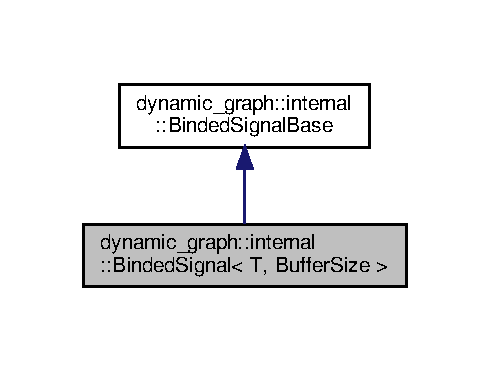
\includegraphics[width=235pt]{structdynamic__graph_1_1internal_1_1BindedSignal__inherit__graph}
\end{center}
\end{figure}


Collaboration diagram for dynamic\+\_\+graph\+:\+:internal\+:\+:Binded\+Signal$<$ T, Buffer\+Size $>$\+:
\nopagebreak
\begin{figure}[H]
\begin{center}
\leavevmode
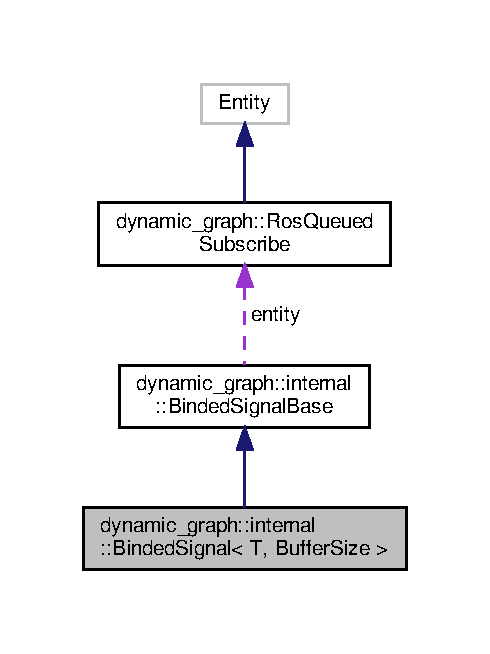
\includegraphics[width=235pt]{structdynamic__graph_1_1internal_1_1BindedSignal__coll__graph}
\end{center}
\end{figure}
\subsection*{Public Types}
\begin{DoxyCompactItemize}
\item 
typedef dynamicgraph\+::\+Signal$<$ T, int $>$ {\bfseries Signal\+\_\+t}\hypertarget{structdynamic__graph_1_1internal_1_1BindedSignal_acdaa84070d25691ad72731f04be389fa}{}\label{structdynamic__graph_1_1internal_1_1BindedSignal_acdaa84070d25691ad72731f04be389fa}

\item 
typedef boost\+::shared\+\_\+ptr$<$ Signal\+\_\+t $>$ {\bfseries Signal\+Ptr\+\_\+t}\hypertarget{structdynamic__graph_1_1internal_1_1BindedSignal_a1fd1a14632e5ebfecd9b32aa3d295194}{}\label{structdynamic__graph_1_1internal_1_1BindedSignal_a1fd1a14632e5ebfecd9b32aa3d295194}

\item 
typedef std\+::vector$<$ T $>$ {\bfseries buffer\+\_\+t}\hypertarget{structdynamic__graph_1_1internal_1_1BindedSignal_a16a9c323d576287f0f053236b43ec78e}{}\label{structdynamic__graph_1_1internal_1_1BindedSignal_a16a9c323d576287f0f053236b43ec78e}

\item 
typedef buffer\+\_\+t\+::size\+\_\+type {\bfseries size\+\_\+type}\hypertarget{structdynamic__graph_1_1internal_1_1BindedSignal_a20afb053e85bdb54b31702d0d58ded53}{}\label{structdynamic__graph_1_1internal_1_1BindedSignal_a20afb053e85bdb54b31702d0d58ded53}

\end{DoxyCompactItemize}
\subsection*{Public Member Functions}
\begin{DoxyCompactItemize}
\item 
{\bfseries Binded\+Signal} (\hyperlink{classdynamic__graph_1_1RosQueuedSubscribe}{Ros\+Queued\+Subscribe} $\ast$e)\hypertarget{structdynamic__graph_1_1internal_1_1BindedSignal_ae6c7caaafe3050957700695604ec9c08}{}\label{structdynamic__graph_1_1internal_1_1BindedSignal_ae6c7caaafe3050957700695604ec9c08}

\item 
void \hyperlink{structdynamic__graph_1_1internal_1_1BindedSignal_a8d377e90b7ece8b1861ddcfa8c7617c8}{clear} ()\hypertarget{structdynamic__graph_1_1internal_1_1BindedSignal_a8d377e90b7ece8b1861ddcfa8c7617c8}{}\label{structdynamic__graph_1_1internal_1_1BindedSignal_a8d377e90b7ece8b1861ddcfa8c7617c8}

\begin{DoxyCompactList}\small\item\em See comments in reader and writer for details about synchronisation. \end{DoxyCompactList}\item 
bool {\bfseries empty} () const \hypertarget{structdynamic__graph_1_1internal_1_1BindedSignal_a6532521e17e7525a4c243c09bd60012a}{}\label{structdynamic__graph_1_1internal_1_1BindedSignal_a6532521e17e7525a4c243c09bd60012a}

\item 
bool {\bfseries full} () const \hypertarget{structdynamic__graph_1_1internal_1_1BindedSignal_aaeafff3cd27d4d3bc566c3d214020e25}{}\label{structdynamic__graph_1_1internal_1_1BindedSignal_aaeafff3cd27d4d3bc566c3d214020e25}

\item 
size\+\_\+type {\bfseries size} () const \hypertarget{structdynamic__graph_1_1internal_1_1BindedSignal_a55f458e8e74049d37c9a034ce334377d}{}\label{structdynamic__graph_1_1internal_1_1BindedSignal_a55f458e8e74049d37c9a034ce334377d}

\item 
{\footnotesize template$<$typename R $>$ }\\void {\bfseries writer} (const R \&data)\hypertarget{structdynamic__graph_1_1internal_1_1BindedSignal_a31010b861170ae56f87a4457b171a1b9}{}\label{structdynamic__graph_1_1internal_1_1BindedSignal_a31010b861170ae56f87a4457b171a1b9}

\item 
T \& {\bfseries reader} (T \&val, int time)\hypertarget{structdynamic__graph_1_1internal_1_1BindedSignal_a292e656913781f59d244df6cfea7ccb0}{}\label{structdynamic__graph_1_1internal_1_1BindedSignal_a292e656913781f59d244df6cfea7ccb0}

\end{DoxyCompactItemize}
\subsection*{Public Attributes}
\begin{DoxyCompactItemize}
\item 
Signal\+Ptr\+\_\+t {\bfseries signal}\hypertarget{structdynamic__graph_1_1internal_1_1BindedSignal_aa0b8c4e3dcea8585de50697b892ea0a4}{}\label{structdynamic__graph_1_1internal_1_1BindedSignal_aa0b8c4e3dcea8585de50697b892ea0a4}

\item 
size\+\_\+type \hyperlink{structdynamic__graph_1_1internal_1_1BindedSignal_af90b4e3d1f26e7525f51e0903c17a37f}{front\+Idx}\hypertarget{structdynamic__graph_1_1internal_1_1BindedSignal_af90b4e3d1f26e7525f51e0903c17a37f}{}\label{structdynamic__graph_1_1internal_1_1BindedSignal_af90b4e3d1f26e7525f51e0903c17a37f}

\begin{DoxyCompactList}\small\item\em Index of the next value to be read. \end{DoxyCompactList}\item 
size\+\_\+type \hyperlink{structdynamic__graph_1_1internal_1_1BindedSignal_a93b1cf4373c6271937f535a68334c523}{back\+Idx}\hypertarget{structdynamic__graph_1_1internal_1_1BindedSignal_a93b1cf4373c6271937f535a68334c523}{}\label{structdynamic__graph_1_1internal_1_1BindedSignal_a93b1cf4373c6271937f535a68334c523}

\begin{DoxyCompactList}\small\item\em Index of the slot where to write next value (does not contain valid data). \end{DoxyCompactList}\item 
buffer\+\_\+t {\bfseries buffer}\hypertarget{structdynamic__graph_1_1internal_1_1BindedSignal_aefa6f66d4def9aa5353335c035c1d716}{}\label{structdynamic__graph_1_1internal_1_1BindedSignal_aefa6f66d4def9aa5353335c035c1d716}

\item 
boost\+::mutex {\bfseries wmutex}\hypertarget{structdynamic__graph_1_1internal_1_1BindedSignal_ad3b9957dafb9684643caacbdc2739c38}{}\label{structdynamic__graph_1_1internal_1_1BindedSignal_ad3b9957dafb9684643caacbdc2739c38}

\item 
boost\+::mutex {\bfseries rmutex}\hypertarget{structdynamic__graph_1_1internal_1_1BindedSignal_a25a7206b3a9904d4cccd226bd885e232}{}\label{structdynamic__graph_1_1internal_1_1BindedSignal_a25a7206b3a9904d4cccd226bd885e232}

\item 
T {\bfseries last}\hypertarget{structdynamic__graph_1_1internal_1_1BindedSignal_a23688c234ce0c8935ed3f52783fa9f2a}{}\label{structdynamic__graph_1_1internal_1_1BindedSignal_a23688c234ce0c8935ed3f52783fa9f2a}

\item 
bool {\bfseries init}\hypertarget{structdynamic__graph_1_1internal_1_1BindedSignal_ac2169fa9a731a30f66805c53af7f55eb}{}\label{structdynamic__graph_1_1internal_1_1BindedSignal_ac2169fa9a731a30f66805c53af7f55eb}

\end{DoxyCompactItemize}


The documentation for this struct was generated from the following files\+:\begin{DoxyCompactItemize}
\item 
include/ros\+\_\+entities/\hyperlink{ros__queued__subscribe_8hh}{ros\+\_\+queued\+\_\+subscribe.\+hh}\item 
include/ros\+\_\+entities/\hyperlink{ros__queued__subscribe_8hxx}{ros\+\_\+queued\+\_\+subscribe.\+hxx}\end{DoxyCompactItemize}

\hypertarget{structdynamic__graph_1_1internal_1_1BindedSignalBase}{}\section{dynamic\+\_\+graph\+:\+:internal\+:\+:Binded\+Signal\+Base Struct Reference}
\label{structdynamic__graph_1_1internal_1_1BindedSignalBase}\index{dynamic\+\_\+graph\+::internal\+::\+Binded\+Signal\+Base@{dynamic\+\_\+graph\+::internal\+::\+Binded\+Signal\+Base}}


Inheritance diagram for dynamic\+\_\+graph\+:\+:internal\+:\+:Binded\+Signal\+Base\+:
\nopagebreak
\begin{figure}[H]
\begin{center}
\leavevmode
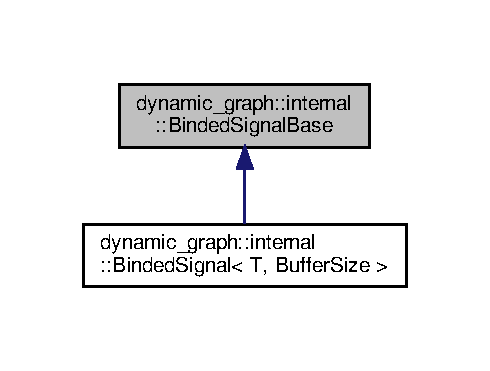
\includegraphics[width=235pt]{structdynamic__graph_1_1internal_1_1BindedSignalBase__inherit__graph}
\end{center}
\end{figure}


Collaboration diagram for dynamic\+\_\+graph\+:\+:internal\+:\+:Binded\+Signal\+Base\+:
\nopagebreak
\begin{figure}[H]
\begin{center}
\leavevmode
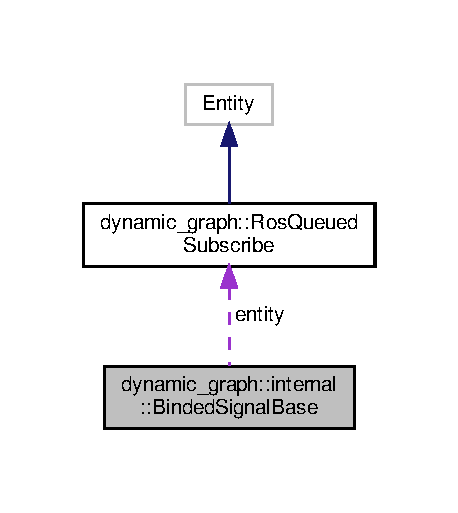
\includegraphics[width=220pt]{structdynamic__graph_1_1internal_1_1BindedSignalBase__coll__graph}
\end{center}
\end{figure}
\subsection*{Public Types}
\begin{DoxyCompactItemize}
\item 
typedef boost\+::shared\+\_\+ptr$<$ ros\+::\+Subscriber $>$ {\bfseries Subscriber\+\_\+t}\hypertarget{structdynamic__graph_1_1internal_1_1BindedSignalBase_a1933d9d9542b368db7cc0bfb9f815aca}{}\label{structdynamic__graph_1_1internal_1_1BindedSignalBase_a1933d9d9542b368db7cc0bfb9f815aca}

\end{DoxyCompactItemize}
\subsection*{Public Member Functions}
\begin{DoxyCompactItemize}
\item 
{\bfseries Binded\+Signal\+Base} (\hyperlink{classdynamic__graph_1_1RosQueuedSubscribe}{Ros\+Queued\+Subscribe} $\ast$e)\hypertarget{structdynamic__graph_1_1internal_1_1BindedSignalBase_a26dec102614700c0ee2e7ad82dade3fe}{}\label{structdynamic__graph_1_1internal_1_1BindedSignalBase_a26dec102614700c0ee2e7ad82dade3fe}

\item 
virtual void {\bfseries clear} ()=0\hypertarget{structdynamic__graph_1_1internal_1_1BindedSignalBase_a65e4a7c402753871fb2b6ca25a4f7b04}{}\label{structdynamic__graph_1_1internal_1_1BindedSignalBase_a65e4a7c402753871fb2b6ca25a4f7b04}

\item 
virtual std\+::size\+\_\+t {\bfseries size} () const =0\hypertarget{structdynamic__graph_1_1internal_1_1BindedSignalBase_acd1d899c6da6c8837f1df5c257d13169}{}\label{structdynamic__graph_1_1internal_1_1BindedSignalBase_acd1d899c6da6c8837f1df5c257d13169}

\end{DoxyCompactItemize}
\subsection*{Public Attributes}
\begin{DoxyCompactItemize}
\item 
Subscriber\+\_\+t {\bfseries subscriber}\hypertarget{structdynamic__graph_1_1internal_1_1BindedSignalBase_ad02d78850a029fc9296536a85c414ccb}{}\label{structdynamic__graph_1_1internal_1_1BindedSignalBase_ad02d78850a029fc9296536a85c414ccb}

\item 
\hyperlink{classdynamic__graph_1_1RosQueuedSubscribe}{Ros\+Queued\+Subscribe} $\ast$ {\bfseries entity}\hypertarget{structdynamic__graph_1_1internal_1_1BindedSignalBase_ad755497fd34b1e59650bc290150ff931}{}\label{structdynamic__graph_1_1internal_1_1BindedSignalBase_ad755497fd34b1e59650bc290150ff931}

\end{DoxyCompactItemize}


The documentation for this struct was generated from the following file\+:\begin{DoxyCompactItemize}
\item 
include/ros\+\_\+entities/\hyperlink{ros__queued__subscribe_8hh}{ros\+\_\+queued\+\_\+subscribe.\+hh}\end{DoxyCompactItemize}

\hypertarget{classdynamic__graph_1_1Device}{}\section{dynamic\+\_\+graph\+:\+:Device Class Reference}
\label{classdynamic__graph_1_1Device}\index{dynamic\+\_\+graph\+::\+Device@{dynamic\+\_\+graph\+::\+Device}}


Inheritance diagram for dynamic\+\_\+graph\+:\+:Device\+:
\nopagebreak
\begin{figure}[H]
\begin{center}
\leavevmode
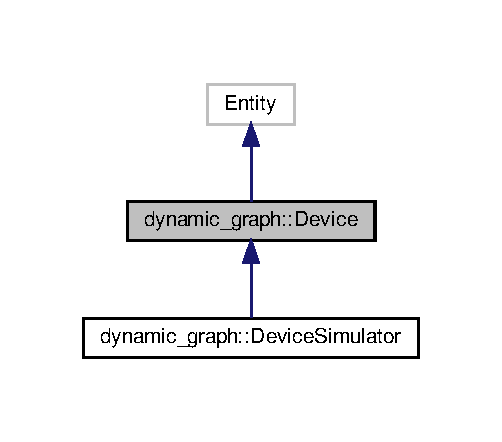
\includegraphics[width=241pt]{classdynamic__graph_1_1Device__inherit__graph}
\end{center}
\end{figure}


Collaboration diagram for dynamic\+\_\+graph\+:\+:Device\+:
\nopagebreak
\begin{figure}[H]
\begin{center}
\leavevmode
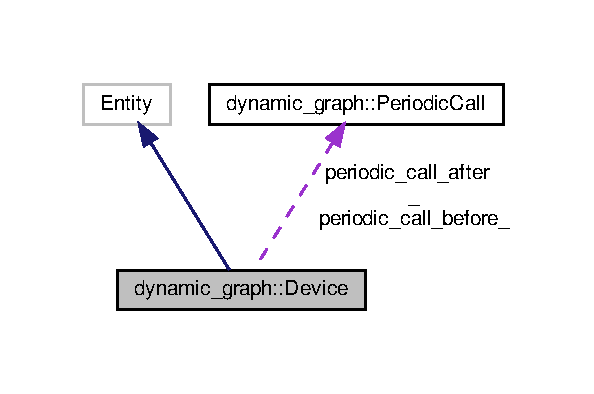
\includegraphics[width=286pt]{classdynamic__graph_1_1Device__coll__graph}
\end{center}
\end{figure}
\subsection*{Public Member Functions}
\begin{DoxyCompactItemize}
\item 
virtual const std\+::string \& \hyperlink{classdynamic__graph_1_1Device_a2aa0523e36b0818e98ad8b12ce7ade6d}{get\+Class\+Name} (void) const 
\begin{DoxyCompactList}\small\item\em get\+Class\+Name is an overloaded function from the class Entity. \end{DoxyCompactList}\item 
\hyperlink{classdynamic__graph_1_1Device_a76c80f6d47e2151494e375e2faf78c0d}{Device} (const std\+::string \&input\+\_\+name)
\begin{DoxyCompactList}\small\item\em \hyperlink{classdynamic__graph_1_1Device}{Device} is the constructor. \end{DoxyCompactList}\item 
virtual \hyperlink{classdynamic__graph_1_1Device_a9dabc419c8d8df3a686c33ce042bc99a}{$\sim$\+Device} ()\hypertarget{classdynamic__graph_1_1Device_a9dabc419c8d8df3a686c33ce042bc99a}{}\label{classdynamic__graph_1_1Device_a9dabc419c8d8df3a686c33ce042bc99a}

\begin{DoxyCompactList}\small\item\em $\sim$\+Device is a default destructor that might overloaded \end{DoxyCompactList}\item 
virtual void \hyperlink{classdynamic__graph_1_1Device_af6edd01afac2838c4e336c76caa4338a}{initialize} (const Y\+A\+M\+L\+::\+Node \&params)
\begin{DoxyCompactList}\small\item\em initialize is the function that initialize the device from the Y\+A\+ML paramters \end{DoxyCompactList}\item 
virtual void \hyperlink{classdynamic__graph_1_1Device_af71d151e69555e9530d770d3d90b7f3e}{initialize\+\_\+from\+\_\+file} (const std\+::string \&yaml\+\_\+file)
\begin{DoxyCompactList}\small\item\em initialize\+\_\+from\+\_\+file is the function that initialize the device from a Y\+A\+ML file. \end{DoxyCompactList}\item 
void \hyperlink{classdynamic__graph_1_1Device_ac4203f6753b2d534c0ade84fb52ac47e}{initialize\+\_\+maps} (const Y\+A\+M\+L\+::\+Node \&sensors\+\_\+and\+\_\+controls)\hypertarget{classdynamic__graph_1_1Device_ac4203f6753b2d534c0ade84fb52ac47e}{}\label{classdynamic__graph_1_1Device_ac4203f6753b2d534c0ade84fb52ac47e}

\begin{DoxyCompactList}\small\item\em parse\+\_\+yaml\+\_\+file fill in the internal maps for sensors and controls. \end{DoxyCompactList}\item 
virtual void \hyperlink{classdynamic__graph_1_1Device_ab8dc9a016ebbc34521812a27b5aa6efa}{set\+\_\+sensors\+\_\+from\+\_\+map} (const \hyperlink{namespacedynamic__graph_a51212ed7fa4ae81e7b362a27f09b7ab8}{Vector\+D\+G\+Map} \&sensors)
\begin{DoxyCompactList}\small\item\em set\+\_\+sensors\+\_\+from\+\_\+map is a parser that feed the map \char`\"{}sensors\char`\"{} with the hardware sensor readings. \end{DoxyCompactList}\item 
virtual void \hyperlink{classdynamic__graph_1_1Device_adb596e7acd67089bb4929cf577b3c6ff}{execute\+\_\+graph} ()
\begin{DoxyCompactList}\small\item\em execute\+\_\+graph is a fonction that execute the graph. \end{DoxyCompactList}\item 
void \hyperlink{classdynamic__graph_1_1Device_a126268314fea8fff802fc957cbf3e0d7}{execute\+\_\+graph\+\_\+deprecated} ()
\begin{DoxyCompactList}\small\item\em execute\+\_\+graph is a fonction that execute the graph. \end{DoxyCompactList}\item 
virtual void \hyperlink{classdynamic__graph_1_1Device_a3291a91974c35f03719220e237512aa8}{get\+\_\+controls\+\_\+to\+\_\+map} (\hyperlink{namespacedynamic__graph_a51212ed7fa4ae81e7b362a27f09b7ab8}{Vector\+D\+G\+Map} \&motor\+\_\+controls)
\begin{DoxyCompactList}\small\item\em get\+\_\+controls\+\_\+to\+\_\+map is a parser that feed the map \char`\"{}controls\char`\"{} with the output of the Dynamic\+Graph. \end{DoxyCompactList}\end{DoxyCompactItemize}
\subsection*{Public Attributes}
\begin{DoxyCompactItemize}
\item 
Device\+Out\+Signal\+Map \hyperlink{classdynamic__graph_1_1Device_ab397e65116cdc32ffa767bfc92c0b7e0}{sensors\+\_\+out\+\_\+}
\begin{DoxyCompactList}\small\item\em sensors\+\_\+out\+\_\+ is a map of device output signals. \end{DoxyCompactList}\item 
\hyperlink{namespacedynamic__graph_a51212ed7fa4ae81e7b362a27f09b7ab8}{Vector\+D\+G\+Map} \hyperlink{classdynamic__graph_1_1Device_a338b04580b75994516b8cc04d6605541}{sensors\+\_\+map\+\_\+}
\begin{DoxyCompactList}\small\item\em sensors\+\_\+map\+\_\+ is a map of dynamicgraph\+::\+Vector. \end{DoxyCompactList}\item 
Device\+In\+Signal\+Map \hyperlink{classdynamic__graph_1_1Device_a77f0617d7b53fb47d77af7557521daf4}{motor\+\_\+controls\+\_\+in\+\_\+}
\begin{DoxyCompactList}\small\item\em motor\+\_\+control\+\_\+in\+\_\+ is the output motor control for each joint. \end{DoxyCompactList}\item 
\hyperlink{namespacedynamic__graph_a51212ed7fa4ae81e7b362a27f09b7ab8}{Vector\+D\+G\+Map} \hyperlink{classdynamic__graph_1_1Device_a9d866a7e294a7445fb88dee8d8a80851}{motor\+\_\+controls\+\_\+map\+\_\+}
\begin{DoxyCompactList}\small\item\em motor\+\_\+controls\+\_\+map\+\_\+ is a map of dynamicgraph\+::\+Vector. \end{DoxyCompactList}\end{DoxyCompactItemize}
\subsection*{Static Public Attributes}
\begin{DoxyCompactItemize}
\item 
static const std\+::string \hyperlink{classdynamic__graph_1_1Device_ab1612928a8cf1a9133fb2571f99095b1}{C\+L\+A\+S\+S\+\_\+\+N\+A\+ME}\hypertarget{classdynamic__graph_1_1Device_ab1612928a8cf1a9133fb2571f99095b1}{}\label{classdynamic__graph_1_1Device_ab1612928a8cf1a9133fb2571f99095b1}

\begin{DoxyCompactList}\small\item\em This is the name of the classe that is used to store the object in the dynamic graph. \end{DoxyCompactList}\end{DoxyCompactItemize}
\subsection*{Protected Attributes}
\begin{DoxyCompactItemize}
\item 
\hyperlink{classdynamic__graph_1_1PeriodicCall}{Periodic\+Call} \hyperlink{classdynamic__graph_1_1Device_afe6456e2d14701498bde6ed74fb0526a}{periodic\+\_\+call\+\_\+before\+\_\+}
\begin{DoxyCompactList}\small\item\em periodic\+\_\+call\+\_\+before\+\_\+ handle the {\itshape synchronous} command call on the device between getting the sensor data and sending the commands. \end{DoxyCompactList}\item 
\hyperlink{classdynamic__graph_1_1PeriodicCall}{Periodic\+Call} \hyperlink{classdynamic__graph_1_1Device_aa2ff18a40858856c9be43b2d609d63ab}{periodic\+\_\+call\+\_\+after\+\_\+}
\begin{DoxyCompactList}\small\item\em periodic\+\_\+call\+\_\+after\+\_\+ handle the {\itshape synchronous} command call on the device between getting the sensor data and sending the commands. \end{DoxyCompactList}\item 
Y\+A\+M\+L\+::\+Node \hyperlink{classdynamic__graph_1_1Device_a9dc0a118c20e33194463eff1c18ce247}{params\+\_\+}\hypertarget{classdynamic__graph_1_1Device_a9dc0a118c20e33194463eff1c18ce247}{}\label{classdynamic__graph_1_1Device_a9dc0a118c20e33194463eff1c18ce247}

\begin{DoxyCompactList}\small\item\em params is a Y\+A\+ML node that allow the creation of a modular device \end{DoxyCompactList}\end{DoxyCompactItemize}


\subsection{Constructor \& Destructor Documentation}
\index{dynamic\+\_\+graph\+::\+Device@{dynamic\+\_\+graph\+::\+Device}!Device@{Device}}
\index{Device@{Device}!dynamic\+\_\+graph\+::\+Device@{dynamic\+\_\+graph\+::\+Device}}
\subsubsection[{\texorpdfstring{Device(const std\+::string \&input\+\_\+name)}{Device(const std::string &input_name)}}]{\setlength{\rightskip}{0pt plus 5cm}Device\+::\+Device (
\begin{DoxyParamCaption}
\item[{const std\+::string \&}]{input\+\_\+name}
\end{DoxyParamCaption}
)}\hypertarget{classdynamic__graph_1_1Device_a76c80f6d47e2151494e375e2faf78c0d}{}\label{classdynamic__graph_1_1Device_a76c80f6d47e2151494e375e2faf78c0d}


\hyperlink{classdynamic__graph_1_1Device}{Device} is the constructor. 

The name allow the Dynamic\+Graph to identify the entity 
\begin{DoxyParams}{Parameters}
{\em params} & is the yaml file used to initialize the device \\
\hline
\end{DoxyParams}


\subsection{Member Function Documentation}
\index{dynamic\+\_\+graph\+::\+Device@{dynamic\+\_\+graph\+::\+Device}!execute\+\_\+graph@{execute\+\_\+graph}}
\index{execute\+\_\+graph@{execute\+\_\+graph}!dynamic\+\_\+graph\+::\+Device@{dynamic\+\_\+graph\+::\+Device}}
\subsubsection[{\texorpdfstring{execute\+\_\+graph()}{execute_graph()}}]{\setlength{\rightskip}{0pt plus 5cm}void Device\+::execute\+\_\+graph (
\begin{DoxyParamCaption}
{}
\end{DoxyParamCaption}
)\hspace{0.3cm}{\ttfamily [virtual]}}\hypertarget{classdynamic__graph_1_1Device_adb596e7acd67089bb4929cf577b3c6ff}{}\label{classdynamic__graph_1_1Device_adb596e7acd67089bb4929cf577b3c6ff}


execute\+\_\+graph is a fonction that execute the graph. 

In order it does\+:
\begin{DoxyItemize}
\item Execute a first set of synchrounous commands.
\item Execute the graph.
\item Execute a second set of synchronous commands. 
\end{DoxyItemize}

Reimplemented in \hyperlink{classdynamic__graph_1_1DeviceSimulator_a614c51ee8d55765019ae98715f875ed5}{dynamic\+\_\+graph\+::\+Device\+Simulator}.

\index{dynamic\+\_\+graph\+::\+Device@{dynamic\+\_\+graph\+::\+Device}!execute\+\_\+graph\+\_\+deprecated@{execute\+\_\+graph\+\_\+deprecated}}
\index{execute\+\_\+graph\+\_\+deprecated@{execute\+\_\+graph\+\_\+deprecated}!dynamic\+\_\+graph\+::\+Device@{dynamic\+\_\+graph\+::\+Device}}
\subsubsection[{\texorpdfstring{execute\+\_\+graph\+\_\+deprecated()}{execute_graph_deprecated()}}]{\setlength{\rightskip}{0pt plus 5cm}void dynamic\+\_\+graph\+::\+Device\+::execute\+\_\+graph\+\_\+deprecated (
\begin{DoxyParamCaption}
{}
\end{DoxyParamCaption}
)\hspace{0.3cm}{\ttfamily [inline]}}\hypertarget{classdynamic__graph_1_1Device_a126268314fea8fff802fc957cbf3e0d7}{}\label{classdynamic__graph_1_1Device_a126268314fea8fff802fc957cbf3e0d7}


execute\+\_\+graph is a fonction that execute the graph. 

In order it does\+:
\begin{DoxyItemize}
\item Execute a first set of synchrounous commands.
\item Execute the graph.
\item Execute a second set of synchronous commands. 
\end{DoxyItemize}\index{dynamic\+\_\+graph\+::\+Device@{dynamic\+\_\+graph\+::\+Device}!get\+\_\+controls\+\_\+to\+\_\+map@{get\+\_\+controls\+\_\+to\+\_\+map}}
\index{get\+\_\+controls\+\_\+to\+\_\+map@{get\+\_\+controls\+\_\+to\+\_\+map}!dynamic\+\_\+graph\+::\+Device@{dynamic\+\_\+graph\+::\+Device}}
\subsubsection[{\texorpdfstring{get\+\_\+controls\+\_\+to\+\_\+map(\+Vector\+D\+G\+Map \&motor\+\_\+controls)}{get_controls_to_map(VectorDGMap &motor_controls)}}]{\setlength{\rightskip}{0pt plus 5cm}void Device\+::get\+\_\+controls\+\_\+to\+\_\+map (
\begin{DoxyParamCaption}
\item[{{\bf Vector\+D\+G\+Map} \&}]{motor\+\_\+controls}
\end{DoxyParamCaption}
)\hspace{0.3cm}{\ttfamily [virtual]}}\hypertarget{classdynamic__graph_1_1Device_a3291a91974c35f03719220e237512aa8}{}\label{classdynamic__graph_1_1Device_a3291a91974c35f03719220e237512aa8}


get\+\_\+controls\+\_\+to\+\_\+map is a parser that feed the map \char`\"{}controls\char`\"{} with the output of the Dynamic\+Graph. 


\begin{DoxyParams}{Parameters}
{\em controls} & is the map containing the controls. \\
\hline
\end{DoxyParams}
\index{dynamic\+\_\+graph\+::\+Device@{dynamic\+\_\+graph\+::\+Device}!get\+Class\+Name@{get\+Class\+Name}}
\index{get\+Class\+Name@{get\+Class\+Name}!dynamic\+\_\+graph\+::\+Device@{dynamic\+\_\+graph\+::\+Device}}
\subsubsection[{\texorpdfstring{get\+Class\+Name(void) const }{getClassName(void) const }}]{\setlength{\rightskip}{0pt plus 5cm}virtual const std\+::string\& dynamic\+\_\+graph\+::\+Device\+::get\+Class\+Name (
\begin{DoxyParamCaption}
\item[{void}]{}
\end{DoxyParamCaption}
) const\hspace{0.3cm}{\ttfamily [inline]}, {\ttfamily [virtual]}}\hypertarget{classdynamic__graph_1_1Device_a2aa0523e36b0818e98ad8b12ce7ade6d}{}\label{classdynamic__graph_1_1Device_a2aa0523e36b0818e98ad8b12ce7ade6d}


get\+Class\+Name is an overloaded function from the class Entity. 

It is used to access the class name and do \begin{DoxyReturn}{Returns}
the name of the device class 
\end{DoxyReturn}
\index{dynamic\+\_\+graph\+::\+Device@{dynamic\+\_\+graph\+::\+Device}!initialize@{initialize}}
\index{initialize@{initialize}!dynamic\+\_\+graph\+::\+Device@{dynamic\+\_\+graph\+::\+Device}}
\subsubsection[{\texorpdfstring{initialize(const Y\+A\+M\+L\+::\+Node \&params)}{initialize(const YAML::Node &params)}}]{\setlength{\rightskip}{0pt plus 5cm}void Device\+::initialize (
\begin{DoxyParamCaption}
\item[{const Y\+A\+M\+L\+::\+Node \&}]{params}
\end{DoxyParamCaption}
)\hspace{0.3cm}{\ttfamily [virtual]}}\hypertarget{classdynamic__graph_1_1Device_af6edd01afac2838c4e336c76caa4338a}{}\label{classdynamic__graph_1_1Device_af6edd01afac2838c4e336c76caa4338a}


initialize is the function that initialize the device from the Y\+A\+ML paramters 


\begin{DoxyParams}{Parameters}
{\em params} & is the yaml file used to initialize the device \\
\hline
\end{DoxyParams}


Reimplemented in \hyperlink{classdynamic__graph_1_1DeviceSimulator_a346995902653feca7707f8c62ab4bf95}{dynamic\+\_\+graph\+::\+Device\+Simulator}.

\index{dynamic\+\_\+graph\+::\+Device@{dynamic\+\_\+graph\+::\+Device}!initialize\+\_\+from\+\_\+file@{initialize\+\_\+from\+\_\+file}}
\index{initialize\+\_\+from\+\_\+file@{initialize\+\_\+from\+\_\+file}!dynamic\+\_\+graph\+::\+Device@{dynamic\+\_\+graph\+::\+Device}}
\subsubsection[{\texorpdfstring{initialize\+\_\+from\+\_\+file(const std\+::string \&yaml\+\_\+file)}{initialize_from_file(const std::string &yaml_file)}}]{\setlength{\rightskip}{0pt plus 5cm}void Device\+::initialize\+\_\+from\+\_\+file (
\begin{DoxyParamCaption}
\item[{const std\+::string \&}]{yaml\+\_\+file}
\end{DoxyParamCaption}
)\hspace{0.3cm}{\ttfamily [virtual]}}\hypertarget{classdynamic__graph_1_1Device_af71d151e69555e9530d770d3d90b7f3e}{}\label{classdynamic__graph_1_1Device_af71d151e69555e9530d770d3d90b7f3e}


initialize\+\_\+from\+\_\+file is the function that initialize the device from a Y\+A\+ML file. 

It loads internally the file and then use the paramters to initialize itself using the \char`\"{}initialize\char`\"{} method. 
\begin{DoxyParams}{Parameters}
{\em params} & is the yaml file used to initialize the device \\
\hline
\end{DoxyParams}


Reimplemented in \hyperlink{classdynamic__graph_1_1DeviceSimulator_a8a9370f236ba03162be2472c79f865f2}{dynamic\+\_\+graph\+::\+Device\+Simulator}.

\index{dynamic\+\_\+graph\+::\+Device@{dynamic\+\_\+graph\+::\+Device}!set\+\_\+sensors\+\_\+from\+\_\+map@{set\+\_\+sensors\+\_\+from\+\_\+map}}
\index{set\+\_\+sensors\+\_\+from\+\_\+map@{set\+\_\+sensors\+\_\+from\+\_\+map}!dynamic\+\_\+graph\+::\+Device@{dynamic\+\_\+graph\+::\+Device}}
\subsubsection[{\texorpdfstring{set\+\_\+sensors\+\_\+from\+\_\+map(const Vector\+D\+G\+Map \&sensors)}{set_sensors_from_map(const VectorDGMap &sensors)}}]{\setlength{\rightskip}{0pt plus 5cm}void Device\+::set\+\_\+sensors\+\_\+from\+\_\+map (
\begin{DoxyParamCaption}
\item[{const {\bf Vector\+D\+G\+Map} \&}]{sensors}
\end{DoxyParamCaption}
)\hspace{0.3cm}{\ttfamily [virtual]}}\hypertarget{classdynamic__graph_1_1Device_ab8dc9a016ebbc34521812a27b5aa6efa}{}\label{classdynamic__graph_1_1Device_ab8dc9a016ebbc34521812a27b5aa6efa}


set\+\_\+sensors\+\_\+from\+\_\+map is a parser that feed the map \char`\"{}sensors\char`\"{} with the hardware sensor readings. 


\begin{DoxyParams}{Parameters}
{\em sensors} & the sensors data. \\
\hline
\end{DoxyParams}


\subsection{Member Data Documentation}
\index{dynamic\+\_\+graph\+::\+Device@{dynamic\+\_\+graph\+::\+Device}!motor\+\_\+controls\+\_\+in\+\_\+@{motor\+\_\+controls\+\_\+in\+\_\+}}
\index{motor\+\_\+controls\+\_\+in\+\_\+@{motor\+\_\+controls\+\_\+in\+\_\+}!dynamic\+\_\+graph\+::\+Device@{dynamic\+\_\+graph\+::\+Device}}
\subsubsection[{\texorpdfstring{motor\+\_\+controls\+\_\+in\+\_\+}{motor_controls_in_}}]{\setlength{\rightskip}{0pt plus 5cm}Device\+In\+Signal\+Map dynamic\+\_\+graph\+::\+Device\+::motor\+\_\+controls\+\_\+in\+\_\+}\hypertarget{classdynamic__graph_1_1Device_a77f0617d7b53fb47d77af7557521daf4}{}\label{classdynamic__graph_1_1Device_a77f0617d7b53fb47d77af7557521daf4}


motor\+\_\+control\+\_\+in\+\_\+ is the output motor control for each joint. 

Feeding this signal {\itshape IS M\+A\+N\+D\+A\+T\+O\+RY} otherwise accessing this data will make the process crash. \index{dynamic\+\_\+graph\+::\+Device@{dynamic\+\_\+graph\+::\+Device}!motor\+\_\+controls\+\_\+map\+\_\+@{motor\+\_\+controls\+\_\+map\+\_\+}}
\index{motor\+\_\+controls\+\_\+map\+\_\+@{motor\+\_\+controls\+\_\+map\+\_\+}!dynamic\+\_\+graph\+::\+Device@{dynamic\+\_\+graph\+::\+Device}}
\subsubsection[{\texorpdfstring{motor\+\_\+controls\+\_\+map\+\_\+}{motor_controls_map_}}]{\setlength{\rightskip}{0pt plus 5cm}{\bf Vector\+D\+G\+Map} dynamic\+\_\+graph\+::\+Device\+::motor\+\_\+controls\+\_\+map\+\_\+}\hypertarget{classdynamic__graph_1_1Device_a9d866a7e294a7445fb88dee8d8a80851}{}\label{classdynamic__graph_1_1Device_a9d866a7e294a7445fb88dee8d8a80851}


motor\+\_\+controls\+\_\+map\+\_\+ is a map of dynamicgraph\+::\+Vector. 

They represent all the controls to be sent to the robot. \index{dynamic\+\_\+graph\+::\+Device@{dynamic\+\_\+graph\+::\+Device}!periodic\+\_\+call\+\_\+after\+\_\+@{periodic\+\_\+call\+\_\+after\+\_\+}}
\index{periodic\+\_\+call\+\_\+after\+\_\+@{periodic\+\_\+call\+\_\+after\+\_\+}!dynamic\+\_\+graph\+::\+Device@{dynamic\+\_\+graph\+::\+Device}}
\subsubsection[{\texorpdfstring{periodic\+\_\+call\+\_\+after\+\_\+}{periodic_call_after_}}]{\setlength{\rightskip}{0pt plus 5cm}{\bf Periodic\+Call} dynamic\+\_\+graph\+::\+Device\+::periodic\+\_\+call\+\_\+after\+\_\+\hspace{0.3cm}{\ttfamily [protected]}}\hypertarget{classdynamic__graph_1_1Device_aa2ff18a40858856c9be43b2d609d63ab}{}\label{classdynamic__graph_1_1Device_aa2ff18a40858856c9be43b2d609d63ab}


periodic\+\_\+call\+\_\+after\+\_\+ handle the {\itshape synchronous} command call on the device between getting the sensor data and sending the commands. 

Typically used when one wants to evaluate a signal that is not plugged. \index{dynamic\+\_\+graph\+::\+Device@{dynamic\+\_\+graph\+::\+Device}!periodic\+\_\+call\+\_\+before\+\_\+@{periodic\+\_\+call\+\_\+before\+\_\+}}
\index{periodic\+\_\+call\+\_\+before\+\_\+@{periodic\+\_\+call\+\_\+before\+\_\+}!dynamic\+\_\+graph\+::\+Device@{dynamic\+\_\+graph\+::\+Device}}
\subsubsection[{\texorpdfstring{periodic\+\_\+call\+\_\+before\+\_\+}{periodic_call_before_}}]{\setlength{\rightskip}{0pt plus 5cm}{\bf Periodic\+Call} dynamic\+\_\+graph\+::\+Device\+::periodic\+\_\+call\+\_\+before\+\_\+\hspace{0.3cm}{\ttfamily [protected]}}\hypertarget{classdynamic__graph_1_1Device_afe6456e2d14701498bde6ed74fb0526a}{}\label{classdynamic__graph_1_1Device_afe6456e2d14701498bde6ed74fb0526a}


periodic\+\_\+call\+\_\+before\+\_\+ handle the {\itshape synchronous} command call on the device between getting the sensor data and sending the commands. 

Typically used when one wants to evaluate a signal that is not plugged. \index{dynamic\+\_\+graph\+::\+Device@{dynamic\+\_\+graph\+::\+Device}!sensors\+\_\+map\+\_\+@{sensors\+\_\+map\+\_\+}}
\index{sensors\+\_\+map\+\_\+@{sensors\+\_\+map\+\_\+}!dynamic\+\_\+graph\+::\+Device@{dynamic\+\_\+graph\+::\+Device}}
\subsubsection[{\texorpdfstring{sensors\+\_\+map\+\_\+}{sensors_map_}}]{\setlength{\rightskip}{0pt plus 5cm}{\bf Vector\+D\+G\+Map} dynamic\+\_\+graph\+::\+Device\+::sensors\+\_\+map\+\_\+}\hypertarget{classdynamic__graph_1_1Device_a338b04580b75994516b8cc04d6605541}{}\label{classdynamic__graph_1_1Device_a338b04580b75994516b8cc04d6605541}


sensors\+\_\+map\+\_\+ is a map of dynamicgraph\+::\+Vector. 

They represent all the sensors data measured on the robot. \index{dynamic\+\_\+graph\+::\+Device@{dynamic\+\_\+graph\+::\+Device}!sensors\+\_\+out\+\_\+@{sensors\+\_\+out\+\_\+}}
\index{sensors\+\_\+out\+\_\+@{sensors\+\_\+out\+\_\+}!dynamic\+\_\+graph\+::\+Device@{dynamic\+\_\+graph\+::\+Device}}
\subsubsection[{\texorpdfstring{sensors\+\_\+out\+\_\+}{sensors_out_}}]{\setlength{\rightskip}{0pt plus 5cm}Device\+Out\+Signal\+Map dynamic\+\_\+graph\+::\+Device\+::sensors\+\_\+out\+\_\+}\hypertarget{classdynamic__graph_1_1Device_ab397e65116cdc32ffa767bfc92c0b7e0}{}\label{classdynamic__graph_1_1Device_ab397e65116cdc32ffa767bfc92c0b7e0}


sensors\+\_\+out\+\_\+ is a map of device output signals. 

They represent all the sensors belonging to the robot. 

The documentation for this class was generated from the following files\+:\begin{DoxyCompactItemize}
\item 
include/dynamic\+\_\+graph\+\_\+manager/\hyperlink{device_8hh}{device.\+hh}\item 
src/\hyperlink{device_8cpp}{device.\+cpp}\end{DoxyCompactItemize}

\hypertarget{classdynamic__graph_1_1DeviceSimulator}{}\section{dynamic\+\_\+graph\+:\+:Device\+Simulator Class Reference}
\label{classdynamic__graph_1_1DeviceSimulator}\index{dynamic\+\_\+graph\+::\+Device\+Simulator@{dynamic\+\_\+graph\+::\+Device\+Simulator}}


Inheritance diagram for dynamic\+\_\+graph\+:\+:Device\+Simulator\+:
\nopagebreak
\begin{figure}[H]
\begin{center}
\leavevmode
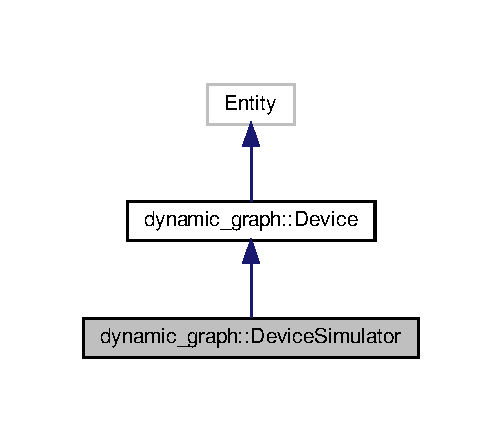
\includegraphics[width=241pt]{classdynamic__graph_1_1DeviceSimulator__inherit__graph}
\end{center}
\end{figure}


Collaboration diagram for dynamic\+\_\+graph\+:\+:Device\+Simulator\+:
\nopagebreak
\begin{figure}[H]
\begin{center}
\leavevmode
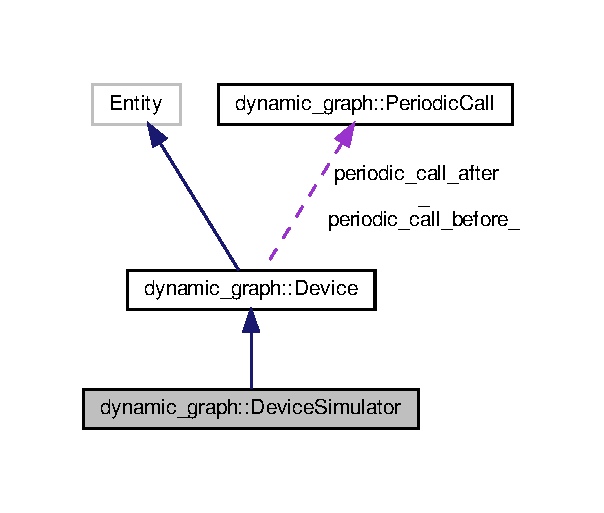
\includegraphics[width=291pt]{classdynamic__graph_1_1DeviceSimulator__coll__graph}
\end{center}
\end{figure}
\subsection*{Public Member Functions}
\begin{DoxyCompactItemize}
\item 
\hyperlink{classdynamic__graph_1_1DeviceSimulator_ad1c52d0a4bfa4617c7653532570a2c90}{Device\+Simulator} (const std\+::string \&input\+\_\+name)
\begin{DoxyCompactList}\small\item\em \hyperlink{classdynamic__graph_1_1DeviceSimulator}{Device\+Simulator} is the constructor. \end{DoxyCompactList}\item 
\hyperlink{classdynamic__graph_1_1DeviceSimulator_a7510771e215f2f20f05a5d4193dc4f76}{$\sim$\+Device\+Simulator} ()\hypertarget{classdynamic__graph_1_1DeviceSimulator_a7510771e215f2f20f05a5d4193dc4f76}{}\label{classdynamic__graph_1_1DeviceSimulator_a7510771e215f2f20f05a5d4193dc4f76}

\begin{DoxyCompactList}\small\item\em Destroy the \hyperlink{classdynamic__graph_1_1DeviceSimulator}{Device\+Simulator} object. \end{DoxyCompactList}\item 
virtual void \hyperlink{classdynamic__graph_1_1DeviceSimulator_a346995902653feca7707f8c62ab4bf95}{initialize} (const Y\+A\+M\+L\+::\+Node \&params)
\begin{DoxyCompactList}\small\item\em This method is hinerited from the \hyperlink{classdynamic__graph_1_1Device}{Device} class. \end{DoxyCompactList}\item 
virtual void \hyperlink{classdynamic__graph_1_1DeviceSimulator_a8a9370f236ba03162be2472c79f865f2}{initialize\+\_\+from\+\_\+file} (const std\+::string \&yaml\+\_\+file)
\begin{DoxyCompactList}\small\item\em This method is hinerited from the \hyperlink{classdynamic__graph_1_1Device}{Device} class. \end{DoxyCompactList}\item 
virtual void \hyperlink{classdynamic__graph_1_1DeviceSimulator_a614c51ee8d55765019ae98715f875ed5}{execute\+\_\+graph} ()
\begin{DoxyCompactList}\small\item\em This method is hinerited from the \hyperlink{classdynamic__graph_1_1Device}{Device} class. \end{DoxyCompactList}\end{DoxyCompactItemize}
\subsection*{Public Attributes}
\begin{DoxyCompactItemize}
\item 
Device\+Out\+Signal\+Map \hyperlink{classdynamic__graph_1_1DeviceSimulator_abbbcc26f173788b15a395ff87f3925e1}{simu\+\_\+motor\+\_\+controls\+\_\+out\+\_\+}
\begin{DoxyCompactList}\small\item\em simu\+\_\+motor\+\_\+controls\+\_\+out\+\_\+ is the output motor control for each joint. \end{DoxyCompactList}\item 
Device\+In\+Signal\+Map \hyperlink{classdynamic__graph_1_1DeviceSimulator_a8640ee078f06fc5f31efcb2b35c9ed99}{simu\+\_\+sensors\+\_\+in\+\_\+}
\begin{DoxyCompactList}\small\item\em simu\+\_\+sensors\+\_\+in\+\_\+ is a map of device output signals. \end{DoxyCompactList}\end{DoxyCompactItemize}
\subsection*{Static Public Attributes}
\begin{DoxyCompactItemize}
\item 
static const std\+::string \hyperlink{classdynamic__graph_1_1DeviceSimulator_a4f28a1f4a96bdf5a2adf1e1f15a8ab77}{C\+L\+A\+S\+S\+\_\+\+N\+A\+ME}\hypertarget{classdynamic__graph_1_1DeviceSimulator_a4f28a1f4a96bdf5a2adf1e1f15a8ab77}{}\label{classdynamic__graph_1_1DeviceSimulator_a4f28a1f4a96bdf5a2adf1e1f15a8ab77}

\begin{DoxyCompactList}\small\item\em This is the name of the classe that is used to store the object in the dynamic graph. \end{DoxyCompactList}\end{DoxyCompactItemize}
\subsection*{Additional Inherited Members}


\subsection{Constructor \& Destructor Documentation}
\index{dynamic\+\_\+graph\+::\+Device\+Simulator@{dynamic\+\_\+graph\+::\+Device\+Simulator}!Device\+Simulator@{Device\+Simulator}}
\index{Device\+Simulator@{Device\+Simulator}!dynamic\+\_\+graph\+::\+Device\+Simulator@{dynamic\+\_\+graph\+::\+Device\+Simulator}}
\subsubsection[{\texorpdfstring{Device\+Simulator(const std\+::string \&input\+\_\+name)}{DeviceSimulator(const std::string &input_name)}}]{\setlength{\rightskip}{0pt plus 5cm}dynamic\+\_\+graph\+::\+Device\+Simulator\+::\+Device\+Simulator (
\begin{DoxyParamCaption}
\item[{const std\+::string \&}]{input\+\_\+name}
\end{DoxyParamCaption}
)}\hypertarget{classdynamic__graph_1_1DeviceSimulator_ad1c52d0a4bfa4617c7653532570a2c90}{}\label{classdynamic__graph_1_1DeviceSimulator_ad1c52d0a4bfa4617c7653532570a2c90}


\hyperlink{classdynamic__graph_1_1DeviceSimulator}{Device\+Simulator} is the constructor. 

The name allow the Dynamic\+Graph to identify the entity. 
\begin{DoxyParams}[1]{Parameters}
\mbox{\tt in}  & {\em name} & is the Dynamic\+Graph identifyer. \\
\hline
\end{DoxyParams}


\subsection{Member Function Documentation}
\index{dynamic\+\_\+graph\+::\+Device\+Simulator@{dynamic\+\_\+graph\+::\+Device\+Simulator}!execute\+\_\+graph@{execute\+\_\+graph}}
\index{execute\+\_\+graph@{execute\+\_\+graph}!dynamic\+\_\+graph\+::\+Device\+Simulator@{dynamic\+\_\+graph\+::\+Device\+Simulator}}
\subsubsection[{\texorpdfstring{execute\+\_\+graph()}{execute_graph()}}]{\setlength{\rightskip}{0pt plus 5cm}void dynamic\+\_\+graph\+::\+Device\+Simulator\+::execute\+\_\+graph (
\begin{DoxyParamCaption}
{}
\end{DoxyParamCaption}
)\hspace{0.3cm}{\ttfamily [virtual]}}\hypertarget{classdynamic__graph_1_1DeviceSimulator_a614c51ee8d55765019ae98715f875ed5}{}\label{classdynamic__graph_1_1DeviceSimulator_a614c51ee8d55765019ae98715f875ed5}


This method is hinerited from the \hyperlink{classdynamic__graph_1_1Device}{Device} class. 

\char`\"{}execute\+\_\+graph\char`\"{} is the method that execute the graph.

In order it does\+:
\begin{DoxyItemize}
\item {\bfseries  Copy the simulation input sensor into the output sensor signals}
\item Execute a first set of synchrounous commands.
\item Execute the graph.
\item Execute a second set of synchronous commands.
\item {\bfseries  Copy the control input into the simulation control output signals} 
\end{DoxyItemize}

Reimplemented from \hyperlink{classdynamic__graph_1_1Device_adb596e7acd67089bb4929cf577b3c6ff}{dynamic\+\_\+graph\+::\+Device}.

\index{dynamic\+\_\+graph\+::\+Device\+Simulator@{dynamic\+\_\+graph\+::\+Device\+Simulator}!initialize@{initialize}}
\index{initialize@{initialize}!dynamic\+\_\+graph\+::\+Device\+Simulator@{dynamic\+\_\+graph\+::\+Device\+Simulator}}
\subsubsection[{\texorpdfstring{initialize(const Y\+A\+M\+L\+::\+Node \&params)}{initialize(const YAML::Node &params)}}]{\setlength{\rightskip}{0pt plus 5cm}void dynamic\+\_\+graph\+::\+Device\+Simulator\+::initialize (
\begin{DoxyParamCaption}
\item[{const Y\+A\+M\+L\+::\+Node \&}]{params}
\end{DoxyParamCaption}
)\hspace{0.3cm}{\ttfamily [virtual]}}\hypertarget{classdynamic__graph_1_1DeviceSimulator_a346995902653feca7707f8c62ab4bf95}{}\label{classdynamic__graph_1_1DeviceSimulator_a346995902653feca7707f8c62ab4bf95}


This method is hinerited from the \hyperlink{classdynamic__graph_1_1Device}{Device} class. 

\char`\"{}initialize\char`\"{} is the function that initialize the device from the Y\+A\+ML paramters. 
\begin{DoxyParams}{Parameters}
{\em params} & is the yaml file used to initialize the device \\
\hline
\end{DoxyParams}


Reimplemented from \hyperlink{classdynamic__graph_1_1Device_af6edd01afac2838c4e336c76caa4338a}{dynamic\+\_\+graph\+::\+Device}.

\index{dynamic\+\_\+graph\+::\+Device\+Simulator@{dynamic\+\_\+graph\+::\+Device\+Simulator}!initialize\+\_\+from\+\_\+file@{initialize\+\_\+from\+\_\+file}}
\index{initialize\+\_\+from\+\_\+file@{initialize\+\_\+from\+\_\+file}!dynamic\+\_\+graph\+::\+Device\+Simulator@{dynamic\+\_\+graph\+::\+Device\+Simulator}}
\subsubsection[{\texorpdfstring{initialize\+\_\+from\+\_\+file(const std\+::string \&yaml\+\_\+file)}{initialize_from_file(const std::string &yaml_file)}}]{\setlength{\rightskip}{0pt plus 5cm}void dynamic\+\_\+graph\+::\+Device\+Simulator\+::initialize\+\_\+from\+\_\+file (
\begin{DoxyParamCaption}
\item[{const std\+::string \&}]{yaml\+\_\+file}
\end{DoxyParamCaption}
)\hspace{0.3cm}{\ttfamily [virtual]}}\hypertarget{classdynamic__graph_1_1DeviceSimulator_a8a9370f236ba03162be2472c79f865f2}{}\label{classdynamic__graph_1_1DeviceSimulator_a8a9370f236ba03162be2472c79f865f2}


This method is hinerited from the \hyperlink{classdynamic__graph_1_1Device}{Device} class. 

\char`\"{}initialize\+\_\+from\+\_\+file\char`\"{} is the function that initialize the device from a Y\+A\+ML file. It loads internally the file and then use the paramters to initialize itself using the \char`\"{}initialize\char`\"{} method. 
\begin{DoxyParams}{Parameters}
{\em params} & is the yaml file used to initialize the device \\
\hline
\end{DoxyParams}


Reimplemented from \hyperlink{classdynamic__graph_1_1Device_af71d151e69555e9530d770d3d90b7f3e}{dynamic\+\_\+graph\+::\+Device}.



\subsection{Member Data Documentation}
\index{dynamic\+\_\+graph\+::\+Device\+Simulator@{dynamic\+\_\+graph\+::\+Device\+Simulator}!simu\+\_\+motor\+\_\+controls\+\_\+out\+\_\+@{simu\+\_\+motor\+\_\+controls\+\_\+out\+\_\+}}
\index{simu\+\_\+motor\+\_\+controls\+\_\+out\+\_\+@{simu\+\_\+motor\+\_\+controls\+\_\+out\+\_\+}!dynamic\+\_\+graph\+::\+Device\+Simulator@{dynamic\+\_\+graph\+::\+Device\+Simulator}}
\subsubsection[{\texorpdfstring{simu\+\_\+motor\+\_\+controls\+\_\+out\+\_\+}{simu_motor_controls_out_}}]{\setlength{\rightskip}{0pt plus 5cm}Device\+Out\+Signal\+Map dynamic\+\_\+graph\+::\+Device\+Simulator\+::simu\+\_\+motor\+\_\+controls\+\_\+out\+\_\+}\hypertarget{classdynamic__graph_1_1DeviceSimulator_abbbcc26f173788b15a395ff87f3925e1}{}\label{classdynamic__graph_1_1DeviceSimulator_abbbcc26f173788b15a395ff87f3925e1}


simu\+\_\+motor\+\_\+controls\+\_\+out\+\_\+ is the output motor control for each joint. 

They are the simulated signals to be plugged to a simulator wrapped as an entity. \index{dynamic\+\_\+graph\+::\+Device\+Simulator@{dynamic\+\_\+graph\+::\+Device\+Simulator}!simu\+\_\+sensors\+\_\+in\+\_\+@{simu\+\_\+sensors\+\_\+in\+\_\+}}
\index{simu\+\_\+sensors\+\_\+in\+\_\+@{simu\+\_\+sensors\+\_\+in\+\_\+}!dynamic\+\_\+graph\+::\+Device\+Simulator@{dynamic\+\_\+graph\+::\+Device\+Simulator}}
\subsubsection[{\texorpdfstring{simu\+\_\+sensors\+\_\+in\+\_\+}{simu_sensors_in_}}]{\setlength{\rightskip}{0pt plus 5cm}Device\+In\+Signal\+Map dynamic\+\_\+graph\+::\+Device\+Simulator\+::simu\+\_\+sensors\+\_\+in\+\_\+}\hypertarget{classdynamic__graph_1_1DeviceSimulator_a8640ee078f06fc5f31efcb2b35c9ed99}{}\label{classdynamic__graph_1_1DeviceSimulator_a8640ee078f06fc5f31efcb2b35c9ed99}


simu\+\_\+sensors\+\_\+in\+\_\+ is a map of device output signals. 

They represent all the sensors belonging to the robot. Feeding these signals {\bfseries  IS M\+A\+N\+D\+A\+T\+O\+RY } otherwise accessing this data will make the process crash. 

The documentation for this class was generated from the following files\+:\begin{DoxyCompactItemize}
\item 
include/dynamic\+\_\+graph\+\_\+manager/\hyperlink{device__simulator_8hh}{device\+\_\+simulator.\+hh}\item 
src/\hyperlink{device__simulator_8cpp}{device\+\_\+simulator.\+cpp}\end{DoxyCompactItemize}

\hypertarget{classros_1_1dgcompleter_1_1DGCompleter}{}\section{ros.\+dgcompleter.\+D\+G\+Completer Class Reference}
\label{classros_1_1dgcompleter_1_1DGCompleter}\index{ros.\+dgcompleter.\+D\+G\+Completer@{ros.\+dgcompleter.\+D\+G\+Completer}}
\subsection*{Public Member Functions}
\begin{DoxyCompactItemize}
\item 
def \hyperlink{classros_1_1dgcompleter_1_1DGCompleter_a3a83ed364b26688ebccc5aa4dfca6886}{\+\_\+\+\_\+init\+\_\+\+\_\+} (self, client)
\item 
def \hyperlink{classros_1_1dgcompleter_1_1DGCompleter_a0662ed6ab4e56fb2a828c5577e03b41e}{complete} (self, text, state)
\end{DoxyCompactItemize}
\subsection*{Public Attributes}
\begin{DoxyCompactItemize}
\item 
{\bfseries client}\hypertarget{classros_1_1dgcompleter_1_1DGCompleter_afcab03fb8dcc2ed3b536d76369037cde}{}\label{classros_1_1dgcompleter_1_1DGCompleter_afcab03fb8dcc2ed3b536d76369037cde}

\end{DoxyCompactItemize}


\subsection{Constructor \& Destructor Documentation}
\index{ros\+::dgcompleter\+::\+D\+G\+Completer@{ros\+::dgcompleter\+::\+D\+G\+Completer}!\+\_\+\+\_\+init\+\_\+\+\_\+@{\+\_\+\+\_\+init\+\_\+\+\_\+}}
\index{\+\_\+\+\_\+init\+\_\+\+\_\+@{\+\_\+\+\_\+init\+\_\+\+\_\+}!ros\+::dgcompleter\+::\+D\+G\+Completer@{ros\+::dgcompleter\+::\+D\+G\+Completer}}
\subsubsection[{\texorpdfstring{\+\_\+\+\_\+init\+\_\+\+\_\+(self, client)}{__init__(self, client)}}]{\setlength{\rightskip}{0pt plus 5cm}def ros.\+dgcompleter.\+D\+G\+Completer.\+\_\+\+\_\+init\+\_\+\+\_\+ (
\begin{DoxyParamCaption}
\item[{}]{self, }
\item[{}]{client}
\end{DoxyParamCaption}
)}\hypertarget{classros_1_1dgcompleter_1_1DGCompleter_a3a83ed364b26688ebccc5aa4dfca6886}{}\label{classros_1_1dgcompleter_1_1DGCompleter_a3a83ed364b26688ebccc5aa4dfca6886}
\begin{DoxyVerb}Create a new completer for the command line.

Completer([client]) -> completer instance.

Client is a ROS proxy to dynamic_graph run_python_command service.

Completer instances should be used as the completion mechanism of
readline via the set_completer() call:

readline.set_completer(Completer(client).complete)
\end{DoxyVerb}
 

\subsection{Member Function Documentation}
\index{ros\+::dgcompleter\+::\+D\+G\+Completer@{ros\+::dgcompleter\+::\+D\+G\+Completer}!complete@{complete}}
\index{complete@{complete}!ros\+::dgcompleter\+::\+D\+G\+Completer@{ros\+::dgcompleter\+::\+D\+G\+Completer}}
\subsubsection[{\texorpdfstring{complete(self, text, state)}{complete(self, text, state)}}]{\setlength{\rightskip}{0pt plus 5cm}def ros.\+dgcompleter.\+D\+G\+Completer.\+complete (
\begin{DoxyParamCaption}
\item[{}]{self, }
\item[{}]{text, }
\item[{}]{state}
\end{DoxyParamCaption}
)}\hypertarget{classros_1_1dgcompleter_1_1DGCompleter_a0662ed6ab4e56fb2a828c5577e03b41e}{}\label{classros_1_1dgcompleter_1_1DGCompleter_a0662ed6ab4e56fb2a828c5577e03b41e}
\begin{DoxyVerb}Return the next possible completion for 'text'.readline.parse_and_bind("tab: complete")


This is called successively with state == 0, 1, 2, ... until it
returns None.  The completion should begin with 'text'.\end{DoxyVerb}
 

The documentation for this class was generated from the following file\+:\begin{DoxyCompactItemize}
\item 
/home/mnaveau/devel/workspace/src/catkin/dg\+\_\+control/dynamic\+\_\+graph\+\_\+manager/python/dynamic\+\_\+graph\+\_\+manager/ros/dgcompleter.\+py\end{DoxyCompactItemize}

\hypertarget{classdynamic__graph_1_1DgToRos}{}\section{dynamic\+\_\+graph\+:\+:Dg\+To\+Ros$<$ Sot\+Type $>$ Class Template Reference}
\label{classdynamic__graph_1_1DgToRos}\index{dynamic\+\_\+graph\+::\+Dg\+To\+Ros$<$ Sot\+Type $>$@{dynamic\+\_\+graph\+::\+Dg\+To\+Ros$<$ Sot\+Type $>$}}


\hyperlink{classdynamic__graph_1_1DgToRos}{Dg\+To\+Ros} trait type.  




{\ttfamily \#include $<$dg\+\_\+to\+\_\+ros.\+hh$>$}



\subsection{Detailed Description}
\subsubsection*{template$<$typename Sot\+Type$>$\\*
class dynamic\+\_\+graph\+::\+Dg\+To\+Ros$<$ Sot\+Type $>$}

\hyperlink{classdynamic__graph_1_1DgToRos}{Dg\+To\+Ros} trait type. 

This trait provides types associated to a dynamic-\/graph type\+:
\begin{DoxyItemize}
\item R\+OS corresponding type,
\item signal type / input signal type,
\item R\+OS callback type. 
\end{DoxyItemize}

The documentation for this class was generated from the following file\+:\begin{DoxyCompactItemize}
\item 
include/ros\+\_\+entities/\hyperlink{dg__to__ros_8hh}{dg\+\_\+to\+\_\+ros.\+hh}\end{DoxyCompactItemize}

\hypertarget{structdynamic__graph_1_1DgToRos_3_01double_01_4}{}\section{dynamic\+\_\+graph\+:\+:Dg\+To\+Ros$<$ double $>$ Struct Template Reference}
\label{structdynamic__graph_1_1DgToRos_3_01double_01_4}\index{dynamic\+\_\+graph\+::\+Dg\+To\+Ros$<$ double $>$@{dynamic\+\_\+graph\+::\+Dg\+To\+Ros$<$ double $>$}}
\subsection*{Public Types}
\begin{DoxyCompactItemize}
\item 
\mbox{\Hypertarget{structdynamic__graph_1_1DgToRos_3_01double_01_4_a44594fa972d07af2e4805c2e84c4f45a}\label{structdynamic__graph_1_1DgToRos_3_01double_01_4_a44594fa972d07af2e4805c2e84c4f45a}} 
typedef double {\bfseries dg\+\_\+t}
\item 
\mbox{\Hypertarget{structdynamic__graph_1_1DgToRos_3_01double_01_4_ae49e3e9e33c974188b284809c6b83dcf}\label{structdynamic__graph_1_1DgToRos_3_01double_01_4_ae49e3e9e33c974188b284809c6b83dcf}} 
typedef std\+\_\+msgs\+::\+Float64 {\bfseries ros\+\_\+t}
\item 
\mbox{\Hypertarget{structdynamic__graph_1_1DgToRos_3_01double_01_4_a3c544d24a5d2de5f6e296f1344609cac}\label{structdynamic__graph_1_1DgToRos_3_01double_01_4_a3c544d24a5d2de5f6e296f1344609cac}} 
typedef std\+\_\+msgs\+::\+Float64\+Const\+Ptr {\bfseries ros\+\_\+const\+\_\+ptr\+\_\+t}
\item 
\mbox{\Hypertarget{structdynamic__graph_1_1DgToRos_3_01double_01_4_a0bf0169020ac9d1707a8cba283ef27fc}\label{structdynamic__graph_1_1DgToRos_3_01double_01_4_a0bf0169020ac9d1707a8cba283ef27fc}} 
typedef dynamicgraph\+::\+Signal$<$ dg\+\_\+t, int $>$ {\bfseries signal\+\_\+t}
\item 
\mbox{\Hypertarget{structdynamic__graph_1_1DgToRos_3_01double_01_4_ac01fc0b999ff3dc8c4218918ffc2ea78}\label{structdynamic__graph_1_1DgToRos_3_01double_01_4_ac01fc0b999ff3dc8c4218918ffc2ea78}} 
typedef dynamicgraph\+::\+Signal\+Ptr$<$ dg\+\_\+t, int $>$ {\bfseries signal\+In\+\_\+t}
\item 
\mbox{\Hypertarget{structdynamic__graph_1_1DgToRos_3_01double_01_4_accf1efdaf640f51715879d46aed907aa}\label{structdynamic__graph_1_1DgToRos_3_01double_01_4_accf1efdaf640f51715879d46aed907aa}} 
typedef boost\+::function$<$ dg\+\_\+t \&(dg\+\_\+t \&, int)$>$ {\bfseries callback\+\_\+t}
\end{DoxyCompactItemize}
\subsection*{Static Public Member Functions}
\begin{DoxyCompactItemize}
\item 
\mbox{\Hypertarget{structdynamic__graph_1_1DgToRos_3_01double_01_4_ab21237e1e16bdb81d3c31f3be382b8ad}\label{structdynamic__graph_1_1DgToRos_3_01double_01_4_ab21237e1e16bdb81d3c31f3be382b8ad}} 
{\footnotesize template$<$typename S $>$ }\\static void {\bfseries set\+Default} (S \&s)
\item 
\mbox{\Hypertarget{structdynamic__graph_1_1DgToRos_3_01double_01_4_ad6ad3bc75e6e7d80d44fa9d4c9eee4ea}\label{structdynamic__graph_1_1DgToRos_3_01double_01_4_ad6ad3bc75e6e7d80d44fa9d4c9eee4ea}} 
static void {\bfseries set\+Default} (dg\+\_\+t \&s)
\end{DoxyCompactItemize}
\subsection*{Static Public Attributes}
\begin{DoxyCompactItemize}
\item 
\mbox{\Hypertarget{structdynamic__graph_1_1DgToRos_3_01double_01_4_a686b38d74e19c6de7308e8d1ae86cf8c}\label{structdynamic__graph_1_1DgToRos_3_01double_01_4_a686b38d74e19c6de7308e8d1ae86cf8c}} 
static const char $\ast$ {\bfseries signal\+Type\+Name} = \char`\"{}Double\char`\"{}
\end{DoxyCompactItemize}


The documentation for this struct was generated from the following files\+:\begin{DoxyCompactItemize}
\item 
include/ros\+\_\+entities/\hyperlink{dg__to__ros_8hh}{dg\+\_\+to\+\_\+ros.\+hh}\item 
src/ros\+\_\+entities/\hyperlink{dg__to__ros_8cpp}{dg\+\_\+to\+\_\+ros.\+cpp}\end{DoxyCompactItemize}

\hypertarget{structdynamic__graph_1_1DgToRos_3_01Matrix_01_4}{}\section{dynamic\+\_\+graph\+:\+:Dg\+To\+Ros$<$ Matrix $>$ Struct Template Reference}
\label{structdynamic__graph_1_1DgToRos_3_01Matrix_01_4}\index{dynamic\+\_\+graph\+::\+Dg\+To\+Ros$<$ Matrix $>$@{dynamic\+\_\+graph\+::\+Dg\+To\+Ros$<$ Matrix $>$}}
\subsection*{Public Types}
\begin{DoxyCompactItemize}
\item 
typedef Matrix {\bfseries dg\+\_\+t}\hypertarget{structdynamic__graph_1_1DgToRos_3_01Matrix_01_4_af6e44b5062891d225b02936ff788476a}{}\label{structdynamic__graph_1_1DgToRos_3_01Matrix_01_4_af6e44b5062891d225b02936ff788476a}

\item 
typedef dynamic\+\_\+graph\+\_\+manager\+::\+Matrix {\bfseries ros\+\_\+t}\hypertarget{structdynamic__graph_1_1DgToRos_3_01Matrix_01_4_aac03be7ff3d17e0605dc7e17d32b0d5d}{}\label{structdynamic__graph_1_1DgToRos_3_01Matrix_01_4_aac03be7ff3d17e0605dc7e17d32b0d5d}

\item 
typedef dynamic\+\_\+graph\+\_\+manager\+::\+Matrix\+Const\+Ptr {\bfseries ros\+\_\+const\+\_\+ptr\+\_\+t}\hypertarget{structdynamic__graph_1_1DgToRos_3_01Matrix_01_4_aeaf4f8255768382db6dd12db504adb7c}{}\label{structdynamic__graph_1_1DgToRos_3_01Matrix_01_4_aeaf4f8255768382db6dd12db504adb7c}

\item 
typedef dynamicgraph\+::\+Signal\+Time\+Dependent$<$ dg\+\_\+t, int $>$ {\bfseries signal\+\_\+t}\hypertarget{structdynamic__graph_1_1DgToRos_3_01Matrix_01_4_ac96b45417f5560d1d124d690077b3e51}{}\label{structdynamic__graph_1_1DgToRos_3_01Matrix_01_4_ac96b45417f5560d1d124d690077b3e51}

\item 
typedef dynamicgraph\+::\+Signal\+Ptr$<$ dg\+\_\+t, int $>$ {\bfseries signal\+In\+\_\+t}\hypertarget{structdynamic__graph_1_1DgToRos_3_01Matrix_01_4_ae2ceb8ce0b739d0f65a3da334419b8b0}{}\label{structdynamic__graph_1_1DgToRos_3_01Matrix_01_4_ae2ceb8ce0b739d0f65a3da334419b8b0}

\item 
typedef boost\+::function$<$ dg\+\_\+t \&(dg\+\_\+t \&, int)$>$ {\bfseries callback\+\_\+t}\hypertarget{structdynamic__graph_1_1DgToRos_3_01Matrix_01_4_a5eb1490688ddda85dc0821d48670d088}{}\label{structdynamic__graph_1_1DgToRos_3_01Matrix_01_4_a5eb1490688ddda85dc0821d48670d088}

\end{DoxyCompactItemize}
\subsection*{Static Public Member Functions}
\begin{DoxyCompactItemize}
\item 
{\footnotesize template$<$typename S $>$ }\\static void {\bfseries set\+Default} (S \&s)\hypertarget{structdynamic__graph_1_1DgToRos_3_01Matrix_01_4_a4c32ea6763c10fad6c10f65d60177ea0}{}\label{structdynamic__graph_1_1DgToRos_3_01Matrix_01_4_a4c32ea6763c10fad6c10f65d60177ea0}

\item 
static void {\bfseries set\+Default} (dg\+\_\+t \&s)\hypertarget{structdynamic__graph_1_1DgToRos_3_01Matrix_01_4_a2dbd196e96c7b672a7953911d7dc7700}{}\label{structdynamic__graph_1_1DgToRos_3_01Matrix_01_4_a2dbd196e96c7b672a7953911d7dc7700}

\end{DoxyCompactItemize}
\subsection*{Static Public Attributes}
\begin{DoxyCompactItemize}
\item 
static const char $\ast$ {\bfseries signal\+Type\+Name} = \char`\"{}Matrix\char`\"{}\hypertarget{structdynamic__graph_1_1DgToRos_3_01Matrix_01_4_a67981664123dbd7194d1ceb6e370fcd6}{}\label{structdynamic__graph_1_1DgToRos_3_01Matrix_01_4_a67981664123dbd7194d1ceb6e370fcd6}

\end{DoxyCompactItemize}


The documentation for this struct was generated from the following files\+:\begin{DoxyCompactItemize}
\item 
/home/mnaveau/devel/workspace/src/catkin/dg\+\_\+control/dynamic\+\_\+graph\+\_\+manager/include/ros\+\_\+entities/\hyperlink{dg__to__ros_8hh}{dg\+\_\+to\+\_\+ros.\+hh}\item 
/home/mnaveau/devel/workspace/src/catkin/dg\+\_\+control/dynamic\+\_\+graph\+\_\+manager/src/ros\+\_\+entities/\hyperlink{dg__to__ros_8cpp}{dg\+\_\+to\+\_\+ros.\+cpp}\end{DoxyCompactItemize}

\hypertarget{structdynamic__graph_1_1DgToRos_3_01MatrixHomogeneous_01_4}{}\section{dynamic\+\_\+graph\+:\+:Dg\+To\+Ros$<$ Matrix\+Homogeneous $>$ Struct Template Reference}
\label{structdynamic__graph_1_1DgToRos_3_01MatrixHomogeneous_01_4}\index{dynamic\+\_\+graph\+::\+Dg\+To\+Ros$<$ Matrix\+Homogeneous $>$@{dynamic\+\_\+graph\+::\+Dg\+To\+Ros$<$ Matrix\+Homogeneous $>$}}
\subsection*{Public Types}
\begin{DoxyCompactItemize}
\item 
typedef Matrix\+Homogeneous {\bfseries dg\+\_\+t}\hypertarget{structdynamic__graph_1_1DgToRos_3_01MatrixHomogeneous_01_4_a0a7b29b814914d6f4a081ec50772ad2a}{}\label{structdynamic__graph_1_1DgToRos_3_01MatrixHomogeneous_01_4_a0a7b29b814914d6f4a081ec50772ad2a}

\item 
typedef geometry\+\_\+msgs\+::\+Transform {\bfseries ros\+\_\+t}\hypertarget{structdynamic__graph_1_1DgToRos_3_01MatrixHomogeneous_01_4_a5d5033d875b48065a0f8b1a79cec531d}{}\label{structdynamic__graph_1_1DgToRos_3_01MatrixHomogeneous_01_4_a5d5033d875b48065a0f8b1a79cec531d}

\item 
typedef geometry\+\_\+msgs\+::\+Transform\+Const\+Ptr {\bfseries ros\+\_\+const\+\_\+ptr\+\_\+t}\hypertarget{structdynamic__graph_1_1DgToRos_3_01MatrixHomogeneous_01_4_accf77bd638d194436e7d331af7f6439c}{}\label{structdynamic__graph_1_1DgToRos_3_01MatrixHomogeneous_01_4_accf77bd638d194436e7d331af7f6439c}

\item 
typedef dynamicgraph\+::\+Signal\+Time\+Dependent$<$ dg\+\_\+t, int $>$ {\bfseries signal\+\_\+t}\hypertarget{structdynamic__graph_1_1DgToRos_3_01MatrixHomogeneous_01_4_a638e9ba3b07608f68f33bc61b6a05113}{}\label{structdynamic__graph_1_1DgToRos_3_01MatrixHomogeneous_01_4_a638e9ba3b07608f68f33bc61b6a05113}

\item 
typedef dynamicgraph\+::\+Signal\+Ptr$<$ dg\+\_\+t, int $>$ {\bfseries signal\+In\+\_\+t}\hypertarget{structdynamic__graph_1_1DgToRos_3_01MatrixHomogeneous_01_4_a6d40f615862e219df2959726ccaeba97}{}\label{structdynamic__graph_1_1DgToRos_3_01MatrixHomogeneous_01_4_a6d40f615862e219df2959726ccaeba97}

\item 
typedef boost\+::function$<$ dg\+\_\+t \&(dg\+\_\+t \&, int)$>$ {\bfseries callback\+\_\+t}\hypertarget{structdynamic__graph_1_1DgToRos_3_01MatrixHomogeneous_01_4_a2770764931c5d91d9d0a980ab725f2cf}{}\label{structdynamic__graph_1_1DgToRos_3_01MatrixHomogeneous_01_4_a2770764931c5d91d9d0a980ab725f2cf}

\end{DoxyCompactItemize}
\subsection*{Static Public Member Functions}
\begin{DoxyCompactItemize}
\item 
{\footnotesize template$<$typename S $>$ }\\static void {\bfseries set\+Default} (S \&s)\hypertarget{structdynamic__graph_1_1DgToRos_3_01MatrixHomogeneous_01_4_aff1ef46b1fcaee004c237c428688cde9}{}\label{structdynamic__graph_1_1DgToRos_3_01MatrixHomogeneous_01_4_aff1ef46b1fcaee004c237c428688cde9}

\item 
static void {\bfseries set\+Default} (dg\+\_\+t \&s)\hypertarget{structdynamic__graph_1_1DgToRos_3_01MatrixHomogeneous_01_4_a5e5e0b9c45f7a25764ae809c1b83eeb9}{}\label{structdynamic__graph_1_1DgToRos_3_01MatrixHomogeneous_01_4_a5e5e0b9c45f7a25764ae809c1b83eeb9}

\end{DoxyCompactItemize}
\subsection*{Static Public Attributes}
\begin{DoxyCompactItemize}
\item 
static const char $\ast$ {\bfseries signal\+Type\+Name} = \char`\"{}Matrix\+Homo\char`\"{}\hypertarget{structdynamic__graph_1_1DgToRos_3_01MatrixHomogeneous_01_4_a4b7828ee5ca8c39150cab5be677d0497}{}\label{structdynamic__graph_1_1DgToRos_3_01MatrixHomogeneous_01_4_a4b7828ee5ca8c39150cab5be677d0497}

\end{DoxyCompactItemize}


The documentation for this struct was generated from the following files\+:\begin{DoxyCompactItemize}
\item 
/home/mnaveau/devel/workspace/src/catkin/dg\+\_\+control/dynamic\+\_\+graph\+\_\+manager/include/ros\+\_\+entities/\hyperlink{dg__to__ros_8hh}{dg\+\_\+to\+\_\+ros.\+hh}\item 
/home/mnaveau/devel/workspace/src/catkin/dg\+\_\+control/dynamic\+\_\+graph\+\_\+manager/src/ros\+\_\+entities/\hyperlink{dg__to__ros_8cpp}{dg\+\_\+to\+\_\+ros.\+cpp}\end{DoxyCompactItemize}

\hypertarget{structdynamic__graph_1_1DgToRos_3_01specific_1_1Twist_01_4}{}\section{dynamic\+\_\+graph\+:\+:Dg\+To\+Ros$<$ specific\+:\+:Twist $>$ Struct Template Reference}
\label{structdynamic__graph_1_1DgToRos_3_01specific_1_1Twist_01_4}\index{dynamic\+\_\+graph\+::\+Dg\+To\+Ros$<$ specific\+::\+Twist $>$@{dynamic\+\_\+graph\+::\+Dg\+To\+Ros$<$ specific\+::\+Twist $>$}}
\subsection*{Public Types}
\begin{DoxyCompactItemize}
\item 
typedef Vector {\bfseries dg\+\_\+t}\hypertarget{structdynamic__graph_1_1DgToRos_3_01specific_1_1Twist_01_4_a52e729fd53542b5703d5f4ff10f52318}{}\label{structdynamic__graph_1_1DgToRos_3_01specific_1_1Twist_01_4_a52e729fd53542b5703d5f4ff10f52318}

\item 
typedef geometry\+\_\+msgs\+::\+Twist {\bfseries ros\+\_\+t}\hypertarget{structdynamic__graph_1_1DgToRos_3_01specific_1_1Twist_01_4_a026369180c31a003db0af2872e0cd695}{}\label{structdynamic__graph_1_1DgToRos_3_01specific_1_1Twist_01_4_a026369180c31a003db0af2872e0cd695}

\item 
typedef geometry\+\_\+msgs\+::\+Twist\+Const\+Ptr {\bfseries ros\+\_\+const\+\_\+ptr\+\_\+t}\hypertarget{structdynamic__graph_1_1DgToRos_3_01specific_1_1Twist_01_4_a3d6245c8e77b0d6883f4697cb1e6bd9e}{}\label{structdynamic__graph_1_1DgToRos_3_01specific_1_1Twist_01_4_a3d6245c8e77b0d6883f4697cb1e6bd9e}

\item 
typedef dynamicgraph\+::\+Signal\+Time\+Dependent$<$ dg\+\_\+t, int $>$ {\bfseries signal\+\_\+t}\hypertarget{structdynamic__graph_1_1DgToRos_3_01specific_1_1Twist_01_4_a1cb8f4f809ae58a062ce10690e38b56a}{}\label{structdynamic__graph_1_1DgToRos_3_01specific_1_1Twist_01_4_a1cb8f4f809ae58a062ce10690e38b56a}

\item 
typedef dynamicgraph\+::\+Signal\+Ptr$<$ dg\+\_\+t, int $>$ {\bfseries signal\+In\+\_\+t}\hypertarget{structdynamic__graph_1_1DgToRos_3_01specific_1_1Twist_01_4_a64090307c5e76a3751b73c5757204f62}{}\label{structdynamic__graph_1_1DgToRos_3_01specific_1_1Twist_01_4_a64090307c5e76a3751b73c5757204f62}

\item 
typedef boost\+::function$<$ dg\+\_\+t \&(dg\+\_\+t \&, int)$>$ {\bfseries callback\+\_\+t}\hypertarget{structdynamic__graph_1_1DgToRos_3_01specific_1_1Twist_01_4_a45e414fb73fc60601f92ae081be18b91}{}\label{structdynamic__graph_1_1DgToRos_3_01specific_1_1Twist_01_4_a45e414fb73fc60601f92ae081be18b91}

\end{DoxyCompactItemize}
\subsection*{Static Public Member Functions}
\begin{DoxyCompactItemize}
\item 
{\footnotesize template$<$typename S $>$ }\\static void {\bfseries set\+Default} (S \&s)\hypertarget{structdynamic__graph_1_1DgToRos_3_01specific_1_1Twist_01_4_a103fc59c5fe83026969506d6720d24cd}{}\label{structdynamic__graph_1_1DgToRos_3_01specific_1_1Twist_01_4_a103fc59c5fe83026969506d6720d24cd}

\item 
static void {\bfseries set\+Default} (dg\+\_\+t \&s)\hypertarget{structdynamic__graph_1_1DgToRos_3_01specific_1_1Twist_01_4_a80fcec4f775fd6426af80fa7f819fa9a}{}\label{structdynamic__graph_1_1DgToRos_3_01specific_1_1Twist_01_4_a80fcec4f775fd6426af80fa7f819fa9a}

\end{DoxyCompactItemize}
\subsection*{Static Public Attributes}
\begin{DoxyCompactItemize}
\item 
static const char $\ast$ {\bfseries signal\+Type\+Name} = \char`\"{}Twist\char`\"{}\hypertarget{structdynamic__graph_1_1DgToRos_3_01specific_1_1Twist_01_4_a54d45a12202156921071c9b7d3c83a62}{}\label{structdynamic__graph_1_1DgToRos_3_01specific_1_1Twist_01_4_a54d45a12202156921071c9b7d3c83a62}

\end{DoxyCompactItemize}


The documentation for this struct was generated from the following files\+:\begin{DoxyCompactItemize}
\item 
/home/mnaveau/devel/workspace/src/catkin/dg\+\_\+control/dynamic\+\_\+graph\+\_\+manager/include/ros\+\_\+entities/\hyperlink{dg__to__ros_8hh}{dg\+\_\+to\+\_\+ros.\+hh}\item 
/home/mnaveau/devel/workspace/src/catkin/dg\+\_\+control/dynamic\+\_\+graph\+\_\+manager/src/ros\+\_\+entities/\hyperlink{dg__to__ros_8cpp}{dg\+\_\+to\+\_\+ros.\+cpp}\end{DoxyCompactItemize}

\hypertarget{structdynamic__graph_1_1DgToRos_3_01specific_1_1Vector3_01_4}{}\section{dynamic\+\_\+graph\+:\+:Dg\+To\+Ros$<$ specific\+:\+:Vector3 $>$ Struct Template Reference}
\label{structdynamic__graph_1_1DgToRos_3_01specific_1_1Vector3_01_4}\index{dynamic\+\_\+graph\+::\+Dg\+To\+Ros$<$ specific\+::\+Vector3 $>$@{dynamic\+\_\+graph\+::\+Dg\+To\+Ros$<$ specific\+::\+Vector3 $>$}}
\subsection*{Public Types}
\begin{DoxyCompactItemize}
\item 
typedef Vector {\bfseries dg\+\_\+t}\hypertarget{structdynamic__graph_1_1DgToRos_3_01specific_1_1Vector3_01_4_a99435ef7fac18362471a1137d1482493}{}\label{structdynamic__graph_1_1DgToRos_3_01specific_1_1Vector3_01_4_a99435ef7fac18362471a1137d1482493}

\item 
typedef geometry\+\_\+msgs\+::\+Vector3 {\bfseries ros\+\_\+t}\hypertarget{structdynamic__graph_1_1DgToRos_3_01specific_1_1Vector3_01_4_a73638467f80233937df2a2f4d6a6aa8d}{}\label{structdynamic__graph_1_1DgToRos_3_01specific_1_1Vector3_01_4_a73638467f80233937df2a2f4d6a6aa8d}

\item 
typedef geometry\+\_\+msgs\+::\+Vector3\+Const\+Ptr {\bfseries ros\+\_\+const\+\_\+ptr\+\_\+t}\hypertarget{structdynamic__graph_1_1DgToRos_3_01specific_1_1Vector3_01_4_a89f2ed2430bfbf642a626ab248157960}{}\label{structdynamic__graph_1_1DgToRos_3_01specific_1_1Vector3_01_4_a89f2ed2430bfbf642a626ab248157960}

\item 
typedef dynamicgraph\+::\+Signal\+Time\+Dependent$<$ dg\+\_\+t, int $>$ {\bfseries signal\+\_\+t}\hypertarget{structdynamic__graph_1_1DgToRos_3_01specific_1_1Vector3_01_4_ac14fa2b324733f047d74864203e88e92}{}\label{structdynamic__graph_1_1DgToRos_3_01specific_1_1Vector3_01_4_ac14fa2b324733f047d74864203e88e92}

\item 
typedef dynamicgraph\+::\+Signal\+Ptr$<$ dg\+\_\+t, int $>$ {\bfseries signal\+In\+\_\+t}\hypertarget{structdynamic__graph_1_1DgToRos_3_01specific_1_1Vector3_01_4_a19a1867a872973cfe617ffb578365700}{}\label{structdynamic__graph_1_1DgToRos_3_01specific_1_1Vector3_01_4_a19a1867a872973cfe617ffb578365700}

\item 
typedef boost\+::function$<$ dg\+\_\+t \&(dg\+\_\+t \&, int)$>$ {\bfseries callback\+\_\+t}\hypertarget{structdynamic__graph_1_1DgToRos_3_01specific_1_1Vector3_01_4_aa499777bf7415f72e29a2e715263be41}{}\label{structdynamic__graph_1_1DgToRos_3_01specific_1_1Vector3_01_4_aa499777bf7415f72e29a2e715263be41}

\end{DoxyCompactItemize}
\subsection*{Static Public Member Functions}
\begin{DoxyCompactItemize}
\item 
{\footnotesize template$<$typename S $>$ }\\static void {\bfseries set\+Default} (S \&s)\hypertarget{structdynamic__graph_1_1DgToRos_3_01specific_1_1Vector3_01_4_ad30846fa87d3c3fd7d4dd8e25a6b942c}{}\label{structdynamic__graph_1_1DgToRos_3_01specific_1_1Vector3_01_4_ad30846fa87d3c3fd7d4dd8e25a6b942c}

\item 
static void {\bfseries set\+Default} (dg\+\_\+t \&s)\hypertarget{structdynamic__graph_1_1DgToRos_3_01specific_1_1Vector3_01_4_a8b63a4aa41ef13891faf99e680f2526c}{}\label{structdynamic__graph_1_1DgToRos_3_01specific_1_1Vector3_01_4_a8b63a4aa41ef13891faf99e680f2526c}

\end{DoxyCompactItemize}
\subsection*{Static Public Attributes}
\begin{DoxyCompactItemize}
\item 
static const char $\ast$ {\bfseries signal\+Type\+Name} = \char`\"{}Vector3\char`\"{}\hypertarget{structdynamic__graph_1_1DgToRos_3_01specific_1_1Vector3_01_4_af9a61a47ac6c3a4f86f94227247293b1}{}\label{structdynamic__graph_1_1DgToRos_3_01specific_1_1Vector3_01_4_af9a61a47ac6c3a4f86f94227247293b1}

\end{DoxyCompactItemize}


The documentation for this struct was generated from the following files\+:\begin{DoxyCompactItemize}
\item 
/home/mnaveau/devel/workspace/src/catkin/dg\+\_\+control/dynamic\+\_\+graph\+\_\+manager/include/ros\+\_\+entities/\hyperlink{dg__to__ros_8hh}{dg\+\_\+to\+\_\+ros.\+hh}\item 
/home/mnaveau/devel/workspace/src/catkin/dg\+\_\+control/dynamic\+\_\+graph\+\_\+manager/src/ros\+\_\+entities/\hyperlink{dg__to__ros_8cpp}{dg\+\_\+to\+\_\+ros.\+cpp}\end{DoxyCompactItemize}

\hypertarget{structdynamic__graph_1_1DgToRos_3_01std_1_1pair_3_01MatrixHomogeneous_00_01Vector_01_4_01_4}{}\section{dynamic\+\_\+graph\+:\+:Dg\+To\+Ros$<$ std\+:\+:pair$<$ Matrix\+Homogeneous, Vector $>$ $>$ Struct Template Reference}
\label{structdynamic__graph_1_1DgToRos_3_01std_1_1pair_3_01MatrixHomogeneous_00_01Vector_01_4_01_4}\index{dynamic\+\_\+graph\+::\+Dg\+To\+Ros$<$ std\+::pair$<$ Matrix\+Homogeneous, Vector $>$ $>$@{dynamic\+\_\+graph\+::\+Dg\+To\+Ros$<$ std\+::pair$<$ Matrix\+Homogeneous, Vector $>$ $>$}}
\subsection*{Public Types}
\begin{DoxyCompactItemize}
\item 
typedef Matrix\+Homogeneous {\bfseries dg\+\_\+t}\hypertarget{structdynamic__graph_1_1DgToRos_3_01std_1_1pair_3_01MatrixHomogeneous_00_01Vector_01_4_01_4_aa8e804a9b73a20d48eaa591481ee1d70}{}\label{structdynamic__graph_1_1DgToRos_3_01std_1_1pair_3_01MatrixHomogeneous_00_01Vector_01_4_01_4_aa8e804a9b73a20d48eaa591481ee1d70}

\item 
typedef geometry\+\_\+msgs\+::\+Transform\+Stamped {\bfseries ros\+\_\+t}\hypertarget{structdynamic__graph_1_1DgToRos_3_01std_1_1pair_3_01MatrixHomogeneous_00_01Vector_01_4_01_4_a07f2463e366ecabfc8f8f7d1db1f2092}{}\label{structdynamic__graph_1_1DgToRos_3_01std_1_1pair_3_01MatrixHomogeneous_00_01Vector_01_4_01_4_a07f2463e366ecabfc8f8f7d1db1f2092}

\item 
typedef geometry\+\_\+msgs\+::\+Transform\+Stamped\+Const\+Ptr {\bfseries ros\+\_\+const\+\_\+ptr\+\_\+t}\hypertarget{structdynamic__graph_1_1DgToRos_3_01std_1_1pair_3_01MatrixHomogeneous_00_01Vector_01_4_01_4_af5572e7828312023bbc9e3e2e7504872}{}\label{structdynamic__graph_1_1DgToRos_3_01std_1_1pair_3_01MatrixHomogeneous_00_01Vector_01_4_01_4_af5572e7828312023bbc9e3e2e7504872}

\item 
typedef dynamicgraph\+::\+Signal\+Time\+Dependent$<$ dg\+\_\+t, int $>$ {\bfseries signal\+\_\+t}\hypertarget{structdynamic__graph_1_1DgToRos_3_01std_1_1pair_3_01MatrixHomogeneous_00_01Vector_01_4_01_4_a73938cefabb23032aeb6c5795e75778e}{}\label{structdynamic__graph_1_1DgToRos_3_01std_1_1pair_3_01MatrixHomogeneous_00_01Vector_01_4_01_4_a73938cefabb23032aeb6c5795e75778e}

\item 
typedef dynamicgraph\+::\+Signal\+Ptr$<$ dg\+\_\+t, int $>$ {\bfseries signal\+In\+\_\+t}\hypertarget{structdynamic__graph_1_1DgToRos_3_01std_1_1pair_3_01MatrixHomogeneous_00_01Vector_01_4_01_4_abaf7c041b219296cf2a32584254901e0}{}\label{structdynamic__graph_1_1DgToRos_3_01std_1_1pair_3_01MatrixHomogeneous_00_01Vector_01_4_01_4_abaf7c041b219296cf2a32584254901e0}

\item 
typedef boost\+::function$<$ dg\+\_\+t \&(dg\+\_\+t \&, int)$>$ {\bfseries callback\+\_\+t}\hypertarget{structdynamic__graph_1_1DgToRos_3_01std_1_1pair_3_01MatrixHomogeneous_00_01Vector_01_4_01_4_a90f5e2a99d12d27c34c2f16d3621178a}{}\label{structdynamic__graph_1_1DgToRos_3_01std_1_1pair_3_01MatrixHomogeneous_00_01Vector_01_4_01_4_a90f5e2a99d12d27c34c2f16d3621178a}

\end{DoxyCompactItemize}
\subsection*{Static Public Member Functions}
\begin{DoxyCompactItemize}
\item 
{\footnotesize template$<$typename S $>$ }\\static void {\bfseries set\+Default} (S \&s)\hypertarget{structdynamic__graph_1_1DgToRos_3_01std_1_1pair_3_01MatrixHomogeneous_00_01Vector_01_4_01_4_ab5d21c1a813043c42b1444084d2001b5}{}\label{structdynamic__graph_1_1DgToRos_3_01std_1_1pair_3_01MatrixHomogeneous_00_01Vector_01_4_01_4_ab5d21c1a813043c42b1444084d2001b5}

\end{DoxyCompactItemize}
\subsection*{Static Public Attributes}
\begin{DoxyCompactItemize}
\item 
static const char $\ast$ {\bfseries signal\+Type\+Name} = \char`\"{}Matrix\+Homo\char`\"{}\hypertarget{structdynamic__graph_1_1DgToRos_3_01std_1_1pair_3_01MatrixHomogeneous_00_01Vector_01_4_01_4_a1d5bcd8801ebb4c87d4870ed195f01c2}{}\label{structdynamic__graph_1_1DgToRos_3_01std_1_1pair_3_01MatrixHomogeneous_00_01Vector_01_4_01_4_a1d5bcd8801ebb4c87d4870ed195f01c2}

\end{DoxyCompactItemize}


The documentation for this struct was generated from the following files\+:\begin{DoxyCompactItemize}
\item 
include/ros\+\_\+entities/\hyperlink{dg__to__ros_8hh}{dg\+\_\+to\+\_\+ros.\+hh}\item 
src/ros\+\_\+entities/\hyperlink{dg__to__ros_8cpp}{dg\+\_\+to\+\_\+ros.\+cpp}\end{DoxyCompactItemize}

\hypertarget{structdynamic__graph_1_1DgToRos_3_01std_1_1pair_3_01specific_1_1Twist_00_01Vector_01_4_01_4}{}\section{dynamic\+\_\+graph\+:\+:Dg\+To\+Ros$<$ std\+:\+:pair$<$ specific\+:\+:Twist, Vector $>$ $>$ Struct Template Reference}
\label{structdynamic__graph_1_1DgToRos_3_01std_1_1pair_3_01specific_1_1Twist_00_01Vector_01_4_01_4}\index{dynamic\+\_\+graph\+::\+Dg\+To\+Ros$<$ std\+::pair$<$ specific\+::\+Twist, Vector $>$ $>$@{dynamic\+\_\+graph\+::\+Dg\+To\+Ros$<$ std\+::pair$<$ specific\+::\+Twist, Vector $>$ $>$}}
\subsection*{Public Types}
\begin{DoxyCompactItemize}
\item 
typedef Vector {\bfseries dg\+\_\+t}\hypertarget{structdynamic__graph_1_1DgToRos_3_01std_1_1pair_3_01specific_1_1Twist_00_01Vector_01_4_01_4_a80b80b734370545e924de0c4a4fc6344}{}\label{structdynamic__graph_1_1DgToRos_3_01std_1_1pair_3_01specific_1_1Twist_00_01Vector_01_4_01_4_a80b80b734370545e924de0c4a4fc6344}

\item 
typedef geometry\+\_\+msgs\+::\+Twist\+Stamped {\bfseries ros\+\_\+t}\hypertarget{structdynamic__graph_1_1DgToRos_3_01std_1_1pair_3_01specific_1_1Twist_00_01Vector_01_4_01_4_ac9b2e43797e8c009550fe8f95a9db68a}{}\label{structdynamic__graph_1_1DgToRos_3_01std_1_1pair_3_01specific_1_1Twist_00_01Vector_01_4_01_4_ac9b2e43797e8c009550fe8f95a9db68a}

\item 
typedef geometry\+\_\+msgs\+::\+Twist\+Stamped\+Const\+Ptr {\bfseries ros\+\_\+const\+\_\+ptr\+\_\+t}\hypertarget{structdynamic__graph_1_1DgToRos_3_01std_1_1pair_3_01specific_1_1Twist_00_01Vector_01_4_01_4_aa986fbbab5468dc4a0af75faf8cf0ed5}{}\label{structdynamic__graph_1_1DgToRos_3_01std_1_1pair_3_01specific_1_1Twist_00_01Vector_01_4_01_4_aa986fbbab5468dc4a0af75faf8cf0ed5}

\item 
typedef dynamicgraph\+::\+Signal\+Time\+Dependent$<$ dg\+\_\+t, int $>$ {\bfseries signal\+\_\+t}\hypertarget{structdynamic__graph_1_1DgToRos_3_01std_1_1pair_3_01specific_1_1Twist_00_01Vector_01_4_01_4_afb690fd1c16d8bcf4d22afe860df2172}{}\label{structdynamic__graph_1_1DgToRos_3_01std_1_1pair_3_01specific_1_1Twist_00_01Vector_01_4_01_4_afb690fd1c16d8bcf4d22afe860df2172}

\item 
typedef dynamicgraph\+::\+Signal\+Ptr$<$ dg\+\_\+t, int $>$ {\bfseries signal\+In\+\_\+t}\hypertarget{structdynamic__graph_1_1DgToRos_3_01std_1_1pair_3_01specific_1_1Twist_00_01Vector_01_4_01_4_a67d5bb920e5cc0eeab87680d4f43413f}{}\label{structdynamic__graph_1_1DgToRos_3_01std_1_1pair_3_01specific_1_1Twist_00_01Vector_01_4_01_4_a67d5bb920e5cc0eeab87680d4f43413f}

\item 
typedef boost\+::function$<$ dg\+\_\+t \&(dg\+\_\+t \&, int)$>$ {\bfseries callback\+\_\+t}\hypertarget{structdynamic__graph_1_1DgToRos_3_01std_1_1pair_3_01specific_1_1Twist_00_01Vector_01_4_01_4_aefdf5d251866f024280932204c82b9b6}{}\label{structdynamic__graph_1_1DgToRos_3_01std_1_1pair_3_01specific_1_1Twist_00_01Vector_01_4_01_4_aefdf5d251866f024280932204c82b9b6}

\end{DoxyCompactItemize}
\subsection*{Static Public Member Functions}
\begin{DoxyCompactItemize}
\item 
{\footnotesize template$<$typename S $>$ }\\static void {\bfseries set\+Default} (S \&s)\hypertarget{structdynamic__graph_1_1DgToRos_3_01std_1_1pair_3_01specific_1_1Twist_00_01Vector_01_4_01_4_a472fe0ce8d37349252baf012cd7f9dca}{}\label{structdynamic__graph_1_1DgToRos_3_01std_1_1pair_3_01specific_1_1Twist_00_01Vector_01_4_01_4_a472fe0ce8d37349252baf012cd7f9dca}

\end{DoxyCompactItemize}
\subsection*{Static Public Attributes}
\begin{DoxyCompactItemize}
\item 
static const char $\ast$ {\bfseries signal\+Type\+Name} = \char`\"{}Twist\char`\"{}\hypertarget{structdynamic__graph_1_1DgToRos_3_01std_1_1pair_3_01specific_1_1Twist_00_01Vector_01_4_01_4_aaa82322e928e53346078a615a0562f3e}{}\label{structdynamic__graph_1_1DgToRos_3_01std_1_1pair_3_01specific_1_1Twist_00_01Vector_01_4_01_4_aaa82322e928e53346078a615a0562f3e}

\end{DoxyCompactItemize}


The documentation for this struct was generated from the following files\+:\begin{DoxyCompactItemize}
\item 
include/ros\+\_\+entities/\hyperlink{dg__to__ros_8hh}{dg\+\_\+to\+\_\+ros.\+hh}\item 
src/ros\+\_\+entities/\hyperlink{dg__to__ros_8cpp}{dg\+\_\+to\+\_\+ros.\+cpp}\end{DoxyCompactItemize}

\hypertarget{structdynamic__graph_1_1DgToRos_3_01std_1_1pair_3_01specific_1_1Vector3_00_01Vector_01_4_01_4}{}\section{dynamic\+\_\+graph\+:\+:Dg\+To\+Ros$<$ std\+:\+:pair$<$ specific\+:\+:Vector3, Vector $>$ $>$ Struct Template Reference}
\label{structdynamic__graph_1_1DgToRos_3_01std_1_1pair_3_01specific_1_1Vector3_00_01Vector_01_4_01_4}\index{dynamic\+\_\+graph\+::\+Dg\+To\+Ros$<$ std\+::pair$<$ specific\+::\+Vector3, Vector $>$ $>$@{dynamic\+\_\+graph\+::\+Dg\+To\+Ros$<$ std\+::pair$<$ specific\+::\+Vector3, Vector $>$ $>$}}
\subsection*{Public Types}
\begin{DoxyCompactItemize}
\item 
\mbox{\Hypertarget{structdynamic__graph_1_1DgToRos_3_01std_1_1pair_3_01specific_1_1Vector3_00_01Vector_01_4_01_4_a0fab345267a23afb084a6c121f4b0a37}\label{structdynamic__graph_1_1DgToRos_3_01std_1_1pair_3_01specific_1_1Vector3_00_01Vector_01_4_01_4_a0fab345267a23afb084a6c121f4b0a37}} 
typedef Vector {\bfseries dg\+\_\+t}
\item 
\mbox{\Hypertarget{structdynamic__graph_1_1DgToRos_3_01std_1_1pair_3_01specific_1_1Vector3_00_01Vector_01_4_01_4_a045258dea8687d8447ed0f6ebfa5df7b}\label{structdynamic__graph_1_1DgToRos_3_01std_1_1pair_3_01specific_1_1Vector3_00_01Vector_01_4_01_4_a045258dea8687d8447ed0f6ebfa5df7b}} 
typedef geometry\+\_\+msgs\+::\+Vector3\+Stamped {\bfseries ros\+\_\+t}
\item 
\mbox{\Hypertarget{structdynamic__graph_1_1DgToRos_3_01std_1_1pair_3_01specific_1_1Vector3_00_01Vector_01_4_01_4_ac08a5913645d9bf2487f53d4a3e7a2bf}\label{structdynamic__graph_1_1DgToRos_3_01std_1_1pair_3_01specific_1_1Vector3_00_01Vector_01_4_01_4_ac08a5913645d9bf2487f53d4a3e7a2bf}} 
typedef geometry\+\_\+msgs\+::\+Vector3\+Stamped\+Const\+Ptr {\bfseries ros\+\_\+const\+\_\+ptr\+\_\+t}
\item 
\mbox{\Hypertarget{structdynamic__graph_1_1DgToRos_3_01std_1_1pair_3_01specific_1_1Vector3_00_01Vector_01_4_01_4_ae4417ca29218c09639e2cb9a6346a55e}\label{structdynamic__graph_1_1DgToRos_3_01std_1_1pair_3_01specific_1_1Vector3_00_01Vector_01_4_01_4_ae4417ca29218c09639e2cb9a6346a55e}} 
typedef dynamicgraph\+::\+Signal\+Time\+Dependent$<$ dg\+\_\+t, int $>$ {\bfseries signal\+\_\+t}
\item 
\mbox{\Hypertarget{structdynamic__graph_1_1DgToRos_3_01std_1_1pair_3_01specific_1_1Vector3_00_01Vector_01_4_01_4_a39ac57ad1534d503721c7e51708b575b}\label{structdynamic__graph_1_1DgToRos_3_01std_1_1pair_3_01specific_1_1Vector3_00_01Vector_01_4_01_4_a39ac57ad1534d503721c7e51708b575b}} 
typedef dynamicgraph\+::\+Signal\+Ptr$<$ dg\+\_\+t, int $>$ {\bfseries signal\+In\+\_\+t}
\item 
\mbox{\Hypertarget{structdynamic__graph_1_1DgToRos_3_01std_1_1pair_3_01specific_1_1Vector3_00_01Vector_01_4_01_4_a648a2360841187d116bea86d8c632329}\label{structdynamic__graph_1_1DgToRos_3_01std_1_1pair_3_01specific_1_1Vector3_00_01Vector_01_4_01_4_a648a2360841187d116bea86d8c632329}} 
typedef boost\+::function$<$ dg\+\_\+t \&(dg\+\_\+t \&, int)$>$ {\bfseries callback\+\_\+t}
\end{DoxyCompactItemize}
\subsection*{Static Public Member Functions}
\begin{DoxyCompactItemize}
\item 
\mbox{\Hypertarget{structdynamic__graph_1_1DgToRos_3_01std_1_1pair_3_01specific_1_1Vector3_00_01Vector_01_4_01_4_a85e4b5b1a35534adb8584c723bf93a7c}\label{structdynamic__graph_1_1DgToRos_3_01std_1_1pair_3_01specific_1_1Vector3_00_01Vector_01_4_01_4_a85e4b5b1a35534adb8584c723bf93a7c}} 
{\footnotesize template$<$typename S $>$ }\\static void {\bfseries set\+Default} (S \&s)
\end{DoxyCompactItemize}
\subsection*{Static Public Attributes}
\begin{DoxyCompactItemize}
\item 
static const char $\ast$ {\bfseries signal\+Type\+Name}
\end{DoxyCompactItemize}


\subsection{Member Data Documentation}
\mbox{\Hypertarget{structdynamic__graph_1_1DgToRos_3_01std_1_1pair_3_01specific_1_1Vector3_00_01Vector_01_4_01_4_a39142c1dac9d7e9aab9230dce9a6fd79}\label{structdynamic__graph_1_1DgToRos_3_01std_1_1pair_3_01specific_1_1Vector3_00_01Vector_01_4_01_4_a39142c1dac9d7e9aab9230dce9a6fd79}} 
\index{dynamic\+\_\+graph\+::\+Dg\+To\+Ros$<$ std\+::pair$<$ specific\+::\+Vector3, Vector $>$ $>$@{dynamic\+\_\+graph\+::\+Dg\+To\+Ros$<$ std\+::pair$<$ specific\+::\+Vector3, Vector $>$ $>$}!signal\+Type\+Name@{signal\+Type\+Name}}
\index{signal\+Type\+Name@{signal\+Type\+Name}!dynamic\+\_\+graph\+::\+Dg\+To\+Ros$<$ std\+::pair$<$ specific\+::\+Vector3, Vector $>$ $>$@{dynamic\+\_\+graph\+::\+Dg\+To\+Ros$<$ std\+::pair$<$ specific\+::\+Vector3, Vector $>$ $>$}}
\subsubsection{\texorpdfstring{signal\+Type\+Name}{signalTypeName}}
{\footnotesize\ttfamily const char $\ast$ \hyperlink{classdynamic__graph_1_1DgToRos}{dynamic\+\_\+graph\+::\+Dg\+To\+Ros}$<$ std\+::pair$<$ \hyperlink{classdynamic__graph_1_1specific_1_1Vector3}{specific\+::\+Vector3}, Vector $>$ $>$\+::signal\+Type\+Name\hspace{0.3cm}{\ttfamily [static]}}

{\bfseries Initial value\+:}
\begin{DoxyCode}
=
    \textcolor{stringliteral}{"Vector3Stamped"}
\end{DoxyCode}


The documentation for this struct was generated from the following files\+:\begin{DoxyCompactItemize}
\item 
include/ros\+\_\+entities/\hyperlink{dg__to__ros_8hh}{dg\+\_\+to\+\_\+ros.\+hh}\item 
src/ros\+\_\+entities/\hyperlink{dg__to__ros_8cpp}{dg\+\_\+to\+\_\+ros.\+cpp}\end{DoxyCompactItemize}

\hypertarget{structdynamic__graph_1_1DgToRos_3_01unsigned_01int_01_4}{}\section{dynamic\+\_\+graph\+:\+:Dg\+To\+Ros$<$ unsigned int $>$ Struct Template Reference}
\label{structdynamic__graph_1_1DgToRos_3_01unsigned_01int_01_4}\index{dynamic\+\_\+graph\+::\+Dg\+To\+Ros$<$ unsigned int $>$@{dynamic\+\_\+graph\+::\+Dg\+To\+Ros$<$ unsigned int $>$}}
\subsection*{Public Types}
\begin{DoxyCompactItemize}
\item 
typedef unsigned int {\bfseries dg\+\_\+t}\hypertarget{structdynamic__graph_1_1DgToRos_3_01unsigned_01int_01_4_acd3a81d1246a862163a85e66769e53d0}{}\label{structdynamic__graph_1_1DgToRos_3_01unsigned_01int_01_4_acd3a81d1246a862163a85e66769e53d0}

\item 
typedef std\+\_\+msgs\+::\+U\+Int32 {\bfseries ros\+\_\+t}\hypertarget{structdynamic__graph_1_1DgToRos_3_01unsigned_01int_01_4_a241559abf920e3f33ec12322c5cd0526}{}\label{structdynamic__graph_1_1DgToRos_3_01unsigned_01int_01_4_a241559abf920e3f33ec12322c5cd0526}

\item 
typedef std\+\_\+msgs\+::\+U\+Int32\+Const\+Ptr {\bfseries ros\+\_\+const\+\_\+ptr\+\_\+t}\hypertarget{structdynamic__graph_1_1DgToRos_3_01unsigned_01int_01_4_a7796921ed721cfea839e8fb29b484ceb}{}\label{structdynamic__graph_1_1DgToRos_3_01unsigned_01int_01_4_a7796921ed721cfea839e8fb29b484ceb}

\item 
typedef dynamicgraph\+::\+Signal$<$ dg\+\_\+t, int $>$ {\bfseries signal\+\_\+t}\hypertarget{structdynamic__graph_1_1DgToRos_3_01unsigned_01int_01_4_aac4b114c4f1f158dc8ecdba49653a2d0}{}\label{structdynamic__graph_1_1DgToRos_3_01unsigned_01int_01_4_aac4b114c4f1f158dc8ecdba49653a2d0}

\item 
typedef dynamicgraph\+::\+Signal\+Ptr$<$ dg\+\_\+t, int $>$ {\bfseries signal\+In\+\_\+t}\hypertarget{structdynamic__graph_1_1DgToRos_3_01unsigned_01int_01_4_a0dd31ef4a95e624927590f205fc35af7}{}\label{structdynamic__graph_1_1DgToRos_3_01unsigned_01int_01_4_a0dd31ef4a95e624927590f205fc35af7}

\item 
typedef boost\+::function$<$ dg\+\_\+t \&(dg\+\_\+t \&, int)$>$ {\bfseries callback\+\_\+t}\hypertarget{structdynamic__graph_1_1DgToRos_3_01unsigned_01int_01_4_aa94775c429b2121f3b601e6bcfbdb8b0}{}\label{structdynamic__graph_1_1DgToRos_3_01unsigned_01int_01_4_aa94775c429b2121f3b601e6bcfbdb8b0}

\end{DoxyCompactItemize}
\subsection*{Static Public Member Functions}
\begin{DoxyCompactItemize}
\item 
{\footnotesize template$<$typename S $>$ }\\static void {\bfseries set\+Default} (S \&s)\hypertarget{structdynamic__graph_1_1DgToRos_3_01unsigned_01int_01_4_abfb90bc3d058b0fa0fbdf330f9f5d1a2}{}\label{structdynamic__graph_1_1DgToRos_3_01unsigned_01int_01_4_abfb90bc3d058b0fa0fbdf330f9f5d1a2}

\item 
static void {\bfseries set\+Default} (dg\+\_\+t \&s)\hypertarget{structdynamic__graph_1_1DgToRos_3_01unsigned_01int_01_4_a66d4d5c633e9930bd93ac4dff834df35}{}\label{structdynamic__graph_1_1DgToRos_3_01unsigned_01int_01_4_a66d4d5c633e9930bd93ac4dff834df35}

\end{DoxyCompactItemize}
\subsection*{Static Public Attributes}
\begin{DoxyCompactItemize}
\item 
static const char $\ast$ {\bfseries signal\+Type\+Name} = \char`\"{}Unsigned\char`\"{}\hypertarget{structdynamic__graph_1_1DgToRos_3_01unsigned_01int_01_4_a90b168f7b37e418e8c5ad1825c5abb36}{}\label{structdynamic__graph_1_1DgToRos_3_01unsigned_01int_01_4_a90b168f7b37e418e8c5ad1825c5abb36}

\end{DoxyCompactItemize}


The documentation for this struct was generated from the following files\+:\begin{DoxyCompactItemize}
\item 
include/ros\+\_\+entities/\hyperlink{dg__to__ros_8hh}{dg\+\_\+to\+\_\+ros.\+hh}\item 
src/ros\+\_\+entities/\hyperlink{dg__to__ros_8cpp}{dg\+\_\+to\+\_\+ros.\+cpp}\end{DoxyCompactItemize}

\hypertarget{structdynamic__graph_1_1DgToRos_3_01Vector_01_4}{}\section{dynamic\+\_\+graph\+:\+:Dg\+To\+Ros$<$ Vector $>$ Struct Template Reference}
\label{structdynamic__graph_1_1DgToRos_3_01Vector_01_4}\index{dynamic\+\_\+graph\+::\+Dg\+To\+Ros$<$ Vector $>$@{dynamic\+\_\+graph\+::\+Dg\+To\+Ros$<$ Vector $>$}}
\subsection*{Public Types}
\begin{DoxyCompactItemize}
\item 
\mbox{\Hypertarget{structdynamic__graph_1_1DgToRos_3_01Vector_01_4_af5647787ae3964c4bd9c86c69a3f89bc}\label{structdynamic__graph_1_1DgToRos_3_01Vector_01_4_af5647787ae3964c4bd9c86c69a3f89bc}} 
typedef Vector {\bfseries dg\+\_\+t}
\item 
\mbox{\Hypertarget{structdynamic__graph_1_1DgToRos_3_01Vector_01_4_a9896da7c95830d6fab6847caeff62734}\label{structdynamic__graph_1_1DgToRos_3_01Vector_01_4_a9896da7c95830d6fab6847caeff62734}} 
typedef dynamic\+\_\+graph\+\_\+manager\+::\+Vector {\bfseries ros\+\_\+t}
\item 
\mbox{\Hypertarget{structdynamic__graph_1_1DgToRos_3_01Vector_01_4_a94498402d6e87bbf7302c89c30ad82e4}\label{structdynamic__graph_1_1DgToRos_3_01Vector_01_4_a94498402d6e87bbf7302c89c30ad82e4}} 
typedef dynamic\+\_\+graph\+\_\+manager\+::\+Vector\+Const\+Ptr {\bfseries ros\+\_\+const\+\_\+ptr\+\_\+t}
\item 
\mbox{\Hypertarget{structdynamic__graph_1_1DgToRos_3_01Vector_01_4_ab2d77b8aea503be1e72e938a5d4bef94}\label{structdynamic__graph_1_1DgToRos_3_01Vector_01_4_ab2d77b8aea503be1e72e938a5d4bef94}} 
typedef dynamicgraph\+::\+Signal\+Time\+Dependent$<$ dg\+\_\+t, int $>$ {\bfseries signal\+\_\+t}
\item 
\mbox{\Hypertarget{structdynamic__graph_1_1DgToRos_3_01Vector_01_4_a19e902d6ef8484912b5ae3d4268d9142}\label{structdynamic__graph_1_1DgToRos_3_01Vector_01_4_a19e902d6ef8484912b5ae3d4268d9142}} 
typedef dynamicgraph\+::\+Signal\+Ptr$<$ dg\+\_\+t, int $>$ {\bfseries signal\+In\+\_\+t}
\item 
\mbox{\Hypertarget{structdynamic__graph_1_1DgToRos_3_01Vector_01_4_a76e1db1de9a4e125c10ead160cc3a01f}\label{structdynamic__graph_1_1DgToRos_3_01Vector_01_4_a76e1db1de9a4e125c10ead160cc3a01f}} 
typedef boost\+::function$<$ dg\+\_\+t \&(dg\+\_\+t \&, int)$>$ {\bfseries callback\+\_\+t}
\end{DoxyCompactItemize}
\subsection*{Static Public Member Functions}
\begin{DoxyCompactItemize}
\item 
\mbox{\Hypertarget{structdynamic__graph_1_1DgToRos_3_01Vector_01_4_a4013c3ef593096b73247ea076a67bcd0}\label{structdynamic__graph_1_1DgToRos_3_01Vector_01_4_a4013c3ef593096b73247ea076a67bcd0}} 
{\footnotesize template$<$typename S $>$ }\\static void {\bfseries set\+Default} (S \&s)
\item 
\mbox{\Hypertarget{structdynamic__graph_1_1DgToRos_3_01Vector_01_4_a6036a3447dfb27b19bca8495651c2a01}\label{structdynamic__graph_1_1DgToRos_3_01Vector_01_4_a6036a3447dfb27b19bca8495651c2a01}} 
static void {\bfseries set\+Default} (dg\+\_\+t \&s)
\end{DoxyCompactItemize}
\subsection*{Static Public Attributes}
\begin{DoxyCompactItemize}
\item 
\mbox{\Hypertarget{structdynamic__graph_1_1DgToRos_3_01Vector_01_4_a860bb1281b52ba284b82845c3a1d0f2f}\label{structdynamic__graph_1_1DgToRos_3_01Vector_01_4_a860bb1281b52ba284b82845c3a1d0f2f}} 
static const char $\ast$ {\bfseries signal\+Type\+Name} = \char`\"{}Vector\char`\"{}
\end{DoxyCompactItemize}


The documentation for this struct was generated from the following files\+:\begin{DoxyCompactItemize}
\item 
include/ros\+\_\+entities/\hyperlink{dg__to__ros_8hh}{dg\+\_\+to\+\_\+ros.\+hh}\item 
src/ros\+\_\+entities/\hyperlink{dg__to__ros_8cpp}{dg\+\_\+to\+\_\+ros.\+cpp}\end{DoxyCompactItemize}

\hypertarget{classros_1_1shell__client_1_1DynamicGraphInteractiveConsole}{}\section{ros.\+shell\+\_\+client.\+Dynamic\+Graph\+Interactive\+Console Class Reference}
\label{classros_1_1shell__client_1_1DynamicGraphInteractiveConsole}\index{ros.\+shell\+\_\+client.\+Dynamic\+Graph\+Interactive\+Console@{ros.\+shell\+\_\+client.\+Dynamic\+Graph\+Interactive\+Console}}


For the subtilities please read \href{https://docs.python.org/3/library/code.html}{\tt https\+://docs.\+python.\+org/3/library/code.\+html}.  




Inheritance diagram for ros.\+shell\+\_\+client.\+Dynamic\+Graph\+Interactive\+Console\+:
\nopagebreak
\begin{figure}[H]
\begin{center}
\leavevmode
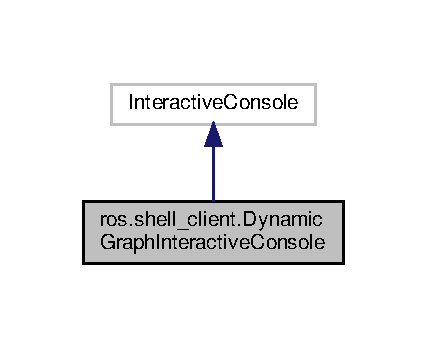
\includegraphics[width=205pt]{classros_1_1shell__client_1_1DynamicGraphInteractiveConsole__inherit__graph}
\end{center}
\end{figure}


Collaboration diagram for ros.\+shell\+\_\+client.\+Dynamic\+Graph\+Interactive\+Console\+:
\nopagebreak
\begin{figure}[H]
\begin{center}
\leavevmode
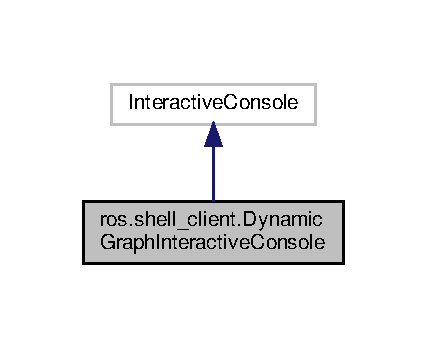
\includegraphics[width=205pt]{classros_1_1shell__client_1_1DynamicGraphInteractiveConsole__coll__graph}
\end{center}
\end{figure}
\subsection*{Public Member Functions}
\begin{DoxyCompactItemize}
\item 
\mbox{\Hypertarget{classros_1_1shell__client_1_1DynamicGraphInteractiveConsole_a55c1e79124ad87114bd27c5f1b7550bf}\label{classros_1_1shell__client_1_1DynamicGraphInteractiveConsole_a55c1e79124ad87114bd27c5f1b7550bf}} 
def {\bfseries \+\_\+\+\_\+init\+\_\+\+\_\+} (self)
\item 
def \hyperlink{classros_1_1shell__client_1_1DynamicGraphInteractiveConsole_ae2781aac94d439abbdc158961562342f}{runcode} (self, code)
\begin{DoxyCompactList}\small\item\em Inherited from code.\+Interactive\+Console. \end{DoxyCompactList}\item 
def \hyperlink{classros_1_1shell__client_1_1DynamicGraphInteractiveConsole_afe6b432e407d107434ccc105a99f7746}{runsource} (self, source, filename=\textquotesingle{}$<$ input $>$\textquotesingle{}, symbol=\textquotesingle{}single\textquotesingle{})
\begin{DoxyCompactList}\small\item\em Inherited from code.\+Interactive\+Console. \end{DoxyCompactList}\item 
\mbox{\Hypertarget{classros_1_1shell__client_1_1DynamicGraphInteractiveConsole_aa7e3a07d2def8b5266cb5925bb049d9f}\label{classros_1_1shell__client_1_1DynamicGraphInteractiveConsole_aa7e3a07d2def8b5266cb5925bb049d9f}} 
def {\bfseries push} (self, line)
\end{DoxyCompactItemize}
\subsection*{Public Attributes}
\begin{DoxyCompactItemize}
\item 
\mbox{\Hypertarget{classros_1_1shell__client_1_1DynamicGraphInteractiveConsole_a77621fd2201b8806aa151e249246e47a}\label{classros_1_1shell__client_1_1DynamicGraphInteractiveConsole_a77621fd2201b8806aa151e249246e47a}} 
{\bfseries lined\+\_\+pushed}
\item 
\mbox{\Hypertarget{classros_1_1shell__client_1_1DynamicGraphInteractiveConsole_ad84d4c48a16b1fe47a923a02acdd41c3}\label{classros_1_1shell__client_1_1DynamicGraphInteractiveConsole_ad84d4c48a16b1fe47a923a02acdd41c3}} 
{\bfseries ros\+\_\+python\+\_\+interpreter}
\end{DoxyCompactItemize}


\subsection{Detailed Description}
For the subtilities please read \href{https://docs.python.org/3/library/code.html}{\tt https\+://docs.\+python.\+org/3/library/code.\+html}. 

\subsection{Member Function Documentation}
\mbox{\Hypertarget{classros_1_1shell__client_1_1DynamicGraphInteractiveConsole_ae2781aac94d439abbdc158961562342f}\label{classros_1_1shell__client_1_1DynamicGraphInteractiveConsole_ae2781aac94d439abbdc158961562342f}} 
\index{ros\+::shell\+\_\+client\+::\+Dynamic\+Graph\+Interactive\+Console@{ros\+::shell\+\_\+client\+::\+Dynamic\+Graph\+Interactive\+Console}!runcode@{runcode}}
\index{runcode@{runcode}!ros\+::shell\+\_\+client\+::\+Dynamic\+Graph\+Interactive\+Console@{ros\+::shell\+\_\+client\+::\+Dynamic\+Graph\+Interactive\+Console}}
\subsubsection{\texorpdfstring{runcode()}{runcode()}}
{\footnotesize\ttfamily def ros.\+shell\+\_\+client.\+Dynamic\+Graph\+Interactive\+Console.\+runcode (\begin{DoxyParamCaption}\item[{}]{self,  }\item[{}]{code }\end{DoxyParamCaption})}



Inherited from code.\+Interactive\+Console. 

We execute the code pushed in the cache {\ttfamily self.\+lined\+\_\+pushed}. The code is pushed whenever the user press enter during the interactive session. see \href{https://docs.python.org/3/library/code.html}{\tt https\+://docs.\+python.\+org/3/library/code.\+html} \mbox{\Hypertarget{classros_1_1shell__client_1_1DynamicGraphInteractiveConsole_afe6b432e407d107434ccc105a99f7746}\label{classros_1_1shell__client_1_1DynamicGraphInteractiveConsole_afe6b432e407d107434ccc105a99f7746}} 
\index{ros\+::shell\+\_\+client\+::\+Dynamic\+Graph\+Interactive\+Console@{ros\+::shell\+\_\+client\+::\+Dynamic\+Graph\+Interactive\+Console}!runsource@{runsource}}
\index{runsource@{runsource}!ros\+::shell\+\_\+client\+::\+Dynamic\+Graph\+Interactive\+Console@{ros\+::shell\+\_\+client\+::\+Dynamic\+Graph\+Interactive\+Console}}
\subsubsection{\texorpdfstring{runsource()}{runsource()}}
{\footnotesize\ttfamily def ros.\+shell\+\_\+client.\+Dynamic\+Graph\+Interactive\+Console.\+runsource (\begin{DoxyParamCaption}\item[{}]{self,  }\item[{}]{source,  }\item[{}]{filename = {\ttfamily \textquotesingle{}$<$input$>$\textquotesingle{}},  }\item[{}]{symbol = {\ttfamily \textquotesingle{}single\textquotesingle{}} }\end{DoxyParamCaption})}



Inherited from code.\+Interactive\+Console. 

see \href{https://docs.python.org/3/library/code.html}{\tt https\+://docs.\+python.\+org/3/library/code.\+html} 

The documentation for this class was generated from the following file\+:\begin{DoxyCompactItemize}
\item 
python/dynamic\+\_\+graph\+\_\+manager/ros/\hyperlink{shell__client_8py}{shell\+\_\+client.\+py}\end{DoxyCompactItemize}

\hypertarget{classros__nodes_1_1run__command_1_1DynamicGraphInteractiveConsole}{}\section{ros\+\_\+nodes.\+run\+\_\+command.\+Dynamic\+Graph\+Interactive\+Console Class Reference}
\label{classros__nodes_1_1run__command_1_1DynamicGraphInteractiveConsole}\index{ros\+\_\+nodes.\+run\+\_\+command.\+Dynamic\+Graph\+Interactive\+Console@{ros\+\_\+nodes.\+run\+\_\+command.\+Dynamic\+Graph\+Interactive\+Console}}


For the subtilities please read \href{https://docs.python.org/3/library/code.html}{\tt https\+://docs.\+python.\+org/3/library/code.\+html}.  




Inheritance diagram for ros\+\_\+nodes.\+run\+\_\+command.\+Dynamic\+Graph\+Interactive\+Console\+:
\nopagebreak
\begin{figure}[H]
\begin{center}
\leavevmode
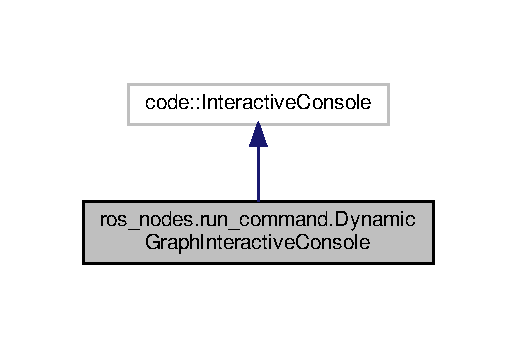
\includegraphics[width=248pt]{classros__nodes_1_1run__command_1_1DynamicGraphInteractiveConsole__inherit__graph}
\end{center}
\end{figure}


Collaboration diagram for ros\+\_\+nodes.\+run\+\_\+command.\+Dynamic\+Graph\+Interactive\+Console\+:
\nopagebreak
\begin{figure}[H]
\begin{center}
\leavevmode
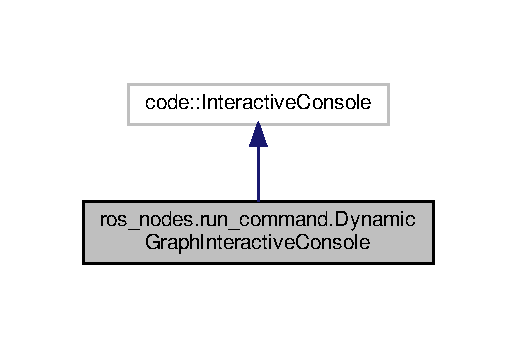
\includegraphics[width=248pt]{classros__nodes_1_1run__command_1_1DynamicGraphInteractiveConsole__coll__graph}
\end{center}
\end{figure}
\subsection*{Public Member Functions}
\begin{DoxyCompactItemize}
\item 
def {\bfseries \+\_\+\+\_\+init\+\_\+\+\_\+} (self)\hypertarget{classros__nodes_1_1run__command_1_1DynamicGraphInteractiveConsole_a07b741ddfb4d749aca2d5ffe9e600b3d}{}\label{classros__nodes_1_1run__command_1_1DynamicGraphInteractiveConsole_a07b741ddfb4d749aca2d5ffe9e600b3d}

\item 
def \hyperlink{classros__nodes_1_1run__command_1_1DynamicGraphInteractiveConsole_a2ef2227d691887e3dd6675c0df5acc2c}{runcode} (self, code)
\begin{DoxyCompactList}\small\item\em Inherited from code.\+Interactive\+Console. \end{DoxyCompactList}\item 
def \hyperlink{classros__nodes_1_1run__command_1_1DynamicGraphInteractiveConsole_a20a3fd5163e9cd015837fde8e6cead02}{runsource} (self, source, filename=\textquotesingle{}$<$ input $>$\textquotesingle{}, symbol=\textquotesingle{}single\textquotesingle{})
\begin{DoxyCompactList}\small\item\em Inherited from code.\+Interactive\+Console. \end{DoxyCompactList}\item 
def {\bfseries push} (self, line)\hypertarget{classros__nodes_1_1run__command_1_1DynamicGraphInteractiveConsole_abf532b80ab37a9938e353e98e9a5c5a7}{}\label{classros__nodes_1_1run__command_1_1DynamicGraphInteractiveConsole_abf532b80ab37a9938e353e98e9a5c5a7}

\end{DoxyCompactItemize}
\subsection*{Public Attributes}
\begin{DoxyCompactItemize}
\item 
{\bfseries lines\+\_\+pushed}\hypertarget{classros__nodes_1_1run__command_1_1DynamicGraphInteractiveConsole_a1d64acd7b772889fc847983bfefc5a79}{}\label{classros__nodes_1_1run__command_1_1DynamicGraphInteractiveConsole_a1d64acd7b772889fc847983bfefc5a79}

\item 
{\bfseries ros\+\_\+python\+\_\+interpreter}\hypertarget{classros__nodes_1_1run__command_1_1DynamicGraphInteractiveConsole_a50579867ed5087f14bf681356cdcf914}{}\label{classros__nodes_1_1run__command_1_1DynamicGraphInteractiveConsole_a50579867ed5087f14bf681356cdcf914}

\end{DoxyCompactItemize}


\subsection{Detailed Description}
For the subtilities please read \href{https://docs.python.org/3/library/code.html}{\tt https\+://docs.\+python.\+org/3/library/code.\+html}. 

\subsection{Member Function Documentation}
\index{ros\+\_\+nodes\+::run\+\_\+command\+::\+Dynamic\+Graph\+Interactive\+Console@{ros\+\_\+nodes\+::run\+\_\+command\+::\+Dynamic\+Graph\+Interactive\+Console}!runcode@{runcode}}
\index{runcode@{runcode}!ros\+\_\+nodes\+::run\+\_\+command\+::\+Dynamic\+Graph\+Interactive\+Console@{ros\+\_\+nodes\+::run\+\_\+command\+::\+Dynamic\+Graph\+Interactive\+Console}}
\subsubsection[{\texorpdfstring{runcode(self, code)}{runcode(self, code)}}]{\setlength{\rightskip}{0pt plus 5cm}def ros\+\_\+nodes.\+run\+\_\+command.\+Dynamic\+Graph\+Interactive\+Console.\+runcode (
\begin{DoxyParamCaption}
\item[{}]{self, }
\item[{}]{code}
\end{DoxyParamCaption}
)}\hypertarget{classros__nodes_1_1run__command_1_1DynamicGraphInteractiveConsole_a2ef2227d691887e3dd6675c0df5acc2c}{}\label{classros__nodes_1_1run__command_1_1DynamicGraphInteractiveConsole_a2ef2227d691887e3dd6675c0df5acc2c}


Inherited from code.\+Interactive\+Console. 

We execute the code pushed in the cache {\ttfamily self.\+lines\+\_\+pushed}. The code is pushed whenever the user press enter during the interactive session. see \href{https://docs.python.org/3/library/code.html}{\tt https\+://docs.\+python.\+org/3/library/code.\+html} \index{ros\+\_\+nodes\+::run\+\_\+command\+::\+Dynamic\+Graph\+Interactive\+Console@{ros\+\_\+nodes\+::run\+\_\+command\+::\+Dynamic\+Graph\+Interactive\+Console}!runsource@{runsource}}
\index{runsource@{runsource}!ros\+\_\+nodes\+::run\+\_\+command\+::\+Dynamic\+Graph\+Interactive\+Console@{ros\+\_\+nodes\+::run\+\_\+command\+::\+Dynamic\+Graph\+Interactive\+Console}}
\subsubsection[{\texorpdfstring{runsource(self, source, filename=\textquotesingle{}$<$ input $>$\textquotesingle{}, symbol=\textquotesingle{}single\textquotesingle{})}{runsource(self, source, filename='< input >', symbol='single')}}]{\setlength{\rightskip}{0pt plus 5cm}def ros\+\_\+nodes.\+run\+\_\+command.\+Dynamic\+Graph\+Interactive\+Console.\+runsource (
\begin{DoxyParamCaption}
\item[{}]{self, }
\item[{}]{source, }
\item[{}]{filename = {\ttfamily \textquotesingle{}$<$input$>$\textquotesingle{}}, }
\item[{}]{symbol = {\ttfamily \textquotesingle{}single\textquotesingle{}}}
\end{DoxyParamCaption}
)}\hypertarget{classros__nodes_1_1run__command_1_1DynamicGraphInteractiveConsole_a20a3fd5163e9cd015837fde8e6cead02}{}\label{classros__nodes_1_1run__command_1_1DynamicGraphInteractiveConsole_a20a3fd5163e9cd015837fde8e6cead02}


Inherited from code.\+Interactive\+Console. 

see \href{https://docs.python.org/3/library/code.html}{\tt https\+://docs.\+python.\+org/3/library/code.\+html} 

The documentation for this class was generated from the following file\+:\begin{DoxyCompactItemize}
\item 
python/ros\+\_\+nodes/\hyperlink{run__command_8py}{run\+\_\+command.\+py}\end{DoxyCompactItemize}

\hypertarget{classdynamic__graph_1_1DynamicGraphManager}{}\section{dynamic\+\_\+graph\+:\+:Dynamic\+Graph\+Manager Class Reference}
\label{classdynamic__graph_1_1DynamicGraphManager}\index{dynamic\+\_\+graph\+::\+Dynamic\+Graph\+Manager@{dynamic\+\_\+graph\+::\+Dynamic\+Graph\+Manager}}


This class has for purpose to manage the different processes during run time.  




{\ttfamily \#include $<$dynamic\+\_\+graph\+\_\+manager.\+hh$>$}



Inheritance diagram for dynamic\+\_\+graph\+:\+:Dynamic\+Graph\+Manager\+:
\nopagebreak
\begin{figure}[H]
\begin{center}
\leavevmode
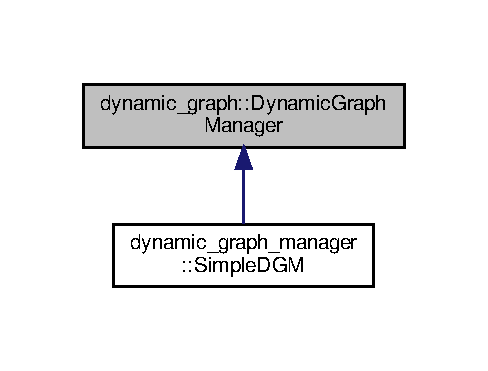
\includegraphics[width=234pt]{classdynamic__graph_1_1DynamicGraphManager__inherit__graph}
\end{center}
\end{figure}
\subsection*{Public Member Functions}
\begin{DoxyCompactItemize}
\item 
\hyperlink{classdynamic__graph_1_1DynamicGraphManager_afd98424082e5a1f878e6c7cb08a62c4a}{Dynamic\+Graph\+Manager} ()\hypertarget{classdynamic__graph_1_1DynamicGraphManager_afd98424082e5a1f878e6c7cb08a62c4a}{}\label{classdynamic__graph_1_1DynamicGraphManager_afd98424082e5a1f878e6c7cb08a62c4a}

\begin{DoxyCompactList}\small\item\em \hyperlink{classdynamic__graph_1_1DynamicGraphManager}{Dynamic\+Graph\+Manager}, constructor of the class. \end{DoxyCompactList}\item 
virtual \hyperlink{classdynamic__graph_1_1DynamicGraphManager_a6bcf93d16574035ee654289274d0a790}{$\sim$\+Dynamic\+Graph\+Manager} ()\hypertarget{classdynamic__graph_1_1DynamicGraphManager_a6bcf93d16574035ee654289274d0a790}{}\label{classdynamic__graph_1_1DynamicGraphManager_a6bcf93d16574035ee654289274d0a790}

\begin{DoxyCompactList}\small\item\em \hyperlink{classdynamic__graph_1_1DynamicGraphManager}{Dynamic\+Graph\+Manager}, destructor of the class. \end{DoxyCompactList}\item 
void \hyperlink{classdynamic__graph_1_1DynamicGraphManager_ac6859456bbdd4307cb880dc5e54131dd}{initialize} (Y\+A\+M\+L\+::\+Node param)\hypertarget{classdynamic__graph_1_1DynamicGraphManager_ac6859456bbdd4307cb880dc5e54131dd}{}\label{classdynamic__graph_1_1DynamicGraphManager_ac6859456bbdd4307cb880dc5e54131dd}

\begin{DoxyCompactList}\small\item\em initialize the basic variables \end{DoxyCompactList}\item 
void \hyperlink{classdynamic__graph_1_1DynamicGraphManager_a93272fcbb3793dfc92422186022ecf72}{run} ()
\begin{DoxyCompactList}\small\item\em \hyperlink{classdynamic__graph_1_1DynamicGraphManager_a93272fcbb3793dfc92422186022ecf72}{run()} splits the process in the \hyperlink{namespacedynamic__graph}{dynamic\+\_\+graph} process and the hadware\+\_\+communication process. \end{DoxyCompactList}\item 
void \hyperlink{classdynamic__graph_1_1DynamicGraphManager_a18dab9ca9c8901779a944386f2b8898c}{wait\+\_\+start\+\_\+dynamic\+\_\+graph} ()\hypertarget{classdynamic__graph_1_1DynamicGraphManager_a18dab9ca9c8901779a944386f2b8898c}{}\label{classdynamic__graph_1_1DynamicGraphManager_a18dab9ca9c8901779a944386f2b8898c}

\begin{DoxyCompactList}\small\item\em wait\+\_\+start\+\_\+dynamic\+\_\+graph put the current thread to sleep until the user start the dynamic graph \end{DoxyCompactList}\item 
void \hyperlink{classdynamic__graph_1_1DynamicGraphManager_ab827a776b4ac31ea91ace9a2bfc1e99d}{wait\+\_\+stop\+\_\+dynamic\+\_\+graph} ()\hypertarget{classdynamic__graph_1_1DynamicGraphManager_ab827a776b4ac31ea91ace9a2bfc1e99d}{}\label{classdynamic__graph_1_1DynamicGraphManager_ab827a776b4ac31ea91ace9a2bfc1e99d}

\begin{DoxyCompactList}\small\item\em wait\+\_\+stop\+\_\+dynamic\+\_\+graph put the current thread to sleep until the user stop the dynamic graph \end{DoxyCompactList}\item 
void \hyperlink{classdynamic__graph_1_1DynamicGraphManager_a83a98e169cd587d101bba69bb799e408}{wait\+\_\+stop\+\_\+hardware\+\_\+communication} ()
\begin{DoxyCompactList}\small\item\em wait\+\_\+stop\+\_\+hardware\+\_\+communication put the current thread to sleep until the user stop the hardware communication. \end{DoxyCompactList}\item 
void \hyperlink{classdynamic__graph_1_1DynamicGraphManager_a81926d5d33573d667bc6511bbb2d8f52}{initialize\+\_\+dynamic\+\_\+graph\+\_\+process} ()\hypertarget{classdynamic__graph_1_1DynamicGraphManager_a81926d5d33573d667bc6511bbb2d8f52}{}\label{classdynamic__graph_1_1DynamicGraphManager_a81926d5d33573d667bc6511bbb2d8f52}

\begin{DoxyCompactList}\small\item\em initialize\+\_\+dynamic\+\_\+graph\+\_\+process instanciates all variables related to the \hyperlink{namespacedynamic__graph}{dynamic\+\_\+graph} and user interface. \end{DoxyCompactList}\item 
void \hyperlink{classdynamic__graph_1_1DynamicGraphManager_a56acce72235fe0786830ec19a3439309}{run\+\_\+python\+\_\+command} (std\+::ostream \&file, const std\+::string \&command)
\begin{DoxyCompactList}\small\item\em run\+\_\+python\+\_\+command \end{DoxyCompactList}\item 
void \hyperlink{classdynamic__graph_1_1DynamicGraphManager_a11cc3b7fefc7fe146dc112a7e6d55f3d}{python\+\_\+prologue} ()\hypertarget{classdynamic__graph_1_1DynamicGraphManager_a11cc3b7fefc7fe146dc112a7e6d55f3d}{}\label{classdynamic__graph_1_1DynamicGraphManager_a11cc3b7fefc7fe146dc112a7e6d55f3d}

\begin{DoxyCompactList}\small\item\em python\+\_\+prologue get the pointer of the device in the the python interpretor. \end{DoxyCompactList}\item 
virtual void \hyperlink{classdynamic__graph_1_1DynamicGraphManager_a8e23eb4ce0acaef397bf84a770b9f015}{run\+\_\+dynamic\+\_\+graph\+\_\+process} ()
\begin{DoxyCompactList}\small\item\em run\+\_\+dynamic\+\_\+graph\+\_\+process spawns the real time thread and becomes a ros spinner (thread in charge of the ros\+::service callbacks). \end{DoxyCompactList}\item 
virtual void \hyperlink{classdynamic__graph_1_1DynamicGraphManager_a81e7cb10262383030c10156730d39ce8}{run\+\_\+hardware\+\_\+communication\+\_\+process} ()
\begin{DoxyCompactList}\small\item\em run\+\_\+hardware\+\_\+communication\+\_\+process spawns the real time thread. \end{DoxyCompactList}\item 
virtual void \hyperlink{classdynamic__graph_1_1DynamicGraphManager_ad13f5aef302173293a0c162c28505ef8}{run\+\_\+single\+\_\+process} ()
\begin{DoxyCompactList}\small\item\em run\+\_\+single\+\_\+process spawns the real time thread. \end{DoxyCompactList}\item 
virtual void \hyperlink{classdynamic__graph_1_1DynamicGraphManager_ae3927887762c52c7bf50ab5a565c3077}{initialize\+\_\+hardware\+\_\+communication\+\_\+process} ()
\begin{DoxyCompactList}\small\item\em initialize\+\_\+hardware\+\_\+communication\+\_\+process instanciate all variables related to the hardware communication. \end{DoxyCompactList}\item 
virtual void \hyperlink{classdynamic__graph_1_1DynamicGraphManager_a7bddce83d5185433041ad27610b85b3a}{get\+\_\+sensors\+\_\+to\+\_\+map} (\hyperlink{namespacedynamic__graph_a51212ed7fa4ae81e7b362a27f09b7ab8}{Vector\+D\+G\+Map} \&)
\begin{DoxyCompactList}\small\item\em get\+\_\+sensors\+\_\+to\+\_\+map is the fonction that get the motor command from a map and that uses the drivers to send these command to the robot. \end{DoxyCompactList}\item 
virtual void \hyperlink{classdynamic__graph_1_1DynamicGraphManager_a506e6f37ac7205efaf0efe4202cde897}{set\+\_\+motor\+\_\+controls\+\_\+from\+\_\+map} (const \hyperlink{namespacedynamic__graph_a51212ed7fa4ae81e7b362a27f09b7ab8}{Vector\+D\+G\+Map} \&)
\begin{DoxyCompactList}\small\item\em set\+\_\+motor\+\_\+controls\+\_\+from\+\_\+map is the fonction that get the motor command from a map and that uses the drivers to send these command to the robot. \end{DoxyCompactList}\item 
virtual void \hyperlink{classdynamic__graph_1_1DynamicGraphManager_a60bb31040121d6041b4dd6556f5c7eac}{compute\+\_\+safety\+\_\+controls} ()\hypertarget{classdynamic__graph_1_1DynamicGraphManager_a60bb31040121d6041b4dd6556f5c7eac}{}\label{classdynamic__graph_1_1DynamicGraphManager_a60bb31040121d6041b4dd6556f5c7eac}

\begin{DoxyCompactList}\small\item\em compute\+\_\+safety\+\_\+controls computes safety controls very fast in case the dynamic graph is taking to much computation time or has crashed. \end{DoxyCompactList}\item 
void \hyperlink{classdynamic__graph_1_1DynamicGraphManager_ad3c7c528ef283fbfb803377c8c631b4c}{stop\+\_\+dynamic\+\_\+graph} ()
\begin{DoxyCompactList}\small\item\em stop\+\_\+dynamic\+\_\+graph stop the Dynamic\+Graph. \end{DoxyCompactList}\item 
void \hyperlink{classdynamic__graph_1_1DynamicGraphManager_a1bfd2b965dde19d12d63f5928a4f670c}{start\+\_\+dynamic\+\_\+graph} ()
\begin{DoxyCompactList}\small\item\em start\+\_\+dynamic\+\_\+graph start the Dynamic\+Graph. \end{DoxyCompactList}\item 
bool \hyperlink{classdynamic__graph_1_1DynamicGraphManager_ab929d21277e5d2fba726b8ae422c27a8}{is\+\_\+dynamic\+\_\+graph\+\_\+stopped} ()
\begin{DoxyCompactList}\small\item\em get the status of the dynamic graph (is running or not) \end{DoxyCompactList}\item 
void \hyperlink{classdynamic__graph_1_1DynamicGraphManager_aabf11778fb69e5203d38c8093de60bab}{stop\+\_\+hardware\+\_\+communication} ()
\begin{DoxyCompactList}\small\item\em stop\+\_\+hardware\+\_\+communication stops the hardware communication. \end{DoxyCompactList}\item 
void \hyperlink{classdynamic__graph_1_1DynamicGraphManager_a234bef10fea6e3f9beb1580491127660}{start\+\_\+hardware\+\_\+communication} ()
\begin{DoxyCompactList}\small\item\em start\+\_\+hardware\+\_\+communication starts the hardware communication. \end{DoxyCompactList}\item 
bool \hyperlink{classdynamic__graph_1_1DynamicGraphManager_afcc53ebec6e5f2057c23a05894715125}{is\+\_\+hardware\+\_\+communication\+\_\+stopped} ()
\begin{DoxyCompactList}\small\item\em get the status of the hardware communication (is running or not). \end{DoxyCompactList}\item 
pid\+\_\+t \hyperlink{classdynamic__graph_1_1DynamicGraphManager_a9c11927e0b76e91fabc4b34ea7fb85bc}{pid\+\_\+dynamic\+\_\+graph\+\_\+process} ()
\begin{DoxyCompactList}\small\item\em pid\+\_\+dynamic\+\_\+graph\+\_\+process is an accessor on the pid of the process \end{DoxyCompactList}\item 
pid\+\_\+t \hyperlink{classdynamic__graph_1_1DynamicGraphManager_ac1abb11591e037e203329e900c89f4f5}{pid\+\_\+hardware\+\_\+communication\+\_\+process} ()
\begin{DoxyCompactList}\small\item\em pid\+\_\+hardware\+\_\+communication\+\_\+process is an accessor on the pid of the process \end{DoxyCompactList}\item 
\hyperlink{classdynamic__graph_1_1Device}{Device} \& \hyperlink{classdynamic__graph_1_1DynamicGraphManager_a90bb14375da3d2aaaeafb356b6ca54f7}{device} ()
\begin{DoxyCompactList}\small\item\em device is a getter method on the \hyperlink{classdynamic__graph_1_1Device}{Device} internal pointer. \end{DoxyCompactList}\item 
bool \hyperlink{classdynamic__graph_1_1DynamicGraphManager_ab980a2384c817ab5f59e712a54b2261a}{has\+\_\+dynamic\+\_\+graph\+\_\+process\+\_\+died} ()
\begin{DoxyCompactList}\small\item\em has\+\_\+dynamic\+\_\+graph\+\_\+process\+\_\+died check if the process of the Dynamic\+Graph has died or not. \end{DoxyCompactList}\item 
virtual bool \hyperlink{classdynamic__graph_1_1DynamicGraphManager_aea29e8dc351e0a50a8d2803d854d238d}{is\+\_\+in\+\_\+safety\+\_\+mode} ()
\begin{DoxyCompactList}\small\item\em is\+\_\+in\+\_\+safety\+\_\+mode check if the dynamic graph is still alive and sending commands at a descent frequency. \end{DoxyCompactList}\end{DoxyCompactItemize}
\subsection*{Static Public Attributes}
\begin{DoxyCompactItemize}
\item 
static const std\+::string \hyperlink{classdynamic__graph_1_1DynamicGraphManager_a391d7a3f7c3df820d31f2c1d0ff7fc51}{dg\+\_\+ros\+\_\+node\+\_\+name\+\_\+} = \char`\"{}dynamic\+\_\+graph\char`\"{}\hypertarget{classdynamic__graph_1_1DynamicGraphManager_a391d7a3f7c3df820d31f2c1d0ff7fc51}{}\label{classdynamic__graph_1_1DynamicGraphManager_a391d7a3f7c3df820d31f2c1d0ff7fc51}

\begin{DoxyCompactList}\small\item\em dg\+\_\+ros\+\_\+node\+\_\+name\+\_\+ this is the ros node name of the dynamic graph process \end{DoxyCompactList}\item 
static const std\+::string \hyperlink{classdynamic__graph_1_1DynamicGraphManager_a415f24927dbe9dfd0ee4a6462428bd48}{hw\+\_\+com\+\_\+ros\+\_\+node\+\_\+name\+\_\+}
\begin{DoxyCompactList}\small\item\em hw\+\_\+com\+\_\+ros\+\_\+node\+\_\+name\+\_\+ this is the ros node name of the harware communication process \end{DoxyCompactList}\item 
static const std\+::string \hyperlink{classdynamic__graph_1_1DynamicGraphManager_a97fa7b0a31efa6192c3dcc44fbe63886}{shared\+\_\+memory\+\_\+name\+\_\+} = \char`\"{}D\+G\+M\+\_\+\+ShM\char`\"{}\hypertarget{classdynamic__graph_1_1DynamicGraphManager_a97fa7b0a31efa6192c3dcc44fbe63886}{}\label{classdynamic__graph_1_1DynamicGraphManager_a97fa7b0a31efa6192c3dcc44fbe63886}

\begin{DoxyCompactList}\small\item\em shared\+\_\+memory\+\_\+name is the name of the shared memory segment to be used \end{DoxyCompactList}\item 
static const std\+::string \hyperlink{classdynamic__graph_1_1DynamicGraphManager_abd4e4f618fbdacfda8c2cdece08e401b}{sensors\+\_\+map\+\_\+name\+\_\+} = \char`\"{}sensors\+\_\+map\char`\"{}\hypertarget{classdynamic__graph_1_1DynamicGraphManager_abd4e4f618fbdacfda8c2cdece08e401b}{}\label{classdynamic__graph_1_1DynamicGraphManager_abd4e4f618fbdacfda8c2cdece08e401b}

\begin{DoxyCompactList}\small\item\em sensors\+\_\+map\+\_\+name is the name of the sensor map inside the shared memory segment \end{DoxyCompactList}\item 
static const std\+::string \hyperlink{classdynamic__graph_1_1DynamicGraphManager_a056de4d7a49496b2b0812d96d93370d9}{motor\+\_\+controls\+\_\+map\+\_\+name\+\_\+}
\begin{DoxyCompactList}\small\item\em motor\+\_\+controls\+\_\+map\+\_\+name is the name of the motor controls map inside the shared memory segment \end{DoxyCompactList}\item 
static const std\+::string \hyperlink{classdynamic__graph_1_1DynamicGraphManager_a909b8d2d024a2a11473fa2d94a18002e}{cond\+\_\+var\+\_\+name\+\_\+} = \char`\"{}cond\+\_\+var\char`\"{}\hypertarget{classdynamic__graph_1_1DynamicGraphManager_a909b8d2d024a2a11473fa2d94a18002e}{}\label{classdynamic__graph_1_1DynamicGraphManager_a909b8d2d024a2a11473fa2d94a18002e}

\begin{DoxyCompactList}\small\item\em cond\+\_\+var\+\_\+sensors\+\_\+name\+\_\+ is the name of the condition variable in the shared memory \end{DoxyCompactList}\end{DoxyCompactItemize}
\subsection*{Protected Member Functions}
\begin{DoxyCompactItemize}
\item 
void \hyperlink{classdynamic__graph_1_1DynamicGraphManager_a72146c4ddd173869a512e9f174ad48df}{add\+\_\+user\+\_\+command} (std\+::function$<$ void(void)$>$ func)
\begin{DoxyCompactList}\small\item\em Method inherited. \end{DoxyCompactList}\end{DoxyCompactItemize}
\subsection*{Protected Attributes}
\begin{DoxyCompactItemize}
\item 
ros\+::\+Service\+Server \hyperlink{classdynamic__graph_1_1DynamicGraphManager_adb99ba3a7a5e677b30531a69bcc922ec}{ros\+\_\+service\+\_\+start\+\_\+dg\+\_\+}
\begin{DoxyCompactList}\small\item\em ros\+\_\+service\+\_\+start\+\_\+dg\+\_\+ allows to start the dynamic graph on call. \end{DoxyCompactList}\item 
ros\+::\+Service\+Server \hyperlink{classdynamic__graph_1_1DynamicGraphManager_adf973b6da4e4fe14cae262ba94ebb191}{ros\+\_\+service\+\_\+stop\+\_\+dg\+\_\+}
\begin{DoxyCompactList}\small\item\em ros\+\_\+service\+\_\+stop\+\_\+dg\+\_\+ allows to stop the dynamic graph on call. \end{DoxyCompactList}\item 
std\+::atomic$<$ bool $>$ \hyperlink{classdynamic__graph_1_1DynamicGraphManager_a87baafbaadf396a7663da653dc5da106}{is\+\_\+dynamic\+\_\+graph\+\_\+stopped\+\_\+}
\begin{DoxyCompactList}\small\item\em is\+\_\+dynamic\+\_\+graph\+\_\+stopped\+\_\+ is the flag reflecting the state of the dynamic graph. \end{DoxyCompactList}\item 
std\+::atomic$<$ bool $>$ \hyperlink{classdynamic__graph_1_1DynamicGraphManager_ab1a2bc0a8f04126638056f430297097e}{is\+\_\+hardware\+\_\+communication\+\_\+stopped\+\_\+}
\begin{DoxyCompactList}\small\item\em is\+\_\+hardware\+\_\+communication\+\_\+stopped\+\_\+ is the flag reflecting the state of the hardware communication thread. \end{DoxyCompactList}\item 
std\+::unique\+\_\+ptr$<$ \hyperlink{classdynamic__graph_1_1RosPythonInterpreter}{dynamic\+\_\+graph\+::\+Ros\+Python\+Interpreter} $>$ \hyperlink{classdynamic__graph_1_1DynamicGraphManager_a40458dd801d1ee7e2051f8b8fab5366b}{ros\+\_\+python\+\_\+interpreter\+\_\+}\hypertarget{classdynamic__graph_1_1DynamicGraphManager_a40458dd801d1ee7e2051f8b8fab5366b}{}\label{classdynamic__graph_1_1DynamicGraphManager_a40458dd801d1ee7e2051f8b8fab5366b}

\begin{DoxyCompactList}\small\item\em ros\+\_\+python\+\_\+interpreter\+\_\+ptr\+\_\+ is a R\+OS wrapper around a python interpreter. \end{DoxyCompactList}\item 
std\+::unique\+\_\+ptr$<$ real\+\_\+time\+\_\+tools\+::\+Real\+Time\+Thread $>$ \hyperlink{classdynamic__graph_1_1DynamicGraphManager_aee7d35de31cdb05958c1b4f539c290ae}{thread\+\_\+dynamic\+\_\+graph\+\_\+}\hypertarget{classdynamic__graph_1_1DynamicGraphManager_aee7d35de31cdb05958c1b4f539c290ae}{}\label{classdynamic__graph_1_1DynamicGraphManager_aee7d35de31cdb05958c1b4f539c290ae}

\begin{DoxyCompactList}\small\item\em thread\+\_\+dynamic\+\_\+graph\+\_\+ is the real time thread that runs the dynamic graph. \end{DoxyCompactList}\item 
std\+::unique\+\_\+ptr$<$ real\+\_\+time\+\_\+tools\+::\+Real\+Time\+Thread $>$ \hyperlink{classdynamic__graph_1_1DynamicGraphManager_ae0e1a3c59fa7d0282529e1a544e83b4d}{thread\+\_\+hardware\+\_\+communication\+\_\+}\hypertarget{classdynamic__graph_1_1DynamicGraphManager_ae0e1a3c59fa7d0282529e1a544e83b4d}{}\label{classdynamic__graph_1_1DynamicGraphManager_ae0e1a3c59fa7d0282529e1a544e83b4d}

\begin{DoxyCompactList}\small\item\em thread\+\_\+hardware\+\_\+communication\+\_\+ is the real thread that communicate with the hardware. \end{DoxyCompactList}\item 
pid\+\_\+t \hyperlink{classdynamic__graph_1_1DynamicGraphManager_aa8aa645099e7e9cce426381e38b5027d}{pid\+\_\+dynamic\+\_\+graph\+\_\+process\+\_\+}
\begin{DoxyCompactList}\small\item\em pid\+\_\+dynamic\+\_\+graph\+\_\+process\+\_\+ is the pid of the Dynamic\+Graph process. \end{DoxyCompactList}\item 
pid\+\_\+t \hyperlink{classdynamic__graph_1_1DynamicGraphManager_a02232cdc5cabca34d07dada6ced38532}{pid\+\_\+hardware\+\_\+communication\+\_\+process\+\_\+}
\begin{DoxyCompactList}\small\item\em pid\+\_\+hardware\+\_\+communication\+\_\+process\+\_\+ is the pid of the hardware communication process. \end{DoxyCompactList}\item 
std\+::unique\+\_\+ptr$<$ \hyperlink{classdynamic__graph_1_1Device}{Device} $>$ \hyperlink{classdynamic__graph_1_1DynamicGraphManager_a416ca1c33660df4f7f74eb29df4c5a58}{device\+\_\+}\hypertarget{classdynamic__graph_1_1DynamicGraphManager_a416ca1c33660df4f7f74eb29df4c5a58}{}\label{classdynamic__graph_1_1DynamicGraphManager_a416ca1c33660df4f7f74eb29df4c5a58}

\begin{DoxyCompactList}\small\item\em device\+\_\+ is the Dynamic\+Graph device that manages the computation of the graph. \end{DoxyCompactList}\item 
\hyperlink{namespacedynamic__graph_a51212ed7fa4ae81e7b362a27f09b7ab8}{Vector\+D\+G\+Map} \hyperlink{classdynamic__graph_1_1DynamicGraphManager_a896bf6cb22d2d88a5a6a307a2e44608e}{sensors\+\_\+map\+\_\+}
\begin{DoxyCompactList}\small\item\em sensors\+\_\+map\+\_\+ is a map of dynamicgraph\+::\+Vector. \end{DoxyCompactList}\item 
\hyperlink{namespacedynamic__graph_a51212ed7fa4ae81e7b362a27f09b7ab8}{Vector\+D\+G\+Map} \hyperlink{classdynamic__graph_1_1DynamicGraphManager_a03eabd2f08990a1dcc1caa652b701020}{motor\+\_\+controls\+\_\+map\+\_\+}
\begin{DoxyCompactList}\small\item\em motor\+\_\+controls\+\_\+map\+\_\+ is a map of dynamicgraph\+::\+Vector. \end{DoxyCompactList}\item 
std\+::unique\+\_\+ptr$<$ shared\+\_\+memory\+::\+Locked\+Condition\+Variable $>$ \hyperlink{classdynamic__graph_1_1DynamicGraphManager_a003d8598839c07a7d81c1afed0ea0b01}{cond\+\_\+var\+\_\+}\hypertarget{classdynamic__graph_1_1DynamicGraphManager_a003d8598839c07a7d81c1afed0ea0b01}{}\label{classdynamic__graph_1_1DynamicGraphManager_a003d8598839c07a7d81c1afed0ea0b01}

\begin{DoxyCompactList}\small\item\em cond\+\_\+var\+\_\+sensors\+\_\+ this condition variable allow the computation of the dynamic graph just after the acquisition of the sensors \end{DoxyCompactList}\item 
bool \hyperlink{classdynamic__graph_1_1DynamicGraphManager_a7e6cc5e58f1accce947f929d233a67fd}{has\+\_\+been\+\_\+waken\+\_\+by\+\_\+dg\+\_\+}\hypertarget{classdynamic__graph_1_1DynamicGraphManager_a7e6cc5e58f1accce947f929d233a67fd}{}\label{classdynamic__graph_1_1DynamicGraphManager_a7e6cc5e58f1accce947f929d233a67fd}

\begin{DoxyCompactList}\small\item\em has\+\_\+been\+\_\+waken\+\_\+by\+\_\+dg\+\_\+ is a flag that indicates if the hardware communication process has been awaken by the \hyperlink{namespacedynamic__graph}{dynamic\+\_\+graph} process or not. \end{DoxyCompactList}\item 
unsigned \hyperlink{classdynamic__graph_1_1DynamicGraphManager_abafc3cf4d8f7dc938f98b7eb07b7af9a}{missed\+\_\+control\+\_\+count\+\_\+}\hypertarget{classdynamic__graph_1_1DynamicGraphManager_abafc3cf4d8f7dc938f98b7eb07b7af9a}{}\label{classdynamic__graph_1_1DynamicGraphManager_abafc3cf4d8f7dc938f98b7eb07b7af9a}

\begin{DoxyCompactList}\small\item\em missed\+\_\+control\+\_\+count\+\_\+ is counting the number of iteration when the \hyperlink{namespacedynamic__graph}{dynamic\+\_\+graph} failed to provide data. \end{DoxyCompactList}\item 
unsigned \hyperlink{classdynamic__graph_1_1DynamicGraphManager_a10922e790e039f78b0fabbb5ef944488}{max\+\_\+missed\+\_\+control\+\_\+}\hypertarget{classdynamic__graph_1_1DynamicGraphManager_a10922e790e039f78b0fabbb5ef944488}{}\label{classdynamic__graph_1_1DynamicGraphManager_a10922e790e039f78b0fabbb5ef944488}

\begin{DoxyCompactList}\small\item\em max\+\_\+missed\+\_\+control\+\_\+ if the missed\+\_\+control\+\_\+count\+\_\+ reach the value of max\+\_\+missed\+\_\+control\+\_\+ then we switch to safety mode. \end{DoxyCompactList}\item 
clock\+::duration \hyperlink{classdynamic__graph_1_1DynamicGraphManager_a1006cdb2d7e30e291d3d568923ebbc03}{control\+\_\+period\+\_\+}\hypertarget{classdynamic__graph_1_1DynamicGraphManager_a1006cdb2d7e30e291d3d568923ebbc03}{}\label{classdynamic__graph_1_1DynamicGraphManager_a1006cdb2d7e30e291d3d568923ebbc03}

\begin{DoxyCompactList}\small\item\em control\+\_\+period\+\_\+ this is the control period in nanoseconds. \end{DoxyCompactList}\item 
clock\+::time\+\_\+point \hyperlink{classdynamic__graph_1_1DynamicGraphManager_a26167d2936575dfdbe31be4717b70cc5}{hw\+\_\+time\+\_\+loop\+\_\+before\+\_\+sleep\+\_\+}\hypertarget{classdynamic__graph_1_1DynamicGraphManager_a26167d2936575dfdbe31be4717b70cc5}{}\label{classdynamic__graph_1_1DynamicGraphManager_a26167d2936575dfdbe31be4717b70cc5}

\begin{DoxyCompactList}\small\item\em hw\+\_\+time\+\_\+loop\+\_\+before\+\_\+sleep\+\_\+ is the time measurement just before the hardware communication loop goes to sleep. \end{DoxyCompactList}\item 
clock\+::time\+\_\+point \hyperlink{classdynamic__graph_1_1DynamicGraphManager_a3641066efdd3424bb2bd745f6ba8d315}{hw\+\_\+time\+\_\+loop\+\_\+after\+\_\+sleep\+\_\+}\hypertarget{classdynamic__graph_1_1DynamicGraphManager_a3641066efdd3424bb2bd745f6ba8d315}{}\label{classdynamic__graph_1_1DynamicGraphManager_a3641066efdd3424bb2bd745f6ba8d315}

\begin{DoxyCompactList}\small\item\em hw\+\_\+time\+\_\+loop\+\_\+after\+\_\+sleep\+\_\+ is the time measurement just after the hardware communication loop goes to sleep. \end{DoxyCompactList}\item 
clock\+::duration \hyperlink{classdynamic__graph_1_1DynamicGraphManager_afb2f9b39e5c529d525999c3e91e06213}{hw\+\_\+meas\+\_\+sleep\+\_\+time\+\_\+}\hypertarget{classdynamic__graph_1_1DynamicGraphManager_afb2f9b39e5c529d525999c3e91e06213}{}\label{classdynamic__graph_1_1DynamicGraphManager_afb2f9b39e5c529d525999c3e91e06213}

\begin{DoxyCompactList}\small\item\em hw\+\_\+measured\+\_\+sleep\+\_\+time\+\_\+ is the time during which the hardware communication process actually slept. \end{DoxyCompactList}\item 
clock\+::duration \hyperlink{classdynamic__graph_1_1DynamicGraphManager_aa89f848a27f201aed320e2c6a441dc02}{hw\+\_\+ref\+\_\+sleep\+\_\+time\+\_\+}\hypertarget{classdynamic__graph_1_1DynamicGraphManager_aa89f848a27f201aed320e2c6a441dc02}{}\label{classdynamic__graph_1_1DynamicGraphManager_aa89f848a27f201aed320e2c6a441dc02}

\begin{DoxyCompactList}\small\item\em hw\+\_\+ref\+\_\+sleep\+\_\+time\+\_\+ is the time during which the hardware communication process is supposed to sleep. \end{DoxyCompactList}\item 
clock\+::duration \hyperlink{classdynamic__graph_1_1DynamicGraphManager_af4c9ca6b9c161ac578b6726eaa7b7826}{hw\+\_\+meas\+\_\+active\+\_\+time\+\_\+}\hypertarget{classdynamic__graph_1_1DynamicGraphManager_af4c9ca6b9c161ac578b6726eaa7b7826}{}\label{classdynamic__graph_1_1DynamicGraphManager_af4c9ca6b9c161ac578b6726eaa7b7826}

\begin{DoxyCompactList}\small\item\em hw\+\_\+meas\+\_\+active\+\_\+time\+\_\+ is the time during which the hardware communication process is supposed to sleep. \end{DoxyCompactList}\item 
bool \hyperlink{classdynamic__graph_1_1DynamicGraphManager_a81617144faf55e4ed2bf60165060b0f5}{is\+\_\+real\+\_\+robot\+\_\+}\hypertarget{classdynamic__graph_1_1DynamicGraphManager_a81617144faf55e4ed2bf60165060b0f5}{}\label{classdynamic__graph_1_1DynamicGraphManager_a81617144faf55e4ed2bf60165060b0f5}

\begin{DoxyCompactList}\small\item\em is\+\_\+real\+\_\+robot this boolean is a parameter to indicate if yes or no we are in simulation or in a real robot mode. \end{DoxyCompactList}\item 
std\+::string \hyperlink{classdynamic__graph_1_1DynamicGraphManager_a18c2cc959dceef659ab1f567e06254f7}{dg\+\_\+active\+\_\+timer\+\_\+file\+\_\+}\hypertarget{classdynamic__graph_1_1DynamicGraphManager_a18c2cc959dceef659ab1f567e06254f7}{}\label{classdynamic__graph_1_1DynamicGraphManager_a18c2cc959dceef659ab1f567e06254f7}

\begin{DoxyCompactList}\small\item\em dg\+\_\+active\+\_\+timer\+\_\+file\+\_\+ this is the path to the file that will contain the computation time of each of the dynamic graph complete execution. \end{DoxyCompactList}\item 
std\+::string \hyperlink{classdynamic__graph_1_1DynamicGraphManager_af02dbc7fb67674937208abe4cd75d652}{dg\+\_\+sleep\+\_\+timer\+\_\+file\+\_\+}\hypertarget{classdynamic__graph_1_1DynamicGraphManager_af02dbc7fb67674937208abe4cd75d652}{}\label{classdynamic__graph_1_1DynamicGraphManager_af02dbc7fb67674937208abe4cd75d652}

\begin{DoxyCompactList}\small\item\em dg\+\_\+sleep\+\_\+timer\+\_\+file\+\_\+ this is the path to the file that will contain the sleep duration of the dynamic graph thread. \end{DoxyCompactList}\item 
std\+::string \hyperlink{classdynamic__graph_1_1DynamicGraphManager_a1a43bcf9c74648466d1e561203a39d87}{dg\+\_\+timer\+\_\+file\+\_\+}\hypertarget{classdynamic__graph_1_1DynamicGraphManager_a1a43bcf9c74648466d1e561203a39d87}{}\label{classdynamic__graph_1_1DynamicGraphManager_a1a43bcf9c74648466d1e561203a39d87}

\begin{DoxyCompactList}\small\item\em dg\+\_\+timer\+\_\+file\+\_\+ this is the path to the file that will contain the time of the dynamic graph loop. \end{DoxyCompactList}\item 
std\+::string \hyperlink{classdynamic__graph_1_1DynamicGraphManager_a2bd29dbd358b8c02805f4df970e75936}{hwc\+\_\+active\+\_\+timer\+\_\+file\+\_\+}\hypertarget{classdynamic__graph_1_1DynamicGraphManager_a2bd29dbd358b8c02805f4df970e75936}{}\label{classdynamic__graph_1_1DynamicGraphManager_a2bd29dbd358b8c02805f4df970e75936}

\begin{DoxyCompactList}\small\item\em hwc\+\_\+active\+\_\+timer\+\_\+file\+\_\+ this is the path to the file that will contain the computation time of each active period of the hardware communication loop. \end{DoxyCompactList}\item 
std\+::string \hyperlink{classdynamic__graph_1_1DynamicGraphManager_a5db6275d202963665a35c5eb2e68088d}{hwc\+\_\+sleep\+\_\+timer\+\_\+file\+\_\+}\hypertarget{classdynamic__graph_1_1DynamicGraphManager_a5db6275d202963665a35c5eb2e68088d}{}\label{classdynamic__graph_1_1DynamicGraphManager_a5db6275d202963665a35c5eb2e68088d}

\begin{DoxyCompactList}\small\item\em hwc\+\_\+sleep\+\_\+timer\+\_\+file\+\_\+ this is the path to the file that will contain the sleeping time of the hardware communication loop. \end{DoxyCompactList}\item 
std\+::string \hyperlink{classdynamic__graph_1_1DynamicGraphManager_a84f97c9eebbecee1af314e74fe22d8ed}{hwc\+\_\+timer\+\_\+file\+\_\+}\hypertarget{classdynamic__graph_1_1DynamicGraphManager_a84f97c9eebbecee1af314e74fe22d8ed}{}\label{classdynamic__graph_1_1DynamicGraphManager_a84f97c9eebbecee1af314e74fe22d8ed}

\begin{DoxyCompactList}\small\item\em hwc\+\_\+timer\+\_\+file\+\_\+ this is the path to the file that will contain the computation time of each of the hardware communication complete execution. \end{DoxyCompactList}\item 
std\+::string \hyperlink{classdynamic__graph_1_1DynamicGraphManager_ace11054bf618c29e4fda9a77905e8ff0}{log\+\_\+dir\+\_\+}\hypertarget{classdynamic__graph_1_1DynamicGraphManager_ace11054bf618c29e4fda9a77905e8ff0}{}\label{classdynamic__graph_1_1DynamicGraphManager_ace11054bf618c29e4fda9a77905e8ff0}

\begin{DoxyCompactList}\small\item\em log\+\_\+folder\+\_\+ is the folder where all the data of the current experiment will be saved. \end{DoxyCompactList}\item 
std\+::string \hyperlink{classdynamic__graph_1_1DynamicGraphManager_ac3be4a8d0596390bc5dd055321a7df55}{python\+\_\+log\+\_\+file\+\_\+}\hypertarget{classdynamic__graph_1_1DynamicGraphManager_ac3be4a8d0596390bc5dd055321a7df55}{}\label{classdynamic__graph_1_1DynamicGraphManager_ac3be4a8d0596390bc5dd055321a7df55}

\begin{DoxyCompactList}\small\item\em This file will contain the python interpreter output. \end{DoxyCompactList}\item 
std\+::string \hyperlink{classdynamic__graph_1_1DynamicGraphManager_a1f413dd58d270daf3c03f08d4a2c51cb}{app\+\_\+dir\+\_\+}\hypertarget{classdynamic__graph_1_1DynamicGraphManager_a1f413dd58d270daf3c03f08d4a2c51cb}{}\label{classdynamic__graph_1_1DynamicGraphManager_a1f413dd58d270daf3c03f08d4a2c51cb}

\begin{DoxyCompactList}\small\item\em This is the application directory in the home directory. \end{DoxyCompactList}\item 
real\+\_\+time\+\_\+tools\+::\+Timer \hyperlink{classdynamic__graph_1_1DynamicGraphManager_a8f206d87817177e389df0c27f1954f51}{dg\+\_\+active\+\_\+timer\+\_\+}\hypertarget{classdynamic__graph_1_1DynamicGraphManager_a8f206d87817177e389df0c27f1954f51}{}\label{classdynamic__graph_1_1DynamicGraphManager_a8f206d87817177e389df0c27f1954f51}

\begin{DoxyCompactList}\small\item\em dg\+\_\+active\+\_\+timer\+\_\+ is the timer measuring the computation time of the dynamic graph loop. \end{DoxyCompactList}\item 
real\+\_\+time\+\_\+tools\+::\+Timer \hyperlink{classdynamic__graph_1_1DynamicGraphManager_a8e0eb495ce07011796c58f54cef16ef5}{dg\+\_\+sleep\+\_\+timer\+\_\+}\hypertarget{classdynamic__graph_1_1DynamicGraphManager_a8e0eb495ce07011796c58f54cef16ef5}{}\label{classdynamic__graph_1_1DynamicGraphManager_a8e0eb495ce07011796c58f54cef16ef5}

\begin{DoxyCompactList}\small\item\em dg\+\_\+sleep\+\_\+timer\+\_\+ is the timer measuring the time during which the dynamic graph loop sleeps. \end{DoxyCompactList}\item 
real\+\_\+time\+\_\+tools\+::\+Timer \hyperlink{classdynamic__graph_1_1DynamicGraphManager_ae73984087ad28fe492905eda861783bd}{dg\+\_\+timer\+\_\+}\hypertarget{classdynamic__graph_1_1DynamicGraphManager_ae73984087ad28fe492905eda861783bd}{}\label{classdynamic__graph_1_1DynamicGraphManager_ae73984087ad28fe492905eda861783bd}

\begin{DoxyCompactList}\small\item\em dg\+\_\+timer\+\_\+ is the timer measuring the duration time of the dynamic graph loop. \end{DoxyCompactList}\item 
real\+\_\+time\+\_\+tools\+::\+Timer \hyperlink{classdynamic__graph_1_1DynamicGraphManager_afe6c823bac22d756fc649f911fc1c29b}{hwc\+\_\+active\+\_\+timer\+\_\+}\hypertarget{classdynamic__graph_1_1DynamicGraphManager_afe6c823bac22d756fc649f911fc1c29b}{}\label{classdynamic__graph_1_1DynamicGraphManager_afe6c823bac22d756fc649f911fc1c29b}

\begin{DoxyCompactList}\small\item\em hwc\+\_\+active\+\_\+timer is measuring the active time of the hardware communication loop \end{DoxyCompactList}\item 
real\+\_\+time\+\_\+tools\+::\+Timer \hyperlink{classdynamic__graph_1_1DynamicGraphManager_a89eb402f9e2eaa8dfad090f6c9845f6c}{hwc\+\_\+sleep\+\_\+timer\+\_\+}\hypertarget{classdynamic__graph_1_1DynamicGraphManager_a89eb402f9e2eaa8dfad090f6c9845f6c}{}\label{classdynamic__graph_1_1DynamicGraphManager_a89eb402f9e2eaa8dfad090f6c9845f6c}

\begin{DoxyCompactList}\small\item\em hwc\+\_\+sleep\+\_\+timer is measuring the sleeping time of the hardware communication loop \end{DoxyCompactList}\item 
real\+\_\+time\+\_\+tools\+::\+Timer \hyperlink{classdynamic__graph_1_1DynamicGraphManager_a08ef83c411e5439204fa05b28f8e2794}{hwc\+\_\+timer\+\_\+}\hypertarget{classdynamic__graph_1_1DynamicGraphManager_a08ef83c411e5439204fa05b28f8e2794}{}\label{classdynamic__graph_1_1DynamicGraphManager_a08ef83c411e5439204fa05b28f8e2794}

\begin{DoxyCompactList}\small\item\em hwc\+\_\+timer is measuring the time of the hardware communication loop \end{DoxyCompactList}\item 
unsigned \hyperlink{classdynamic__graph_1_1DynamicGraphManager_a844d4f6c15668884b37111003c8a25a0}{memory\+\_\+buffer\+\_\+timers\+\_\+}\hypertarget{classdynamic__graph_1_1DynamicGraphManager_a844d4f6c15668884b37111003c8a25a0}{}\label{classdynamic__graph_1_1DynamicGraphManager_a844d4f6c15668884b37111003c8a25a0}

\begin{DoxyCompactList}\small\item\em memory\+\_\+buffer\+\_\+timers\+\_\+ is the size of the memory buffers for the real\+\_\+time\+\_\+tools timers. \end{DoxyCompactList}\item 
real\+\_\+time\+\_\+tools\+::\+Spinner \hyperlink{classdynamic__graph_1_1DynamicGraphManager_ab4716c8ec6194816235e6199863f46f9}{hwc\+\_\+spinner\+\_\+}\hypertarget{classdynamic__graph_1_1DynamicGraphManager_ab4716c8ec6194816235e6199863f46f9}{}\label{classdynamic__graph_1_1DynamicGraphManager_ab4716c8ec6194816235e6199863f46f9}

\begin{DoxyCompactList}\small\item\em This class allows us to time the real time thread for the hardware communication. \end{DoxyCompactList}\item 
double \hyperlink{classdynamic__graph_1_1DynamicGraphManager_af5aa11023c1dd272d7bbabdcccc511b6}{hwc\+\_\+predicted\+\_\+sleeping\+\_\+time\+\_\+}
\begin{DoxyCompactList}\small\item\em This corresponds to the predicted sleeping time for the hardware communication process. \end{DoxyCompactList}\item 
double \hyperlink{classdynamic__graph_1_1DynamicGraphManager_abb979a3e9235ef71a61579a6a6ad1200}{maximum\+\_\+time\+\_\+for\+\_\+user\+\_\+cmd\+\_\+}\hypertarget{classdynamic__graph_1_1DynamicGraphManager_abb979a3e9235ef71a61579a6a6ad1200}{}\label{classdynamic__graph_1_1DynamicGraphManager_abb979a3e9235ef71a61579a6a6ad1200}

\begin{DoxyCompactList}\small\item\em This the duration during which a user command can be executed. \end{DoxyCompactList}\item 
std\+::deque$<$ std\+::function$<$ void(void)$>$ $>$ \hyperlink{classdynamic__graph_1_1DynamicGraphManager_a1a07b4003cc1a0021e675847cc57ef5c}{user\+\_\+commands\+\_\+}\hypertarget{classdynamic__graph_1_1DynamicGraphManager_a1a07b4003cc1a0021e675847cc57ef5c}{}\label{classdynamic__graph_1_1DynamicGraphManager_a1a07b4003cc1a0021e675847cc57ef5c}

\begin{DoxyCompactList}\small\item\em This is the list of the user commands. \end{DoxyCompactList}\item 
std\+::deque$<$ ros\+::\+Service\+Server $>$ \hyperlink{classdynamic__graph_1_1DynamicGraphManager_a0fb35bc44f331db3570c09b75b49cd15}{ros\+\_\+user\+\_\+commands\+\_\+}
\begin{DoxyCompactList}\small\item\em Attribute shared with the daughter class. \end{DoxyCompactList}\item 
double \hyperlink{classdynamic__graph_1_1DynamicGraphManager_a2c0f1323534e9e1b17f3b1cc23f0c7f1}{control\+\_\+period\+\_\+sec\+\_\+}
\begin{DoxyCompactList}\small\item\em control\+\_\+period\+\_\+sec\+\_\+ this is the control period in Seconds (S.\+I. \end{DoxyCompactList}\item 
Y\+A\+M\+L\+::\+Node \hyperlink{classdynamic__graph_1_1DynamicGraphManager_ad3773835c294117a500af96d272921ea}{params\+\_\+}\hypertarget{classdynamic__graph_1_1DynamicGraphManager_ad3773835c294117a500af96d272921ea}{}\label{classdynamic__graph_1_1DynamicGraphManager_ad3773835c294117a500af96d272921ea}

\begin{DoxyCompactList}\small\item\em params\+\_\+ is the pool of parameters in a yaml tree \end{DoxyCompactList}\item 
std\+::mutex {\bfseries hwc\+\_\+mutex\+\_\+}\hypertarget{classdynamic__graph_1_1DynamicGraphManager_a1b7d9df75790d22b3258e1bd42fd537d}{}\label{classdynamic__graph_1_1DynamicGraphManager_a1b7d9df75790d22b3258e1bd42fd537d}

\end{DoxyCompactItemize}
\subsection*{Private Member Functions}
\begin{DoxyCompactItemize}
\item 
bool \hyperlink{classdynamic__graph_1_1DynamicGraphManager_a664c7a3810c13a33057ae060281966b1}{start\+\_\+dynamic\+\_\+graph} (std\+\_\+srvs\+::\+Empty\+::\+Request \&, std\+\_\+srvs\+::\+Empty\+::\+Response \&)
\begin{DoxyCompactList}\small\item\em Method N\+OT inherited. \end{DoxyCompactList}\item 
bool \hyperlink{classdynamic__graph_1_1DynamicGraphManager_a06740416640f3464edbbb57ee759b8fb}{stop\+\_\+dynamic\+\_\+graph} (std\+\_\+srvs\+::\+Empty\+::\+Request \&, std\+\_\+srvs\+::\+Empty\+::\+Response \&)
\begin{DoxyCompactList}\small\item\em stop\+\_\+dg is the callback method of the R\+OS service stop dynamic graph \end{DoxyCompactList}\item 
void \hyperlink{classdynamic__graph_1_1DynamicGraphManager_aa396c4c91c076a103e2d5cb6c5606a7d}{start\+\_\+ros\+\_\+service} (ros\+::\+Node\+Handle \&ros\+\_\+node\+\_\+handle)\hypertarget{classdynamic__graph_1_1DynamicGraphManager_aa396c4c91c076a103e2d5cb6c5606a7d}{}\label{classdynamic__graph_1_1DynamicGraphManager_aa396c4c91c076a103e2d5cb6c5606a7d}

\begin{DoxyCompactList}\small\item\em start\+\_\+ros\+\_\+service is the method that advertise the different ros services. \end{DoxyCompactList}\item 
void $\ast$ \hyperlink{classdynamic__graph_1_1DynamicGraphManager_a72f9e755719ec8fde8f145a67b518333}{dynamic\+\_\+graph\+\_\+real\+\_\+time\+\_\+loop} ()\hypertarget{classdynamic__graph_1_1DynamicGraphManager_a72f9e755719ec8fde8f145a67b518333}{}\label{classdynamic__graph_1_1DynamicGraphManager_a72f9e755719ec8fde8f145a67b518333}

\begin{DoxyCompactList}\small\item\em dynamic\+\_\+graph\+\_\+real\+\_\+time\+\_\+loop is the method used to execute the dynamic graph. \end{DoxyCompactList}\item 
void $\ast$ \hyperlink{classdynamic__graph_1_1DynamicGraphManager_a4ea4183f1a4bd2d450ffb4a0a22b4242}{hardware\+\_\+communication\+\_\+real\+\_\+time\+\_\+loop} ()\hypertarget{classdynamic__graph_1_1DynamicGraphManager_a4ea4183f1a4bd2d450ffb4a0a22b4242}{}\label{classdynamic__graph_1_1DynamicGraphManager_a4ea4183f1a4bd2d450ffb4a0a22b4242}

\begin{DoxyCompactList}\small\item\em hardware\+\_\+communication\+\_\+real\+\_\+time\+\_\+loop is the method that communicate with the hardware and send the commands (torque, position, current, ...) \end{DoxyCompactList}\item 
void $\ast$ \hyperlink{classdynamic__graph_1_1DynamicGraphManager_adf3adb88c5913b21b51c1f7bfab6d0f3}{single\+\_\+process\+\_\+real\+\_\+time\+\_\+loop} ()
\begin{DoxyCompactList}\small\item\em single\+\_\+process\+\_\+real\+\_\+time\+\_\+loop is the method that performs the control but in one single process. \end{DoxyCompactList}\end{DoxyCompactItemize}
\subsection*{Static Private Member Functions}
\begin{DoxyCompactItemize}
\item 
static void $\ast$ \hyperlink{classdynamic__graph_1_1DynamicGraphManager_a7d289a916922f69796b0042f64de1499}{dynamic\+\_\+graph\+\_\+real\+\_\+time\+\_\+loop\+\_\+helper} (void $\ast$context)
\begin{DoxyCompactList}\small\item\em dynamic\+\_\+graph\+\_\+real\+\_\+time\+\_\+loop\+\_\+helper is a static member allowing to use the posix pthread\+\_\+create. \end{DoxyCompactList}\item 
static void $\ast$ \hyperlink{classdynamic__graph_1_1DynamicGraphManager_a771ad93758759932899273c5f01975fc}{hardware\+\_\+communication\+\_\+real\+\_\+time\+\_\+loop\+\_\+helper} (void $\ast$context)
\begin{DoxyCompactList}\small\item\em dynamic\+\_\+graph\+\_\+real\+\_\+time\+\_\+loop\+\_\+helper is a static member allowing to use the posix pthread\+\_\+create. \end{DoxyCompactList}\item 
static void $\ast$ \hyperlink{classdynamic__graph_1_1DynamicGraphManager_af28f8990655ae8464acb3bd4c56a74c2}{single\+\_\+process\+\_\+real\+\_\+time\+\_\+loop\+\_\+helper} (void $\ast$context)
\begin{DoxyCompactList}\small\item\em dynamic\+\_\+graph\+\_\+real\+\_\+time\+\_\+loop\+\_\+helper is a static member allowing to use the posix pthread\+\_\+create. \end{DoxyCompactList}\end{DoxyCompactItemize}


\subsection{Detailed Description}
This class has for purpose to manage the different processes during run time. 

The main tasks are\+:
\begin{DoxyItemize}
\item \mbox{[}1\mbox{]} Creates the Dynamic Graph device, the python interpreter, and the Drivers
\item \mbox{[}2\mbox{]} Ask the python interpreter to advertise its R\+OS services
\item \mbox{[}3\mbox{]} Ask the drivers to initialize the communication with the hardware
\item \mbox{[}4\mbox{]} Loads a yaml/urdf config file.
\item \mbox{[}5\mbox{]} Advertise the R\+OS services start/stop dynamic graph
\item \mbox{[}6\mbox{]} Wait for the R\+OS service start dynamic graph to be called
\item \mbox{[}7\mbox{]} Spawn the first real time process that executes the following\+:
\begin{DoxyItemize}
\item \mbox{[}7.\+1\mbox{]} gets the sensor data using Drivers and saves them in the shared std\+::map sensors
\item \mbox{[}7.\+2\mbox{]} reads the control values in the shared std\+::map commands and send them to the motors via the Drivers
\end{DoxyItemize}
\item \mbox{[}8\mbox{]} Spawn the second real time process that executes the following\+:
\begin{DoxyItemize}
\item \mbox{[}8.\+1\mbox{]} passes the std\+::map sensors to the \hyperlink{classdynamic__graph_1_1Device}{Device}, which copies the data to its output signals
\item \mbox{[}8.\+2\mbox{]} gets the control values from the \hyperlink{classdynamic__graph_1_1Device}{Device} (which triggers the evaluation of the dynamic graph) and copies them into the shared std\+::map commands. In this class we heavily depend on std\+::unique pointers in order to initialize the Dynamic\+Graph process and the hardware communication process independently. 
\end{DoxyItemize}
\end{DoxyItemize}\begin{Desc}
\item[Examples\+: ]\par
\hyperlink{simple_dgm_8hpp-example}{simple\+\_\+dgm.\+hpp}.\end{Desc}


\subsection{Member Function Documentation}
\index{dynamic\+\_\+graph\+::\+Dynamic\+Graph\+Manager@{dynamic\+\_\+graph\+::\+Dynamic\+Graph\+Manager}!add\+\_\+user\+\_\+command@{add\+\_\+user\+\_\+command}}
\index{add\+\_\+user\+\_\+command@{add\+\_\+user\+\_\+command}!dynamic\+\_\+graph\+::\+Dynamic\+Graph\+Manager@{dynamic\+\_\+graph\+::\+Dynamic\+Graph\+Manager}}
\subsubsection[{\texorpdfstring{add\+\_\+user\+\_\+command(std\+::function$<$ void(void)$>$ func)}{add_user_command(std::function< void(void)> func)}}]{\setlength{\rightskip}{0pt plus 5cm}void Dynamic\+Graph\+Manager\+::add\+\_\+user\+\_\+command (
\begin{DoxyParamCaption}
\item[{std\+::function$<$ void(void)$>$}]{func}
\end{DoxyParamCaption}
)\hspace{0.3cm}{\ttfamily [protected]}}\hypertarget{classdynamic__graph_1_1DynamicGraphManager_a72146c4ddd173869a512e9f174ad48df}{}\label{classdynamic__graph_1_1DynamicGraphManager_a72146c4ddd173869a512e9f174ad48df}


Method inherited. 

This method allow to simply add a user command \begin{Desc}
\item[Examples\+: ]\par
\hyperlink{simple_dgm_8hpp-example}{simple\+\_\+dgm.\+hpp}.\end{Desc}
\index{dynamic\+\_\+graph\+::\+Dynamic\+Graph\+Manager@{dynamic\+\_\+graph\+::\+Dynamic\+Graph\+Manager}!device@{device}}
\index{device@{device}!dynamic\+\_\+graph\+::\+Dynamic\+Graph\+Manager@{dynamic\+\_\+graph\+::\+Dynamic\+Graph\+Manager}}
\subsubsection[{\texorpdfstring{device()}{device()}}]{\setlength{\rightskip}{0pt plus 5cm}{\bf Device}\& dynamic\+\_\+graph\+::\+Dynamic\+Graph\+Manager\+::device (
\begin{DoxyParamCaption}
{}
\end{DoxyParamCaption}
)\hspace{0.3cm}{\ttfamily [inline]}}\hypertarget{classdynamic__graph_1_1DynamicGraphManager_a90bb14375da3d2aaaeafb356b6ca54f7}{}\label{classdynamic__graph_1_1DynamicGraphManager_a90bb14375da3d2aaaeafb356b6ca54f7}


device is a getter method on the \hyperlink{classdynamic__graph_1_1Device}{Device} internal pointer. 

\begin{DoxyReturn}{Returns}
a const reference to the device. 
\end{DoxyReturn}
\index{dynamic\+\_\+graph\+::\+Dynamic\+Graph\+Manager@{dynamic\+\_\+graph\+::\+Dynamic\+Graph\+Manager}!dynamic\+\_\+graph\+\_\+real\+\_\+time\+\_\+loop\+\_\+helper@{dynamic\+\_\+graph\+\_\+real\+\_\+time\+\_\+loop\+\_\+helper}}
\index{dynamic\+\_\+graph\+\_\+real\+\_\+time\+\_\+loop\+\_\+helper@{dynamic\+\_\+graph\+\_\+real\+\_\+time\+\_\+loop\+\_\+helper}!dynamic\+\_\+graph\+::\+Dynamic\+Graph\+Manager@{dynamic\+\_\+graph\+::\+Dynamic\+Graph\+Manager}}
\subsubsection[{\texorpdfstring{dynamic\+\_\+graph\+\_\+real\+\_\+time\+\_\+loop\+\_\+helper(void $\ast$context)}{dynamic_graph_real_time_loop_helper(void *context)}}]{\setlength{\rightskip}{0pt plus 5cm}static void$\ast$ dynamic\+\_\+graph\+::\+Dynamic\+Graph\+Manager\+::dynamic\+\_\+graph\+\_\+real\+\_\+time\+\_\+loop\+\_\+helper (
\begin{DoxyParamCaption}
\item[{void $\ast$}]{context}
\end{DoxyParamCaption}
)\hspace{0.3cm}{\ttfamily [inline]}, {\ttfamily [static]}, {\ttfamily [private]}}\hypertarget{classdynamic__graph_1_1DynamicGraphManager_a7d289a916922f69796b0042f64de1499}{}\label{classdynamic__graph_1_1DynamicGraphManager_a7d289a916922f69796b0042f64de1499}


dynamic\+\_\+graph\+\_\+real\+\_\+time\+\_\+loop\+\_\+helper is a static member allowing to use the posix pthread\+\_\+create. 


\begin{DoxyParams}{Parameters}
{\em context} & is the \hyperlink{classdynamic__graph_1_1DynamicGraphManager}{Dynamic\+Graph\+Manager} that spawned the thread. \\
\hline
\end{DoxyParams}
\begin{DoxyReturn}{Returns}
nothing interesting for us. 
\end{DoxyReturn}
\index{dynamic\+\_\+graph\+::\+Dynamic\+Graph\+Manager@{dynamic\+\_\+graph\+::\+Dynamic\+Graph\+Manager}!get\+\_\+sensors\+\_\+to\+\_\+map@{get\+\_\+sensors\+\_\+to\+\_\+map}}
\index{get\+\_\+sensors\+\_\+to\+\_\+map@{get\+\_\+sensors\+\_\+to\+\_\+map}!dynamic\+\_\+graph\+::\+Dynamic\+Graph\+Manager@{dynamic\+\_\+graph\+::\+Dynamic\+Graph\+Manager}}
\subsubsection[{\texorpdfstring{get\+\_\+sensors\+\_\+to\+\_\+map(\+Vector\+D\+G\+Map \&)}{get_sensors_to_map(VectorDGMap &)}}]{\setlength{\rightskip}{0pt plus 5cm}virtual void dynamic\+\_\+graph\+::\+Dynamic\+Graph\+Manager\+::get\+\_\+sensors\+\_\+to\+\_\+map (
\begin{DoxyParamCaption}
\item[{{\bf Vector\+D\+G\+Map} \&}]{}
\end{DoxyParamCaption}
)\hspace{0.3cm}{\ttfamily [inline]}, {\ttfamily [virtual]}}\hypertarget{classdynamic__graph_1_1DynamicGraphManager_a7bddce83d5185433041ad27610b85b3a}{}\label{classdynamic__graph_1_1DynamicGraphManager_a7bddce83d5185433041ad27610b85b3a}


get\+\_\+sensors\+\_\+to\+\_\+map is the fonction that get the motor command from a map and that uses the drivers to send these command to the robot. 

Each robot must have a different implementation of this function. W\+A\+R\+N\+I\+NG, this function needs to be overloaded using the actual drivers of the robot. 

Reimplemented in \hyperlink{classdynamic__graph__manager_1_1SimpleDGM_aa92cd33a31c934835252f834bab7b9f4}{dynamic\+\_\+graph\+\_\+manager\+::\+Simple\+D\+GM}.

\index{dynamic\+\_\+graph\+::\+Dynamic\+Graph\+Manager@{dynamic\+\_\+graph\+::\+Dynamic\+Graph\+Manager}!hardware\+\_\+communication\+\_\+real\+\_\+time\+\_\+loop\+\_\+helper@{hardware\+\_\+communication\+\_\+real\+\_\+time\+\_\+loop\+\_\+helper}}
\index{hardware\+\_\+communication\+\_\+real\+\_\+time\+\_\+loop\+\_\+helper@{hardware\+\_\+communication\+\_\+real\+\_\+time\+\_\+loop\+\_\+helper}!dynamic\+\_\+graph\+::\+Dynamic\+Graph\+Manager@{dynamic\+\_\+graph\+::\+Dynamic\+Graph\+Manager}}
\subsubsection[{\texorpdfstring{hardware\+\_\+communication\+\_\+real\+\_\+time\+\_\+loop\+\_\+helper(void $\ast$context)}{hardware_communication_real_time_loop_helper(void *context)}}]{\setlength{\rightskip}{0pt plus 5cm}static void$\ast$ dynamic\+\_\+graph\+::\+Dynamic\+Graph\+Manager\+::hardware\+\_\+communication\+\_\+real\+\_\+time\+\_\+loop\+\_\+helper (
\begin{DoxyParamCaption}
\item[{void $\ast$}]{context}
\end{DoxyParamCaption}
)\hspace{0.3cm}{\ttfamily [inline]}, {\ttfamily [static]}, {\ttfamily [private]}}\hypertarget{classdynamic__graph_1_1DynamicGraphManager_a771ad93758759932899273c5f01975fc}{}\label{classdynamic__graph_1_1DynamicGraphManager_a771ad93758759932899273c5f01975fc}


dynamic\+\_\+graph\+\_\+real\+\_\+time\+\_\+loop\+\_\+helper is a static member allowing to use the posix pthread\+\_\+create. 


\begin{DoxyParams}{Parameters}
{\em context} & is the \hyperlink{classdynamic__graph_1_1DynamicGraphManager}{Dynamic\+Graph\+Manager} that spawned the thread. \\
\hline
\end{DoxyParams}
\begin{DoxyReturn}{Returns}
nothing interesting for us. 
\end{DoxyReturn}
\index{dynamic\+\_\+graph\+::\+Dynamic\+Graph\+Manager@{dynamic\+\_\+graph\+::\+Dynamic\+Graph\+Manager}!has\+\_\+dynamic\+\_\+graph\+\_\+process\+\_\+died@{has\+\_\+dynamic\+\_\+graph\+\_\+process\+\_\+died}}
\index{has\+\_\+dynamic\+\_\+graph\+\_\+process\+\_\+died@{has\+\_\+dynamic\+\_\+graph\+\_\+process\+\_\+died}!dynamic\+\_\+graph\+::\+Dynamic\+Graph\+Manager@{dynamic\+\_\+graph\+::\+Dynamic\+Graph\+Manager}}
\subsubsection[{\texorpdfstring{has\+\_\+dynamic\+\_\+graph\+\_\+process\+\_\+died()}{has_dynamic_graph_process_died()}}]{\setlength{\rightskip}{0pt plus 5cm}bool Dynamic\+Graph\+Manager\+::has\+\_\+dynamic\+\_\+graph\+\_\+process\+\_\+died (
\begin{DoxyParamCaption}
{}
\end{DoxyParamCaption}
)}\hypertarget{classdynamic__graph_1_1DynamicGraphManager_ab980a2384c817ab5f59e712a54b2261a}{}\label{classdynamic__graph_1_1DynamicGraphManager_ab980a2384c817ab5f59e712a54b2261a}


has\+\_\+dynamic\+\_\+graph\+\_\+process\+\_\+died check if the process of the Dynamic\+Graph has died or not. 

\begin{DoxyReturn}{Returns}
true if the Dynamic\+Graph process died. 
\end{DoxyReturn}
\index{dynamic\+\_\+graph\+::\+Dynamic\+Graph\+Manager@{dynamic\+\_\+graph\+::\+Dynamic\+Graph\+Manager}!initialize\+\_\+hardware\+\_\+communication\+\_\+process@{initialize\+\_\+hardware\+\_\+communication\+\_\+process}}
\index{initialize\+\_\+hardware\+\_\+communication\+\_\+process@{initialize\+\_\+hardware\+\_\+communication\+\_\+process}!dynamic\+\_\+graph\+::\+Dynamic\+Graph\+Manager@{dynamic\+\_\+graph\+::\+Dynamic\+Graph\+Manager}}
\subsubsection[{\texorpdfstring{initialize\+\_\+hardware\+\_\+communication\+\_\+process()}{initialize_hardware_communication_process()}}]{\setlength{\rightskip}{0pt plus 5cm}virtual void dynamic\+\_\+graph\+::\+Dynamic\+Graph\+Manager\+::initialize\+\_\+hardware\+\_\+communication\+\_\+process (
\begin{DoxyParamCaption}
{}
\end{DoxyParamCaption}
)\hspace{0.3cm}{\ttfamily [inline]}, {\ttfamily [virtual]}}\hypertarget{classdynamic__graph_1_1DynamicGraphManager_ae3927887762c52c7bf50ab5a565c3077}{}\label{classdynamic__graph_1_1DynamicGraphManager_ae3927887762c52c7bf50ab5a565c3077}


initialize\+\_\+hardware\+\_\+communication\+\_\+process instanciate all variables related to the hardware communication. 

In addition it spawns the real time thread. W\+A\+R\+N\+I\+NG, this function needs to be overloaded using the actual drivers of the robot. 

Reimplemented in \hyperlink{classdynamic__graph__manager_1_1SimpleDGM_a5d771fc5a9ae6dd524a658d50fbee5d3}{dynamic\+\_\+graph\+\_\+manager\+::\+Simple\+D\+GM}.

\index{dynamic\+\_\+graph\+::\+Dynamic\+Graph\+Manager@{dynamic\+\_\+graph\+::\+Dynamic\+Graph\+Manager}!is\+\_\+dynamic\+\_\+graph\+\_\+stopped@{is\+\_\+dynamic\+\_\+graph\+\_\+stopped}}
\index{is\+\_\+dynamic\+\_\+graph\+\_\+stopped@{is\+\_\+dynamic\+\_\+graph\+\_\+stopped}!dynamic\+\_\+graph\+::\+Dynamic\+Graph\+Manager@{dynamic\+\_\+graph\+::\+Dynamic\+Graph\+Manager}}
\subsubsection[{\texorpdfstring{is\+\_\+dynamic\+\_\+graph\+\_\+stopped()}{is_dynamic_graph_stopped()}}]{\setlength{\rightskip}{0pt plus 5cm}bool dynamic\+\_\+graph\+::\+Dynamic\+Graph\+Manager\+::is\+\_\+dynamic\+\_\+graph\+\_\+stopped (
\begin{DoxyParamCaption}
{}
\end{DoxyParamCaption}
)\hspace{0.3cm}{\ttfamily [inline]}}\hypertarget{classdynamic__graph_1_1DynamicGraphManager_ab929d21277e5d2fba726b8ae422c27a8}{}\label{classdynamic__graph_1_1DynamicGraphManager_ab929d21277e5d2fba726b8ae422c27a8}


get the status of the dynamic graph (is running or not) 

\begin{DoxyReturn}{Returns}
the flag is\+\_\+dynamic\+\_\+graph\+\_\+stopped\+\_\+ value 
\end{DoxyReturn}
\index{dynamic\+\_\+graph\+::\+Dynamic\+Graph\+Manager@{dynamic\+\_\+graph\+::\+Dynamic\+Graph\+Manager}!is\+\_\+hardware\+\_\+communication\+\_\+stopped@{is\+\_\+hardware\+\_\+communication\+\_\+stopped}}
\index{is\+\_\+hardware\+\_\+communication\+\_\+stopped@{is\+\_\+hardware\+\_\+communication\+\_\+stopped}!dynamic\+\_\+graph\+::\+Dynamic\+Graph\+Manager@{dynamic\+\_\+graph\+::\+Dynamic\+Graph\+Manager}}
\subsubsection[{\texorpdfstring{is\+\_\+hardware\+\_\+communication\+\_\+stopped()}{is_hardware_communication_stopped()}}]{\setlength{\rightskip}{0pt plus 5cm}bool dynamic\+\_\+graph\+::\+Dynamic\+Graph\+Manager\+::is\+\_\+hardware\+\_\+communication\+\_\+stopped (
\begin{DoxyParamCaption}
{}
\end{DoxyParamCaption}
)\hspace{0.3cm}{\ttfamily [inline]}}\hypertarget{classdynamic__graph_1_1DynamicGraphManager_afcc53ebec6e5f2057c23a05894715125}{}\label{classdynamic__graph_1_1DynamicGraphManager_afcc53ebec6e5f2057c23a05894715125}


get the status of the hardware communication (is running or not). 

\begin{DoxyReturn}{Returns}
the flags is\+\_\+dynamic\+\_\+graph\+\_\+stopped\+\_\+ value. 
\end{DoxyReturn}
\index{dynamic\+\_\+graph\+::\+Dynamic\+Graph\+Manager@{dynamic\+\_\+graph\+::\+Dynamic\+Graph\+Manager}!is\+\_\+in\+\_\+safety\+\_\+mode@{is\+\_\+in\+\_\+safety\+\_\+mode}}
\index{is\+\_\+in\+\_\+safety\+\_\+mode@{is\+\_\+in\+\_\+safety\+\_\+mode}!dynamic\+\_\+graph\+::\+Dynamic\+Graph\+Manager@{dynamic\+\_\+graph\+::\+Dynamic\+Graph\+Manager}}
\subsubsection[{\texorpdfstring{is\+\_\+in\+\_\+safety\+\_\+mode()}{is_in_safety_mode()}}]{\setlength{\rightskip}{0pt plus 5cm}virtual bool dynamic\+\_\+graph\+::\+Dynamic\+Graph\+Manager\+::is\+\_\+in\+\_\+safety\+\_\+mode (
\begin{DoxyParamCaption}
{}
\end{DoxyParamCaption}
)\hspace{0.3cm}{\ttfamily [inline]}, {\ttfamily [virtual]}}\hypertarget{classdynamic__graph_1_1DynamicGraphManager_aea29e8dc351e0a50a8d2803d854d238d}{}\label{classdynamic__graph_1_1DynamicGraphManager_aea29e8dc351e0a50a8d2803d854d238d}


is\+\_\+in\+\_\+safety\+\_\+mode check if the dynamic graph is still alive and sending commands at a descent frequency. 

\begin{DoxyReturn}{Returns}
true if there is a problem 
\end{DoxyReturn}


Reimplemented in \hyperlink{classdynamic__graph__manager_1_1SimpleDGM_a5fe81f9feb5d982761d7a427aa31e7b4}{dynamic\+\_\+graph\+\_\+manager\+::\+Simple\+D\+GM}.

\index{dynamic\+\_\+graph\+::\+Dynamic\+Graph\+Manager@{dynamic\+\_\+graph\+::\+Dynamic\+Graph\+Manager}!pid\+\_\+dynamic\+\_\+graph\+\_\+process@{pid\+\_\+dynamic\+\_\+graph\+\_\+process}}
\index{pid\+\_\+dynamic\+\_\+graph\+\_\+process@{pid\+\_\+dynamic\+\_\+graph\+\_\+process}!dynamic\+\_\+graph\+::\+Dynamic\+Graph\+Manager@{dynamic\+\_\+graph\+::\+Dynamic\+Graph\+Manager}}
\subsubsection[{\texorpdfstring{pid\+\_\+dynamic\+\_\+graph\+\_\+process()}{pid_dynamic_graph_process()}}]{\setlength{\rightskip}{0pt plus 5cm}pid\+\_\+t dynamic\+\_\+graph\+::\+Dynamic\+Graph\+Manager\+::pid\+\_\+dynamic\+\_\+graph\+\_\+process (
\begin{DoxyParamCaption}
{}
\end{DoxyParamCaption}
)\hspace{0.3cm}{\ttfamily [inline]}}\hypertarget{classdynamic__graph_1_1DynamicGraphManager_a9c11927e0b76e91fabc4b34ea7fb85bc}{}\label{classdynamic__graph_1_1DynamicGraphManager_a9c11927e0b76e91fabc4b34ea7fb85bc}


pid\+\_\+dynamic\+\_\+graph\+\_\+process is an accessor on the pid of the process 

\begin{DoxyReturn}{Returns}
the pid of the dynamic graph process 
\end{DoxyReturn}
\index{dynamic\+\_\+graph\+::\+Dynamic\+Graph\+Manager@{dynamic\+\_\+graph\+::\+Dynamic\+Graph\+Manager}!pid\+\_\+hardware\+\_\+communication\+\_\+process@{pid\+\_\+hardware\+\_\+communication\+\_\+process}}
\index{pid\+\_\+hardware\+\_\+communication\+\_\+process@{pid\+\_\+hardware\+\_\+communication\+\_\+process}!dynamic\+\_\+graph\+::\+Dynamic\+Graph\+Manager@{dynamic\+\_\+graph\+::\+Dynamic\+Graph\+Manager}}
\subsubsection[{\texorpdfstring{pid\+\_\+hardware\+\_\+communication\+\_\+process()}{pid_hardware_communication_process()}}]{\setlength{\rightskip}{0pt plus 5cm}pid\+\_\+t dynamic\+\_\+graph\+::\+Dynamic\+Graph\+Manager\+::pid\+\_\+hardware\+\_\+communication\+\_\+process (
\begin{DoxyParamCaption}
{}
\end{DoxyParamCaption}
)\hspace{0.3cm}{\ttfamily [inline]}}\hypertarget{classdynamic__graph_1_1DynamicGraphManager_ac1abb11591e037e203329e900c89f4f5}{}\label{classdynamic__graph_1_1DynamicGraphManager_ac1abb11591e037e203329e900c89f4f5}


pid\+\_\+hardware\+\_\+communication\+\_\+process is an accessor on the pid of the process 

\begin{DoxyReturn}{Returns}
the pid of the dynamic graph process 
\end{DoxyReturn}
\index{dynamic\+\_\+graph\+::\+Dynamic\+Graph\+Manager@{dynamic\+\_\+graph\+::\+Dynamic\+Graph\+Manager}!run@{run}}
\index{run@{run}!dynamic\+\_\+graph\+::\+Dynamic\+Graph\+Manager@{dynamic\+\_\+graph\+::\+Dynamic\+Graph\+Manager}}
\subsubsection[{\texorpdfstring{run()}{run()}}]{\setlength{\rightskip}{0pt plus 5cm}void Dynamic\+Graph\+Manager\+::run (
\begin{DoxyParamCaption}
{}
\end{DoxyParamCaption}
)}\hypertarget{classdynamic__graph_1_1DynamicGraphManager_a93272fcbb3793dfc92422186022ecf72}{}\label{classdynamic__graph_1_1DynamicGraphManager_a93272fcbb3793dfc92422186022ecf72}


\hyperlink{classdynamic__graph_1_1DynamicGraphManager_a93272fcbb3793dfc92422186022ecf72}{run()} splits the process in the \hyperlink{namespacedynamic__graph}{dynamic\+\_\+graph} process and the hadware\+\_\+communication process. 

It initialize them and run them. W\+A\+R\+N\+I\+NG this a N\+O\+NE blocking function. One can spin endlessly using the R\+OS\+: ros\+::wait\+For\+Shutdown(), for example. \begin{Desc}
\item[Examples\+: ]\par
\hyperlink{main_8cpp-example}{main.\+cpp}.\end{Desc}
\index{dynamic\+\_\+graph\+::\+Dynamic\+Graph\+Manager@{dynamic\+\_\+graph\+::\+Dynamic\+Graph\+Manager}!run\+\_\+dynamic\+\_\+graph\+\_\+process@{run\+\_\+dynamic\+\_\+graph\+\_\+process}}
\index{run\+\_\+dynamic\+\_\+graph\+\_\+process@{run\+\_\+dynamic\+\_\+graph\+\_\+process}!dynamic\+\_\+graph\+::\+Dynamic\+Graph\+Manager@{dynamic\+\_\+graph\+::\+Dynamic\+Graph\+Manager}}
\subsubsection[{\texorpdfstring{run\+\_\+dynamic\+\_\+graph\+\_\+process()}{run_dynamic_graph_process()}}]{\setlength{\rightskip}{0pt plus 5cm}void Dynamic\+Graph\+Manager\+::run\+\_\+dynamic\+\_\+graph\+\_\+process (
\begin{DoxyParamCaption}
{}
\end{DoxyParamCaption}
)\hspace{0.3cm}{\ttfamily [virtual]}}\hypertarget{classdynamic__graph_1_1DynamicGraphManager_a8e23eb4ce0acaef397bf84a770b9f015}{}\label{classdynamic__graph_1_1DynamicGraphManager_a8e23eb4ce0acaef397bf84a770b9f015}


run\+\_\+dynamic\+\_\+graph\+\_\+process spawns the real time thread and becomes a ros spinner (thread in charge of the ros\+::service callbacks). 

This function is virtual has it might differ from os to os. \index{dynamic\+\_\+graph\+::\+Dynamic\+Graph\+Manager@{dynamic\+\_\+graph\+::\+Dynamic\+Graph\+Manager}!run\+\_\+hardware\+\_\+communication\+\_\+process@{run\+\_\+hardware\+\_\+communication\+\_\+process}}
\index{run\+\_\+hardware\+\_\+communication\+\_\+process@{run\+\_\+hardware\+\_\+communication\+\_\+process}!dynamic\+\_\+graph\+::\+Dynamic\+Graph\+Manager@{dynamic\+\_\+graph\+::\+Dynamic\+Graph\+Manager}}
\subsubsection[{\texorpdfstring{run\+\_\+hardware\+\_\+communication\+\_\+process()}{run_hardware_communication_process()}}]{\setlength{\rightskip}{0pt plus 5cm}void Dynamic\+Graph\+Manager\+::run\+\_\+hardware\+\_\+communication\+\_\+process (
\begin{DoxyParamCaption}
{}
\end{DoxyParamCaption}
)\hspace{0.3cm}{\ttfamily [virtual]}}\hypertarget{classdynamic__graph_1_1DynamicGraphManager_a81e7cb10262383030c10156730d39ce8}{}\label{classdynamic__graph_1_1DynamicGraphManager_a81e7cb10262383030c10156730d39ce8}


run\+\_\+hardware\+\_\+communication\+\_\+process spawns the real time thread. 

W\+A\+R\+N\+I\+NG this function is not blocking. Function to block are available like ros\+::wait\+For\+Shutdown() for example. This function is virtual has it might differ from os to os. \index{dynamic\+\_\+graph\+::\+Dynamic\+Graph\+Manager@{dynamic\+\_\+graph\+::\+Dynamic\+Graph\+Manager}!run\+\_\+python\+\_\+command@{run\+\_\+python\+\_\+command}}
\index{run\+\_\+python\+\_\+command@{run\+\_\+python\+\_\+command}!dynamic\+\_\+graph\+::\+Dynamic\+Graph\+Manager@{dynamic\+\_\+graph\+::\+Dynamic\+Graph\+Manager}}
\subsubsection[{\texorpdfstring{run\+\_\+python\+\_\+command(std\+::ostream \&file, const std\+::string \&command)}{run_python_command(std::ostream &file, const std::string &command)}}]{\setlength{\rightskip}{0pt plus 5cm}void Dynamic\+Graph\+Manager\+::run\+\_\+python\+\_\+command (
\begin{DoxyParamCaption}
\item[{std\+::ostream \&}]{file, }
\item[{const std\+::string \&}]{command}
\end{DoxyParamCaption}
)}\hypertarget{classdynamic__graph_1_1DynamicGraphManager_a56acce72235fe0786830ec19a3439309}{}\label{classdynamic__graph_1_1DynamicGraphManager_a56acce72235fe0786830ec19a3439309}


run\+\_\+python\+\_\+command 


\begin{DoxyParams}{Parameters}
{\em file} & is the logging file to log the entry \\
\hline
{\em command} & is the python command itself \\
\hline
\end{DoxyParams}
\index{dynamic\+\_\+graph\+::\+Dynamic\+Graph\+Manager@{dynamic\+\_\+graph\+::\+Dynamic\+Graph\+Manager}!run\+\_\+single\+\_\+process@{run\+\_\+single\+\_\+process}}
\index{run\+\_\+single\+\_\+process@{run\+\_\+single\+\_\+process}!dynamic\+\_\+graph\+::\+Dynamic\+Graph\+Manager@{dynamic\+\_\+graph\+::\+Dynamic\+Graph\+Manager}}
\subsubsection[{\texorpdfstring{run\+\_\+single\+\_\+process()}{run_single_process()}}]{\setlength{\rightskip}{0pt plus 5cm}void Dynamic\+Graph\+Manager\+::run\+\_\+single\+\_\+process (
\begin{DoxyParamCaption}
{}
\end{DoxyParamCaption}
)\hspace{0.3cm}{\ttfamily [virtual]}}\hypertarget{classdynamic__graph_1_1DynamicGraphManager_ad13f5aef302173293a0c162c28505ef8}{}\label{classdynamic__graph_1_1DynamicGraphManager_ad13f5aef302173293a0c162c28505ef8}


run\+\_\+single\+\_\+process spawns the real time thread. 

W\+A\+R\+N\+I\+NG this function is not blocking. Function to block are available like ros\+::wait\+For\+Shutdown() for example. This function is virtual has it might differ from os to os. \index{dynamic\+\_\+graph\+::\+Dynamic\+Graph\+Manager@{dynamic\+\_\+graph\+::\+Dynamic\+Graph\+Manager}!set\+\_\+motor\+\_\+controls\+\_\+from\+\_\+map@{set\+\_\+motor\+\_\+controls\+\_\+from\+\_\+map}}
\index{set\+\_\+motor\+\_\+controls\+\_\+from\+\_\+map@{set\+\_\+motor\+\_\+controls\+\_\+from\+\_\+map}!dynamic\+\_\+graph\+::\+Dynamic\+Graph\+Manager@{dynamic\+\_\+graph\+::\+Dynamic\+Graph\+Manager}}
\subsubsection[{\texorpdfstring{set\+\_\+motor\+\_\+controls\+\_\+from\+\_\+map(const Vector\+D\+G\+Map \&)}{set_motor_controls_from_map(const VectorDGMap &)}}]{\setlength{\rightskip}{0pt plus 5cm}virtual void dynamic\+\_\+graph\+::\+Dynamic\+Graph\+Manager\+::set\+\_\+motor\+\_\+controls\+\_\+from\+\_\+map (
\begin{DoxyParamCaption}
\item[{const {\bf Vector\+D\+G\+Map} \&}]{}
\end{DoxyParamCaption}
)\hspace{0.3cm}{\ttfamily [inline]}, {\ttfamily [virtual]}}\hypertarget{classdynamic__graph_1_1DynamicGraphManager_a506e6f37ac7205efaf0efe4202cde897}{}\label{classdynamic__graph_1_1DynamicGraphManager_a506e6f37ac7205efaf0efe4202cde897}


set\+\_\+motor\+\_\+controls\+\_\+from\+\_\+map is the fonction that get the motor command from a map and that uses the drivers to send these command to the robot. 

Each robot must have a different implementation of this function. W\+A\+R\+N\+I\+NG, this function needs to be overloaded using the actual drivers of the robot. 

Reimplemented in \hyperlink{classdynamic__graph__manager_1_1SimpleDGM_ad38ccd35cc0c409a0aaefa8565634109}{dynamic\+\_\+graph\+\_\+manager\+::\+Simple\+D\+GM}.

\index{dynamic\+\_\+graph\+::\+Dynamic\+Graph\+Manager@{dynamic\+\_\+graph\+::\+Dynamic\+Graph\+Manager}!single\+\_\+process\+\_\+real\+\_\+time\+\_\+loop@{single\+\_\+process\+\_\+real\+\_\+time\+\_\+loop}}
\index{single\+\_\+process\+\_\+real\+\_\+time\+\_\+loop@{single\+\_\+process\+\_\+real\+\_\+time\+\_\+loop}!dynamic\+\_\+graph\+::\+Dynamic\+Graph\+Manager@{dynamic\+\_\+graph\+::\+Dynamic\+Graph\+Manager}}
\subsubsection[{\texorpdfstring{single\+\_\+process\+\_\+real\+\_\+time\+\_\+loop()}{single_process_real_time_loop()}}]{\setlength{\rightskip}{0pt plus 5cm}void $\ast$ Dynamic\+Graph\+Manager\+::single\+\_\+process\+\_\+real\+\_\+time\+\_\+loop (
\begin{DoxyParamCaption}
{}
\end{DoxyParamCaption}
)\hspace{0.3cm}{\ttfamily [private]}}\hypertarget{classdynamic__graph_1_1DynamicGraphManager_adf3adb88c5913b21b51c1f7bfab6d0f3}{}\label{classdynamic__graph_1_1DynamicGraphManager_adf3adb88c5913b21b51c1f7bfab6d0f3}


single\+\_\+process\+\_\+real\+\_\+time\+\_\+loop is the method that performs the control but in one single process. 

(torque, position, current, ...) \index{dynamic\+\_\+graph\+::\+Dynamic\+Graph\+Manager@{dynamic\+\_\+graph\+::\+Dynamic\+Graph\+Manager}!single\+\_\+process\+\_\+real\+\_\+time\+\_\+loop\+\_\+helper@{single\+\_\+process\+\_\+real\+\_\+time\+\_\+loop\+\_\+helper}}
\index{single\+\_\+process\+\_\+real\+\_\+time\+\_\+loop\+\_\+helper@{single\+\_\+process\+\_\+real\+\_\+time\+\_\+loop\+\_\+helper}!dynamic\+\_\+graph\+::\+Dynamic\+Graph\+Manager@{dynamic\+\_\+graph\+::\+Dynamic\+Graph\+Manager}}
\subsubsection[{\texorpdfstring{single\+\_\+process\+\_\+real\+\_\+time\+\_\+loop\+\_\+helper(void $\ast$context)}{single_process_real_time_loop_helper(void *context)}}]{\setlength{\rightskip}{0pt plus 5cm}static void$\ast$ dynamic\+\_\+graph\+::\+Dynamic\+Graph\+Manager\+::single\+\_\+process\+\_\+real\+\_\+time\+\_\+loop\+\_\+helper (
\begin{DoxyParamCaption}
\item[{void $\ast$}]{context}
\end{DoxyParamCaption}
)\hspace{0.3cm}{\ttfamily [inline]}, {\ttfamily [static]}, {\ttfamily [private]}}\hypertarget{classdynamic__graph_1_1DynamicGraphManager_af28f8990655ae8464acb3bd4c56a74c2}{}\label{classdynamic__graph_1_1DynamicGraphManager_af28f8990655ae8464acb3bd4c56a74c2}


dynamic\+\_\+graph\+\_\+real\+\_\+time\+\_\+loop\+\_\+helper is a static member allowing to use the posix pthread\+\_\+create. 


\begin{DoxyParams}{Parameters}
{\em context} & is the \hyperlink{classdynamic__graph_1_1DynamicGraphManager}{Dynamic\+Graph\+Manager} that spawned the thread. \\
\hline
\end{DoxyParams}
\begin{DoxyReturn}{Returns}
nothing interesting for us. 
\end{DoxyReturn}
\index{dynamic\+\_\+graph\+::\+Dynamic\+Graph\+Manager@{dynamic\+\_\+graph\+::\+Dynamic\+Graph\+Manager}!start\+\_\+dynamic\+\_\+graph@{start\+\_\+dynamic\+\_\+graph}}
\index{start\+\_\+dynamic\+\_\+graph@{start\+\_\+dynamic\+\_\+graph}!dynamic\+\_\+graph\+::\+Dynamic\+Graph\+Manager@{dynamic\+\_\+graph\+::\+Dynamic\+Graph\+Manager}}
\subsubsection[{\texorpdfstring{start\+\_\+dynamic\+\_\+graph()}{start_dynamic_graph()}}]{\setlength{\rightskip}{0pt plus 5cm}void dynamic\+\_\+graph\+::\+Dynamic\+Graph\+Manager\+::start\+\_\+dynamic\+\_\+graph (
\begin{DoxyParamCaption}
{}
\end{DoxyParamCaption}
)\hspace{0.3cm}{\ttfamily [inline]}}\hypertarget{classdynamic__graph_1_1DynamicGraphManager_a1bfd2b965dde19d12d63f5928a4f670c}{}\label{classdynamic__graph_1_1DynamicGraphManager_a1bfd2b965dde19d12d63f5928a4f670c}


start\+\_\+dynamic\+\_\+graph start the Dynamic\+Graph. 

;) \index{dynamic\+\_\+graph\+::\+Dynamic\+Graph\+Manager@{dynamic\+\_\+graph\+::\+Dynamic\+Graph\+Manager}!start\+\_\+dynamic\+\_\+graph@{start\+\_\+dynamic\+\_\+graph}}
\index{start\+\_\+dynamic\+\_\+graph@{start\+\_\+dynamic\+\_\+graph}!dynamic\+\_\+graph\+::\+Dynamic\+Graph\+Manager@{dynamic\+\_\+graph\+::\+Dynamic\+Graph\+Manager}}
\subsubsection[{\texorpdfstring{start\+\_\+dynamic\+\_\+graph(std\+\_\+srvs\+::\+Empty\+::\+Request \&, std\+\_\+srvs\+::\+Empty\+::\+Response \&)}{start_dynamic_graph(std_srvs::Empty::Request &, std_srvs::Empty::Response &)}}]{\setlength{\rightskip}{0pt plus 5cm}bool dynamic\+\_\+graph\+::\+Dynamic\+Graph\+Manager\+::start\+\_\+dynamic\+\_\+graph (
\begin{DoxyParamCaption}
\item[{std\+\_\+srvs\+::\+Empty\+::\+Request \&}]{, }
\item[{std\+\_\+srvs\+::\+Empty\+::\+Response \&}]{}
\end{DoxyParamCaption}
)\hspace{0.3cm}{\ttfamily [inline]}, {\ttfamily [private]}}\hypertarget{classdynamic__graph_1_1DynamicGraphManager_a664c7a3810c13a33057ae060281966b1}{}\label{classdynamic__graph_1_1DynamicGraphManager_a664c7a3810c13a33057ae060281966b1}


Method N\+OT inherited. 

start\+\_\+dg is the callback method of the R\+OS service start dynamic graph. \begin{DoxyReturn}{Returns}
true. 
\end{DoxyReturn}
\index{dynamic\+\_\+graph\+::\+Dynamic\+Graph\+Manager@{dynamic\+\_\+graph\+::\+Dynamic\+Graph\+Manager}!start\+\_\+hardware\+\_\+communication@{start\+\_\+hardware\+\_\+communication}}
\index{start\+\_\+hardware\+\_\+communication@{start\+\_\+hardware\+\_\+communication}!dynamic\+\_\+graph\+::\+Dynamic\+Graph\+Manager@{dynamic\+\_\+graph\+::\+Dynamic\+Graph\+Manager}}
\subsubsection[{\texorpdfstring{start\+\_\+hardware\+\_\+communication()}{start_hardware_communication()}}]{\setlength{\rightskip}{0pt plus 5cm}void dynamic\+\_\+graph\+::\+Dynamic\+Graph\+Manager\+::start\+\_\+hardware\+\_\+communication (
\begin{DoxyParamCaption}
{}
\end{DoxyParamCaption}
)\hspace{0.3cm}{\ttfamily [inline]}}\hypertarget{classdynamic__graph_1_1DynamicGraphManager_a234bef10fea6e3f9beb1580491127660}{}\label{classdynamic__graph_1_1DynamicGraphManager_a234bef10fea6e3f9beb1580491127660}


start\+\_\+hardware\+\_\+communication starts the hardware communication. 

;) \index{dynamic\+\_\+graph\+::\+Dynamic\+Graph\+Manager@{dynamic\+\_\+graph\+::\+Dynamic\+Graph\+Manager}!stop\+\_\+dynamic\+\_\+graph@{stop\+\_\+dynamic\+\_\+graph}}
\index{stop\+\_\+dynamic\+\_\+graph@{stop\+\_\+dynamic\+\_\+graph}!dynamic\+\_\+graph\+::\+Dynamic\+Graph\+Manager@{dynamic\+\_\+graph\+::\+Dynamic\+Graph\+Manager}}
\subsubsection[{\texorpdfstring{stop\+\_\+dynamic\+\_\+graph()}{stop_dynamic_graph()}}]{\setlength{\rightskip}{0pt plus 5cm}void dynamic\+\_\+graph\+::\+Dynamic\+Graph\+Manager\+::stop\+\_\+dynamic\+\_\+graph (
\begin{DoxyParamCaption}
{}
\end{DoxyParamCaption}
)\hspace{0.3cm}{\ttfamily [inline]}}\hypertarget{classdynamic__graph_1_1DynamicGraphManager_ad3c7c528ef283fbfb803377c8c631b4c}{}\label{classdynamic__graph_1_1DynamicGraphManager_ad3c7c528ef283fbfb803377c8c631b4c}


stop\+\_\+dynamic\+\_\+graph stop the Dynamic\+Graph. 

;) \index{dynamic\+\_\+graph\+::\+Dynamic\+Graph\+Manager@{dynamic\+\_\+graph\+::\+Dynamic\+Graph\+Manager}!stop\+\_\+dynamic\+\_\+graph@{stop\+\_\+dynamic\+\_\+graph}}
\index{stop\+\_\+dynamic\+\_\+graph@{stop\+\_\+dynamic\+\_\+graph}!dynamic\+\_\+graph\+::\+Dynamic\+Graph\+Manager@{dynamic\+\_\+graph\+::\+Dynamic\+Graph\+Manager}}
\subsubsection[{\texorpdfstring{stop\+\_\+dynamic\+\_\+graph(std\+\_\+srvs\+::\+Empty\+::\+Request \&, std\+\_\+srvs\+::\+Empty\+::\+Response \&)}{stop_dynamic_graph(std_srvs::Empty::Request &, std_srvs::Empty::Response &)}}]{\setlength{\rightskip}{0pt plus 5cm}bool dynamic\+\_\+graph\+::\+Dynamic\+Graph\+Manager\+::stop\+\_\+dynamic\+\_\+graph (
\begin{DoxyParamCaption}
\item[{std\+\_\+srvs\+::\+Empty\+::\+Request \&}]{, }
\item[{std\+\_\+srvs\+::\+Empty\+::\+Response \&}]{}
\end{DoxyParamCaption}
)\hspace{0.3cm}{\ttfamily [inline]}, {\ttfamily [private]}}\hypertarget{classdynamic__graph_1_1DynamicGraphManager_a06740416640f3464edbbb57ee759b8fb}{}\label{classdynamic__graph_1_1DynamicGraphManager_a06740416640f3464edbbb57ee759b8fb}


stop\+\_\+dg is the callback method of the R\+OS service stop dynamic graph 

\begin{DoxyReturn}{Returns}

\end{DoxyReturn}
\index{dynamic\+\_\+graph\+::\+Dynamic\+Graph\+Manager@{dynamic\+\_\+graph\+::\+Dynamic\+Graph\+Manager}!stop\+\_\+hardware\+\_\+communication@{stop\+\_\+hardware\+\_\+communication}}
\index{stop\+\_\+hardware\+\_\+communication@{stop\+\_\+hardware\+\_\+communication}!dynamic\+\_\+graph\+::\+Dynamic\+Graph\+Manager@{dynamic\+\_\+graph\+::\+Dynamic\+Graph\+Manager}}
\subsubsection[{\texorpdfstring{stop\+\_\+hardware\+\_\+communication()}{stop_hardware_communication()}}]{\setlength{\rightskip}{0pt plus 5cm}void dynamic\+\_\+graph\+::\+Dynamic\+Graph\+Manager\+::stop\+\_\+hardware\+\_\+communication (
\begin{DoxyParamCaption}
{}
\end{DoxyParamCaption}
)\hspace{0.3cm}{\ttfamily [inline]}}\hypertarget{classdynamic__graph_1_1DynamicGraphManager_aabf11778fb69e5203d38c8093de60bab}{}\label{classdynamic__graph_1_1DynamicGraphManager_aabf11778fb69e5203d38c8093de60bab}


stop\+\_\+hardware\+\_\+communication stops the hardware communication. 

;) \index{dynamic\+\_\+graph\+::\+Dynamic\+Graph\+Manager@{dynamic\+\_\+graph\+::\+Dynamic\+Graph\+Manager}!wait\+\_\+stop\+\_\+hardware\+\_\+communication@{wait\+\_\+stop\+\_\+hardware\+\_\+communication}}
\index{wait\+\_\+stop\+\_\+hardware\+\_\+communication@{wait\+\_\+stop\+\_\+hardware\+\_\+communication}!dynamic\+\_\+graph\+::\+Dynamic\+Graph\+Manager@{dynamic\+\_\+graph\+::\+Dynamic\+Graph\+Manager}}
\subsubsection[{\texorpdfstring{wait\+\_\+stop\+\_\+hardware\+\_\+communication()}{wait_stop_hardware_communication()}}]{\setlength{\rightskip}{0pt plus 5cm}void Dynamic\+Graph\+Manager\+::wait\+\_\+stop\+\_\+hardware\+\_\+communication (
\begin{DoxyParamCaption}
{}
\end{DoxyParamCaption}
)}\hypertarget{classdynamic__graph_1_1DynamicGraphManager_a83a98e169cd587d101bba69bb799e408}{}\label{classdynamic__graph_1_1DynamicGraphManager_a83a98e169cd587d101bba69bb799e408}


wait\+\_\+stop\+\_\+hardware\+\_\+communication put the current thread to sleep until the user stop the hardware communication. 

\&\& hw\+\_\+com\+\_\+ros\+\_\+node.\+ok() 

\subsection{Member Data Documentation}
\index{dynamic\+\_\+graph\+::\+Dynamic\+Graph\+Manager@{dynamic\+\_\+graph\+::\+Dynamic\+Graph\+Manager}!control\+\_\+period\+\_\+sec\+\_\+@{control\+\_\+period\+\_\+sec\+\_\+}}
\index{control\+\_\+period\+\_\+sec\+\_\+@{control\+\_\+period\+\_\+sec\+\_\+}!dynamic\+\_\+graph\+::\+Dynamic\+Graph\+Manager@{dynamic\+\_\+graph\+::\+Dynamic\+Graph\+Manager}}
\subsubsection[{\texorpdfstring{control\+\_\+period\+\_\+sec\+\_\+}{control_period_sec_}}]{\setlength{\rightskip}{0pt plus 5cm}double dynamic\+\_\+graph\+::\+Dynamic\+Graph\+Manager\+::control\+\_\+period\+\_\+sec\+\_\+\hspace{0.3cm}{\ttfamily [protected]}}\hypertarget{classdynamic__graph_1_1DynamicGraphManager_a2c0f1323534e9e1b17f3b1cc23f0c7f1}{}\label{classdynamic__graph_1_1DynamicGraphManager_a2c0f1323534e9e1b17f3b1cc23f0c7f1}


control\+\_\+period\+\_\+sec\+\_\+ this is the control period in Seconds (S.\+I. 

units) for computation. \index{dynamic\+\_\+graph\+::\+Dynamic\+Graph\+Manager@{dynamic\+\_\+graph\+::\+Dynamic\+Graph\+Manager}!hw\+\_\+com\+\_\+ros\+\_\+node\+\_\+name\+\_\+@{hw\+\_\+com\+\_\+ros\+\_\+node\+\_\+name\+\_\+}}
\index{hw\+\_\+com\+\_\+ros\+\_\+node\+\_\+name\+\_\+@{hw\+\_\+com\+\_\+ros\+\_\+node\+\_\+name\+\_\+}!dynamic\+\_\+graph\+::\+Dynamic\+Graph\+Manager@{dynamic\+\_\+graph\+::\+Dynamic\+Graph\+Manager}}
\subsubsection[{\texorpdfstring{hw\+\_\+com\+\_\+ros\+\_\+node\+\_\+name\+\_\+}{hw_com_ros_node_name_}}]{\setlength{\rightskip}{0pt plus 5cm}const std\+::string Dynamic\+Graph\+Manager\+::hw\+\_\+com\+\_\+ros\+\_\+node\+\_\+name\+\_\+\hspace{0.3cm}{\ttfamily [static]}}\hypertarget{classdynamic__graph_1_1DynamicGraphManager_a415f24927dbe9dfd0ee4a6462428bd48}{}\label{classdynamic__graph_1_1DynamicGraphManager_a415f24927dbe9dfd0ee4a6462428bd48}
{\bfseries Initial value\+:}
\begin{DoxyCode}
=
    \textcolor{stringliteral}{"hardware\_communication"}
\end{DoxyCode}


hw\+\_\+com\+\_\+ros\+\_\+node\+\_\+name\+\_\+ this is the ros node name of the harware communication process 

\begin{Desc}
\item[Examples\+: ]\par
\hyperlink{simple_dgm_8hpp-example}{simple\+\_\+dgm.\+hpp}.\end{Desc}
\index{dynamic\+\_\+graph\+::\+Dynamic\+Graph\+Manager@{dynamic\+\_\+graph\+::\+Dynamic\+Graph\+Manager}!hwc\+\_\+predicted\+\_\+sleeping\+\_\+time\+\_\+@{hwc\+\_\+predicted\+\_\+sleeping\+\_\+time\+\_\+}}
\index{hwc\+\_\+predicted\+\_\+sleeping\+\_\+time\+\_\+@{hwc\+\_\+predicted\+\_\+sleeping\+\_\+time\+\_\+}!dynamic\+\_\+graph\+::\+Dynamic\+Graph\+Manager@{dynamic\+\_\+graph\+::\+Dynamic\+Graph\+Manager}}
\subsubsection[{\texorpdfstring{hwc\+\_\+predicted\+\_\+sleeping\+\_\+time\+\_\+}{hwc_predicted_sleeping_time_}}]{\setlength{\rightskip}{0pt plus 5cm}double dynamic\+\_\+graph\+::\+Dynamic\+Graph\+Manager\+::hwc\+\_\+predicted\+\_\+sleeping\+\_\+time\+\_\+\hspace{0.3cm}{\ttfamily [protected]}}\hypertarget{classdynamic__graph_1_1DynamicGraphManager_af5aa11023c1dd272d7bbabdcccc511b6}{}\label{classdynamic__graph_1_1DynamicGraphManager_af5aa11023c1dd272d7bbabdcccc511b6}


This corresponds to the predicted sleeping time for the hardware communication process. 

If this time is bigger than a certain threshold then user commands to the hardware can be sent. \index{dynamic\+\_\+graph\+::\+Dynamic\+Graph\+Manager@{dynamic\+\_\+graph\+::\+Dynamic\+Graph\+Manager}!is\+\_\+dynamic\+\_\+graph\+\_\+stopped\+\_\+@{is\+\_\+dynamic\+\_\+graph\+\_\+stopped\+\_\+}}
\index{is\+\_\+dynamic\+\_\+graph\+\_\+stopped\+\_\+@{is\+\_\+dynamic\+\_\+graph\+\_\+stopped\+\_\+}!dynamic\+\_\+graph\+::\+Dynamic\+Graph\+Manager@{dynamic\+\_\+graph\+::\+Dynamic\+Graph\+Manager}}
\subsubsection[{\texorpdfstring{is\+\_\+dynamic\+\_\+graph\+\_\+stopped\+\_\+}{is_dynamic_graph_stopped_}}]{\setlength{\rightskip}{0pt plus 5cm}std\+::atomic$<$bool$>$ dynamic\+\_\+graph\+::\+Dynamic\+Graph\+Manager\+::is\+\_\+dynamic\+\_\+graph\+\_\+stopped\+\_\+\hspace{0.3cm}{\ttfamily [protected]}}\hypertarget{classdynamic__graph_1_1DynamicGraphManager_a87baafbaadf396a7663da653dc5da106}{}\label{classdynamic__graph_1_1DynamicGraphManager_a87baafbaadf396a7663da653dc5da106}


is\+\_\+dynamic\+\_\+graph\+\_\+stopped\+\_\+ is the flag reflecting the state of the dynamic graph. 


\begin{DoxyItemize}
\item T\+R\+UE the Dynamic Graph is N\+OT running.
\item F\+A\+L\+SE the Dynamic Graph IS running. The type \char`\"{}atomic\char`\"{} is here to make sure that this variable is thread safe 
\end{DoxyItemize}\index{dynamic\+\_\+graph\+::\+Dynamic\+Graph\+Manager@{dynamic\+\_\+graph\+::\+Dynamic\+Graph\+Manager}!is\+\_\+hardware\+\_\+communication\+\_\+stopped\+\_\+@{is\+\_\+hardware\+\_\+communication\+\_\+stopped\+\_\+}}
\index{is\+\_\+hardware\+\_\+communication\+\_\+stopped\+\_\+@{is\+\_\+hardware\+\_\+communication\+\_\+stopped\+\_\+}!dynamic\+\_\+graph\+::\+Dynamic\+Graph\+Manager@{dynamic\+\_\+graph\+::\+Dynamic\+Graph\+Manager}}
\subsubsection[{\texorpdfstring{is\+\_\+hardware\+\_\+communication\+\_\+stopped\+\_\+}{is_hardware_communication_stopped_}}]{\setlength{\rightskip}{0pt plus 5cm}std\+::atomic$<$bool$>$ dynamic\+\_\+graph\+::\+Dynamic\+Graph\+Manager\+::is\+\_\+hardware\+\_\+communication\+\_\+stopped\+\_\+\hspace{0.3cm}{\ttfamily [protected]}}\hypertarget{classdynamic__graph_1_1DynamicGraphManager_ab1a2bc0a8f04126638056f430297097e}{}\label{classdynamic__graph_1_1DynamicGraphManager_ab1a2bc0a8f04126638056f430297097e}


is\+\_\+hardware\+\_\+communication\+\_\+stopped\+\_\+ is the flag reflecting the state of the hardware communication thread. 


\begin{DoxyItemize}
\item T\+R\+UE the hardware communication is N\+OT running.
\item F\+A\+L\+SE the hardware communication IS running. The type \char`\"{}atomic\char`\"{} is here to make sure that this variable is thread safe 
\end{DoxyItemize}\index{dynamic\+\_\+graph\+::\+Dynamic\+Graph\+Manager@{dynamic\+\_\+graph\+::\+Dynamic\+Graph\+Manager}!motor\+\_\+controls\+\_\+map\+\_\+@{motor\+\_\+controls\+\_\+map\+\_\+}}
\index{motor\+\_\+controls\+\_\+map\+\_\+@{motor\+\_\+controls\+\_\+map\+\_\+}!dynamic\+\_\+graph\+::\+Dynamic\+Graph\+Manager@{dynamic\+\_\+graph\+::\+Dynamic\+Graph\+Manager}}
\subsubsection[{\texorpdfstring{motor\+\_\+controls\+\_\+map\+\_\+}{motor_controls_map_}}]{\setlength{\rightskip}{0pt plus 5cm}{\bf Vector\+D\+G\+Map} dynamic\+\_\+graph\+::\+Dynamic\+Graph\+Manager\+::motor\+\_\+controls\+\_\+map\+\_\+\hspace{0.3cm}{\ttfamily [protected]}}\hypertarget{classdynamic__graph_1_1DynamicGraphManager_a03eabd2f08990a1dcc1caa652b701020}{}\label{classdynamic__graph_1_1DynamicGraphManager_a03eabd2f08990a1dcc1caa652b701020}


motor\+\_\+controls\+\_\+map\+\_\+ is a map of dynamicgraph\+::\+Vector. 

They represent all the controls to be sent to the robot. \begin{Desc}
\item[Examples\+: ]\par
\hyperlink{simple_dgm_8hpp-example}{simple\+\_\+dgm.\+hpp}.\end{Desc}
\index{dynamic\+\_\+graph\+::\+Dynamic\+Graph\+Manager@{dynamic\+\_\+graph\+::\+Dynamic\+Graph\+Manager}!motor\+\_\+controls\+\_\+map\+\_\+name\+\_\+@{motor\+\_\+controls\+\_\+map\+\_\+name\+\_\+}}
\index{motor\+\_\+controls\+\_\+map\+\_\+name\+\_\+@{motor\+\_\+controls\+\_\+map\+\_\+name\+\_\+}!dynamic\+\_\+graph\+::\+Dynamic\+Graph\+Manager@{dynamic\+\_\+graph\+::\+Dynamic\+Graph\+Manager}}
\subsubsection[{\texorpdfstring{motor\+\_\+controls\+\_\+map\+\_\+name\+\_\+}{motor_controls_map_name_}}]{\setlength{\rightskip}{0pt plus 5cm}const std\+::string Dynamic\+Graph\+Manager\+::motor\+\_\+controls\+\_\+map\+\_\+name\+\_\+\hspace{0.3cm}{\ttfamily [static]}}\hypertarget{classdynamic__graph_1_1DynamicGraphManager_a056de4d7a49496b2b0812d96d93370d9}{}\label{classdynamic__graph_1_1DynamicGraphManager_a056de4d7a49496b2b0812d96d93370d9}
{\bfseries Initial value\+:}
\begin{DoxyCode}
=
    \textcolor{stringliteral}{"motor\_controls\_map"}
\end{DoxyCode}


motor\+\_\+controls\+\_\+map\+\_\+name is the name of the motor controls map inside the shared memory segment 

\index{dynamic\+\_\+graph\+::\+Dynamic\+Graph\+Manager@{dynamic\+\_\+graph\+::\+Dynamic\+Graph\+Manager}!pid\+\_\+dynamic\+\_\+graph\+\_\+process\+\_\+@{pid\+\_\+dynamic\+\_\+graph\+\_\+process\+\_\+}}
\index{pid\+\_\+dynamic\+\_\+graph\+\_\+process\+\_\+@{pid\+\_\+dynamic\+\_\+graph\+\_\+process\+\_\+}!dynamic\+\_\+graph\+::\+Dynamic\+Graph\+Manager@{dynamic\+\_\+graph\+::\+Dynamic\+Graph\+Manager}}
\subsubsection[{\texorpdfstring{pid\+\_\+dynamic\+\_\+graph\+\_\+process\+\_\+}{pid_dynamic_graph_process_}}]{\setlength{\rightskip}{0pt plus 5cm}pid\+\_\+t dynamic\+\_\+graph\+::\+Dynamic\+Graph\+Manager\+::pid\+\_\+dynamic\+\_\+graph\+\_\+process\+\_\+\hspace{0.3cm}{\ttfamily [protected]}}\hypertarget{classdynamic__graph_1_1DynamicGraphManager_aa8aa645099e7e9cce426381e38b5027d}{}\label{classdynamic__graph_1_1DynamicGraphManager_aa8aa645099e7e9cce426381e38b5027d}


pid\+\_\+dynamic\+\_\+graph\+\_\+process\+\_\+ is the pid of the Dynamic\+Graph process. 

It is initialized to 0 and set during the \hyperlink{classdynamic__graph_1_1DynamicGraphManager_a93272fcbb3793dfc92422186022ecf72}{Dynamic\+Graph\+Manager\+::run} method \index{dynamic\+\_\+graph\+::\+Dynamic\+Graph\+Manager@{dynamic\+\_\+graph\+::\+Dynamic\+Graph\+Manager}!pid\+\_\+hardware\+\_\+communication\+\_\+process\+\_\+@{pid\+\_\+hardware\+\_\+communication\+\_\+process\+\_\+}}
\index{pid\+\_\+hardware\+\_\+communication\+\_\+process\+\_\+@{pid\+\_\+hardware\+\_\+communication\+\_\+process\+\_\+}!dynamic\+\_\+graph\+::\+Dynamic\+Graph\+Manager@{dynamic\+\_\+graph\+::\+Dynamic\+Graph\+Manager}}
\subsubsection[{\texorpdfstring{pid\+\_\+hardware\+\_\+communication\+\_\+process\+\_\+}{pid_hardware_communication_process_}}]{\setlength{\rightskip}{0pt plus 5cm}pid\+\_\+t dynamic\+\_\+graph\+::\+Dynamic\+Graph\+Manager\+::pid\+\_\+hardware\+\_\+communication\+\_\+process\+\_\+\hspace{0.3cm}{\ttfamily [protected]}}\hypertarget{classdynamic__graph_1_1DynamicGraphManager_a02232cdc5cabca34d07dada6ced38532}{}\label{classdynamic__graph_1_1DynamicGraphManager_a02232cdc5cabca34d07dada6ced38532}


pid\+\_\+hardware\+\_\+communication\+\_\+process\+\_\+ is the pid of the hardware communication process. 

It is initialized to 0 and set during the \hyperlink{classdynamic__graph_1_1DynamicGraphManager_a93272fcbb3793dfc92422186022ecf72}{Dynamic\+Graph\+Manager\+::run} method \index{dynamic\+\_\+graph\+::\+Dynamic\+Graph\+Manager@{dynamic\+\_\+graph\+::\+Dynamic\+Graph\+Manager}!ros\+\_\+service\+\_\+start\+\_\+dg\+\_\+@{ros\+\_\+service\+\_\+start\+\_\+dg\+\_\+}}
\index{ros\+\_\+service\+\_\+start\+\_\+dg\+\_\+@{ros\+\_\+service\+\_\+start\+\_\+dg\+\_\+}!dynamic\+\_\+graph\+::\+Dynamic\+Graph\+Manager@{dynamic\+\_\+graph\+::\+Dynamic\+Graph\+Manager}}
\subsubsection[{\texorpdfstring{ros\+\_\+service\+\_\+start\+\_\+dg\+\_\+}{ros_service_start_dg_}}]{\setlength{\rightskip}{0pt plus 5cm}ros\+::\+Service\+Server dynamic\+\_\+graph\+::\+Dynamic\+Graph\+Manager\+::ros\+\_\+service\+\_\+start\+\_\+dg\+\_\+\hspace{0.3cm}{\ttfamily [protected]}}\hypertarget{classdynamic__graph_1_1DynamicGraphManager_adb99ba3a7a5e677b30531a69bcc922ec}{}\label{classdynamic__graph_1_1DynamicGraphManager_adb99ba3a7a5e677b30531a69bcc922ec}


ros\+\_\+service\+\_\+start\+\_\+dg\+\_\+ allows to start the dynamic graph on call. 

It simply sets a flags that is used to wait the user call. Only used in the \hyperlink{namespacedynamic__graph}{dynamic\+\_\+graph} process. \index{dynamic\+\_\+graph\+::\+Dynamic\+Graph\+Manager@{dynamic\+\_\+graph\+::\+Dynamic\+Graph\+Manager}!ros\+\_\+service\+\_\+stop\+\_\+dg\+\_\+@{ros\+\_\+service\+\_\+stop\+\_\+dg\+\_\+}}
\index{ros\+\_\+service\+\_\+stop\+\_\+dg\+\_\+@{ros\+\_\+service\+\_\+stop\+\_\+dg\+\_\+}!dynamic\+\_\+graph\+::\+Dynamic\+Graph\+Manager@{dynamic\+\_\+graph\+::\+Dynamic\+Graph\+Manager}}
\subsubsection[{\texorpdfstring{ros\+\_\+service\+\_\+stop\+\_\+dg\+\_\+}{ros_service_stop_dg_}}]{\setlength{\rightskip}{0pt plus 5cm}ros\+::\+Service\+Server dynamic\+\_\+graph\+::\+Dynamic\+Graph\+Manager\+::ros\+\_\+service\+\_\+stop\+\_\+dg\+\_\+\hspace{0.3cm}{\ttfamily [protected]}}\hypertarget{classdynamic__graph_1_1DynamicGraphManager_adf973b6da4e4fe14cae262ba94ebb191}{}\label{classdynamic__graph_1_1DynamicGraphManager_adf973b6da4e4fe14cae262ba94ebb191}


ros\+\_\+service\+\_\+stop\+\_\+dg\+\_\+ allows to stop the dynamic graph on call. 

It simply sets a flags that stop the main real time the control loop. Only used in the \hyperlink{namespacedynamic__graph}{dynamic\+\_\+graph} process. \index{dynamic\+\_\+graph\+::\+Dynamic\+Graph\+Manager@{dynamic\+\_\+graph\+::\+Dynamic\+Graph\+Manager}!ros\+\_\+user\+\_\+commands\+\_\+@{ros\+\_\+user\+\_\+commands\+\_\+}}
\index{ros\+\_\+user\+\_\+commands\+\_\+@{ros\+\_\+user\+\_\+commands\+\_\+}!dynamic\+\_\+graph\+::\+Dynamic\+Graph\+Manager@{dynamic\+\_\+graph\+::\+Dynamic\+Graph\+Manager}}
\subsubsection[{\texorpdfstring{ros\+\_\+user\+\_\+commands\+\_\+}{ros_user_commands_}}]{\setlength{\rightskip}{0pt plus 5cm}std\+::deque$<$ros\+::\+Service\+Server$>$ dynamic\+\_\+graph\+::\+Dynamic\+Graph\+Manager\+::ros\+\_\+user\+\_\+commands\+\_\+\hspace{0.3cm}{\ttfamily [protected]}}\hypertarget{classdynamic__graph_1_1DynamicGraphManager_a0fb35bc44f331db3570c09b75b49cd15}{}\label{classdynamic__graph_1_1DynamicGraphManager_a0fb35bc44f331db3570c09b75b49cd15}


Attribute shared with the daughter class. 

This is the list of the ros user commands. The class inheriting from this one can add services for the hardware communication process. \begin{Desc}
\item[Examples\+: ]\par
\hyperlink{simple_dgm_8hpp-example}{simple\+\_\+dgm.\+hpp}.\end{Desc}
\index{dynamic\+\_\+graph\+::\+Dynamic\+Graph\+Manager@{dynamic\+\_\+graph\+::\+Dynamic\+Graph\+Manager}!sensors\+\_\+map\+\_\+@{sensors\+\_\+map\+\_\+}}
\index{sensors\+\_\+map\+\_\+@{sensors\+\_\+map\+\_\+}!dynamic\+\_\+graph\+::\+Dynamic\+Graph\+Manager@{dynamic\+\_\+graph\+::\+Dynamic\+Graph\+Manager}}
\subsubsection[{\texorpdfstring{sensors\+\_\+map\+\_\+}{sensors_map_}}]{\setlength{\rightskip}{0pt plus 5cm}{\bf Vector\+D\+G\+Map} dynamic\+\_\+graph\+::\+Dynamic\+Graph\+Manager\+::sensors\+\_\+map\+\_\+\hspace{0.3cm}{\ttfamily [protected]}}\hypertarget{classdynamic__graph_1_1DynamicGraphManager_a896bf6cb22d2d88a5a6a307a2e44608e}{}\label{classdynamic__graph_1_1DynamicGraphManager_a896bf6cb22d2d88a5a6a307a2e44608e}


sensors\+\_\+map\+\_\+ is a map of dynamicgraph\+::\+Vector. 

They represent all the sensors data measured on the robot. 

The documentation for this class was generated from the following files\+:\begin{DoxyCompactItemize}
\item 
include/dynamic\+\_\+graph\+\_\+manager/\hyperlink{dynamic__graph__manager_8hh}{dynamic\+\_\+graph\+\_\+manager.\+hh}\item 
src/\hyperlink{dynamic__graph__manager_8cpp}{dynamic\+\_\+graph\+\_\+manager.\+cpp}\end{DoxyCompactItemize}

\hypertarget{classdynamic__graph_1_1ExceptionAbstract}{}\section{dynamic\+\_\+graph\+:\+:Exception\+Abstract Class Reference}
\label{classdynamic__graph_1_1ExceptionAbstract}\index{dynamic\+\_\+graph\+::\+Exception\+Abstract@{dynamic\+\_\+graph\+::\+Exception\+Abstract}}


The \hyperlink{classdynamic__graph_1_1ExceptionAbstract}{Exception\+Abstract} class.  




{\ttfamily \#include $<$exception-\/abstract.\+hh$>$}



Inheritance diagram for dynamic\+\_\+graph\+:\+:Exception\+Abstract\+:
\nopagebreak
\begin{figure}[H]
\begin{center}
\leavevmode
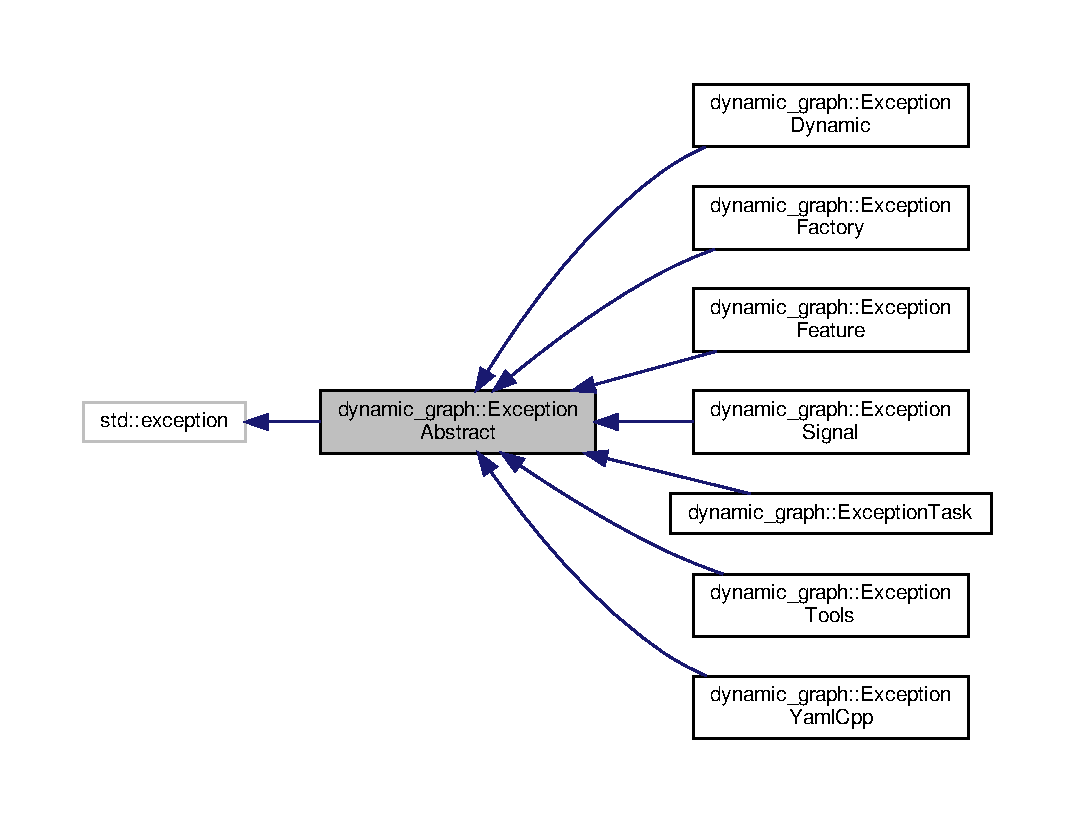
\includegraphics[width=350pt]{classdynamic__graph_1_1ExceptionAbstract__inherit__graph}
\end{center}
\end{figure}


Collaboration diagram for dynamic\+\_\+graph\+:\+:Exception\+Abstract\+:
\nopagebreak
\begin{figure}[H]
\begin{center}
\leavevmode
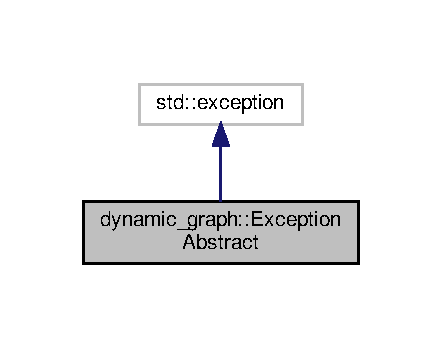
\includegraphics[width=212pt]{classdynamic__graph_1_1ExceptionAbstract__coll__graph}
\end{center}
\end{figure}
\subsection*{Public Types}
\begin{DoxyCompactItemize}
\item 
enum {\bfseries Exception\+Enum} \{ \\*
{\bfseries A\+B\+S\+T\+R\+A\+CT} = 0, 
{\bfseries S\+I\+G\+N\+AL} = 100, 
{\bfseries T\+A\+SK} = 200, 
{\bfseries F\+E\+A\+T\+U\+RE} = 300, 
\\*
{\bfseries F\+A\+C\+T\+O\+RY} = 400, 
{\bfseries D\+Y\+N\+A\+M\+IC} = 500, 
{\bfseries T\+R\+A\+C\+ES} = 600, 
{\bfseries T\+O\+O\+LS} = 700, 
\\*
{\bfseries P\+A\+T\+T\+E\+R\+N\+\_\+\+G\+E\+N\+E\+R\+A\+T\+OR} = 800, 
{\bfseries Y\+A\+M\+L\+\_\+\+C\+P\+P\+\_\+\+P\+A\+R\+S\+I\+NG} = 900
 \}\hypertarget{classdynamic__graph_1_1ExceptionAbstract_a6c51d9c9d422045a68340908bb766ee9}{}\label{classdynamic__graph_1_1ExceptionAbstract_a6c51d9c9d422045a68340908bb766ee9}

\end{DoxyCompactItemize}
\subsection*{Public Member Functions}
\begin{DoxyCompactItemize}
\item 
virtual const std\+::string \& {\bfseries get\+Exception\+Name} (void) const \hypertarget{classdynamic__graph_1_1ExceptionAbstract_abb73780d0cdd051bae35776de6ebc47c}{}\label{classdynamic__graph_1_1ExceptionAbstract_abb73780d0cdd051bae35776de6ebc47c}

\item 
{\bfseries Exception\+Abstract} (const int \&\hyperlink{classdynamic__graph_1_1ExceptionAbstract_a160cf3cd35aad75738f8b26c5cec6fdc}{code}, const std\+::string \&msg=\char`\"{}\char`\"{})\hypertarget{classdynamic__graph_1_1ExceptionAbstract_a92d849e378aca22a59aa5294ed9717bb}{}\label{classdynamic__graph_1_1ExceptionAbstract_a92d849e378aca22a59aa5294ed9717bb}

\item 
int \hyperlink{classdynamic__graph_1_1ExceptionAbstract_a4b3009fb1517a2e382026c31ef618526}{get\+Code} (void)
\begin{DoxyCompactList}\small\item\em Access to the error code. \end{DoxyCompactList}\item 
const std\+::string \& \hyperlink{classdynamic__graph_1_1ExceptionAbstract_ab43a64baae9d779737b03c7c1fbb6919}{get\+String\+Message} (void)
\begin{DoxyCompactList}\small\item\em Reference access to the error message (can be empty). \end{DoxyCompactList}\item 
const char $\ast$ \hyperlink{classdynamic__graph_1_1ExceptionAbstract_aa7b63b9c5529a7d07d5a9a880bf9a0a5}{get\+Message} (void)
\begin{DoxyCompactList}\small\item\em Access to the pointer on the array of {\itshape char} related to the error string. \end{DoxyCompactList}\item 
const char $\ast$ {\bfseries what} () const   throw ()\hypertarget{classdynamic__graph_1_1ExceptionAbstract_af9fd492effc5a20e9c7a50bfb1f04e61}{}\label{classdynamic__graph_1_1ExceptionAbstract_af9fd492effc5a20e9c7a50bfb1f04e61}

\end{DoxyCompactItemize}
\subsection*{Static Public Attributes}
\begin{DoxyCompactItemize}
\item 
static const std\+::string {\bfseries E\+X\+C\+E\+P\+T\+I\+O\+N\+\_\+\+N\+A\+ME} = \char`\"{}Abstract\char`\"{}\hypertarget{classdynamic__graph_1_1ExceptionAbstract_a3fe66d505c81575f26360298171c9e50}{}\label{classdynamic__graph_1_1ExceptionAbstract_a3fe66d505c81575f26360298171c9e50}

\end{DoxyCompactItemize}
\subsection*{Protected Attributes}
\begin{DoxyCompactItemize}
\item 
int \hyperlink{classdynamic__graph_1_1ExceptionAbstract_a160cf3cd35aad75738f8b26c5cec6fdc}{code}
\begin{DoxyCompactList}\small\item\em Error code. \end{DoxyCompactList}\item 
std\+::string \hyperlink{classdynamic__graph_1_1ExceptionAbstract_a9622b93d152c08ab80ed4b48ea24380b}{message}
\begin{DoxyCompactList}\small\item\em Error message (can be empty). \end{DoxyCompactList}\end{DoxyCompactItemize}
\subsection*{Private Member Functions}
\begin{DoxyCompactItemize}
\item 
\hyperlink{classdynamic__graph_1_1ExceptionAbstract_a474009850ce7a50c121e4c4294181e79}{Exception\+Abstract} (void)
\begin{DoxyCompactList}\small\item\em forbid the empty constructor (private). \end{DoxyCompactList}\end{DoxyCompactItemize}
\subsection*{Friends}
\begin{DoxyCompactItemize}
\item 
std\+::ostream \& \hyperlink{classdynamic__graph_1_1ExceptionAbstract_af1ab4fed15cda5c7de2c9c4f809bd611}{operator$<$$<$} (std\+::ostream \&os, const \hyperlink{classdynamic__graph_1_1ExceptionAbstract}{Exception\+Abstract} \&err)
\begin{DoxyCompactList}\small\item\em Print the error structure. \end{DoxyCompactList}\end{DoxyCompactItemize}


\subsection{Detailed Description}
The \hyperlink{classdynamic__graph_1_1ExceptionAbstract}{Exception\+Abstract} class. 

\subsection{Constructor \& Destructor Documentation}
\index{dynamic\+\_\+graph\+::\+Exception\+Abstract@{dynamic\+\_\+graph\+::\+Exception\+Abstract}!Exception\+Abstract@{Exception\+Abstract}}
\index{Exception\+Abstract@{Exception\+Abstract}!dynamic\+\_\+graph\+::\+Exception\+Abstract@{dynamic\+\_\+graph\+::\+Exception\+Abstract}}
\subsubsection[{\texorpdfstring{Exception\+Abstract(void)}{ExceptionAbstract(void)}}]{\setlength{\rightskip}{0pt plus 5cm}dynamic\+\_\+graph\+::\+Exception\+Abstract\+::\+Exception\+Abstract (
\begin{DoxyParamCaption}
\item[{void}]{}
\end{DoxyParamCaption}
)\hspace{0.3cm}{\ttfamily [private]}}\hypertarget{classdynamic__graph_1_1ExceptionAbstract_a474009850ce7a50c121e4c4294181e79}{}\label{classdynamic__graph_1_1ExceptionAbstract_a474009850ce7a50c121e4c4294181e79}


forbid the empty constructor (private). 



\subsection{Member Function Documentation}
\index{dynamic\+\_\+graph\+::\+Exception\+Abstract@{dynamic\+\_\+graph\+::\+Exception\+Abstract}!get\+Code@{get\+Code}}
\index{get\+Code@{get\+Code}!dynamic\+\_\+graph\+::\+Exception\+Abstract@{dynamic\+\_\+graph\+::\+Exception\+Abstract}}
\subsubsection[{\texorpdfstring{get\+Code(void)}{getCode(void)}}]{\setlength{\rightskip}{0pt plus 5cm}int Exception\+Abstract\+::get\+Code (
\begin{DoxyParamCaption}
\item[{void}]{}
\end{DoxyParamCaption}
)}\hypertarget{classdynamic__graph_1_1ExceptionAbstract_a4b3009fb1517a2e382026c31ef618526}{}\label{classdynamic__graph_1_1ExceptionAbstract_a4b3009fb1517a2e382026c31ef618526}


Access to the error code. 

\index{dynamic\+\_\+graph\+::\+Exception\+Abstract@{dynamic\+\_\+graph\+::\+Exception\+Abstract}!get\+Message@{get\+Message}}
\index{get\+Message@{get\+Message}!dynamic\+\_\+graph\+::\+Exception\+Abstract@{dynamic\+\_\+graph\+::\+Exception\+Abstract}}
\subsubsection[{\texorpdfstring{get\+Message(void)}{getMessage(void)}}]{\setlength{\rightskip}{0pt plus 5cm}const char $\ast$ Exception\+Abstract\+::get\+Message (
\begin{DoxyParamCaption}
\item[{void}]{}
\end{DoxyParamCaption}
)}\hypertarget{classdynamic__graph_1_1ExceptionAbstract_aa7b63b9c5529a7d07d5a9a880bf9a0a5}{}\label{classdynamic__graph_1_1ExceptionAbstract_aa7b63b9c5529a7d07d5a9a880bf9a0a5}


Access to the pointer on the array of {\itshape char} related to the error string. 

Cannot be {\itshape N\+U\+LL}. \index{dynamic\+\_\+graph\+::\+Exception\+Abstract@{dynamic\+\_\+graph\+::\+Exception\+Abstract}!get\+String\+Message@{get\+String\+Message}}
\index{get\+String\+Message@{get\+String\+Message}!dynamic\+\_\+graph\+::\+Exception\+Abstract@{dynamic\+\_\+graph\+::\+Exception\+Abstract}}
\subsubsection[{\texorpdfstring{get\+String\+Message(void)}{getStringMessage(void)}}]{\setlength{\rightskip}{0pt plus 5cm}const string \& Exception\+Abstract\+::get\+String\+Message (
\begin{DoxyParamCaption}
\item[{void}]{}
\end{DoxyParamCaption}
)}\hypertarget{classdynamic__graph_1_1ExceptionAbstract_ab43a64baae9d779737b03c7c1fbb6919}{}\label{classdynamic__graph_1_1ExceptionAbstract_ab43a64baae9d779737b03c7c1fbb6919}


Reference access to the error message (can be empty). 



\subsection{Friends And Related Function Documentation}
\index{dynamic\+\_\+graph\+::\+Exception\+Abstract@{dynamic\+\_\+graph\+::\+Exception\+Abstract}!operator$<$$<$@{operator$<$$<$}}
\index{operator$<$$<$@{operator$<$$<$}!dynamic\+\_\+graph\+::\+Exception\+Abstract@{dynamic\+\_\+graph\+::\+Exception\+Abstract}}
\subsubsection[{\texorpdfstring{operator$<$$<$}{operator<<}}]{\setlength{\rightskip}{0pt plus 5cm}std\+::ostream\& operator$<$$<$ (
\begin{DoxyParamCaption}
\item[{std\+::ostream \&}]{os, }
\item[{const {\bf Exception\+Abstract} \&}]{err}
\end{DoxyParamCaption}
)\hspace{0.3cm}{\ttfamily [friend]}}\hypertarget{classdynamic__graph_1_1ExceptionAbstract_af1ab4fed15cda5c7de2c9c4f809bd611}{}\label{classdynamic__graph_1_1ExceptionAbstract_af1ab4fed15cda5c7de2c9c4f809bd611}


Print the error structure. 



\subsection{Member Data Documentation}
\index{dynamic\+\_\+graph\+::\+Exception\+Abstract@{dynamic\+\_\+graph\+::\+Exception\+Abstract}!code@{code}}
\index{code@{code}!dynamic\+\_\+graph\+::\+Exception\+Abstract@{dynamic\+\_\+graph\+::\+Exception\+Abstract}}
\subsubsection[{\texorpdfstring{code}{code}}]{\setlength{\rightskip}{0pt plus 5cm}int dynamic\+\_\+graph\+::\+Exception\+Abstract\+::code\hspace{0.3cm}{\ttfamily [protected]}}\hypertarget{classdynamic__graph_1_1ExceptionAbstract_a160cf3cd35aad75738f8b26c5cec6fdc}{}\label{classdynamic__graph_1_1ExceptionAbstract_a160cf3cd35aad75738f8b26c5cec6fdc}


Error code. 

\begin{DoxySeeAlso}{See also}
Error\+Code\+Enum 
\end{DoxySeeAlso}
\index{dynamic\+\_\+graph\+::\+Exception\+Abstract@{dynamic\+\_\+graph\+::\+Exception\+Abstract}!message@{message}}
\index{message@{message}!dynamic\+\_\+graph\+::\+Exception\+Abstract@{dynamic\+\_\+graph\+::\+Exception\+Abstract}}
\subsubsection[{\texorpdfstring{message}{message}}]{\setlength{\rightskip}{0pt plus 5cm}std\+::string dynamic\+\_\+graph\+::\+Exception\+Abstract\+::message\hspace{0.3cm}{\ttfamily [protected]}}\hypertarget{classdynamic__graph_1_1ExceptionAbstract_a9622b93d152c08ab80ed4b48ea24380b}{}\label{classdynamic__graph_1_1ExceptionAbstract_a9622b93d152c08ab80ed4b48ea24380b}


Error message (can be empty). 



The documentation for this class was generated from the following files\+:\begin{DoxyCompactItemize}
\item 
include/dynamic\+\_\+graph\+\_\+manager/exception/\hyperlink{exception-abstract_8hh}{exception-\/abstract.\+hh}\item 
src/exception/\hyperlink{exception-abstract_8cpp}{exception-\/abstract.\+cpp}\end{DoxyCompactItemize}

\hypertarget{classdynamic__graph_1_1ExceptionDynamic}{}\section{dynamic\+\_\+graph\+:\+:Exception\+Dynamic Class Reference}
\label{classdynamic__graph_1_1ExceptionDynamic}\index{dynamic\+\_\+graph\+::\+Exception\+Dynamic@{dynamic\+\_\+graph\+::\+Exception\+Dynamic}}


\hyperlink{classdynamic__graph_1_1ExceptionDynamic}{Exception\+Dynamic}.  




{\ttfamily \#include $<$exception-\/dynamic.\+hh$>$}



Inheritance diagram for dynamic\+\_\+graph\+:\+:Exception\+Dynamic\+:
\nopagebreak
\begin{figure}[H]
\begin{center}
\leavevmode
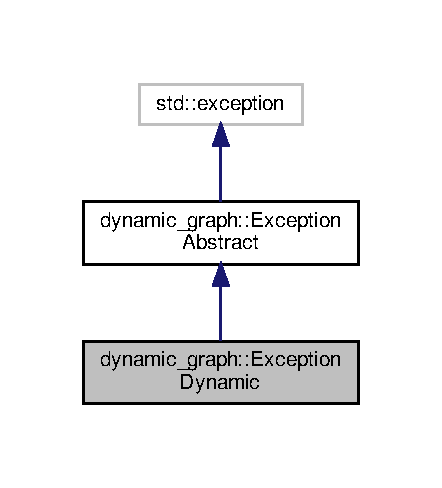
\includegraphics[width=212pt]{classdynamic__graph_1_1ExceptionDynamic__inherit__graph}
\end{center}
\end{figure}


Collaboration diagram for dynamic\+\_\+graph\+:\+:Exception\+Dynamic\+:
\nopagebreak
\begin{figure}[H]
\begin{center}
\leavevmode
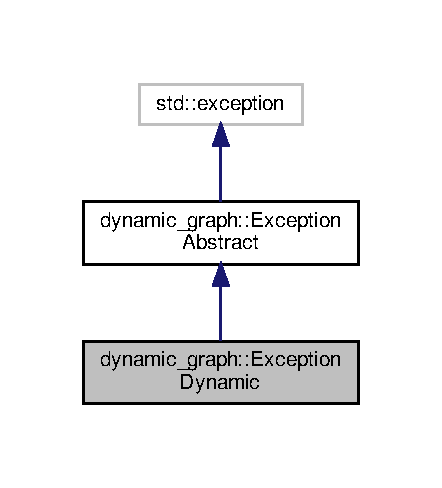
\includegraphics[width=212pt]{classdynamic__graph_1_1ExceptionDynamic__coll__graph}
\end{center}
\end{figure}
\subsection*{Public Types}
\begin{DoxyCompactItemize}
\item 
enum {\bfseries Error\+Code\+Enum} \{ \\*
{\bfseries G\+E\+N\+E\+R\+IC} = Exception\+Abstract\+:\+:D\+Y\+N\+A\+M\+IC, 
{\bfseries C\+A\+N\+T\+\_\+\+D\+E\+S\+T\+R\+O\+Y\+\_\+\+S\+I\+G\+N\+AL}, 
{\bfseries J\+O\+I\+N\+T\+\_\+\+R\+A\+NK}, 
{\bfseries D\+Y\+N\+A\+M\+I\+C\+\_\+\+J\+RL}, 
\\*
{\bfseries J\+O\+I\+N\+T\+\_\+\+S\+I\+ZE}, 
{\bfseries I\+N\+T\+E\+G\+R\+A\+T\+I\+ON}
 \}\hypertarget{classdynamic__graph_1_1ExceptionDynamic_a928d14f0f9bbd488f42a2d7577fb341b}{}\label{classdynamic__graph_1_1ExceptionDynamic_a928d14f0f9bbd488f42a2d7577fb341b}

\end{DoxyCompactItemize}
\subsection*{Public Member Functions}
\begin{DoxyCompactItemize}
\item 
virtual const std\+::string \& {\bfseries get\+Exception\+Name} (void) const \hypertarget{classdynamic__graph_1_1ExceptionDynamic_ab70632639ed4d4b00d9d3840c710d414}{}\label{classdynamic__graph_1_1ExceptionDynamic_ab70632639ed4d4b00d9d3840c710d414}

\item 
{\bfseries Exception\+Dynamic} (const Exception\+Dynamic\+::\+Error\+Code\+Enum \&errcode, const std\+::string \&msg=\char`\"{}\char`\"{})\hypertarget{classdynamic__graph_1_1ExceptionDynamic_a733c68c022311f9418a97fe1687c813a}{}\label{classdynamic__graph_1_1ExceptionDynamic_a733c68c022311f9418a97fe1687c813a}

\item 
{\bfseries Exception\+Dynamic} (const Exception\+Dynamic\+::\+Error\+Code\+Enum \&errcode, const std\+::string \&msg, const char $\ast$format,...)\hypertarget{classdynamic__graph_1_1ExceptionDynamic_a5f5cdec1772f2cbd833b0134bfcb0980}{}\label{classdynamic__graph_1_1ExceptionDynamic_a5f5cdec1772f2cbd833b0134bfcb0980}

\end{DoxyCompactItemize}
\subsection*{Static Public Attributes}
\begin{DoxyCompactItemize}
\item 
static const std\+::string {\bfseries E\+X\+C\+E\+P\+T\+I\+O\+N\+\_\+\+N\+A\+ME} = \char`\"{}Dynamic\char`\"{}\hypertarget{classdynamic__graph_1_1ExceptionDynamic_a29aa1b98aa4219a3a99ae314f2b8c1ef}{}\label{classdynamic__graph_1_1ExceptionDynamic_a29aa1b98aa4219a3a99ae314f2b8c1ef}

\end{DoxyCompactItemize}
\subsection*{Additional Inherited Members}


\subsection{Detailed Description}
\hyperlink{classdynamic__graph_1_1ExceptionDynamic}{Exception\+Dynamic}. 

The documentation for this class was generated from the following files\+:\begin{DoxyCompactItemize}
\item 
include/dynamic\+\_\+graph\+\_\+manager/exception/\hyperlink{exception-dynamic_8hh}{exception-\/dynamic.\+hh}\item 
src/exception/\hyperlink{exception-dynamic_8cpp}{exception-\/dynamic.\+cpp}\end{DoxyCompactItemize}

\hypertarget{classdynamic__graph_1_1ExceptionFactory}{}\section{dynamic\+\_\+graph\+:\+:Exception\+Factory Class Reference}
\label{classdynamic__graph_1_1ExceptionFactory}\index{dynamic\+\_\+graph\+::\+Exception\+Factory@{dynamic\+\_\+graph\+::\+Exception\+Factory}}


The \hyperlink{classdynamic__graph_1_1ExceptionFactory}{Exception\+Factory} class.  




{\ttfamily \#include $<$exception-\/factory.\+hh$>$}



Inheritance diagram for dynamic\+\_\+graph\+:\+:Exception\+Factory\+:\nopagebreak
\begin{figure}[H]
\begin{center}
\leavevmode
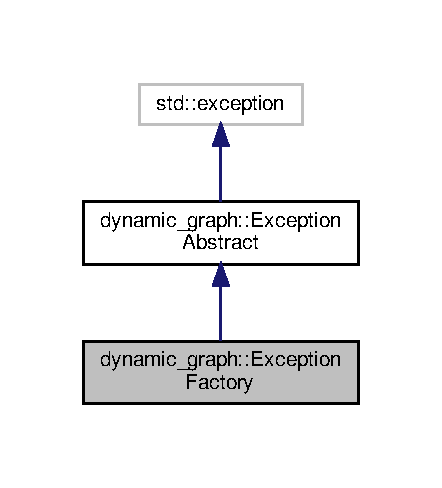
\includegraphics[width=212pt]{classdynamic__graph_1_1ExceptionFactory__inherit__graph}
\end{center}
\end{figure}


Collaboration diagram for dynamic\+\_\+graph\+:\+:Exception\+Factory\+:\nopagebreak
\begin{figure}[H]
\begin{center}
\leavevmode
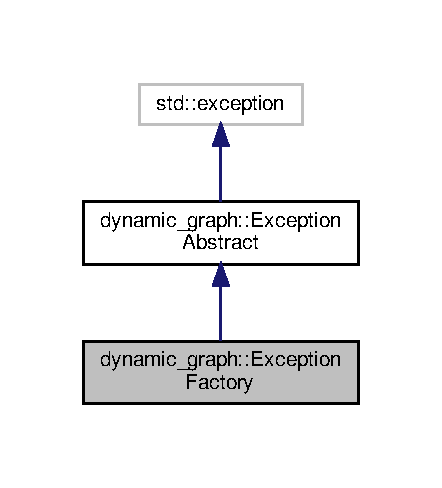
\includegraphics[width=212pt]{classdynamic__graph_1_1ExceptionFactory__coll__graph}
\end{center}
\end{figure}
\subsection*{Public Types}
\begin{DoxyCompactItemize}
\item 
enum {\bfseries Error\+Code\+Enum} \{ \\*
{\bfseries G\+E\+N\+E\+R\+IC} = Exception\+Abstract\+:\+:F\+A\+C\+T\+O\+RY, 
{\bfseries U\+N\+R\+E\+F\+E\+R\+E\+D\+\_\+\+O\+B\+J\+E\+CT}, 
{\bfseries U\+N\+R\+E\+F\+E\+R\+E\+D\+\_\+\+S\+I\+G\+N\+AL}, 
{\bfseries U\+N\+R\+E\+F\+E\+R\+E\+D\+\_\+\+F\+U\+N\+C\+T\+I\+ON}, 
\\*
{\bfseries D\+Y\+N\+A\+M\+I\+C\+\_\+\+L\+O\+A\+D\+I\+NG}, 
{\bfseries S\+I\+G\+N\+A\+L\+\_\+\+C\+O\+N\+F\+L\+I\+CT}, 
{\bfseries F\+U\+N\+C\+T\+I\+O\+N\+\_\+\+C\+O\+N\+F\+L\+I\+CT}, 
{\bfseries O\+B\+J\+E\+C\+T\+\_\+\+C\+O\+N\+F\+L\+I\+CT}, 
\\*
{\bfseries S\+Y\+N\+T\+A\+X\+\_\+\+E\+R\+R\+OR}, 
{\bfseries R\+E\+A\+D\+\_\+\+F\+I\+LE}
 \}\hypertarget{classdynamic__graph_1_1ExceptionFactory_a61ed67b84bf03809ef3d6b4124e4c39d}{}\label{classdynamic__graph_1_1ExceptionFactory_a61ed67b84bf03809ef3d6b4124e4c39d}

\end{DoxyCompactItemize}
\subsection*{Public Member Functions}
\begin{DoxyCompactItemize}
\item 
virtual const std\+::string \& {\bfseries get\+Exception\+Name} (void) const \hypertarget{classdynamic__graph_1_1ExceptionFactory_ad7b2f2a7bf8dc47d3e5221e6c0b3a8ab}{}\label{classdynamic__graph_1_1ExceptionFactory_ad7b2f2a7bf8dc47d3e5221e6c0b3a8ab}

\item 
{\bfseries Exception\+Factory} (const Exception\+Factory\+::\+Error\+Code\+Enum \&errcode, const std\+::string \&msg=\char`\"{}\char`\"{})\hypertarget{classdynamic__graph_1_1ExceptionFactory_a761ecdb7e256d8e08ef57d8a30aa0304}{}\label{classdynamic__graph_1_1ExceptionFactory_a761ecdb7e256d8e08ef57d8a30aa0304}

\item 
{\bfseries Exception\+Factory} (const Exception\+Factory\+::\+Error\+Code\+Enum \&errcode, const std\+::string \&msg, const char $\ast$format,...)\hypertarget{classdynamic__graph_1_1ExceptionFactory_a7cf2af98062079786409dc9a2dcfd85a}{}\label{classdynamic__graph_1_1ExceptionFactory_a7cf2af98062079786409dc9a2dcfd85a}

\end{DoxyCompactItemize}
\subsection*{Static Public Attributes}
\begin{DoxyCompactItemize}
\item 
static const std\+::string {\bfseries E\+X\+C\+E\+P\+T\+I\+O\+N\+\_\+\+N\+A\+ME} = \char`\"{}Factory\char`\"{}\hypertarget{classdynamic__graph_1_1ExceptionFactory_a7fe66d9197d860bd55f3a9676fa489b1}{}\label{classdynamic__graph_1_1ExceptionFactory_a7fe66d9197d860bd55f3a9676fa489b1}

\end{DoxyCompactItemize}
\subsection*{Additional Inherited Members}


\subsection{Detailed Description}
The \hyperlink{classdynamic__graph_1_1ExceptionFactory}{Exception\+Factory} class. 

The documentation for this class was generated from the following files\+:\begin{DoxyCompactItemize}
\item 
/home/mnaveau/devel/workspace/src/catkin/dg\+\_\+control/dynamic\+\_\+graph\+\_\+manager/include/dynamic\+\_\+graph\+\_\+manager/exception/\hyperlink{exception-factory_8hh}{exception-\/factory.\+hh}\item 
/home/mnaveau/devel/workspace/src/catkin/dg\+\_\+control/dynamic\+\_\+graph\+\_\+manager/src/exception/\hyperlink{exception-factory_8cpp}{exception-\/factory.\+cpp}\end{DoxyCompactItemize}

\hypertarget{classdynamic__graph_1_1ExceptionFeature}{}\section{dynamic\+\_\+graph\+:\+:Exception\+Feature Class Reference}
\label{classdynamic__graph_1_1ExceptionFeature}\index{dynamic\+\_\+graph\+::\+Exception\+Feature@{dynamic\+\_\+graph\+::\+Exception\+Feature}}


Inheritance diagram for dynamic\+\_\+graph\+:\+:Exception\+Feature\+:
\nopagebreak
\begin{figure}[H]
\begin{center}
\leavevmode
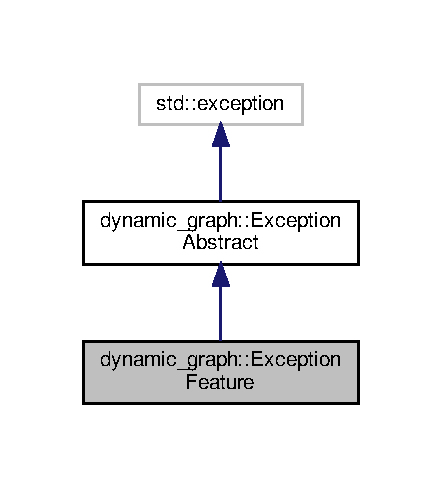
\includegraphics[width=212pt]{classdynamic__graph_1_1ExceptionFeature__inherit__graph}
\end{center}
\end{figure}


Collaboration diagram for dynamic\+\_\+graph\+:\+:Exception\+Feature\+:
\nopagebreak
\begin{figure}[H]
\begin{center}
\leavevmode
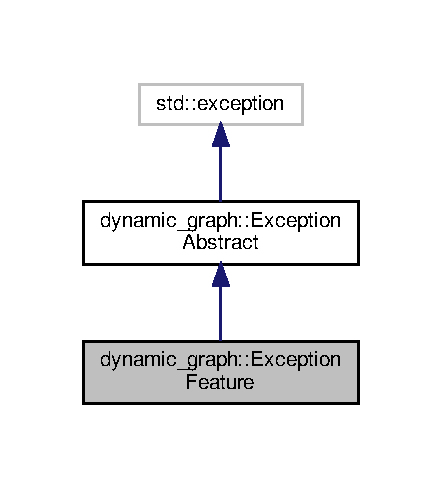
\includegraphics[width=212pt]{classdynamic__graph_1_1ExceptionFeature__coll__graph}
\end{center}
\end{figure}
\subsection*{Public Types}
\begin{DoxyCompactItemize}
\item 
\mbox{\Hypertarget{classdynamic__graph_1_1ExceptionFeature_a0699b7c4631350c8c1c0eb39a11426f1}\label{classdynamic__graph_1_1ExceptionFeature_a0699b7c4631350c8c1c0eb39a11426f1}} 
enum {\bfseries Error\+Code\+Enum} \{ {\bfseries G\+E\+N\+E\+R\+IC} = Exception\+Abstract\+:\+:F\+E\+A\+T\+U\+RE, 
{\bfseries B\+A\+D\+\_\+\+I\+N\+IT}, 
{\bfseries U\+N\+C\+O\+M\+P\+A\+T\+I\+B\+L\+E\+\_\+\+S\+I\+ZE}
 \}
\end{DoxyCompactItemize}
\subsection*{Public Member Functions}
\begin{DoxyCompactItemize}
\item 
\mbox{\Hypertarget{classdynamic__graph_1_1ExceptionFeature_a22989c5bbe6eefecef6988cd56dab002}\label{classdynamic__graph_1_1ExceptionFeature_a22989c5bbe6eefecef6988cd56dab002}} 
virtual const std\+::string \& {\bfseries get\+Exception\+Name} (void) const
\item 
\mbox{\Hypertarget{classdynamic__graph_1_1ExceptionFeature_a76a3b0adc5f5881b8b3609ddf989f24a}\label{classdynamic__graph_1_1ExceptionFeature_a76a3b0adc5f5881b8b3609ddf989f24a}} 
{\bfseries Exception\+Feature} (const Exception\+Feature\+::\+Error\+Code\+Enum \&errcode, const std\+::string \&msg=\char`\"{}\char`\"{})
\item 
\mbox{\Hypertarget{classdynamic__graph_1_1ExceptionFeature_a88a704700091fa451ee9bc6db1ad793e}\label{classdynamic__graph_1_1ExceptionFeature_a88a704700091fa451ee9bc6db1ad793e}} 
{\bfseries Exception\+Feature} (const Exception\+Feature\+::\+Error\+Code\+Enum \&errcode, const std\+::string \&msg, const char $\ast$format,...)
\end{DoxyCompactItemize}
\subsection*{Static Public Attributes}
\begin{DoxyCompactItemize}
\item 
\mbox{\Hypertarget{classdynamic__graph_1_1ExceptionFeature_a977865e1bf4940aed64bf434ec72bf18}\label{classdynamic__graph_1_1ExceptionFeature_a977865e1bf4940aed64bf434ec72bf18}} 
static const std\+::string {\bfseries E\+X\+C\+E\+P\+T\+I\+O\+N\+\_\+\+N\+A\+ME} = \char`\"{}Feature\char`\"{}
\end{DoxyCompactItemize}
\subsection*{Additional Inherited Members}


The documentation for this class was generated from the following files\+:\begin{DoxyCompactItemize}
\item 
include/dynamic\+\_\+graph\+\_\+manager/exception/\hyperlink{exception-feature_8hh}{exception-\/feature.\+hh}\item 
src/exception/\hyperlink{exception-feature_8cpp}{exception-\/feature.\+cpp}\end{DoxyCompactItemize}

\hypertarget{classdynamic__graph_1_1ExceptionSignal}{}\section{dynamic\+\_\+graph\+:\+:Exception\+Signal Class Reference}
\label{classdynamic__graph_1_1ExceptionSignal}\index{dynamic\+\_\+graph\+::\+Exception\+Signal@{dynamic\+\_\+graph\+::\+Exception\+Signal}}


Inheritance diagram for dynamic\+\_\+graph\+:\+:Exception\+Signal\+:\nopagebreak
\begin{figure}[H]
\begin{center}
\leavevmode
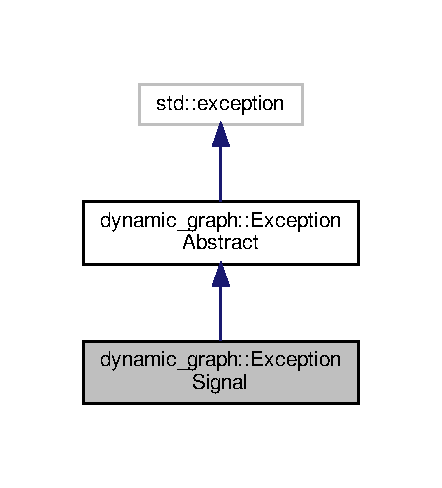
\includegraphics[width=212pt]{classdynamic__graph_1_1ExceptionSignal__inherit__graph}
\end{center}
\end{figure}


Collaboration diagram for dynamic\+\_\+graph\+:\+:Exception\+Signal\+:\nopagebreak
\begin{figure}[H]
\begin{center}
\leavevmode
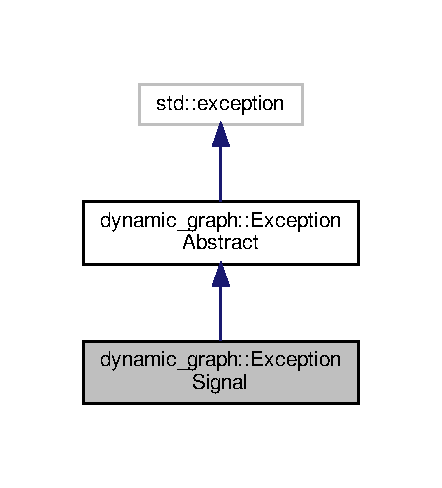
\includegraphics[width=212pt]{classdynamic__graph_1_1ExceptionSignal__coll__graph}
\end{center}
\end{figure}
\subsection*{Public Types}
\begin{DoxyCompactItemize}
\item 
enum {\bfseries Error\+Code\+Enum} \{ \\*
{\bfseries G\+E\+N\+E\+R\+IC} = Exception\+Abstract\+:\+:S\+I\+G\+N\+AL, 
{\bfseries R\+E\+A\+D\+W\+R\+I\+T\+E\+\_\+\+L\+O\+CK}, 
{\bfseries C\+O\+P\+Y\+\_\+\+N\+O\+T\+\_\+\+I\+N\+I\+T\+I\+A\+L\+I\+Z\+ED}, 
{\bfseries N\+O\+T\+\_\+\+I\+N\+I\+T\+I\+A\+L\+I\+Z\+ED}, 
\\*
{\bfseries P\+L\+U\+G\+\_\+\+I\+M\+P\+O\+S\+S\+I\+B\+LE}, 
{\bfseries S\+E\+T\+\_\+\+I\+M\+P\+O\+S\+S\+I\+B\+LE}, 
{\bfseries B\+A\+D\+\_\+\+C\+A\+ST}
 \}\hypertarget{classdynamic__graph_1_1ExceptionSignal_a122fbe147d0fd92c511f5839394e2bc1}{}\label{classdynamic__graph_1_1ExceptionSignal_a122fbe147d0fd92c511f5839394e2bc1}

\end{DoxyCompactItemize}
\subsection*{Public Member Functions}
\begin{DoxyCompactItemize}
\item 
virtual const std\+::string \& {\bfseries get\+Exception\+Name} (void) const \hypertarget{classdynamic__graph_1_1ExceptionSignal_ad9503d0b270c9a992f8f7798ef4d62d1}{}\label{classdynamic__graph_1_1ExceptionSignal_ad9503d0b270c9a992f8f7798ef4d62d1}

\item 
{\bfseries Exception\+Signal} (const Exception\+Signal\+::\+Error\+Code\+Enum \&errcode, const std\+::string \&msg=\char`\"{}\char`\"{})\hypertarget{classdynamic__graph_1_1ExceptionSignal_aad0d2b0f022ca8bfc8ce3a9e81475d52}{}\label{classdynamic__graph_1_1ExceptionSignal_aad0d2b0f022ca8bfc8ce3a9e81475d52}

\item 
{\bfseries Exception\+Signal} (const Exception\+Signal\+::\+Error\+Code\+Enum \&errcode, const std\+::string \&msg, const char $\ast$format,...)\hypertarget{classdynamic__graph_1_1ExceptionSignal_a8b317aa83e16632ce3ce6e6c833acb91}{}\label{classdynamic__graph_1_1ExceptionSignal_a8b317aa83e16632ce3ce6e6c833acb91}

\end{DoxyCompactItemize}
\subsection*{Static Public Attributes}
\begin{DoxyCompactItemize}
\item 
static const std\+::string {\bfseries E\+X\+C\+E\+P\+T\+I\+O\+N\+\_\+\+N\+A\+ME} = \char`\"{}Signal\char`\"{}\hypertarget{classdynamic__graph_1_1ExceptionSignal_a3f08eaf0b6f59dffaa47e844387e978b}{}\label{classdynamic__graph_1_1ExceptionSignal_a3f08eaf0b6f59dffaa47e844387e978b}

\end{DoxyCompactItemize}
\subsection*{Additional Inherited Members}


The documentation for this class was generated from the following files\+:\begin{DoxyCompactItemize}
\item 
/home/mnaveau/devel/workspace/src/catkin/dg\+\_\+control/dynamic\+\_\+graph\+\_\+manager/include/dynamic\+\_\+graph\+\_\+manager/exception/\hyperlink{exception-signal_8hh}{exception-\/signal.\+hh}\item 
/home/mnaveau/devel/workspace/src/catkin/dg\+\_\+control/dynamic\+\_\+graph\+\_\+manager/src/exception/\hyperlink{exception-signal_8cpp}{exception-\/signal.\+cpp}\end{DoxyCompactItemize}

\hypertarget{classdynamic__graph_1_1ExceptionTask}{}\section{dynamic\+\_\+graph\+:\+:Exception\+Task Class Reference}
\label{classdynamic__graph_1_1ExceptionTask}\index{dynamic\+\_\+graph\+::\+Exception\+Task@{dynamic\+\_\+graph\+::\+Exception\+Task}}


\hyperlink{classdynamic__graph_1_1ExceptionTask}{Exception\+Task}.  




{\ttfamily \#include $<$exception-\/task.\+hh$>$}



Inheritance diagram for dynamic\+\_\+graph\+:\+:Exception\+Task\+:
\nopagebreak
\begin{figure}[H]
\begin{center}
\leavevmode
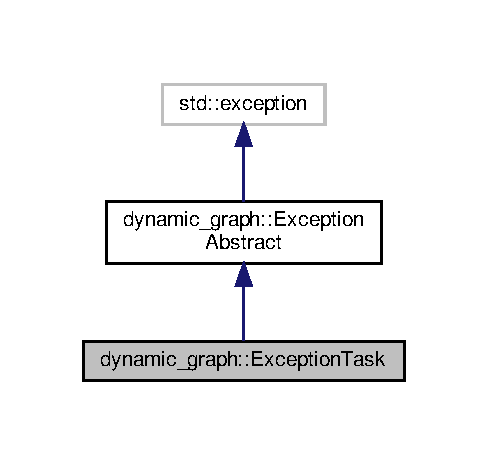
\includegraphics[width=234pt]{classdynamic__graph_1_1ExceptionTask__inherit__graph}
\end{center}
\end{figure}


Collaboration diagram for dynamic\+\_\+graph\+:\+:Exception\+Task\+:
\nopagebreak
\begin{figure}[H]
\begin{center}
\leavevmode
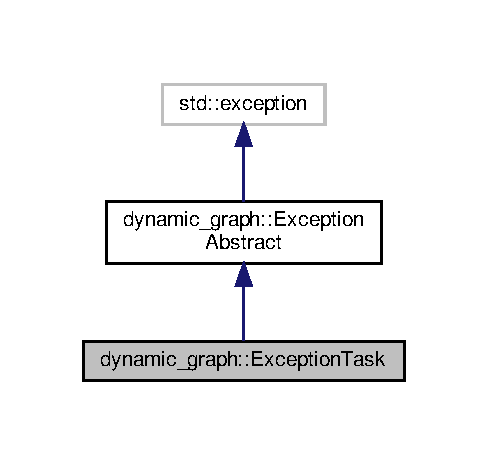
\includegraphics[width=234pt]{classdynamic__graph_1_1ExceptionTask__coll__graph}
\end{center}
\end{figure}
\subsection*{Public Types}
\begin{DoxyCompactItemize}
\item 
enum {\bfseries Error\+Code\+Enum} \{ \\*
{\bfseries G\+E\+N\+E\+R\+IC} = Exception\+Abstract\+:\+:T\+A\+SK, 
{\bfseries E\+M\+P\+T\+Y\+\_\+\+L\+I\+ST}, 
{\bfseries N\+O\+N\+\_\+\+A\+D\+E\+Q\+U\+A\+T\+E\+\_\+\+F\+E\+A\+T\+U\+R\+ES}, 
{\bfseries M\+A\+T\+R\+I\+X\+\_\+\+S\+I\+ZE}, 
\\*
{\bfseries B\+O\+U\+N\+D\+\_\+\+T\+Y\+PE}, 
{\bfseries P\+A\+R\+S\+E\+R\+\_\+\+M\+U\+L\+T\+I\+\_\+\+B\+O\+U\+ND}
 \}\hypertarget{classdynamic__graph_1_1ExceptionTask_a0ccd75121639190d176ffd062e0d69d8}{}\label{classdynamic__graph_1_1ExceptionTask_a0ccd75121639190d176ffd062e0d69d8}

\end{DoxyCompactItemize}
\subsection*{Public Member Functions}
\begin{DoxyCompactItemize}
\item 
virtual const std\+::string \& {\bfseries get\+Exception\+Name} (void) const \hypertarget{classdynamic__graph_1_1ExceptionTask_a7ed756498ca26263200532a84abc5160}{}\label{classdynamic__graph_1_1ExceptionTask_a7ed756498ca26263200532a84abc5160}

\item 
{\bfseries Exception\+Task} (const Exception\+Task\+::\+Error\+Code\+Enum \&errcode, const std\+::string \&msg=\char`\"{}\char`\"{})\hypertarget{classdynamic__graph_1_1ExceptionTask_af05ac9817dc1de874190803ed92321a8}{}\label{classdynamic__graph_1_1ExceptionTask_af05ac9817dc1de874190803ed92321a8}

\item 
{\bfseries Exception\+Task} (const Exception\+Task\+::\+Error\+Code\+Enum \&errcode, const std\+::string \&msg, const char $\ast$format,...)\hypertarget{classdynamic__graph_1_1ExceptionTask_ac9bd1b490d5758bf1c7eecaeee6cebe9}{}\label{classdynamic__graph_1_1ExceptionTask_ac9bd1b490d5758bf1c7eecaeee6cebe9}

\end{DoxyCompactItemize}
\subsection*{Static Public Attributes}
\begin{DoxyCompactItemize}
\item 
static const std\+::string {\bfseries E\+X\+C\+E\+P\+T\+I\+O\+N\+\_\+\+N\+A\+ME} = \char`\"{}Task\char`\"{}\hypertarget{classdynamic__graph_1_1ExceptionTask_ad36eb4b540be350af2b24895955dcc0a}{}\label{classdynamic__graph_1_1ExceptionTask_ad36eb4b540be350af2b24895955dcc0a}

\end{DoxyCompactItemize}
\subsection*{Additional Inherited Members}


\subsection{Detailed Description}
\hyperlink{classdynamic__graph_1_1ExceptionTask}{Exception\+Task}. 

The documentation for this class was generated from the following files\+:\begin{DoxyCompactItemize}
\item 
include/dynamic\+\_\+graph\+\_\+manager/exception/\hyperlink{exception-task_8hh}{exception-\/task.\+hh}\item 
src/exception/\hyperlink{exception-task_8cpp}{exception-\/task.\+cpp}\end{DoxyCompactItemize}

\hypertarget{classdynamic__graph_1_1ExceptionTools}{}\section{dynamic\+\_\+graph\+:\+:Exception\+Tools Class Reference}
\label{classdynamic__graph_1_1ExceptionTools}\index{dynamic\+\_\+graph\+::\+Exception\+Tools@{dynamic\+\_\+graph\+::\+Exception\+Tools}}


Inheritance diagram for dynamic\+\_\+graph\+:\+:Exception\+Tools\+:
\nopagebreak
\begin{figure}[H]
\begin{center}
\leavevmode
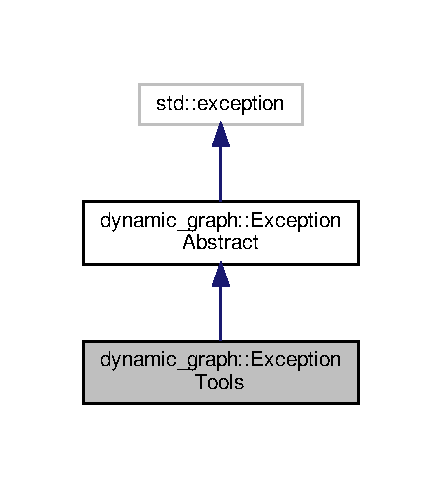
\includegraphics[width=212pt]{classdynamic__graph_1_1ExceptionTools__inherit__graph}
\end{center}
\end{figure}


Collaboration diagram for dynamic\+\_\+graph\+:\+:Exception\+Tools\+:
\nopagebreak
\begin{figure}[H]
\begin{center}
\leavevmode
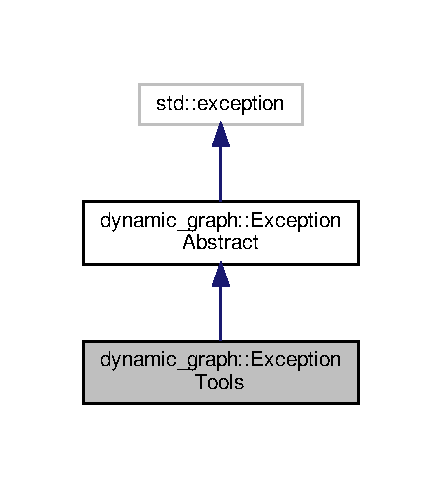
\includegraphics[width=212pt]{classdynamic__graph_1_1ExceptionTools__coll__graph}
\end{center}
\end{figure}
\subsection*{Public Types}
\begin{DoxyCompactItemize}
\item 
\mbox{\Hypertarget{classdynamic__graph_1_1ExceptionTools_a729905d84b61fe0895e80ad13982c9cb}\label{classdynamic__graph_1_1ExceptionTools_a729905d84b61fe0895e80ad13982c9cb}} 
enum {\bfseries Error\+Code\+Enum} \{ {\bfseries G\+E\+N\+E\+R\+IC} = Exception\+Abstract\+:\+:T\+O\+O\+LS, 
{\bfseries C\+O\+R\+BA}, 
{\bfseries K\+A\+L\+M\+A\+N\+\_\+\+S\+I\+ZE}, 
{\bfseries P\+Y\+\_\+\+S\+H\+E\+L\+L\+\_\+\+P\+TR}
 \}
\end{DoxyCompactItemize}
\subsection*{Public Member Functions}
\begin{DoxyCompactItemize}
\item 
\mbox{\Hypertarget{classdynamic__graph_1_1ExceptionTools_a7963a6526507f53fdb03d370cb6b3238}\label{classdynamic__graph_1_1ExceptionTools_a7963a6526507f53fdb03d370cb6b3238}} 
virtual const std\+::string \& {\bfseries get\+Exception\+Name} () const
\item 
\mbox{\Hypertarget{classdynamic__graph_1_1ExceptionTools_a215023b7c5fd241bf6493e0025172b22}\label{classdynamic__graph_1_1ExceptionTools_a215023b7c5fd241bf6493e0025172b22}} 
{\bfseries Exception\+Tools} (const Exception\+Tools\+::\+Error\+Code\+Enum \&errcode, const std\+::string \&msg=\char`\"{}\char`\"{})
\item 
\mbox{\Hypertarget{classdynamic__graph_1_1ExceptionTools_afdd3f8be1a238814b6d676ed72e7bfb6}\label{classdynamic__graph_1_1ExceptionTools_afdd3f8be1a238814b6d676ed72e7bfb6}} 
{\bfseries Exception\+Tools} (const Exception\+Tools\+::\+Error\+Code\+Enum \&errcode, const std\+::string \&msg, const char $\ast$format,...)
\end{DoxyCompactItemize}
\subsection*{Static Public Attributes}
\begin{DoxyCompactItemize}
\item 
\mbox{\Hypertarget{classdynamic__graph_1_1ExceptionTools_a80e1cf0e61c8a570e9dfc65be97efc0c}\label{classdynamic__graph_1_1ExceptionTools_a80e1cf0e61c8a570e9dfc65be97efc0c}} 
static const std\+::string {\bfseries E\+X\+C\+E\+P\+T\+I\+O\+N\+\_\+\+N\+A\+ME} = \char`\"{}Tools\char`\"{}
\end{DoxyCompactItemize}
\subsection*{Additional Inherited Members}


The documentation for this class was generated from the following files\+:\begin{DoxyCompactItemize}
\item 
include/dynamic\+\_\+graph\+\_\+manager/exception/\hyperlink{exception-tools_8hh}{exception-\/tools.\+hh}\item 
src/exception/\hyperlink{exception-tools_8cpp}{exception-\/tools.\+cpp}\end{DoxyCompactItemize}

\hypertarget{classdynamic__graph_1_1ExceptionYamlCpp}{}\section{dynamic\+\_\+graph\+:\+:Exception\+Yaml\+Cpp Class Reference}
\label{classdynamic__graph_1_1ExceptionYamlCpp}\index{dynamic\+\_\+graph\+::\+Exception\+Yaml\+Cpp@{dynamic\+\_\+graph\+::\+Exception\+Yaml\+Cpp}}


Inheritance diagram for dynamic\+\_\+graph\+:\+:Exception\+Yaml\+Cpp\+:
\nopagebreak
\begin{figure}[H]
\begin{center}
\leavevmode
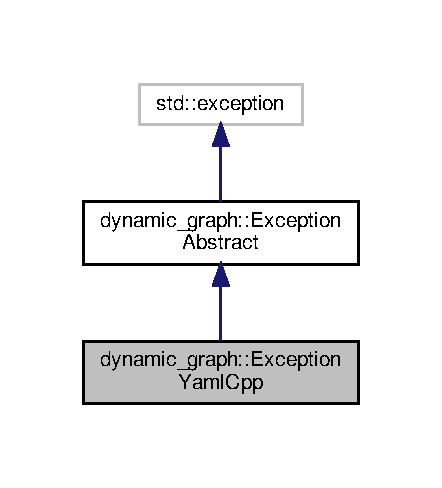
\includegraphics[width=212pt]{classdynamic__graph_1_1ExceptionYamlCpp__inherit__graph}
\end{center}
\end{figure}


Collaboration diagram for dynamic\+\_\+graph\+:\+:Exception\+Yaml\+Cpp\+:
\nopagebreak
\begin{figure}[H]
\begin{center}
\leavevmode
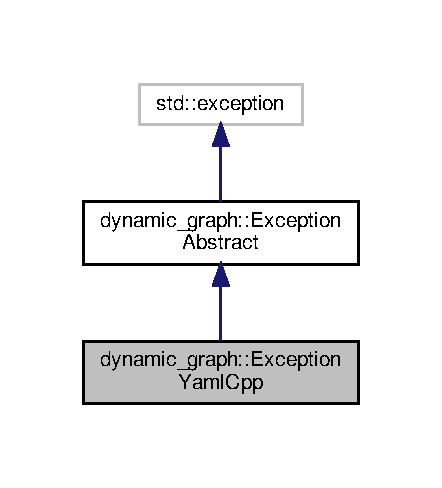
\includegraphics[width=212pt]{classdynamic__graph_1_1ExceptionYamlCpp__coll__graph}
\end{center}
\end{figure}
\subsection*{Public Types}
\begin{DoxyCompactItemize}
\item 
\mbox{\Hypertarget{classdynamic__graph_1_1ExceptionYamlCpp_aaf84f3285b4c635c35cd39aba7ac9a5a}\label{classdynamic__graph_1_1ExceptionYamlCpp_aaf84f3285b4c635c35cd39aba7ac9a5a}} 
enum {\bfseries Error\+Code\+Enum} \{ \newline
{\bfseries G\+E\+N\+E\+R\+IC} = Exception\+Abstract\+:\+:Y\+A\+M\+L\+\_\+\+C\+P\+P\+\_\+\+P\+A\+R\+S\+I\+NG, 
{\bfseries P\+A\+R\+S\+I\+N\+G\+\_\+\+B\+O\+OL}, 
{\bfseries P\+A\+R\+S\+I\+N\+G\+\_\+\+F\+L\+O\+AT}, 
{\bfseries P\+A\+R\+S\+I\+N\+G\+\_\+\+D\+O\+U\+B\+LE}, 
\newline
{\bfseries P\+A\+R\+S\+I\+N\+G\+\_\+\+E\+I\+G\+EN}, 
{\bfseries P\+A\+R\+S\+I\+N\+G\+\_\+\+S\+T\+R\+I\+NG}, 
{\bfseries P\+A\+R\+S\+I\+N\+G\+\_\+\+U\+N\+S\+I\+G\+N\+ED}
 \}
\end{DoxyCompactItemize}
\subsection*{Public Member Functions}
\begin{DoxyCompactItemize}
\item 
\mbox{\Hypertarget{classdynamic__graph_1_1ExceptionYamlCpp_aa0d7f34b8b246a8d23ce1eda5d79b80c}\label{classdynamic__graph_1_1ExceptionYamlCpp_aa0d7f34b8b246a8d23ce1eda5d79b80c}} 
virtual const std\+::string \& {\bfseries get\+Exception\+Name} () const
\item 
\mbox{\Hypertarget{classdynamic__graph_1_1ExceptionYamlCpp_ae6dc871402ab15a7af2181d3b2e5bc5e}\label{classdynamic__graph_1_1ExceptionYamlCpp_ae6dc871402ab15a7af2181d3b2e5bc5e}} 
{\bfseries Exception\+Yaml\+Cpp} (const Exception\+Yaml\+Cpp\+::\+Error\+Code\+Enum \&errcode, const std\+::string \&msg=\char`\"{}\char`\"{})
\item 
\mbox{\Hypertarget{classdynamic__graph_1_1ExceptionYamlCpp_a823359f3d24ad6930042d4d5c2443988}\label{classdynamic__graph_1_1ExceptionYamlCpp_a823359f3d24ad6930042d4d5c2443988}} 
{\bfseries Exception\+Yaml\+Cpp} (const Exception\+Yaml\+Cpp\+::\+Error\+Code\+Enum \&errcode, const std\+::string \&msg, const char $\ast$format,...)
\end{DoxyCompactItemize}
\subsection*{Static Public Attributes}
\begin{DoxyCompactItemize}
\item 
\mbox{\Hypertarget{classdynamic__graph_1_1ExceptionYamlCpp_a7d19bc2c6d36d26bd878795ea00bc63f}\label{classdynamic__graph_1_1ExceptionYamlCpp_a7d19bc2c6d36d26bd878795ea00bc63f}} 
static const std\+::string {\bfseries E\+X\+C\+E\+P\+T\+I\+O\+N\+\_\+\+N\+A\+ME} = \char`\"{}Tools\char`\"{}
\end{DoxyCompactItemize}
\subsection*{Additional Inherited Members}


The documentation for this class was generated from the following files\+:\begin{DoxyCompactItemize}
\item 
include/dynamic\+\_\+graph\+\_\+manager/exception/\hyperlink{exception-yaml-cpp_8hpp}{exception-\/yaml-\/cpp.\+hpp}\item 
src/exception/\hyperlink{exception-yaml-cpp_8cpp}{exception-\/yaml-\/cpp.\+cpp}\end{DoxyCompactItemize}

\hypertarget{structdynamic__graph_1_1GlobalRos}{}\section{dynamic\+\_\+graph\+:\+:Global\+Ros Struct Reference}
\label{structdynamic__graph_1_1GlobalRos}\index{dynamic\+\_\+graph\+::\+Global\+Ros@{dynamic\+\_\+graph\+::\+Global\+Ros}}


The \hyperlink{structdynamic__graph_1_1GlobalRos}{Global\+Ros} struct is a structure that allows to gloabally handle the R\+OS objects.  




{\ttfamily \#include $<$ros\+\_\+init.\+hh$>$}

\subsection*{Public Member Functions}
\begin{DoxyCompactItemize}
\item 
\hyperlink{structdynamic__graph_1_1GlobalRos_ad2d7b476bb25e863b0aa7da247c2869c}{$\sim$\+Global\+Ros} ()\hypertarget{structdynamic__graph_1_1GlobalRos_ad2d7b476bb25e863b0aa7da247c2869c}{}\label{structdynamic__graph_1_1GlobalRos_ad2d7b476bb25e863b0aa7da247c2869c}

\begin{DoxyCompactList}\small\item\em $\sim$\+Global\+Ros is a specific destructor that stop the R\+OS activities \end{DoxyCompactList}\end{DoxyCompactItemize}
\subsection*{Public Attributes}
\begin{DoxyCompactItemize}
\item 
boost\+::shared\+\_\+ptr$<$ ros\+::\+Node\+Handle $>$ \hyperlink{structdynamic__graph_1_1GlobalRos_ac0f84eb7fdf20f2d5374d56a14c25b8d}{node\+\_\+handle\+\_\+}\hypertarget{structdynamic__graph_1_1GlobalRos_ac0f84eb7fdf20f2d5374d56a14c25b8d}{}\label{structdynamic__graph_1_1GlobalRos_ac0f84eb7fdf20f2d5374d56a14c25b8d}

\begin{DoxyCompactList}\small\item\em node\+Handle\+\_\+ is the global node handle used by all R\+OS objects \end{DoxyCompactList}\item 
boost\+::shared\+\_\+ptr$<$ ros\+::\+Async\+Spinner $>$ \hyperlink{structdynamic__graph_1_1GlobalRos_a9ad45d4ac3a50e943d3f2cb24f8281a3}{async\+\_\+spinner\+\_\+}
\begin{DoxyCompactList}\small\item\em ros\+\_\+async\+\_\+spinner\+\_\+ is a ros object that handles in a global way all the ros callbacks and interruption. \end{DoxyCompactList}\end{DoxyCompactItemize}


\subsection{Detailed Description}
The \hyperlink{structdynamic__graph_1_1GlobalRos}{Global\+Ros} struct is a structure that allows to gloabally handle the R\+OS objects. 

\subsection{Member Data Documentation}
\index{dynamic\+\_\+graph\+::\+Global\+Ros@{dynamic\+\_\+graph\+::\+Global\+Ros}!async\+\_\+spinner\+\_\+@{async\+\_\+spinner\+\_\+}}
\index{async\+\_\+spinner\+\_\+@{async\+\_\+spinner\+\_\+}!dynamic\+\_\+graph\+::\+Global\+Ros@{dynamic\+\_\+graph\+::\+Global\+Ros}}
\subsubsection[{\texorpdfstring{async\+\_\+spinner\+\_\+}{async_spinner_}}]{\setlength{\rightskip}{0pt plus 5cm}boost\+::shared\+\_\+ptr$<$ros\+::\+Async\+Spinner$>$ dynamic\+\_\+graph\+::\+Global\+Ros\+::async\+\_\+spinner\+\_\+}\hypertarget{structdynamic__graph_1_1GlobalRos_a9ad45d4ac3a50e943d3f2cb24f8281a3}{}\label{structdynamic__graph_1_1GlobalRos_a9ad45d4ac3a50e943d3f2cb24f8281a3}


ros\+\_\+async\+\_\+spinner\+\_\+ is a ros object that handles in a global way all the ros callbacks and interruption. 

Call ros\+\_\+async\+\_\+spinner\+\_\+.\+start() in order to start handling the callback in a separate thread. 

The documentation for this struct was generated from the following file\+:\begin{DoxyCompactItemize}
\item 
include/dynamic\+\_\+graph\+\_\+manager/\hyperlink{ros__init_8hh}{ros\+\_\+init.\+hh}\end{DoxyCompactItemize}

\hypertarget{classdynamic__graph_1_1PeriodicCall}{}\section{dynamic\+\_\+graph\+:\+:Periodic\+Call Class Reference}
\label{classdynamic__graph_1_1PeriodicCall}\index{dynamic\+\_\+graph\+::\+Periodic\+Call@{dynamic\+\_\+graph\+::\+Periodic\+Call}}
\subsection*{Classes}
\begin{DoxyCompactItemize}
\item 
struct \hyperlink{structdynamic__graph_1_1PeriodicCall_1_1SignalToCall}{Signal\+To\+Call}
\end{DoxyCompactItemize}
\subsection*{Public Member Functions}
\begin{DoxyCompactItemize}
\item 
\mbox{\Hypertarget{classdynamic__graph_1_1PeriodicCall_af908eeabd002e24a5b4ae71de11128b2}\label{classdynamic__graph_1_1PeriodicCall_af908eeabd002e24a5b4ae71de11128b2}} 
void {\bfseries add\+Downsampled\+Signal} (const std\+::string \&name, dynamicgraph\+::\+Signal\+Base$<$ int $>$ \&sig, const unsigned int \&downsampling\+Factor)
\item 
\mbox{\Hypertarget{classdynamic__graph_1_1PeriodicCall_a6cb73bf041e6f3845510d89a13946247}\label{classdynamic__graph_1_1PeriodicCall_a6cb73bf041e6f3845510d89a13946247}} 
void {\bfseries add\+Downsampled\+Signal} (const std\+::string \&sigpath, const unsigned int \&downsampling\+Factor)
\item 
\mbox{\Hypertarget{classdynamic__graph_1_1PeriodicCall_ad72e58ae9793d086627796954d1e6595}\label{classdynamic__graph_1_1PeriodicCall_ad72e58ae9793d086627796954d1e6595}} 
void {\bfseries add\+Signal} (const std\+::string \&name, dynamicgraph\+::\+Signal\+Base$<$ int $>$ \&sig)
\item 
\mbox{\Hypertarget{classdynamic__graph_1_1PeriodicCall_a77c491d9f263d6ff456c5cf9caa6fc2c}\label{classdynamic__graph_1_1PeriodicCall_a77c491d9f263d6ff456c5cf9caa6fc2c}} 
void {\bfseries add\+Signal} (const std\+::string \&args)
\item 
\mbox{\Hypertarget{classdynamic__graph_1_1PeriodicCall_aabe9a2c9977e494feefa7a193a1ec69c}\label{classdynamic__graph_1_1PeriodicCall_aabe9a2c9977e494feefa7a193a1ec69c}} 
void {\bfseries rm\+Signal} (const std\+::string \&name)
\item 
\mbox{\Hypertarget{classdynamic__graph_1_1PeriodicCall_abd5699b88a8780144d78dc8c7da2a891}\label{classdynamic__graph_1_1PeriodicCall_abd5699b88a8780144d78dc8c7da2a891}} 
void {\bfseries add\+Cmd} (const std\+::string \&args)
\item 
\mbox{\Hypertarget{classdynamic__graph_1_1PeriodicCall_a53295e7e1e701772d0adec765be0a2e3}\label{classdynamic__graph_1_1PeriodicCall_a53295e7e1e701772d0adec765be0a2e3}} 
void {\bfseries rm\+Cmd} (const std\+::string \&args)
\item 
\mbox{\Hypertarget{classdynamic__graph_1_1PeriodicCall_a843cd0c64ad8ba78597afd3aebe4dc8b}\label{classdynamic__graph_1_1PeriodicCall_a843cd0c64ad8ba78597afd3aebe4dc8b}} 
void {\bfseries run\+Signals} (const int \&t)
\item 
\mbox{\Hypertarget{classdynamic__graph_1_1PeriodicCall_a95a8524fcd1e2a0e8cfac030fcaa67e9}\label{classdynamic__graph_1_1PeriodicCall_a95a8524fcd1e2a0e8cfac030fcaa67e9}} 
void {\bfseries run\+Cmds} (void)
\item 
\mbox{\Hypertarget{classdynamic__graph_1_1PeriodicCall_a03b883cf9713378452c51601c0137285}\label{classdynamic__graph_1_1PeriodicCall_a03b883cf9713378452c51601c0137285}} 
void {\bfseries run} (const int \&t)
\item 
\mbox{\Hypertarget{classdynamic__graph_1_1PeriodicCall_a008800cf257d3cf9f16d56d47a2a08a7}\label{classdynamic__graph_1_1PeriodicCall_a008800cf257d3cf9f16d56d47a2a08a7}} 
void {\bfseries clear} (void)
\item 
\mbox{\Hypertarget{classdynamic__graph_1_1PeriodicCall_a898d1809ddd0a820ee4e278a4b8fe47e}\label{classdynamic__graph_1_1PeriodicCall_a898d1809ddd0a820ee4e278a4b8fe47e}} 
void {\bfseries display} (std\+::ostream \&os) const
\item 
\mbox{\Hypertarget{classdynamic__graph_1_1PeriodicCall_a042c2a1139e779cd308c9d95b51a8485}\label{classdynamic__graph_1_1PeriodicCall_a042c2a1139e779cd308c9d95b51a8485}} 
bool {\bfseries command\+Line} (const std\+::string \&cmd\+Line, std\+::istringstream \&cmd\+Args, std\+::ostream \&os)
\item 
\mbox{\Hypertarget{classdynamic__graph_1_1PeriodicCall_a51669d6bc8fa3fd4ccc386f2b9649d57}\label{classdynamic__graph_1_1PeriodicCall_a51669d6bc8fa3fd4ccc386f2b9649d57}} 
void {\bfseries add\+Specific\+Commands} (dynamicgraph\+::\+Entity \&ent, dynamicgraph\+::\+Entity\+::\+Command\+Map\+\_\+t \&commap, const std\+::string \&prefix=\char`\"{}\char`\"{})
\item 
\mbox{\Hypertarget{classdynamic__graph_1_1PeriodicCall_a6b6534066019b42f1cf671bb0cb24ec5}\label{classdynamic__graph_1_1PeriodicCall_a6b6534066019b42f1cf671bb0cb24ec5}} 
void {\bfseries set\+Py\+Interpreter} (dynamicgraph\+::python\+::\+Interpreter $\ast$py\+\_\+interpreter)
\end{DoxyCompactItemize}
\subsection*{Protected Types}
\begin{DoxyCompactItemize}
\item 
\mbox{\Hypertarget{classdynamic__graph_1_1PeriodicCall_acf4cd14a78523d6612d4679cb5a67d8b}\label{classdynamic__graph_1_1PeriodicCall_acf4cd14a78523d6612d4679cb5a67d8b}} 
typedef std\+::map$<$ std\+::string, \hyperlink{structdynamic__graph_1_1PeriodicCall_1_1SignalToCall}{Signal\+To\+Call} $>$ {\bfseries Signal\+Map\+Type}
\item 
\mbox{\Hypertarget{classdynamic__graph_1_1PeriodicCall_a9f1b6479e369706876d3f9a145b4f621}\label{classdynamic__graph_1_1PeriodicCall_a9f1b6479e369706876d3f9a145b4f621}} 
typedef std\+::list$<$ std\+::string $>$ {\bfseries Cmd\+List\+Type}
\end{DoxyCompactItemize}
\subsection*{Protected Attributes}
\begin{DoxyCompactItemize}
\item 
\mbox{\Hypertarget{classdynamic__graph_1_1PeriodicCall_a6f63edf8adc5323c4e2b5dbe5bec1fb1}\label{classdynamic__graph_1_1PeriodicCall_a6f63edf8adc5323c4e2b5dbe5bec1fb1}} 
Signal\+Map\+Type {\bfseries signal\+\_\+map\+\_\+}
\item 
\mbox{\Hypertarget{classdynamic__graph_1_1PeriodicCall_a7d82343533f1913b1950589da0a6e70a}\label{classdynamic__graph_1_1PeriodicCall_a7d82343533f1913b1950589da0a6e70a}} 
Cmd\+List\+Type {\bfseries cmd\+\_\+list\+\_\+}
\item 
\mbox{\Hypertarget{classdynamic__graph_1_1PeriodicCall_a5a7e82f4cf00a6a6e1d86521da303b0d}\label{classdynamic__graph_1_1PeriodicCall_a5a7e82f4cf00a6a6e1d86521da303b0d}} 
int {\bfseries inner\+\_\+time\+\_\+}
\item 
\mbox{\Hypertarget{classdynamic__graph_1_1PeriodicCall_a844af38083b3d1aaa8dedbb5ba35ab1f}\label{classdynamic__graph_1_1PeriodicCall_a844af38083b3d1aaa8dedbb5ba35ab1f}} 
dynamicgraph\+::python\+::\+Interpreter $\ast$ {\bfseries py\+\_\+interpreter\+\_\+}
\end{DoxyCompactItemize}


The documentation for this class was generated from the following files\+:\begin{DoxyCompactItemize}
\item 
include/dynamic\+\_\+graph\+\_\+manager/\hyperlink{periodic-call_8hh}{periodic-\/call.\+hh}\item 
src/\hyperlink{periodic-call_8cpp}{periodic-\/call.\+cpp}\end{DoxyCompactItemize}

\hypertarget{classrobot_1_1Robot}{}\section{robot.\+Robot Class Reference}
\label{classrobot_1_1Robot}\index{robot.\+Robot@{robot.\+Robot}}


This class instantiates a robot.  




Inheritance diagram for robot.\+Robot\+:
\nopagebreak
\begin{figure}[H]
\begin{center}
\leavevmode
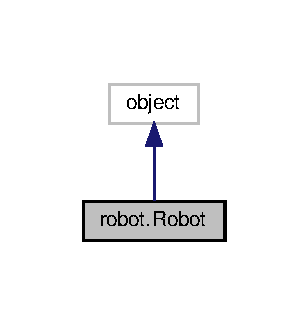
\includegraphics[width=148pt]{classrobot_1_1Robot__inherit__graph}
\end{center}
\end{figure}


Collaboration diagram for robot.\+Robot\+:
\nopagebreak
\begin{figure}[H]
\begin{center}
\leavevmode
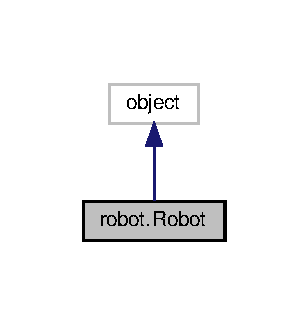
\includegraphics[width=148pt]{classrobot_1_1Robot__coll__graph}
\end{center}
\end{figure}
\subsection*{Public Member Functions}
\begin{DoxyCompactItemize}
\item 
\mbox{\Hypertarget{classrobot_1_1Robot_ad15eeb92007e66802fabd5ce42add7b0}\label{classrobot_1_1Robot_ad15eeb92007e66802fabd5ce42add7b0}} 
def {\bfseries \+\_\+\+\_\+init\+\_\+\+\_\+} (self, name, device=None, tracer=None)
\item 
\mbox{\Hypertarget{classrobot_1_1Robot_a01b3eaee0bfc2251d32aceb7defb858b}\label{classrobot_1_1Robot_a01b3eaee0bfc2251d32aceb7defb858b}} 
def {\bfseries \+\_\+\+\_\+del\+\_\+\+\_\+} (self)
\item 
\mbox{\Hypertarget{classrobot_1_1Robot_afe20b6b2c337dd9e0b4a53ed30c1a0cc}\label{classrobot_1_1Robot_afe20b6b2c337dd9e0b4a53ed30c1a0cc}} 
def {\bfseries add\+\_\+trace} (self, entity\+Name, signal\+Name)
\item 
\mbox{\Hypertarget{classrobot_1_1Robot_a1d39e4c3dd75c6c7592eeafe6596b773}\label{classrobot_1_1Robot_a1d39e4c3dd75c6c7592eeafe6596b773}} 
def {\bfseries initialize\+\_\+tracer} (self)
\item 
\mbox{\Hypertarget{classrobot_1_1Robot_a3efb51e990f1e3292f321858e9a9723f}\label{classrobot_1_1Robot_a3efb51e990f1e3292f321858e9a9723f}} 
def \hyperlink{classrobot_1_1Robot_a3efb51e990f1e3292f321858e9a9723f}{start\+\_\+tracer} (self)
\begin{DoxyCompactList}\small\item\em Start the tracer if it has not already been stopped. \end{DoxyCompactList}\item 
\mbox{\Hypertarget{classrobot_1_1Robot_ace42b97e31dcc38be3bd69b2ab33a214}\label{classrobot_1_1Robot_ace42b97e31dcc38be3bd69b2ab33a214}} 
def \hyperlink{classrobot_1_1Robot_ace42b97e31dcc38be3bd69b2ab33a214}{stop\+\_\+tracer} (self)
\begin{DoxyCompactList}\small\item\em Stop and destroy tracer. \end{DoxyCompactList}\item 
\mbox{\Hypertarget{classrobot_1_1Robot_ac208f7eafdff6ad891e77402167e9ccc}\label{classrobot_1_1Robot_ac208f7eafdff6ad891e77402167e9ccc}} 
def {\bfseries add\+\_\+to\+\_\+ros} (self, entity\+Name, signal\+Name, topic\+\_\+name=None, topic\+\_\+type=None)
\item 
\mbox{\Hypertarget{classrobot_1_1Robot_a6c8b057c894e762bb43ceb7ec3e7db35}\label{classrobot_1_1Robot_a6c8b057c894e762bb43ceb7ec3e7db35}} 
def {\bfseries add\+\_\+robot\+\_\+state\+\_\+to\+\_\+ros} (self, entity\+\_\+name, signal\+\_\+name, base\+\_\+link\+\_\+name, joint\+\_\+names, tf\+\_\+prefix, joint\+\_\+state\+\_\+topic\+\_\+name)
\item 
\mbox{\Hypertarget{classrobot_1_1Robot_a737de35c18b3bf050dc477da3a841970}\label{classrobot_1_1Robot_a737de35c18b3bf050dc477da3a841970}} 
def {\bfseries add\+\_\+ros\+\_\+and\+\_\+trace} (self, entity\+Name, signal\+Name, topic\+\_\+name=None, topic\+\_\+type=None)
\item 
\mbox{\Hypertarget{classrobot_1_1Robot_ad5787c862823008387c047da5f34dd7e}\label{classrobot_1_1Robot_ad5787c862823008387c047da5f34dd7e}} 
def \hyperlink{classrobot_1_1Robot_ad5787c862823008387c047da5f34dd7e}{export\+\_\+device\+\_\+dg\+\_\+to\+\_\+ros} (self)
\begin{DoxyCompactList}\small\item\em Import in R\+OS the signal from the dynamic graph device. \end{DoxyCompactList}\end{DoxyCompactItemize}
\subsection*{Public Attributes}
\begin{DoxyCompactItemize}
\item 
\mbox{\Hypertarget{classrobot_1_1Robot_a24273c64e4c3266dd075ead7cd570c58}\label{classrobot_1_1Robot_a24273c64e4c3266dd075ead7cd570c58}} 
{\bfseries name}
\item 
\mbox{\Hypertarget{classrobot_1_1Robot_ae90b19f45d0f60f5a9bcae2b96214ce7}\label{classrobot_1_1Robot_ae90b19f45d0f60f5a9bcae2b96214ce7}} 
{\bfseries device}
\item 
\mbox{\Hypertarget{classrobot_1_1Robot_a76c94351e17cf2da6a47f594db60bb14}\label{classrobot_1_1Robot_a76c94351e17cf2da6a47f594db60bb14}} 
{\bfseries device\+\_\+signals\+\_\+names}
\item 
\mbox{\Hypertarget{classrobot_1_1Robot_aa64d4907ff7bc8916ab94993e36e8e92}\label{classrobot_1_1Robot_aa64d4907ff7bc8916ab94993e36e8e92}} 
{\bfseries ros}
\item 
\mbox{\Hypertarget{classrobot_1_1Robot_a64ffbcaa3fa142fc15fb928f0a171609}\label{classrobot_1_1Robot_a64ffbcaa3fa142fc15fb928f0a171609}} 
{\bfseries tracer\+\_\+log\+\_\+dir}
\item 
\mbox{\Hypertarget{classrobot_1_1Robot_aafc575f3ec8bd5a21277cca9645df962}\label{classrobot_1_1Robot_aafc575f3ec8bd5a21277cca9645df962}} 
{\bfseries trace}
\end{DoxyCompactItemize}
\subsection*{Static Public Attributes}
\begin{DoxyCompactItemize}
\item 
\mbox{\Hypertarget{classrobot_1_1Robot_a72835f96d0dfcdfe1b2d4feddfa727d2}\label{classrobot_1_1Robot_a72835f96d0dfcdfe1b2d4feddfa727d2}} 
tuple {\bfseries init\+\_\+pos} = (0.\+0)
\item 
\mbox{\Hypertarget{classrobot_1_1Robot_ab50d0c91e1751573073a937ef9df4dad}\label{classrobot_1_1Robot_ab50d0c91e1751573073a937ef9df4dad}} 
tuple {\bfseries init\+\_\+vel} = (0.\+0)
\item 
\mbox{\Hypertarget{classrobot_1_1Robot_ada231c72c7967d3f61083316224fa965}\label{classrobot_1_1Robot_ada231c72c7967d3f61083316224fa965}} 
tuple {\bfseries init\+\_\+acc} = (0.\+0)
\item 
\mbox{\Hypertarget{classrobot_1_1Robot_adda6f00aaeb6562a2cc9d682cbcdb478}\label{classrobot_1_1Robot_adda6f00aaeb6562a2cc9d682cbcdb478}} 
{\bfseries tracer} = None
\item 
\mbox{\Hypertarget{classrobot_1_1Robot_a29af80c65f6ad9e61fae2cf76d81b9e0}\label{classrobot_1_1Robot_a29af80c65f6ad9e61fae2cf76d81b9e0}} 
int {\bfseries tracer\+Size} = 2$\ast$$\ast$22
\item 
\mbox{\Hypertarget{classrobot_1_1Robot_ab11ca34e29d7aac471df46b6fe56e7a9}\label{classrobot_1_1Robot_ab11ca34e29d7aac471df46b6fe56e7a9}} 
list {\bfseries auto\+Recomputed\+Signals} = \mbox{[}$\,$\mbox{]}
\item 
\mbox{\Hypertarget{classrobot_1_1Robot_a4e690827b25920c0088890fbeea1667b}\label{classrobot_1_1Robot_a4e690827b25920c0088890fbeea1667b}} 
float {\bfseries time\+Step} = 0.\+005
\end{DoxyCompactItemize}
\subsection*{Private Member Functions}
\begin{DoxyCompactItemize}
\item 
\mbox{\Hypertarget{classrobot_1_1Robot_a4c9fe65c4c794832943aaa7f5ca76a09}\label{classrobot_1_1Robot_a4c9fe65c4c794832943aaa7f5ca76a09}} 
def {\bfseries \+\_\+tracer\+\_\+log\+\_\+dir} (self)
\end{DoxyCompactItemize}


\subsection{Detailed Description}
This class instantiates a robot. 

The documentation for this class was generated from the following file\+:\begin{DoxyCompactItemize}
\item 
python/dynamic\+\_\+graph\+\_\+manager/device/\hyperlink{robot_8py}{robot.\+py}\end{DoxyCompactItemize}

\hypertarget{classros_1_1ros_1_1Ros}{}\section{ros.\+ros.\+Ros Class Reference}
\label{classros_1_1ros_1_1Ros}\index{ros.\+ros.\+Ros@{ros.\+ros.\+Ros}}


Inheritance diagram for ros.\+ros.\+Ros\+:
\nopagebreak
\begin{figure}[H]
\begin{center}
\leavevmode
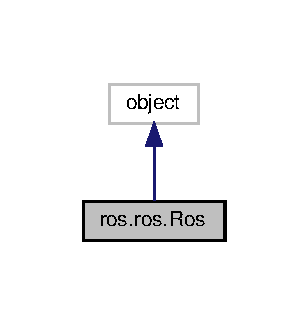
\includegraphics[width=148pt]{classros_1_1ros_1_1Ros__inherit__graph}
\end{center}
\end{figure}


Collaboration diagram for ros.\+ros.\+Ros\+:
\nopagebreak
\begin{figure}[H]
\begin{center}
\leavevmode
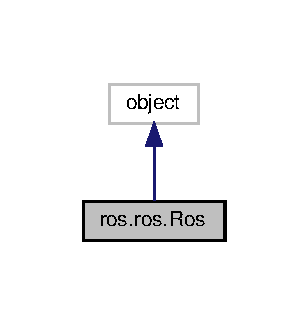
\includegraphics[width=148pt]{classros_1_1ros_1_1Ros__coll__graph}
\end{center}
\end{figure}
\subsection*{Public Member Functions}
\begin{DoxyCompactItemize}
\item 
\mbox{\Hypertarget{classros_1_1ros_1_1Ros_afc21e7cd18df42d888198438e6a0fe6d}\label{classros_1_1ros_1_1Ros_afc21e7cd18df42d888198438e6a0fe6d}} 
def {\bfseries \+\_\+\+\_\+init\+\_\+\+\_\+} (self, robot, suffix=\textquotesingle{}\textquotesingle{})
\end{DoxyCompactItemize}
\subsection*{Public Attributes}
\begin{DoxyCompactItemize}
\item 
\mbox{\Hypertarget{classros_1_1ros_1_1Ros_a0befef81b5386c7b5b1ca0d13d0d2a64}\label{classros_1_1ros_1_1Ros_a0befef81b5386c7b5b1ca0d13d0d2a64}} 
{\bfseries robot}
\item 
\mbox{\Hypertarget{classros_1_1ros_1_1Ros_a2ddca71f44605c7268029a374070d64b}\label{classros_1_1ros_1_1Ros_a2ddca71f44605c7268029a374070d64b}} 
{\bfseries ros\+Publish}
\item 
\mbox{\Hypertarget{classros_1_1ros_1_1Ros_a31ff2a70df03c3a0283e4b8a17c019e2}\label{classros_1_1ros_1_1Ros_a31ff2a70df03c3a0283e4b8a17c019e2}} 
{\bfseries ros\+Subscribe}
\item 
\mbox{\Hypertarget{classros_1_1ros_1_1Ros_a323ae5f5e4205f31f1bda8424bf534e6}\label{classros_1_1ros_1_1Ros_a323ae5f5e4205f31f1bda8424bf534e6}} 
{\bfseries ros\+Time}
\item 
\mbox{\Hypertarget{classros_1_1ros_1_1Ros_ae35fd5139c151671b1134f4725cbcc33}\label{classros_1_1ros_1_1Ros_ae35fd5139c151671b1134f4725cbcc33}} 
{\bfseries ros\+Robot\+State\+Publisher}
\item 
\mbox{\Hypertarget{classros_1_1ros_1_1Ros_adaf7ed0ec413adea74e298742c34b36a}\label{classros_1_1ros_1_1Ros_adaf7ed0ec413adea74e298742c34b36a}} 
{\bfseries ros\+Import}
\item 
\mbox{\Hypertarget{classros_1_1ros_1_1Ros_a9631d40df4f07890316cead5a94876a3}\label{classros_1_1ros_1_1Ros_a9631d40df4f07890316cead5a94876a3}} 
{\bfseries ros\+Export}
\end{DoxyCompactItemize}


The documentation for this class was generated from the following file\+:\begin{DoxyCompactItemize}
\item 
python/dynamic\+\_\+graph\+\_\+manager/ros/\hyperlink{ros_8py}{ros.\+py}\end{DoxyCompactItemize}

\hypertarget{classdynamic__graph_1_1RosPublish}{}\section{dynamic\+\_\+graph\+:\+:Ros\+Publish Class Reference}
\label{classdynamic__graph_1_1RosPublish}\index{dynamic\+\_\+graph\+::\+Ros\+Publish@{dynamic\+\_\+graph\+::\+Ros\+Publish}}


Publish dynamic-\/graph information into R\+OS.  




{\ttfamily \#include $<$ros\+\_\+publish.\+hh$>$}



Inheritance diagram for dynamic\+\_\+graph\+:\+:Ros\+Publish\+:\nopagebreak
\begin{figure}[H]
\begin{center}
\leavevmode
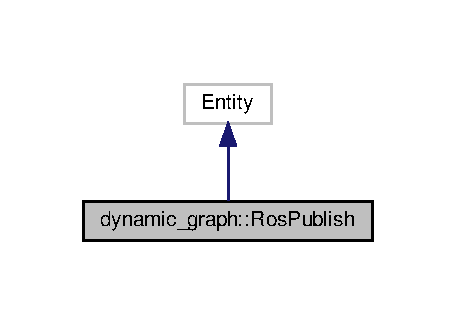
\includegraphics[width=219pt]{classdynamic__graph_1_1RosPublish__inherit__graph}
\end{center}
\end{figure}


Collaboration diagram for dynamic\+\_\+graph\+:\+:Ros\+Publish\+:\nopagebreak
\begin{figure}[H]
\begin{center}
\leavevmode
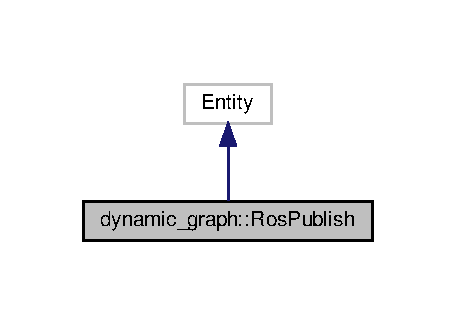
\includegraphics[width=219pt]{classdynamic__graph_1_1RosPublish__coll__graph}
\end{center}
\end{figure}
\subsection*{Public Types}
\begin{DoxyCompactItemize}
\item 
typedef boost\+::function$<$ void(int)$>$ {\bfseries callback\+\_\+t}\hypertarget{classdynamic__graph_1_1RosPublish_a93af27416b602041eaf6f639d9219a60}{}\label{classdynamic__graph_1_1RosPublish_a93af27416b602041eaf6f639d9219a60}

\item 
typedef boost\+::tuple$<$ boost\+::shared\+\_\+ptr$<$ dynamicgraph\+::\+Signal\+Base$<$ int $>$ $>$, callback\+\_\+t $>$ {\bfseries binded\+Signal\+\_\+t}\hypertarget{classdynamic__graph_1_1RosPublish_a5a2727a6ffd99a30102448dc05381593}{}\label{classdynamic__graph_1_1RosPublish_a5a2727a6ffd99a30102448dc05381593}

\end{DoxyCompactItemize}
\subsection*{Public Member Functions}
\begin{DoxyCompactItemize}
\item 
{\bfseries Ros\+Publish} (const std\+::string \&n)\hypertarget{classdynamic__graph_1_1RosPublish_a096779c4bfebb42570b99522a0080cd7}{}\label{classdynamic__graph_1_1RosPublish_a096779c4bfebb42570b99522a0080cd7}

\item 
virtual std\+::string {\bfseries get\+Doc\+String} () const \hypertarget{classdynamic__graph_1_1RosPublish_a0e0678abe0a8daf396cb979f7b36fdc7}{}\label{classdynamic__graph_1_1RosPublish_a0e0678abe0a8daf396cb979f7b36fdc7}

\item 
void {\bfseries display} (std\+::ostream \&os) const \hypertarget{classdynamic__graph_1_1RosPublish_a31a960cdd57d1627cbd192ae179132a0}{}\label{classdynamic__graph_1_1RosPublish_a31a960cdd57d1627cbd192ae179132a0}

\item 
void {\bfseries add} (const std\+::string \&signal, const std\+::string \&topic)\hypertarget{classdynamic__graph_1_1RosPublish_ad0e751d0df273d7b35a39802cfd2e2f4}{}\label{classdynamic__graph_1_1RosPublish_ad0e751d0df273d7b35a39802cfd2e2f4}

\item 
void {\bfseries rm} (const std\+::string \&signal)\hypertarget{classdynamic__graph_1_1RosPublish_acfc49e5212dc48c7623b10d4b48be8ad}{}\label{classdynamic__graph_1_1RosPublish_acfc49e5212dc48c7623b10d4b48be8ad}

\item 
std\+::string {\bfseries list} () const \hypertarget{classdynamic__graph_1_1RosPublish_a26a60355631c7df2364cbb7f8309c467}{}\label{classdynamic__graph_1_1RosPublish_a26a60355631c7df2364cbb7f8309c467}

\item 
void {\bfseries clear} ()\hypertarget{classdynamic__graph_1_1RosPublish_a3e6ddd8230db25e46874193b81f31715}{}\label{classdynamic__graph_1_1RosPublish_a3e6ddd8230db25e46874193b81f31715}

\item 
int \& {\bfseries trigger} (int \&, int)\hypertarget{classdynamic__graph_1_1RosPublish_aedf99adaa287e141875b3061c2699c64}{}\label{classdynamic__graph_1_1RosPublish_aedf99adaa287e141875b3061c2699c64}

\item 
{\footnotesize template$<$typename T $>$ }\\void {\bfseries send\+Data} (boost\+::shared\+\_\+ptr$<$ realtime\+\_\+tools\+::\+Realtime\+Publisher$<$ typename \hyperlink{classdynamic__graph_1_1DgToRos}{Dg\+To\+Ros}$<$ T $>$\+::ros\+\_\+t $>$ $>$ publisher, boost\+::shared\+\_\+ptr$<$ typename \hyperlink{classdynamic__graph_1_1DgToRos}{Dg\+To\+Ros}$<$ T $>$\+::signal\+In\+\_\+t $>$ signal, int time)\hypertarget{classdynamic__graph_1_1RosPublish_a3d0602010171406c481116458ced5211}{}\label{classdynamic__graph_1_1RosPublish_a3d0602010171406c481116458ced5211}

\item 
{\footnotesize template$<$typename T $>$ }\\void {\bfseries add} (const std\+::string \&signal, const std\+::string \&topic)\hypertarget{classdynamic__graph_1_1RosPublish_af77a721d482487d5cf55929ccbbeef96}{}\label{classdynamic__graph_1_1RosPublish_af77a721d482487d5cf55929ccbbeef96}

\end{DoxyCompactItemize}
\subsection*{Static Public Attributes}
\begin{DoxyCompactItemize}
\item 
static const double {\bfseries R\+O\+S\+\_\+\+J\+O\+I\+N\+T\+\_\+\+S\+T\+A\+T\+E\+\_\+\+P\+U\+B\+L\+I\+S\+H\+E\+R\+\_\+\+R\+A\+TE} = 0.\+01\hypertarget{classdynamic__graph_1_1RosPublish_af3ffea00d60088a4b921a8a37b0f405d}{}\label{classdynamic__graph_1_1RosPublish_af3ffea00d60088a4b921a8a37b0f405d}

\end{DoxyCompactItemize}


\subsection{Detailed Description}
Publish dynamic-\/graph information into R\+OS. 

The documentation for this class was generated from the following files\+:\begin{DoxyCompactItemize}
\item 
/home/mnaveau/devel/workspace/src/catkin/dg\+\_\+control/dynamic\+\_\+graph\+\_\+manager/include/ros\+\_\+entities/\hyperlink{ros__publish_8hh}{ros\+\_\+publish.\+hh}\item 
/home/mnaveau/devel/workspace/src/catkin/dg\+\_\+control/dynamic\+\_\+graph\+\_\+manager/src/ros\+\_\+entities/\hyperlink{ros__publish_8cpp}{ros\+\_\+publish.\+cpp}\item 
/home/mnaveau/devel/workspace/src/catkin/dg\+\_\+control/dynamic\+\_\+graph\+\_\+manager/include/ros\+\_\+entities/\hyperlink{ros__publish_8hxx}{ros\+\_\+publish.\+hxx}\end{DoxyCompactItemize}

\hypertarget{classros_1_1ros__client_1_1RosPythonInterpreter}{}\section{ros.\+ros\+\_\+client.\+Ros\+Python\+Interpreter Class Reference}
\label{classros_1_1ros__client_1_1RosPythonInterpreter}\index{ros.\+ros\+\_\+client.\+Ros\+Python\+Interpreter@{ros.\+ros\+\_\+client.\+Ros\+Python\+Interpreter}}


Inheritance diagram for ros.\+ros\+\_\+client.\+Ros\+Python\+Interpreter\+:
\nopagebreak
\begin{figure}[H]
\begin{center}
\leavevmode
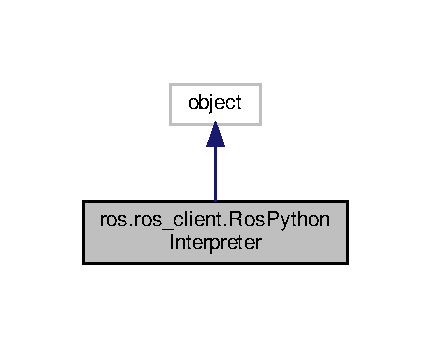
\includegraphics[width=207pt]{classros_1_1ros__client_1_1RosPythonInterpreter__inherit__graph}
\end{center}
\end{figure}


Collaboration diagram for ros.\+ros\+\_\+client.\+Ros\+Python\+Interpreter\+:
\nopagebreak
\begin{figure}[H]
\begin{center}
\leavevmode
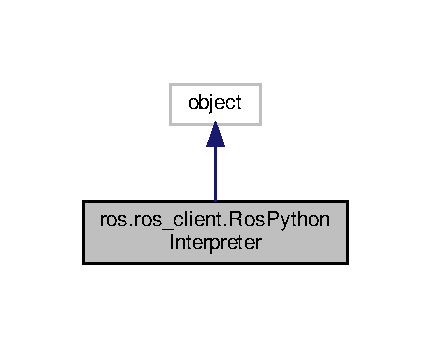
\includegraphics[width=207pt]{classros_1_1ros__client_1_1RosPythonInterpreter__coll__graph}
\end{center}
\end{figure}
\subsection*{Public Member Functions}
\begin{DoxyCompactItemize}
\item 
def {\bfseries \+\_\+\+\_\+init\+\_\+\+\_\+} (self)\hypertarget{classros_1_1ros__client_1_1RosPythonInterpreter_abdeeebfed829bcb91f8f5fe195b6bdc9}{}\label{classros_1_1ros__client_1_1RosPythonInterpreter_abdeeebfed829bcb91f8f5fe195b6bdc9}

\item 
def \hyperlink{classros_1_1ros__client_1_1RosPythonInterpreter_ad1de2f9fb464e1f3f81dbac5396208f7}{run\+\_\+python\+\_\+command} (self, code\+\_\+string)\hypertarget{classros_1_1ros__client_1_1RosPythonInterpreter_ad1de2f9fb464e1f3f81dbac5396208f7}{}\label{classros_1_1ros__client_1_1RosPythonInterpreter_ad1de2f9fb464e1f3f81dbac5396208f7}

\begin{DoxyCompactList}\small\item\em Call the rosservice of the current running dynamic graph manager. \end{DoxyCompactList}\item 
def \hyperlink{classros_1_1ros__client_1_1RosPythonInterpreter_a63e042101395102abd40958406bea3a2}{run\+\_\+python\+\_\+script} (self, filename)\hypertarget{classros_1_1ros__client_1_1RosPythonInterpreter_a63e042101395102abd40958406bea3a2}{}\label{classros_1_1ros__client_1_1RosPythonInterpreter_a63e042101395102abd40958406bea3a2}

\begin{DoxyCompactList}\small\item\em Call the rosservice of the current running dynamic graph manager. \end{DoxyCompactList}\end{DoxyCompactItemize}
\subsection*{Public Attributes}
\begin{DoxyCompactItemize}
\item 
{\bfseries run\+\_\+command\+\_\+service\+\_\+name}\hypertarget{classros_1_1ros__client_1_1RosPythonInterpreter_a36cd3a0e3570dbfde5ced42607bb9367}{}\label{classros_1_1ros__client_1_1RosPythonInterpreter_a36cd3a0e3570dbfde5ced42607bb9367}

\item 
{\bfseries command\+\_\+client}\hypertarget{classros_1_1ros__client_1_1RosPythonInterpreter_aea957df856e6fe9ad8c471b2c382ebab}{}\label{classros_1_1ros__client_1_1RosPythonInterpreter_aea957df856e6fe9ad8c471b2c382ebab}

\item 
{\bfseries run\+\_\+script\+\_\+service\+\_\+name}\hypertarget{classros_1_1ros__client_1_1RosPythonInterpreter_ab93db3a217d257a6c50d944bd1edb43a}{}\label{classros_1_1ros__client_1_1RosPythonInterpreter_ab93db3a217d257a6c50d944bd1edb43a}

\item 
{\bfseries script\+\_\+client}\hypertarget{classros_1_1ros__client_1_1RosPythonInterpreter_a17bb95376765347cd27c645b3399f071}{}\label{classros_1_1ros__client_1_1RosPythonInterpreter_a17bb95376765347cd27c645b3399f071}

\item 
{\bfseries timeout\+\_\+connection}\hypertarget{classros_1_1ros__client_1_1RosPythonInterpreter_abce1abc9d628db983be2ed02522550d1}{}\label{classros_1_1ros__client_1_1RosPythonInterpreter_abce1abc9d628db983be2ed02522550d1}

\end{DoxyCompactItemize}
\subsection*{Private Member Functions}
\begin{DoxyCompactItemize}
\item 
def {\bfseries \+\_\+connect\+\_\+to\+\_\+rosservice\+\_\+run\+\_\+python\+\_\+command} (self, timeout=None)\hypertarget{classros_1_1ros__client_1_1RosPythonInterpreter_a443b997ed6c8f6a0bea05aae15403686}{}\label{classros_1_1ros__client_1_1RosPythonInterpreter_a443b997ed6c8f6a0bea05aae15403686}

\item 
def {\bfseries \+\_\+connect\+\_\+to\+\_\+rosservice\+\_\+run\+\_\+python\+\_\+script} (self, timeout=None)\hypertarget{classros_1_1ros__client_1_1RosPythonInterpreter_a051256d44254766bd342d5f68f30b454}{}\label{classros_1_1ros__client_1_1RosPythonInterpreter_a051256d44254766bd342d5f68f30b454}

\item 
def \hyperlink{classros_1_1ros__client_1_1RosPythonInterpreter_a817a0c056aeeba19895cb8c111c370df}{\+\_\+atexit} (self)\hypertarget{classros_1_1ros__client_1_1RosPythonInterpreter_a817a0c056aeeba19895cb8c111c370df}{}\label{classros_1_1ros__client_1_1RosPythonInterpreter_a817a0c056aeeba19895cb8c111c370df}

\begin{DoxyCompactList}\small\item\em Execute a couple of instruction upon exit. \end{DoxyCompactList}\end{DoxyCompactItemize}
\subsection*{Static Private Member Functions}
\begin{DoxyCompactItemize}
\item 
def {\bfseries \+\_\+connect\+\_\+to\+\_\+rosservice} (service\+\_\+name, rosservice, timeout)\hypertarget{classros_1_1ros__client_1_1RosPythonInterpreter_a8a6ff47e74db5c036872d3628957c9d0}{}\label{classros_1_1ros__client_1_1RosPythonInterpreter_a8a6ff47e74db5c036872d3628957c9d0}

\end{DoxyCompactItemize}


The documentation for this class was generated from the following file\+:\begin{DoxyCompactItemize}
\item 
python/dynamic\+\_\+graph\+\_\+manager/ros/\hyperlink{ros__client_8py}{ros\+\_\+client.\+py}\end{DoxyCompactItemize}

\hypertarget{classdynamic__graph_1_1RosPythonInterpreter}{}\section{dynamic\+\_\+graph\+:\+:Ros\+Python\+Interpreter Class Reference}
\label{classdynamic__graph_1_1RosPythonInterpreter}\index{dynamic\+\_\+graph\+::\+Ros\+Python\+Interpreter@{dynamic\+\_\+graph\+::\+Ros\+Python\+Interpreter}}


This class wraps the implementation of the run\+Command service.  




{\ttfamily \#include $<$ros\+\_\+interpreter.\+hh$>$}

\subsection*{Public Types}
\begin{DoxyCompactItemize}
\item 
typedef boost\+::function$<$ bool(dynamic\+\_\+graph\+\_\+manager\+::\+Run\+Command\+::\+Request \&, dynamic\+\_\+graph\+\_\+manager\+::\+Run\+Command\+::\+Response \&)$>$ \hyperlink{classdynamic__graph_1_1RosPythonInterpreter_aa9fcb34973d84db722fa39803d11c00d}{run\+\_\+python\+\_\+command\+\_\+callback\+\_\+t}
\begin{DoxyCompactList}\small\item\em run\+\_\+python\+\_\+command\+\_\+callback\+\_\+t define a boost\+::function to be used as callback to the ros\+::service. \end{DoxyCompactList}\item 
typedef boost\+::function$<$ bool(dynamic\+\_\+graph\+\_\+manager\+::\+Run\+Python\+File\+::\+Request \&, dynamic\+\_\+graph\+\_\+manager\+::\+Run\+Python\+File\+::\+Response \&)$>$ \hyperlink{classdynamic__graph_1_1RosPythonInterpreter_a802128e670817aa48dd8db54830a7977}{run\+\_\+python\+\_\+file\+\_\+callback\+\_\+t}
\begin{DoxyCompactList}\small\item\em run\+\_\+python\+\_\+file\+\_\+callback\+\_\+t define a boost\+::function to be used as callback to the ros\+::service. \end{DoxyCompactList}\end{DoxyCompactItemize}
\subsection*{Public Member Functions}
\begin{DoxyCompactItemize}
\item 
\hyperlink{classdynamic__graph_1_1RosPythonInterpreter_a082493a5a7edd758b65a34fc9e617df5}{Ros\+Python\+Interpreter} (ros\+::\+Node\+Handle \&node\+\_\+handle)
\begin{DoxyCompactList}\small\item\em \hyperlink{classdynamic__graph_1_1RosPythonInterpreter}{Ros\+Python\+Interpreter} is the unique constructor of the class. \end{DoxyCompactList}\item 
\hyperlink{classdynamic__graph_1_1RosPythonInterpreter_a45378e164f35c3cc8dffe1cca7473dde}{$\sim$\+Ros\+Python\+Interpreter} ()\hypertarget{classdynamic__graph_1_1RosPythonInterpreter_a45378e164f35c3cc8dffe1cca7473dde}{}\label{classdynamic__graph_1_1RosPythonInterpreter_a45378e164f35c3cc8dffe1cca7473dde}

\begin{DoxyCompactList}\small\item\em $\sim$\+Ros\+Python\+Interpreter is the default destructor of the class \end{DoxyCompactList}\item 
void \hyperlink{classdynamic__graph_1_1RosPythonInterpreter_a9745742713e7dc9302468519c1cae9a1}{run\+\_\+python\+\_\+command} (const std\+::string \&command, std\+::string \&result, std\+::string \&out, std\+::string \&err)
\begin{DoxyCompactList}\small\item\em run\+\_\+python\+\_\+command used the python interpreter to execute the input command \end{DoxyCompactList}\item 
void \hyperlink{classdynamic__graph_1_1RosPythonInterpreter_a4a90b557973b8aa533e297adab4bcbe6}{run\+\_\+python\+\_\+file} (const std\+::string ifilename, std\+::string \&standard\+\_\+error)
\begin{DoxyCompactList}\small\item\em run\+\_\+python\+\_\+file executes the input scripts in the python interpreter \end{DoxyCompactList}\item 
void \hyperlink{classdynamic__graph_1_1RosPythonInterpreter_ae6f58ecea63921945529f367c27dd70e}{start\+\_\+ros\+\_\+service} ()\hypertarget{classdynamic__graph_1_1RosPythonInterpreter_ae6f58ecea63921945529f367c27dd70e}{}\label{classdynamic__graph_1_1RosPythonInterpreter_ae6f58ecea63921945529f367c27dd70e}

\begin{DoxyCompactList}\small\item\em start\+\_\+ros\+\_\+service advertize the \char`\"{}run\+\_\+python\+\_\+command\char`\"{} and \char`\"{}run\+\_\+python\+\_\+scripts\char`\"{} ros services \end{DoxyCompactList}\end{DoxyCompactItemize}
\subsection*{Protected Member Functions}
\begin{DoxyCompactItemize}
\item 
bool \hyperlink{classdynamic__graph_1_1RosPythonInterpreter_af589eb361f3193c48c7e7f2eb5a3ff64}{run\+Command\+Callback} (dynamic\+\_\+graph\+\_\+manager\+::\+Run\+Command\+::\+Request \&req, dynamic\+\_\+graph\+\_\+manager\+::\+Run\+Command\+::\+Response \&res)
\begin{DoxyCompactList}\small\item\em run\+Command\+Callback is the \char`\"{}run\+\_\+python\+\_\+command\char`\"{} ros service callback function. \end{DoxyCompactList}\item 
bool \hyperlink{classdynamic__graph_1_1RosPythonInterpreter_a519321128872afdcec622a4892c63196}{run\+Python\+File\+Callback} (dynamic\+\_\+graph\+\_\+manager\+::\+Run\+Python\+File\+::\+Request \&req, dynamic\+\_\+graph\+\_\+manager\+::\+Run\+Python\+File\+::\+Response \&res)
\begin{DoxyCompactList}\small\item\em run\+Command\+Callback is the \char`\"{}run\+\_\+python\+\_\+script\char`\"{} ros service callback function. \end{DoxyCompactList}\end{DoxyCompactItemize}


\subsection{Detailed Description}
This class wraps the implementation of the run\+Command service. 

This takes as input a R\+OS node handle and do not handle the callback so that the service behavior can be controlled from the outside. 

\subsection{Member Typedef Documentation}
\index{dynamic\+\_\+graph\+::\+Ros\+Python\+Interpreter@{dynamic\+\_\+graph\+::\+Ros\+Python\+Interpreter}!run\+\_\+python\+\_\+command\+\_\+callback\+\_\+t@{run\+\_\+python\+\_\+command\+\_\+callback\+\_\+t}}
\index{run\+\_\+python\+\_\+command\+\_\+callback\+\_\+t@{run\+\_\+python\+\_\+command\+\_\+callback\+\_\+t}!dynamic\+\_\+graph\+::\+Ros\+Python\+Interpreter@{dynamic\+\_\+graph\+::\+Ros\+Python\+Interpreter}}
\subsubsection[{\texorpdfstring{run\+\_\+python\+\_\+command\+\_\+callback\+\_\+t}{run_python_command_callback_t}}]{\setlength{\rightskip}{0pt plus 5cm}typedef boost\+::function$<$ bool (dynamic\+\_\+graph\+\_\+manager\+::\+Run\+Command\+::\+Request\&, dynamic\+\_\+graph\+\_\+manager\+::\+Run\+Command\+::\+Response\&)$>$ {\bf dynamic\+\_\+graph\+::\+Ros\+Python\+Interpreter\+::run\+\_\+python\+\_\+command\+\_\+callback\+\_\+t}}\hypertarget{classdynamic__graph_1_1RosPythonInterpreter_aa9fcb34973d84db722fa39803d11c00d}{}\label{classdynamic__graph_1_1RosPythonInterpreter_aa9fcb34973d84db722fa39803d11c00d}


run\+\_\+python\+\_\+command\+\_\+callback\+\_\+t define a boost\+::function to be used as callback to the ros\+::service. 

The first argument of \char`\"{}run\+Command\+Callback\char`\"{} (const std\+::string \& command) is bound to (dynamic\+\_\+graph\+\_\+manager\+::\+Run\+Command\+::\+Request). And the second argument (std\+::string \&result) is bound to (dynamic\+\_\+graph\+\_\+manager\+::\+Run\+Command\+::\+Response) \index{dynamic\+\_\+graph\+::\+Ros\+Python\+Interpreter@{dynamic\+\_\+graph\+::\+Ros\+Python\+Interpreter}!run\+\_\+python\+\_\+file\+\_\+callback\+\_\+t@{run\+\_\+python\+\_\+file\+\_\+callback\+\_\+t}}
\index{run\+\_\+python\+\_\+file\+\_\+callback\+\_\+t@{run\+\_\+python\+\_\+file\+\_\+callback\+\_\+t}!dynamic\+\_\+graph\+::\+Ros\+Python\+Interpreter@{dynamic\+\_\+graph\+::\+Ros\+Python\+Interpreter}}
\subsubsection[{\texorpdfstring{run\+\_\+python\+\_\+file\+\_\+callback\+\_\+t}{run_python_file_callback_t}}]{\setlength{\rightskip}{0pt plus 5cm}typedef boost\+::function$<$ bool (dynamic\+\_\+graph\+\_\+manager\+::\+Run\+Python\+File\+::\+Request\&, dynamic\+\_\+graph\+\_\+manager\+::\+Run\+Python\+File\+::\+Response\&)$>$ {\bf dynamic\+\_\+graph\+::\+Ros\+Python\+Interpreter\+::run\+\_\+python\+\_\+file\+\_\+callback\+\_\+t}}\hypertarget{classdynamic__graph_1_1RosPythonInterpreter_a802128e670817aa48dd8db54830a7977}{}\label{classdynamic__graph_1_1RosPythonInterpreter_a802128e670817aa48dd8db54830a7977}


run\+\_\+python\+\_\+file\+\_\+callback\+\_\+t define a boost\+::function to be used as callback to the ros\+::service. 

The first argument of \char`\"{}run\+Python\+File\+Callback\char`\"{} (std\+::string ifilename) is bound to (dynamic\+\_\+graph\+\_\+manager\+::\+Run\+Command\+::\+Request). And a fake second argument is simulated in (dynamic\+\_\+graph\+\_\+manager\+::\+Run\+Command\+::\+Response) 

\subsection{Constructor \& Destructor Documentation}
\index{dynamic\+\_\+graph\+::\+Ros\+Python\+Interpreter@{dynamic\+\_\+graph\+::\+Ros\+Python\+Interpreter}!Ros\+Python\+Interpreter@{Ros\+Python\+Interpreter}}
\index{Ros\+Python\+Interpreter@{Ros\+Python\+Interpreter}!dynamic\+\_\+graph\+::\+Ros\+Python\+Interpreter@{dynamic\+\_\+graph\+::\+Ros\+Python\+Interpreter}}
\subsubsection[{\texorpdfstring{Ros\+Python\+Interpreter(ros\+::\+Node\+Handle \&node\+\_\+handle)}{RosPythonInterpreter(ros::NodeHandle &node_handle)}}]{\setlength{\rightskip}{0pt plus 5cm}dynamic\+\_\+graph\+::\+Ros\+Python\+Interpreter\+::\+Ros\+Python\+Interpreter (
\begin{DoxyParamCaption}
\item[{ros\+::\+Node\+Handle \&}]{node\+\_\+handle}
\end{DoxyParamCaption}
)\hspace{0.3cm}{\ttfamily [explicit]}}\hypertarget{classdynamic__graph_1_1RosPythonInterpreter_a082493a5a7edd758b65a34fc9e617df5}{}\label{classdynamic__graph_1_1RosPythonInterpreter_a082493a5a7edd758b65a34fc9e617df5}


\hyperlink{classdynamic__graph_1_1RosPythonInterpreter}{Ros\+Python\+Interpreter} is the unique constructor of the class. 


\begin{DoxyParams}{Parameters}
{\em node\+\_\+handle} & is the ros\+::node\+Handle used to advertize the ros\+::services \\
\hline
\end{DoxyParams}


\subsection{Member Function Documentation}
\index{dynamic\+\_\+graph\+::\+Ros\+Python\+Interpreter@{dynamic\+\_\+graph\+::\+Ros\+Python\+Interpreter}!run\+\_\+python\+\_\+command@{run\+\_\+python\+\_\+command}}
\index{run\+\_\+python\+\_\+command@{run\+\_\+python\+\_\+command}!dynamic\+\_\+graph\+::\+Ros\+Python\+Interpreter@{dynamic\+\_\+graph\+::\+Ros\+Python\+Interpreter}}
\subsubsection[{\texorpdfstring{run\+\_\+python\+\_\+command(const std\+::string \&command, std\+::string \&result, std\+::string \&out, std\+::string \&err)}{run_python_command(const std::string &command, std::string &result, std::string &out, std::string &err)}}]{\setlength{\rightskip}{0pt plus 5cm}void dynamic\+\_\+graph\+::\+Ros\+Python\+Interpreter\+::run\+\_\+python\+\_\+command (
\begin{DoxyParamCaption}
\item[{const std\+::string \&}]{command, }
\item[{std\+::string \&}]{result, }
\item[{std\+::string \&}]{out, }
\item[{std\+::string \&}]{err}
\end{DoxyParamCaption}
)}\hypertarget{classdynamic__graph_1_1RosPythonInterpreter_a9745742713e7dc9302468519c1cae9a1}{}\label{classdynamic__graph_1_1RosPythonInterpreter_a9745742713e7dc9302468519c1cae9a1}


run\+\_\+python\+\_\+command used the python interpreter to execute the input command 


\begin{DoxyParams}[1]{Parameters}
\mbox{\tt in}  & {\em command} & is the user input string command. \\
\hline
\mbox{\tt out}  & {\em result} & is the numerical result of the operation done. \\
\hline
\mbox{\tt out}  & {\em out} & is the string representation of the results. \\
\hline
\mbox{\tt out}  & {\em err} & is the output error string from python. \\
\hline
\end{DoxyParams}
\index{dynamic\+\_\+graph\+::\+Ros\+Python\+Interpreter@{dynamic\+\_\+graph\+::\+Ros\+Python\+Interpreter}!run\+\_\+python\+\_\+file@{run\+\_\+python\+\_\+file}}
\index{run\+\_\+python\+\_\+file@{run\+\_\+python\+\_\+file}!dynamic\+\_\+graph\+::\+Ros\+Python\+Interpreter@{dynamic\+\_\+graph\+::\+Ros\+Python\+Interpreter}}
\subsubsection[{\texorpdfstring{run\+\_\+python\+\_\+file(const std\+::string ifilename, std\+::string \&standard\+\_\+error)}{run_python_file(const std::string ifilename, std::string &standard_error)}}]{\setlength{\rightskip}{0pt plus 5cm}void dynamic\+\_\+graph\+::\+Ros\+Python\+Interpreter\+::run\+\_\+python\+\_\+file (
\begin{DoxyParamCaption}
\item[{const std\+::string}]{ifilename, }
\item[{std\+::string \&}]{standard\+\_\+error}
\end{DoxyParamCaption}
)}\hypertarget{classdynamic__graph_1_1RosPythonInterpreter_a4a90b557973b8aa533e297adab4bcbe6}{}\label{classdynamic__graph_1_1RosPythonInterpreter_a4a90b557973b8aa533e297adab4bcbe6}


run\+\_\+python\+\_\+file executes the input scripts in the python interpreter 


\begin{DoxyParams}{Parameters}
{\em ifilename} & is the path to the script to execute \\
\hline
\end{DoxyParams}
\index{dynamic\+\_\+graph\+::\+Ros\+Python\+Interpreter@{dynamic\+\_\+graph\+::\+Ros\+Python\+Interpreter}!run\+Command\+Callback@{run\+Command\+Callback}}
\index{run\+Command\+Callback@{run\+Command\+Callback}!dynamic\+\_\+graph\+::\+Ros\+Python\+Interpreter@{dynamic\+\_\+graph\+::\+Ros\+Python\+Interpreter}}
\subsubsection[{\texorpdfstring{run\+Command\+Callback(dynamic\+\_\+graph\+\_\+manager\+::\+Run\+Command\+::\+Request \&req, dynamic\+\_\+graph\+\_\+manager\+::\+Run\+Command\+::\+Response \&res)}{runCommandCallback(dynamic_graph_manager::RunCommand::Request &req, dynamic_graph_manager::RunCommand::Response &res)}}]{\setlength{\rightskip}{0pt plus 5cm}bool dynamic\+\_\+graph\+::\+Ros\+Python\+Interpreter\+::run\+Command\+Callback (
\begin{DoxyParamCaption}
\item[{dynamic\+\_\+graph\+\_\+manager\+::\+Run\+Command\+::\+Request \&}]{req, }
\item[{dynamic\+\_\+graph\+\_\+manager\+::\+Run\+Command\+::\+Response \&}]{res}
\end{DoxyParamCaption}
)\hspace{0.3cm}{\ttfamily [protected]}}\hypertarget{classdynamic__graph_1_1RosPythonInterpreter_af589eb361f3193c48c7e7f2eb5a3ff64}{}\label{classdynamic__graph_1_1RosPythonInterpreter_af589eb361f3193c48c7e7f2eb5a3ff64}


run\+Command\+Callback is the \char`\"{}run\+\_\+python\+\_\+command\char`\"{} ros service callback function. 


\begin{DoxyParams}{Parameters}
{\em req} & is the request. it is defined as a string in the Run\+Command.\+msg \\
\hline
{\em res} & is the request. it is defined as a string in the Run\+Command.\+msg \\
\hline
\end{DoxyParams}
\begin{DoxyReturn}{Returns}
true 
\end{DoxyReturn}
\index{dynamic\+\_\+graph\+::\+Ros\+Python\+Interpreter@{dynamic\+\_\+graph\+::\+Ros\+Python\+Interpreter}!run\+Python\+File\+Callback@{run\+Python\+File\+Callback}}
\index{run\+Python\+File\+Callback@{run\+Python\+File\+Callback}!dynamic\+\_\+graph\+::\+Ros\+Python\+Interpreter@{dynamic\+\_\+graph\+::\+Ros\+Python\+Interpreter}}
\subsubsection[{\texorpdfstring{run\+Python\+File\+Callback(dynamic\+\_\+graph\+\_\+manager\+::\+Run\+Python\+File\+::\+Request \&req, dynamic\+\_\+graph\+\_\+manager\+::\+Run\+Python\+File\+::\+Response \&res)}{runPythonFileCallback(dynamic_graph_manager::RunPythonFile::Request &req, dynamic_graph_manager::RunPythonFile::Response &res)}}]{\setlength{\rightskip}{0pt plus 5cm}bool dynamic\+\_\+graph\+::\+Ros\+Python\+Interpreter\+::run\+Python\+File\+Callback (
\begin{DoxyParamCaption}
\item[{dynamic\+\_\+graph\+\_\+manager\+::\+Run\+Python\+File\+::\+Request \&}]{req, }
\item[{dynamic\+\_\+graph\+\_\+manager\+::\+Run\+Python\+File\+::\+Response \&}]{res}
\end{DoxyParamCaption}
)\hspace{0.3cm}{\ttfamily [protected]}}\hypertarget{classdynamic__graph_1_1RosPythonInterpreter_a519321128872afdcec622a4892c63196}{}\label{classdynamic__graph_1_1RosPythonInterpreter_a519321128872afdcec622a4892c63196}


run\+Command\+Callback is the \char`\"{}run\+\_\+python\+\_\+script\char`\"{} ros service callback function. 


\begin{DoxyParams}{Parameters}
{\em req} & is the request. it is defined as a string in the Run\+Command.\+msg \\
\hline
{\em res} & is the request. it is defined as a string in the Run\+Command.\+msg \\
\hline
\end{DoxyParams}
\begin{DoxyReturn}{Returns}
true 
\end{DoxyReturn}


The documentation for this class was generated from the following files\+:\begin{DoxyCompactItemize}
\item 
/home/mnaveau/devel/workspace/src/catkin/dg\+\_\+control/dynamic\+\_\+graph\+\_\+manager/include/dynamic\+\_\+graph\+\_\+manager/\hyperlink{ros__interpreter_8hh}{ros\+\_\+interpreter.\+hh}\item 
/home/mnaveau/devel/workspace/src/catkin/dg\+\_\+control/dynamic\+\_\+graph\+\_\+manager/src/\hyperlink{ros__interpreter_8cpp}{ros\+\_\+interpreter.\+cpp}\end{DoxyCompactItemize}

\hypertarget{classdynamic__graph_1_1RosQueuedSubscribe}{}\section{dynamic\+\_\+graph\+:\+:Ros\+Queued\+Subscribe Class Reference}
\label{classdynamic__graph_1_1RosQueuedSubscribe}\index{dynamic\+\_\+graph\+::\+Ros\+Queued\+Subscribe@{dynamic\+\_\+graph\+::\+Ros\+Queued\+Subscribe}}


Publish R\+OS information in the dynamic-\/graph.  




{\ttfamily \#include $<$ros\+\_\+queued\+\_\+subscribe.\+hh$>$}



Inheritance diagram for dynamic\+\_\+graph\+:\+:Ros\+Queued\+Subscribe\+:
\nopagebreak
\begin{figure}[H]
\begin{center}
\leavevmode
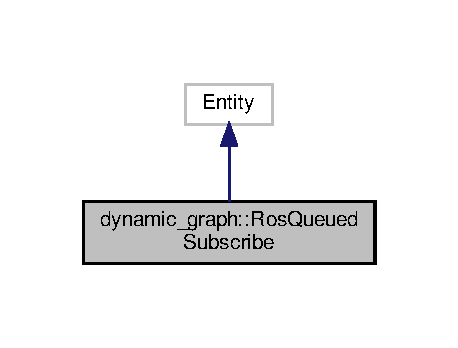
\includegraphics[width=220pt]{classdynamic__graph_1_1RosQueuedSubscribe__inherit__graph}
\end{center}
\end{figure}


Collaboration diagram for dynamic\+\_\+graph\+:\+:Ros\+Queued\+Subscribe\+:
\nopagebreak
\begin{figure}[H]
\begin{center}
\leavevmode
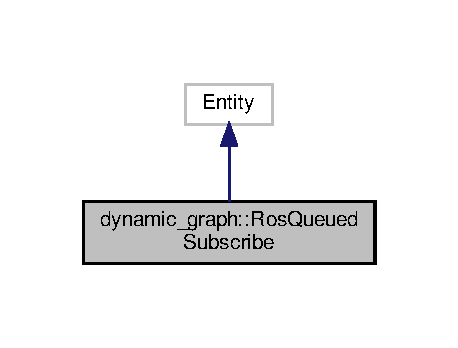
\includegraphics[width=220pt]{classdynamic__graph_1_1RosQueuedSubscribe__coll__graph}
\end{center}
\end{figure}
\subsection*{Public Types}
\begin{DoxyCompactItemize}
\item 
\mbox{\Hypertarget{classdynamic__graph_1_1RosQueuedSubscribe_a2f75c04157d429fa28dbce0e307762af}\label{classdynamic__graph_1_1RosQueuedSubscribe_a2f75c04157d429fa28dbce0e307762af}} 
typedef boost\+::shared\+\_\+ptr$<$ \hyperlink{structdynamic__graph_1_1internal_1_1BindedSignalBase}{internal\+::\+Binded\+Signal\+Base} $>$ {\bfseries binded\+Signal\+\_\+t}
\end{DoxyCompactItemize}
\subsection*{Public Member Functions}
\begin{DoxyCompactItemize}
\item 
\mbox{\Hypertarget{classdynamic__graph_1_1RosQueuedSubscribe_ad8a0a8fb42bbd51f47c810119c27693b}\label{classdynamic__graph_1_1RosQueuedSubscribe_ad8a0a8fb42bbd51f47c810119c27693b}} 
{\bfseries Ros\+Queued\+Subscribe} (const std\+::string \&n)
\item 
\mbox{\Hypertarget{classdynamic__graph_1_1RosQueuedSubscribe_ac145661ffbefb4979a471659cd6ee8cd}\label{classdynamic__graph_1_1RosQueuedSubscribe_ac145661ffbefb4979a471659cd6ee8cd}} 
virtual std\+::string {\bfseries get\+Doc\+String} () const
\item 
\mbox{\Hypertarget{classdynamic__graph_1_1RosQueuedSubscribe_af8941fff1c6cd450d84f7b2b2b26cee5}\label{classdynamic__graph_1_1RosQueuedSubscribe_af8941fff1c6cd450d84f7b2b2b26cee5}} 
void {\bfseries display} (std\+::ostream \&os) const
\item 
\mbox{\Hypertarget{classdynamic__graph_1_1RosQueuedSubscribe_a1bde97a76f12a84467c1ab4f5fd13ad0}\label{classdynamic__graph_1_1RosQueuedSubscribe_a1bde97a76f12a84467c1ab4f5fd13ad0}} 
void {\bfseries rm} (const std\+::string \&signal)
\item 
\mbox{\Hypertarget{classdynamic__graph_1_1RosQueuedSubscribe_a098c82686aa747d2bb6a0d1f2f9d4e3d}\label{classdynamic__graph_1_1RosQueuedSubscribe_a098c82686aa747d2bb6a0d1f2f9d4e3d}} 
std\+::string {\bfseries list} ()
\item 
\mbox{\Hypertarget{classdynamic__graph_1_1RosQueuedSubscribe_a5089fd7d1f253b80f292849f53352610}\label{classdynamic__graph_1_1RosQueuedSubscribe_a5089fd7d1f253b80f292849f53352610}} 
void {\bfseries clear} ()
\item 
\mbox{\Hypertarget{classdynamic__graph_1_1RosQueuedSubscribe_af8baae6f2b1ed8cf0f5d66118a2eb968}\label{classdynamic__graph_1_1RosQueuedSubscribe_af8baae6f2b1ed8cf0f5d66118a2eb968}} 
void {\bfseries clear\+Queue} (const std\+::string \&signal)
\item 
\mbox{\Hypertarget{classdynamic__graph_1_1RosQueuedSubscribe_ad93d84cc27a7bee9d2306d43246a3ecc}\label{classdynamic__graph_1_1RosQueuedSubscribe_ad93d84cc27a7bee9d2306d43246a3ecc}} 
void {\bfseries read\+Queue} (int begin\+Reading\+At)
\item 
\mbox{\Hypertarget{classdynamic__graph_1_1RosQueuedSubscribe_a1d1be7dd45b585d589c08930a06d5125}\label{classdynamic__graph_1_1RosQueuedSubscribe_a1d1be7dd45b585d589c08930a06d5125}} 
std\+::size\+\_\+t {\bfseries queue\+Size} (const std\+::string \&signal) const
\item 
\mbox{\Hypertarget{classdynamic__graph_1_1RosQueuedSubscribe_ad676b92e3c68923c36e0794df9a36b07}\label{classdynamic__graph_1_1RosQueuedSubscribe_ad676b92e3c68923c36e0794df9a36b07}} 
{\footnotesize template$<$typename T $>$ }\\void {\bfseries add} (const std\+::string \&type, const std\+::string \&signal, const std\+::string \&topic)
\item 
\mbox{\Hypertarget{classdynamic__graph_1_1RosQueuedSubscribe_ab6a37292689cb3798d9348561a2b6796}\label{classdynamic__graph_1_1RosQueuedSubscribe_ab6a37292689cb3798d9348561a2b6796}} 
std\+::map$<$ std\+::string, binded\+Signal\+\_\+t $>$ \& {\bfseries binded\+Signal} ()
\item 
\mbox{\Hypertarget{classdynamic__graph_1_1RosQueuedSubscribe_a2e5ddc40978683c8c5ee5e1a6758aa22}\label{classdynamic__graph_1_1RosQueuedSubscribe_a2e5ddc40978683c8c5ee5e1a6758aa22}} 
ros\+::\+Node\+Handle \& {\bfseries nh} ()
\item 
\mbox{\Hypertarget{classdynamic__graph_1_1RosQueuedSubscribe_afe57f995f66aa7bbf5d006e876cdbd66}\label{classdynamic__graph_1_1RosQueuedSubscribe_afe57f995f66aa7bbf5d006e876cdbd66}} 
{\footnotesize template$<$typename R , typename S $>$ }\\void {\bfseries callback} (boost\+::shared\+\_\+ptr$<$ dynamicgraph\+::\+Signal\+Ptr$<$ S, int $>$ $>$ signal, const R \&data)
\item 
\mbox{\Hypertarget{classdynamic__graph_1_1RosQueuedSubscribe_acfb7c66275aa4680cf0c6b40edeabb9d}\label{classdynamic__graph_1_1RosQueuedSubscribe_acfb7c66275aa4680cf0c6b40edeabb9d}} 
{\footnotesize template$<$typename R $>$ }\\void {\bfseries callback\+Timestamp} (boost\+::shared\+\_\+ptr$<$ dynamicgraph\+::\+Signal\+Ptr$<$ ptime, int $>$ $>$ signal, const R \&data)
\item 
\mbox{\Hypertarget{classdynamic__graph_1_1RosQueuedSubscribe_a274d716f1f8fdba71963dd04db0fefd4}\label{classdynamic__graph_1_1RosQueuedSubscribe_a274d716f1f8fdba71963dd04db0fefd4}} 
int {\bfseries read\+Queue} ()
\end{DoxyCompactItemize}
\subsection*{Private Types}
\begin{DoxyCompactItemize}
\item 
\mbox{\Hypertarget{classdynamic__graph_1_1RosQueuedSubscribe_a78091d9cf016f41283ca5a793b9cd486}\label{classdynamic__graph_1_1RosQueuedSubscribe_a78091d9cf016f41283ca5a793b9cd486}} 
typedef boost\+::posix\+\_\+time\+::ptime {\bfseries ptime}
\end{DoxyCompactItemize}
\subsection*{Private Member Functions}
\begin{DoxyCompactItemize}
\item 
\mbox{\Hypertarget{classdynamic__graph_1_1RosQueuedSubscribe_a3d52d1de001cc0b71410b3da7429a751}\label{classdynamic__graph_1_1RosQueuedSubscribe_a3d52d1de001cc0b71410b3da7429a751}} 
{\bfseries D\+Y\+N\+A\+M\+I\+C\+\_\+\+G\+R\+A\+P\+H\+\_\+\+E\+N\+T\+I\+T\+Y\+\_\+\+D\+E\+CL} ()
\end{DoxyCompactItemize}
\subsection*{Private Attributes}
\begin{DoxyCompactItemize}
\item 
\mbox{\Hypertarget{classdynamic__graph_1_1RosQueuedSubscribe_a4795502ea5dc4f01158b850cc3f63f00}\label{classdynamic__graph_1_1RosQueuedSubscribe_a4795502ea5dc4f01158b850cc3f63f00}} 
ros\+::\+Node\+Handle \& {\bfseries nh\+\_\+}
\item 
\mbox{\Hypertarget{classdynamic__graph_1_1RosQueuedSubscribe_acb4476833404b04da8012ed5a4c84150}\label{classdynamic__graph_1_1RosQueuedSubscribe_acb4476833404b04da8012ed5a4c84150}} 
std\+::map$<$ std\+::string, binded\+Signal\+\_\+t $>$ {\bfseries binded\+Signal\+\_\+}
\item 
\mbox{\Hypertarget{classdynamic__graph_1_1RosQueuedSubscribe_a264c8494a5545e63679ad0bfdb4dd614}\label{classdynamic__graph_1_1RosQueuedSubscribe_a264c8494a5545e63679ad0bfdb4dd614}} 
int {\bfseries read\+Queue\+\_\+}
\end{DoxyCompactItemize}
\subsection*{Static Private Attributes}
\begin{DoxyCompactItemize}
\item 
\mbox{\Hypertarget{classdynamic__graph_1_1RosQueuedSubscribe_a07f6aa0c68e2a97c04fce2b001c41f75}\label{classdynamic__graph_1_1RosQueuedSubscribe_a07f6aa0c68e2a97c04fce2b001c41f75}} 
static const std\+::string {\bfseries docstring\+\_\+}
\end{DoxyCompactItemize}
\subsection*{Friends}
\begin{DoxyCompactItemize}
\item 
\mbox{\Hypertarget{classdynamic__graph_1_1RosQueuedSubscribe_aff86e359edc93019ec7be05f8207a40d}\label{classdynamic__graph_1_1RosQueuedSubscribe_aff86e359edc93019ec7be05f8207a40d}} 
{\footnotesize template$<$typename T $>$ }\\class {\bfseries internal\+::\+Add}
\item 
\mbox{\Hypertarget{classdynamic__graph_1_1RosQueuedSubscribe_a9df2fc52f650be6e579db5873effd4e8}\label{classdynamic__graph_1_1RosQueuedSubscribe_a9df2fc52f650be6e579db5873effd4e8}} 
{\footnotesize template$<$typename T , int Buffer\+Size$>$ }\\class {\bfseries internal\+::\+Binded\+Signal}
\end{DoxyCompactItemize}


\subsection{Detailed Description}
Publish R\+OS information in the dynamic-\/graph. 

The documentation for this class was generated from the following files\+:\begin{DoxyCompactItemize}
\item 
include/ros\+\_\+entities/\hyperlink{ros__queued__subscribe_8hh}{ros\+\_\+queued\+\_\+subscribe.\+hh}\item 
include/ros\+\_\+entities/\hyperlink{ros__queued__subscribe_8hxx}{ros\+\_\+queued\+\_\+subscribe.\+hxx}\item 
src/ros\+\_\+entities/\hyperlink{ros__queued__subscribe_8cpp}{ros\+\_\+queued\+\_\+subscribe.\+cpp}\end{DoxyCompactItemize}

\hypertarget{classdynamic__graph_1_1RosRobotStatePublisher}{}\section{dynamic\+\_\+graph\+:\+:Ros\+Robot\+State\+Publisher Class Reference}
\label{classdynamic__graph_1_1RosRobotStatePublisher}\index{dynamic\+\_\+graph\+::\+Ros\+Robot\+State\+Publisher@{dynamic\+\_\+graph\+::\+Ros\+Robot\+State\+Publisher}}


This class define a dynamic graph wrapper around the vicon client.  




{\ttfamily \#include $<$ros\+\_\+robot\+\_\+state\+\_\+publisher.\+hpp$>$}



Inheritance diagram for dynamic\+\_\+graph\+:\+:Ros\+Robot\+State\+Publisher\+:
\nopagebreak
\begin{figure}[H]
\begin{center}
\leavevmode
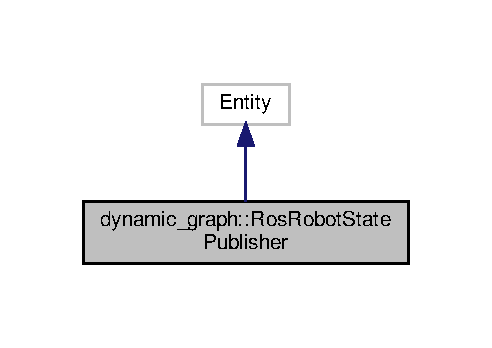
\includegraphics[width=236pt]{classdynamic__graph_1_1RosRobotStatePublisher__inherit__graph}
\end{center}
\end{figure}


Collaboration diagram for dynamic\+\_\+graph\+:\+:Ros\+Robot\+State\+Publisher\+:
\nopagebreak
\begin{figure}[H]
\begin{center}
\leavevmode
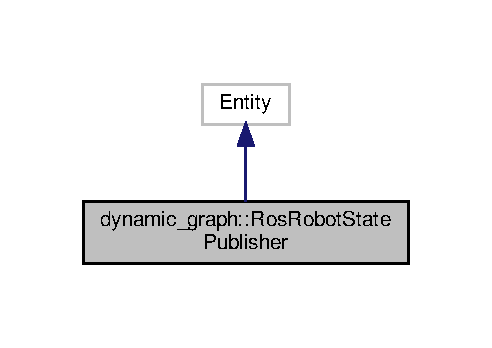
\includegraphics[width=236pt]{classdynamic__graph_1_1RosRobotStatePublisher__coll__graph}
\end{center}
\end{figure}
\subsection*{Public Member Functions}
\begin{DoxyCompactItemize}
\item 
\mbox{\Hypertarget{classdynamic__graph_1_1RosRobotStatePublisher_a7dbda339acfbacd6c2f45e7aac4409be}\label{classdynamic__graph_1_1RosRobotStatePublisher_a7dbda339acfbacd6c2f45e7aac4409be}} 
{\bfseries Ros\+Robot\+State\+Publisher} (const std\+::string \&name)
\item 
void \hyperlink{classdynamic__graph_1_1RosRobotStatePublisher_a92094934e53306e73b6fc13d1de61b3d}{add} (const std\+::string \&base\+\_\+link\+\_\+name, const std\+::string \&joint\+\_\+names, const std\+::string \&tf\+\_\+prefix, const std\+::string \&signal\+\_\+name, const std\+::string \&joint\+\_\+state\+\_\+topic\+\_\+name)
\item 
int \& \hyperlink{classdynamic__graph_1_1RosRobotStatePublisher_a4d66defbd1b308cd06394107f55f6cbb}{trigger} (int \&, int)
\begin{DoxyCompactList}\small\item\em Trigger the publishing of the data to ros for all signals. \end{DoxyCompactList}\item 
\mbox{\Hypertarget{classdynamic__graph_1_1RosRobotStatePublisher_a196621509ce1e5becada60a7093bcb3a}\label{classdynamic__graph_1_1RosRobotStatePublisher_a196621509ce1e5becada60a7093bcb3a}} 
void \hyperlink{classdynamic__graph_1_1RosRobotStatePublisher_a196621509ce1e5becada60a7093bcb3a}{send\+\_\+data} (const \hyperlink{structdynamic__graph_1_1RosRobotStatePublisherInternal}{Ros\+Robot\+State\+Publisher\+Internal} \&publisher, int time)
\begin{DoxyCompactList}\small\item\em Signal callback functions. \end{DoxyCompactList}\end{DoxyCompactItemize}
\subsection*{Private Member Functions}
\begin{DoxyCompactItemize}
\item 
virtual const std\+::string \& \hyperlink{classdynamic__graph_1_1RosRobotStatePublisher_aa031a669a2c2784c50b558fd2e2b6da3}{get\+Class\+Name} (void) const
\begin{DoxyCompactList}\small\item\em Get the C\+L\+A\+S\+S\+\_\+\+N\+A\+ME object. \end{DoxyCompactList}\item 
void \hyperlink{classdynamic__graph_1_1RosRobotStatePublisher_af3e0cfe13273ecd8c6e01b59bb6220e7}{set\+\_\+tf\+\_\+msg\+\_\+to\+\_\+identity} (geometry\+\_\+msgs\+::\+Transform\+Stamped \&msg)
\begin{DoxyCompactList}\small\item\em Set a tf msg to identity. \end{DoxyCompactList}\item 
void \hyperlink{classdynamic__graph_1_1RosRobotStatePublisher_acb4e771801c5bc13c7a2b022c3dd6b9d}{normalize\+\_\+tf\+\_\+msg\+\_\+quaternion} (geometry\+\_\+msgs\+::\+Transform\+Stamped \&msg)
\begin{DoxyCompactList}\small\item\em Normalize the tf message quaternion before sending it to the. \end{DoxyCompactList}\end{DoxyCompactItemize}
\subsection*{Private Attributes}
\begin{DoxyCompactItemize}
\item 
\hyperlink{namespacedynamic__graph_a9d80c350c95e161319d7a6e629ecdc4b}{Signal\+O\+UT} \hyperlink{classdynamic__graph_1_1RosRobotStatePublisher_a175914c0624474d019cb1360fa9c14e4}{trigger\+\_\+signal\+\_\+}
\begin{DoxyCompactList}\small\item\em Create an internal output signal which should be call periodically in the device in order to publish the data. \end{DoxyCompactList}\item 
\mbox{\Hypertarget{classdynamic__graph_1_1RosRobotStatePublisher_a5b494e473d93118cb69320c01dfd772c}\label{classdynamic__graph_1_1RosRobotStatePublisher_a5b494e473d93118cb69320c01dfd772c}} 
ros\+::\+Node\+Handle \& \hyperlink{classdynamic__graph_1_1RosRobotStatePublisher_a5b494e473d93118cb69320c01dfd772c}{ros\+\_\+node\+\_\+handle\+\_\+}
\begin{DoxyCompactList}\small\item\em Ros node handle corresponding to the dynamic graph process node handle. \end{DoxyCompactList}\item 
std\+::map$<$ std\+::string, \hyperlink{structdynamic__graph_1_1RosRobotStatePublisherInternal}{Ros\+Robot\+State\+Publisher\+Internal} $>$ \hyperlink{classdynamic__graph_1_1RosRobotStatePublisher_a556fe3ed8d7c0786e0d6aad4cbb415db}{publishers\+\_\+}
\begin{DoxyCompactList}\small\item\em This is the list of publishers registered for this class. \end{DoxyCompactList}\item 
\mbox{\Hypertarget{classdynamic__graph_1_1RosRobotStatePublisher_af638eb336998964161a89e4ce76821d1}\label{classdynamic__graph_1_1RosRobotStatePublisher_af638eb336998964161a89e4ce76821d1}} 
ros\+::\+Duration \hyperlink{classdynamic__graph_1_1RosRobotStatePublisher_af638eb336998964161a89e4ce76821d1}{rate\+\_\+}
\begin{DoxyCompactList}\small\item\em manage the rate data publication in topics \end{DoxyCompactList}\item 
\mbox{\Hypertarget{classdynamic__graph_1_1RosRobotStatePublisher_a000e917f448ac480bfc8b2559d41a4b5}\label{classdynamic__graph_1_1RosRobotStatePublisher_a000e917f448ac480bfc8b2559d41a4b5}} 
ros\+::\+Time \hyperlink{classdynamic__graph_1_1RosRobotStatePublisher_a000e917f448ac480bfc8b2559d41a4b5}{last\+\_\+time\+\_\+of\+\_\+publication\+\_\+}
\begin{DoxyCompactList}\small\item\em Check at what time the publication was done. \end{DoxyCompactList}\end{DoxyCompactItemize}
\subsection*{Static Private Attributes}
\begin{DoxyCompactItemize}
\item 
\mbox{\Hypertarget{classdynamic__graph_1_1RosRobotStatePublisher_a3794be6383ba4bc9a7412218a755f524}\label{classdynamic__graph_1_1RosRobotStatePublisher_a3794be6383ba4bc9a7412218a755f524}} 
static const std\+::string \hyperlink{classdynamic__graph_1_1RosRobotStatePublisher_a3794be6383ba4bc9a7412218a755f524}{C\+L\+A\+S\+S\+\_\+\+N\+A\+ME}
\begin{DoxyCompactList}\small\item\em The class name used to identify it in the dynamic graph pool. \end{DoxyCompactList}\end{DoxyCompactItemize}


\subsection{Detailed Description}
This class define a dynamic graph wrapper around the vicon client. 

\subsection{Member Function Documentation}
\mbox{\Hypertarget{classdynamic__graph_1_1RosRobotStatePublisher_a92094934e53306e73b6fc13d1de61b3d}\label{classdynamic__graph_1_1RosRobotStatePublisher_a92094934e53306e73b6fc13d1de61b3d}} 
\index{dynamic\+\_\+graph\+::\+Ros\+Robot\+State\+Publisher@{dynamic\+\_\+graph\+::\+Ros\+Robot\+State\+Publisher}!add@{add}}
\index{add@{add}!dynamic\+\_\+graph\+::\+Ros\+Robot\+State\+Publisher@{dynamic\+\_\+graph\+::\+Ros\+Robot\+State\+Publisher}}
\subsubsection{\texorpdfstring{add()}{add()}}
{\footnotesize\ttfamily void dynamic\+\_\+graph\+::\+Ros\+Robot\+State\+Publisher\+::add (\begin{DoxyParamCaption}\item[{const std\+::string \&}]{base\+\_\+link\+\_\+name,  }\item[{const std\+::string \&}]{joint\+\_\+names,  }\item[{const std\+::string \&}]{tf\+\_\+prefix,  }\item[{const std\+::string \&}]{signal\+\_\+name,  }\item[{const std\+::string \&}]{joint\+\_\+state\+\_\+topic\+\_\+name }\end{DoxyParamCaption})}


\begin{DoxyParams}{Parameters}
{\em base\+\_\+link\+\_\+name} & \\
\hline
{\em joint\+\_\+names} & \\
\hline
{\em tf\+\_\+prefix} & \\
\hline
{\em signal\+\_\+name} & \\
\hline
\end{DoxyParams}
\mbox{\Hypertarget{classdynamic__graph_1_1RosRobotStatePublisher_aa031a669a2c2784c50b558fd2e2b6da3}\label{classdynamic__graph_1_1RosRobotStatePublisher_aa031a669a2c2784c50b558fd2e2b6da3}} 
\index{dynamic\+\_\+graph\+::\+Ros\+Robot\+State\+Publisher@{dynamic\+\_\+graph\+::\+Ros\+Robot\+State\+Publisher}!get\+Class\+Name@{get\+Class\+Name}}
\index{get\+Class\+Name@{get\+Class\+Name}!dynamic\+\_\+graph\+::\+Ros\+Robot\+State\+Publisher@{dynamic\+\_\+graph\+::\+Ros\+Robot\+State\+Publisher}}
\subsubsection{\texorpdfstring{get\+Class\+Name()}{getClassName()}}
{\footnotesize\ttfamily virtual const std\+::string\& dynamic\+\_\+graph\+::\+Ros\+Robot\+State\+Publisher\+::get\+Class\+Name (\begin{DoxyParamCaption}\item[{void}]{ }\end{DoxyParamCaption}) const\hspace{0.3cm}{\ttfamily [inline]}, {\ttfamily [private]}, {\ttfamily [virtual]}}



Get the C\+L\+A\+S\+S\+\_\+\+N\+A\+ME object. 

\begin{DoxyReturn}{Returns}
const std\+::string\& 
\end{DoxyReturn}
\mbox{\Hypertarget{classdynamic__graph_1_1RosRobotStatePublisher_acb4e771801c5bc13c7a2b022c3dd6b9d}\label{classdynamic__graph_1_1RosRobotStatePublisher_acb4e771801c5bc13c7a2b022c3dd6b9d}} 
\index{dynamic\+\_\+graph\+::\+Ros\+Robot\+State\+Publisher@{dynamic\+\_\+graph\+::\+Ros\+Robot\+State\+Publisher}!normalize\+\_\+tf\+\_\+msg\+\_\+quaternion@{normalize\+\_\+tf\+\_\+msg\+\_\+quaternion}}
\index{normalize\+\_\+tf\+\_\+msg\+\_\+quaternion@{normalize\+\_\+tf\+\_\+msg\+\_\+quaternion}!dynamic\+\_\+graph\+::\+Ros\+Robot\+State\+Publisher@{dynamic\+\_\+graph\+::\+Ros\+Robot\+State\+Publisher}}
\subsubsection{\texorpdfstring{normalize\+\_\+tf\+\_\+msg\+\_\+quaternion()}{normalize\_tf\_msg\_quaternion()}}
{\footnotesize\ttfamily void dynamic\+\_\+graph\+::\+Ros\+Robot\+State\+Publisher\+::normalize\+\_\+tf\+\_\+msg\+\_\+quaternion (\begin{DoxyParamCaption}\item[{geometry\+\_\+msgs\+::\+Transform\+Stamped \&}]{msg }\end{DoxyParamCaption})\hspace{0.3cm}{\ttfamily [private]}}



Normalize the tf message quaternion before sending it to the. 


\begin{DoxyParams}[1]{Parameters}
\mbox{\tt in}  & {\em } & \\
\hline
\end{DoxyParams}
\mbox{\Hypertarget{classdynamic__graph_1_1RosRobotStatePublisher_af3e0cfe13273ecd8c6e01b59bb6220e7}\label{classdynamic__graph_1_1RosRobotStatePublisher_af3e0cfe13273ecd8c6e01b59bb6220e7}} 
\index{dynamic\+\_\+graph\+::\+Ros\+Robot\+State\+Publisher@{dynamic\+\_\+graph\+::\+Ros\+Robot\+State\+Publisher}!set\+\_\+tf\+\_\+msg\+\_\+to\+\_\+identity@{set\+\_\+tf\+\_\+msg\+\_\+to\+\_\+identity}}
\index{set\+\_\+tf\+\_\+msg\+\_\+to\+\_\+identity@{set\+\_\+tf\+\_\+msg\+\_\+to\+\_\+identity}!dynamic\+\_\+graph\+::\+Ros\+Robot\+State\+Publisher@{dynamic\+\_\+graph\+::\+Ros\+Robot\+State\+Publisher}}
\subsubsection{\texorpdfstring{set\+\_\+tf\+\_\+msg\+\_\+to\+\_\+identity()}{set\_tf\_msg\_to\_identity()}}
{\footnotesize\ttfamily void dynamic\+\_\+graph\+::\+Ros\+Robot\+State\+Publisher\+::set\+\_\+tf\+\_\+msg\+\_\+to\+\_\+identity (\begin{DoxyParamCaption}\item[{geometry\+\_\+msgs\+::\+Transform\+Stamped \&}]{msg }\end{DoxyParamCaption})\hspace{0.3cm}{\ttfamily [private]}}



Set a tf msg to identity. 


\begin{DoxyParams}[1]{Parameters}
\mbox{\tt in}  & {\em } & \\
\hline
\end{DoxyParams}
\mbox{\Hypertarget{classdynamic__graph_1_1RosRobotStatePublisher_a4d66defbd1b308cd06394107f55f6cbb}\label{classdynamic__graph_1_1RosRobotStatePublisher_a4d66defbd1b308cd06394107f55f6cbb}} 
\index{dynamic\+\_\+graph\+::\+Ros\+Robot\+State\+Publisher@{dynamic\+\_\+graph\+::\+Ros\+Robot\+State\+Publisher}!trigger@{trigger}}
\index{trigger@{trigger}!dynamic\+\_\+graph\+::\+Ros\+Robot\+State\+Publisher@{dynamic\+\_\+graph\+::\+Ros\+Robot\+State\+Publisher}}
\subsubsection{\texorpdfstring{trigger()}{trigger()}}
{\footnotesize\ttfamily int \& dynamic\+\_\+graph\+::\+Ros\+Robot\+State\+Publisher\+::trigger (\begin{DoxyParamCaption}\item[{int \&}]{dummy,  }\item[{int}]{time }\end{DoxyParamCaption})}



Trigger the publishing of the data to ros for all signals. 

\begin{DoxyReturn}{Returns}
int\& dummy stuff. 
\end{DoxyReturn}


\subsection{Member Data Documentation}
\mbox{\Hypertarget{classdynamic__graph_1_1RosRobotStatePublisher_a556fe3ed8d7c0786e0d6aad4cbb415db}\label{classdynamic__graph_1_1RosRobotStatePublisher_a556fe3ed8d7c0786e0d6aad4cbb415db}} 
\index{dynamic\+\_\+graph\+::\+Ros\+Robot\+State\+Publisher@{dynamic\+\_\+graph\+::\+Ros\+Robot\+State\+Publisher}!publishers\+\_\+@{publishers\+\_\+}}
\index{publishers\+\_\+@{publishers\+\_\+}!dynamic\+\_\+graph\+::\+Ros\+Robot\+State\+Publisher@{dynamic\+\_\+graph\+::\+Ros\+Robot\+State\+Publisher}}
\subsubsection{\texorpdfstring{publishers\+\_\+}{publishers\_}}
{\footnotesize\ttfamily std\+::map$<$std\+::string, \hyperlink{structdynamic__graph_1_1RosRobotStatePublisherInternal}{Ros\+Robot\+State\+Publisher\+Internal}$>$ dynamic\+\_\+graph\+::\+Ros\+Robot\+State\+Publisher\+::publishers\+\_\+\hspace{0.3cm}{\ttfamily [private]}}



This is the list of publishers registered for this class. 

It correspond to the list of robot states one wants to publish. See the add methode (Command) \mbox{\Hypertarget{classdynamic__graph_1_1RosRobotStatePublisher_a175914c0624474d019cb1360fa9c14e4}\label{classdynamic__graph_1_1RosRobotStatePublisher_a175914c0624474d019cb1360fa9c14e4}} 
\index{dynamic\+\_\+graph\+::\+Ros\+Robot\+State\+Publisher@{dynamic\+\_\+graph\+::\+Ros\+Robot\+State\+Publisher}!trigger\+\_\+signal\+\_\+@{trigger\+\_\+signal\+\_\+}}
\index{trigger\+\_\+signal\+\_\+@{trigger\+\_\+signal\+\_\+}!dynamic\+\_\+graph\+::\+Ros\+Robot\+State\+Publisher@{dynamic\+\_\+graph\+::\+Ros\+Robot\+State\+Publisher}}
\subsubsection{\texorpdfstring{trigger\+\_\+signal\+\_\+}{trigger\_signal\_}}
{\footnotesize\ttfamily \hyperlink{namespacedynamic__graph_a9d80c350c95e161319d7a6e629ecdc4b}{Signal\+O\+UT} dynamic\+\_\+graph\+::\+Ros\+Robot\+State\+Publisher\+::trigger\+\_\+signal\+\_\+\hspace{0.3cm}{\ttfamily [private]}}



Create an internal output signal which should be call periodically in the device in order to publish the data. 

The callback function of this signal is the trigger methode. 

The documentation for this class was generated from the following files\+:\begin{DoxyCompactItemize}
\item 
include/ros\+\_\+entities/\hyperlink{ros__robot__state__publisher_8hpp}{ros\+\_\+robot\+\_\+state\+\_\+publisher.\+hpp}\item 
src/ros\+\_\+entities/\hyperlink{ros__robot__state__publisher_8cpp}{ros\+\_\+robot\+\_\+state\+\_\+publisher.\+cpp}\end{DoxyCompactItemize}

\hypertarget{structdynamic__graph_1_1RosRobotStatePublisherInternal}{}\section{dynamic\+\_\+graph\+:\+:Ros\+Robot\+State\+Publisher\+Internal Struct Reference}
\label{structdynamic__graph_1_1RosRobotStatePublisherInternal}\index{dynamic\+\_\+graph\+::\+Ros\+Robot\+State\+Publisher\+Internal@{dynamic\+\_\+graph\+::\+Ros\+Robot\+State\+Publisher\+Internal}}
\subsection*{Public Attributes}
\begin{DoxyCompactItemize}
\item 
std\+::shared\+\_\+ptr$<$ \hyperlink{namespacedynamic__graph_ac8d567b9a3d1ab846ba2efdc1ff1e120}{Tf\+Rt\+Publisher} $>$ {\bfseries base\+\_\+tf\+\_\+publisher\+\_\+}\hypertarget{structdynamic__graph_1_1RosRobotStatePublisherInternal_a99b630f10c0d338da1da2945f7c7f906}{}\label{structdynamic__graph_1_1RosRobotStatePublisherInternal_a99b630f10c0d338da1da2945f7c7f906}

\item 
std\+::shared\+\_\+ptr$<$ \hyperlink{namespacedynamic__graph_ae9ad83c8174a9aa5bc1688df02b4ee95}{Joint\+State\+Rt\+Publisher} $>$ {\bfseries joint\+\_\+state\+\_\+publisher\+\_\+}\hypertarget{structdynamic__graph_1_1RosRobotStatePublisherInternal_ac04f31a05e4c55eb8f28351af8f9cbf6}{}\label{structdynamic__graph_1_1RosRobotStatePublisherInternal_ac04f31a05e4c55eb8f28351af8f9cbf6}

\item 
std\+::shared\+\_\+ptr$<$ \hyperlink{namespacedynamic__graph_ae1463c695a6915ea3f9ab4311beb527a}{Signal\+IN} $>$ {\bfseries robot\+\_\+state\+\_\+input\+\_\+signal\+\_\+}\hypertarget{structdynamic__graph_1_1RosRobotStatePublisherInternal_aacbcfcb6f326e672f555468111af7d56}{}\label{structdynamic__graph_1_1RosRobotStatePublisherInternal_aacbcfcb6f326e672f555468111af7d56}

\item 
\hyperlink{namespacedynamic__graph_adf7d40f2a8d1425af80c14f90e58e961}{callback\+\_\+t} {\bfseries callback\+\_\+function\+\_\+}\hypertarget{structdynamic__graph_1_1RosRobotStatePublisherInternal_a2aa4d44e955ec44e762deb1059b3e3f7}{}\label{structdynamic__graph_1_1RosRobotStatePublisherInternal_a2aa4d44e955ec44e762deb1059b3e3f7}

\end{DoxyCompactItemize}


The documentation for this struct was generated from the following file\+:\begin{DoxyCompactItemize}
\item 
include/ros\+\_\+entities/\hyperlink{ros__robot__state__publisher_8hpp}{ros\+\_\+robot\+\_\+state\+\_\+publisher.\+hpp}\end{DoxyCompactItemize}

\hypertarget{classdynamic__graph_1_1RosRobotStatePublisherMt}{}\section{dynamic\+\_\+graph\+:\+:Ros\+Robot\+State\+Publisher\+Mt Class Reference}
\label{classdynamic__graph_1_1RosRobotStatePublisherMt}\index{dynamic\+\_\+graph\+::\+Ros\+Robot\+State\+Publisher\+Mt@{dynamic\+\_\+graph\+::\+Ros\+Robot\+State\+Publisher\+Mt}}


This class define a dynamic graph wrapper around the vicon client.  




{\ttfamily \#include $<$ros\+\_\+robot\+\_\+state\+\_\+publisher\+\_\+mt.\+hpp$>$}



Inheritance diagram for dynamic\+\_\+graph\+:\+:Ros\+Robot\+State\+Publisher\+Mt\+:\nopagebreak
\begin{figure}[H]
\begin{center}
\leavevmode
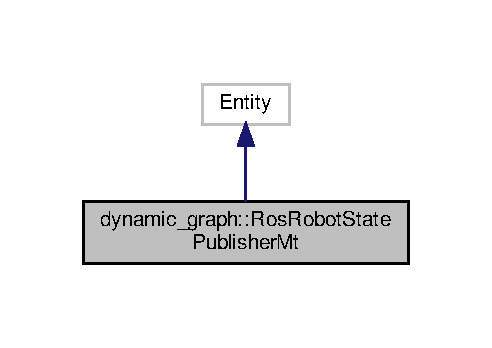
\includegraphics[width=236pt]{classdynamic__graph_1_1RosRobotStatePublisherMt__inherit__graph}
\end{center}
\end{figure}


Collaboration diagram for dynamic\+\_\+graph\+:\+:Ros\+Robot\+State\+Publisher\+Mt\+:\nopagebreak
\begin{figure}[H]
\begin{center}
\leavevmode
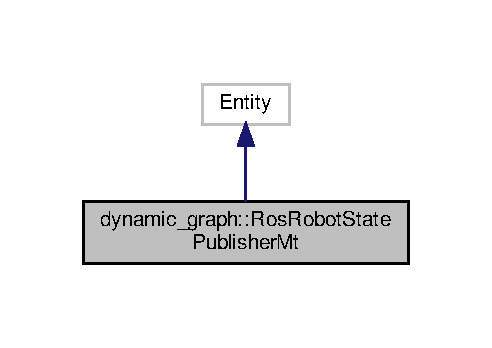
\includegraphics[width=236pt]{classdynamic__graph_1_1RosRobotStatePublisherMt__coll__graph}
\end{center}
\end{figure}
\subsection*{Public Member Functions}
\begin{DoxyCompactItemize}
\item 
{\bfseries Ros\+Robot\+State\+Publisher\+Mt} (const std\+::string \&name)\hypertarget{classdynamic__graph_1_1RosRobotStatePublisherMt_a26e240ba4685f64c462a25d783d454e1}{}\label{classdynamic__graph_1_1RosRobotStatePublisherMt_a26e240ba4685f64c462a25d783d454e1}

\item 
void \hyperlink{classdynamic__graph_1_1RosRobotStatePublisherMt_a2a3280fbd7d9f71c76481830ad71593c}{add} (const std\+::string \&base\+\_\+link\+\_\+name, const std\+::string \&joint\+\_\+names, const std\+::string \&tf\+\_\+prefix, const std\+::string \&signal\+\_\+name, const std\+::string \&joint\+\_\+state\+\_\+topic\+\_\+name)
\item 
int \& \hyperlink{classdynamic__graph_1_1RosRobotStatePublisherMt_ab246d4672cb6ccf5d0733dae31c5adbf}{trigger} (int \&, int)
\begin{DoxyCompactList}\small\item\em Trigger the publishing of the data to ros for all signals. \end{DoxyCompactList}\item 
void \hyperlink{classdynamic__graph_1_1RosRobotStatePublisherMt_a80a4f8a4d9cf9be7c40927ae05d1897f}{copy\+\_\+data\+\_\+internally} (std\+::shared\+\_\+ptr$<$ \hyperlink{structdynamic__graph_1_1RosRobotStatePublisherMtInternal}{Ros\+Robot\+State\+Publisher\+Mt\+Internal} $>$ publisher, int dg\+\_\+time)
\begin{DoxyCompactList}\small\item\em Signal callback functions. \end{DoxyCompactList}\item 
void \hyperlink{classdynamic__graph_1_1RosRobotStatePublisherMt_ac1826cd456058c929f709b3684d85544}{send\+\_\+data} (\hyperlink{structdynamic__graph_1_1RosRobotStatePublisherMtInternal}{Ros\+Robot\+State\+Publisher\+Mt\+Internal} \&publisher)\hypertarget{classdynamic__graph_1_1RosRobotStatePublisherMt_ac1826cd456058c929f709b3684d85544}{}\label{classdynamic__graph_1_1RosRobotStatePublisherMt_ac1826cd456058c929f709b3684d85544}

\begin{DoxyCompactList}\small\item\em Signal callback functions. \end{DoxyCompactList}\end{DoxyCompactItemize}


\subsection{Detailed Description}
This class define a dynamic graph wrapper around the vicon client. 

\subsection{Member Function Documentation}
\index{dynamic\+\_\+graph\+::\+Ros\+Robot\+State\+Publisher\+Mt@{dynamic\+\_\+graph\+::\+Ros\+Robot\+State\+Publisher\+Mt}!add@{add}}
\index{add@{add}!dynamic\+\_\+graph\+::\+Ros\+Robot\+State\+Publisher\+Mt@{dynamic\+\_\+graph\+::\+Ros\+Robot\+State\+Publisher\+Mt}}
\subsubsection[{\texorpdfstring{add(const std\+::string \&base\+\_\+link\+\_\+name, const std\+::string \&joint\+\_\+names, const std\+::string \&tf\+\_\+prefix, const std\+::string \&signal\+\_\+name, const std\+::string \&joint\+\_\+state\+\_\+topic\+\_\+name)}{add(const std::string &base_link_name, const std::string &joint_names, const std::string &tf_prefix, const std::string &signal_name, const std::string &joint_state_topic_name)}}]{\setlength{\rightskip}{0pt plus 5cm}void dynamic\+\_\+graph\+::\+Ros\+Robot\+State\+Publisher\+Mt\+::add (
\begin{DoxyParamCaption}
\item[{const std\+::string \&}]{base\+\_\+link\+\_\+name, }
\item[{const std\+::string \&}]{joint\+\_\+names, }
\item[{const std\+::string \&}]{tf\+\_\+prefix, }
\item[{const std\+::string \&}]{signal\+\_\+name, }
\item[{const std\+::string \&}]{joint\+\_\+state\+\_\+topic\+\_\+name}
\end{DoxyParamCaption}
)}\hypertarget{classdynamic__graph_1_1RosRobotStatePublisherMt_a2a3280fbd7d9f71c76481830ad71593c}{}\label{classdynamic__graph_1_1RosRobotStatePublisherMt_a2a3280fbd7d9f71c76481830ad71593c}

\begin{DoxyParams}{Parameters}
{\em base\+\_\+link\+\_\+name} & \\
\hline
{\em joint\+\_\+names} & \\
\hline
{\em tf\+\_\+prefix} & \\
\hline
{\em signal\+\_\+name} & \\
\hline
\end{DoxyParams}
\index{dynamic\+\_\+graph\+::\+Ros\+Robot\+State\+Publisher\+Mt@{dynamic\+\_\+graph\+::\+Ros\+Robot\+State\+Publisher\+Mt}!copy\+\_\+data\+\_\+internally@{copy\+\_\+data\+\_\+internally}}
\index{copy\+\_\+data\+\_\+internally@{copy\+\_\+data\+\_\+internally}!dynamic\+\_\+graph\+::\+Ros\+Robot\+State\+Publisher\+Mt@{dynamic\+\_\+graph\+::\+Ros\+Robot\+State\+Publisher\+Mt}}
\subsubsection[{\texorpdfstring{copy\+\_\+data\+\_\+internally(std\+::shared\+\_\+ptr$<$ Ros\+Robot\+State\+Publisher\+Mt\+Internal $>$ publisher, int dg\+\_\+time)}{copy_data_internally(std::shared_ptr< RosRobotStatePublisherMtInternal > publisher, int dg_time)}}]{\setlength{\rightskip}{0pt plus 5cm}void dynamic\+\_\+graph\+::\+Ros\+Robot\+State\+Publisher\+Mt\+::copy\+\_\+data\+\_\+internally (
\begin{DoxyParamCaption}
\item[{std\+::shared\+\_\+ptr$<$ {\bf Ros\+Robot\+State\+Publisher\+Mt\+Internal} $>$}]{publisher, }
\item[{int}]{dg\+\_\+time}
\end{DoxyParamCaption}
)}\hypertarget{classdynamic__graph_1_1RosRobotStatePublisherMt_a80a4f8a4d9cf9be7c40927ae05d1897f}{}\label{classdynamic__graph_1_1RosRobotStatePublisherMt_a80a4f8a4d9cf9be7c40927ae05d1897f}


Signal callback functions. 


\begin{DoxyParams}{Parameters}
{\em publisher} & is the ros real time publisher object. \\
\hline
{\em time} & the current signal time \\
\hline
\end{DoxyParams}
\index{dynamic\+\_\+graph\+::\+Ros\+Robot\+State\+Publisher\+Mt@{dynamic\+\_\+graph\+::\+Ros\+Robot\+State\+Publisher\+Mt}!trigger@{trigger}}
\index{trigger@{trigger}!dynamic\+\_\+graph\+::\+Ros\+Robot\+State\+Publisher\+Mt@{dynamic\+\_\+graph\+::\+Ros\+Robot\+State\+Publisher\+Mt}}
\subsubsection[{\texorpdfstring{trigger(int \&, int)}{trigger(int &, int)}}]{\setlength{\rightskip}{0pt plus 5cm}int \& dynamic\+\_\+graph\+::\+Ros\+Robot\+State\+Publisher\+Mt\+::trigger (
\begin{DoxyParamCaption}
\item[{int \&}]{dummy, }
\item[{int}]{dg\+\_\+time}
\end{DoxyParamCaption}
)}\hypertarget{classdynamic__graph_1_1RosRobotStatePublisherMt_ab246d4672cb6ccf5d0733dae31c5adbf}{}\label{classdynamic__graph_1_1RosRobotStatePublisherMt_ab246d4672cb6ccf5d0733dae31c5adbf}


Trigger the publishing of the data to ros for all signals. 

\begin{DoxyReturn}{Returns}
int\& dummy stuff. 
\end{DoxyReturn}


The documentation for this class was generated from the following files\+:\begin{DoxyCompactItemize}
\item 
/home/mnaveau/devel/workspace/src/catkin/dg\+\_\+control/dynamic\+\_\+graph\+\_\+manager/include/ros\+\_\+entities/\hyperlink{ros__robot__state__publisher__mt_8hpp}{ros\+\_\+robot\+\_\+state\+\_\+publisher\+\_\+mt.\+hpp}\item 
/home/mnaveau/devel/workspace/src/catkin/dg\+\_\+control/dynamic\+\_\+graph\+\_\+manager/src/ros\+\_\+entities/\hyperlink{ros__robot__state__publisher__mt_8cpp}{ros\+\_\+robot\+\_\+state\+\_\+publisher\+\_\+mt.\+cpp}\end{DoxyCompactItemize}

\hypertarget{structdynamic__graph_1_1RosRobotStatePublisherMtInternal}{}\section{dynamic\+\_\+graph\+:\+:Ros\+Robot\+State\+Publisher\+Mt\+Internal Struct Reference}
\label{structdynamic__graph_1_1RosRobotStatePublisherMtInternal}\index{dynamic\+\_\+graph\+::\+Ros\+Robot\+State\+Publisher\+Mt\+Internal@{dynamic\+\_\+graph\+::\+Ros\+Robot\+State\+Publisher\+Mt\+Internal}}
\subsection*{Public Attributes}
\begin{DoxyCompactItemize}
\item 
std\+::shared\+\_\+ptr$<$ \hyperlink{namespacedynamic__graph_ac8d567b9a3d1ab846ba2efdc1ff1e120}{Tf\+Rt\+Publisher} $>$ {\bfseries base\+\_\+tf\+\_\+publisher\+\_\+}\hypertarget{structdynamic__graph_1_1RosRobotStatePublisherMtInternal_aab90866aadd382e54d32f7fef36a2104}{}\label{structdynamic__graph_1_1RosRobotStatePublisherMtInternal_aab90866aadd382e54d32f7fef36a2104}

\item 
std\+::shared\+\_\+ptr$<$ \hyperlink{namespacedynamic__graph_ae9ad83c8174a9aa5bc1688df02b4ee95}{Joint\+State\+Rt\+Publisher} $>$ {\bfseries joint\+\_\+state\+\_\+publisher\+\_\+}\hypertarget{structdynamic__graph_1_1RosRobotStatePublisherMtInternal_a3d4474426dd6e6b7be683e0f3e9bbe93}{}\label{structdynamic__graph_1_1RosRobotStatePublisherMtInternal_a3d4474426dd6e6b7be683e0f3e9bbe93}

\item 
std\+::shared\+\_\+ptr$<$ \hyperlink{namespacedynamic__graph_ae1463c695a6915ea3f9ab4311beb527a}{Signal\+IN} $>$ {\bfseries robot\+\_\+state\+\_\+input\+\_\+signal\+\_\+}\hypertarget{structdynamic__graph_1_1RosRobotStatePublisherMtInternal_a3ac5d56e51dc8a49b75e73e5d4eddad0}{}\label{structdynamic__graph_1_1RosRobotStatePublisherMtInternal_a3ac5d56e51dc8a49b75e73e5d4eddad0}

\item 
\hyperlink{namespacedynamic__graph_adf7d40f2a8d1425af80c14f90e58e961}{callback\+\_\+t} {\bfseries callback\+\_\+function\+\_\+}\hypertarget{structdynamic__graph_1_1RosRobotStatePublisherMtInternal_adc98e11fb54943fc891977203d0c68fd}{}\label{structdynamic__graph_1_1RosRobotStatePublisherMtInternal_adc98e11fb54943fc891977203d0c68fd}

\item 
std\+::thread {\bfseries thread\+\_\+}\hypertarget{structdynamic__graph_1_1RosRobotStatePublisherMtInternal_a5df491b287f390cfafcc173181981b25}{}\label{structdynamic__graph_1_1RosRobotStatePublisherMtInternal_a5df491b287f390cfafcc173181981b25}

\item 
real\+\_\+time\+\_\+tools\+::\+Spinner {\bfseries spinner\+\_\+}\hypertarget{structdynamic__graph_1_1RosRobotStatePublisherMtInternal_aa4aa01f9d16725c5e314384111ff563e}{}\label{structdynamic__graph_1_1RosRobotStatePublisherMtInternal_aa4aa01f9d16725c5e314384111ff563e}

\item 
bool {\bfseries stop\+\_\+publish\+\_\+}\hypertarget{structdynamic__graph_1_1RosRobotStatePublisherMtInternal_a8119b11fca598b99c4af814a10778c2c}{}\label{structdynamic__graph_1_1RosRobotStatePublisherMtInternal_a8119b11fca598b99c4af814a10778c2c}

\item 
std\+::mutex {\bfseries mutex\+\_\+}\hypertarget{structdynamic__graph_1_1RosRobotStatePublisherMtInternal_a3103d4fb6f8c909b61dd172424ad462d}{}\label{structdynamic__graph_1_1RosRobotStatePublisherMtInternal_a3103d4fb6f8c909b61dd172424ad462d}

\item 
dynamicgraph\+::\+Vector {\bfseries robot\+\_\+state\+\_\+}\hypertarget{structdynamic__graph_1_1RosRobotStatePublisherMtInternal_a50521c986af60cc19754eeba85f17345}{}\label{structdynamic__graph_1_1RosRobotStatePublisherMtInternal_a50521c986af60cc19754eeba85f17345}

\end{DoxyCompactItemize}


The documentation for this struct was generated from the following file\+:\begin{DoxyCompactItemize}
\item 
/home/mnaveau/devel/workspace/src/catkin/dg\+\_\+control/dynamic\+\_\+graph\+\_\+manager/include/ros\+\_\+entities/\hyperlink{ros__robot__state__publisher__mt_8hpp}{ros\+\_\+robot\+\_\+state\+\_\+publisher\+\_\+mt.\+hpp}\end{DoxyCompactItemize}

\hypertarget{classdynamic__graph_1_1RosSubscribe}{}\section{dynamic\+\_\+graph\+:\+:Ros\+Subscribe Class Reference}
\label{classdynamic__graph_1_1RosSubscribe}\index{dynamic\+\_\+graph\+::\+Ros\+Subscribe@{dynamic\+\_\+graph\+::\+Ros\+Subscribe}}


Publish R\+OS information in the dynamic-\/graph.  




{\ttfamily \#include $<$ros\+\_\+subscribe.\+hh$>$}



Inheritance diagram for dynamic\+\_\+graph\+:\+:Ros\+Subscribe\+:
\nopagebreak
\begin{figure}[H]
\begin{center}
\leavevmode
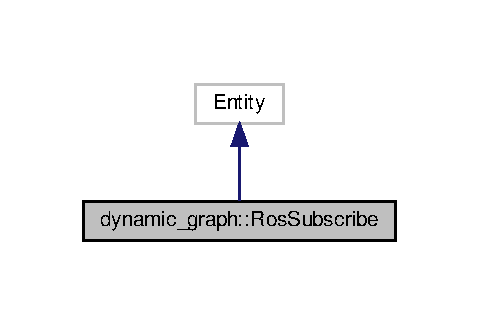
\includegraphics[width=230pt]{classdynamic__graph_1_1RosSubscribe__inherit__graph}
\end{center}
\end{figure}


Collaboration diagram for dynamic\+\_\+graph\+:\+:Ros\+Subscribe\+:
\nopagebreak
\begin{figure}[H]
\begin{center}
\leavevmode
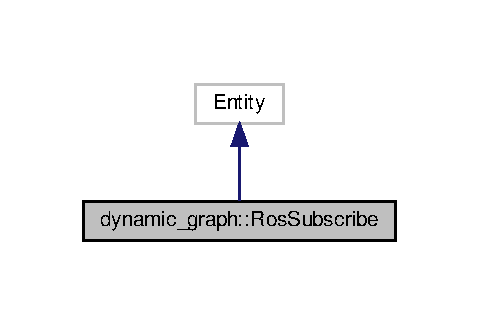
\includegraphics[width=230pt]{classdynamic__graph_1_1RosSubscribe__coll__graph}
\end{center}
\end{figure}
\subsection*{Public Types}
\begin{DoxyCompactItemize}
\item 
\mbox{\Hypertarget{classdynamic__graph_1_1RosSubscribe_a28c2e1e9ba1e6e242720086ab77e7b6f}\label{classdynamic__graph_1_1RosSubscribe_a28c2e1e9ba1e6e242720086ab77e7b6f}} 
typedef std\+::pair$<$ boost\+::shared\+\_\+ptr$<$ dynamicgraph\+::\+Signal\+Base$<$ int $>$ $>$, boost\+::shared\+\_\+ptr$<$ ros\+::\+Subscriber $>$ $>$ {\bfseries binded\+Signal\+\_\+t}
\end{DoxyCompactItemize}
\subsection*{Public Member Functions}
\begin{DoxyCompactItemize}
\item 
\mbox{\Hypertarget{classdynamic__graph_1_1RosSubscribe_ae0e13e1ae910901aed4aa3875c4cc6f8}\label{classdynamic__graph_1_1RosSubscribe_ae0e13e1ae910901aed4aa3875c4cc6f8}} 
{\bfseries Ros\+Subscribe} (const std\+::string \&n)
\item 
\mbox{\Hypertarget{classdynamic__graph_1_1RosSubscribe_a897d4b63a67fec3cb821e73697146f6b}\label{classdynamic__graph_1_1RosSubscribe_a897d4b63a67fec3cb821e73697146f6b}} 
virtual std\+::string {\bfseries get\+Doc\+String} () const
\item 
\mbox{\Hypertarget{classdynamic__graph_1_1RosSubscribe_a1aee8c0b5c13de87d42af03341fcd250}\label{classdynamic__graph_1_1RosSubscribe_a1aee8c0b5c13de87d42af03341fcd250}} 
void {\bfseries display} (std\+::ostream \&os) const
\item 
\mbox{\Hypertarget{classdynamic__graph_1_1RosSubscribe_a5ea4e0b7da520ce291a1814935b25d50}\label{classdynamic__graph_1_1RosSubscribe_a5ea4e0b7da520ce291a1814935b25d50}} 
void {\bfseries add} (const std\+::string \&signal, const std\+::string \&topic)
\item 
\mbox{\Hypertarget{classdynamic__graph_1_1RosSubscribe_a21d955435830639a8c02c4ef33c49849}\label{classdynamic__graph_1_1RosSubscribe_a21d955435830639a8c02c4ef33c49849}} 
void {\bfseries rm} (const std\+::string \&signal)
\item 
\mbox{\Hypertarget{classdynamic__graph_1_1RosSubscribe_a863629270bc4c682b45f41471f858e8c}\label{classdynamic__graph_1_1RosSubscribe_a863629270bc4c682b45f41471f858e8c}} 
std\+::string {\bfseries list} ()
\item 
\mbox{\Hypertarget{classdynamic__graph_1_1RosSubscribe_a33d08228f31cef91c35f83fee6f30bdc}\label{classdynamic__graph_1_1RosSubscribe_a33d08228f31cef91c35f83fee6f30bdc}} 
void {\bfseries clear} ()
\item 
\mbox{\Hypertarget{classdynamic__graph_1_1RosSubscribe_a4b19a0b90769381dd89c90a611fc0cbb}\label{classdynamic__graph_1_1RosSubscribe_a4b19a0b90769381dd89c90a611fc0cbb}} 
{\footnotesize template$<$typename T $>$ }\\void {\bfseries add} (const std\+::string \&signal, const std\+::string \&topic)
\item 
\mbox{\Hypertarget{classdynamic__graph_1_1RosSubscribe_a09004dab7209ce50d235295fa7c7ec0d}\label{classdynamic__graph_1_1RosSubscribe_a09004dab7209ce50d235295fa7c7ec0d}} 
std\+::map$<$ std\+::string, binded\+Signal\+\_\+t $>$ \& {\bfseries binded\+Signal} ()
\item 
\mbox{\Hypertarget{classdynamic__graph_1_1RosSubscribe_a093c394243939de8a085ae774ad05493}\label{classdynamic__graph_1_1RosSubscribe_a093c394243939de8a085ae774ad05493}} 
ros\+::\+Node\+Handle \& {\bfseries nh} ()
\item 
\mbox{\Hypertarget{classdynamic__graph_1_1RosSubscribe_acdf8089899afd8364f75ac2b70b3269f}\label{classdynamic__graph_1_1RosSubscribe_acdf8089899afd8364f75ac2b70b3269f}} 
{\footnotesize template$<$typename R , typename S $>$ }\\void {\bfseries callback} (boost\+::shared\+\_\+ptr$<$ dynamicgraph\+::\+Signal\+Ptr$<$ S, int $>$ $>$ signal, const R \&data)
\item 
\mbox{\Hypertarget{classdynamic__graph_1_1RosSubscribe_a6cb2a713a53d3cbebeeac921ba245954}\label{classdynamic__graph_1_1RosSubscribe_a6cb2a713a53d3cbebeeac921ba245954}} 
{\footnotesize template$<$typename R $>$ }\\void {\bfseries callback\+Timestamp} (boost\+::shared\+\_\+ptr$<$ dynamicgraph\+::\+Signal\+Ptr$<$ ptime, int $>$ $>$ signal, const R \&data)
\end{DoxyCompactItemize}
\subsection*{Private Types}
\begin{DoxyCompactItemize}
\item 
\mbox{\Hypertarget{classdynamic__graph_1_1RosSubscribe_a78c93ebf092b3e232d8db27e1ae0225f}\label{classdynamic__graph_1_1RosSubscribe_a78c93ebf092b3e232d8db27e1ae0225f}} 
typedef boost\+::posix\+\_\+time\+::ptime {\bfseries ptime}
\end{DoxyCompactItemize}
\subsection*{Private Member Functions}
\begin{DoxyCompactItemize}
\item 
\mbox{\Hypertarget{classdynamic__graph_1_1RosSubscribe_adb61288448d5efe7bc73cc78b9bad700}\label{classdynamic__graph_1_1RosSubscribe_adb61288448d5efe7bc73cc78b9bad700}} 
{\bfseries D\+Y\+N\+A\+M\+I\+C\+\_\+\+G\+R\+A\+P\+H\+\_\+\+E\+N\+T\+I\+T\+Y\+\_\+\+D\+E\+CL} ()
\end{DoxyCompactItemize}
\subsection*{Private Attributes}
\begin{DoxyCompactItemize}
\item 
\mbox{\Hypertarget{classdynamic__graph_1_1RosSubscribe_af3ad89b1e8e131eee45f0236c3cd0bbd}\label{classdynamic__graph_1_1RosSubscribe_af3ad89b1e8e131eee45f0236c3cd0bbd}} 
ros\+::\+Node\+Handle \& {\bfseries nh\+\_\+}
\item 
\mbox{\Hypertarget{classdynamic__graph_1_1RosSubscribe_a7f8a41ae314f370a4a33157741a2d8f1}\label{classdynamic__graph_1_1RosSubscribe_a7f8a41ae314f370a4a33157741a2d8f1}} 
std\+::map$<$ std\+::string, binded\+Signal\+\_\+t $>$ {\bfseries binded\+Signal\+\_\+}
\end{DoxyCompactItemize}
\subsection*{Static Private Attributes}
\begin{DoxyCompactItemize}
\item 
\mbox{\Hypertarget{classdynamic__graph_1_1RosSubscribe_a43579b54927302d427976ba218b2636b}\label{classdynamic__graph_1_1RosSubscribe_a43579b54927302d427976ba218b2636b}} 
static const std\+::string {\bfseries docstring\+\_\+}
\end{DoxyCompactItemize}
\subsection*{Friends}
\begin{DoxyCompactItemize}
\item 
\mbox{\Hypertarget{classdynamic__graph_1_1RosSubscribe_aff86e359edc93019ec7be05f8207a40d}\label{classdynamic__graph_1_1RosSubscribe_aff86e359edc93019ec7be05f8207a40d}} 
{\footnotesize template$<$typename T $>$ }\\class {\bfseries internal\+::\+Add}
\end{DoxyCompactItemize}


\subsection{Detailed Description}
Publish R\+OS information in the dynamic-\/graph. 

The documentation for this class was generated from the following files\+:\begin{DoxyCompactItemize}
\item 
include/ros\+\_\+entities/\hyperlink{ros__subscribe_8hh}{ros\+\_\+subscribe.\+hh}\item 
include/ros\+\_\+entities/\hyperlink{ros__subscribe_8hxx}{ros\+\_\+subscribe.\+hxx}\item 
src/ros\+\_\+entities/\hyperlink{ros__subscribe_8cpp}{ros\+\_\+subscribe.\+cpp}\end{DoxyCompactItemize}

\hypertarget{classdynamic__graph_1_1RosTfListener}{}\section{dynamic\+\_\+graph\+:\+:Ros\+Tf\+Listener Class Reference}
\label{classdynamic__graph_1_1RosTfListener}\index{dynamic\+\_\+graph\+::\+Ros\+Tf\+Listener@{dynamic\+\_\+graph\+::\+Ros\+Tf\+Listener}}


Inheritance diagram for dynamic\+\_\+graph\+:\+:Ros\+Tf\+Listener\+:\nopagebreak
\begin{figure}[H]
\begin{center}
\leavevmode
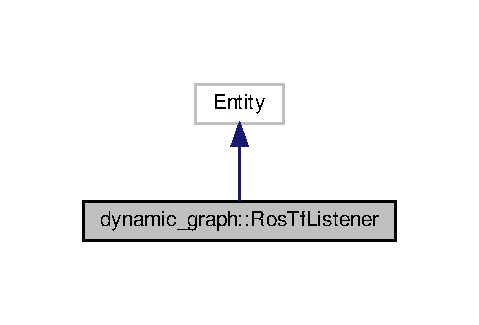
\includegraphics[width=230pt]{classdynamic__graph_1_1RosTfListener__inherit__graph}
\end{center}
\end{figure}


Collaboration diagram for dynamic\+\_\+graph\+:\+:Ros\+Tf\+Listener\+:\nopagebreak
\begin{figure}[H]
\begin{center}
\leavevmode
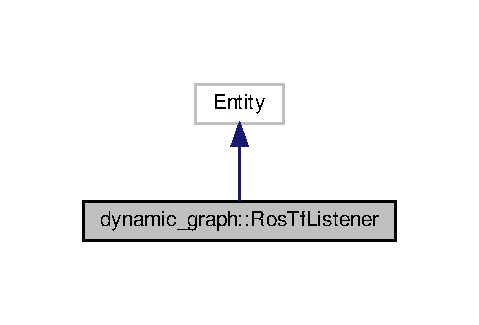
\includegraphics[width=230pt]{classdynamic__graph_1_1RosTfListener__coll__graph}
\end{center}
\end{figure}
\subsection*{Public Types}
\begin{DoxyCompactItemize}
\item 
typedef \hyperlink{structdynamic__graph_1_1internal_1_1TransformListenerData}{internal\+::\+Transform\+Listener\+Data} {\bfseries Transform\+Listener\+Data}\hypertarget{classdynamic__graph_1_1RosTfListener_acdd29e75471c27a6c4d412781254352f}{}\label{classdynamic__graph_1_1RosTfListener_acdd29e75471c27a6c4d412781254352f}

\end{DoxyCompactItemize}
\subsection*{Public Member Functions}
\begin{DoxyCompactItemize}
\item 
{\bfseries Ros\+Tf\+Listener} (const std\+::string \&name)\hypertarget{classdynamic__graph_1_1RosTfListener_a475236fb89bcd8c28b28822344f6b5da}{}\label{classdynamic__graph_1_1RosTfListener_a475236fb89bcd8c28b28822344f6b5da}

\item 
void {\bfseries add} (const std\+::string \&to, const std\+::string \&from, const std\+::string \&signame)\hypertarget{classdynamic__graph_1_1RosTfListener_ad886b7323f3f7df3171e8f3be8a7218a}{}\label{classdynamic__graph_1_1RosTfListener_ad886b7323f3f7df3171e8f3be8a7218a}

\end{DoxyCompactItemize}


The documentation for this class was generated from the following file\+:\begin{DoxyCompactItemize}
\item 
/home/mnaveau/devel/workspace/src/catkin/dg\+\_\+control/dynamic\+\_\+graph\+\_\+manager/include/ros\+\_\+entities/\hyperlink{ros__tf__listener_8hh}{ros\+\_\+tf\+\_\+listener.\+hh}\end{DoxyCompactItemize}

\hypertarget{classdynamic__graph_1_1RosTime}{}\section{dynamic\+\_\+graph\+:\+:Ros\+Time Class Reference}
\label{classdynamic__graph_1_1RosTime}\index{dynamic\+\_\+graph\+::\+Ros\+Time@{dynamic\+\_\+graph\+::\+Ros\+Time}}


Inheritance diagram for dynamic\+\_\+graph\+:\+:Ros\+Time\+:
\nopagebreak
\begin{figure}[H]
\begin{center}
\leavevmode
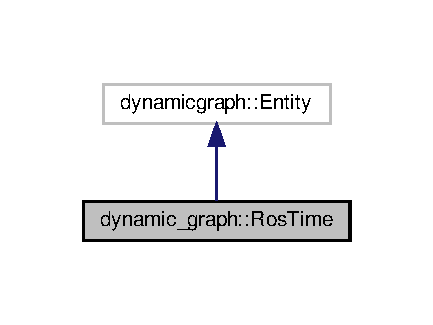
\includegraphics[width=208pt]{classdynamic__graph_1_1RosTime__inherit__graph}
\end{center}
\end{figure}


Collaboration diagram for dynamic\+\_\+graph\+:\+:Ros\+Time\+:
\nopagebreak
\begin{figure}[H]
\begin{center}
\leavevmode
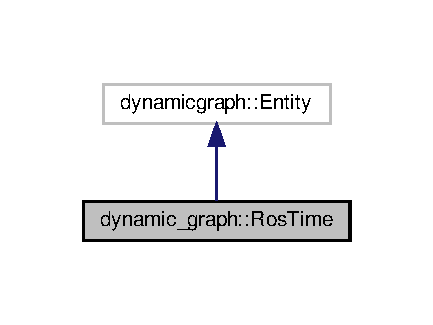
\includegraphics[width=208pt]{classdynamic__graph_1_1RosTime__coll__graph}
\end{center}
\end{figure}
\subsection*{Public Member Functions}
\begin{DoxyCompactItemize}
\item 
{\bfseries Ros\+Time} (const std\+::string \&name)\hypertarget{classdynamic__graph_1_1RosTime_aa909f2b766b54a543a59ae8642db3bc0}{}\label{classdynamic__graph_1_1RosTime_aa909f2b766b54a543a59ae8642db3bc0}

\item 
virtual std\+::string {\bfseries get\+Doc\+String} () const \hypertarget{classdynamic__graph_1_1RosTime_ad82554947f14f37bc07ccdfde068a3e6}{}\label{classdynamic__graph_1_1RosTime_ad82554947f14f37bc07ccdfde068a3e6}

\end{DoxyCompactItemize}
\subsection*{Public Attributes}
\begin{DoxyCompactItemize}
\item 
dynamicgraph\+::\+Signal$<$ boost\+::posix\+\_\+time\+::ptime, int $>$ {\bfseries now\+\_\+}\hypertarget{classdynamic__graph_1_1RosTime_ac928e12f6defd2dbda5827010fa073b7}{}\label{classdynamic__graph_1_1RosTime_ac928e12f6defd2dbda5827010fa073b7}

\end{DoxyCompactItemize}
\subsection*{Protected Member Functions}
\begin{DoxyCompactItemize}
\item 
boost\+::posix\+\_\+time\+::ptime \& {\bfseries update} (boost\+::posix\+\_\+time\+::ptime \&time, const int \&t)\hypertarget{classdynamic__graph_1_1RosTime_a29444845a864140359ec5c77169f638d}{}\label{classdynamic__graph_1_1RosTime_a29444845a864140359ec5c77169f638d}

\end{DoxyCompactItemize}
\subsection*{Private Member Functions}
\begin{DoxyCompactItemize}
\item 
{\bfseries D\+Y\+N\+A\+M\+I\+C\+\_\+\+G\+R\+A\+P\+H\+\_\+\+E\+N\+T\+I\+T\+Y\+\_\+\+D\+E\+CL} ()\hypertarget{classdynamic__graph_1_1RosTime_ad4c1f7551d8f63129ecb6e6ecaf828e6}{}\label{classdynamic__graph_1_1RosTime_ad4c1f7551d8f63129ecb6e6ecaf828e6}

\end{DoxyCompactItemize}
\subsection*{Static Private Attributes}
\begin{DoxyCompactItemize}
\item 
static const std\+::string {\bfseries docstring\+\_\+}\hypertarget{classdynamic__graph_1_1RosTime_a41b421e48816fc5533e2190124f6f48d}{}\label{classdynamic__graph_1_1RosTime_a41b421e48816fc5533e2190124f6f48d}

\end{DoxyCompactItemize}


The documentation for this class was generated from the following files\+:\begin{DoxyCompactItemize}
\item 
include/ros\+\_\+entities/\hyperlink{ros__time_8hh}{ros\+\_\+time.\+hh}\item 
src/ros\+\_\+entities/\hyperlink{ros__time_8cpp}{ros\+\_\+time.\+cpp}\end{DoxyCompactItemize}

\hypertarget{structdynamic__graph_1_1PeriodicCall_1_1SignalToCall}{}\section{dynamic\+\_\+graph\+:\+:Periodic\+Call\+:\+:Signal\+To\+Call Struct Reference}
\label{structdynamic__graph_1_1PeriodicCall_1_1SignalToCall}\index{dynamic\+\_\+graph\+::\+Periodic\+Call\+::\+Signal\+To\+Call@{dynamic\+\_\+graph\+::\+Periodic\+Call\+::\+Signal\+To\+Call}}
\subsection*{Public Member Functions}
\begin{DoxyCompactItemize}
\item 
\mbox{\Hypertarget{structdynamic__graph_1_1PeriodicCall_1_1SignalToCall_a9efbb8370bdb3ebadb9ee9e8f4a6c209}\label{structdynamic__graph_1_1PeriodicCall_1_1SignalToCall_a9efbb8370bdb3ebadb9ee9e8f4a6c209}} 
{\bfseries Signal\+To\+Call} (dynamicgraph\+::\+Signal\+Base$<$ int $>$ $\ast$s, unsigned int df=1)
\end{DoxyCompactItemize}
\subsection*{Public Attributes}
\begin{DoxyCompactItemize}
\item 
\mbox{\Hypertarget{structdynamic__graph_1_1PeriodicCall_1_1SignalToCall_aa4ca46512452a1107926da8a92803597}\label{structdynamic__graph_1_1PeriodicCall_1_1SignalToCall_aa4ca46512452a1107926da8a92803597}} 
dynamicgraph\+::\+Signal\+Base$<$ int $>$ $\ast$ {\bfseries signal\+\_\+}
\item 
\mbox{\Hypertarget{structdynamic__graph_1_1PeriodicCall_1_1SignalToCall_aae29661d7a6753e2bd60565ce2a7d146}\label{structdynamic__graph_1_1PeriodicCall_1_1SignalToCall_aae29661d7a6753e2bd60565ce2a7d146}} 
unsigned int {\bfseries down\+\_\+sampling\+\_\+factor\+\_\+}
\end{DoxyCompactItemize}


The documentation for this struct was generated from the following file\+:\begin{DoxyCompactItemize}
\item 
include/dynamic\+\_\+graph\+\_\+manager/\hyperlink{periodic-call_8hh}{periodic-\/call.\+hh}\end{DoxyCompactItemize}

\hypertarget{classdynamic__graph__manager_1_1SimpleDGM}{}\section{dynamic\+\_\+graph\+\_\+manager\+:\+:Simple\+D\+GM Class Reference}
\label{classdynamic__graph__manager_1_1SimpleDGM}\index{dynamic\+\_\+graph\+\_\+manager\+::\+Simple\+D\+GM@{dynamic\+\_\+graph\+\_\+manager\+::\+Simple\+D\+GM}}


This class is a simple dynamic graph manager with a fake hardware interface used for unittesting.  




{\ttfamily \#include $<$simple\+\_\+dgm.\+hpp$>$}



Inheritance diagram for dynamic\+\_\+graph\+\_\+manager\+:\+:Simple\+D\+GM\+:
\nopagebreak
\begin{figure}[H]
\begin{center}
\leavevmode
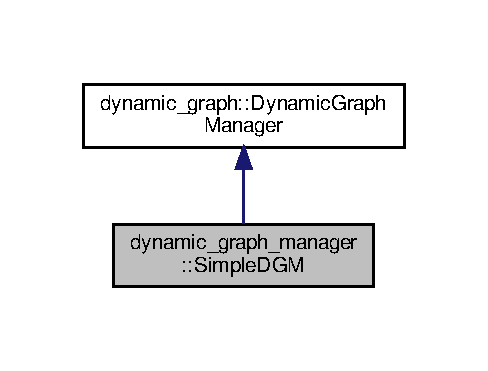
\includegraphics[width=234pt]{classdynamic__graph__manager_1_1SimpleDGM__inherit__graph}
\end{center}
\end{figure}


Collaboration diagram for dynamic\+\_\+graph\+\_\+manager\+:\+:Simple\+D\+GM\+:
\nopagebreak
\begin{figure}[H]
\begin{center}
\leavevmode
\includegraphics[width=234pt]{classdynamic__graph__manager_1_1SimpleDGM__coll__graph}
\end{center}
\end{figure}
\subsection*{Public Member Functions}
\begin{DoxyCompactItemize}
\item 
\mbox{\Hypertarget{classdynamic__graph__manager_1_1SimpleDGM_abb548458a154ee8e9ae63a32f1191ef6}\label{classdynamic__graph__manager_1_1SimpleDGM_abb548458a154ee8e9ae63a32f1191ef6}} 
\hyperlink{classdynamic__graph__manager_1_1SimpleDGM_abb548458a154ee8e9ae63a32f1191ef6}{Simple\+D\+GM} ()
\begin{DoxyCompactList}\small\item\em Construct a new \hyperlink{classdynamic__graph__manager_1_1SimpleDGM}{Simple\+D\+GM} object. \end{DoxyCompactList}\item 
\mbox{\Hypertarget{classdynamic__graph__manager_1_1SimpleDGM_a250f18b97619c72446074662626423d4}\label{classdynamic__graph__manager_1_1SimpleDGM_a250f18b97619c72446074662626423d4}} 
\hyperlink{classdynamic__graph__manager_1_1SimpleDGM_a250f18b97619c72446074662626423d4}{$\sim$\+Simple\+D\+GM} ()
\begin{DoxyCompactList}\small\item\em Destroy the \hyperlink{classdynamic__graph__manager_1_1SimpleDGM}{Simple\+D\+GM} object. \end{DoxyCompactList}\item 
void \hyperlink{classdynamic__graph__manager_1_1SimpleDGM_a5d771fc5a9ae6dd524a658d50fbee5d3}{initialize\+\_\+hardware\+\_\+communication\+\_\+process} ()
\begin{DoxyCompactList}\small\item\em Simple overload doing nothing. \end{DoxyCompactList}\item 
void \hyperlink{classdynamic__graph__manager_1_1SimpleDGM_aa92cd33a31c934835252f834bab7b9f4}{get\+\_\+sensors\+\_\+to\+\_\+map} (\hyperlink{namespacedynamic__graph_a51212ed7fa4ae81e7b362a27f09b7ab8}{dynamic\+\_\+graph\+::\+Vector\+D\+G\+Map} \&map)
\begin{DoxyCompactList}\small\item\em Get the sensors to the map object. \end{DoxyCompactList}\item 
void \hyperlink{classdynamic__graph__manager_1_1SimpleDGM_ad38ccd35cc0c409a0aaefa8565634109}{set\+\_\+motor\+\_\+controls\+\_\+from\+\_\+map} (const \hyperlink{namespacedynamic__graph_a51212ed7fa4ae81e7b362a27f09b7ab8}{dynamic\+\_\+graph\+::\+Vector\+D\+G\+Map} \&map)
\begin{DoxyCompactList}\small\item\em Set the motor controls from map object to no hardware. \end{DoxyCompactList}\item 
\mbox{\Hypertarget{classdynamic__graph__manager_1_1SimpleDGM_a08793eb7410b2820e00e028688d890a9}\label{classdynamic__graph__manager_1_1SimpleDGM_a08793eb7410b2820e00e028688d890a9}} 
bool \hyperlink{classdynamic__graph__manager_1_1SimpleDGM_a08793eb7410b2820e00e028688d890a9}{get\+\_\+has\+\_\+user\+\_\+command\+\_\+been\+\_\+executed} ()
\begin{DoxyCompactList}\small\item\em Get the has\+\_\+user\+\_\+command\+\_\+been\+\_\+executed\+\_\+ object. \end{DoxyCompactList}\item 
bool \hyperlink{classdynamic__graph__manager_1_1SimpleDGM_adb40055a916691d326bc6466eab9680b}{user\+\_\+command\+\_\+callback} (dynamic\+\_\+graph\+\_\+manager\+::\+Test\+User\+Cmd\+Bool\+::\+Request \&req, dynamic\+\_\+graph\+\_\+manager\+::\+Test\+User\+Cmd\+Bool\+::\+Response \&res)
\begin{DoxyCompactList}\small\item\em This service callback parse the ros messages and register and internal method for further call using the data from the ros message. \end{DoxyCompactList}\item 
bool \hyperlink{classdynamic__graph__manager_1_1SimpleDGM_a5fe81f9feb5d982761d7a427aa31e7b4}{is\+\_\+in\+\_\+safety\+\_\+mode} ()
\begin{DoxyCompactList}\small\item\em is\+\_\+in\+\_\+safety\+\_\+mode check if the dynamic graph is still alive and sending commands at a descent frequency. \end{DoxyCompactList}\item 
\mbox{\Hypertarget{classdynamic__graph__manager_1_1SimpleDGM_a37b28e687ce4e724770f5c9f23da4d4f}\label{classdynamic__graph__manager_1_1SimpleDGM_a37b28e687ce4e724770f5c9f23da4d4f}} 
void \hyperlink{classdynamic__graph__manager_1_1SimpleDGM_a37b28e687ce4e724770f5c9f23da4d4f}{compute\+\_\+safety\+\_\+controls} ()
\begin{DoxyCompactList}\small\item\em compute\+\_\+safety\+\_\+controls computes safety controls very fast in case the dynamic graph is taking to much computation time or has crashed. \end{DoxyCompactList}\end{DoxyCompactItemize}
\subsection*{Private Member Functions}
\begin{DoxyCompactItemize}
\item 
void \hyperlink{classdynamic__graph__manager_1_1SimpleDGM_a6ba8314169c29c722cdcea810798f08d}{user\+\_\+command} (bool user\+\_\+input)
\begin{DoxyCompactList}\small\item\em The actuall user command called in the real time thread. \end{DoxyCompactList}\end{DoxyCompactItemize}
\subsection*{Private Attributes}
\begin{DoxyCompactItemize}
\item 
\mbox{\Hypertarget{classdynamic__graph__manager_1_1SimpleDGM_aa8dfcc77796249b13b61b7a3c4a54d3e}\label{classdynamic__graph__manager_1_1SimpleDGM_aa8dfcc77796249b13b61b7a3c4a54d3e}} 
std\+::atomic\+\_\+bool {\bfseries boolean\+\_\+set\+\_\+by\+\_\+user\+\_\+cmd\+\_\+}
\item 
\mbox{\Hypertarget{classdynamic__graph__manager_1_1SimpleDGM_a4bebf8a5b309160a26bfcc9c1f18f9df}\label{classdynamic__graph__manager_1_1SimpleDGM_a4bebf8a5b309160a26bfcc9c1f18f9df}} 
dynamicgraph\+::\+Vector {\bfseries desired\+\_\+torques\+\_\+}
\item 
\mbox{\Hypertarget{classdynamic__graph__manager_1_1SimpleDGM_a46ad5e1d2ac144f8bc799480b6dfda45}\label{classdynamic__graph__manager_1_1SimpleDGM_a46ad5e1d2ac144f8bc799480b6dfda45}} 
dynamicgraph\+::\+Vector {\bfseries desired\+\_\+positions\+\_\+}
\end{DoxyCompactItemize}
\subsection*{Additional Inherited Members}


\subsection{Detailed Description}
This class is a simple dynamic graph manager with a fake hardware interface used for unittesting. \begin{Desc}
\item[Examples\+: ]\par
\hyperlink{main_8cpp-example}{main.\+cpp}.\end{Desc}


\subsection{Member Function Documentation}
\mbox{\Hypertarget{classdynamic__graph__manager_1_1SimpleDGM_aa92cd33a31c934835252f834bab7b9f4}\label{classdynamic__graph__manager_1_1SimpleDGM_aa92cd33a31c934835252f834bab7b9f4}} 
\index{dynamic\+\_\+graph\+\_\+manager\+::\+Simple\+D\+GM@{dynamic\+\_\+graph\+\_\+manager\+::\+Simple\+D\+GM}!get\+\_\+sensors\+\_\+to\+\_\+map@{get\+\_\+sensors\+\_\+to\+\_\+map}}
\index{get\+\_\+sensors\+\_\+to\+\_\+map@{get\+\_\+sensors\+\_\+to\+\_\+map}!dynamic\+\_\+graph\+\_\+manager\+::\+Simple\+D\+GM@{dynamic\+\_\+graph\+\_\+manager\+::\+Simple\+D\+GM}}
\subsubsection{\texorpdfstring{get\+\_\+sensors\+\_\+to\+\_\+map()}{get\_sensors\_to\_map()}}
{\footnotesize\ttfamily void dynamic\+\_\+graph\+\_\+manager\+::\+Simple\+D\+G\+M\+::get\+\_\+sensors\+\_\+to\+\_\+map (\begin{DoxyParamCaption}\item[{\hyperlink{namespacedynamic__graph_a51212ed7fa4ae81e7b362a27f09b7ab8}{dynamic\+\_\+graph\+::\+Vector\+D\+G\+Map} \&}]{map }\end{DoxyParamCaption})\hspace{0.3cm}{\ttfamily [inline]}, {\ttfamily [virtual]}}



Get the sensors to the map object. 


\begin{DoxyParams}{Parameters}
{\em map} & of sensors \\
\hline
\end{DoxyParams}


Reimplemented from \hyperlink{classdynamic__graph_1_1DynamicGraphManager_a7bddce83d5185433041ad27610b85b3a}{dynamic\+\_\+graph\+::\+Dynamic\+Graph\+Manager}.

\begin{Desc}
\item[Examples\+: ]\par
\hyperlink{simple_dgm_8hpp-example}{simple\+\_\+dgm.\+hpp}.\end{Desc}
\mbox{\Hypertarget{classdynamic__graph__manager_1_1SimpleDGM_a5d771fc5a9ae6dd524a658d50fbee5d3}\label{classdynamic__graph__manager_1_1SimpleDGM_a5d771fc5a9ae6dd524a658d50fbee5d3}} 
\index{dynamic\+\_\+graph\+\_\+manager\+::\+Simple\+D\+GM@{dynamic\+\_\+graph\+\_\+manager\+::\+Simple\+D\+GM}!initialize\+\_\+hardware\+\_\+communication\+\_\+process@{initialize\+\_\+hardware\+\_\+communication\+\_\+process}}
\index{initialize\+\_\+hardware\+\_\+communication\+\_\+process@{initialize\+\_\+hardware\+\_\+communication\+\_\+process}!dynamic\+\_\+graph\+\_\+manager\+::\+Simple\+D\+GM@{dynamic\+\_\+graph\+\_\+manager\+::\+Simple\+D\+GM}}
\subsubsection{\texorpdfstring{initialize\+\_\+hardware\+\_\+communication\+\_\+process()}{initialize\_hardware\_communication\_process()}}
{\footnotesize\ttfamily void dynamic\+\_\+graph\+\_\+manager\+::\+Simple\+D\+G\+M\+::initialize\+\_\+hardware\+\_\+communication\+\_\+process (\begin{DoxyParamCaption}{ }\end{DoxyParamCaption})\hspace{0.3cm}{\ttfamily [inline]}, {\ttfamily [virtual]}}



Simple overload doing nothing. 

We have no hardware here for the unit tests. initialize the user commands 

Reimplemented from \hyperlink{classdynamic__graph_1_1DynamicGraphManager_ae3927887762c52c7bf50ab5a565c3077}{dynamic\+\_\+graph\+::\+Dynamic\+Graph\+Manager}.

\begin{Desc}
\item[Examples\+: ]\par
\hyperlink{simple_dgm_8hpp-example}{simple\+\_\+dgm.\+hpp}.\end{Desc}
\mbox{\Hypertarget{classdynamic__graph__manager_1_1SimpleDGM_a5fe81f9feb5d982761d7a427aa31e7b4}\label{classdynamic__graph__manager_1_1SimpleDGM_a5fe81f9feb5d982761d7a427aa31e7b4}} 
\index{dynamic\+\_\+graph\+\_\+manager\+::\+Simple\+D\+GM@{dynamic\+\_\+graph\+\_\+manager\+::\+Simple\+D\+GM}!is\+\_\+in\+\_\+safety\+\_\+mode@{is\+\_\+in\+\_\+safety\+\_\+mode}}
\index{is\+\_\+in\+\_\+safety\+\_\+mode@{is\+\_\+in\+\_\+safety\+\_\+mode}!dynamic\+\_\+graph\+\_\+manager\+::\+Simple\+D\+GM@{dynamic\+\_\+graph\+\_\+manager\+::\+Simple\+D\+GM}}
\subsubsection{\texorpdfstring{is\+\_\+in\+\_\+safety\+\_\+mode()}{is\_in\_safety\_mode()}}
{\footnotesize\ttfamily bool dynamic\+\_\+graph\+\_\+manager\+::\+Simple\+D\+G\+M\+::is\+\_\+in\+\_\+safety\+\_\+mode (\begin{DoxyParamCaption}{ }\end{DoxyParamCaption})\hspace{0.3cm}{\ttfamily [inline]}, {\ttfamily [virtual]}}



is\+\_\+in\+\_\+safety\+\_\+mode check if the dynamic graph is still alive and sending commands at a descent frequency. 

Inheriting this method is not mandatory but recommanded. \begin{DoxyReturn}{Returns}
true if there is a problem 
\end{DoxyReturn}


Reimplemented from \hyperlink{classdynamic__graph_1_1DynamicGraphManager_aea29e8dc351e0a50a8d2803d854d238d}{dynamic\+\_\+graph\+::\+Dynamic\+Graph\+Manager}.

\begin{Desc}
\item[Examples\+: ]\par
\hyperlink{simple_dgm_8hpp-example}{simple\+\_\+dgm.\+hpp}.\end{Desc}
\mbox{\Hypertarget{classdynamic__graph__manager_1_1SimpleDGM_ad38ccd35cc0c409a0aaefa8565634109}\label{classdynamic__graph__manager_1_1SimpleDGM_ad38ccd35cc0c409a0aaefa8565634109}} 
\index{dynamic\+\_\+graph\+\_\+manager\+::\+Simple\+D\+GM@{dynamic\+\_\+graph\+\_\+manager\+::\+Simple\+D\+GM}!set\+\_\+motor\+\_\+controls\+\_\+from\+\_\+map@{set\+\_\+motor\+\_\+controls\+\_\+from\+\_\+map}}
\index{set\+\_\+motor\+\_\+controls\+\_\+from\+\_\+map@{set\+\_\+motor\+\_\+controls\+\_\+from\+\_\+map}!dynamic\+\_\+graph\+\_\+manager\+::\+Simple\+D\+GM@{dynamic\+\_\+graph\+\_\+manager\+::\+Simple\+D\+GM}}
\subsubsection{\texorpdfstring{set\+\_\+motor\+\_\+controls\+\_\+from\+\_\+map()}{set\_motor\_controls\_from\_map()}}
{\footnotesize\ttfamily void dynamic\+\_\+graph\+\_\+manager\+::\+Simple\+D\+G\+M\+::set\+\_\+motor\+\_\+controls\+\_\+from\+\_\+map (\begin{DoxyParamCaption}\item[{const \hyperlink{namespacedynamic__graph_a51212ed7fa4ae81e7b362a27f09b7ab8}{dynamic\+\_\+graph\+::\+Vector\+D\+G\+Map} \&}]{map }\end{DoxyParamCaption})\hspace{0.3cm}{\ttfamily [inline]}, {\ttfamily [virtual]}}



Set the motor controls from map object to no hardware. 

So nothing to be done here


\begin{DoxyParams}{Parameters}
{\em map} & of controls \\
\hline
\end{DoxyParams}


Reimplemented from \hyperlink{classdynamic__graph_1_1DynamicGraphManager_a506e6f37ac7205efaf0efe4202cde897}{dynamic\+\_\+graph\+::\+Dynamic\+Graph\+Manager}.

\begin{Desc}
\item[Examples\+: ]\par
\hyperlink{simple_dgm_8hpp-example}{simple\+\_\+dgm.\+hpp}.\end{Desc}
\mbox{\Hypertarget{classdynamic__graph__manager_1_1SimpleDGM_a6ba8314169c29c722cdcea810798f08d}\label{classdynamic__graph__manager_1_1SimpleDGM_a6ba8314169c29c722cdcea810798f08d}} 
\index{dynamic\+\_\+graph\+\_\+manager\+::\+Simple\+D\+GM@{dynamic\+\_\+graph\+\_\+manager\+::\+Simple\+D\+GM}!user\+\_\+command@{user\+\_\+command}}
\index{user\+\_\+command@{user\+\_\+command}!dynamic\+\_\+graph\+\_\+manager\+::\+Simple\+D\+GM@{dynamic\+\_\+graph\+\_\+manager\+::\+Simple\+D\+GM}}
\subsubsection{\texorpdfstring{user\+\_\+command()}{user\_command()}}
{\footnotesize\ttfamily void dynamic\+\_\+graph\+\_\+manager\+::\+Simple\+D\+G\+M\+::user\+\_\+command (\begin{DoxyParamCaption}\item[{bool}]{user\+\_\+input }\end{DoxyParamCaption})\hspace{0.3cm}{\ttfamily [inline]}, {\ttfamily [private]}}



The actuall user command called in the real time thread. 


\begin{DoxyParams}{Parameters}
{\em user\+\_\+input} & is some boolean \\
\hline
\end{DoxyParams}
\begin{Desc}
\item[Examples\+: ]\par
\hyperlink{simple_dgm_8hpp-example}{simple\+\_\+dgm.\+hpp}.\end{Desc}
\mbox{\Hypertarget{classdynamic__graph__manager_1_1SimpleDGM_adb40055a916691d326bc6466eab9680b}\label{classdynamic__graph__manager_1_1SimpleDGM_adb40055a916691d326bc6466eab9680b}} 
\index{dynamic\+\_\+graph\+\_\+manager\+::\+Simple\+D\+GM@{dynamic\+\_\+graph\+\_\+manager\+::\+Simple\+D\+GM}!user\+\_\+command\+\_\+callback@{user\+\_\+command\+\_\+callback}}
\index{user\+\_\+command\+\_\+callback@{user\+\_\+command\+\_\+callback}!dynamic\+\_\+graph\+\_\+manager\+::\+Simple\+D\+GM@{dynamic\+\_\+graph\+\_\+manager\+::\+Simple\+D\+GM}}
\subsubsection{\texorpdfstring{user\+\_\+command\+\_\+callback()}{user\_command\_callback()}}
{\footnotesize\ttfamily bool dynamic\+\_\+graph\+\_\+manager\+::\+Simple\+D\+G\+M\+::user\+\_\+command\+\_\+callback (\begin{DoxyParamCaption}\item[{dynamic\+\_\+graph\+\_\+manager\+::\+Test\+User\+Cmd\+Bool\+::\+Request \&}]{req,  }\item[{dynamic\+\_\+graph\+\_\+manager\+::\+Test\+User\+Cmd\+Bool\+::\+Response \&}]{res }\end{DoxyParamCaption})\hspace{0.3cm}{\ttfamily [inline]}}



This service callback parse the ros messages and register and internal method for further call using the data from the ros message. 


\begin{DoxyParams}{Parameters}
{\em req} & this is the user argument \\
\hline
{\em res} & this is the feedback of the user command \\
\hline
\end{DoxyParams}
\begin{DoxyReturn}{Returns}
true in case the service hase been properly executed 

false in case of failure 
\end{DoxyReturn}
\begin{Desc}
\item[Examples\+: ]\par
\hyperlink{simple_dgm_8hpp-example}{simple\+\_\+dgm.\+hpp}.\end{Desc}


The documentation for this class was generated from the following file\+:\begin{DoxyCompactItemize}
\item 
demos/\hyperlink{simple__dgm_8hpp}{simple\+\_\+dgm.\+hpp}\end{DoxyCompactItemize}

\hypertarget{structdynamic__graph_1_1internal_1_1TransformListenerData}{}\section{dynamic\+\_\+graph\+:\+:internal\+:\+:Transform\+Listener\+Data Struct Reference}
\label{structdynamic__graph_1_1internal_1_1TransformListenerData}\index{dynamic\+\_\+graph\+::internal\+::\+Transform\+Listener\+Data@{dynamic\+\_\+graph\+::internal\+::\+Transform\+Listener\+Data}}
\subsection*{Public Types}
\begin{DoxyCompactItemize}
\item 
\mbox{\Hypertarget{structdynamic__graph_1_1internal_1_1TransformListenerData_ac6a6174f637f20a2fd08505f8384ffeb}\label{structdynamic__graph_1_1internal_1_1TransformListenerData_ac6a6174f637f20a2fd08505f8384ffeb}} 
typedef dynamicgraph\+::\+Signal$<$ Matrix\+Homogeneous, int $>$ {\bfseries signal\+\_\+t}
\end{DoxyCompactItemize}
\subsection*{Public Member Functions}
\begin{DoxyCompactItemize}
\item 
\mbox{\Hypertarget{structdynamic__graph_1_1internal_1_1TransformListenerData_aea741575414599c63429b551de15c17b}\label{structdynamic__graph_1_1internal_1_1TransformListenerData_aea741575414599c63429b551de15c17b}} 
{\bfseries Transform\+Listener\+Data} (tf\+::\+Transform\+Listener \&l, const std\+::string \&to, const std\+::string \&from, const std\+::string \&signame)
\item 
\mbox{\Hypertarget{structdynamic__graph_1_1internal_1_1TransformListenerData_abbb4ba6133c60d3b39a1a078acce7bb2}\label{structdynamic__graph_1_1internal_1_1TransformListenerData_abbb4ba6133c60d3b39a1a078acce7bb2}} 
Matrix\+Homogeneous \& {\bfseries get\+Transform} (Matrix\+Homogeneous \&res, int time)
\end{DoxyCompactItemize}
\subsection*{Public Attributes}
\begin{DoxyCompactItemize}
\item 
\mbox{\Hypertarget{structdynamic__graph_1_1internal_1_1TransformListenerData_ae83ed824d8e7350c639d3a4b8f8c7c51}\label{structdynamic__graph_1_1internal_1_1TransformListenerData_ae83ed824d8e7350c639d3a4b8f8c7c51}} 
tf\+::\+Transform\+Listener \& {\bfseries listener}
\item 
\mbox{\Hypertarget{structdynamic__graph_1_1internal_1_1TransformListenerData_a35c066b704b49bad5319aeefd6955edf}\label{structdynamic__graph_1_1internal_1_1TransformListenerData_a35c066b704b49bad5319aeefd6955edf}} 
const std\+::string {\bfseries to\+Frame}
\item 
\mbox{\Hypertarget{structdynamic__graph_1_1internal_1_1TransformListenerData_a95d5dd80a8b2eb36e42515c5e20ea514}\label{structdynamic__graph_1_1internal_1_1TransformListenerData_a95d5dd80a8b2eb36e42515c5e20ea514}} 
const std\+::string {\bfseries from\+Frame}
\item 
\mbox{\Hypertarget{structdynamic__graph_1_1internal_1_1TransformListenerData_a79d1956bbae0f50368633551cee1995b}\label{structdynamic__graph_1_1internal_1_1TransformListenerData_a79d1956bbae0f50368633551cee1995b}} 
tf\+::\+Stamped\+Transform {\bfseries transform}
\item 
\mbox{\Hypertarget{structdynamic__graph_1_1internal_1_1TransformListenerData_aa8e36737907c1f68321dd2535cf11620}\label{structdynamic__graph_1_1internal_1_1TransformListenerData_aa8e36737907c1f68321dd2535cf11620}} 
signal\+\_\+t {\bfseries signal}
\end{DoxyCompactItemize}


The documentation for this struct was generated from the following file\+:\begin{DoxyCompactItemize}
\item 
include/ros\+\_\+entities/\hyperlink{ros__tf__listener_8hh}{ros\+\_\+tf\+\_\+listener.\+hh}\end{DoxyCompactItemize}

\hypertarget{classdynamic__graph_1_1specific_1_1Twist}{}\section{dynamic\+\_\+graph\+:\+:specific\+:\+:Twist Class Reference}
\label{classdynamic__graph_1_1specific_1_1Twist}\index{dynamic\+\_\+graph\+::specific\+::\+Twist@{dynamic\+\_\+graph\+::specific\+::\+Twist}}


The documentation for this class was generated from the following file\+:\begin{DoxyCompactItemize}
\item 
/home/mnaveau/devel/workspace/src/catkin/dg\+\_\+control/dynamic\+\_\+graph\+\_\+manager/include/ros\+\_\+entities/\hyperlink{dg__to__ros_8hh}{dg\+\_\+to\+\_\+ros.\+hh}\end{DoxyCompactItemize}

\hypertarget{classdynamic__graph_1_1specific_1_1Vector3}{}\section{dynamic\+\_\+graph\+:\+:specific\+:\+:Vector3 Class Reference}
\label{classdynamic__graph_1_1specific_1_1Vector3}\index{dynamic\+\_\+graph\+::specific\+::\+Vector3@{dynamic\+\_\+graph\+::specific\+::\+Vector3}}


The documentation for this class was generated from the following file\+:\begin{DoxyCompactItemize}
\item 
/home/mnaveau/devel/workspace/src/catkin/dg\+\_\+control/dynamic\+\_\+graph\+\_\+manager/include/ros\+\_\+entities/\hyperlink{dg__to__ros_8hh}{dg\+\_\+to\+\_\+ros.\+hh}\end{DoxyCompactItemize}

\chapter{File Documentation}
\hypertarget{main_8cpp}{}\section{benchmarks/main.cpp File Reference}
\label{main_8cpp}\index{benchmarks/main.\+cpp@{benchmarks/main.\+cpp}}


Initialize and run unittest using the google suit.  


{\ttfamily \#include \char`\"{}gtest/gtest.\+h\char`\"{}}\newline
Include dependency graph for main.\+cpp\+:
\nopagebreak
\begin{figure}[H]
\begin{center}
\leavevmode
\includegraphics[width=193pt]{main_8cpp__incl}
\end{center}
\end{figure}
\subsection*{Functions}
\begin{DoxyCompactItemize}
\item 
\mbox{\Hypertarget{main_8cpp_a3c04138a5bfe5d72780bb7e82a18e627}\label{main_8cpp_a3c04138a5bfe5d72780bb7e82a18e627}} 
int {\bfseries main} (int argc, char $\ast$$\ast$argv)
\end{DoxyCompactItemize}


\subsection{Detailed Description}
Initialize and run unittest using the google suit. 

\begin{DoxyAuthor}{Author}
Vincent Berenz 
\end{DoxyAuthor}
\begin{DoxyRefDesc}{License}
\item[\hyperlink{license__license000002}{License}]License B\+S\+D-\/3-\/\+Clause \end{DoxyRefDesc}
\begin{DoxyCopyright}{Copyright}
Copyright (c) 2019, New York University and Max Planck Gesellschaft. 
\end{DoxyCopyright}
\begin{DoxyDate}{Date}
2019-\/05-\/22 
\end{DoxyDate}

\hypertarget{simple__dgm_8hpp}{}\section{demos/simple\+\_\+dgm.hpp File Reference}
\label{simple__dgm_8hpp}\index{demos/simple\+\_\+dgm.\+hpp@{demos/simple\+\_\+dgm.\+hpp}}
{\ttfamily \#include \char`\"{}dynamic\+\_\+graph\+\_\+manager/ros\+\_\+init.\+hh\char`\"{}}\\*
{\ttfamily \#include \char`\"{}dynamic\+\_\+graph\+\_\+manager/dynamic\+\_\+graph\+\_\+manager.\+hh\char`\"{}}\\*
{\ttfamily \#include \char`\"{}dynamic\+\_\+graph\+\_\+manager/\+Test\+User\+Cmd\+Bool.\+h\char`\"{}}\\*
Include dependency graph for simple\+\_\+dgm.\+hpp\+:
\nopagebreak
\begin{figure}[H]
\begin{center}
\leavevmode
\includegraphics[width=350pt]{simple__dgm_8hpp__incl}
\end{center}
\end{figure}
This graph shows which files directly or indirectly include this file\+:
\nopagebreak
\begin{figure}[H]
\begin{center}
\leavevmode
\includegraphics[width=200pt]{simple__dgm_8hpp__dep__incl}
\end{center}
\end{figure}
\subsection*{Classes}
\begin{DoxyCompactItemize}
\item 
class \hyperlink{classdynamic__graph__manager_1_1SimpleDGM}{dynamic\+\_\+graph\+\_\+manager\+::\+Simple\+D\+GM}
\begin{DoxyCompactList}\small\item\em This class is a simple dynamic graph manager with a fake hardware interface used for unittesting. \end{DoxyCompactList}\end{DoxyCompactItemize}
\subsection*{Namespaces}
\begin{DoxyCompactItemize}
\item 
 \hyperlink{namespacedynamic__graph__manager}{dynamic\+\_\+graph\+\_\+manager}
\begin{DoxyCompactList}\small\item\em Example of hardware communication client based on R\+OS. \end{DoxyCompactList}\end{DoxyCompactItemize}


\subsection{Detailed Description}
\begin{DoxyAuthor}{Author}
Maximilien Naveau (\href{mailto:maximilien.naveau@gmail.com}{\tt maximilien.\+naveau@gmail.\+com}) 
\end{DoxyAuthor}
\begin{DoxyRefDesc}{License}
\item[\hyperlink{license__license000002}{License}]License B\+S\+D-\/3-\/\+Clause \end{DoxyRefDesc}
\begin{DoxyCopyright}{Copyright}
Copyright (c) 2019, New York University and Max Planck Gesellschaft. 
\end{DoxyCopyright}
\begin{DoxyDate}{Date}
2019-\/05-\/22 
\end{DoxyDate}

\hypertarget{device_8hh}{}\section{include/dynamic\+\_\+graph\+\_\+manager/device.hh File Reference}
\label{device_8hh}\index{include/dynamic\+\_\+graph\+\_\+manager/device.\+hh@{include/dynamic\+\_\+graph\+\_\+manager/device.\+hh}}
{\ttfamily \#include $<$yaml-\/cpp/yaml.\+h$>$}\newline
{\ttfamily \#include $<$dynamic-\/graph/linear-\/algebra.\+h$>$}\newline
{\ttfamily \#include $<$dynamic-\/graph/entity.\+h$>$}\newline
{\ttfamily \#include $<$dynamic-\/graph/all-\/signals.\+h$>$}\newline
{\ttfamily \#include $<$dynamic\+\_\+graph\+\_\+manager/periodic-\/call.\+hh$>$}\newline
{\ttfamily \#include $<$dynamic\+\_\+graph\+\_\+manager/tools.\+hh$>$}\newline
Include dependency graph for device.\+hh\+:
\nopagebreak
\begin{figure}[H]
\begin{center}
\leavevmode
\includegraphics[width=350pt]{device_8hh__incl}
\end{center}
\end{figure}
This graph shows which files directly or indirectly include this file\+:
\nopagebreak
\begin{figure}[H]
\begin{center}
\leavevmode
\includegraphics[width=350pt]{device_8hh__dep__incl}
\end{center}
\end{figure}
\subsection*{Classes}
\begin{DoxyCompactItemize}
\item 
class \hyperlink{classdynamic__graph_1_1Device}{dynamic\+\_\+graph\+::\+Device}
\end{DoxyCompactItemize}
\subsection*{Namespaces}
\begin{DoxyCompactItemize}
\item 
 \hyperlink{namespacedynamic__graph}{dynamic\+\_\+graph}
\begin{DoxyCompactList}\small\item\em this is this package namespace in order to avoid naming conflict \end{DoxyCompactList}\end{DoxyCompactItemize}
\subsection*{Typedefs}
\begin{DoxyCompactItemize}
\item 
\mbox{\Hypertarget{namespacedynamic__graph_a6c34573645d04590fd934e56f3d1b16b}\label{namespacedynamic__graph_a6c34573645d04590fd934e56f3d1b16b}} 
typedef dynamicgraph\+::\+Signal$<$ dynamicgraph\+::\+Vector, int $>$ {\bfseries dynamic\+\_\+graph\+::\+Out\+Signal}
\item 
\mbox{\Hypertarget{namespacedynamic__graph_a5a0e93b7f753ed4c9869e83a04c30d74}\label{namespacedynamic__graph_a5a0e93b7f753ed4c9869e83a04c30d74}} 
typedef dynamicgraph\+::\+Signal\+Ptr$<$ dynamicgraph\+::\+Vector, int $>$ {\bfseries dynamic\+\_\+graph\+::\+In\+Signal}
\item 
\mbox{\Hypertarget{namespacedynamic__graph_a4769898c82f6e8bef38422819cca0481}\label{namespacedynamic__graph_a4769898c82f6e8bef38422819cca0481}} 
typedef std\+::map$<$ std\+::string, Out\+Signal $\ast$$>$ {\bfseries dynamic\+\_\+graph\+::\+Device\+Out\+Signal\+Map}
\item 
\mbox{\Hypertarget{namespacedynamic__graph_a7deb814159c6992434f2660870726c73}\label{namespacedynamic__graph_a7deb814159c6992434f2660870726c73}} 
typedef std\+::map$<$ std\+::string, In\+Signal $\ast$$>$ {\bfseries dynamic\+\_\+graph\+::\+Device\+In\+Signal\+Map}
\end{DoxyCompactItemize}


\subsection{Detailed Description}
\begin{DoxyAuthor}{Author}
Maximilien Naveau (\href{mailto:maximilien.naveau@gmail.com}{\tt maximilien.\+naveau@gmail.\+com}) 
\end{DoxyAuthor}
\begin{DoxyRefDesc}{License}
\item[\hyperlink{license__license000003}{License}]License B\+S\+D-\/3-\/\+Clause \end{DoxyRefDesc}
\begin{DoxyCopyright}{Copyright}
Copyright (c) 2019, New York University and Max Planck Gesellschaft. 
\end{DoxyCopyright}
\begin{DoxyDate}{Date}
2019-\/05-\/22 
\end{DoxyDate}

\hypertarget{device__simulator_8hh}{}\section{/home/mnaveau/devel/workspace/src/catkin/dg\+\_\+control/dynamic\+\_\+graph\+\_\+manager/include/dynamic\+\_\+graph\+\_\+manager/device\+\_\+simulator.hh File Reference}
\label{device__simulator_8hh}\index{/home/mnaveau/devel/workspace/src/catkin/dg\+\_\+control/dynamic\+\_\+graph\+\_\+manager/include/dynamic\+\_\+graph\+\_\+manager/device\+\_\+simulator.\+hh@{/home/mnaveau/devel/workspace/src/catkin/dg\+\_\+control/dynamic\+\_\+graph\+\_\+manager/include/dynamic\+\_\+graph\+\_\+manager/device\+\_\+simulator.\+hh}}
{\ttfamily \#include $<$yaml-\/cpp/yaml.\+h$>$}\\*
{\ttfamily \#include $<$dynamic-\/graph/entity.\+h$>$}\\*
{\ttfamily \#include $<$dynamic\+\_\+graph\+\_\+manager/device.\+hh$>$}\\*
Include dependency graph for device\+\_\+simulator.\+hh\+:\nopagebreak
\begin{figure}[H]
\begin{center}
\leavevmode
\includegraphics[width=350pt]{device__simulator_8hh__incl}
\end{center}
\end{figure}
This graph shows which files directly or indirectly include this file\+:\nopagebreak
\begin{figure}[H]
\begin{center}
\leavevmode
\includegraphics[width=259pt]{device__simulator_8hh__dep__incl}
\end{center}
\end{figure}
\subsection*{Classes}
\begin{DoxyCompactItemize}
\item 
class \hyperlink{classdynamic__graph_1_1DeviceSimulator}{dynamic\+\_\+graph\+::\+Device\+Simulator}
\end{DoxyCompactItemize}
\subsection*{Namespaces}
\begin{DoxyCompactItemize}
\item 
 \hyperlink{namespacedynamic__graph}{dynamic\+\_\+graph}
\begin{DoxyCompactList}\small\item\em this is this package namespace in order to avoid naming conflict \end{DoxyCompactList}\end{DoxyCompactItemize}


\subsection{Detailed Description}
\begin{DoxyAuthor}{Author}
Maximilien Naveau (\href{mailto:maximilien.naveau@gmail.com}{\tt maximilien.\+naveau@gmail.\+com})  License B\+S\+D-\/3-\/\+Clause 
\end{DoxyAuthor}
\begin{DoxyCopyright}{Copyright}
Copyright (c) 2019, New York University and Max Planck Gesellschaft. 
\end{DoxyCopyright}
\begin{DoxyDate}{Date}
2019-\/05-\/22 
\end{DoxyDate}

\hypertarget{dynamic__graph__manager_8hh}{}\section{/home/mnaveau/devel/workspace/src/catkin/dg\+\_\+control/dynamic\+\_\+graph\+\_\+manager/include/dynamic\+\_\+graph\+\_\+manager/dynamic\+\_\+graph\+\_\+manager.hh File Reference}
\label{dynamic__graph__manager_8hh}\index{/home/mnaveau/devel/workspace/src/catkin/dg\+\_\+control/dynamic\+\_\+graph\+\_\+manager/include/dynamic\+\_\+graph\+\_\+manager/dynamic\+\_\+graph\+\_\+manager.\+hh@{/home/mnaveau/devel/workspace/src/catkin/dg\+\_\+control/dynamic\+\_\+graph\+\_\+manager/include/dynamic\+\_\+graph\+\_\+manager/dynamic\+\_\+graph\+\_\+manager.\+hh}}
{\ttfamily \#include $<$unistd.\+h$>$}\\*
{\ttfamily \#include $<$wait.\+h$>$}\\*
{\ttfamily \#include $<$functional$>$}\\*
{\ttfamily \#include $<$chrono$>$}\\*
{\ttfamily \#include $<$atomic$>$}\\*
{\ttfamily \#include $<$mutex$>$}\\*
{\ttfamily \#include $<$yaml-\/cpp/yaml.\+h$>$}\\*
{\ttfamily \#include $<$ros/ros.\+h$>$}\\*
{\ttfamily \#include $<$std\+\_\+srvs/\+Empty.\+h$>$}\\*
{\ttfamily \#include \char`\"{}real\+\_\+time\+\_\+tools/thread.\+hpp\char`\"{}}\\*
{\ttfamily \#include $<$real\+\_\+time\+\_\+tools/spinner.\+hpp$>$}\\*
{\ttfamily \#include \char`\"{}real\+\_\+time\+\_\+tools/timer.\+hpp\char`\"{}}\\*
{\ttfamily \#include \char`\"{}shared\+\_\+memory/thread\+\_\+synchronisation.\+hpp\char`\"{}}\\*
{\ttfamily \#include \char`\"{}dynamic\+\_\+graph\+\_\+manager/ros\+\_\+interpreter.\+hh\char`\"{}}\\*
{\ttfamily \#include \char`\"{}dynamic\+\_\+graph\+\_\+manager/tools.\+hh\char`\"{}}\\*
{\ttfamily \#include \char`\"{}dynamic\+\_\+graph\+\_\+manager/device.\+hh\char`\"{}}\\*
Include dependency graph for dynamic\+\_\+graph\+\_\+manager.\+hh\+:\nopagebreak
\begin{figure}[H]
\begin{center}
\leavevmode
\includegraphics[width=350pt]{dynamic__graph__manager_8hh__incl}
\end{center}
\end{figure}
This graph shows which files directly or indirectly include this file\+:\nopagebreak
\begin{figure}[H]
\begin{center}
\leavevmode
\includegraphics[width=350pt]{dynamic__graph__manager_8hh__dep__incl}
\end{center}
\end{figure}
\subsection*{Classes}
\begin{DoxyCompactItemize}
\item 
class \hyperlink{classdynamic__graph_1_1DynamicGraphManager}{dynamic\+\_\+graph\+::\+Dynamic\+Graph\+Manager}
\begin{DoxyCompactList}\small\item\em This class has for purpose to manage the different processes during run time. \end{DoxyCompactList}\end{DoxyCompactItemize}
\subsection*{Namespaces}
\begin{DoxyCompactItemize}
\item 
 \hyperlink{namespacedynamic__graph}{dynamic\+\_\+graph}
\begin{DoxyCompactList}\small\item\em this is this package namespace in order to avoid naming conflict \end{DoxyCompactList}\end{DoxyCompactItemize}
\subsection*{Typedefs}
\begin{DoxyCompactItemize}
\item 
typedef std\+::chrono\+::steady\+\_\+clock \hyperlink{namespacedynamic__graph_aca70acb5331a18e090e49b3d85290a7e}{dynamic\+\_\+graph\+::clock}
\begin{DoxyCompactList}\small\item\em clock is the std\+::chrono\+::high\+\_\+resolution\+\_\+clock object. \end{DoxyCompactList}\end{DoxyCompactItemize}


\subsection{Detailed Description}
\begin{DoxyAuthor}{Author}
Maximilien Naveau (\href{mailto:maximilien.naveau@gmail.com}{\tt maximilien.\+naveau@gmail.\+com})  License B\+S\+D-\/3-\/\+Clause 
\end{DoxyAuthor}
\begin{DoxyCopyright}{Copyright}
Copyright (c) 2019, New York University and Max Planck Gesellschaft. 
\end{DoxyCopyright}
\begin{DoxyDate}{Date}
2019-\/05-\/22 
\end{DoxyDate}

\hypertarget{exception-abstract_8hh}{}\section{include/dynamic\+\_\+graph\+\_\+manager/exception/exception-\/abstract.hh File Reference}
\label{exception-abstract_8hh}\index{include/dynamic\+\_\+graph\+\_\+manager/exception/exception-\/abstract.\+hh@{include/dynamic\+\_\+graph\+\_\+manager/exception/exception-\/abstract.\+hh}}
{\ttfamily \#include $<$iostream$>$}\newline
{\ttfamily \#include $<$string$>$}\newline
{\ttfamily \#include $<$exception$>$}\newline
Include dependency graph for exception-\/abstract.hh\+:
\nopagebreak
\begin{figure}[H]
\begin{center}
\leavevmode
\includegraphics[width=271pt]{exception-abstract_8hh__incl}
\end{center}
\end{figure}
This graph shows which files directly or indirectly include this file\+:
\nopagebreak
\begin{figure}[H]
\begin{center}
\leavevmode
\includegraphics[width=350pt]{exception-abstract_8hh__dep__incl}
\end{center}
\end{figure}
\subsection*{Classes}
\begin{DoxyCompactItemize}
\item 
class \hyperlink{classdynamic__graph_1_1ExceptionAbstract}{dynamic\+\_\+graph\+::\+Exception\+Abstract}
\begin{DoxyCompactList}\small\item\em The \hyperlink{classdynamic__graph_1_1ExceptionAbstract}{Exception\+Abstract} class. \end{DoxyCompactList}\end{DoxyCompactItemize}
\subsection*{Namespaces}
\begin{DoxyCompactItemize}
\item 
 \hyperlink{namespacedynamic__graph}{dynamic\+\_\+graph}
\begin{DoxyCompactList}\small\item\em this is this package namespace in order to avoid naming conflict \end{DoxyCompactList}\end{DoxyCompactItemize}
\subsection*{Macros}
\begin{DoxyCompactItemize}
\item 
\mbox{\Hypertarget{exception-abstract_8hh_aba67729ca33a61234a4ca01d1e070125}\label{exception-abstract_8hh_aba67729ca33a61234a4ca01d1e070125}} 
\#define {\bfseries S\+O\+T\+\_\+\+R\+E\+T\+H\+R\+OW}~( const Exception\+Abstract\& err ) \{ throw err; \}
\item 
\mbox{\Hypertarget{exception-abstract_8hh_af37158a4ed07567f1673457ea2656a34}\label{exception-abstract_8hh_af37158a4ed07567f1673457ea2656a34}} 
\#define {\bfseries D\+G\+\_\+\+T\+H\+R\+OW}~throw
\end{DoxyCompactItemize}


\subsection{Detailed Description}
\begin{DoxyAuthor}{Author}
Maximilien Naveau (\href{mailto:maximilien.naveau@gmail.com}{\tt maximilien.\+naveau@gmail.\+com}) 
\end{DoxyAuthor}
\begin{DoxyRefDesc}{License}
\item[\hyperlink{license__license000006}{License}]License B\+S\+D-\/3-\/\+Clause \end{DoxyRefDesc}
\begin{DoxyCopyright}{Copyright}
Copyright (c) 2019, New York University and Max Planck Gesellschaft. 
\end{DoxyCopyright}
\begin{DoxyDate}{Date}
2019-\/05-\/22 
\end{DoxyDate}

\hypertarget{exception-dynamic_8hh}{}\section{include/dynamic\+\_\+graph\+\_\+manager/exception/exception-\/dynamic.hh File Reference}
\label{exception-dynamic_8hh}\index{include/dynamic\+\_\+graph\+\_\+manager/exception/exception-\/dynamic.\+hh@{include/dynamic\+\_\+graph\+\_\+manager/exception/exception-\/dynamic.\+hh}}
{\ttfamily \#include $<$dynamic\+\_\+graph\+\_\+manager/exception/exception-\/abstract.\+hh$>$}\\*
Include dependency graph for exception-\/dynamic.hh\+:
\nopagebreak
\begin{figure}[H]
\begin{center}
\leavevmode
\includegraphics[width=271pt]{exception-dynamic_8hh__incl}
\end{center}
\end{figure}
This graph shows which files directly or indirectly include this file\+:
\nopagebreak
\begin{figure}[H]
\begin{center}
\leavevmode
\includegraphics[width=229pt]{exception-dynamic_8hh__dep__incl}
\end{center}
\end{figure}
\subsection*{Classes}
\begin{DoxyCompactItemize}
\item 
class \hyperlink{classdynamic__graph_1_1ExceptionDynamic}{dynamic\+\_\+graph\+::\+Exception\+Dynamic}
\begin{DoxyCompactList}\small\item\em \hyperlink{classdynamic__graph_1_1ExceptionDynamic}{Exception\+Dynamic}. \end{DoxyCompactList}\end{DoxyCompactItemize}
\subsection*{Namespaces}
\begin{DoxyCompactItemize}
\item 
 \hyperlink{namespacedynamic__graph}{dynamic\+\_\+graph}
\begin{DoxyCompactList}\small\item\em this is this package namespace in order to avoid naming conflict \end{DoxyCompactList}\end{DoxyCompactItemize}


\subsection{Detailed Description}
\begin{DoxyAuthor}{Author}
Maximilien Naveau (\href{mailto:maximilien.naveau@gmail.com}{\tt maximilien.\+naveau@gmail.\+com}) 
\end{DoxyAuthor}
\begin{DoxyRefDesc}{License}
\item[\hyperlink{license__license000007}{License}]License B\+S\+D-\/3-\/\+Clause \end{DoxyRefDesc}
\begin{DoxyCopyright}{Copyright}
Copyright (c) 2019, New York University and Max Planck Gesellschaft. 
\end{DoxyCopyright}
\begin{DoxyDate}{Date}
2019-\/05-\/22 
\end{DoxyDate}

\hypertarget{exception-factory_8hh}{}\section{/home/mnaveau/devel/workspace/src/catkin/dg\+\_\+control/dynamic\+\_\+graph\+\_\+manager/include/dynamic\+\_\+graph\+\_\+manager/exception/exception-\/factory.hh File Reference}
\label{exception-factory_8hh}\index{/home/mnaveau/devel/workspace/src/catkin/dg\+\_\+control/dynamic\+\_\+graph\+\_\+manager/include/dynamic\+\_\+graph\+\_\+manager/exception/exception-\/factory.\+hh@{/home/mnaveau/devel/workspace/src/catkin/dg\+\_\+control/dynamic\+\_\+graph\+\_\+manager/include/dynamic\+\_\+graph\+\_\+manager/exception/exception-\/factory.\+hh}}
{\ttfamily \#include $<$dynamic\+\_\+graph\+\_\+manager/exception/exception-\/abstract.\+hh$>$}\\*
Include dependency graph for exception-\/factory.hh\+:\nopagebreak
\begin{figure}[H]
\begin{center}
\leavevmode
\includegraphics[width=271pt]{exception-factory_8hh__incl}
\end{center}
\end{figure}
This graph shows which files directly or indirectly include this file\+:\nopagebreak
\begin{figure}[H]
\begin{center}
\leavevmode
\includegraphics[width=259pt]{exception-factory_8hh__dep__incl}
\end{center}
\end{figure}
\subsection*{Classes}
\begin{DoxyCompactItemize}
\item 
class \hyperlink{classdynamic__graph_1_1ExceptionFactory}{dynamic\+\_\+graph\+::\+Exception\+Factory}
\begin{DoxyCompactList}\small\item\em The \hyperlink{classdynamic__graph_1_1ExceptionFactory}{Exception\+Factory} class. \end{DoxyCompactList}\end{DoxyCompactItemize}
\subsection*{Namespaces}
\begin{DoxyCompactItemize}
\item 
 \hyperlink{namespacedynamic__graph}{dynamic\+\_\+graph}
\begin{DoxyCompactList}\small\item\em this is this package namespace in order to avoid naming conflict \end{DoxyCompactList}\end{DoxyCompactItemize}


\subsection{Detailed Description}
\begin{DoxyAuthor}{Author}
Maximilien Naveau (\href{mailto:maximilien.naveau@gmail.com}{\tt maximilien.\+naveau@gmail.\+com})  License B\+S\+D-\/3-\/\+Clause 
\end{DoxyAuthor}
\begin{DoxyCopyright}{Copyright}
Copyright (c) 2019, New York University and Max Planck Gesellschaft. 
\end{DoxyCopyright}
\begin{DoxyDate}{Date}
2019-\/05-\/22 
\end{DoxyDate}

\hypertarget{exception-feature_8hh}{}\section{/home/mnaveau/devel/workspace/src/catkin/dg\+\_\+control/dynamic\+\_\+graph\+\_\+manager/include/dynamic\+\_\+graph\+\_\+manager/exception/exception-\/feature.hh File Reference}
\label{exception-feature_8hh}\index{/home/mnaveau/devel/workspace/src/catkin/dg\+\_\+control/dynamic\+\_\+graph\+\_\+manager/include/dynamic\+\_\+graph\+\_\+manager/exception/exception-\/feature.\+hh@{/home/mnaveau/devel/workspace/src/catkin/dg\+\_\+control/dynamic\+\_\+graph\+\_\+manager/include/dynamic\+\_\+graph\+\_\+manager/exception/exception-\/feature.\+hh}}
{\ttfamily \#include $<$dynamic\+\_\+graph\+\_\+manager/exception/exception-\/abstract.\+hh$>$}\\*
Include dependency graph for exception-\/feature.hh\+:\nopagebreak
\begin{figure}[H]
\begin{center}
\leavevmode
\includegraphics[width=271pt]{exception-feature_8hh__incl}
\end{center}
\end{figure}
This graph shows which files directly or indirectly include this file\+:\nopagebreak
\begin{figure}[H]
\begin{center}
\leavevmode
\includegraphics[width=259pt]{exception-feature_8hh__dep__incl}
\end{center}
\end{figure}
\subsection*{Classes}
\begin{DoxyCompactItemize}
\item 
class \hyperlink{classdynamic__graph_1_1ExceptionFeature}{dynamic\+\_\+graph\+::\+Exception\+Feature}
\end{DoxyCompactItemize}
\subsection*{Namespaces}
\begin{DoxyCompactItemize}
\item 
 \hyperlink{namespacedynamic__graph}{dynamic\+\_\+graph}
\begin{DoxyCompactList}\small\item\em this is this package namespace in order to avoid naming conflict \end{DoxyCompactList}\end{DoxyCompactItemize}


\subsection{Detailed Description}
\begin{DoxyAuthor}{Author}
Maximilien Naveau (\href{mailto:maximilien.naveau@gmail.com}{\tt maximilien.\+naveau@gmail.\+com})  License B\+S\+D-\/3-\/\+Clause 
\end{DoxyAuthor}
\begin{DoxyCopyright}{Copyright}
Copyright (c) 2019, New York University and Max Planck Gesellschaft. 
\end{DoxyCopyright}
\begin{DoxyDate}{Date}
2019-\/05-\/22 
\end{DoxyDate}

\hypertarget{exception-signal_8hh}{}\section{include/dynamic\+\_\+graph\+\_\+manager/exception/exception-\/signal.hh File Reference}
\label{exception-signal_8hh}\index{include/dynamic\+\_\+graph\+\_\+manager/exception/exception-\/signal.\+hh@{include/dynamic\+\_\+graph\+\_\+manager/exception/exception-\/signal.\+hh}}
{\ttfamily \#include $<$dynamic\+\_\+graph\+\_\+manager/exception/exception-\/abstract.\+hh$>$}\newline
Include dependency graph for exception-\/signal.hh\+:
\nopagebreak
\begin{figure}[H]
\begin{center}
\leavevmode
\includegraphics[width=271pt]{exception-signal_8hh__incl}
\end{center}
\end{figure}
This graph shows which files directly or indirectly include this file\+:
\nopagebreak
\begin{figure}[H]
\begin{center}
\leavevmode
\includegraphics[width=229pt]{exception-signal_8hh__dep__incl}
\end{center}
\end{figure}
\subsection*{Classes}
\begin{DoxyCompactItemize}
\item 
class \hyperlink{classdynamic__graph_1_1ExceptionSignal}{dynamic\+\_\+graph\+::\+Exception\+Signal}
\end{DoxyCompactItemize}
\subsection*{Namespaces}
\begin{DoxyCompactItemize}
\item 
 \hyperlink{namespacedynamic__graph}{dynamic\+\_\+graph}
\begin{DoxyCompactList}\small\item\em this is this package namespace in order to avoid naming conflict \end{DoxyCompactList}\end{DoxyCompactItemize}


\subsection{Detailed Description}
\begin{DoxyAuthor}{Author}
Maximilien Naveau (\href{mailto:maximilien.naveau@gmail.com}{\tt maximilien.\+naveau@gmail.\+com}) 
\end{DoxyAuthor}
\begin{DoxyRefDesc}{License}
\item[\hyperlink{license__license000010}{License}]License B\+S\+D-\/3-\/\+Clause \end{DoxyRefDesc}
\begin{DoxyCopyright}{Copyright}
Copyright (c) 2019, New York University and Max Planck Gesellschaft. 
\end{DoxyCopyright}
\begin{DoxyDate}{Date}
2019-\/05-\/22 
\end{DoxyDate}

\hypertarget{exception-task_8hh}{}\section{/home/mnaveau/devel/workspace/src/catkin/dg\+\_\+control/dynamic\+\_\+graph\+\_\+manager/include/dynamic\+\_\+graph\+\_\+manager/exception/exception-\/task.hh File Reference}
\label{exception-task_8hh}\index{/home/mnaveau/devel/workspace/src/catkin/dg\+\_\+control/dynamic\+\_\+graph\+\_\+manager/include/dynamic\+\_\+graph\+\_\+manager/exception/exception-\/task.\+hh@{/home/mnaveau/devel/workspace/src/catkin/dg\+\_\+control/dynamic\+\_\+graph\+\_\+manager/include/dynamic\+\_\+graph\+\_\+manager/exception/exception-\/task.\+hh}}
{\ttfamily \#include $<$dynamic\+\_\+graph\+\_\+manager/exception/exception-\/abstract.\+hh$>$}\\*
Include dependency graph for exception-\/task.hh\+:\nopagebreak
\begin{figure}[H]
\begin{center}
\leavevmode
\includegraphics[width=294pt]{exception-task_8hh__incl}
\end{center}
\end{figure}
This graph shows which files directly or indirectly include this file\+:\nopagebreak
\begin{figure}[H]
\begin{center}
\leavevmode
\includegraphics[width=294pt]{exception-task_8hh__dep__incl}
\end{center}
\end{figure}
\subsection*{Classes}
\begin{DoxyCompactItemize}
\item 
class \hyperlink{classdynamic__graph_1_1ExceptionTask}{dynamic\+\_\+graph\+::\+Exception\+Task}
\begin{DoxyCompactList}\small\item\em \hyperlink{classdynamic__graph_1_1ExceptionTask}{Exception\+Task}. \end{DoxyCompactList}\end{DoxyCompactItemize}
\subsection*{Namespaces}
\begin{DoxyCompactItemize}
\item 
 \hyperlink{namespacedynamic__graph}{dynamic\+\_\+graph}
\begin{DoxyCompactList}\small\item\em this is this package namespace in order to avoid naming conflict \end{DoxyCompactList}\end{DoxyCompactItemize}


\subsection{Detailed Description}
\begin{DoxyAuthor}{Author}
Maximilien Naveau (\href{mailto:maximilien.naveau@gmail.com}{\tt maximilien.\+naveau@gmail.\+com})  License B\+S\+D-\/3-\/\+Clause 
\end{DoxyAuthor}
\begin{DoxyCopyright}{Copyright}
Copyright (c) 2019, New York University and Max Planck Gesellschaft. 
\end{DoxyCopyright}
\begin{DoxyDate}{Date}
2019-\/05-\/22 
\end{DoxyDate}

\hypertarget{exception-tools_8hh}{}\section{include/dynamic\+\_\+graph\+\_\+manager/exception/exception-\/tools.hh File Reference}
\label{exception-tools_8hh}\index{include/dynamic\+\_\+graph\+\_\+manager/exception/exception-\/tools.\+hh@{include/dynamic\+\_\+graph\+\_\+manager/exception/exception-\/tools.\+hh}}
{\ttfamily \#include $<$dynamic\+\_\+graph\+\_\+manager/exception/exception-\/abstract.\+hh$>$}\newline
Include dependency graph for exception-\/tools.hh\+:
\nopagebreak
\begin{figure}[H]
\begin{center}
\leavevmode
\includegraphics[width=271pt]{exception-tools_8hh__incl}
\end{center}
\end{figure}
This graph shows which files directly or indirectly include this file\+:
\nopagebreak
\begin{figure}[H]
\begin{center}
\leavevmode
\includegraphics[width=322pt]{exception-tools_8hh__dep__incl}
\end{center}
\end{figure}
\subsection*{Classes}
\begin{DoxyCompactItemize}
\item 
class \hyperlink{classdynamic__graph_1_1ExceptionTools}{dynamic\+\_\+graph\+::\+Exception\+Tools}
\end{DoxyCompactItemize}
\subsection*{Namespaces}
\begin{DoxyCompactItemize}
\item 
 \hyperlink{namespacedynamic__graph}{dynamic\+\_\+graph}
\begin{DoxyCompactList}\small\item\em this is this package namespace in order to avoid naming conflict \end{DoxyCompactList}\end{DoxyCompactItemize}


\subsection{Detailed Description}
\begin{DoxyAuthor}{Author}
Maximilien Naveau (\href{mailto:maximilien.naveau@gmail.com}{\tt maximilien.\+naveau@gmail.\+com}) 
\end{DoxyAuthor}
\begin{DoxyRefDesc}{License}
\item[\hyperlink{license__license000012}{License}]License B\+S\+D-\/3-\/\+Clause \end{DoxyRefDesc}
\begin{DoxyCopyright}{Copyright}
Copyright (c) 2019, New York University and Max Planck Gesellschaft. 
\end{DoxyCopyright}
\begin{DoxyDate}{Date}
2019-\/05-\/22 
\end{DoxyDate}

\hypertarget{exception-yaml-cpp_8hpp}{}\section{/home/mnaveau/devel/workspace/src/catkin/dg\+\_\+control/dynamic\+\_\+graph\+\_\+manager/include/dynamic\+\_\+graph\+\_\+manager/exception/exception-\/yaml-\/cpp.hpp File Reference}
\label{exception-yaml-cpp_8hpp}\index{/home/mnaveau/devel/workspace/src/catkin/dg\+\_\+control/dynamic\+\_\+graph\+\_\+manager/include/dynamic\+\_\+graph\+\_\+manager/exception/exception-\/yaml-\/cpp.\+hpp@{/home/mnaveau/devel/workspace/src/catkin/dg\+\_\+control/dynamic\+\_\+graph\+\_\+manager/include/dynamic\+\_\+graph\+\_\+manager/exception/exception-\/yaml-\/cpp.\+hpp}}
{\ttfamily \#include $<$dynamic\+\_\+graph\+\_\+manager/exception/exception-\/abstract.\+hh$>$}\\*
Include dependency graph for exception-\/yaml-\/cpp.hpp\+:\nopagebreak
\begin{figure}[H]
\begin{center}
\leavevmode
\includegraphics[width=271pt]{exception-yaml-cpp_8hpp__incl}
\end{center}
\end{figure}
This graph shows which files directly or indirectly include this file\+:\nopagebreak
\begin{figure}[H]
\begin{center}
\leavevmode
\includegraphics[width=350pt]{exception-yaml-cpp_8hpp__dep__incl}
\end{center}
\end{figure}
\subsection*{Classes}
\begin{DoxyCompactItemize}
\item 
class \hyperlink{classdynamic__graph_1_1ExceptionYamlCpp}{dynamic\+\_\+graph\+::\+Exception\+Yaml\+Cpp}
\end{DoxyCompactItemize}
\subsection*{Namespaces}
\begin{DoxyCompactItemize}
\item 
 \hyperlink{namespacedynamic__graph}{dynamic\+\_\+graph}
\begin{DoxyCompactList}\small\item\em this is this package namespace in order to avoid naming conflict \end{DoxyCompactList}\end{DoxyCompactItemize}


\subsection{Detailed Description}
\begin{DoxyAuthor}{Author}
Maximilien Naveau (\href{mailto:maximilien.naveau@gmail.com}{\tt maximilien.\+naveau@gmail.\+com})  License B\+S\+D-\/3-\/\+Clause 
\end{DoxyAuthor}
\begin{DoxyCopyright}{Copyright}
Copyright (c) 2019, New York University and Max Planck Gesellschaft. 
\end{DoxyCopyright}
\begin{DoxyDate}{Date}
2019-\/05-\/22 
\end{DoxyDate}

\hypertarget{periodic-call_8hh}{}\section{/home/mnaveau/devel/workspace/src/catkin/dg\+\_\+control/dynamic\+\_\+graph\+\_\+manager/include/dynamic\+\_\+graph\+\_\+manager/periodic-\/call.hh File Reference}
\label{periodic-call_8hh}\index{/home/mnaveau/devel/workspace/src/catkin/dg\+\_\+control/dynamic\+\_\+graph\+\_\+manager/include/dynamic\+\_\+graph\+\_\+manager/periodic-\/call.\+hh@{/home/mnaveau/devel/workspace/src/catkin/dg\+\_\+control/dynamic\+\_\+graph\+\_\+manager/include/dynamic\+\_\+graph\+\_\+manager/periodic-\/call.\+hh}}
{\ttfamily \#include $<$dynamic-\/graph/python/interpreter.\+hh$>$}\\*
{\ttfamily \#include $<$dynamic-\/graph/signal-\/base.\+h$>$}\\*
{\ttfamily \#include $<$dynamic-\/graph/entity.\+h$>$}\\*
{\ttfamily \#include $<$list$>$}\\*
{\ttfamily \#include $<$map$>$}\\*
{\ttfamily \#include $<$string$>$}\\*
Include dependency graph for periodic-\/call.hh\+:\nopagebreak
\begin{figure}[H]
\begin{center}
\leavevmode
\includegraphics[width=350pt]{periodic-call_8hh__incl}
\end{center}
\end{figure}
This graph shows which files directly or indirectly include this file\+:\nopagebreak
\begin{figure}[H]
\begin{center}
\leavevmode
\includegraphics[width=350pt]{periodic-call_8hh__dep__incl}
\end{center}
\end{figure}
\subsection*{Classes}
\begin{DoxyCompactItemize}
\item 
class \hyperlink{classdynamic__graph_1_1PeriodicCall}{dynamic\+\_\+graph\+::\+Periodic\+Call}
\item 
struct \hyperlink{structdynamic__graph_1_1PeriodicCall_1_1SignalToCall}{dynamic\+\_\+graph\+::\+Periodic\+Call\+::\+Signal\+To\+Call}
\end{DoxyCompactItemize}
\subsection*{Namespaces}
\begin{DoxyCompactItemize}
\item 
 \hyperlink{namespacedynamic__graph}{dynamic\+\_\+graph}
\begin{DoxyCompactList}\small\item\em this is this package namespace in order to avoid naming conflict \end{DoxyCompactList}\end{DoxyCompactItemize}


\subsection{Detailed Description}
\begin{DoxyAuthor}{Author}
Maximilien Naveau (\href{mailto:maximilien.naveau@gmail.com}{\tt maximilien.\+naveau@gmail.\+com})  License B\+S\+D-\/3-\/\+Clause 
\end{DoxyAuthor}
\begin{DoxyCopyright}{Copyright}
Copyright (c) 2019, New York University and Max Planck Gesellschaft. 
\end{DoxyCopyright}
\begin{DoxyDate}{Date}
2019-\/05-\/22 
\end{DoxyDate}

\hypertarget{ros__init_8hh}{}\section{include/dynamic\+\_\+graph\+\_\+manager/ros\+\_\+init.hh File Reference}
\label{ros__init_8hh}\index{include/dynamic\+\_\+graph\+\_\+manager/ros\+\_\+init.\+hh@{include/dynamic\+\_\+graph\+\_\+manager/ros\+\_\+init.\+hh}}
{\ttfamily \#include $<$ros/ros.\+h$>$}\\*
Include dependency graph for ros\+\_\+init.\+hh\+:
\nopagebreak
\begin{figure}[H]
\begin{center}
\leavevmode
\includegraphics[width=196pt]{ros__init_8hh__incl}
\end{center}
\end{figure}
This graph shows which files directly or indirectly include this file\+:
\nopagebreak
\begin{figure}[H]
\begin{center}
\leavevmode
\includegraphics[width=350pt]{ros__init_8hh__dep__incl}
\end{center}
\end{figure}
\subsection*{Classes}
\begin{DoxyCompactItemize}
\item 
struct \hyperlink{structdynamic__graph_1_1GlobalRos}{dynamic\+\_\+graph\+::\+Global\+Ros}
\begin{DoxyCompactList}\small\item\em The \hyperlink{structdynamic__graph_1_1GlobalRos}{Global\+Ros} struct is a structure that allows to gloabally handle the R\+OS objects. \end{DoxyCompactList}\end{DoxyCompactItemize}
\subsection*{Namespaces}
\begin{DoxyCompactItemize}
\item 
 \hyperlink{namespacedynamic__graph}{dynamic\+\_\+graph}
\begin{DoxyCompactList}\small\item\em this is this package namespace in order to avoid naming conflict \end{DoxyCompactList}\end{DoxyCompactItemize}
\subsection*{Functions}
\begin{DoxyCompactItemize}
\item 
ros\+::\+Node\+Handle \& \hyperlink{namespacedynamic__graph_ab01ece41a91a029cf335e28548cdfc06}{dynamic\+\_\+graph\+::ros\+\_\+init} (std\+::string node\+\_\+name)
\begin{DoxyCompactList}\small\item\em ros\+Init is a global method that uses the structure \hyperlink{structdynamic__graph_1_1GlobalRos}{Global\+Ros}. \end{DoxyCompactList}\item 
ros\+::\+Async\+Spinner \& \hyperlink{namespacedynamic__graph_a0ab97e95b56e05d30fd3112f8dfcf8eb}{dynamic\+\_\+graph\+::ros\+\_\+spinner} (std\+::string node\+\_\+name)
\begin{DoxyCompactList}\small\item\em ros\+\_\+spinner return the async\+\_\+spinner\+\_\+. \end{DoxyCompactList}\item 
void \hyperlink{namespacedynamic__graph_a0a7d6cd6c123bd1852af188fc06ce4f7}{dynamic\+\_\+graph\+::ros\+\_\+shutdown} (std\+::string node\+\_\+name)\hypertarget{namespacedynamic__graph_a0a7d6cd6c123bd1852af188fc06ce4f7}{}\label{namespacedynamic__graph_a0a7d6cd6c123bd1852af188fc06ce4f7}

\begin{DoxyCompactList}\small\item\em ros\+\_\+shutdown shuts down ros and stop the ros spinner with the associate name \end{DoxyCompactList}\item 
void \hyperlink{namespacedynamic__graph_a7d2045abc7e02fe4ee746c5cbb937b04}{dynamic\+\_\+graph\+::ros\+\_\+shutdown} ()\hypertarget{namespacedynamic__graph_a7d2045abc7e02fe4ee746c5cbb937b04}{}\label{namespacedynamic__graph_a7d2045abc7e02fe4ee746c5cbb937b04}

\begin{DoxyCompactList}\small\item\em ros\+\_\+shutdown shuts down ros and stop the ros spinners \end{DoxyCompactList}\item 
bool \hyperlink{namespacedynamic__graph_ab000cd6e1e6ed365a5a3e1adddf89dff}{dynamic\+\_\+graph\+::ros\+\_\+exist} (std\+::string node\+\_\+name)\hypertarget{namespacedynamic__graph_ab000cd6e1e6ed365a5a3e1adddf89dff}{}\label{namespacedynamic__graph_ab000cd6e1e6ed365a5a3e1adddf89dff}

\begin{DoxyCompactList}\small\item\em Check if a node handle has been created or not. \end{DoxyCompactList}\end{DoxyCompactItemize}


\subsection{Detailed Description}
\begin{DoxyAuthor}{Author}
Maximilien Naveau (\href{mailto:maximilien.naveau@gmail.com}{\tt maximilien.\+naveau@gmail.\+com}) 
\end{DoxyAuthor}
\begin{DoxyRefDesc}{License}
\item[\hyperlink{license__license000015}{License}]License B\+S\+D-\/3-\/\+Clause \end{DoxyRefDesc}
\begin{DoxyCopyright}{Copyright}
Copyright (c) 2019, New York University and Max Planck Gesellschaft. 
\end{DoxyCopyright}
\begin{DoxyDate}{Date}
2019-\/05-\/22 
\end{DoxyDate}

\hypertarget{ros__interpreter_8hh}{}\section{include/dynamic\+\_\+graph\+\_\+manager/ros\+\_\+interpreter.hh File Reference}
\label{ros__interpreter_8hh}\index{include/dynamic\+\_\+graph\+\_\+manager/ros\+\_\+interpreter.\+hh@{include/dynamic\+\_\+graph\+\_\+manager/ros\+\_\+interpreter.\+hh}}
{\ttfamily \#include $<$ros/ros.\+h$>$}\\*
{\ttfamily \#include $<$dynamic\+\_\+graph\+\_\+manager/\+Run\+Command.\+h$>$}\\*
{\ttfamily \#include $<$dynamic\+\_\+graph\+\_\+manager/\+Run\+Python\+File.\+h$>$}\\*
{\ttfamily \#include $<$dynamic-\/graph/python/interpreter.\+hh$>$}\\*
Include dependency graph for ros\+\_\+interpreter.\+hh\+:
\nopagebreak
\begin{figure}[H]
\begin{center}
\leavevmode
\includegraphics[width=350pt]{ros__interpreter_8hh__incl}
\end{center}
\end{figure}
This graph shows which files directly or indirectly include this file\+:
\nopagebreak
\begin{figure}[H]
\begin{center}
\leavevmode
\includegraphics[width=350pt]{ros__interpreter_8hh__dep__incl}
\end{center}
\end{figure}
\subsection*{Classes}
\begin{DoxyCompactItemize}
\item 
class \hyperlink{classdynamic__graph_1_1RosPythonInterpreter}{dynamic\+\_\+graph\+::\+Ros\+Python\+Interpreter}
\begin{DoxyCompactList}\small\item\em This class wraps the implementation of the run\+Command service. \end{DoxyCompactList}\end{DoxyCompactItemize}
\subsection*{Namespaces}
\begin{DoxyCompactItemize}
\item 
 \hyperlink{namespacedynamic__graph}{dynamic\+\_\+graph}
\begin{DoxyCompactList}\small\item\em this is this package namespace in order to avoid naming conflict \end{DoxyCompactList}\end{DoxyCompactItemize}


\subsection{Detailed Description}
\begin{DoxyAuthor}{Author}
Maximilien Naveau (\href{mailto:maximilien.naveau@gmail.com}{\tt maximilien.\+naveau@gmail.\+com}) 
\end{DoxyAuthor}
\begin{DoxyRefDesc}{License}
\item[\hyperlink{license__license000016}{License}]License B\+S\+D-\/3-\/\+Clause \end{DoxyRefDesc}
\begin{DoxyCopyright}{Copyright}
Copyright (c) 2019, New York University and Max Planck Gesellschaft. 
\end{DoxyCopyright}
\begin{DoxyDate}{Date}
2019-\/05-\/22
\end{DoxyDate}
This file declares a ros bridge on top of Python interpretor. It is used an asynchronuous communcation between the user and the controller. 
\hypertarget{tools_8hh}{}\section{include/dynamic\+\_\+graph\+\_\+manager/tools.hh File Reference}
\label{tools_8hh}\index{include/dynamic\+\_\+graph\+\_\+manager/tools.\+hh@{include/dynamic\+\_\+graph\+\_\+manager/tools.\+hh}}
{\ttfamily \#include $<$dynamic-\/graph/linear-\/algebra.\+h$>$}\newline
{\ttfamily \#include \char`\"{}yaml\+\_\+cpp\+\_\+catkin/yaml\+\_\+eigen.\+h\char`\"{}}\newline
Include dependency graph for tools.\+hh\+:
\nopagebreak
\begin{figure}[H]
\begin{center}
\leavevmode
\includegraphics[width=320pt]{tools_8hh__incl}
\end{center}
\end{figure}
This graph shows which files directly or indirectly include this file\+:
\nopagebreak
\begin{figure}[H]
\begin{center}
\leavevmode
\includegraphics[width=350pt]{tools_8hh__dep__incl}
\end{center}
\end{figure}
\subsection*{Namespaces}
\begin{DoxyCompactItemize}
\item 
 \hyperlink{namespacedynamic__graph}{dynamic\+\_\+graph}
\begin{DoxyCompactList}\small\item\em this is this package namespace in order to avoid naming conflict \end{DoxyCompactList}\end{DoxyCompactItemize}
\subsection*{Typedefs}
\begin{DoxyCompactItemize}
\item 
\mbox{\Hypertarget{namespacedynamic__graph_a51212ed7fa4ae81e7b362a27f09b7ab8}\label{namespacedynamic__graph_a51212ed7fa4ae81e7b362a27f09b7ab8}} 
typedef std\+::map$<$ std\+::string, dynamicgraph\+::\+Vector $>$ \hyperlink{namespacedynamic__graph_a51212ed7fa4ae81e7b362a27f09b7ab8}{dynamic\+\_\+graph\+::\+Vector\+D\+G\+Map}
\begin{DoxyCompactList}\small\item\em Vector\+D\+G\+Map is a shortcut for the very long type of the map. \end{DoxyCompactList}\end{DoxyCompactItemize}
\subsection*{Functions}
\begin{DoxyCompactItemize}
\item 
void \hyperlink{namespacedynamic__graph_a3473e2d5502f8a2bff6b43cbc2d35e07}{dynamic\+\_\+graph\+::parse\+\_\+yaml\+\_\+node} (const Y\+A\+M\+L\+::\+Node \&sensors\+\_\+and\+\_\+controls, Vector\+D\+G\+Map \&out\+\_\+sensors\+\_\+map, Vector\+D\+G\+Map \&out\+\_\+motor\+\_\+controls\+\_\+map)
\begin{DoxyCompactList}\small\item\em parse\+\_\+yaml\+\_\+node allows to parse the yaml node to create the according maps of dynamicgraph\+::\+Vector. \end{DoxyCompactList}\end{DoxyCompactItemize}


\subsection{Detailed Description}
\begin{DoxyAuthor}{Author}
Maximilien Naveau (\href{mailto:maximilien.naveau@gmail.com}{\tt maximilien.\+naveau@gmail.\+com}) 
\end{DoxyAuthor}
\begin{DoxyRefDesc}{License}
\item[\hyperlink{license__license000017}{License}]License B\+S\+D-\/3-\/\+Clause \end{DoxyRefDesc}
\begin{DoxyCopyright}{Copyright}
Copyright (c) 2019, New York University and Max Planck Gesellschaft. 
\end{DoxyCopyright}
\begin{DoxyDate}{Date}
2019-\/05-\/22 
\end{DoxyDate}

\hypertarget{converter_8hh}{}\section{include/ros\+\_\+entities/converter.hh File Reference}
\label{converter_8hh}\index{include/ros\+\_\+entities/converter.\+hh@{include/ros\+\_\+entities/converter.\+hh}}
{\ttfamily \#include $<$stdexcept$>$}\newline
{\ttfamily \#include \char`\"{}dg\+\_\+to\+\_\+ros.\+hh\char`\"{}}\newline
{\ttfamily \#include $<$ros/time.\+h$>$}\newline
{\ttfamily \#include $<$std\+\_\+msgs/\+Header.\+h$>$}\newline
{\ttfamily \#include $<$boost/static\+\_\+assert.\+hpp$>$}\newline
{\ttfamily \#include $<$boost/date\+\_\+time/date.\+hpp$>$}\newline
{\ttfamily \#include $<$boost/date\+\_\+time/posix\+\_\+time/posix\+\_\+time.\+hpp$>$}\newline
Include dependency graph for converter.\+hh\+:
\nopagebreak
\begin{figure}[H]
\begin{center}
\leavevmode
\includegraphics[width=350pt]{converter_8hh__incl}
\end{center}
\end{figure}
This graph shows which files directly or indirectly include this file\+:
\nopagebreak
\begin{figure}[H]
\begin{center}
\leavevmode
\includegraphics[width=350pt]{converter_8hh__dep__incl}
\end{center}
\end{figure}
\subsection*{Namespaces}
\begin{DoxyCompactItemize}
\item 
 \hyperlink{namespacedynamic__graph}{dynamic\+\_\+graph}
\begin{DoxyCompactList}\small\item\em this is this package namespace in order to avoid naming conflict \end{DoxyCompactList}\end{DoxyCompactItemize}
\subsection*{Macros}
\begin{DoxyCompactItemize}
\item 
\#define {\bfseries D\+G\+\_\+\+T\+O\+\_\+\+R\+O\+S\+\_\+\+I\+M\+PL}(T)
\item 
\#define {\bfseries R\+O\+S\+\_\+\+T\+O\+\_\+\+D\+G\+\_\+\+I\+M\+PL}(T)
\item 
\#define \hyperlink{converter_8hh_ae02c25236f7cecbfbdbf9cc9239cb785}{D\+G\+\_\+\+B\+R\+I\+D\+G\+E\+\_\+\+T\+O\+\_\+\+R\+O\+S\+\_\+\+M\+A\+K\+E\+\_\+\+S\+T\+A\+M\+P\+E\+D\+\_\+\+I\+M\+PL}(T,  A\+T\+T\+R\+I\+B\+U\+TE,  E\+X\+T\+RA)
\begin{DoxyCompactList}\small\item\em This macro generates a converter for a stamped type from dynamic-\/graph to R\+OS. \end{DoxyCompactList}\item 
\#define \hyperlink{converter_8hh_a9de018e745b4235be09aaab744557770}{D\+G\+\_\+\+B\+R\+I\+D\+G\+E\+\_\+\+M\+A\+K\+E\+\_\+\+S\+H\+P\+T\+R\+\_\+\+I\+M\+PL}(T)
\begin{DoxyCompactList}\small\item\em This macro generates a converter for a shared pointer on a R\+OS type to a dynamic-\/graph type. \end{DoxyCompactList}\item 
\#define \hyperlink{converter_8hh_a9ecac683e8b5794b8717b7d2d18c8b22}{D\+G\+\_\+\+B\+R\+I\+D\+G\+E\+\_\+\+M\+A\+K\+E\+\_\+\+S\+T\+A\+M\+P\+E\+D\+\_\+\+I\+M\+PL}(T,  A\+T\+T\+R\+I\+B\+U\+TE,  E\+X\+T\+RA)
\begin{DoxyCompactList}\small\item\em This macro generates a converter for a stamped type. \end{DoxyCompactList}\item 
\#define \hyperlink{converter_8hh_a2c8d741da8bc5978c852fb7b71ec26e7}{D\+G\+\_\+\+B\+R\+I\+D\+G\+E\+\_\+\+M\+A\+K\+E\+\_\+\+S\+T\+A\+M\+P\+E\+D\+\_\+\+S\+H\+P\+T\+R\+\_\+\+I\+M\+PL}(T,  A\+T\+T\+R\+I\+B\+U\+TE,  E\+X\+T\+RA)
\begin{DoxyCompactList}\small\item\em This macro generates a converter for a shared pointer on a stamped type. \end{DoxyCompactList}\end{DoxyCompactItemize}
\subsection*{Typedefs}
\begin{DoxyCompactItemize}
\item 
\mbox{\Hypertarget{namespacedynamic__graph_a51b66113dc1d4eee03abd7779479cc69}\label{namespacedynamic__graph_a51b66113dc1d4eee03abd7779479cc69}} 
typedef boost\+::posix\+\_\+time\+::ptime {\bfseries dynamic\+\_\+graph\+::ptime}
\item 
\mbox{\Hypertarget{namespacedynamic__graph_a6b06a10863ed1b2411191a895621dbb0}\label{namespacedynamic__graph_a6b06a10863ed1b2411191a895621dbb0}} 
typedef boost\+::posix\+\_\+time\+::seconds {\bfseries dynamic\+\_\+graph\+::seconds}
\item 
\mbox{\Hypertarget{namespacedynamic__graph_a4244ef24ba8efe2112a5535fd562e8b4}\label{namespacedynamic__graph_a4244ef24ba8efe2112a5535fd562e8b4}} 
typedef boost\+::posix\+\_\+time\+::microseconds {\bfseries dynamic\+\_\+graph\+::microseconds}
\item 
\mbox{\Hypertarget{namespacedynamic__graph_a4be0df79b9608a71968778c85d4a5f25}\label{namespacedynamic__graph_a4be0df79b9608a71968778c85d4a5f25}} 
typedef boost\+::posix\+\_\+time\+::time\+\_\+duration {\bfseries dynamic\+\_\+graph\+::time\+\_\+duration}
\item 
\mbox{\Hypertarget{namespacedynamic__graph_a1a7a95fd96c4e7f1b829260880f14d91}\label{namespacedynamic__graph_a1a7a95fd96c4e7f1b829260880f14d91}} 
typedef boost\+::gregorian\+::date {\bfseries dynamic\+\_\+graph\+::date}
\end{DoxyCompactItemize}
\subsection*{Functions}
\begin{DoxyCompactItemize}
\item 
\mbox{\Hypertarget{namespacedynamic__graph_a7932709c47f2977a4478bd6f035ee12b}\label{namespacedynamic__graph_a7932709c47f2977a4478bd6f035ee12b}} 
void {\bfseries dynamic\+\_\+graph\+::make\+Header} (std\+\_\+msgs\+::\+Header \&header)
\item 
{\footnotesize template$<$typename D , typename S $>$ }\\void \hyperlink{namespacedynamic__graph_aa00932c9efb8a607efd6997386d78680}{dynamic\+\_\+graph\+::converter} (D \&dst, const S \&src)
\begin{DoxyCompactList}\small\item\em Handle R\+OS $<$-\/$>$ dynamic-\/graph conversion. \end{DoxyCompactList}\item 
\mbox{\Hypertarget{namespacedynamic__graph_a22ff0d85472d1b606719f789a73224c3}\label{namespacedynamic__graph_a22ff0d85472d1b606719f789a73224c3}} 
{\bfseries dynamic\+\_\+graph\+::\+D\+G\+\_\+\+T\+O\+\_\+\+R\+O\+S\+\_\+\+I\+M\+PL} (double)
\item 
\mbox{\Hypertarget{namespacedynamic__graph_a8487bee8650edee2dabb3c21662f411f}\label{namespacedynamic__graph_a8487bee8650edee2dabb3c21662f411f}} 
{\bfseries dynamic\+\_\+graph\+::\+R\+O\+S\+\_\+\+T\+O\+\_\+\+D\+G\+\_\+\+I\+M\+PL} (double)
\item 
\mbox{\Hypertarget{namespacedynamic__graph_a894a6396a849e5a251f807e42f160c28}\label{namespacedynamic__graph_a894a6396a849e5a251f807e42f160c28}} 
{\bfseries dynamic\+\_\+graph\+::\+D\+G\+\_\+\+T\+O\+\_\+\+R\+O\+S\+\_\+\+I\+M\+PL} (unsigned int)
\item 
\mbox{\Hypertarget{namespacedynamic__graph_afd65ab6689e1cc46f28c0c6e365f0ff6}\label{namespacedynamic__graph_afd65ab6689e1cc46f28c0c6e365f0ff6}} 
{\bfseries dynamic\+\_\+graph\+::\+R\+O\+S\+\_\+\+T\+O\+\_\+\+D\+G\+\_\+\+I\+M\+PL} (unsigned int)
\item 
\mbox{\Hypertarget{namespacedynamic__graph_ac2a5616ba0bc2168c574b16fb4512b1c}\label{namespacedynamic__graph_ac2a5616ba0bc2168c574b16fb4512b1c}} 
{\bfseries dynamic\+\_\+graph\+::\+D\+G\+\_\+\+T\+O\+\_\+\+R\+O\+S\+\_\+\+I\+M\+PL} (Vector)
\item 
\mbox{\Hypertarget{namespacedynamic__graph_a3b3e6a25a7275cd7636166190a574df2}\label{namespacedynamic__graph_a3b3e6a25a7275cd7636166190a574df2}} 
{\bfseries dynamic\+\_\+graph\+::\+R\+O\+S\+\_\+\+T\+O\+\_\+\+D\+G\+\_\+\+I\+M\+PL} (Vector)
\item 
\mbox{\Hypertarget{namespacedynamic__graph_a75ba177999020268d8c9b0547ff9b8b8}\label{namespacedynamic__graph_a75ba177999020268d8c9b0547ff9b8b8}} 
{\bfseries dynamic\+\_\+graph\+::\+D\+G\+\_\+\+T\+O\+\_\+\+R\+O\+S\+\_\+\+I\+M\+PL} (specific\+::\+Vector3)
\item 
\mbox{\Hypertarget{namespacedynamic__graph_aa9c6f9a640a7b012b0795531f14c4a95}\label{namespacedynamic__graph_aa9c6f9a640a7b012b0795531f14c4a95}} 
{\bfseries dynamic\+\_\+graph\+::\+R\+O\+S\+\_\+\+T\+O\+\_\+\+D\+G\+\_\+\+I\+M\+PL} (specific\+::\+Vector3)
\item 
\mbox{\Hypertarget{namespacedynamic__graph_aa521c4cd3ca35d865a96061743a8b42a}\label{namespacedynamic__graph_aa521c4cd3ca35d865a96061743a8b42a}} 
{\bfseries dynamic\+\_\+graph\+::\+D\+G\+\_\+\+T\+O\+\_\+\+R\+O\+S\+\_\+\+I\+M\+PL} (Matrix)
\item 
\mbox{\Hypertarget{namespacedynamic__graph_aacf7e86396ce37e356b72a4dd06d4dcd}\label{namespacedynamic__graph_aacf7e86396ce37e356b72a4dd06d4dcd}} 
{\bfseries dynamic\+\_\+graph\+::\+R\+O\+S\+\_\+\+T\+O\+\_\+\+D\+G\+\_\+\+I\+M\+PL} (Matrix)
\item 
\mbox{\Hypertarget{namespacedynamic__graph_a79b178480de5cd5c8af027c859d6b7e1}\label{namespacedynamic__graph_a79b178480de5cd5c8af027c859d6b7e1}} 
{\bfseries dynamic\+\_\+graph\+::\+D\+G\+\_\+\+T\+O\+\_\+\+R\+O\+S\+\_\+\+I\+M\+PL} (Matrix\+Homogeneous)
\item 
\mbox{\Hypertarget{namespacedynamic__graph_a8935e81a8c4ea89b2d6349343d0f276c}\label{namespacedynamic__graph_a8935e81a8c4ea89b2d6349343d0f276c}} 
{\bfseries dynamic\+\_\+graph\+::\+R\+O\+S\+\_\+\+T\+O\+\_\+\+D\+G\+\_\+\+I\+M\+PL} (Matrix\+Homogeneous)
\item 
\mbox{\Hypertarget{namespacedynamic__graph_a31a9095c3881b6bee15e84197900b8cd}\label{namespacedynamic__graph_a31a9095c3881b6bee15e84197900b8cd}} 
{\bfseries dynamic\+\_\+graph\+::\+D\+G\+\_\+\+T\+O\+\_\+\+R\+O\+S\+\_\+\+I\+M\+PL} (specific\+::\+Twist)
\item 
\mbox{\Hypertarget{namespacedynamic__graph_ada45ff2abeb0b52a629bd8ece8a27886}\label{namespacedynamic__graph_ada45ff2abeb0b52a629bd8ece8a27886}} 
{\bfseries dynamic\+\_\+graph\+::\+R\+O\+S\+\_\+\+T\+O\+\_\+\+D\+G\+\_\+\+I\+M\+PL} (specific\+::\+Twist)
\item 
\mbox{\Hypertarget{namespacedynamic__graph_a9f06698a083bc347b17f16107c5289e9}\label{namespacedynamic__graph_a9f06698a083bc347b17f16107c5289e9}} 
{\bfseries dynamic\+\_\+graph\+::\+D\+G\+\_\+\+B\+R\+I\+D\+G\+E\+\_\+\+T\+O\+\_\+\+R\+O\+S\+\_\+\+M\+A\+K\+E\+\_\+\+S\+T\+A\+M\+P\+E\+D\+\_\+\+I\+M\+PL} (specific\+::\+Vector3, vector, ;)
\item 
\mbox{\Hypertarget{namespacedynamic__graph_a612d5b355619bf2e6aaa3be10d400882}\label{namespacedynamic__graph_a612d5b355619bf2e6aaa3be10d400882}} 
{\bfseries dynamic\+\_\+graph\+::\+D\+G\+\_\+\+B\+R\+I\+D\+G\+E\+\_\+\+T\+O\+\_\+\+R\+O\+S\+\_\+\+M\+A\+K\+E\+\_\+\+S\+T\+A\+M\+P\+E\+D\+\_\+\+I\+M\+PL} (Matrix\+Homogeneous, transform, dst.\+child\+\_\+frame\+\_\+id=\char`\"{}\char`\"{};)
\item 
\mbox{\Hypertarget{namespacedynamic__graph_a7057c2853072917bd1ff399eccc66bb1}\label{namespacedynamic__graph_a7057c2853072917bd1ff399eccc66bb1}} 
{\bfseries dynamic\+\_\+graph\+::\+D\+G\+\_\+\+B\+R\+I\+D\+G\+E\+\_\+\+T\+O\+\_\+\+R\+O\+S\+\_\+\+M\+A\+K\+E\+\_\+\+S\+T\+A\+M\+P\+E\+D\+\_\+\+I\+M\+PL} (specific\+::\+Twist, twist, ;)
\item 
\mbox{\Hypertarget{namespacedynamic__graph_ae22a330aece4dccbed6a8e24ac897223}\label{namespacedynamic__graph_ae22a330aece4dccbed6a8e24ac897223}} 
{\bfseries dynamic\+\_\+graph\+::\+D\+G\+\_\+\+B\+R\+I\+D\+G\+E\+\_\+\+M\+A\+K\+E\+\_\+\+S\+H\+P\+T\+R\+\_\+\+I\+M\+PL} (double)
\item 
\mbox{\Hypertarget{namespacedynamic__graph_a6f98ec6c1978860a339800f794b86c6a}\label{namespacedynamic__graph_a6f98ec6c1978860a339800f794b86c6a}} 
{\bfseries dynamic\+\_\+graph\+::\+D\+G\+\_\+\+B\+R\+I\+D\+G\+E\+\_\+\+M\+A\+K\+E\+\_\+\+S\+H\+P\+T\+R\+\_\+\+I\+M\+PL} (unsigned int)
\item 
\mbox{\Hypertarget{namespacedynamic__graph_a75a4142b33cde4c86e2bc4b7b410be5a}\label{namespacedynamic__graph_a75a4142b33cde4c86e2bc4b7b410be5a}} 
{\bfseries dynamic\+\_\+graph\+::\+D\+G\+\_\+\+B\+R\+I\+D\+G\+E\+\_\+\+M\+A\+K\+E\+\_\+\+S\+H\+P\+T\+R\+\_\+\+I\+M\+PL} (Vector)
\item 
\mbox{\Hypertarget{namespacedynamic__graph_a325010454ba7c2835ab21badc5fd1938}\label{namespacedynamic__graph_a325010454ba7c2835ab21badc5fd1938}} 
{\bfseries dynamic\+\_\+graph\+::\+D\+G\+\_\+\+B\+R\+I\+D\+G\+E\+\_\+\+M\+A\+K\+E\+\_\+\+S\+H\+P\+T\+R\+\_\+\+I\+M\+PL} (specific\+::\+Vector3)
\item 
\mbox{\Hypertarget{namespacedynamic__graph_a9f8a93a86c41c53460cbe62b1838a12f}\label{namespacedynamic__graph_a9f8a93a86c41c53460cbe62b1838a12f}} 
{\bfseries dynamic\+\_\+graph\+::\+D\+G\+\_\+\+B\+R\+I\+D\+G\+E\+\_\+\+M\+A\+K\+E\+\_\+\+S\+H\+P\+T\+R\+\_\+\+I\+M\+PL} (Matrix)
\item 
\mbox{\Hypertarget{namespacedynamic__graph_a15169d3d19abe3ecd077c806664016f2}\label{namespacedynamic__graph_a15169d3d19abe3ecd077c806664016f2}} 
{\bfseries dynamic\+\_\+graph\+::\+D\+G\+\_\+\+B\+R\+I\+D\+G\+E\+\_\+\+M\+A\+K\+E\+\_\+\+S\+H\+P\+T\+R\+\_\+\+I\+M\+PL} (Matrix\+Homogeneous)
\item 
\mbox{\Hypertarget{namespacedynamic__graph_a7a18758dda76357a81bb50eeef37a4a7}\label{namespacedynamic__graph_a7a18758dda76357a81bb50eeef37a4a7}} 
{\bfseries dynamic\+\_\+graph\+::\+D\+G\+\_\+\+B\+R\+I\+D\+G\+E\+\_\+\+M\+A\+K\+E\+\_\+\+S\+H\+P\+T\+R\+\_\+\+I\+M\+PL} (specific\+::\+Twist)
\item 
\mbox{\Hypertarget{namespacedynamic__graph_a9ca03447cc73ee1896bd12ada5bb2648}\label{namespacedynamic__graph_a9ca03447cc73ee1896bd12ada5bb2648}} 
{\bfseries dynamic\+\_\+graph\+::\+D\+G\+\_\+\+B\+R\+I\+D\+G\+E\+\_\+\+M\+A\+K\+E\+\_\+\+S\+T\+A\+M\+P\+E\+D\+\_\+\+I\+M\+PL} (specific\+::\+Vector3, vector, ;)
\item 
\mbox{\Hypertarget{namespacedynamic__graph_a47d608ba5fa44fed65981f7de3dc5280}\label{namespacedynamic__graph_a47d608ba5fa44fed65981f7de3dc5280}} 
{\bfseries dynamic\+\_\+graph\+::\+D\+G\+\_\+\+B\+R\+I\+D\+G\+E\+\_\+\+M\+A\+K\+E\+\_\+\+S\+T\+A\+M\+P\+E\+D\+\_\+\+I\+M\+PL} (Matrix\+Homogeneous, transform, ;)
\item 
\mbox{\Hypertarget{namespacedynamic__graph_a23c50654f469e1907e043efe96958be7}\label{namespacedynamic__graph_a23c50654f469e1907e043efe96958be7}} 
{\bfseries dynamic\+\_\+graph\+::\+D\+G\+\_\+\+B\+R\+I\+D\+G\+E\+\_\+\+M\+A\+K\+E\+\_\+\+S\+T\+A\+M\+P\+E\+D\+\_\+\+I\+M\+PL} (specific\+::\+Twist, twist, ;)
\item 
\mbox{\Hypertarget{namespacedynamic__graph_a8555401941f21f8647d7315ab05cf3d6}\label{namespacedynamic__graph_a8555401941f21f8647d7315ab05cf3d6}} 
{\bfseries dynamic\+\_\+graph\+::\+D\+G\+\_\+\+B\+R\+I\+D\+G\+E\+\_\+\+M\+A\+K\+E\+\_\+\+S\+T\+A\+M\+P\+E\+D\+\_\+\+S\+H\+P\+T\+R\+\_\+\+I\+M\+PL} (specific\+::\+Vector3, vector, ;)
\item 
\mbox{\Hypertarget{namespacedynamic__graph_a23bd5389346b9cb0e93d0190cf26c76d}\label{namespacedynamic__graph_a23bd5389346b9cb0e93d0190cf26c76d}} 
{\bfseries dynamic\+\_\+graph\+::\+D\+G\+\_\+\+B\+R\+I\+D\+G\+E\+\_\+\+M\+A\+K\+E\+\_\+\+S\+T\+A\+M\+P\+E\+D\+\_\+\+S\+H\+P\+T\+R\+\_\+\+I\+M\+PL} (Matrix\+Homogeneous, transform, ;)
\item 
\mbox{\Hypertarget{namespacedynamic__graph_ae6414b4a98bb0c734689178f32f4af48}\label{namespacedynamic__graph_ae6414b4a98bb0c734689178f32f4af48}} 
{\bfseries dynamic\+\_\+graph\+::\+D\+G\+\_\+\+B\+R\+I\+D\+G\+E\+\_\+\+M\+A\+K\+E\+\_\+\+S\+T\+A\+M\+P\+E\+D\+\_\+\+S\+H\+P\+T\+R\+\_\+\+I\+M\+PL} (specific\+::\+Twist, twist, ;)
\item 
{\footnotesize template$<$typename U , typename V $>$ }\\void \hyperlink{namespacedynamic__graph_a38ff488b8b21c0b4f4d7f44572fa4ee5}{dynamic\+\_\+graph\+::converter} (U \&dst, V \&src)
\begin{DoxyCompactList}\small\item\em If an impossible/unimplemented conversion is required, fail. \end{DoxyCompactList}\item 
\mbox{\Hypertarget{namespacedynamic__graph_ae79d27ce6f0c5bc0788a4fb4bd33f363}\label{namespacedynamic__graph_ae79d27ce6f0c5bc0788a4fb4bd33f363}} 
boost\+::posix\+\_\+time\+::ptime {\bfseries dynamic\+\_\+graph\+::ros\+Time\+To\+Ptime} (const ros\+::\+Time \&ros\+Time)
\item 
\mbox{\Hypertarget{namespacedynamic__graph_a3d2b2b3f2e9363d80c0abb64c4408e66}\label{namespacedynamic__graph_a3d2b2b3f2e9363d80c0abb64c4408e66}} 
ros\+::\+Time {\bfseries dynamic\+\_\+graph\+::p\+Time\+To\+Rostime} (const boost\+::posix\+\_\+time\+::ptime \&time)
\end{DoxyCompactItemize}


\subsection{Detailed Description}
\begin{DoxyAuthor}{Author}
Maximilien Naveau (\href{mailto:maximilien.naveau@gmail.com}{\tt maximilien.\+naveau@gmail.\+com}) 
\end{DoxyAuthor}
\begin{DoxyRefDesc}{License}
\item[\hyperlink{license__license000018}{License}]License B\+S\+D-\/3-\/\+Clause \end{DoxyRefDesc}
\begin{DoxyCopyright}{Copyright}
Copyright (c) 2019, New York University and Max Planck Gesellschaft. 
\end{DoxyCopyright}
\begin{DoxyDate}{Date}
2019-\/05-\/22 
\end{DoxyDate}


\subsection{Macro Definition Documentation}
\mbox{\Hypertarget{converter_8hh_a9de018e745b4235be09aaab744557770}\label{converter_8hh_a9de018e745b4235be09aaab744557770}} 
\index{converter.\+hh@{converter.\+hh}!D\+G\+\_\+\+B\+R\+I\+D\+G\+E\+\_\+\+M\+A\+K\+E\+\_\+\+S\+H\+P\+T\+R\+\_\+\+I\+M\+PL@{D\+G\+\_\+\+B\+R\+I\+D\+G\+E\+\_\+\+M\+A\+K\+E\+\_\+\+S\+H\+P\+T\+R\+\_\+\+I\+M\+PL}}
\index{D\+G\+\_\+\+B\+R\+I\+D\+G\+E\+\_\+\+M\+A\+K\+E\+\_\+\+S\+H\+P\+T\+R\+\_\+\+I\+M\+PL@{D\+G\+\_\+\+B\+R\+I\+D\+G\+E\+\_\+\+M\+A\+K\+E\+\_\+\+S\+H\+P\+T\+R\+\_\+\+I\+M\+PL}!converter.\+hh@{converter.\+hh}}
\subsubsection{\texorpdfstring{D\+G\+\_\+\+B\+R\+I\+D\+G\+E\+\_\+\+M\+A\+K\+E\+\_\+\+S\+H\+P\+T\+R\+\_\+\+I\+M\+PL}{DG\_BRIDGE\_MAKE\_SHPTR\_IMPL}}
{\footnotesize\ttfamily \#define D\+G\+\_\+\+B\+R\+I\+D\+G\+E\+\_\+\+M\+A\+K\+E\+\_\+\+S\+H\+P\+T\+R\+\_\+\+I\+M\+PL(\begin{DoxyParamCaption}\item[{}]{T }\end{DoxyParamCaption})}

{\bfseries Value\+:}
\begin{DoxyCode}
\textcolor{keyword}{template} <>                             \(\backslash\)
  inline \textcolor{keywordtype}{void} \hyperlink{namespacedynamic__graph_a38ff488b8b21c0b4f4d7f44572fa4ee5}{converter}                            \(\backslash\)
  (DgToRos<T>::dg\_t& dst,                       \(\backslash\)
   const boost::shared\_ptr<DgToRos<T>::ros\_t \textcolor{keyword}{const}>& src)       \(\backslash\)
  \{                                 \(\backslash\)
    converter<DgToRos<T>::dg\_t, DgToRos<T>::ros\_t> (dst, *src); \(\backslash\)
  \}                                 \(\backslash\)
  struct e\_n\_d\_\_w\_i\_t\_h\_\_s\_e\_m\_i\_c\_o\_l\_o\_n
\end{DoxyCode}


This macro generates a converter for a shared pointer on a R\+OS type to a dynamic-\/graph type. 

A converter for the underlying type is required. I.\+e. to convert a shared\+\_\+ptr$<$\+T$>$ to T\textquotesingle{}, a converter from T to T\textquotesingle{} is required. \mbox{\Hypertarget{converter_8hh_a9ecac683e8b5794b8717b7d2d18c8b22}\label{converter_8hh_a9ecac683e8b5794b8717b7d2d18c8b22}} 
\index{converter.\+hh@{converter.\+hh}!D\+G\+\_\+\+B\+R\+I\+D\+G\+E\+\_\+\+M\+A\+K\+E\+\_\+\+S\+T\+A\+M\+P\+E\+D\+\_\+\+I\+M\+PL@{D\+G\+\_\+\+B\+R\+I\+D\+G\+E\+\_\+\+M\+A\+K\+E\+\_\+\+S\+T\+A\+M\+P\+E\+D\+\_\+\+I\+M\+PL}}
\index{D\+G\+\_\+\+B\+R\+I\+D\+G\+E\+\_\+\+M\+A\+K\+E\+\_\+\+S\+T\+A\+M\+P\+E\+D\+\_\+\+I\+M\+PL@{D\+G\+\_\+\+B\+R\+I\+D\+G\+E\+\_\+\+M\+A\+K\+E\+\_\+\+S\+T\+A\+M\+P\+E\+D\+\_\+\+I\+M\+PL}!converter.\+hh@{converter.\+hh}}
\subsubsection{\texorpdfstring{D\+G\+\_\+\+B\+R\+I\+D\+G\+E\+\_\+\+M\+A\+K\+E\+\_\+\+S\+T\+A\+M\+P\+E\+D\+\_\+\+I\+M\+PL}{DG\_BRIDGE\_MAKE\_STAMPED\_IMPL}}
{\footnotesize\ttfamily \#define D\+G\+\_\+\+B\+R\+I\+D\+G\+E\+\_\+\+M\+A\+K\+E\+\_\+\+S\+T\+A\+M\+P\+E\+D\+\_\+\+I\+M\+PL(\begin{DoxyParamCaption}\item[{}]{T,  }\item[{}]{A\+T\+T\+R\+I\+B\+U\+TE,  }\item[{}]{E\+X\+T\+RA }\end{DoxyParamCaption})}

{\bfseries Value\+:}
\begin{DoxyCode}
\textcolor{keyword}{template} <>                             \(\backslash\)
  inline \textcolor{keywordtype}{void} \hyperlink{namespacedynamic__graph_a38ff488b8b21c0b4f4d7f44572fa4ee5}{converter}                            \(\backslash\)
  (DgToRos<std::pair<T, Vector> >::dg\_t& dst,           \(\backslash\)
   const DgToRos<std::pair<T, Vector> >::ros\_t& src)        \(\backslash\)
  \{                                 \(\backslash\)
    converter<DgToRos<T>::dg\_t, DgToRos<T>::ros\_t> (dst, src.ATTRIBUTE); \(\backslash\)
    do \{ EXTRA \} \textcolor{keywordflow}{while} (0);                     \(\backslash\)
  \}                                 \(\backslash\)
  struct e\_n\_d\_\_w\_i\_t\_h\_\_s\_e\_m\_i\_c\_o\_l\_o\_n
\end{DoxyCode}


This macro generates a converter for a stamped type. 

I.\+e. A data associated with its timestamp.

F\+I\+X\+ME\+: the timestamp is not yet forwarded to the dg signal. \mbox{\Hypertarget{converter_8hh_a2c8d741da8bc5978c852fb7b71ec26e7}\label{converter_8hh_a2c8d741da8bc5978c852fb7b71ec26e7}} 
\index{converter.\+hh@{converter.\+hh}!D\+G\+\_\+\+B\+R\+I\+D\+G\+E\+\_\+\+M\+A\+K\+E\+\_\+\+S\+T\+A\+M\+P\+E\+D\+\_\+\+S\+H\+P\+T\+R\+\_\+\+I\+M\+PL@{D\+G\+\_\+\+B\+R\+I\+D\+G\+E\+\_\+\+M\+A\+K\+E\+\_\+\+S\+T\+A\+M\+P\+E\+D\+\_\+\+S\+H\+P\+T\+R\+\_\+\+I\+M\+PL}}
\index{D\+G\+\_\+\+B\+R\+I\+D\+G\+E\+\_\+\+M\+A\+K\+E\+\_\+\+S\+T\+A\+M\+P\+E\+D\+\_\+\+S\+H\+P\+T\+R\+\_\+\+I\+M\+PL@{D\+G\+\_\+\+B\+R\+I\+D\+G\+E\+\_\+\+M\+A\+K\+E\+\_\+\+S\+T\+A\+M\+P\+E\+D\+\_\+\+S\+H\+P\+T\+R\+\_\+\+I\+M\+PL}!converter.\+hh@{converter.\+hh}}
\subsubsection{\texorpdfstring{D\+G\+\_\+\+B\+R\+I\+D\+G\+E\+\_\+\+M\+A\+K\+E\+\_\+\+S\+T\+A\+M\+P\+E\+D\+\_\+\+S\+H\+P\+T\+R\+\_\+\+I\+M\+PL}{DG\_BRIDGE\_MAKE\_STAMPED\_SHPTR\_IMPL}}
{\footnotesize\ttfamily \#define D\+G\+\_\+\+B\+R\+I\+D\+G\+E\+\_\+\+M\+A\+K\+E\+\_\+\+S\+T\+A\+M\+P\+E\+D\+\_\+\+S\+H\+P\+T\+R\+\_\+\+I\+M\+PL(\begin{DoxyParamCaption}\item[{}]{T,  }\item[{}]{A\+T\+T\+R\+I\+B\+U\+TE,  }\item[{}]{E\+X\+T\+RA }\end{DoxyParamCaption})}

{\bfseries Value\+:}
\begin{DoxyCode}
\textcolor{keyword}{template} <>                             \(\backslash\)
  inline \textcolor{keywordtype}{void} \hyperlink{namespacedynamic__graph_a38ff488b8b21c0b4f4d7f44572fa4ee5}{converter}                            \(\backslash\)
  (DgToRos<std::pair<T, Vector> >::dg\_t& dst,           \(\backslash\)
   const boost::shared\_ptr                      \(\backslash\)
   <DgToRos<std::pair<T, Vector> >::ros\_t \textcolor{keyword}{const}>& src)      \(\backslash\)
  \{                                 \(\backslash\)
    converter<DgToRos<T>::dg\_t, DgToRos<T>::ros\_t> (dst, src->ATTRIBUTE); \(\backslash\)
    do \{ EXTRA \} \textcolor{keywordflow}{while} (0);                     \(\backslash\)
  \}                                 \(\backslash\)
  struct e\_n\_d\_\_w\_i\_t\_h\_\_s\_e\_m\_i\_c\_o\_l\_o\_n
\end{DoxyCode}


This macro generates a converter for a shared pointer on a stamped type. 

I.\+e. A data associated with its timestamp.

F\+I\+X\+ME\+: the timestamp is not yet forwarded to the dg signal. \mbox{\Hypertarget{converter_8hh_ae02c25236f7cecbfbdbf9cc9239cb785}\label{converter_8hh_ae02c25236f7cecbfbdbf9cc9239cb785}} 
\index{converter.\+hh@{converter.\+hh}!D\+G\+\_\+\+B\+R\+I\+D\+G\+E\+\_\+\+T\+O\+\_\+\+R\+O\+S\+\_\+\+M\+A\+K\+E\+\_\+\+S\+T\+A\+M\+P\+E\+D\+\_\+\+I\+M\+PL@{D\+G\+\_\+\+B\+R\+I\+D\+G\+E\+\_\+\+T\+O\+\_\+\+R\+O\+S\+\_\+\+M\+A\+K\+E\+\_\+\+S\+T\+A\+M\+P\+E\+D\+\_\+\+I\+M\+PL}}
\index{D\+G\+\_\+\+B\+R\+I\+D\+G\+E\+\_\+\+T\+O\+\_\+\+R\+O\+S\+\_\+\+M\+A\+K\+E\+\_\+\+S\+T\+A\+M\+P\+E\+D\+\_\+\+I\+M\+PL@{D\+G\+\_\+\+B\+R\+I\+D\+G\+E\+\_\+\+T\+O\+\_\+\+R\+O\+S\+\_\+\+M\+A\+K\+E\+\_\+\+S\+T\+A\+M\+P\+E\+D\+\_\+\+I\+M\+PL}!converter.\+hh@{converter.\+hh}}
\subsubsection{\texorpdfstring{D\+G\+\_\+\+B\+R\+I\+D\+G\+E\+\_\+\+T\+O\+\_\+\+R\+O\+S\+\_\+\+M\+A\+K\+E\+\_\+\+S\+T\+A\+M\+P\+E\+D\+\_\+\+I\+M\+PL}{DG\_BRIDGE\_TO\_ROS\_MAKE\_STAMPED\_IMPL}}
{\footnotesize\ttfamily \#define D\+G\+\_\+\+B\+R\+I\+D\+G\+E\+\_\+\+T\+O\+\_\+\+R\+O\+S\+\_\+\+M\+A\+K\+E\+\_\+\+S\+T\+A\+M\+P\+E\+D\+\_\+\+I\+M\+PL(\begin{DoxyParamCaption}\item[{}]{T,  }\item[{}]{A\+T\+T\+R\+I\+B\+U\+TE,  }\item[{}]{E\+X\+T\+RA }\end{DoxyParamCaption})}

{\bfseries Value\+:}
\begin{DoxyCode}
\textcolor{keyword}{template} <>                             \(\backslash\)
  inline \textcolor{keywordtype}{void} \hyperlink{namespacedynamic__graph_a38ff488b8b21c0b4f4d7f44572fa4ee5}{converter}                            \(\backslash\)
  (DgToRos<std::pair<T, Vector> >::ros\_t& dst,          \(\backslash\)
   const DgToRos<std::pair<T, Vector> >::dg\_t& src)     \(\backslash\)
  \{                                 \(\backslash\)
    makeHeader(dst.header);                     \(\backslash\)
    converter<DgToRos<T>::ros\_t, DgToRos<T>::dg\_t> (dst.ATTRIBUTE, src); \(\backslash\)
    do \{ EXTRA \} \textcolor{keywordflow}{while} (0);                     \(\backslash\)
  \}                                 \(\backslash\)
  struct e\_n\_d\_\_w\_i\_t\_h\_\_s\_e\_m\_i\_c\_o\_l\_o\_n
\end{DoxyCode}


This macro generates a converter for a stamped type from dynamic-\/graph to R\+OS. 

I.\+e. A data associated with its timestamp. \mbox{\Hypertarget{converter_8hh_a63952ae235f5309d5e1dbb91136763ef}\label{converter_8hh_a63952ae235f5309d5e1dbb91136763ef}} 
\index{converter.\+hh@{converter.\+hh}!D\+G\+\_\+\+T\+O\+\_\+\+R\+O\+S\+\_\+\+I\+M\+PL@{D\+G\+\_\+\+T\+O\+\_\+\+R\+O\+S\+\_\+\+I\+M\+PL}}
\index{D\+G\+\_\+\+T\+O\+\_\+\+R\+O\+S\+\_\+\+I\+M\+PL@{D\+G\+\_\+\+T\+O\+\_\+\+R\+O\+S\+\_\+\+I\+M\+PL}!converter.\+hh@{converter.\+hh}}
\subsubsection{\texorpdfstring{D\+G\+\_\+\+T\+O\+\_\+\+R\+O\+S\+\_\+\+I\+M\+PL}{DG\_TO\_ROS\_IMPL}}
{\footnotesize\ttfamily \#define D\+G\+\_\+\+T\+O\+\_\+\+R\+O\+S\+\_\+\+I\+M\+PL(\begin{DoxyParamCaption}\item[{}]{T }\end{DoxyParamCaption})}

{\bfseries Value\+:}
\begin{DoxyCode}
\textcolor{keyword}{template} <>                             \(\backslash\)
  inline \hyperlink{namespacedynamic__graph_a38ff488b8b21c0b4f4d7f44572fa4ee5}{void                               \(\backslash\)}
\hyperlink{namespacedynamic__graph_a38ff488b8b21c0b4f4d7f44572fa4ee5}{  converter} (DgToRos<T>::ros\_t& dst, \textcolor{keyword}{const} DgToRos<T>::dg\_t& src)
\end{DoxyCode}
\mbox{\Hypertarget{converter_8hh_a3d5ba09fc46eae47e88ee8707b6a050f}\label{converter_8hh_a3d5ba09fc46eae47e88ee8707b6a050f}} 
\index{converter.\+hh@{converter.\+hh}!R\+O\+S\+\_\+\+T\+O\+\_\+\+D\+G\+\_\+\+I\+M\+PL@{R\+O\+S\+\_\+\+T\+O\+\_\+\+D\+G\+\_\+\+I\+M\+PL}}
\index{R\+O\+S\+\_\+\+T\+O\+\_\+\+D\+G\+\_\+\+I\+M\+PL@{R\+O\+S\+\_\+\+T\+O\+\_\+\+D\+G\+\_\+\+I\+M\+PL}!converter.\+hh@{converter.\+hh}}
\subsubsection{\texorpdfstring{R\+O\+S\+\_\+\+T\+O\+\_\+\+D\+G\+\_\+\+I\+M\+PL}{ROS\_TO\_DG\_IMPL}}
{\footnotesize\ttfamily \#define R\+O\+S\+\_\+\+T\+O\+\_\+\+D\+G\+\_\+\+I\+M\+PL(\begin{DoxyParamCaption}\item[{}]{T }\end{DoxyParamCaption})}

{\bfseries Value\+:}
\begin{DoxyCode}
\textcolor{keyword}{template} <>                             \(\backslash\)
  inline \hyperlink{namespacedynamic__graph_a38ff488b8b21c0b4f4d7f44572fa4ee5}{void                               \(\backslash\)}
\hyperlink{namespacedynamic__graph_a38ff488b8b21c0b4f4d7f44572fa4ee5}{  converter} (DgToRos<T>::dg\_t& dst, \textcolor{keyword}{const} DgToRos<T>::ros\_t& src)
\end{DoxyCode}

\hypertarget{dg__to__ros_8hh}{}\section{/home/mnaveau/devel/workspace/src/catkin/dg\+\_\+control/dynamic\+\_\+graph\+\_\+manager/include/ros\+\_\+entities/dg\+\_\+to\+\_\+ros.hh File Reference}
\label{dg__to__ros_8hh}\index{/home/mnaveau/devel/workspace/src/catkin/dg\+\_\+control/dynamic\+\_\+graph\+\_\+manager/include/ros\+\_\+entities/dg\+\_\+to\+\_\+ros.\+hh@{/home/mnaveau/devel/workspace/src/catkin/dg\+\_\+control/dynamic\+\_\+graph\+\_\+manager/include/ros\+\_\+entities/dg\+\_\+to\+\_\+ros.\+hh}}
{\ttfamily \#include $<$vector$>$}\\*
{\ttfamily \#include $<$utility$>$}\\*
{\ttfamily \#include $<$boost/format.\+hpp$>$}\\*
{\ttfamily \#include $<$std\+\_\+msgs/\+Float64.\+h$>$}\\*
{\ttfamily \#include $<$std\+\_\+msgs/\+U\+Int32.\+h$>$}\\*
{\ttfamily \#include \char`\"{}dynamic\+\_\+graph\+\_\+manager/\+Matrix.\+h\char`\"{}}\\*
{\ttfamily \#include \char`\"{}dynamic\+\_\+graph\+\_\+manager/\+Vector.\+h\char`\"{}}\\*
{\ttfamily \#include \char`\"{}geometry\+\_\+msgs/\+Transform.\+h\char`\"{}}\\*
{\ttfamily \#include \char`\"{}geometry\+\_\+msgs/\+Transform\+Stamped.\+h\char`\"{}}\\*
{\ttfamily \#include \char`\"{}geometry\+\_\+msgs/\+Twist.\+h\char`\"{}}\\*
{\ttfamily \#include \char`\"{}geometry\+\_\+msgs/\+Twist\+Stamped.\+h\char`\"{}}\\*
{\ttfamily \#include \char`\"{}geometry\+\_\+msgs/\+Vector3\+Stamped.\+h\char`\"{}}\\*
{\ttfamily \#include $<$dynamic-\/graph/signal-\/time-\/dependent.\+h$>$}\\*
{\ttfamily \#include $<$dynamic-\/graph/linear-\/algebra.\+h$>$}\\*
{\ttfamily \#include $<$dynamic-\/graph/signal-\/ptr.\+h$>$}\\*
{\ttfamily \#include $<$ros\+\_\+entities/matrix\+\_\+geometry.\+hh$>$}\\*
Include dependency graph for dg\+\_\+to\+\_\+ros.\+hh\+:\nopagebreak
\begin{figure}[H]
\begin{center}
\leavevmode
\includegraphics[width=350pt]{dg__to__ros_8hh__incl}
\end{center}
\end{figure}
This graph shows which files directly or indirectly include this file\+:\nopagebreak
\begin{figure}[H]
\begin{center}
\leavevmode
\includegraphics[width=350pt]{dg__to__ros_8hh__dep__incl}
\end{center}
\end{figure}
\subsection*{Classes}
\begin{DoxyCompactItemize}
\item 
class \hyperlink{classdynamic__graph_1_1specific_1_1Vector3}{dynamic\+\_\+graph\+::specific\+::\+Vector3}
\item 
class \hyperlink{classdynamic__graph_1_1specific_1_1Twist}{dynamic\+\_\+graph\+::specific\+::\+Twist}
\item 
class \hyperlink{classdynamic__graph_1_1DgToRos}{dynamic\+\_\+graph\+::\+Dg\+To\+Ros$<$ Sot\+Type $>$}
\begin{DoxyCompactList}\small\item\em \hyperlink{classdynamic__graph_1_1DgToRos}{Dg\+To\+Ros} trait type. \end{DoxyCompactList}\item 
struct \hyperlink{structdynamic__graph_1_1DgToRos_3_01double_01_4}{dynamic\+\_\+graph\+::\+Dg\+To\+Ros$<$ double $>$}
\item 
struct \hyperlink{structdynamic__graph_1_1DgToRos_3_01unsigned_01int_01_4}{dynamic\+\_\+graph\+::\+Dg\+To\+Ros$<$ unsigned int $>$}
\item 
struct \hyperlink{structdynamic__graph_1_1DgToRos_3_01Matrix_01_4}{dynamic\+\_\+graph\+::\+Dg\+To\+Ros$<$ Matrix $>$}
\item 
struct \hyperlink{structdynamic__graph_1_1DgToRos_3_01Vector_01_4}{dynamic\+\_\+graph\+::\+Dg\+To\+Ros$<$ Vector $>$}
\item 
struct \hyperlink{structdynamic__graph_1_1DgToRos_3_01specific_1_1Vector3_01_4}{dynamic\+\_\+graph\+::\+Dg\+To\+Ros$<$ specific\+::\+Vector3 $>$}
\item 
struct \hyperlink{structdynamic__graph_1_1DgToRos_3_01MatrixHomogeneous_01_4}{dynamic\+\_\+graph\+::\+Dg\+To\+Ros$<$ Matrix\+Homogeneous $>$}
\item 
struct \hyperlink{structdynamic__graph_1_1DgToRos_3_01specific_1_1Twist_01_4}{dynamic\+\_\+graph\+::\+Dg\+To\+Ros$<$ specific\+::\+Twist $>$}
\item 
struct \hyperlink{structdynamic__graph_1_1DgToRos_3_01std_1_1pair_3_01specific_1_1Vector3_00_01Vector_01_4_01_4}{dynamic\+\_\+graph\+::\+Dg\+To\+Ros$<$ std\+::pair$<$ specific\+::\+Vector3, Vector $>$ $>$}
\item 
struct \hyperlink{structdynamic__graph_1_1DgToRos_3_01std_1_1pair_3_01MatrixHomogeneous_00_01Vector_01_4_01_4}{dynamic\+\_\+graph\+::\+Dg\+To\+Ros$<$ std\+::pair$<$ Matrix\+Homogeneous, Vector $>$ $>$}
\item 
struct \hyperlink{structdynamic__graph_1_1DgToRos_3_01std_1_1pair_3_01specific_1_1Twist_00_01Vector_01_4_01_4}{dynamic\+\_\+graph\+::\+Dg\+To\+Ros$<$ std\+::pair$<$ specific\+::\+Twist, Vector $>$ $>$}
\end{DoxyCompactItemize}
\subsection*{Namespaces}
\begin{DoxyCompactItemize}
\item 
 \hyperlink{namespacedynamic__graph}{dynamic\+\_\+graph}
\begin{DoxyCompactList}\small\item\em this is this package namespace in order to avoid naming conflict \end{DoxyCompactList}\item 
 \hyperlink{namespacedynamic__graph_1_1specific}{dynamic\+\_\+graph\+::specific}
\begin{DoxyCompactList}\small\item\em Types dedicated to identify pairs of (dg,ros) data. \end{DoxyCompactList}\end{DoxyCompactItemize}
\subsection*{Macros}
\begin{DoxyCompactItemize}
\item 
\#define {\bfseries M\+A\+K\+E\+\_\+\+S\+I\+G\+N\+A\+L\+\_\+\+S\+T\+R\+I\+NG}(N\+A\+ME,  I\+S\+\_\+\+I\+N\+P\+UT,  O\+U\+T\+P\+U\+T\+\_\+\+T\+Y\+PE,  S\+I\+G\+N\+A\+L\+\_\+\+N\+A\+ME)
\end{DoxyCompactItemize}
\subsection*{Typedefs}
\begin{DoxyCompactItemize}
\item 
typedef dynamicgraph\+::\+Vector {\bfseries dynamic\+\_\+graph\+::\+Vector}\hypertarget{namespacedynamic__graph_a2df237966b015fea47c58c7778cc9a73}{}\label{namespacedynamic__graph_a2df237966b015fea47c58c7778cc9a73}

\item 
typedef dynamicgraph\+::\+Matrix {\bfseries dynamic\+\_\+graph\+::\+Matrix}\hypertarget{namespacedynamic__graph_a58a622fc51830acb132d3a3f18115374}{}\label{namespacedynamic__graph_a58a622fc51830acb132d3a3f18115374}

\end{DoxyCompactItemize}
\subsection*{Functions}
\begin{DoxyCompactItemize}
\item 
std\+::string {\bfseries dynamic\+\_\+graph\+::make\+Signal\+String} (const std\+::string \&class\+Name, const std\+::string \&instance\+Name, bool is\+Input\+Signal, const std\+::string \&signal\+Type, const std\+::string \&signal\+Name)\hypertarget{namespacedynamic__graph_a5e89dc0ac6a2d2c1368c7d4617585f6b}{}\label{namespacedynamic__graph_a5e89dc0ac6a2d2c1368c7d4617585f6b}

\end{DoxyCompactItemize}


\subsection{Detailed Description}
\begin{DoxyAuthor}{Author}
Maximilien Naveau (\href{mailto:maximilien.naveau@gmail.com}{\tt maximilien.\+naveau@gmail.\+com})  License B\+S\+D-\/3-\/\+Clause 
\end{DoxyAuthor}
\begin{DoxyCopyright}{Copyright}
Copyright (c) 2019, New York University and Max Planck Gesellschaft. 
\end{DoxyCopyright}
\begin{DoxyDate}{Date}
2019-\/05-\/22 
\end{DoxyDate}


\subsection{Macro Definition Documentation}
\index{dg\+\_\+to\+\_\+ros.\+hh@{dg\+\_\+to\+\_\+ros.\+hh}!M\+A\+K\+E\+\_\+\+S\+I\+G\+N\+A\+L\+\_\+\+S\+T\+R\+I\+NG@{M\+A\+K\+E\+\_\+\+S\+I\+G\+N\+A\+L\+\_\+\+S\+T\+R\+I\+NG}}
\index{M\+A\+K\+E\+\_\+\+S\+I\+G\+N\+A\+L\+\_\+\+S\+T\+R\+I\+NG@{M\+A\+K\+E\+\_\+\+S\+I\+G\+N\+A\+L\+\_\+\+S\+T\+R\+I\+NG}!dg\+\_\+to\+\_\+ros.\+hh@{dg\+\_\+to\+\_\+ros.\+hh}}
\subsubsection[{\texorpdfstring{M\+A\+K\+E\+\_\+\+S\+I\+G\+N\+A\+L\+\_\+\+S\+T\+R\+I\+NG}{MAKE_SIGNAL_STRING}}]{\setlength{\rightskip}{0pt plus 5cm}\#define M\+A\+K\+E\+\_\+\+S\+I\+G\+N\+A\+L\+\_\+\+S\+T\+R\+I\+NG(
\begin{DoxyParamCaption}
\item[{}]{N\+A\+ME, }
\item[{}]{I\+S\+\_\+\+I\+N\+P\+UT, }
\item[{}]{O\+U\+T\+P\+U\+T\+\_\+\+T\+Y\+PE, }
\item[{}]{S\+I\+G\+N\+A\+L\+\_\+\+N\+A\+ME}
\end{DoxyParamCaption}
)}\hypertarget{dg__to__ros_8hh_ade0f70d8d762df505413a17bdbbe5eb0}{}\label{dg__to__ros_8hh_ade0f70d8d762df505413a17bdbbe5eb0}
{\bfseries Value\+:}
\begin{DoxyCode}
makeSignalString (\textcolor{keyword}{typeid} (*this).name (), NAME,         \(\backslash\)
            IS\_INPUT, OUTPUT\_TYPE, SIGNAL\_NAME)
\end{DoxyCode}

\hypertarget{matrix__geometry_8hh}{}\section{include/ros\+\_\+entities/matrix\+\_\+geometry.hh File Reference}
\label{matrix__geometry_8hh}\index{include/ros\+\_\+entities/matrix\+\_\+geometry.\+hh@{include/ros\+\_\+entities/matrix\+\_\+geometry.\+hh}}
{\ttfamily \#include $<$dynamic-\/graph/eigen-\/io.\+h$>$}\newline
{\ttfamily \#include $<$dynamic-\/graph/linear-\/algebra.\+h$>$}\newline
{\ttfamily \#include $<$Eigen/\+Core$>$}\newline
{\ttfamily \#include $<$Eigen/\+Geometry$>$}\newline
Include dependency graph for matrix\+\_\+geometry.\+hh\+:
\nopagebreak
\begin{figure}[H]
\begin{center}
\leavevmode
\includegraphics[width=350pt]{matrix__geometry_8hh__incl}
\end{center}
\end{figure}
This graph shows which files directly or indirectly include this file\+:
\nopagebreak
\begin{figure}[H]
\begin{center}
\leavevmode
\includegraphics[width=350pt]{matrix__geometry_8hh__dep__incl}
\end{center}
\end{figure}
\subsection*{Namespaces}
\begin{DoxyCompactItemize}
\item 
 \hyperlink{namespacedynamic__graph}{dynamic\+\_\+graph}
\begin{DoxyCompactList}\small\item\em this is this package namespace in order to avoid naming conflict \end{DoxyCompactList}\end{DoxyCompactItemize}
\subsection*{Macros}
\begin{DoxyCompactItemize}
\item 
\mbox{\Hypertarget{matrix__geometry_8hh_a57a66b4c84cff81707e398b940e1ef68}\label{matrix__geometry_8hh_a57a66b4c84cff81707e398b940e1ef68}} 
\#define {\bfseries M\+R\+A\+W\+D\+A\+TA}(x)~x.\+data()
\end{DoxyCompactItemize}
\subsection*{Typedefs}
\begin{DoxyCompactItemize}
\item 
\mbox{\Hypertarget{namespacedynamic__graph_a1131a4277bbf44a6821d55f61a81c63e}\label{namespacedynamic__graph_a1131a4277bbf44a6821d55f61a81c63e}} 
typedef Eigen\+::\+Transform$<$ double, 3, Eigen\+::\+Affine $>$ {\bfseries dynamic\+\_\+graph\+::\+Matrix\+Homogeneous}
\item 
\mbox{\Hypertarget{namespacedynamic__graph_ad658deb7372b70df382e1c8317a5a4b4}\label{namespacedynamic__graph_ad658deb7372b70df382e1c8317a5a4b4}} 
typedef Eigen\+::\+Matrix$<$ double, 3, 3 $>$ {\bfseries dynamic\+\_\+graph\+::\+Matrix\+Rotation}
\item 
\mbox{\Hypertarget{namespacedynamic__graph_aabaea0c174dde41c755e8d3fb6d23caa}\label{namespacedynamic__graph_aabaea0c174dde41c755e8d3fb6d23caa}} 
typedef Eigen\+::\+Angle\+Axis$<$ double $>$ {\bfseries dynamic\+\_\+graph\+::\+Vector\+U\+Theta}
\item 
\mbox{\Hypertarget{namespacedynamic__graph_a9f22f1c9369a98e94778717faeec3f4b}\label{namespacedynamic__graph_a9f22f1c9369a98e94778717faeec3f4b}} 
typedef Eigen\+::\+Quaternion$<$ double $>$ {\bfseries dynamic\+\_\+graph\+::\+Vector\+Quaternion}
\item 
\mbox{\Hypertarget{namespacedynamic__graph_afe3e8341b18b6a3b59f2fa579c2e12c1}\label{namespacedynamic__graph_afe3e8341b18b6a3b59f2fa579c2e12c1}} 
typedef Eigen\+::\+Vector3d {\bfseries dynamic\+\_\+graph\+::\+Vector\+Rotation}
\item 
\mbox{\Hypertarget{namespacedynamic__graph_af84ad658e1cf7d496958772210dd51b6}\label{namespacedynamic__graph_af84ad658e1cf7d496958772210dd51b6}} 
typedef Eigen\+::\+Vector3d {\bfseries dynamic\+\_\+graph\+::\+Vector\+Roll\+Pitch\+Yaw}
\item 
\mbox{\Hypertarget{namespacedynamic__graph_a1ae11b4524182150738a5da5032a94ea}\label{namespacedynamic__graph_a1ae11b4524182150738a5da5032a94ea}} 
typedef Eigen\+::\+Matrix$<$ double, 6, 6 $>$ {\bfseries dynamic\+\_\+graph\+::\+Matrix\+Force}
\item 
\mbox{\Hypertarget{namespacedynamic__graph_a137b22553cdabfd25e49fc057fa301d6}\label{namespacedynamic__graph_a137b22553cdabfd25e49fc057fa301d6}} 
typedef Eigen\+::\+Matrix$<$ double, 6, 6 $>$ {\bfseries dynamic\+\_\+graph\+::\+Matrix\+Twist}
\end{DoxyCompactItemize}
\subsection*{Functions}
\begin{DoxyCompactItemize}
\item 
\mbox{\Hypertarget{namespacedynamic__graph_a8023711282c3d038a68202b12d5279d6}\label{namespacedynamic__graph_a8023711282c3d038a68202b12d5279d6}} 
void {\bfseries dynamic\+\_\+graph\+::build\+From} (const Matrix\+Homogeneous \&MH, Matrix\+Twist \&MT)
\end{DoxyCompactItemize}


\subsection{Detailed Description}
\begin{DoxyAuthor}{Author}
Maximilien Naveau (\href{mailto:maximilien.naveau@gmail.com}{\tt maximilien.\+naveau@gmail.\+com}) 
\end{DoxyAuthor}
\begin{DoxyRefDesc}{License}
\item[\hyperlink{license__license000020}{License}]License B\+S\+D-\/3-\/\+Clause \end{DoxyRefDesc}
\begin{DoxyCopyright}{Copyright}
Copyright (c) 2019, New York University and Max Planck Gesellschaft. 
\end{DoxyCopyright}
\begin{DoxyDate}{Date}
2019-\/05-\/22 
\end{DoxyDate}

\hypertarget{ros__publish_8hh}{}\section{/home/mnaveau/devel/workspace/src/catkin/dg\+\_\+control/dynamic\+\_\+graph\+\_\+manager/include/ros\+\_\+entities/ros\+\_\+publish.hh File Reference}
\label{ros__publish_8hh}\index{/home/mnaveau/devel/workspace/src/catkin/dg\+\_\+control/dynamic\+\_\+graph\+\_\+manager/include/ros\+\_\+entities/ros\+\_\+publish.\+hh@{/home/mnaveau/devel/workspace/src/catkin/dg\+\_\+control/dynamic\+\_\+graph\+\_\+manager/include/ros\+\_\+entities/ros\+\_\+publish.\+hh}}
{\ttfamily \#include $<$iostream$>$}\\*
{\ttfamily \#include $<$map$>$}\\*
{\ttfamily \#include $<$boost/shared\+\_\+ptr.\+hpp$>$}\\*
{\ttfamily \#include $<$boost/tuple/tuple.\+hpp$>$}\\*
{\ttfamily \#include $<$boost/interprocess/sync/interprocess\+\_\+mutex.\+hpp$>$}\\*
{\ttfamily \#include $<$dynamic-\/graph/entity.\+h$>$}\\*
{\ttfamily \#include $<$dynamic-\/graph/signal-\/time-\/dependent.\+h$>$}\\*
{\ttfamily \#include $<$dynamic-\/graph/command.\+h$>$}\\*
{\ttfamily \#include $<$ros/ros.\+h$>$}\\*
{\ttfamily \#include $<$realtime\+\_\+tools/realtime\+\_\+publisher.\+h$>$}\\*
{\ttfamily \#include \char`\"{}ros\+\_\+entities/converter.\+hh\char`\"{}}\\*
{\ttfamily \#include \char`\"{}ros\+\_\+entities/dg\+\_\+to\+\_\+ros.\+hh\char`\"{}}\\*
{\ttfamily \#include \char`\"{}ros\+\_\+publish.\+hxx\char`\"{}}\\*
Include dependency graph for ros\+\_\+publish.\+hh\+:\nopagebreak
\begin{figure}[H]
\begin{center}
\leavevmode
\includegraphics[width=350pt]{ros__publish_8hh__incl}
\end{center}
\end{figure}
This graph shows which files directly or indirectly include this file\+:\nopagebreak
\begin{figure}[H]
\begin{center}
\leavevmode
\includegraphics[width=226pt]{ros__publish_8hh__dep__incl}
\end{center}
\end{figure}
\subsection*{Classes}
\begin{DoxyCompactItemize}
\item 
class \hyperlink{classdynamic__graph_1_1RosPublish}{dynamic\+\_\+graph\+::\+Ros\+Publish}
\begin{DoxyCompactList}\small\item\em Publish dynamic-\/graph information into R\+OS. \end{DoxyCompactList}\end{DoxyCompactItemize}
\subsection*{Namespaces}
\begin{DoxyCompactItemize}
\item 
 \hyperlink{namespacedynamic__graph}{dynamic\+\_\+graph}
\begin{DoxyCompactList}\small\item\em this is this package namespace in order to avoid naming conflict \end{DoxyCompactList}\end{DoxyCompactItemize}
\subsection*{Macros}
\begin{DoxyCompactItemize}
\item 
\#define {\bfseries R\+O\+S\+\_\+\+P\+U\+B\+L\+I\+S\+H\+\_\+\+M\+A\+K\+E\+\_\+\+C\+O\+M\+M\+A\+ND}(C\+MD)
\end{DoxyCompactItemize}
\subsection*{Functions}
\begin{DoxyCompactItemize}
\item 
{\bfseries dynamic\+\_\+graph\+::command\+::ros\+Publish\+::\+R\+O\+S\+\_\+\+P\+U\+B\+L\+I\+S\+H\+\_\+\+M\+A\+K\+E\+\_\+\+C\+O\+M\+M\+A\+ND} (Add)\hypertarget{ros__publish_8hh_a6edff201bb1965b7e9e54641f6109434}{}\label{ros__publish_8hh_a6edff201bb1965b7e9e54641f6109434}

\item 
{\bfseries dynamic\+\_\+graph\+::command\+::ros\+Publish\+::\+R\+O\+S\+\_\+\+P\+U\+B\+L\+I\+S\+H\+\_\+\+M\+A\+K\+E\+\_\+\+C\+O\+M\+M\+A\+ND} (Clear)\hypertarget{ros__publish_8hh_a384348e4e418cc230ce5aff020e2c179}{}\label{ros__publish_8hh_a384348e4e418cc230ce5aff020e2c179}

\item 
{\bfseries dynamic\+\_\+graph\+::command\+::ros\+Publish\+::\+R\+O\+S\+\_\+\+P\+U\+B\+L\+I\+S\+H\+\_\+\+M\+A\+K\+E\+\_\+\+C\+O\+M\+M\+A\+ND} (List)\hypertarget{ros__publish_8hh_ae4e7c7511bb0cfbb523acf5fb2aac3b8}{}\label{ros__publish_8hh_ae4e7c7511bb0cfbb523acf5fb2aac3b8}

\item 
{\bfseries dynamic\+\_\+graph\+::command\+::ros\+Publish\+::\+R\+O\+S\+\_\+\+P\+U\+B\+L\+I\+S\+H\+\_\+\+M\+A\+K\+E\+\_\+\+C\+O\+M\+M\+A\+ND} (Rm)\hypertarget{ros__publish_8hh_a5ca28cb1740bdb17723412b5ce8d342c}{}\label{ros__publish_8hh_a5ca28cb1740bdb17723412b5ce8d342c}

\end{DoxyCompactItemize}


\subsection{Detailed Description}
\begin{DoxyAuthor}{Author}
Maximilien Naveau (\href{mailto:maximilien.naveau@gmail.com}{\tt maximilien.\+naveau@gmail.\+com})  License B\+S\+D-\/3-\/\+Clause 
\end{DoxyAuthor}
\begin{DoxyCopyright}{Copyright}
Copyright (c) 2019, New York University and Max Planck Gesellschaft. 
\end{DoxyCopyright}
\begin{DoxyDate}{Date}
2019-\/05-\/22 
\end{DoxyDate}


\subsection{Macro Definition Documentation}
\index{ros\+\_\+publish.\+hh@{ros\+\_\+publish.\+hh}!R\+O\+S\+\_\+\+P\+U\+B\+L\+I\+S\+H\+\_\+\+M\+A\+K\+E\+\_\+\+C\+O\+M\+M\+A\+ND@{R\+O\+S\+\_\+\+P\+U\+B\+L\+I\+S\+H\+\_\+\+M\+A\+K\+E\+\_\+\+C\+O\+M\+M\+A\+ND}}
\index{R\+O\+S\+\_\+\+P\+U\+B\+L\+I\+S\+H\+\_\+\+M\+A\+K\+E\+\_\+\+C\+O\+M\+M\+A\+ND@{R\+O\+S\+\_\+\+P\+U\+B\+L\+I\+S\+H\+\_\+\+M\+A\+K\+E\+\_\+\+C\+O\+M\+M\+A\+ND}!ros\+\_\+publish.\+hh@{ros\+\_\+publish.\+hh}}
\subsubsection[{\texorpdfstring{R\+O\+S\+\_\+\+P\+U\+B\+L\+I\+S\+H\+\_\+\+M\+A\+K\+E\+\_\+\+C\+O\+M\+M\+A\+ND}{ROS_PUBLISH_MAKE_COMMAND}}]{\setlength{\rightskip}{0pt plus 5cm}\#define R\+O\+S\+\_\+\+P\+U\+B\+L\+I\+S\+H\+\_\+\+M\+A\+K\+E\+\_\+\+C\+O\+M\+M\+A\+ND(
\begin{DoxyParamCaption}
\item[{}]{C\+MD}
\end{DoxyParamCaption}
)}\hypertarget{ros__publish_8hh_a9201180ce4ec1ca81883161ab4506350}{}\label{ros__publish_8hh_a9201180ce4ec1ca81883161ab4506350}
{\bfseries Value\+:}
\begin{DoxyCode}
\textcolor{keyword}{class }CMD : \textcolor{keyword}{public} Command          \(\backslash\)
      \{                         \(\backslash\)
      public:                       \(\backslash\)
    CMD (RosPublish& entity,                \(\backslash\)
         \textcolor{keyword}{const} std::string& docstring);     \(\backslash\)
    virtual Value doExecute ();         \(\backslash\)
      \}
\end{DoxyCode}

\hypertarget{ros__publish_8hxx}{}\section{/home/mnaveau/devel/workspace/src/catkin/dg\+\_\+control/dynamic\+\_\+graph\+\_\+manager/include/ros\+\_\+entities/ros\+\_\+publish.hxx File Reference}
\label{ros__publish_8hxx}\index{/home/mnaveau/devel/workspace/src/catkin/dg\+\_\+control/dynamic\+\_\+graph\+\_\+manager/include/ros\+\_\+entities/ros\+\_\+publish.\+hxx@{/home/mnaveau/devel/workspace/src/catkin/dg\+\_\+control/dynamic\+\_\+graph\+\_\+manager/include/ros\+\_\+entities/ros\+\_\+publish.\+hxx}}
{\ttfamily \#include $<$vector$>$}\\*
{\ttfamily \#include $<$std\+\_\+msgs/\+Float64.\+h$>$}\\*
{\ttfamily \#include \char`\"{}dynamic\+\_\+graph\+\_\+manager/\+Matrix.\+h\char`\"{}}\\*
{\ttfamily \#include \char`\"{}dynamic\+\_\+graph\+\_\+manager/\+Vector.\+h\char`\"{}}\\*
{\ttfamily \#include \char`\"{}dg\+\_\+to\+\_\+ros.\+hh\char`\"{}}\\*
{\ttfamily \#include $<$iostream$>$}\\*
Include dependency graph for ros\+\_\+publish.\+hxx\+:\nopagebreak
\begin{figure}[H]
\begin{center}
\leavevmode
\includegraphics[width=350pt]{ros__publish_8hxx__incl}
\end{center}
\end{figure}
This graph shows which files directly or indirectly include this file\+:\nopagebreak
\begin{figure}[H]
\begin{center}
\leavevmode
\includegraphics[width=226pt]{ros__publish_8hxx__dep__incl}
\end{center}
\end{figure}
\subsection*{Namespaces}
\begin{DoxyCompactItemize}
\item 
 \hyperlink{namespacedynamic__graph}{dynamic\+\_\+graph}
\begin{DoxyCompactList}\small\item\em this is this package namespace in order to avoid naming conflict \end{DoxyCompactList}\end{DoxyCompactItemize}
\subsection*{Functions}
\begin{DoxyCompactItemize}
\item 
{\footnotesize template$<$$>$ }\\void {\bfseries dynamic\+\_\+graph\+::\+Ros\+Publish\+::send\+Data$<$ std\+::pair$<$ Matrix\+Homogeneous, Vector $>$ $>$} (boost\+::shared\+\_\+ptr$<$ realtime\+\_\+tools\+::\+Realtime\+Publisher$<$ Dg\+To\+Ros$<$ std\+::pair$<$ Matrix\+Homogeneous, Vector $>$ $>$\+::ros\+\_\+t $>$ $>$ publisher, boost\+::shared\+\_\+ptr$<$ Dg\+To\+Ros$<$ std\+::pair$<$ Matrix\+Homogeneous, Vector $>$ $>$\+::signal\+In\+\_\+t $>$ signal, int time)\hypertarget{namespacedynamic__graph_a3be0829bb3bf40c74c6d0e066f776902}{}\label{namespacedynamic__graph_a3be0829bb3bf40c74c6d0e066f776902}

\end{DoxyCompactItemize}


\subsection{Detailed Description}
\begin{DoxyAuthor}{Author}
Maximilien Naveau (\href{mailto:maximilien.naveau@gmail.com}{\tt maximilien.\+naveau@gmail.\+com})  License B\+S\+D-\/3-\/\+Clause 
\end{DoxyAuthor}
\begin{DoxyCopyright}{Copyright}
Copyright (c) 2019, New York University and Max Planck Gesellschaft. 
\end{DoxyCopyright}
\begin{DoxyDate}{Date}
2019-\/05-\/22 
\end{DoxyDate}

\hypertarget{ros__queued__subscribe_8hh}{}\section{include/ros\+\_\+entities/ros\+\_\+queued\+\_\+subscribe.hh File Reference}
\label{ros__queued__subscribe_8hh}\index{include/ros\+\_\+entities/ros\+\_\+queued\+\_\+subscribe.\+hh@{include/ros\+\_\+entities/ros\+\_\+queued\+\_\+subscribe.\+hh}}
{\ttfamily \#include $<$iostream$>$}\newline
{\ttfamily \#include $<$map$>$}\newline
{\ttfamily \#include $<$boost/shared\+\_\+ptr.\+hpp$>$}\newline
{\ttfamily \#include $<$boost/thread/mutex.\+hpp$>$}\newline
{\ttfamily \#include $<$dynamic-\/graph/entity.\+h$>$}\newline
{\ttfamily \#include $<$dynamic-\/graph/signal-\/time-\/dependent.\+h$>$}\newline
{\ttfamily \#include $<$dynamic-\/graph/signal-\/ptr.\+h$>$}\newline
{\ttfamily \#include $<$dynamic-\/graph/command.\+h$>$}\newline
{\ttfamily \#include $<$ros/ros.\+h$>$}\newline
{\ttfamily \#include $<$ros\+\_\+entities/matrix\+\_\+geometry.\+hh$>$}\newline
{\ttfamily \#include $<$ros\+\_\+entities/converter.\+hh$>$}\newline
{\ttfamily \#include $<$ros\+\_\+entities/dg\+\_\+to\+\_\+ros.\+hh$>$}\newline
{\ttfamily \#include \char`\"{}ros\+\_\+queued\+\_\+subscribe.\+hxx\char`\"{}}\newline
Include dependency graph for ros\+\_\+queued\+\_\+subscribe.\+hh\+:
\nopagebreak
\begin{figure}[H]
\begin{center}
\leavevmode
\includegraphics[width=350pt]{ros__queued__subscribe_8hh__incl}
\end{center}
\end{figure}
This graph shows which files directly or indirectly include this file\+:
\nopagebreak
\begin{figure}[H]
\begin{center}
\leavevmode
\includegraphics[width=211pt]{ros__queued__subscribe_8hh__dep__incl}
\end{center}
\end{figure}
\subsection*{Classes}
\begin{DoxyCompactItemize}
\item 
struct \hyperlink{structdynamic__graph_1_1internal_1_1Add}{dynamic\+\_\+graph\+::internal\+::\+Add$<$ T $>$}
\item 
struct \hyperlink{structdynamic__graph_1_1internal_1_1BindedSignalBase}{dynamic\+\_\+graph\+::internal\+::\+Binded\+Signal\+Base}
\item 
struct \hyperlink{structdynamic__graph_1_1internal_1_1BindedSignal}{dynamic\+\_\+graph\+::internal\+::\+Binded\+Signal$<$ T, Buffer\+Size $>$}
\item 
class \hyperlink{classdynamic__graph_1_1RosQueuedSubscribe}{dynamic\+\_\+graph\+::\+Ros\+Queued\+Subscribe}
\begin{DoxyCompactList}\small\item\em Publish R\+OS information in the dynamic-\/graph. \end{DoxyCompactList}\end{DoxyCompactItemize}
\subsection*{Namespaces}
\begin{DoxyCompactItemize}
\item 
 \hyperlink{namespacedynamic__graph}{dynamic\+\_\+graph}
\begin{DoxyCompactList}\small\item\em this is this package namespace in order to avoid naming conflict \end{DoxyCompactList}\end{DoxyCompactItemize}
\subsection*{Macros}
\begin{DoxyCompactItemize}
\item 
\#define {\bfseries R\+O\+S\+\_\+\+Q\+U\+E\+U\+E\+D\+\_\+\+S\+U\+B\+S\+C\+R\+I\+B\+E\+\_\+\+M\+A\+K\+E\+\_\+\+C\+O\+M\+M\+A\+ND}(C\+MD)
\end{DoxyCompactItemize}
\subsection*{Functions}
\begin{DoxyCompactItemize}
\item 
\mbox{\Hypertarget{ros__queued__subscribe_8hh_aef1263d3cfe9681448c0d69649179259}\label{ros__queued__subscribe_8hh_aef1263d3cfe9681448c0d69649179259}} 
{\bfseries dynamic\+\_\+graph\+::command\+::ros\+Queued\+Subscribe\+::\+R\+O\+S\+\_\+\+Q\+U\+E\+U\+E\+D\+\_\+\+S\+U\+B\+S\+C\+R\+I\+B\+E\+\_\+\+M\+A\+K\+E\+\_\+\+C\+O\+M\+M\+A\+ND} (Add)
\item 
\mbox{\Hypertarget{ros__queued__subscribe_8hh_a7845a3bacdc7be03123b88140ea091f9}\label{ros__queued__subscribe_8hh_a7845a3bacdc7be03123b88140ea091f9}} 
{\bfseries dynamic\+\_\+graph\+::command\+::ros\+Queued\+Subscribe\+::\+R\+O\+S\+\_\+\+Q\+U\+E\+U\+E\+D\+\_\+\+S\+U\+B\+S\+C\+R\+I\+B\+E\+\_\+\+M\+A\+K\+E\+\_\+\+C\+O\+M\+M\+A\+ND} (Clear)
\item 
\mbox{\Hypertarget{ros__queued__subscribe_8hh_a4c330a8b4a91c14660428bd492055941}\label{ros__queued__subscribe_8hh_a4c330a8b4a91c14660428bd492055941}} 
{\bfseries dynamic\+\_\+graph\+::command\+::ros\+Queued\+Subscribe\+::\+R\+O\+S\+\_\+\+Q\+U\+E\+U\+E\+D\+\_\+\+S\+U\+B\+S\+C\+R\+I\+B\+E\+\_\+\+M\+A\+K\+E\+\_\+\+C\+O\+M\+M\+A\+ND} (List)
\item 
\mbox{\Hypertarget{ros__queued__subscribe_8hh_ae6258e34dff92af9fbbfa2eb7e6417d7}\label{ros__queued__subscribe_8hh_ae6258e34dff92af9fbbfa2eb7e6417d7}} 
{\bfseries dynamic\+\_\+graph\+::command\+::ros\+Queued\+Subscribe\+::\+R\+O\+S\+\_\+\+Q\+U\+E\+U\+E\+D\+\_\+\+S\+U\+B\+S\+C\+R\+I\+B\+E\+\_\+\+M\+A\+K\+E\+\_\+\+C\+O\+M\+M\+A\+ND} (Rm)
\item 
\mbox{\Hypertarget{ros__queued__subscribe_8hh_a42b7f79773943fc41f6a89e21016c8c8}\label{ros__queued__subscribe_8hh_a42b7f79773943fc41f6a89e21016c8c8}} 
{\bfseries dynamic\+\_\+graph\+::command\+::ros\+Queued\+Subscribe\+::\+R\+O\+S\+\_\+\+Q\+U\+E\+U\+E\+D\+\_\+\+S\+U\+B\+S\+C\+R\+I\+B\+E\+\_\+\+M\+A\+K\+E\+\_\+\+C\+O\+M\+M\+A\+ND} (Clear\+Queue)
\item 
\mbox{\Hypertarget{ros__queued__subscribe_8hh_a63b0f2aac37b808005de5acf0938a07c}\label{ros__queued__subscribe_8hh_a63b0f2aac37b808005de5acf0938a07c}} 
{\bfseries dynamic\+\_\+graph\+::command\+::ros\+Queued\+Subscribe\+::\+R\+O\+S\+\_\+\+Q\+U\+E\+U\+E\+D\+\_\+\+S\+U\+B\+S\+C\+R\+I\+B\+E\+\_\+\+M\+A\+K\+E\+\_\+\+C\+O\+M\+M\+A\+ND} (Queue\+Size)
\item 
\mbox{\Hypertarget{ros__queued__subscribe_8hh_a08be185dee34f55b3b9fff2c289b1c3d}\label{ros__queued__subscribe_8hh_a08be185dee34f55b3b9fff2c289b1c3d}} 
{\bfseries dynamic\+\_\+graph\+::command\+::ros\+Queued\+Subscribe\+::\+R\+O\+S\+\_\+\+Q\+U\+E\+U\+E\+D\+\_\+\+S\+U\+B\+S\+C\+R\+I\+B\+E\+\_\+\+M\+A\+K\+E\+\_\+\+C\+O\+M\+M\+A\+ND} (Read\+Queue)
\end{DoxyCompactItemize}


\subsection{Detailed Description}
\begin{DoxyAuthor}{Author}
Maximilien Naveau (\href{mailto:maximilien.naveau@gmail.com}{\tt maximilien.\+naveau@gmail.\+com}) 
\end{DoxyAuthor}
\begin{DoxyRefDesc}{License}
\item[\hyperlink{license__license000023}{License}]License B\+S\+D-\/3-\/\+Clause \end{DoxyRefDesc}
\begin{DoxyCopyright}{Copyright}
Copyright (c) 2019, New York University and Max Planck Gesellschaft. 
\end{DoxyCopyright}
\begin{DoxyDate}{Date}
2019-\/05-\/22 
\end{DoxyDate}


\subsection{Macro Definition Documentation}
\mbox{\Hypertarget{ros__queued__subscribe_8hh_aba91932a5a784635be67fdb33f014fee}\label{ros__queued__subscribe_8hh_aba91932a5a784635be67fdb33f014fee}} 
\index{ros\+\_\+queued\+\_\+subscribe.\+hh@{ros\+\_\+queued\+\_\+subscribe.\+hh}!R\+O\+S\+\_\+\+Q\+U\+E\+U\+E\+D\+\_\+\+S\+U\+B\+S\+C\+R\+I\+B\+E\+\_\+\+M\+A\+K\+E\+\_\+\+C\+O\+M\+M\+A\+ND@{R\+O\+S\+\_\+\+Q\+U\+E\+U\+E\+D\+\_\+\+S\+U\+B\+S\+C\+R\+I\+B\+E\+\_\+\+M\+A\+K\+E\+\_\+\+C\+O\+M\+M\+A\+ND}}
\index{R\+O\+S\+\_\+\+Q\+U\+E\+U\+E\+D\+\_\+\+S\+U\+B\+S\+C\+R\+I\+B\+E\+\_\+\+M\+A\+K\+E\+\_\+\+C\+O\+M\+M\+A\+ND@{R\+O\+S\+\_\+\+Q\+U\+E\+U\+E\+D\+\_\+\+S\+U\+B\+S\+C\+R\+I\+B\+E\+\_\+\+M\+A\+K\+E\+\_\+\+C\+O\+M\+M\+A\+ND}!ros\+\_\+queued\+\_\+subscribe.\+hh@{ros\+\_\+queued\+\_\+subscribe.\+hh}}
\subsubsection{\texorpdfstring{R\+O\+S\+\_\+\+Q\+U\+E\+U\+E\+D\+\_\+\+S\+U\+B\+S\+C\+R\+I\+B\+E\+\_\+\+M\+A\+K\+E\+\_\+\+C\+O\+M\+M\+A\+ND}{ROS\_QUEUED\_SUBSCRIBE\_MAKE\_COMMAND}}
{\footnotesize\ttfamily \#define R\+O\+S\+\_\+\+Q\+U\+E\+U\+E\+D\+\_\+\+S\+U\+B\+S\+C\+R\+I\+B\+E\+\_\+\+M\+A\+K\+E\+\_\+\+C\+O\+M\+M\+A\+ND(\begin{DoxyParamCaption}\item[{}]{C\+MD }\end{DoxyParamCaption})}

{\bfseries Value\+:}
\begin{DoxyCode}
\textcolor{keyword}{class }CMD : \textcolor{keyword}{public} Command          \(\backslash\)
      \{                         \(\backslash\)
      public:                       \(\backslash\)
    CMD (RosQueuedSubscribe& entity,                \(\backslash\)
         \textcolor{keyword}{const} std::string& docstring);     \(\backslash\)
    virtual Value doExecute ();         \(\backslash\)
      \}
\end{DoxyCode}

\hypertarget{ros__queued__subscribe_8hxx}{}\section{include/ros\+\_\+entities/ros\+\_\+queued\+\_\+subscribe.hxx File Reference}
\label{ros__queued__subscribe_8hxx}\index{include/ros\+\_\+entities/ros\+\_\+queued\+\_\+subscribe.\+hxx@{include/ros\+\_\+entities/ros\+\_\+queued\+\_\+subscribe.\+hxx}}
{\ttfamily \#include $<$vector$>$}\newline
{\ttfamily \#include $<$boost/bind.\+hpp$>$}\newline
{\ttfamily \#include $<$boost/date\+\_\+time/posix\+\_\+time/posix\+\_\+time.\+hpp$>$}\newline
{\ttfamily \#include $<$dynamic-\/graph/signal-\/caster.\+h$>$}\newline
{\ttfamily \#include $<$dynamic-\/graph/linear-\/algebra.\+h$>$}\newline
{\ttfamily \#include $<$dynamic-\/graph/signal-\/cast-\/helper.\+h$>$}\newline
{\ttfamily \#include $<$std\+\_\+msgs/\+Float64.\+h$>$}\newline
{\ttfamily \#include \char`\"{}dynamic\+\_\+graph\+\_\+manager/\+Matrix.\+h\char`\"{}}\newline
{\ttfamily \#include \char`\"{}dynamic\+\_\+graph\+\_\+manager/\+Vector.\+h\char`\"{}}\newline
Include dependency graph for ros\+\_\+queued\+\_\+subscribe.\+hxx\+:
\nopagebreak
\begin{figure}[H]
\begin{center}
\leavevmode
\includegraphics[width=350pt]{ros__queued__subscribe_8hxx__incl}
\end{center}
\end{figure}
This graph shows which files directly or indirectly include this file\+:
\nopagebreak
\begin{figure}[H]
\begin{center}
\leavevmode
\includegraphics[width=216pt]{ros__queued__subscribe_8hxx__dep__incl}
\end{center}
\end{figure}
\subsection*{Classes}
\begin{DoxyCompactItemize}
\item 
struct \hyperlink{structdynamic__graph_1_1internal_1_1Add}{dynamic\+\_\+graph\+::internal\+::\+Add$<$ T $>$}
\end{DoxyCompactItemize}
\subsection*{Namespaces}
\begin{DoxyCompactItemize}
\item 
 \hyperlink{namespacedynamic__graph}{dynamic\+\_\+graph}
\begin{DoxyCompactList}\small\item\em this is this package namespace in order to avoid naming conflict \end{DoxyCompactList}\end{DoxyCompactItemize}
\subsection*{Typedefs}
\begin{DoxyCompactItemize}
\item 
\mbox{\Hypertarget{ros__queued__subscribe_8hxx_ad969aea562934f08fb196bed425d671d}\label{ros__queued__subscribe_8hxx_ad969aea562934f08fb196bed425d671d}} 
typedef boost\+::mutex\+::scoped\+\_\+lock {\bfseries scoped\+\_\+lock}
\end{DoxyCompactItemize}
\subsection*{Variables}
\begin{DoxyCompactItemize}
\item 
\mbox{\Hypertarget{ros__queued__subscribe_8hxx_a4df095f28047e4afe1c23e4b90b5d69d}\label{ros__queued__subscribe_8hxx_a4df095f28047e4afe1c23e4b90b5d69d}} 
static const int {\bfseries dynamic\+\_\+graph\+::internal\+::\+B\+U\+F\+F\+E\+R\+\_\+\+S\+I\+ZE} = 1 $<$$<$ 10
\end{DoxyCompactItemize}


\subsection{Detailed Description}
\begin{DoxyAuthor}{Author}
Maximilien Naveau (\href{mailto:maximilien.naveau@gmail.com}{\tt maximilien.\+naveau@gmail.\+com}) 
\end{DoxyAuthor}
\begin{DoxyRefDesc}{License}
\item[\hyperlink{license__license000024}{License}]License B\+S\+D-\/3-\/\+Clause \end{DoxyRefDesc}
\begin{DoxyCopyright}{Copyright}
Copyright (c) 2019, New York University and Max Planck Gesellschaft. 
\end{DoxyCopyright}
\begin{DoxyDate}{Date}
2019-\/05-\/22 
\end{DoxyDate}

\hypertarget{ros__robot__state__publisher_8hpp}{}\section{include/ros\+\_\+entities/ros\+\_\+robot\+\_\+state\+\_\+publisher.hpp File Reference}
\label{ros__robot__state__publisher_8hpp}\index{include/ros\+\_\+entities/ros\+\_\+robot\+\_\+state\+\_\+publisher.\+hpp@{include/ros\+\_\+entities/ros\+\_\+robot\+\_\+state\+\_\+publisher.\+hpp}}
{\ttfamily \#include $<$deque$>$}\\*
{\ttfamily \#include $<$memory$>$}\\*
{\ttfamily \#include $<$dynamic-\/graph/entity.\+h$>$}\\*
{\ttfamily \#include $<$dynamic-\/graph/factory.\+h$>$}\\*
{\ttfamily \#include $<$dynamic-\/graph/all-\/commands.\+h$>$}\\*
{\ttfamily \#include $<$dynamic-\/graph/all-\/signals.\+h$>$}\\*
{\ttfamily \#include $<$dynamic-\/graph/linear-\/algebra.\+h$>$}\\*
{\ttfamily \#include $<$ros/ros.\+h$>$}\\*
{\ttfamily \#include $<$sensor\+\_\+msgs/\+Joint\+State.\+h$>$}\\*
{\ttfamily \#include $<$tf2\+\_\+msgs/\+T\+F\+Message.\+h$>$}\\*
{\ttfamily \#include $<$realtime\+\_\+tools/realtime\+\_\+publisher.\+h$>$}\\*
Include dependency graph for ros\+\_\+robot\+\_\+state\+\_\+publisher.\+hpp\+:
\nopagebreak
\begin{figure}[H]
\begin{center}
\leavevmode
\includegraphics[width=350pt]{ros__robot__state__publisher_8hpp__incl}
\end{center}
\end{figure}
This graph shows which files directly or indirectly include this file\+:
\nopagebreak
\begin{figure}[H]
\begin{center}
\leavevmode
\includegraphics[width=230pt]{ros__robot__state__publisher_8hpp__dep__incl}
\end{center}
\end{figure}
\subsection*{Classes}
\begin{DoxyCompactItemize}
\item 
struct \hyperlink{structdynamic__graph_1_1RosRobotStatePublisherInternal}{dynamic\+\_\+graph\+::\+Ros\+Robot\+State\+Publisher\+Internal}
\item 
class \hyperlink{classdynamic__graph_1_1RosRobotStatePublisher}{dynamic\+\_\+graph\+::\+Ros\+Robot\+State\+Publisher}
\begin{DoxyCompactList}\small\item\em This class define a dynamic graph wrapper around the vicon client. \end{DoxyCompactList}\end{DoxyCompactItemize}
\subsection*{Namespaces}
\begin{DoxyCompactItemize}
\item 
 \hyperlink{namespacedynamic__graph}{dynamic\+\_\+graph}
\begin{DoxyCompactList}\small\item\em this is this package namespace in order to avoid naming conflict \end{DoxyCompactList}\item 
 \hyperlink{namespacedynamicgraph}{dynamicgraph}
\begin{DoxyCompactList}\small\item\em Definition of the command. \end{DoxyCompactList}\item 
 \hyperlink{namespacedynamicgraph_1_1command}{dynamicgraph\+::command}
\begin{DoxyCompactList}\small\item\em this is this the namespace including the commands \end{DoxyCompactList}\item 
 \hyperlink{namespacedynamicgraph_1_1command_1_1ros__state__publish}{dynamicgraph\+::command\+::ros\+\_\+state\+\_\+publish}
\begin{DoxyCompactList}\small\item\em this is this a namespace including the ros state publisher command \end{DoxyCompactList}\end{DoxyCompactItemize}
\subsection*{Macros}
\begin{DoxyCompactItemize}
\item 
\#define \hyperlink{ros__robot__state__publisher_8hpp_a9201180ce4ec1ca81883161ab4506350}{R\+O\+S\+\_\+\+P\+U\+B\+L\+I\+S\+H\+\_\+\+M\+A\+K\+E\+\_\+\+C\+O\+M\+M\+A\+ND}(C\+MD)
\begin{DoxyCompactList}\small\item\em Declare here a couple of python command used for the ros\+\_\+state publisher. \end{DoxyCompactList}\end{DoxyCompactItemize}
\subsection*{Typedefs}
\begin{DoxyCompactItemize}
\item 
typedef dynamicgraph\+::\+Signal\+Time\+Dependent$<$ int, int $>$ \hyperlink{namespacedynamic__graph_a9d80c350c95e161319d7a6e629ecdc4b}{dynamic\+\_\+graph\+::\+Signal\+O\+UT}\hypertarget{namespacedynamic__graph_a9d80c350c95e161319d7a6e629ecdc4b}{}\label{namespacedynamic__graph_a9d80c350c95e161319d7a6e629ecdc4b}

\begin{DoxyCompactList}\small\item\em Simple shortcut for code writing convenience. \end{DoxyCompactList}\item 
typedef dynamicgraph\+::\+Signal\+Ptr$<$ dynamicgraph\+::\+Vector, int $>$ \hyperlink{namespacedynamic__graph_ae1463c695a6915ea3f9ab4311beb527a}{dynamic\+\_\+graph\+::\+Signal\+IN}\hypertarget{namespacedynamic__graph_ae1463c695a6915ea3f9ab4311beb527a}{}\label{namespacedynamic__graph_ae1463c695a6915ea3f9ab4311beb527a}

\begin{DoxyCompactList}\small\item\em Simple shortcut for code writing convenience. \end{DoxyCompactList}\item 
typedef boost\+::function$<$ void(int)$>$ \hyperlink{namespacedynamic__graph_adf7d40f2a8d1425af80c14f90e58e961}{dynamic\+\_\+graph\+::callback\+\_\+t}\hypertarget{namespacedynamic__graph_adf7d40f2a8d1425af80c14f90e58e961}{}\label{namespacedynamic__graph_adf7d40f2a8d1425af80c14f90e58e961}

\begin{DoxyCompactList}\small\item\em Simple shortcut for code writing convenience. \end{DoxyCompactList}\item 
typedef realtime\+\_\+tools\+::\+Realtime\+Publisher$<$ tf2\+\_\+msgs\+::\+T\+F\+Message $>$ \hyperlink{namespacedynamic__graph_ac8d567b9a3d1ab846ba2efdc1ff1e120}{dynamic\+\_\+graph\+::\+Tf\+Rt\+Publisher}\hypertarget{namespacedynamic__graph_ac8d567b9a3d1ab846ba2efdc1ff1e120}{}\label{namespacedynamic__graph_ac8d567b9a3d1ab846ba2efdc1ff1e120}

\begin{DoxyCompactList}\small\item\em Renaming of the tf publisher type. \end{DoxyCompactList}\item 
typedef realtime\+\_\+tools\+::\+Realtime\+Publisher$<$ sensor\+\_\+msgs\+::\+Joint\+State $>$ \hyperlink{namespacedynamic__graph_ae9ad83c8174a9aa5bc1688df02b4ee95}{dynamic\+\_\+graph\+::\+Joint\+State\+Rt\+Publisher}\hypertarget{namespacedynamic__graph_ae9ad83c8174a9aa5bc1688df02b4ee95}{}\label{namespacedynamic__graph_ae9ad83c8174a9aa5bc1688df02b4ee95}

\begin{DoxyCompactList}\small\item\em Renaming of the joint position publisher type. \end{DoxyCompactList}\end{DoxyCompactItemize}
\subsection*{Functions}
\begin{DoxyCompactItemize}
\item 
{\bfseries dynamicgraph\+::command\+::ros\+\_\+state\+\_\+publish\+::\+R\+O\+S\+\_\+\+P\+U\+B\+L\+I\+S\+H\+\_\+\+M\+A\+K\+E\+\_\+\+C\+O\+M\+M\+A\+ND} (Add)\hypertarget{namespacedynamicgraph_1_1command_1_1ros__state__publish_afda3d72cc97dc1e2e41f454faa40f814}{}\label{namespacedynamicgraph_1_1command_1_1ros__state__publish_afda3d72cc97dc1e2e41f454faa40f814}

\end{DoxyCompactItemize}


\subsection{Detailed Description}
\begin{DoxyAuthor}{Author}
Maximilien Naveau (\href{mailto:maximilien.naveau@gmail.com}{\tt maximilien.\+naveau@gmail.\+com}) 
\end{DoxyAuthor}
\begin{DoxyRefDesc}{License}
\item[\hyperlink{license__license000025}{License}]License B\+S\+D-\/3-\/\+Clause \end{DoxyRefDesc}
\begin{DoxyCopyright}{Copyright}
Copyright (c) 2019, New York University and Max Planck Gesellschaft. 
\end{DoxyCopyright}
\begin{DoxyDate}{Date}
2019-\/05-\/22 
\end{DoxyDate}


\subsection{Macro Definition Documentation}
\index{ros\+\_\+robot\+\_\+state\+\_\+publisher.\+hpp@{ros\+\_\+robot\+\_\+state\+\_\+publisher.\+hpp}!R\+O\+S\+\_\+\+P\+U\+B\+L\+I\+S\+H\+\_\+\+M\+A\+K\+E\+\_\+\+C\+O\+M\+M\+A\+ND@{R\+O\+S\+\_\+\+P\+U\+B\+L\+I\+S\+H\+\_\+\+M\+A\+K\+E\+\_\+\+C\+O\+M\+M\+A\+ND}}
\index{R\+O\+S\+\_\+\+P\+U\+B\+L\+I\+S\+H\+\_\+\+M\+A\+K\+E\+\_\+\+C\+O\+M\+M\+A\+ND@{R\+O\+S\+\_\+\+P\+U\+B\+L\+I\+S\+H\+\_\+\+M\+A\+K\+E\+\_\+\+C\+O\+M\+M\+A\+ND}!ros\+\_\+robot\+\_\+state\+\_\+publisher.\+hpp@{ros\+\_\+robot\+\_\+state\+\_\+publisher.\+hpp}}
\subsubsection[{\texorpdfstring{R\+O\+S\+\_\+\+P\+U\+B\+L\+I\+S\+H\+\_\+\+M\+A\+K\+E\+\_\+\+C\+O\+M\+M\+A\+ND}{ROS_PUBLISH_MAKE_COMMAND}}]{\setlength{\rightskip}{0pt plus 5cm}\#define R\+O\+S\+\_\+\+P\+U\+B\+L\+I\+S\+H\+\_\+\+M\+A\+K\+E\+\_\+\+C\+O\+M\+M\+A\+ND(
\begin{DoxyParamCaption}
\item[{}]{C\+MD}
\end{DoxyParamCaption}
)}\hypertarget{ros__robot__state__publisher_8hpp_a9201180ce4ec1ca81883161ab4506350}{}\label{ros__robot__state__publisher_8hpp_a9201180ce4ec1ca81883161ab4506350}
{\bfseries Value\+:}
\begin{DoxyCode}
\textcolor{keyword}{class }CMD : \textcolor{keyword}{public} Command                                     \(\backslash\)
  \{                                                              \(\backslash\)
    public:                                                      \(\backslash\)
      CMD (\hyperlink{classdynamic__graph_1_1RosRobotStatePublisher}{dynamic\_graph::RosRobotStatePublisher}& entity,        \(\backslash\)
           \textcolor{keyword}{const} std::string& docstring);                        \(\backslash\)
      virtual Value doExecute ();                                \(\backslash\)
  \}
\end{DoxyCode}


Declare here a couple of python command used for the ros\+\_\+state publisher. 


\hypertarget{ros__robot__state__publisher__mt_8hpp}{}\section{include/ros\+\_\+entities/ros\+\_\+robot\+\_\+state\+\_\+publisher\+\_\+mt.hpp File Reference}
\label{ros__robot__state__publisher__mt_8hpp}\index{include/ros\+\_\+entities/ros\+\_\+robot\+\_\+state\+\_\+publisher\+\_\+mt.\+hpp@{include/ros\+\_\+entities/ros\+\_\+robot\+\_\+state\+\_\+publisher\+\_\+mt.\+hpp}}
{\ttfamily \#include $<$deque$>$}\\*
{\ttfamily \#include $<$memory$>$}\\*
{\ttfamily \#include $<$mutex$>$}\\*
{\ttfamily \#include $<$thread$>$}\\*
{\ttfamily \#include $<$dynamic-\/graph/entity.\+h$>$}\\*
{\ttfamily \#include $<$dynamic-\/graph/factory.\+h$>$}\\*
{\ttfamily \#include $<$dynamic-\/graph/all-\/commands.\+h$>$}\\*
{\ttfamily \#include $<$dynamic-\/graph/all-\/signals.\+h$>$}\\*
{\ttfamily \#include $<$dynamic-\/graph/linear-\/algebra.\+h$>$}\\*
{\ttfamily \#include $<$ros/ros.\+h$>$}\\*
{\ttfamily \#include $<$sensor\+\_\+msgs/\+Joint\+State.\+h$>$}\\*
{\ttfamily \#include $<$tf2\+\_\+msgs/\+T\+F\+Message.\+h$>$}\\*
{\ttfamily \#include $<$realtime\+\_\+tools/realtime\+\_\+publisher.\+h$>$}\\*
{\ttfamily \#include $<$real\+\_\+time\+\_\+tools/thread.\+hpp$>$}\\*
{\ttfamily \#include $<$real\+\_\+time\+\_\+tools/spinner.\+hpp$>$}\\*
Include dependency graph for ros\+\_\+robot\+\_\+state\+\_\+publisher\+\_\+mt.\+hpp\+:
\nopagebreak
\begin{figure}[H]
\begin{center}
\leavevmode
\includegraphics[width=350pt]{ros__robot__state__publisher__mt_8hpp__incl}
\end{center}
\end{figure}
This graph shows which files directly or indirectly include this file\+:
\nopagebreak
\begin{figure}[H]
\begin{center}
\leavevmode
\includegraphics[width=211pt]{ros__robot__state__publisher__mt_8hpp__dep__incl}
\end{center}
\end{figure}
\subsection*{Classes}
\begin{DoxyCompactItemize}
\item 
struct \hyperlink{structdynamic__graph_1_1RosRobotStatePublisherMtInternal}{dynamic\+\_\+graph\+::\+Ros\+Robot\+State\+Publisher\+Mt\+Internal}
\item 
class \hyperlink{classdynamic__graph_1_1RosRobotStatePublisherMt}{dynamic\+\_\+graph\+::\+Ros\+Robot\+State\+Publisher\+Mt}
\begin{DoxyCompactList}\small\item\em This class define a dynamic graph wrapper around the vicon client. \end{DoxyCompactList}\end{DoxyCompactItemize}
\subsection*{Namespaces}
\begin{DoxyCompactItemize}
\item 
 \hyperlink{namespacedynamic__graph}{dynamic\+\_\+graph}
\begin{DoxyCompactList}\small\item\em this is this package namespace in order to avoid naming conflict \end{DoxyCompactList}\item 
 \hyperlink{namespacedynamicgraph}{dynamicgraph}
\begin{DoxyCompactList}\small\item\em Definition of the command. \end{DoxyCompactList}\item 
 \hyperlink{namespacedynamicgraph_1_1command}{dynamicgraph\+::command}
\begin{DoxyCompactList}\small\item\em this is this the namespace including the commands \end{DoxyCompactList}\item 
 \hyperlink{namespacedynamicgraph_1_1command_1_1ros__state__publish}{dynamicgraph\+::command\+::ros\+\_\+state\+\_\+publish}
\begin{DoxyCompactList}\small\item\em this is this a namespace including the ros state publisher command \end{DoxyCompactList}\end{DoxyCompactItemize}
\subsection*{Macros}
\begin{DoxyCompactItemize}
\item 
\#define \hyperlink{ros__robot__state__publisher__mt_8hpp_a9201180ce4ec1ca81883161ab4506350}{R\+O\+S\+\_\+\+P\+U\+B\+L\+I\+S\+H\+\_\+\+M\+A\+K\+E\+\_\+\+C\+O\+M\+M\+A\+ND}(C\+MD)
\begin{DoxyCompactList}\small\item\em Declare here a couple of python command used for the ros\+\_\+state publisher. \end{DoxyCompactList}\end{DoxyCompactItemize}
\subsection*{Functions}
\begin{DoxyCompactItemize}
\item 
{\bfseries dynamicgraph\+::command\+::ros\+\_\+state\+\_\+publish\+::\+R\+O\+S\+\_\+\+P\+U\+B\+L\+I\+S\+H\+\_\+\+M\+A\+K\+E\+\_\+\+C\+O\+M\+M\+A\+ND} (Add)\hypertarget{namespacedynamicgraph_1_1command_1_1ros__state__publish_afda3d72cc97dc1e2e41f454faa40f814}{}\label{namespacedynamicgraph_1_1command_1_1ros__state__publish_afda3d72cc97dc1e2e41f454faa40f814}

\end{DoxyCompactItemize}


\subsection{Detailed Description}
\begin{DoxyAuthor}{Author}
Maximilien Naveau (\href{mailto:maximilien.naveau@gmail.com}{\tt maximilien.\+naveau@gmail.\+com}) 
\end{DoxyAuthor}
\begin{DoxyRefDesc}{License}
\item[\hyperlink{license__license000026}{License}]License B\+S\+D-\/3-\/\+Clause \end{DoxyRefDesc}
\begin{DoxyCopyright}{Copyright}
Copyright (c) 2019, New York University and Max Planck Gesellschaft. 
\end{DoxyCopyright}
\begin{DoxyDate}{Date}
2019-\/05-\/22 
\end{DoxyDate}


\subsection{Macro Definition Documentation}
\index{ros\+\_\+robot\+\_\+state\+\_\+publisher\+\_\+mt.\+hpp@{ros\+\_\+robot\+\_\+state\+\_\+publisher\+\_\+mt.\+hpp}!R\+O\+S\+\_\+\+P\+U\+B\+L\+I\+S\+H\+\_\+\+M\+A\+K\+E\+\_\+\+C\+O\+M\+M\+A\+ND@{R\+O\+S\+\_\+\+P\+U\+B\+L\+I\+S\+H\+\_\+\+M\+A\+K\+E\+\_\+\+C\+O\+M\+M\+A\+ND}}
\index{R\+O\+S\+\_\+\+P\+U\+B\+L\+I\+S\+H\+\_\+\+M\+A\+K\+E\+\_\+\+C\+O\+M\+M\+A\+ND@{R\+O\+S\+\_\+\+P\+U\+B\+L\+I\+S\+H\+\_\+\+M\+A\+K\+E\+\_\+\+C\+O\+M\+M\+A\+ND}!ros\+\_\+robot\+\_\+state\+\_\+publisher\+\_\+mt.\+hpp@{ros\+\_\+robot\+\_\+state\+\_\+publisher\+\_\+mt.\+hpp}}
\subsubsection[{\texorpdfstring{R\+O\+S\+\_\+\+P\+U\+B\+L\+I\+S\+H\+\_\+\+M\+A\+K\+E\+\_\+\+C\+O\+M\+M\+A\+ND}{ROS_PUBLISH_MAKE_COMMAND}}]{\setlength{\rightskip}{0pt plus 5cm}\#define R\+O\+S\+\_\+\+P\+U\+B\+L\+I\+S\+H\+\_\+\+M\+A\+K\+E\+\_\+\+C\+O\+M\+M\+A\+ND(
\begin{DoxyParamCaption}
\item[{}]{C\+MD}
\end{DoxyParamCaption}
)}\hypertarget{ros__robot__state__publisher__mt_8hpp_a9201180ce4ec1ca81883161ab4506350}{}\label{ros__robot__state__publisher__mt_8hpp_a9201180ce4ec1ca81883161ab4506350}
{\bfseries Value\+:}
\begin{DoxyCode}
\textcolor{keyword}{class }CMD : \textcolor{keyword}{public} Command                                     \(\backslash\)
  \{                                                              \(\backslash\)
    public:                                                      \(\backslash\)
      CMD (\hyperlink{classdynamic__graph_1_1RosRobotStatePublisherMt}{dynamic\_graph::RosRobotStatePublisherMt}& entity,        \(\backslash\)
           \textcolor{keyword}{const} std::string& docstring);                        \(\backslash\)
      virtual Value doExecute ();                                \(\backslash\)
  \}
\end{DoxyCode}


Declare here a couple of python command used for the ros\+\_\+state publisher. 


\hypertarget{ros__subscribe_8hh}{}\section{include/ros\+\_\+entities/ros\+\_\+subscribe.hh File Reference}
\label{ros__subscribe_8hh}\index{include/ros\+\_\+entities/ros\+\_\+subscribe.\+hh@{include/ros\+\_\+entities/ros\+\_\+subscribe.\+hh}}
{\ttfamily \#include $<$iostream$>$}\\*
{\ttfamily \#include $<$map$>$}\\*
{\ttfamily \#include $<$boost/shared\+\_\+ptr.\+hpp$>$}\\*
{\ttfamily \#include $<$dynamic-\/graph/entity.\+h$>$}\\*
{\ttfamily \#include $<$dynamic-\/graph/signal-\/time-\/dependent.\+h$>$}\\*
{\ttfamily \#include $<$dynamic-\/graph/signal-\/ptr.\+h$>$}\\*
{\ttfamily \#include $<$dynamic-\/graph/command.\+h$>$}\\*
{\ttfamily \#include $<$ros\+\_\+entities/matrix\+\_\+geometry.\+hh$>$}\\*
{\ttfamily \#include $<$ros/ros.\+h$>$}\\*
{\ttfamily \#include \char`\"{}converter.\+hh\char`\"{}}\\*
{\ttfamily \#include \char`\"{}dg\+\_\+to\+\_\+ros.\+hh\char`\"{}}\\*
{\ttfamily \#include \char`\"{}ros\+\_\+subscribe.\+hxx\char`\"{}}\\*
Include dependency graph for ros\+\_\+subscribe.\+hh\+:
\nopagebreak
\begin{figure}[H]
\begin{center}
\leavevmode
\includegraphics[width=350pt]{ros__subscribe_8hh__incl}
\end{center}
\end{figure}
This graph shows which files directly or indirectly include this file\+:
\nopagebreak
\begin{figure}[H]
\begin{center}
\leavevmode
\includegraphics[width=181pt]{ros__subscribe_8hh__dep__incl}
\end{center}
\end{figure}
\subsection*{Classes}
\begin{DoxyCompactItemize}
\item 
struct \hyperlink{structdynamic__graph_1_1internal_1_1Add}{dynamic\+\_\+graph\+::internal\+::\+Add$<$ T $>$}
\item 
class \hyperlink{classdynamic__graph_1_1RosSubscribe}{dynamic\+\_\+graph\+::\+Ros\+Subscribe}
\begin{DoxyCompactList}\small\item\em Publish R\+OS information in the dynamic-\/graph. \end{DoxyCompactList}\end{DoxyCompactItemize}
\subsection*{Namespaces}
\begin{DoxyCompactItemize}
\item 
 \hyperlink{namespacedynamic__graph}{dynamic\+\_\+graph}
\begin{DoxyCompactList}\small\item\em this is this package namespace in order to avoid naming conflict \end{DoxyCompactList}\end{DoxyCompactItemize}
\subsection*{Macros}
\begin{DoxyCompactItemize}
\item 
\#define {\bfseries R\+O\+S\+\_\+\+S\+U\+B\+S\+C\+R\+I\+B\+E\+\_\+\+M\+A\+K\+E\+\_\+\+C\+O\+M\+M\+A\+ND}(C\+MD)
\end{DoxyCompactItemize}
\subsection*{Functions}
\begin{DoxyCompactItemize}
\item 
{\bfseries dynamic\+\_\+graph\+::command\+::ros\+Subscribe\+::\+R\+O\+S\+\_\+\+S\+U\+B\+S\+C\+R\+I\+B\+E\+\_\+\+M\+A\+K\+E\+\_\+\+C\+O\+M\+M\+A\+ND} (Add)\hypertarget{ros__subscribe_8hh_a851d0a5a8fb99787dac07721efad1749}{}\label{ros__subscribe_8hh_a851d0a5a8fb99787dac07721efad1749}

\item 
{\bfseries dynamic\+\_\+graph\+::command\+::ros\+Subscribe\+::\+R\+O\+S\+\_\+\+S\+U\+B\+S\+C\+R\+I\+B\+E\+\_\+\+M\+A\+K\+E\+\_\+\+C\+O\+M\+M\+A\+ND} (Clear)\hypertarget{ros__subscribe_8hh_a9cd291bd1bf5d3ebbda624311439f01c}{}\label{ros__subscribe_8hh_a9cd291bd1bf5d3ebbda624311439f01c}

\item 
{\bfseries dynamic\+\_\+graph\+::command\+::ros\+Subscribe\+::\+R\+O\+S\+\_\+\+S\+U\+B\+S\+C\+R\+I\+B\+E\+\_\+\+M\+A\+K\+E\+\_\+\+C\+O\+M\+M\+A\+ND} (List)\hypertarget{ros__subscribe_8hh_a9538860561adf4e2f36cbf232bd4cdab}{}\label{ros__subscribe_8hh_a9538860561adf4e2f36cbf232bd4cdab}

\item 
{\bfseries dynamic\+\_\+graph\+::command\+::ros\+Subscribe\+::\+R\+O\+S\+\_\+\+S\+U\+B\+S\+C\+R\+I\+B\+E\+\_\+\+M\+A\+K\+E\+\_\+\+C\+O\+M\+M\+A\+ND} (Rm)\hypertarget{ros__subscribe_8hh_af552c361a9ea2c6a0059a8f85b1d6842}{}\label{ros__subscribe_8hh_af552c361a9ea2c6a0059a8f85b1d6842}

\end{DoxyCompactItemize}


\subsection{Detailed Description}
\begin{DoxyAuthor}{Author}
Maximilien Naveau (\href{mailto:maximilien.naveau@gmail.com}{\tt maximilien.\+naveau@gmail.\+com}) 
\end{DoxyAuthor}
\begin{DoxyRefDesc}{License}
\item[\hyperlink{license__license000027}{License}]License B\+S\+D-\/3-\/\+Clause \end{DoxyRefDesc}
\begin{DoxyCopyright}{Copyright}
Copyright (c) 2019, New York University and Max Planck Gesellschaft. 
\end{DoxyCopyright}
\begin{DoxyDate}{Date}
2019-\/05-\/22 
\end{DoxyDate}


\subsection{Macro Definition Documentation}
\index{ros\+\_\+subscribe.\+hh@{ros\+\_\+subscribe.\+hh}!R\+O\+S\+\_\+\+S\+U\+B\+S\+C\+R\+I\+B\+E\+\_\+\+M\+A\+K\+E\+\_\+\+C\+O\+M\+M\+A\+ND@{R\+O\+S\+\_\+\+S\+U\+B\+S\+C\+R\+I\+B\+E\+\_\+\+M\+A\+K\+E\+\_\+\+C\+O\+M\+M\+A\+ND}}
\index{R\+O\+S\+\_\+\+S\+U\+B\+S\+C\+R\+I\+B\+E\+\_\+\+M\+A\+K\+E\+\_\+\+C\+O\+M\+M\+A\+ND@{R\+O\+S\+\_\+\+S\+U\+B\+S\+C\+R\+I\+B\+E\+\_\+\+M\+A\+K\+E\+\_\+\+C\+O\+M\+M\+A\+ND}!ros\+\_\+subscribe.\+hh@{ros\+\_\+subscribe.\+hh}}
\subsubsection[{\texorpdfstring{R\+O\+S\+\_\+\+S\+U\+B\+S\+C\+R\+I\+B\+E\+\_\+\+M\+A\+K\+E\+\_\+\+C\+O\+M\+M\+A\+ND}{ROS_SUBSCRIBE_MAKE_COMMAND}}]{\setlength{\rightskip}{0pt plus 5cm}\#define R\+O\+S\+\_\+\+S\+U\+B\+S\+C\+R\+I\+B\+E\+\_\+\+M\+A\+K\+E\+\_\+\+C\+O\+M\+M\+A\+ND(
\begin{DoxyParamCaption}
\item[{}]{C\+MD}
\end{DoxyParamCaption}
)}\hypertarget{ros__subscribe_8hh_a9e53bc3e7fd81d7720e099bd9454e57e}{}\label{ros__subscribe_8hh_a9e53bc3e7fd81d7720e099bd9454e57e}
{\bfseries Value\+:}
\begin{DoxyCode}
\textcolor{keyword}{class }CMD : \textcolor{keyword}{public} Command          \(\backslash\)
      \{                         \(\backslash\)
      public:                       \(\backslash\)
    CMD (RosSubscribe& entity,              \(\backslash\)
         \textcolor{keyword}{const} std::string& docstring);     \(\backslash\)
    virtual Value doExecute ();         \(\backslash\)
      \}
\end{DoxyCode}

\hypertarget{ros__subscribe_8hxx}{}\section{/home/mnaveau/devel/workspace/src/catkin/dg\+\_\+control/dynamic\+\_\+graph\+\_\+manager/include/ros\+\_\+entities/ros\+\_\+subscribe.hxx File Reference}
\label{ros__subscribe_8hxx}\index{/home/mnaveau/devel/workspace/src/catkin/dg\+\_\+control/dynamic\+\_\+graph\+\_\+manager/include/ros\+\_\+entities/ros\+\_\+subscribe.\+hxx@{/home/mnaveau/devel/workspace/src/catkin/dg\+\_\+control/dynamic\+\_\+graph\+\_\+manager/include/ros\+\_\+entities/ros\+\_\+subscribe.\+hxx}}
{\ttfamily \#include $<$vector$>$}\\*
{\ttfamily \#include $<$boost/bind.\+hpp$>$}\\*
{\ttfamily \#include $<$boost/date\+\_\+time/posix\+\_\+time/posix\+\_\+time.\+hpp$>$}\\*
{\ttfamily \#include $<$dynamic-\/graph/signal-\/caster.\+h$>$}\\*
{\ttfamily \#include $<$dynamic-\/graph/linear-\/algebra.\+h$>$}\\*
{\ttfamily \#include $<$dynamic-\/graph/signal-\/cast-\/helper.\+h$>$}\\*
{\ttfamily \#include $<$std\+\_\+msgs/\+Float64.\+h$>$}\\*
{\ttfamily \#include \char`\"{}dynamic\+\_\+graph\+\_\+manager/\+Matrix.\+h\char`\"{}}\\*
{\ttfamily \#include \char`\"{}dynamic\+\_\+graph\+\_\+manager/\+Vector.\+h\char`\"{}}\\*
{\ttfamily \#include \char`\"{}ros\+\_\+time.\+hh\char`\"{}}\\*
Include dependency graph for ros\+\_\+subscribe.\+hxx\+:\nopagebreak
\begin{figure}[H]
\begin{center}
\leavevmode
\includegraphics[width=350pt]{ros__subscribe_8hxx__incl}
\end{center}
\end{figure}
This graph shows which files directly or indirectly include this file\+:\nopagebreak
\begin{figure}[H]
\begin{center}
\leavevmode
\includegraphics[width=226pt]{ros__subscribe_8hxx__dep__incl}
\end{center}
\end{figure}
\subsection*{Classes}
\begin{DoxyCompactItemize}
\item 
struct \hyperlink{structdynamic__graph_1_1internal_1_1Add}{dynamic\+\_\+graph\+::internal\+::\+Add$<$ T $>$}
\item 
struct \hyperlink{structdynamic__graph_1_1internal_1_1Add_3_01std_1_1pair_3_01T_00_01dg_1_1Vector_01_4_01_4}{dynamic\+\_\+graph\+::internal\+::\+Add$<$ std\+::pair$<$ T, dg\+::\+Vector $>$ $>$}
\end{DoxyCompactItemize}
\subsection*{Namespaces}
\begin{DoxyCompactItemize}
\item 
 \hyperlink{namespacedynamic__graph}{dynamic\+\_\+graph}
\begin{DoxyCompactList}\small\item\em this is this package namespace in order to avoid naming conflict \end{DoxyCompactList}\end{DoxyCompactItemize}


\subsection{Detailed Description}
\begin{DoxyAuthor}{Author}
Maximilien Naveau (\href{mailto:maximilien.naveau@gmail.com}{\tt maximilien.\+naveau@gmail.\+com})  License B\+S\+D-\/3-\/\+Clause 
\end{DoxyAuthor}
\begin{DoxyCopyright}{Copyright}
Copyright (c) 2019, New York University and Max Planck Gesellschaft. 
\end{DoxyCopyright}
\begin{DoxyDate}{Date}
2019-\/05-\/22 
\end{DoxyDate}

\hypertarget{ros__tf__listener_8hh}{}\section{/home/mnaveau/devel/workspace/src/catkin/dg\+\_\+control/dynamic\+\_\+graph\+\_\+manager/include/ros\+\_\+entities/ros\+\_\+tf\+\_\+listener.hh File Reference}
\label{ros__tf__listener_8hh}\index{/home/mnaveau/devel/workspace/src/catkin/dg\+\_\+control/dynamic\+\_\+graph\+\_\+manager/include/ros\+\_\+entities/ros\+\_\+tf\+\_\+listener.\+hh@{/home/mnaveau/devel/workspace/src/catkin/dg\+\_\+control/dynamic\+\_\+graph\+\_\+manager/include/ros\+\_\+entities/ros\+\_\+tf\+\_\+listener.\+hh}}
{\ttfamily \#include $<$boost/bind.\+hpp$>$}\\*
{\ttfamily \#include $<$tf/transform\+\_\+listener.\+h$>$}\\*
{\ttfamily \#include $<$dynamic-\/graph/entity.\+h$>$}\\*
{\ttfamily \#include $<$dynamic-\/graph/signal.\+h$>$}\\*
{\ttfamily \#include $<$dynamic-\/graph/command-\/bind.\+h$>$}\\*
{\ttfamily \#include $<$ros\+\_\+entities/matrix\+\_\+geometry.\+hh$>$}\\*
Include dependency graph for ros\+\_\+tf\+\_\+listener.\+hh\+:\nopagebreak
\begin{figure}[H]
\begin{center}
\leavevmode
\includegraphics[width=350pt]{ros__tf__listener_8hh__incl}
\end{center}
\end{figure}
This graph shows which files directly or indirectly include this file\+:\nopagebreak
\begin{figure}[H]
\begin{center}
\leavevmode
\includegraphics[width=226pt]{ros__tf__listener_8hh__dep__incl}
\end{center}
\end{figure}
\subsection*{Classes}
\begin{DoxyCompactItemize}
\item 
struct \hyperlink{structdynamic__graph_1_1internal_1_1TransformListenerData}{dynamic\+\_\+graph\+::internal\+::\+Transform\+Listener\+Data}
\item 
class \hyperlink{classdynamic__graph_1_1RosTfListener}{dynamic\+\_\+graph\+::\+Ros\+Tf\+Listener}
\end{DoxyCompactItemize}
\subsection*{Namespaces}
\begin{DoxyCompactItemize}
\item 
 \hyperlink{namespacedynamic__graph}{dynamic\+\_\+graph}
\begin{DoxyCompactList}\small\item\em this is this package namespace in order to avoid naming conflict \end{DoxyCompactList}\end{DoxyCompactItemize}


\subsection{Detailed Description}
\begin{DoxyAuthor}{Author}
Maximilien Naveau (\href{mailto:maximilien.naveau@gmail.com}{\tt maximilien.\+naveau@gmail.\+com})  License B\+S\+D-\/3-\/\+Clause 
\end{DoxyAuthor}
\begin{DoxyCopyright}{Copyright}
Copyright (c) 2019, New York University and Max Planck Gesellschaft. 
\end{DoxyCopyright}
\begin{DoxyDate}{Date}
2019-\/05-\/22 
\end{DoxyDate}

\hypertarget{ros__time_8hh}{}\section{/home/mnaveau/devel/workspace/src/catkin/dg\+\_\+control/dynamic\+\_\+graph\+\_\+manager/include/ros\+\_\+entities/ros\+\_\+time.hh File Reference}
\label{ros__time_8hh}\index{/home/mnaveau/devel/workspace/src/catkin/dg\+\_\+control/dynamic\+\_\+graph\+\_\+manager/include/ros\+\_\+entities/ros\+\_\+time.\+hh@{/home/mnaveau/devel/workspace/src/catkin/dg\+\_\+control/dynamic\+\_\+graph\+\_\+manager/include/ros\+\_\+entities/ros\+\_\+time.\+hh}}
{\ttfamily \#include $<$ros/time.\+h$>$}\\*
{\ttfamily \#include $<$boost/date\+\_\+time/posix\+\_\+time/posix\+\_\+time\+\_\+types.\+hpp$>$}\\*
{\ttfamily \#include $<$dynamic-\/graph/signal.\+h$>$}\\*
{\ttfamily \#include $<$dynamic-\/graph/entity.\+h$>$}\\*
Include dependency graph for ros\+\_\+time.\+hh\+:\nopagebreak
\begin{figure}[H]
\begin{center}
\leavevmode
\includegraphics[width=350pt]{ros__time_8hh__incl}
\end{center}
\end{figure}
This graph shows which files directly or indirectly include this file\+:\nopagebreak
\begin{figure}[H]
\begin{center}
\leavevmode
\includegraphics[width=350pt]{ros__time_8hh__dep__incl}
\end{center}
\end{figure}
\subsection*{Classes}
\begin{DoxyCompactItemize}
\item 
class \hyperlink{classdynamic__graph_1_1RosTime}{dynamic\+\_\+graph\+::\+Ros\+Time}
\end{DoxyCompactItemize}
\subsection*{Namespaces}
\begin{DoxyCompactItemize}
\item 
 \hyperlink{namespacedynamic__graph}{dynamic\+\_\+graph}
\begin{DoxyCompactList}\small\item\em this is this package namespace in order to avoid naming conflict \end{DoxyCompactList}\end{DoxyCompactItemize}


\subsection{Detailed Description}
\begin{DoxyAuthor}{Author}
Maximilien Naveau (\href{mailto:maximilien.naveau@gmail.com}{\tt maximilien.\+naveau@gmail.\+com})  License B\+S\+D-\/3-\/\+Clause 
\end{DoxyAuthor}
\begin{DoxyCopyright}{Copyright}
Copyright (c) 2019, New York University and Max Planck Gesellschaft. 
\end{DoxyCopyright}
\begin{DoxyDate}{Date}
2019-\/05-\/22 
\end{DoxyDate}

\hypertarget{prologue_8py}{}\section{python/dynamic\+\_\+graph\+\_\+manager/device/prologue.py File Reference}
\label{prologue_8py}\index{python/dynamic\+\_\+graph\+\_\+manager/device/prologue.\+py@{python/dynamic\+\_\+graph\+\_\+manager/device/prologue.\+py}}


This file prepares the python interpretor so it contains a pointer to the Device and some tracers.  


\subsection*{Namespaces}
\begin{DoxyCompactItemize}
\item 
 \hyperlink{namespacedynamic__graph__manager}{dynamic\+\_\+graph\+\_\+manager}
\begin{DoxyCompactList}\small\item\em Example of hardware communication client based on R\+OS. \end{DoxyCompactList}\end{DoxyCompactItemize}
\subsection*{Variables}
\begin{DoxyCompactItemize}
\item 
\mbox{\Hypertarget{prologue_8py_abd2547699ff6cb2be741ae50e1610fee}\label{prologue_8py_abd2547699ff6cb2be741ae50e1610fee}} 
{\bfseries prologue.\+Device\+Class} = Py\+Entity\+Factory\+Class(\textquotesingle{}Device\textquotesingle{})
\item 
\mbox{\Hypertarget{prologue_8py_a6d57c567c699c8a138a54cf2f3f0a5b9}\label{prologue_8py_a6d57c567c699c8a138a54cf2f3f0a5b9}} 
{\bfseries prologue.\+device\+\_\+name} = rospy.\+get\+\_\+param(\char`\"{}/dynamic\+\_\+graph/device\+\_\+name\char`\"{})
\item 
\mbox{\Hypertarget{prologue_8py_afb52f4b421c82dff3297ad7a17295f09}\label{prologue_8py_afb52f4b421c82dff3297ad7a17295f09}} 
{\bfseries prologue.\+device\+\_\+cpp\+\_\+object} = Device\+Class(device\+\_\+name)
\item 
\mbox{\Hypertarget{prologue_8py_aa584c81ddec9449e6199c0ca195e9aea}\label{prologue_8py_aa584c81ddec9449e6199c0ca195e9aea}} 
{\bfseries prologue.\+robot} = Robot(name = device\+\_\+name, device = device\+\_\+cpp\+\_\+object)
\item 
\mbox{\Hypertarget{prologue_8py_a3ee3436ee18aae496d93c1b78bcd440c}\label{prologue_8py_a3ee3436ee18aae496d93c1b78bcd440c}} 
list {\bfseries prologue.\+\_\+\+\_\+all\+\_\+\+\_\+} = \mbox{[}\char`\"{}robot\char`\"{}\mbox{]}
\end{DoxyCompactItemize}


\subsection{Detailed Description}
This file prepares the python interpretor so it contains a pointer to the Device and some tracers. 

\begin{DoxyAuthor}{Author}
Maximilien Naveau (\href{mailto:maximilien.naveau@gmail.com}{\tt maximilien.\+naveau@gmail.\+com}) 
\end{DoxyAuthor}
\begin{DoxyRefDesc}{License}
\item[\hyperlink{license__license000031}{License}]License B\+S\+D-\/3-\/\+Clause \end{DoxyRefDesc}
\begin{DoxyCopyright}{Copyright}
Copyright (c) 2019, New York University and Max Planck Gesellschaft. 
\end{DoxyCopyright}
\begin{DoxyDate}{Date}
2019-\/05-\/22 
\end{DoxyDate}

\hypertarget{robot_8py}{}\section{python/dynamic\+\_\+graph\+\_\+manager/device/robot.py File Reference}
\label{robot_8py}\index{python/dynamic\+\_\+graph\+\_\+manager/device/robot.\+py@{python/dynamic\+\_\+graph\+\_\+manager/device/robot.\+py}}


This file Defines a robot class containing all the utilities on the robot ros export/import logging utilities...  


\subsection*{Classes}
\begin{DoxyCompactItemize}
\item 
class \hyperlink{classrobot_1_1Robot}{robot.\+Robot}
\begin{DoxyCompactList}\small\item\em This class instantiates a robot. \end{DoxyCompactList}\end{DoxyCompactItemize}
\subsection*{Namespaces}
\begin{DoxyCompactItemize}
\item 
 \hyperlink{namespacedynamic__graph__manager}{dynamic\+\_\+graph\+\_\+manager}
\begin{DoxyCompactList}\small\item\em Example of hardware communication client based on R\+OS. \end{DoxyCompactList}\end{DoxyCompactItemize}
\subsection*{Functions}
\begin{DoxyCompactItemize}
\item 
\mbox{\Hypertarget{robot_8py_aedc9a4ae3bd753e6a31afe13c4a53aa9}\label{robot_8py_aedc9a4ae3bd753e6a31afe13c4a53aa9}} 
def {\bfseries robot.\+matrix\+To\+Tuple} (M)
\end{DoxyCompactItemize}
\subsection*{Variables}
\begin{DoxyCompactItemize}
\item 
\mbox{\Hypertarget{robot_8py_ac696ef47193e448ce00acea2f92b1963}\label{robot_8py_ac696ef47193e448ce00acea2f92b1963}} 
list {\bfseries robot.\+\_\+\+\_\+all\+\_\+\+\_\+} = \mbox{[}\char`\"{}Robot\char`\"{}\mbox{]}
\end{DoxyCompactItemize}


\subsection{Detailed Description}
This file Defines a robot class containing all the utilities on the robot ros export/import logging utilities... 

\begin{DoxyAuthor}{Author}
Maximilien Naveau (\href{mailto:maximilien.naveau@gmail.com}{\tt maximilien.\+naveau@gmail.\+com}) 
\end{DoxyAuthor}
\begin{DoxyRefDesc}{License}
\item[\hyperlink{license__license000032}{License}]License B\+S\+D-\/3-\/\+Clause \end{DoxyRefDesc}
\begin{DoxyCopyright}{Copyright}
Copyright (c) 2019, New York University and Max Planck Gesellschaft. 
\end{DoxyCopyright}
\begin{DoxyDate}{Date}
2019-\/05-\/22 
\end{DoxyDate}

\hypertarget{ros_8py}{}\section{python/dynamic\+\_\+graph\+\_\+manager/ros/ros.py File Reference}
\label{ros_8py}\index{python/dynamic\+\_\+graph\+\_\+manager/ros/ros.\+py@{python/dynamic\+\_\+graph\+\_\+manager/ros/ros.\+py}}


This file defines a class that create ros entities for the interaction between R\+OS and the dynamic graph.  


\subsection*{Classes}
\begin{DoxyCompactItemize}
\item 
class \hyperlink{classros_1_1ros_1_1Ros}{ros.\+ros.\+Ros}
\end{DoxyCompactItemize}
\subsection*{Namespaces}
\begin{DoxyCompactItemize}
\item 
 \hyperlink{namespacedynamic__graph__manager}{dynamic\+\_\+graph\+\_\+manager}
\begin{DoxyCompactList}\small\item\em Example of hardware communication client based on R\+OS. \end{DoxyCompactList}\end{DoxyCompactItemize}


\subsection{Detailed Description}
This file defines a class that create ros entities for the interaction between R\+OS and the dynamic graph. 

\begin{DoxyAuthor}{Author}
Maximilien Naveau (\href{mailto:maximilien.naveau@gmail.com}{\tt maximilien.\+naveau@gmail.\+com}) 
\end{DoxyAuthor}
\begin{DoxyRefDesc}{License}
\item[\hyperlink{license__license000034}{License}]License B\+S\+D-\/3-\/\+Clause \end{DoxyRefDesc}
\begin{DoxyCopyright}{Copyright}
Copyright (c) 2019, New York University and Max Planck Gesellschaft. 
\end{DoxyCopyright}
\begin{DoxyDate}{Date}
2019-\/05-\/22 
\end{DoxyDate}

\hypertarget{ros__client_8py}{}\section{python/dynamic\+\_\+graph\+\_\+manager/ros/ros\+\_\+client.py File Reference}
\label{ros__client_8py}\index{python/dynamic\+\_\+graph\+\_\+manager/ros/ros\+\_\+client.\+py@{python/dynamic\+\_\+graph\+\_\+manager/ros/ros\+\_\+client.\+py}}


This python module defines some very useful tools, notably a R\+OS node that is a client to the Dynamic Graph Python Interpreter.  


\subsection*{Classes}
\begin{DoxyCompactItemize}
\item 
class \hyperlink{classros_1_1ros__client_1_1RosPythonInterpreter}{ros.\+ros\+\_\+client.\+Ros\+Python\+Interpreter}
\end{DoxyCompactItemize}
\subsection*{Namespaces}
\begin{DoxyCompactItemize}
\item 
 \hyperlink{namespacedynamic__graph__manager}{dynamic\+\_\+graph\+\_\+manager}
\begin{DoxyCompactList}\small\item\em Example of hardware communication client based on R\+OS. \end{DoxyCompactList}\end{DoxyCompactItemize}


\subsection{Detailed Description}
This python module defines some very useful tools, notably a R\+OS node that is a client to the Dynamic Graph Python Interpreter. 

\begin{DoxyRefDesc}{License}
\item[\hyperlink{license__license000035}{License}]License B\+S\+D-\/3-\/\+Clause \end{DoxyRefDesc}
\begin{DoxyCopyright}{Copyright}
Copyright (c) 2019, New York University and Max Planck Gesellschaft. 
\end{DoxyCopyright}

\hypertarget{shell__client_8py}{}\section{python/dynamic\+\_\+graph\+\_\+manager/ros/shell\+\_\+client.py File Reference}
\label{shell__client_8py}\index{python/dynamic\+\_\+graph\+\_\+manager/ros/shell\+\_\+client.\+py@{python/dynamic\+\_\+graph\+\_\+manager/ros/shell\+\_\+client.\+py}}


This python module defines some very useful tools, notably a R\+OS node that is a client to the Dynamic Graph Python Terminal.  


\subsection*{Classes}
\begin{DoxyCompactItemize}
\item 
class \hyperlink{classros_1_1shell__client_1_1DynamicGraphInteractiveConsole}{ros.\+shell\+\_\+client.\+Dynamic\+Graph\+Interactive\+Console}
\begin{DoxyCompactList}\small\item\em For the subtilities please read \href{https://docs.python.org/3/library/code.html}{\tt https\+://docs.\+python.\+org/3/library/code.\+html}. \end{DoxyCompactList}\end{DoxyCompactItemize}
\subsection*{Namespaces}
\begin{DoxyCompactItemize}
\item 
 \hyperlink{namespacedynamic__graph__manager}{dynamic\+\_\+graph\+\_\+manager}
\begin{DoxyCompactList}\small\item\em Example of hardware communication client based on R\+OS. \end{DoxyCompactList}\end{DoxyCompactItemize}


\subsection{Detailed Description}
This python module defines some very useful tools, notably a R\+OS node that is a client to the Dynamic Graph Python Terminal. 

\begin{DoxyRefDesc}{License}
\item[\hyperlink{license__license000036}{License}]License B\+S\+D-\/3-\/\+Clause \end{DoxyRefDesc}
\begin{DoxyCopyright}{Copyright}
Copyright (c) 2019, New York University and Max Planck Gesellschaft. 
\end{DoxyCopyright}

\hypertarget{robot__pose__publisher_8py}{}\section{python/ros\+\_\+nodes/robot\+\_\+pose\+\_\+publisher.py File Reference}
\label{robot__pose__publisher_8py}\index{python/ros\+\_\+nodes/robot\+\_\+pose\+\_\+publisher.\+py@{python/ros\+\_\+nodes/robot\+\_\+pose\+\_\+publisher.\+py}}


Listens to Transform\+Stamped messages and publish them to tf.  


\subsection*{Namespaces}
\begin{DoxyCompactItemize}
\item 
 \hyperlink{namespacedynamic__graph__manager}{dynamic\+\_\+graph\+\_\+manager}
\begin{DoxyCompactList}\small\item\em Example of hardware communication client based on R\+OS. \end{DoxyCompactList}\end{DoxyCompactItemize}
\subsection*{Functions}
\begin{DoxyCompactItemize}
\item 
def {\bfseries ros\+\_\+nodes.\+robot\+\_\+pose\+\_\+publisher.\+pose\+\_\+broadcaster} (msg)\hypertarget{robot__pose__publisher_8py_a9fd7a7e5aaababb08300b54a8f8a7013}{}\label{robot__pose__publisher_8py_a9fd7a7e5aaababb08300b54a8f8a7013}

\end{DoxyCompactItemize}
\subsection*{Variables}
\begin{DoxyCompactItemize}
\item 
string {\bfseries ros\+\_\+nodes.\+robot\+\_\+pose\+\_\+publisher.\+frame} = \textquotesingle{}\textquotesingle{}\hypertarget{robot__pose__publisher_8py_a51f3b2383fdd0799cc94cf2e5137c876}{}\label{robot__pose__publisher_8py_a51f3b2383fdd0799cc94cf2e5137c876}

\item 
string {\bfseries ros\+\_\+nodes.\+robot\+\_\+pose\+\_\+publisher.\+child\+Frame} = \textquotesingle{}\textquotesingle{}\hypertarget{robot__pose__publisher_8py_af6631d2726dab181a55bb2e1a2284da5}{}\label{robot__pose__publisher_8py_af6631d2726dab181a55bb2e1a2284da5}

\item 
{\bfseries ros\+\_\+nodes.\+robot\+\_\+pose\+\_\+publisher.\+anonymous}\hypertarget{robot__pose__publisher_8py_a70d30175e0e903168b8723bf408cb7c3}{}\label{robot__pose__publisher_8py_a70d30175e0e903168b8723bf408cb7c3}

\item 
{\bfseries ros\+\_\+nodes.\+robot\+\_\+pose\+\_\+publisher.\+topic} = rospy.\+get\+\_\+param(\textquotesingle{}$\sim$topic\textquotesingle{}, \textquotesingle{}joint\+\_\+states\textquotesingle{})\hypertarget{robot__pose__publisher_8py_a9e2efb017469efdb0b2d76edc8790c6b}{}\label{robot__pose__publisher_8py_a9e2efb017469efdb0b2d76edc8790c6b}

\end{DoxyCompactItemize}


\subsection{Detailed Description}
Listens to Transform\+Stamped messages and publish them to tf. 

\begin{DoxyAuthor}{Author}
Maximilien Naveau (\href{mailto:maximilien.naveau@gmail.com}{\tt maximilien.\+naveau@gmail.\+com}) 
\end{DoxyAuthor}
\begin{DoxyRefDesc}{License}
\item[\hyperlink{license__license000038}{License}]License B\+S\+D-\/3-\/\+Clause \end{DoxyRefDesc}
\begin{DoxyCopyright}{Copyright}
Copyright (c) 2019, New York University and Max Planck Gesellschaft. 
\end{DoxyCopyright}
\begin{DoxyDate}{Date}
2019-\/05-\/22 
\end{DoxyDate}

\hypertarget{run__command_8py}{}\section{python/ros\+\_\+nodes/run\+\_\+command.py File Reference}
\label{run__command_8py}\index{python/ros\+\_\+nodes/run\+\_\+command.\+py@{python/ros\+\_\+nodes/run\+\_\+command.\+py}}


Instanciate a python terminal communication with the dynamic-\/graph embeded terminal.  


\subsection*{Classes}
\begin{DoxyCompactItemize}
\item 
class \hyperlink{classros__nodes_1_1run__command_1_1DynamicGraphInteractiveConsole}{ros\+\_\+nodes.\+run\+\_\+command.\+Dynamic\+Graph\+Interactive\+Console}
\begin{DoxyCompactList}\small\item\em For the subtilities please read \href{https://docs.python.org/3/library/code.html}{\tt https\+://docs.\+python.\+org/3/library/code.\+html}. \end{DoxyCompactList}\end{DoxyCompactItemize}
\subsection*{Namespaces}
\begin{DoxyCompactItemize}
\item 
 \hyperlink{namespacedynamic__graph__manager}{dynamic\+\_\+graph\+\_\+manager}
\begin{DoxyCompactList}\small\item\em Example of hardware communication client based on R\+OS. \end{DoxyCompactList}\end{DoxyCompactItemize}
\subsection*{Functions}
\begin{DoxyCompactItemize}
\item 
\mbox{\Hypertarget{run__command_8py_aeae6fad83a1b92e70bce5c7a3b602025}\label{run__command_8py_aeae6fad83a1b92e70bce5c7a3b602025}} 
def \hyperlink{run__command_8py_aeae6fad83a1b92e70bce5c7a3b602025}{ros\+\_\+nodes.\+run\+\_\+command.\+signal\+\_\+handler} (sig, frame)
\begin{DoxyCompactList}\small\item\em Catch Ctrl+C and quit. \end{DoxyCompactList}\item 
\mbox{\Hypertarget{run__command_8py_a635bda591a17fb43c98d4bffc1627e4b}\label{run__command_8py_a635bda591a17fb43c98d4bffc1627e4b}} 
def \hyperlink{run__command_8py_a635bda591a17fb43c98d4bffc1627e4b}{ros\+\_\+nodes.\+run\+\_\+command.\+save\+\_\+history} (histfile)
\begin{DoxyCompactList}\small\item\em Write the history of the user command in a file. \end{DoxyCompactList}\end{DoxyCompactItemize}
\subsection*{Variables}
\begin{DoxyCompactItemize}
\item 
\mbox{\Hypertarget{run__command_8py_a2ed560045351df1067b58073e46be58c}\label{run__command_8py_a2ed560045351df1067b58073e46be58c}} 
{\bfseries ros\+\_\+nodes.\+run\+\_\+command.\+python\+\_\+history} = os.\+path.\+join(os.\+environ\mbox{[}\char`\"{}H\+O\+ME\char`\"{}\mbox{]}, \char`\"{}.dg\+\_\+python\+\_\+history\char`\"{})
\item 
\mbox{\Hypertarget{run__command_8py_ac96f1c294275aa51505b6c68b0f1e162}\label{run__command_8py_ac96f1c294275aa51505b6c68b0f1e162}} 
{\bfseries ros\+\_\+nodes.\+run\+\_\+command.\+argv}
\item 
{\bfseries ros\+\_\+nodes.\+run\+\_\+command.\+parser}
\item 
\mbox{\Hypertarget{run__command_8py_add36f1268a906a6ed13437e19918865c}\label{run__command_8py_add36f1268a906a6ed13437e19918865c}} 
{\bfseries ros\+\_\+nodes.\+run\+\_\+command.\+options}
\item 
\mbox{\Hypertarget{run__command_8py_a61f7bb3f42fb53eeb412476f3761d162}\label{run__command_8py_a61f7bb3f42fb53eeb412476f3761d162}} 
{\bfseries ros\+\_\+nodes.\+run\+\_\+command.\+args}
\item 
\mbox{\Hypertarget{run__command_8py_a87a9b9e27a0f5846cc7d03bdd61d775d}\label{run__command_8py_a87a9b9e27a0f5846cc7d03bdd61d775d}} 
{\bfseries ros\+\_\+nodes.\+run\+\_\+command.\+dg\+\_\+console} = Dynamic\+Graph\+Interactive\+Console()
\item 
\mbox{\Hypertarget{run__command_8py_a0123ee91007e94366e2e02ba59bff4ec}\label{run__command_8py_a0123ee91007e94366e2e02ba59bff4ec}} 
{\bfseries ros\+\_\+nodes.\+run\+\_\+command.\+infile} = args\mbox{[}0\mbox{]}
\item 
{\bfseries ros\+\_\+nodes.\+run\+\_\+command.\+response}
\end{DoxyCompactItemize}


\subsection{Detailed Description}
Instanciate a python terminal communication with the dynamic-\/graph embeded terminal. 

\begin{DoxyRefDesc}{License}
\item[\hyperlink{license__license000039}{License}]License B\+S\+D-\/3-\/\+Clause \end{DoxyRefDesc}
\begin{DoxyCopyright}{Copyright}
Copyright (c) 2019, New York University and Max Planck Gesellschaft. 
\end{DoxyCopyright}


\subsection{Variable Documentation}
\mbox{\Hypertarget{run__command_8py_file_ab3058fc230653d9d2b8c2295a528630f}\label{run__command_8py_file_ab3058fc230653d9d2b8c2295a528630f}} 
\index{run\+\_\+command.\+py@{run\+\_\+command.\+py}!parser@{parser}}
\index{parser@{parser}!run\+\_\+command.\+py@{run\+\_\+command.\+py}}
\subsubsection{\texorpdfstring{parser}{parser}}
{\footnotesize\ttfamily ros\+\_\+nodes.\+run\+\_\+command.\+parser}

{\bfseries Initial value\+:}
\begin{DoxyCode}
1 =  optparse.OptionParser(
2         usage=\textcolor{stringliteral}{'\(\backslash\)n\(\backslash\)t%prog [options]'})
\end{DoxyCode}
\mbox{\Hypertarget{run__command_8py_file_aade7ac8fdbc56b752ab8f62f3ccebdda}\label{run__command_8py_file_aade7ac8fdbc56b752ab8f62f3ccebdda}} 
\index{run\+\_\+command.\+py@{run\+\_\+command.\+py}!response@{response}}
\index{response@{response}!run\+\_\+command.\+py@{run\+\_\+command.\+py}}
\subsubsection{\texorpdfstring{response}{response}}
{\footnotesize\ttfamily ros\+\_\+nodes.\+run\+\_\+command.\+response}

{\bfseries Initial value\+:}
\begin{DoxyCode}
1 =  dg\_console.ros\_python\_interpreter.run\_python\_script(
2                 os.path.abspath(infile))
\end{DoxyCode}

\hypertarget{setup_8py}{}\section{setup.\+py File Reference}
\label{setup_8py}\index{setup.\+py@{setup.\+py}}


This file defines the python modules in this package.  


\subsection*{Namespaces}
\begin{DoxyCompactItemize}
\item 
 \hyperlink{namespacedynamic__graph__manager}{dynamic\+\_\+graph\+\_\+manager}
\begin{DoxyCompactList}\small\item\em Example of hardware communication client based on R\+OS. \end{DoxyCompactList}\end{DoxyCompactItemize}
\subsection*{Variables}
\begin{DoxyCompactItemize}
\item 
{\bfseries setup.\+setup\+\_\+args} = generate\+\_\+distutils\+\_\+setup()\hypertarget{setup_8py_a504ffa482edfe0eff08f64b2f5dff0e9}{}\label{setup_8py_a504ffa482edfe0eff08f64b2f5dff0e9}

\end{DoxyCompactItemize}


\subsection{Detailed Description}
This file defines the python modules in this package. 

\begin{DoxyAuthor}{Author}
Maximilien Naveau (\href{mailto:maximilien.naveau@gmail.com}{\tt maximilien.\+naveau@gmail.\+com}) 
\end{DoxyAuthor}
\begin{DoxyRefDesc}{License}
\item[\hyperlink{license__license000042}{License}]License B\+S\+D-\/3-\/\+Clause \end{DoxyRefDesc}
\begin{DoxyCopyright}{Copyright}
Copyright (c) 2019, New York University and Max Planck Gesellschaft. 
\end{DoxyCopyright}
\begin{DoxyDate}{Date}
2019-\/05-\/22 
\end{DoxyDate}

\hypertarget{device_8cpp}{}\section{src/device.cpp File Reference}
\label{device_8cpp}\index{src/device.\+cpp@{src/device.\+cpp}}
{\ttfamily \#include $<$iostream$>$}\\*
{\ttfamily \#include \char`\"{}yaml\+\_\+cpp\+\_\+catkin/yaml\+\_\+eigen.\+h\char`\"{}}\\*
{\ttfamily \#include $<$dynamic-\/graph/factory.\+h$>$}\\*
{\ttfamily \#include $<$dynamic-\/graph/all-\/commands.\+h$>$}\\*
{\ttfamily \#include $<$dynamic-\/graph/linear-\/algebra.\+h$>$}\\*
{\ttfamily \#include $<$dynamic-\/graph/debug.\+h$>$}\\*
{\ttfamily \#include $<$dynamic\+\_\+graph\+\_\+manager/device.\+hh$>$}\\*
Include dependency graph for device.\+cpp\+:
\nopagebreak
\begin{figure}[H]
\begin{center}
\leavevmode
\includegraphics[width=350pt]{device_8cpp__incl}
\end{center}
\end{figure}
\subsection*{Functions}
\begin{DoxyCompactItemize}
\item 
constexpr unsigned int \hyperlink{device_8cpp_ab29c200876205c3add1d71f053195658}{str2int} (const char $\ast$str, int h=0)
\begin{DoxyCompactList}\small\item\em str2int used in the switch case, it allows to convert in compile time strings to int \end{DoxyCompactList}\item 
\hyperlink{device_8cpp_a94009a14081eac806149155d1f289f6d}{D\+Y\+N\+A\+M\+I\+C\+G\+R\+A\+P\+H\+\_\+\+F\+A\+C\+T\+O\+R\+Y\+\_\+\+E\+N\+T\+I\+T\+Y\+\_\+\+P\+L\+U\+G\+IN} (\hyperlink{classdynamic__graph_1_1Device}{Device},\char`\"{}Device\char`\"{})\hypertarget{device_8cpp_a94009a14081eac806149155d1f289f6d}{}\label{device_8cpp_a94009a14081eac806149155d1f289f6d}

\begin{DoxyCompactList}\small\item\em \hyperlink{classdynamic__graph_1_1Device_ab1612928a8cf1a9133fb2571f99095b1}{dynamic\+\_\+graph\+::\+Device\+::\+C\+L\+A\+S\+S\+\_\+\+N\+A\+ME} must be the name as the actual device class. \end{DoxyCompactList}\end{DoxyCompactItemize}


\subsection{Detailed Description}
\begin{DoxyAuthor}{Author}
Maximilien Naveau (\href{mailto:maximilien.naveau@gmail.com}{\tt maximilien.\+naveau@gmail.\+com}) 
\end{DoxyAuthor}
\begin{DoxyRefDesc}{License}
\item[\hyperlink{license__license000043}{License}]License B\+S\+D-\/3-\/\+Clause \end{DoxyRefDesc}
\begin{DoxyCopyright}{Copyright}
Copyright (c) 2019, New York University and Max Planck Gesellschaft. 
\end{DoxyCopyright}
\begin{DoxyDate}{Date}
2019-\/05-\/22 
\end{DoxyDate}


\subsection{Function Documentation}
\index{device.\+cpp@{device.\+cpp}!str2int@{str2int}}
\index{str2int@{str2int}!device.\+cpp@{device.\+cpp}}
\subsubsection[{\texorpdfstring{str2int(const char $\ast$str, int h=0)}{str2int(const char *str, int h=0)}}]{\setlength{\rightskip}{0pt plus 5cm}constexpr unsigned int str2int (
\begin{DoxyParamCaption}
\item[{const char $\ast$}]{str, }
\item[{int}]{h = {\ttfamily 0}}
\end{DoxyParamCaption}
)}\hypertarget{device_8cpp_ab29c200876205c3add1d71f053195658}{}\label{device_8cpp_ab29c200876205c3add1d71f053195658}


str2int used in the switch case, it allows to convert in compile time strings to int 


\begin{DoxyParams}{Parameters}
{\em str} & is the string to convert \\
\hline
{\em h} & is the index of the string to start with \\
\hline
\end{DoxyParams}
\begin{DoxyReturn}{Returns}
an integer that correspond to the string 
\end{DoxyReturn}

\hypertarget{device__simulator_8cpp}{}\section{src/device\+\_\+simulator.cpp File Reference}
\label{device__simulator_8cpp}\index{src/device\+\_\+simulator.\+cpp@{src/device\+\_\+simulator.\+cpp}}
{\ttfamily \#include $<$iostream$>$}\newline
{\ttfamily \#include \char`\"{}yaml\+\_\+cpp\+\_\+catkin/yaml\+\_\+eigen.\+h\char`\"{}}\newline
{\ttfamily \#include $<$dynamic-\/graph/factory.\+h$>$}\newline
{\ttfamily \#include $<$dynamic-\/graph/all-\/commands.\+h$>$}\newline
{\ttfamily \#include $<$dynamic-\/graph/debug.\+h$>$}\newline
{\ttfamily \#include $<$dynamic\+\_\+graph\+\_\+manager/device\+\_\+simulator.\+hh$>$}\newline
Include dependency graph for device\+\_\+simulator.\+cpp\+:
\nopagebreak
\begin{figure}[H]
\begin{center}
\leavevmode
\includegraphics[width=350pt]{device__simulator_8cpp__incl}
\end{center}
\end{figure}
\subsection*{Namespaces}
\begin{DoxyCompactItemize}
\item 
 \hyperlink{namespacedynamic__graph}{dynamic\+\_\+graph}
\begin{DoxyCompactList}\small\item\em this is this package namespace in order to avoid naming conflict \end{DoxyCompactList}\end{DoxyCompactItemize}
\subsection*{Functions}
\begin{DoxyCompactItemize}
\item 
\mbox{\Hypertarget{namespacedynamic__graph_ac2b17f51aa9541c0b023291d4090be56}\label{namespacedynamic__graph_ac2b17f51aa9541c0b023291d4090be56}} 
\hyperlink{namespacedynamic__graph_ac2b17f51aa9541c0b023291d4090be56}{dynamic\+\_\+graph\+::\+D\+Y\+N\+A\+M\+I\+C\+G\+R\+A\+P\+H\+\_\+\+F\+A\+C\+T\+O\+R\+Y\+\_\+\+E\+N\+T\+I\+T\+Y\+\_\+\+P\+L\+U\+G\+IN} (Device\+Simulator, \char`\"{}Device\+Simulator\char`\"{})
\begin{DoxyCompactList}\small\item\em \hyperlink{classdynamic__graph_1_1Device_ab1612928a8cf1a9133fb2571f99095b1}{dynamic\+\_\+graph\+::\+Device\+::\+C\+L\+A\+S\+S\+\_\+\+N\+A\+ME} must be the name as the actual device class. \end{DoxyCompactList}\end{DoxyCompactItemize}


\subsection{Detailed Description}
\begin{DoxyAuthor}{Author}
Julian Viereck 
\end{DoxyAuthor}
\begin{DoxyRefDesc}{License}
\item[\hyperlink{license__license000042}{License}]License B\+S\+D-\/3-\/\+Clause \end{DoxyRefDesc}
\begin{DoxyCopyright}{Copyright}
Copyright (c) 2019, New York University and Max Planck Gesellschaft. 
\end{DoxyCopyright}
\begin{DoxyDate}{Date}
2019-\/05-\/22 
\end{DoxyDate}

\hypertarget{dynamic__graph__manager_8cpp}{}\section{src/dynamic\+\_\+graph\+\_\+manager.cpp File Reference}
\label{dynamic__graph__manager_8cpp}\index{src/dynamic\+\_\+graph\+\_\+manager.\+cpp@{src/dynamic\+\_\+graph\+\_\+manager.\+cpp}}
{\ttfamily \#include $<$real\+\_\+time\+\_\+tools/iostream.\+hpp$>$}\newline
{\ttfamily \#include $<$real\+\_\+time\+\_\+tools/process\+\_\+manager.\+hpp$>$}\newline
{\ttfamily \#include $<$dynamic\+\_\+graph\+\_\+manager/ros\+\_\+init.\+hh$>$}\newline
{\ttfamily \#include $<$dynamic\+\_\+graph\+\_\+manager/dynamic\+\_\+graph\+\_\+manager.\+hh$>$}\newline
{\ttfamily \#include $<$dynamic\+\_\+graph\+\_\+manager/exception/exception-\/yaml-\/cpp.\+hpp$>$}\newline
Include dependency graph for dynamic\+\_\+graph\+\_\+manager.\+cpp\+:
\nopagebreak
\begin{figure}[H]
\begin{center}
\leavevmode
\includegraphics[width=350pt]{dynamic__graph__manager_8cpp__incl}
\end{center}
\end{figure}
\subsection*{Macros}
\begin{DoxyCompactItemize}
\item 
\mbox{\Hypertarget{dynamic__graph__manager_8cpp_a1e34d5c68ba74d2b3d9e4925d4710cb8}\label{dynamic__graph__manager_8cpp_a1e34d5c68ba74d2b3d9e4925d4710cb8}} 
\#define {\bfseries D\+Y\+N\+A\+M\+I\+C\+\_\+\+G\+R\+A\+P\+H\+\_\+\+M\+A\+N\+A\+G\+E\+R\+\_\+\+V\+E\+R\+B\+O\+SE}~0
\end{DoxyCompactItemize}


\subsection{Detailed Description}
\begin{DoxyAuthor}{Author}
Maximilien Naveau (\href{mailto:maximilien.naveau@gmail.com}{\tt maximilien.\+naveau@gmail.\+com}) 
\end{DoxyAuthor}
\begin{DoxyRefDesc}{License}
\item[\hyperlink{license__license000043}{License}]License B\+S\+D-\/3-\/\+Clause \end{DoxyRefDesc}
\begin{DoxyCopyright}{Copyright}
Copyright (c) 2019, New York University and Max Planck Gesellschaft. 
\end{DoxyCopyright}
\begin{DoxyDate}{Date}
2019-\/05-\/22 
\end{DoxyDate}

\hypertarget{exception-abstract_8cpp}{}\section{src/exception/exception-\/abstract.cpp File Reference}
\label{exception-abstract_8cpp}\index{src/exception/exception-\/abstract.\+cpp@{src/exception/exception-\/abstract.\+cpp}}
{\ttfamily \#include $<$dynamic-\/graph/debug.\+h$>$}\\*
{\ttfamily \#include $<$dynamic\+\_\+graph\+\_\+manager/exception/exception-\/abstract.\+hh$>$}\\*
Include dependency graph for exception-\/abstract.cpp\+:
\nopagebreak
\begin{figure}[H]
\begin{center}
\leavevmode
\includegraphics[width=350pt]{exception-abstract_8cpp__incl}
\end{center}
\end{figure}
\subsection*{Namespaces}
\begin{DoxyCompactItemize}
\item 
 \hyperlink{namespacedynamic__graph}{dynamic\+\_\+graph}
\begin{DoxyCompactList}\small\item\em this is this package namespace in order to avoid naming conflict \end{DoxyCompactList}\end{DoxyCompactItemize}
\subsection*{Functions}
\begin{DoxyCompactItemize}
\item 
ostream \& {\bfseries dynamic\+\_\+graph\+::operator$<$$<$} (ostream \&os, const \hyperlink{classdynamic__graph_1_1ExceptionAbstract}{Exception\+Abstract} \&error)\hypertarget{namespacedynamic__graph_a44046716acbcd14008a1672f9bb71594}{}\label{namespacedynamic__graph_a44046716acbcd14008a1672f9bb71594}

\end{DoxyCompactItemize}


\subsection{Detailed Description}
\begin{DoxyAuthor}{Author}
Maximilien Naveau (\href{mailto:maximilien.naveau@gmail.com}{\tt maximilien.\+naveau@gmail.\+com}) 
\end{DoxyAuthor}
\begin{DoxyRefDesc}{License}
\item[\hyperlink{license__license000046}{License}]License B\+S\+D-\/3-\/\+Clause \end{DoxyRefDesc}
\begin{DoxyCopyright}{Copyright}
Copyright (c) 2019, New York University and Max Planck Gesellschaft. 
\end{DoxyCopyright}
\begin{DoxyDate}{Date}
2019-\/05-\/22 
\end{DoxyDate}

\hypertarget{exception-dynamic_8cpp}{}\section{src/exception/exception-\/dynamic.cpp File Reference}
\label{exception-dynamic_8cpp}\index{src/exception/exception-\/dynamic.\+cpp@{src/exception/exception-\/dynamic.\+cpp}}
{\ttfamily \#include $<$dynamic\+\_\+graph\+\_\+manager/exception/exception-\/dynamic.\+hh$>$}\newline
{\ttfamily \#include $<$stdarg.\+h$>$}\newline
{\ttfamily \#include $<$cstdio$>$}\newline
Include dependency graph for exception-\/dynamic.cpp\+:
\nopagebreak
\begin{figure}[H]
\begin{center}
\leavevmode
\includegraphics[width=350pt]{exception-dynamic_8cpp__incl}
\end{center}
\end{figure}


\subsection{Detailed Description}
\begin{DoxyAuthor}{Author}
Maximilien Naveau (\href{mailto:maximilien.naveau@gmail.com}{\tt maximilien.\+naveau@gmail.\+com}) 
\end{DoxyAuthor}
\begin{DoxyRefDesc}{License}
\item[\hyperlink{license__license000045}{License}]License B\+S\+D-\/3-\/\+Clause \end{DoxyRefDesc}
\begin{DoxyCopyright}{Copyright}
Copyright (c) 2019, New York University and Max Planck Gesellschaft. 
\end{DoxyCopyright}
\begin{DoxyDate}{Date}
2019-\/05-\/22 
\end{DoxyDate}

\hypertarget{exception-factory_8cpp}{}\section{src/exception/exception-\/factory.cpp File Reference}
\label{exception-factory_8cpp}\index{src/exception/exception-\/factory.\+cpp@{src/exception/exception-\/factory.\+cpp}}
{\ttfamily \#include $<$stdarg.\+h$>$}\\*
{\ttfamily \#include $<$cstdio$>$}\\*
{\ttfamily \#include $<$dynamic-\/graph/debug.\+h$>$}\\*
{\ttfamily \#include $<$dynamic\+\_\+graph\+\_\+manager/exception/exception-\/factory.\+hh$>$}\\*
Include dependency graph for exception-\/factory.cpp\+:
\nopagebreak
\begin{figure}[H]
\begin{center}
\leavevmode
\includegraphics[width=350pt]{exception-factory_8cpp__incl}
\end{center}
\end{figure}


\subsection{Detailed Description}
\begin{DoxyAuthor}{Author}
Maximilien Naveau (\href{mailto:maximilien.naveau@gmail.com}{\tt maximilien.\+naveau@gmail.\+com}) 
\end{DoxyAuthor}
\begin{DoxyRefDesc}{License}
\item[\hyperlink{license__license000048}{License}]License B\+S\+D-\/3-\/\+Clause \end{DoxyRefDesc}
\begin{DoxyCopyright}{Copyright}
Copyright (c) 2019, New York University and Max Planck Gesellschaft. 
\end{DoxyCopyright}
\begin{DoxyDate}{Date}
2019-\/05-\/22 
\end{DoxyDate}

\hypertarget{exception-feature_8cpp}{}\section{/home/mnaveau/devel/workspace/src/catkin/dg\+\_\+control/dynamic\+\_\+graph\+\_\+manager/src/exception/exception-\/feature.cpp File Reference}
\label{exception-feature_8cpp}\index{/home/mnaveau/devel/workspace/src/catkin/dg\+\_\+control/dynamic\+\_\+graph\+\_\+manager/src/exception/exception-\/feature.\+cpp@{/home/mnaveau/devel/workspace/src/catkin/dg\+\_\+control/dynamic\+\_\+graph\+\_\+manager/src/exception/exception-\/feature.\+cpp}}
{\ttfamily \#include $<$dynamic\+\_\+graph\+\_\+manager/exception/exception-\/feature.\+hh$>$}\\*
{\ttfamily \#include $<$stdarg.\+h$>$}\\*
{\ttfamily \#include $<$cstdio$>$}\\*
Include dependency graph for exception-\/feature.cpp\+:\nopagebreak
\begin{figure}[H]
\begin{center}
\leavevmode
\includegraphics[width=350pt]{exception-feature_8cpp__incl}
\end{center}
\end{figure}


\subsection{Detailed Description}
\begin{DoxyAuthor}{Author}
Maximilien Naveau (\href{mailto:maximilien.naveau@gmail.com}{\tt maximilien.\+naveau@gmail.\+com})  License B\+S\+D-\/3-\/\+Clause 
\end{DoxyAuthor}
\begin{DoxyCopyright}{Copyright}
Copyright (c) 2019, New York University and Max Planck Gesellschaft. 
\end{DoxyCopyright}
\begin{DoxyDate}{Date}
2019-\/05-\/22 
\end{DoxyDate}

\hypertarget{exception-signal_8cpp}{}\section{src/exception/exception-\/signal.cpp File Reference}
\label{exception-signal_8cpp}\index{src/exception/exception-\/signal.\+cpp@{src/exception/exception-\/signal.\+cpp}}
{\ttfamily \#include $<$dynamic\+\_\+graph\+\_\+manager/exception/exception-\/signal.\+hh$>$}\newline
{\ttfamily \#include $<$stdarg.\+h$>$}\newline
{\ttfamily \#include $<$cstdio$>$}\newline
Include dependency graph for exception-\/signal.cpp\+:
\nopagebreak
\begin{figure}[H]
\begin{center}
\leavevmode
\includegraphics[width=350pt]{exception-signal_8cpp__incl}
\end{center}
\end{figure}


\subsection{Detailed Description}
\begin{DoxyAuthor}{Author}
Maximilien Naveau (\href{mailto:maximilien.naveau@gmail.com}{\tt maximilien.\+naveau@gmail.\+com}) 
\end{DoxyAuthor}
\begin{DoxyRefDesc}{License}
\item[\hyperlink{license__license000048}{License}]License B\+S\+D-\/3-\/\+Clause \end{DoxyRefDesc}
\begin{DoxyCopyright}{Copyright}
Copyright (c) 2019, New York University and Max Planck Gesellschaft. 
\end{DoxyCopyright}
\begin{DoxyDate}{Date}
2019-\/05-\/22 
\end{DoxyDate}

\hypertarget{exception-task_8cpp}{}\section{src/exception/exception-\/task.cpp File Reference}
\label{exception-task_8cpp}\index{src/exception/exception-\/task.\+cpp@{src/exception/exception-\/task.\+cpp}}
{\ttfamily \#include $<$dynamic\+\_\+graph\+\_\+manager/exception/exception-\/task.\+hh$>$}\newline
{\ttfamily \#include $<$stdarg.\+h$>$}\newline
{\ttfamily \#include $<$cstdio$>$}\newline
Include dependency graph for exception-\/task.cpp\+:
\nopagebreak
\begin{figure}[H]
\begin{center}
\leavevmode
\includegraphics[width=350pt]{exception-task_8cpp__incl}
\end{center}
\end{figure}


\subsection{Detailed Description}
\begin{DoxyAuthor}{Author}
Maximilien Naveau (\href{mailto:maximilien.naveau@gmail.com}{\tt maximilien.\+naveau@gmail.\+com}) 
\end{DoxyAuthor}
\begin{DoxyRefDesc}{License}
\item[\hyperlink{license__license000049}{License}]License B\+S\+D-\/3-\/\+Clause \end{DoxyRefDesc}
\begin{DoxyCopyright}{Copyright}
Copyright (c) 2019, New York University and Max Planck Gesellschaft. 
\end{DoxyCopyright}
\begin{DoxyDate}{Date}
2019-\/05-\/22 
\end{DoxyDate}

\hypertarget{exception-tools_8cpp}{}\section{src/exception/exception-\/tools.cpp File Reference}
\label{exception-tools_8cpp}\index{src/exception/exception-\/tools.\+cpp@{src/exception/exception-\/tools.\+cpp}}
{\ttfamily \#include $<$dynamic\+\_\+graph\+\_\+manager/exception/exception-\/tools.\+hh$>$}\\*
{\ttfamily \#include $<$stdarg.\+h$>$}\\*
{\ttfamily \#include $<$cstdio$>$}\\*
Include dependency graph for exception-\/tools.cpp\+:
\nopagebreak
\begin{figure}[H]
\begin{center}
\leavevmode
\includegraphics[width=350pt]{exception-tools_8cpp__incl}
\end{center}
\end{figure}


\subsection{Detailed Description}
\begin{DoxyAuthor}{Author}
Maximilien Naveau (\href{mailto:maximilien.naveau@gmail.com}{\tt maximilien.\+naveau@gmail.\+com}) 
\end{DoxyAuthor}
\begin{DoxyRefDesc}{License}
\item[\hyperlink{license__license000052}{License}]License B\+S\+D-\/3-\/\+Clause \end{DoxyRefDesc}
\begin{DoxyCopyright}{Copyright}
Copyright (c) 2019, New York University and Max Planck Gesellschaft. 
\end{DoxyCopyright}
\begin{DoxyDate}{Date}
2019-\/05-\/22 
\end{DoxyDate}

\hypertarget{exception-yaml-cpp_8cpp}{}\section{src/exception/exception-\/yaml-\/cpp.cpp File Reference}
\label{exception-yaml-cpp_8cpp}\index{src/exception/exception-\/yaml-\/cpp.\+cpp@{src/exception/exception-\/yaml-\/cpp.\+cpp}}
{\ttfamily \#include $<$dynamic\+\_\+graph\+\_\+manager/exception/exception-\/yaml-\/cpp.\+hpp$>$}\newline
{\ttfamily \#include $<$stdarg.\+h$>$}\newline
{\ttfamily \#include $<$cstdio$>$}\newline
Include dependency graph for exception-\/yaml-\/cpp.cpp\+:
\nopagebreak
\begin{figure}[H]
\begin{center}
\leavevmode
\includegraphics[width=350pt]{exception-yaml-cpp_8cpp__incl}
\end{center}
\end{figure}


\subsection{Detailed Description}
\begin{DoxyAuthor}{Author}
Maximilien Naveau (\href{mailto:maximilien.naveau@gmail.com}{\tt maximilien.\+naveau@gmail.\+com}) 
\end{DoxyAuthor}
\begin{DoxyRefDesc}{License}
\item[\hyperlink{license__license000051}{License}]License B\+S\+D-\/3-\/\+Clause \end{DoxyRefDesc}
\begin{DoxyCopyright}{Copyright}
Copyright (c) 2019, New York University and Max Planck Gesellschaft. 
\end{DoxyCopyright}
\begin{DoxyDate}{Date}
2019-\/05-\/22 
\end{DoxyDate}

\hypertarget{periodic-call_8cpp}{}\section{src/periodic-\/call.cpp File Reference}
\label{periodic-call_8cpp}\index{src/periodic-\/call.\+cpp@{src/periodic-\/call.\+cpp}}
{\ttfamily \#include $<$algorithm$>$}\\*
{\ttfamily \#include $<$dynamic-\/graph/pool.\+h$>$}\\*
{\ttfamily \#include $<$dynamic-\/graph/python/interpreter.\+hh$>$}\\*
{\ttfamily \#include $<$dynamic-\/graph/all-\/commands.\+h$>$}\\*
{\ttfamily \#include $<$dynamic-\/graph/exception-\/factory.\+h$>$}\\*
{\ttfamily \#include $<$dynamic-\/graph/debug.\+h$>$}\\*
{\ttfamily \#include $<$dynamic\+\_\+graph\+\_\+manager/exception/exception-\/tools.\+hh$>$}\\*
{\ttfamily \#include $<$dynamic\+\_\+graph\+\_\+manager/periodic-\/call.\+hh$>$}\\*
Include dependency graph for periodic-\/call.cpp\+:
\nopagebreak
\begin{figure}[H]
\begin{center}
\leavevmode
\includegraphics[width=350pt]{periodic-call_8cpp__incl}
\end{center}
\end{figure}
\subsection*{Macros}
\begin{DoxyCompactItemize}
\item 
\#define {\bfseries A\+D\+D\+\_\+\+C\+O\+M\+M\+A\+ND}(name,  def)
\end{DoxyCompactItemize}
\subsection*{Functions}
\begin{DoxyCompactItemize}
\item 
static std\+::string {\bfseries read\+Line\+Str} (istringstream \&args)\hypertarget{periodic-call_8cpp_af4062bc26c8f63ecd9875f2dd95aac9c}{}\label{periodic-call_8cpp_af4062bc26c8f63ecd9875f2dd95aac9c}

\end{DoxyCompactItemize}


\subsection{Detailed Description}
\begin{DoxyAuthor}{Author}
Maximilien Naveau (\href{mailto:maximilien.naveau@gmail.com}{\tt maximilien.\+naveau@gmail.\+com}) 
\end{DoxyAuthor}
\begin{DoxyRefDesc}{License}
\item[\hyperlink{license__license000054}{License}]License B\+S\+D-\/3-\/\+Clause \end{DoxyRefDesc}
\begin{DoxyCopyright}{Copyright}
Copyright (c) 2019, New York University and Max Planck Gesellschaft. 
\end{DoxyCopyright}
\begin{DoxyDate}{Date}
2019-\/05-\/22 
\end{DoxyDate}


\subsection{Macro Definition Documentation}
\index{periodic-\/call.\+cpp@{periodic-\/call.\+cpp}!A\+D\+D\+\_\+\+C\+O\+M\+M\+A\+ND@{A\+D\+D\+\_\+\+C\+O\+M\+M\+A\+ND}}
\index{A\+D\+D\+\_\+\+C\+O\+M\+M\+A\+ND@{A\+D\+D\+\_\+\+C\+O\+M\+M\+A\+ND}!periodic-\/call.\+cpp@{periodic-\/call.\+cpp}}
\subsubsection[{\texorpdfstring{A\+D\+D\+\_\+\+C\+O\+M\+M\+A\+ND}{ADD_COMMAND}}]{\setlength{\rightskip}{0pt plus 5cm}\#define A\+D\+D\+\_\+\+C\+O\+M\+M\+A\+ND(
\begin{DoxyParamCaption}
\item[{}]{name, }
\item[{}]{def}
\end{DoxyParamCaption}
)}\hypertarget{periodic-call_8cpp_a9e89a4fffa38d0e165c3e64293abe763}{}\label{periodic-call_8cpp_a9e89a4fffa38d0e165c3e64293abe763}
{\bfseries Value\+:}
\begin{DoxyCode}
\textcolor{keywordflow}{if} (commandMap.count(prefix+name) != 0) \{                            \(\backslash\)
  DG\_THROW dg::ExceptionFactory(dg::ExceptionFactory::OBJECT\_CONFLICT,        \(\backslash\)
  \textcolor{stringliteral}{"Command "} + prefix+name +                   \(\backslash\)
  \textcolor{stringliteral}{" already registered in Entity."});          \(\backslash\)
  \}                                                                       \(\backslash\)
  commandMap.insert( std::make\_pair( prefix+name,def ) )
\end{DoxyCode}

\hypertarget{converter_8cpp}{}\section{src/ros\+\_\+entities/converter.cpp File Reference}
\label{converter_8cpp}\index{src/ros\+\_\+entities/converter.\+cpp@{src/ros\+\_\+entities/converter.\+cpp}}
{\ttfamily \#include $<$ros\+\_\+entities/converter.\+hh$>$}\newline
Include dependency graph for converter.\+cpp\+:
\nopagebreak
\begin{figure}[H]
\begin{center}
\leavevmode
\includegraphics[width=350pt]{converter_8cpp__incl}
\end{center}
\end{figure}
\subsection*{Namespaces}
\begin{DoxyCompactItemize}
\item 
 \hyperlink{namespacedynamic__graph}{dynamic\+\_\+graph}
\begin{DoxyCompactList}\small\item\em this is this package namespace in order to avoid naming conflict \end{DoxyCompactList}\end{DoxyCompactItemize}
\subsection*{Functions}
\begin{DoxyCompactItemize}
\item 
\mbox{\Hypertarget{namespacedynamic__graph_ae79d27ce6f0c5bc0788a4fb4bd33f363}\label{namespacedynamic__graph_ae79d27ce6f0c5bc0788a4fb4bd33f363}} 
boost\+::posix\+\_\+time\+::ptime {\bfseries dynamic\+\_\+graph\+::ros\+Time\+To\+Ptime} (const ros\+::\+Time \&ros\+Time)
\item 
\mbox{\Hypertarget{namespacedynamic__graph_a3d2b2b3f2e9363d80c0abb64c4408e66}\label{namespacedynamic__graph_a3d2b2b3f2e9363d80c0abb64c4408e66}} 
ros\+::\+Time {\bfseries dynamic\+\_\+graph\+::p\+Time\+To\+Rostime} (const boost\+::posix\+\_\+time\+::ptime \&time)
\end{DoxyCompactItemize}


\subsection{Detailed Description}
\begin{DoxyAuthor}{Author}
Maximilien Naveau (\href{mailto:maximilien.naveau@gmail.com}{\tt maximilien.\+naveau@gmail.\+com}) 
\end{DoxyAuthor}
\begin{DoxyRefDesc}{License}
\item[\hyperlink{license__license000053}{License}]License B\+S\+D-\/3-\/\+Clause \end{DoxyRefDesc}
\begin{DoxyCopyright}{Copyright}
Copyright (c) 2019, New York University and Max Planck Gesellschaft. 
\end{DoxyCopyright}
\begin{DoxyDate}{Date}
2019-\/05-\/22 
\end{DoxyDate}

\hypertarget{dg__to__ros_8cpp}{}\section{src/ros\+\_\+entities/dg\+\_\+to\+\_\+ros.cpp File Reference}
\label{dg__to__ros_8cpp}\index{src/ros\+\_\+entities/dg\+\_\+to\+\_\+ros.\+cpp@{src/ros\+\_\+entities/dg\+\_\+to\+\_\+ros.\+cpp}}
{\ttfamily \#include \char`\"{}ros\+\_\+entities/dg\+\_\+to\+\_\+ros.\+hh\char`\"{}}\newline
Include dependency graph for dg\+\_\+to\+\_\+ros.\+cpp\+:
\nopagebreak
\begin{figure}[H]
\begin{center}
\leavevmode
\includegraphics[width=350pt]{dg__to__ros_8cpp__incl}
\end{center}
\end{figure}
\subsection*{Namespaces}
\begin{DoxyCompactItemize}
\item 
 \hyperlink{namespacedynamic__graph}{dynamic\+\_\+graph}
\begin{DoxyCompactList}\small\item\em this is this package namespace in order to avoid naming conflict \end{DoxyCompactList}\end{DoxyCompactItemize}


\subsection{Detailed Description}
\begin{DoxyAuthor}{Author}
Maximilien Naveau (\href{mailto:maximilien.naveau@gmail.com}{\tt maximilien.\+naveau@gmail.\+com}) 
\end{DoxyAuthor}
\begin{DoxyRefDesc}{License}
\item[\hyperlink{license__license000054}{License}]License B\+S\+D-\/3-\/\+Clause \end{DoxyRefDesc}
\begin{DoxyCopyright}{Copyright}
Copyright (c) 2019, New York University and Max Planck Gesellschaft. 
\end{DoxyCopyright}
\begin{DoxyDate}{Date}
2019-\/05-\/22 
\end{DoxyDate}

\hypertarget{ros__publish_8cpp}{}\section{src/ros\+\_\+entities/ros\+\_\+publish.cpp File Reference}
\label{ros__publish_8cpp}\index{src/ros\+\_\+entities/ros\+\_\+publish.\+cpp@{src/ros\+\_\+entities/ros\+\_\+publish.\+cpp}}
{\ttfamily \#include $<$stdexcept$>$}\newline
{\ttfamily \#include $<$boost/assign.\+hpp$>$}\newline
{\ttfamily \#include $<$boost/bind.\+hpp$>$}\newline
{\ttfamily \#include $<$boost/foreach.\+hpp$>$}\newline
{\ttfamily \#include $<$boost/format.\+hpp$>$}\newline
{\ttfamily \#include $<$boost/function.\+hpp$>$}\newline
{\ttfamily \#include $<$boost/make\+\_\+shared.\+hpp$>$}\newline
{\ttfamily \#include $<$ros/ros.\+h$>$}\newline
{\ttfamily \#include $<$std\+\_\+msgs/\+Float64.\+h$>$}\newline
{\ttfamily \#include $<$std\+\_\+msgs/\+U\+Int32.\+h$>$}\newline
{\ttfamily \#include $<$dynamic-\/graph/command.\+h$>$}\newline
{\ttfamily \#include $<$dynamic-\/graph/factory.\+h$>$}\newline
{\ttfamily \#include $<$dynamic-\/graph/linear-\/algebra.\+h$>$}\newline
{\ttfamily \#include \char`\"{}dynamic\+\_\+graph\+\_\+manager/dynamic\+\_\+graph\+\_\+manager.\+hh\char`\"{}}\newline
{\ttfamily \#include \char`\"{}dynamic\+\_\+graph\+\_\+manager/ros\+\_\+init.\+hh\char`\"{}}\newline
{\ttfamily \#include \char`\"{}ros\+\_\+entities/ros\+\_\+publish.\+hh\char`\"{}}\newline
Include dependency graph for ros\+\_\+publish.\+cpp\+:
\nopagebreak
\begin{figure}[H]
\begin{center}
\leavevmode
\includegraphics[width=350pt]{ros__publish_8cpp__incl}
\end{center}
\end{figure}
\subsection*{Namespaces}
\begin{DoxyCompactItemize}
\item 
 \hyperlink{namespacedynamic__graph}{dynamic\+\_\+graph}
\begin{DoxyCompactList}\small\item\em this is this package namespace in order to avoid naming conflict \end{DoxyCompactList}\end{DoxyCompactItemize}
\subsection*{Functions}
\begin{DoxyCompactItemize}
\item 
\mbox{\Hypertarget{namespacedynamic__graph_aaf61d1f7c7646131f1c84b121a76389b}\label{namespacedynamic__graph_aaf61d1f7c7646131f1c84b121a76389b}} 
{\bfseries dynamic\+\_\+graph\+::\+D\+Y\+N\+A\+M\+I\+C\+G\+R\+A\+P\+H\+\_\+\+F\+A\+C\+T\+O\+R\+Y\+\_\+\+E\+N\+T\+I\+T\+Y\+\_\+\+P\+L\+U\+G\+IN} (Ros\+Publish, \char`\"{}Ros\+Publish\char`\"{})
\end{DoxyCompactItemize}


\subsection{Detailed Description}
\begin{DoxyAuthor}{Author}
Maximilien Naveau (\href{mailto:maximilien.naveau@gmail.com}{\tt maximilien.\+naveau@gmail.\+com}) 
\end{DoxyAuthor}
\begin{DoxyRefDesc}{License}
\item[\hyperlink{license__license000055}{License}]License B\+S\+D-\/3-\/\+Clause \end{DoxyRefDesc}
\begin{DoxyCopyright}{Copyright}
Copyright (c) 2019, New York University and Max Planck Gesellschaft. 
\end{DoxyCopyright}
\begin{DoxyDate}{Date}
2019-\/05-\/22 
\end{DoxyDate}

\hypertarget{ros__queued__subscribe_8cpp}{}\section{src/ros\+\_\+entities/ros\+\_\+queued\+\_\+subscribe.cpp File Reference}
\label{ros__queued__subscribe_8cpp}\index{src/ros\+\_\+entities/ros\+\_\+queued\+\_\+subscribe.\+cpp@{src/ros\+\_\+entities/ros\+\_\+queued\+\_\+subscribe.\+cpp}}
{\ttfamily \#include $<$boost/assign.\+hpp$>$}\\*
{\ttfamily \#include $<$boost/bind.\+hpp$>$}\\*
{\ttfamily \#include $<$boost/format.\+hpp$>$}\\*
{\ttfamily \#include $<$boost/function.\+hpp$>$}\\*
{\ttfamily \#include $<$boost/make\+\_\+shared.\+hpp$>$}\\*
{\ttfamily \#include $<$ros/ros.\+h$>$}\\*
{\ttfamily \#include $<$std\+\_\+msgs/\+Float64.\+h$>$}\\*
{\ttfamily \#include $<$std\+\_\+msgs/\+U\+Int32.\+h$>$}\\*
{\ttfamily \#include $<$dynamic-\/graph/factory.\+h$>$}\\*
{\ttfamily \#include \char`\"{}dynamic\+\_\+graph\+\_\+manager/ros\+\_\+init.\+hh\char`\"{}}\\*
{\ttfamily \#include \char`\"{}dynamic\+\_\+graph\+\_\+manager/dynamic\+\_\+graph\+\_\+manager.\+hh\char`\"{}}\\*
{\ttfamily \#include \char`\"{}ros\+\_\+entities/ros\+\_\+queued\+\_\+subscribe.\+hh\char`\"{}}\\*
Include dependency graph for ros\+\_\+queued\+\_\+subscribe.\+cpp\+:
\nopagebreak
\begin{figure}[H]
\begin{center}
\leavevmode
\includegraphics[width=350pt]{ros__queued__subscribe_8cpp__incl}
\end{center}
\end{figure}
\subsection*{Namespaces}
\begin{DoxyCompactItemize}
\item 
 \hyperlink{namespacedynamic__graph}{dynamic\+\_\+graph}
\begin{DoxyCompactList}\small\item\em this is this package namespace in order to avoid naming conflict \end{DoxyCompactList}\end{DoxyCompactItemize}
\subsection*{Functions}
\begin{DoxyCompactItemize}
\item 
{\bfseries dynamic\+\_\+graph\+::\+D\+Y\+N\+A\+M\+I\+C\+G\+R\+A\+P\+H\+\_\+\+F\+A\+C\+T\+O\+R\+Y\+\_\+\+E\+N\+T\+I\+T\+Y\+\_\+\+P\+L\+U\+G\+IN} (Ros\+Queued\+Subscribe,\char`\"{}Ros\+Queued\+Subscribe\char`\"{})\hypertarget{namespacedynamic__graph_a63028fef53791a488a923c19cc7e38d5}{}\label{namespacedynamic__graph_a63028fef53791a488a923c19cc7e38d5}

\end{DoxyCompactItemize}


\subsection{Detailed Description}
\begin{DoxyAuthor}{Author}
Maximilien Naveau (\href{mailto:maximilien.naveau@gmail.com}{\tt maximilien.\+naveau@gmail.\+com}) 
\end{DoxyAuthor}
\begin{DoxyRefDesc}{License}
\item[\hyperlink{license__license000058}{License}]License B\+S\+D-\/3-\/\+Clause \end{DoxyRefDesc}
\begin{DoxyCopyright}{Copyright}
Copyright (c) 2019, New York University and Max Planck Gesellschaft. 
\end{DoxyCopyright}
\begin{DoxyDate}{Date}
2019-\/05-\/22 
\end{DoxyDate}

\hypertarget{ros__robot__state__publisher_8cpp}{}\section{src/ros\+\_\+entities/ros\+\_\+robot\+\_\+state\+\_\+publisher.cpp File Reference}
\label{ros__robot__state__publisher_8cpp}\index{src/ros\+\_\+entities/ros\+\_\+robot\+\_\+state\+\_\+publisher.\+cpp@{src/ros\+\_\+entities/ros\+\_\+robot\+\_\+state\+\_\+publisher.\+cpp}}
{\ttfamily \#include $<$iostream$>$}\newline
{\ttfamily \#include $<$tf/tf.\+h$>$}\newline
{\ttfamily \#include \char`\"{}dynamic\+\_\+graph\+\_\+manager/ros\+\_\+init.\+hh\char`\"{}}\newline
{\ttfamily \#include \char`\"{}dynamic\+\_\+graph\+\_\+manager/dynamic\+\_\+graph\+\_\+manager.\+hh\char`\"{}}\newline
{\ttfamily \#include \char`\"{}ros\+\_\+entities/converter.\+hh\char`\"{}}\newline
{\ttfamily \#include \char`\"{}ros\+\_\+entities/ros\+\_\+robot\+\_\+state\+\_\+publisher.\+hpp\char`\"{}}\newline
Include dependency graph for ros\+\_\+robot\+\_\+state\+\_\+publisher.\+cpp\+:
\nopagebreak
\begin{figure}[H]
\begin{center}
\leavevmode
\includegraphics[width=350pt]{ros__robot__state__publisher_8cpp__incl}
\end{center}
\end{figure}
\subsection*{Namespaces}
\begin{DoxyCompactItemize}
\item 
 \hyperlink{namespacedynamic__graph}{dynamic\+\_\+graph}
\begin{DoxyCompactList}\small\item\em this is this package namespace in order to avoid naming conflict \end{DoxyCompactList}\item 
 \hyperlink{namespacedynamicgraph}{dynamicgraph}
\begin{DoxyCompactList}\small\item\em Definition of the command. \end{DoxyCompactList}\item 
 \hyperlink{namespacedynamicgraph_1_1command}{dynamicgraph\+::command}
\begin{DoxyCompactList}\small\item\em this is this the namespace including the commands \end{DoxyCompactList}\item 
 \hyperlink{namespacedynamicgraph_1_1command_1_1ros__state__publish}{dynamicgraph\+::command\+::ros\+\_\+state\+\_\+publish}
\begin{DoxyCompactList}\small\item\em this is this a namespace including the ros state publisher command \end{DoxyCompactList}\end{DoxyCompactItemize}
\subsection*{Functions}
\begin{DoxyCompactItemize}
\item 
\mbox{\Hypertarget{namespacedynamic__graph_a2cb1eace1da90f948ff259a74b38b5be}\label{namespacedynamic__graph_a2cb1eace1da90f948ff259a74b38b5be}} 
{\bfseries dynamic\+\_\+graph\+::\+D\+Y\+N\+A\+M\+I\+C\+G\+R\+A\+P\+H\+\_\+\+F\+A\+C\+T\+O\+R\+Y\+\_\+\+E\+N\+T\+I\+T\+Y\+\_\+\+P\+L\+U\+G\+IN} (Ros\+Robot\+State\+Publisher, \char`\"{}Ros\+Robot\+State\+Publisher\char`\"{})
\end{DoxyCompactItemize}


\subsection{Detailed Description}
\begin{DoxyAuthor}{Author}
Maximilien Naveau (\href{mailto:maximilien.naveau@gmail.com}{\tt maximilien.\+naveau@gmail.\+com}) 
\end{DoxyAuthor}
\begin{DoxyRefDesc}{License}
\item[\hyperlink{license__license000057}{License}]License B\+S\+D-\/3-\/\+Clause \end{DoxyRefDesc}
\begin{DoxyCopyright}{Copyright}
Copyright (c) 2019, New York University and Max Planck Gesellschaft. 
\end{DoxyCopyright}
\begin{DoxyDate}{Date}
2019-\/05-\/22 
\end{DoxyDate}

\hypertarget{ros__robot__state__publisher__mt_8cpp}{}\section{src/ros\+\_\+entities/ros\+\_\+robot\+\_\+state\+\_\+publisher\+\_\+mt.cpp File Reference}
\label{ros__robot__state__publisher__mt_8cpp}\index{src/ros\+\_\+entities/ros\+\_\+robot\+\_\+state\+\_\+publisher\+\_\+mt.\+cpp@{src/ros\+\_\+entities/ros\+\_\+robot\+\_\+state\+\_\+publisher\+\_\+mt.\+cpp}}
{\ttfamily \#include $<$iostream$>$}\newline
{\ttfamily \#include $<$tf/tf.\+h$>$}\newline
{\ttfamily \#include \char`\"{}dynamic\+\_\+graph\+\_\+manager/ros\+\_\+init.\+hh\char`\"{}}\newline
{\ttfamily \#include \char`\"{}dynamic\+\_\+graph\+\_\+manager/dynamic\+\_\+graph\+\_\+manager.\+hh\char`\"{}}\newline
{\ttfamily \#include \char`\"{}ros\+\_\+entities/converter.\+hh\char`\"{}}\newline
{\ttfamily \#include \char`\"{}ros\+\_\+entities/ros\+\_\+robot\+\_\+state\+\_\+publisher\+\_\+mt.\+hpp\char`\"{}}\newline
Include dependency graph for ros\+\_\+robot\+\_\+state\+\_\+publisher\+\_\+mt.\+cpp\+:
\nopagebreak
\begin{figure}[H]
\begin{center}
\leavevmode
\includegraphics[width=350pt]{ros__robot__state__publisher__mt_8cpp__incl}
\end{center}
\end{figure}
\subsection*{Namespaces}
\begin{DoxyCompactItemize}
\item 
 \hyperlink{namespacedynamic__graph}{dynamic\+\_\+graph}
\begin{DoxyCompactList}\small\item\em this is this package namespace in order to avoid naming conflict \end{DoxyCompactList}\item 
 \hyperlink{namespacedynamicgraph}{dynamicgraph}
\begin{DoxyCompactList}\small\item\em Definition of the command. \end{DoxyCompactList}\item 
 \hyperlink{namespacedynamicgraph_1_1command}{dynamicgraph\+::command}
\begin{DoxyCompactList}\small\item\em this is this the namespace including the commands \end{DoxyCompactList}\item 
 \hyperlink{namespacedynamicgraph_1_1command_1_1ros__state__publish}{dynamicgraph\+::command\+::ros\+\_\+state\+\_\+publish}
\begin{DoxyCompactList}\small\item\em this is this a namespace including the ros state publisher command \end{DoxyCompactList}\end{DoxyCompactItemize}
\subsection*{Functions}
\begin{DoxyCompactItemize}
\item 
\mbox{\Hypertarget{namespacedynamic__graph_a8be8c7e1f665ecb0207bb48c0ddde58e}\label{namespacedynamic__graph_a8be8c7e1f665ecb0207bb48c0ddde58e}} 
{\bfseries dynamic\+\_\+graph\+::\+D\+Y\+N\+A\+M\+I\+C\+G\+R\+A\+P\+H\+\_\+\+F\+A\+C\+T\+O\+R\+Y\+\_\+\+E\+N\+T\+I\+T\+Y\+\_\+\+P\+L\+U\+G\+IN} (Ros\+Robot\+State\+Publisher\+Mt, \char`\"{}Ros\+Robot\+State\+Publisher\+Mt\char`\"{})
\end{DoxyCompactItemize}


\subsection{Detailed Description}
\begin{DoxyAuthor}{Author}
Maximilien Naveau (\href{mailto:maximilien.naveau@gmail.com}{\tt maximilien.\+naveau@gmail.\+com}) 
\end{DoxyAuthor}
\begin{DoxyRefDesc}{License}
\item[\hyperlink{license__license000058}{License}]License B\+S\+D-\/3-\/\+Clause \end{DoxyRefDesc}
\begin{DoxyCopyright}{Copyright}
Copyright (c) 2019, New York University and Max Planck Gesellschaft. 
\end{DoxyCopyright}
\begin{DoxyDate}{Date}
2019-\/05-\/22 
\end{DoxyDate}

\hypertarget{ros__subscribe_8cpp}{}\section{src/ros\+\_\+entities/ros\+\_\+subscribe.cpp File Reference}
\label{ros__subscribe_8cpp}\index{src/ros\+\_\+entities/ros\+\_\+subscribe.\+cpp@{src/ros\+\_\+entities/ros\+\_\+subscribe.\+cpp}}
{\ttfamily \#include $<$boost/assign.\+hpp$>$}\newline
{\ttfamily \#include $<$boost/bind.\+hpp$>$}\newline
{\ttfamily \#include $<$boost/format.\+hpp$>$}\newline
{\ttfamily \#include $<$boost/function.\+hpp$>$}\newline
{\ttfamily \#include $<$boost/make\+\_\+shared.\+hpp$>$}\newline
{\ttfamily \#include $<$ros/ros.\+h$>$}\newline
{\ttfamily \#include $<$std\+\_\+msgs/\+Float64.\+h$>$}\newline
{\ttfamily \#include $<$std\+\_\+msgs/\+U\+Int32.\+h$>$}\newline
{\ttfamily \#include $<$dynamic-\/graph/factory.\+h$>$}\newline
{\ttfamily \#include \char`\"{}dynamic\+\_\+graph\+\_\+manager/dynamic\+\_\+graph\+\_\+manager.\+hh\char`\"{}}\newline
{\ttfamily \#include \char`\"{}dynamic\+\_\+graph\+\_\+manager/ros\+\_\+init.\+hh\char`\"{}}\newline
{\ttfamily \#include \char`\"{}ros\+\_\+entities/ros\+\_\+subscribe.\+hh\char`\"{}}\newline
Include dependency graph for ros\+\_\+subscribe.\+cpp\+:
\nopagebreak
\begin{figure}[H]
\begin{center}
\leavevmode
\includegraphics[width=350pt]{ros__subscribe_8cpp__incl}
\end{center}
\end{figure}
\subsection*{Namespaces}
\begin{DoxyCompactItemize}
\item 
 \hyperlink{namespacedynamic__graph}{dynamic\+\_\+graph}
\begin{DoxyCompactList}\small\item\em this is this package namespace in order to avoid naming conflict \end{DoxyCompactList}\end{DoxyCompactItemize}
\subsection*{Functions}
\begin{DoxyCompactItemize}
\item 
\mbox{\Hypertarget{namespacedynamic__graph_a24be3cc119b4b41a177e8ba207bcc913}\label{namespacedynamic__graph_a24be3cc119b4b41a177e8ba207bcc913}} 
{\bfseries dynamic\+\_\+graph\+::\+D\+Y\+N\+A\+M\+I\+C\+G\+R\+A\+P\+H\+\_\+\+F\+A\+C\+T\+O\+R\+Y\+\_\+\+E\+N\+T\+I\+T\+Y\+\_\+\+P\+L\+U\+G\+IN} (Ros\+Subscribe, \char`\"{}Ros\+Subscribe\char`\"{})
\end{DoxyCompactItemize}


\subsection{Detailed Description}
\begin{DoxyAuthor}{Author}
Maximilien Naveau (\href{mailto:maximilien.naveau@gmail.com}{\tt maximilien.\+naveau@gmail.\+com}) 
\end{DoxyAuthor}
\begin{DoxyRefDesc}{License}
\item[\hyperlink{license__license000059}{License}]License B\+S\+D-\/3-\/\+Clause \end{DoxyRefDesc}
\begin{DoxyCopyright}{Copyright}
Copyright (c) 2019, New York University and Max Planck Gesellschaft. 
\end{DoxyCopyright}
\begin{DoxyDate}{Date}
2019-\/05-\/22 
\end{DoxyDate}

\hypertarget{ros__tf__listener_8cpp}{}\section{src/ros\+\_\+entities/ros\+\_\+tf\+\_\+listener.cpp File Reference}
\label{ros__tf__listener_8cpp}\index{src/ros\+\_\+entities/ros\+\_\+tf\+\_\+listener.\+cpp@{src/ros\+\_\+entities/ros\+\_\+tf\+\_\+listener.\+cpp}}
{\ttfamily \#include \char`\"{}dynamic\+\_\+graph\+\_\+manager/ros\+\_\+init.\+hh\char`\"{}}\newline
{\ttfamily \#include \char`\"{}ros\+\_\+entities/ros\+\_\+tf\+\_\+listener.\+hh\char`\"{}}\newline
{\ttfamily \#include $<$dynamic-\/graph/factory.\+h$>$}\newline
Include dependency graph for ros\+\_\+tf\+\_\+listener.\+cpp\+:
\nopagebreak
\begin{figure}[H]
\begin{center}
\leavevmode
\includegraphics[width=350pt]{ros__tf__listener_8cpp__incl}
\end{center}
\end{figure}
\subsection*{Namespaces}
\begin{DoxyCompactItemize}
\item 
 \hyperlink{namespacedynamic__graph}{dynamic\+\_\+graph}
\begin{DoxyCompactList}\small\item\em this is this package namespace in order to avoid naming conflict \end{DoxyCompactList}\end{DoxyCompactItemize}
\subsection*{Functions}
\begin{DoxyCompactItemize}
\item 
\mbox{\Hypertarget{namespacedynamic__graph_abac5365c03bd21273a726cfa0229d855}\label{namespacedynamic__graph_abac5365c03bd21273a726cfa0229d855}} 
{\bfseries dynamic\+\_\+graph\+::\+D\+Y\+N\+A\+M\+I\+C\+G\+R\+A\+P\+H\+\_\+\+F\+A\+C\+T\+O\+R\+Y\+\_\+\+E\+N\+T\+I\+T\+Y\+\_\+\+P\+L\+U\+G\+IN} (Ros\+Tf\+Listener, \char`\"{}Ros\+Tf\+Listener\char`\"{})
\end{DoxyCompactItemize}


\subsection{Detailed Description}
\begin{DoxyAuthor}{Author}
Maximilien Naveau (\href{mailto:maximilien.naveau@gmail.com}{\tt maximilien.\+naveau@gmail.\+com}) 
\end{DoxyAuthor}
\begin{DoxyRefDesc}{License}
\item[\hyperlink{license__license000060}{License}]License B\+S\+D-\/3-\/\+Clause \end{DoxyRefDesc}
\begin{DoxyCopyright}{Copyright}
Copyright (c) 2019, New York University and Max Planck Gesellschaft. 
\end{DoxyCopyright}
\begin{DoxyDate}{Date}
2019-\/05-\/22 
\end{DoxyDate}

\hypertarget{ros__time_8cpp}{}\section{/home/mnaveau/devel/workspace/src/catkin/dg\+\_\+control/dynamic\+\_\+graph\+\_\+manager/src/ros\+\_\+entities/ros\+\_\+time.cpp File Reference}
\label{ros__time_8cpp}\index{/home/mnaveau/devel/workspace/src/catkin/dg\+\_\+control/dynamic\+\_\+graph\+\_\+manager/src/ros\+\_\+entities/ros\+\_\+time.\+cpp@{/home/mnaveau/devel/workspace/src/catkin/dg\+\_\+control/dynamic\+\_\+graph\+\_\+manager/src/ros\+\_\+entities/ros\+\_\+time.\+cpp}}
{\ttfamily \#include $<$dynamic-\/graph/factory.\+h$>$}\\*
{\ttfamily \#include $<$dynamic-\/graph/signal-\/caster.\+h$>$}\\*
{\ttfamily \#include $<$dynamic-\/graph/signal-\/cast-\/helper.\+h$>$}\\*
{\ttfamily \#include \char`\"{}ros\+\_\+entities/ros\+\_\+time.\+hh\char`\"{}}\\*
{\ttfamily \#include \char`\"{}ros\+\_\+entities/converter.\+hh\char`\"{}}\\*
Include dependency graph for ros\+\_\+time.\+cpp\+:\nopagebreak
\begin{figure}[H]
\begin{center}
\leavevmode
\includegraphics[width=350pt]{ros__time_8cpp__incl}
\end{center}
\end{figure}
\subsection*{Namespaces}
\begin{DoxyCompactItemize}
\item 
 \hyperlink{namespacedynamic__graph}{dynamic\+\_\+graph}
\begin{DoxyCompactList}\small\item\em this is this package namespace in order to avoid naming conflict \end{DoxyCompactList}\end{DoxyCompactItemize}
\subsection*{Functions}
\begin{DoxyCompactItemize}
\item 
{\bfseries dynamic\+\_\+graph\+::\+D\+Y\+N\+A\+M\+I\+C\+G\+R\+A\+P\+H\+\_\+\+F\+A\+C\+T\+O\+R\+Y\+\_\+\+E\+N\+T\+I\+T\+Y\+\_\+\+P\+L\+U\+G\+IN} (Ros\+Time,\char`\"{}Ros\+Time\char`\"{})\hypertarget{namespacedynamic__graph_acab4b73fc7cde9df4e87c7d7d0611f99}{}\label{namespacedynamic__graph_acab4b73fc7cde9df4e87c7d7d0611f99}

\end{DoxyCompactItemize}


\subsection{Detailed Description}
\begin{DoxyAuthor}{Author}
Maximilien Naveau (\href{mailto:maximilien.naveau@gmail.com}{\tt maximilien.\+naveau@gmail.\+com})  License B\+S\+D-\/3-\/\+Clause 
\end{DoxyAuthor}
\begin{DoxyCopyright}{Copyright}
Copyright (c) 2019, New York University and Max Planck Gesellschaft. 
\end{DoxyCopyright}
\begin{DoxyDate}{Date}
2019-\/05-\/22 
\end{DoxyDate}

\hypertarget{ros__init_8cpp}{}\section{src/ros\+\_\+init.cpp File Reference}
\label{ros__init_8cpp}\index{src/ros\+\_\+init.\+cpp@{src/ros\+\_\+init.\+cpp}}
{\ttfamily \#include $<$dynamic\+\_\+graph\+\_\+manager/ros\+\_\+init.\+hh$>$}\newline
Include dependency graph for ros\+\_\+init.\+cpp\+:
\nopagebreak
\begin{figure}[H]
\begin{center}
\leavevmode
\includegraphics[width=205pt]{ros__init_8cpp__incl}
\end{center}
\end{figure}
\subsection*{Namespaces}
\begin{DoxyCompactItemize}
\item 
 \hyperlink{namespacedynamic__graph}{dynamic\+\_\+graph}
\begin{DoxyCompactList}\small\item\em this is this package namespace in order to avoid naming conflict \end{DoxyCompactList}\end{DoxyCompactItemize}
\subsection*{Functions}
\begin{DoxyCompactItemize}
\item 
ros\+::\+Node\+Handle \& \hyperlink{namespacedynamic__graph_ab01ece41a91a029cf335e28548cdfc06}{dynamic\+\_\+graph\+::ros\+\_\+init} (std\+::string node\+\_\+name)
\begin{DoxyCompactList}\small\item\em ros\+Init is a global method that uses the structure \hyperlink{structdynamic__graph_1_1GlobalRos}{Global\+Ros}. \end{DoxyCompactList}\item 
ros\+::\+Async\+Spinner \& \hyperlink{namespacedynamic__graph_a0ab97e95b56e05d30fd3112f8dfcf8eb}{dynamic\+\_\+graph\+::ros\+\_\+spinner} (std\+::string node\+\_\+name)
\begin{DoxyCompactList}\small\item\em ros\+\_\+spinner return the async\+\_\+spinner\+\_\+. \end{DoxyCompactList}\item 
\mbox{\Hypertarget{namespacedynamic__graph_a0a7d6cd6c123bd1852af188fc06ce4f7}\label{namespacedynamic__graph_a0a7d6cd6c123bd1852af188fc06ce4f7}} 
void \hyperlink{namespacedynamic__graph_a0a7d6cd6c123bd1852af188fc06ce4f7}{dynamic\+\_\+graph\+::ros\+\_\+shutdown} (std\+::string node\+\_\+name)
\begin{DoxyCompactList}\small\item\em ros\+\_\+shutdown shuts down ros and stop the ros spinner with the associate name \end{DoxyCompactList}\item 
\mbox{\Hypertarget{namespacedynamic__graph_a7d2045abc7e02fe4ee746c5cbb937b04}\label{namespacedynamic__graph_a7d2045abc7e02fe4ee746c5cbb937b04}} 
void \hyperlink{namespacedynamic__graph_a7d2045abc7e02fe4ee746c5cbb937b04}{dynamic\+\_\+graph\+::ros\+\_\+shutdown} ()
\begin{DoxyCompactList}\small\item\em ros\+\_\+shutdown shuts down ros and stop the ros spinners \end{DoxyCompactList}\item 
\mbox{\Hypertarget{namespacedynamic__graph_ab000cd6e1e6ed365a5a3e1adddf89dff}\label{namespacedynamic__graph_ab000cd6e1e6ed365a5a3e1adddf89dff}} 
bool \hyperlink{namespacedynamic__graph_ab000cd6e1e6ed365a5a3e1adddf89dff}{dynamic\+\_\+graph\+::ros\+\_\+exist} (std\+::string node\+\_\+name)
\begin{DoxyCompactList}\small\item\em Check if a node handle has been created or not. \end{DoxyCompactList}\end{DoxyCompactItemize}
\subsection*{Variables}
\begin{DoxyCompactItemize}
\item 
static std\+::map$<$ std\+::string, std\+::unique\+\_\+ptr$<$ Global\+Ros $>$ $>$ \hyperlink{namespacedynamic__graph_a877a1ed0d2adf7f675abf17f70b936a6}{dynamic\+\_\+graph\+::\+G\+L\+O\+B\+A\+L\+\_\+\+R\+O\+S\+\_\+\+V\+AR}
\begin{DoxyCompactList}\small\item\em G\+L\+O\+B\+A\+L\+\_\+\+R\+O\+S\+\_\+\+V\+AR is global variable that acts as a singleton on the R\+OS node handle and the spinner. \end{DoxyCompactList}\end{DoxyCompactItemize}


\subsection{Detailed Description}
\begin{DoxyAuthor}{Author}
Maximilien Naveau (\href{mailto:maximilien.naveau@gmail.com}{\tt maximilien.\+naveau@gmail.\+com}) 
\end{DoxyAuthor}
\begin{DoxyRefDesc}{License}
\item[\hyperlink{license__license000062}{License}]License B\+S\+D-\/3-\/\+Clause \end{DoxyRefDesc}
\begin{DoxyCopyright}{Copyright}
Copyright (c) 2019, New York University and Max Planck Gesellschaft. 
\end{DoxyCopyright}
\begin{DoxyDate}{Date}
2019-\/05-\/22 
\end{DoxyDate}

\hypertarget{ros__interpreter_8cpp}{}\section{src/ros\+\_\+interpreter.cpp File Reference}
\label{ros__interpreter_8cpp}\index{src/ros\+\_\+interpreter.\+cpp@{src/ros\+\_\+interpreter.\+cpp}}
{\ttfamily \#include $<$dynamic\+\_\+graph\+\_\+manager/ros\+\_\+interpreter.\+hh$>$}\\*
Include dependency graph for ros\+\_\+interpreter.\+cpp\+:
\nopagebreak
\begin{figure}[H]
\begin{center}
\leavevmode
\includegraphics[width=350pt]{ros__interpreter_8cpp__incl}
\end{center}
\end{figure}
\subsection*{Namespaces}
\begin{DoxyCompactItemize}
\item 
 \hyperlink{namespacedynamic__graph}{dynamic\+\_\+graph}
\begin{DoxyCompactList}\small\item\em this is this package namespace in order to avoid naming conflict \end{DoxyCompactList}\end{DoxyCompactItemize}
\subsection*{Variables}
\begin{DoxyCompactItemize}
\item 
static const int {\bfseries dynamic\+\_\+graph\+::queue\+Size} = 5\hypertarget{namespacedynamic__graph_a9394ef64acc51dd774b27249864f6c33}{}\label{namespacedynamic__graph_a9394ef64acc51dd774b27249864f6c33}

\end{DoxyCompactItemize}


\subsection{Detailed Description}
\begin{DoxyAuthor}{Author}
Maximilien Naveau (\href{mailto:maximilien.naveau@gmail.com}{\tt maximilien.\+naveau@gmail.\+com}) 
\end{DoxyAuthor}
\begin{DoxyRefDesc}{License}
\item[\hyperlink{license__license000065}{License}]License B\+S\+D-\/3-\/\+Clause \end{DoxyRefDesc}
\begin{DoxyCopyright}{Copyright}
Copyright (c) 2019, New York University and Max Planck Gesellschaft. 
\end{DoxyCopyright}
\begin{DoxyDate}{Date}
2019-\/05-\/22 
\end{DoxyDate}

\hypertarget{tools_8cpp}{}\section{src/tools.cpp File Reference}
\label{tools_8cpp}\index{src/tools.\+cpp@{src/tools.\+cpp}}
{\ttfamily \#include $<$dynamic\+\_\+graph\+\_\+manager/tools.\+hh$>$}\\*
Include dependency graph for tools.\+cpp\+:
\nopagebreak
\begin{figure}[H]
\begin{center}
\leavevmode
\includegraphics[width=320pt]{tools_8cpp__incl}
\end{center}
\end{figure}
\subsection*{Namespaces}
\begin{DoxyCompactItemize}
\item 
 \hyperlink{namespacedynamic__graph}{dynamic\+\_\+graph}
\begin{DoxyCompactList}\small\item\em this is this package namespace in order to avoid naming conflict \end{DoxyCompactList}\end{DoxyCompactItemize}
\subsection*{Functions}
\begin{DoxyCompactItemize}
\item 
void \hyperlink{namespacedynamic__graph_a3473e2d5502f8a2bff6b43cbc2d35e07}{dynamic\+\_\+graph\+::parse\+\_\+yaml\+\_\+node} (const Y\+A\+M\+L\+::\+Node \&sensors\+\_\+and\+\_\+controls, Vector\+D\+G\+Map \&out\+\_\+sensors\+\_\+map, Vector\+D\+G\+Map \&out\+\_\+motor\+\_\+controls\+\_\+map)
\begin{DoxyCompactList}\small\item\em parse\+\_\+yaml\+\_\+node allows to parse the yaml node to create the according maps of dynamicgraph\+::\+Vector. \end{DoxyCompactList}\end{DoxyCompactItemize}


\subsection{Detailed Description}
\begin{DoxyAuthor}{Author}
Maximilien Naveau (\href{mailto:maximilien.naveau@gmail.com}{\tt maximilien.\+naveau@gmail.\+com}) 
\end{DoxyAuthor}
\begin{DoxyRefDesc}{License}
\item[\hyperlink{license__license000066}{License}]License B\+S\+D-\/3-\/\+Clause \end{DoxyRefDesc}
\begin{DoxyCopyright}{Copyright}
Copyright (c) 2019, New York University and Max Planck Gesellschaft. 
\end{DoxyCopyright}
\begin{DoxyDate}{Date}
2019-\/05-\/22 
\end{DoxyDate}

\chapter{Example Documentation}
\hypertarget{main_8cpp-example}{}\section{main.\+cpp}

\begin{DoxyCodeInclude}

\textcolor{preprocessor}{#include "\hyperlink{simple__dgm_8hpp}{simple\_dgm.hpp}"}

\textcolor{keywordtype}{int} main(\textcolor{keywordtype}{int} , \textcolor{keywordtype}{char}* []) \{
  std::string yaml\_params\_file = TEST\_CONFIG\_PATH +
                                 std::string(\textcolor{stringliteral}{"simple\_robot.yaml"});
  std::cout << \textcolor{stringliteral}{"Loading paramters from "}
            << yaml\_params\_file
            << std::endl;
  YAML::Node param = YAML::LoadFile(yaml\_params\_file);
  \hyperlink{classdynamic__graph__manager_1_1SimpleDGM}{dynamic\_graph\_manager::SimpleDGM} dgm;

  dgm.\hyperlink{classdynamic__graph_1_1DynamicGraphManager_ac6859456bbdd4307cb880dc5e54131dd}{initialize}(param);
  dgm.\hyperlink{classdynamic__graph_1_1DynamicGraphManager_a93272fcbb3793dfc92422186022ecf72}{run}();
  ros::waitForShutdown();
\}
\end{DoxyCodeInclude}
 
\hypertarget{simple_dgm_8hpp-example}{}\section{simple\+\_\+dgm.\+hpp}
The correponding hardware python client is seen here\+:


\begin{DoxyCodeInclude}

\textcolor{preprocessor}{#include "\hyperlink{ros__init_8hh}{dynamic\_graph\_manager/ros\_init.hh}"}
\textcolor{preprocessor}{#include "\hyperlink{dynamic__graph__manager_8hh}{dynamic\_graph\_manager/dynamic\_graph\_manager.hh}"}
\textcolor{preprocessor}{#include "dynamic\_graph\_manager/TestUserCmdBool.h"}

\textcolor{keyword}{namespace }\hyperlink{namespacedynamic__graph__manager}{dynamic\_graph\_manager}\{
  
\textcolor{keyword}{class }SimpleDGM : \textcolor{keyword}{public} \hyperlink{classdynamic__graph_1_1DynamicGraphManager}{dynamic\_graph::DynamicGraphManager}
\{
\textcolor{keyword}{public}:
  \hyperlink{classdynamic__graph__manager_1_1SimpleDGM_abb548458a154ee8e9ae63a32f1191ef6}{SimpleDGM}(): \hyperlink{classdynamic__graph_1_1DynamicGraphManager}{dynamic\_graph::DynamicGraphManager}()\{
    boolean\_set\_by\_user\_cmd\_ = \textcolor{keyword}{false};
  \}
  \hyperlink{classdynamic__graph__manager_1_1SimpleDGM_a250f18b97619c72446074662626423d4}{~SimpleDGM}()\{\}
  \textcolor{keywordtype}{void} \hyperlink{classdynamic__graph__manager_1_1SimpleDGM_a5d771fc5a9ae6dd524a658d50fbee5d3}{initialize\_hardware\_communication\_process}()
  \{
    \textcolor{comment}{// get the hardware communication ros node handle}
    ros::NodeHandle& ros\_node\_handle = \hyperlink{namespacedynamic__graph_ab01ece41a91a029cf335e28548cdfc06}{dynamic\_graph::ros\_init}(
      \hyperlink{classdynamic__graph_1_1DynamicGraphManager_a415f24927dbe9dfd0ee4a6462428bd48}{dynamic\_graph::DynamicGraphManager::hw\_com\_ros\_node\_name\_}
      );
    \hyperlink{classdynamic__graph_1_1DynamicGraphManager_a0fb35bc44f331db3570c09b75b49cd15}{ros\_user\_commands\_}.push\_back(ros\_node\_handle.advertiseService(
        \textcolor{stringliteral}{"set\_a\_boolean"}, &\hyperlink{classdynamic__graph__manager_1_1SimpleDGM_adb40055a916691d326bc6466eab9680b}{SimpleDGM::user\_command\_callback}, \textcolor{keyword}{this}));
  \}
  \textcolor{keywordtype}{void} \hyperlink{classdynamic__graph__manager_1_1SimpleDGM_aa92cd33a31c934835252f834bab7b9f4}{get\_sensors\_to\_map}(\hyperlink{namespacedynamic__graph_a51212ed7fa4ae81e7b362a27f09b7ab8}{dynamic\_graph::VectorDGMap}& map)
  \{
    map[\textcolor{stringliteral}{"encoders"}].setRandom();
    map[\textcolor{stringliteral}{"imu\_accelerometer"}].setRandom();
    map[\textcolor{stringliteral}{"imu\_gyroscope"}].setRandom();
    map[\textcolor{stringliteral}{"imu"}].setRandom();
  \}
  \textcolor{keywordtype}{void} \hyperlink{classdynamic__graph__manager_1_1SimpleDGM_ad38ccd35cc0c409a0aaefa8565634109}{set\_motor\_controls\_from\_map}(\textcolor{keyword}{const} 
      \hyperlink{namespacedynamic__graph_a51212ed7fa4ae81e7b362a27f09b7ab8}{dynamic\_graph::VectorDGMap}& map)
  \{
    desired\_torques\_ = map.at(\textcolor{stringliteral}{"torques"});
    desired\_positions\_ = map.at(\textcolor{stringliteral}{"positions"});
  \}

  \textcolor{keywordtype}{bool} \hyperlink{classdynamic__graph__manager_1_1SimpleDGM_a08793eb7410b2820e00e028688d890a9}{get\_has\_user\_command\_been\_executed}()
  \{
    \textcolor{comment}{// Here we nee to protect the access to this ressource as it may conflict}
    \textcolor{comment}{// with different thread. Please use cond\_var\_ to make sure everything}
    \textcolor{comment}{// is access on its due time.}
    \textcolor{keywordtype}{bool} ret = boolean\_set\_by\_user\_cmd\_;
    \textcolor{keywordflow}{return} ret;
  \}

  \textcolor{keywordtype}{bool} \hyperlink{classdynamic__graph__manager_1_1SimpleDGM_adb40055a916691d326bc6466eab9680b}{user\_command\_callback}(dynamic\_graph\_manager::TestUserCmdBool::Request& req,
                             dynamic\_graph\_manager::TestUserCmdBool::Response& res)
  \{
    \textcolor{comment}{// parse and register the command for further call.}
    \hyperlink{classdynamic__graph_1_1DynamicGraphManager_a72146c4ddd173869a512e9f174ad48df}{add\_user\_command}(std::bind(&\hyperlink{classdynamic__graph__manager_1_1SimpleDGM_a6ba8314169c29c722cdcea810798f08d}{SimpleDGM::user\_command}, 
                     \textcolor{keyword}{this}, req.input\_boolean));
    \textcolor{comment}{// return whatever the user want}
    res.sanity\_check = \textcolor{keyword}{true};
    
    \textcolor{comment}{// the service has been executed properly}
    \textcolor{keywordflow}{return} \textcolor{keyword}{true};
  \}

  \textcolor{keywordtype}{bool} \hyperlink{classdynamic__graph__manager_1_1SimpleDGM_a5fe81f9feb5d982761d7a427aa31e7b4}{is\_in\_safety\_mode}()
  \{
    \textcolor{comment}{// here define a check for robot specific stuff.}
    \textcolor{keywordtype}{bool} check = \textcolor{keyword}{true};
    \textcolor{keywordflow}{return} check || DynamicGraphManager::is\_in\_safety\_mode();
  \}

  \textcolor{keywordtype}{void} \hyperlink{classdynamic__graph__manager_1_1SimpleDGM_a37b28e687ce4e724770f5c9f23da4d4f}{compute\_safety\_controls}()
  \{
    \textcolor{comment}{// fill all controls with zero... Check your robot to imagine what would be}
    \textcolor{comment}{// safer in this case.}
    \textcolor{keywordflow}{for}(dynamic\_graph::VectorDGMap::iterator ctrl = \hyperlink{classdynamic__graph_1_1DynamicGraphManager_a03eabd2f08990a1dcc1caa652b701020}{motor\_controls\_map\_}.begin() ;
        ctrl != \hyperlink{classdynamic__graph_1_1DynamicGraphManager_a03eabd2f08990a1dcc1caa652b701020}{motor\_controls\_map\_}.end() ; ++ctrl)
    \{
      ctrl->second.fill(0.0);
    \}
  \}

\textcolor{keyword}{private}:
  \textcolor{keywordtype}{void} \hyperlink{classdynamic__graph__manager_1_1SimpleDGM_a6ba8314169c29c722cdcea810798f08d}{user\_command}(\textcolor{keywordtype}{bool} user\_input)
  \{
    \textcolor{comment}{// do something with the internal state or with the hardware}
    boolean\_set\_by\_user\_cmd\_ = user\_input;
  \}
  \textcolor{comment}{// some internal hardware class or obect. Here just a simple boolean for}
  \textcolor{comment}{// unit testing}
  std::atomic\_bool boolean\_set\_by\_user\_cmd\_;

  \textcolor{comment}{// Control}
  dynamicgraph::Vector desired\_torques\_, desired\_positions\_;
\};

\} \textcolor{comment}{//namespace}
\end{DoxyCodeInclude}
 
\hypertarget{simple_dgm_hwd_client_8py-example}{}\section{simple\+\_\+dgm\+\_\+hwd\+\_\+client.\+py}
And we integrated it in this main executable\+:


\begin{DoxyCodeInclude}
1 \textcolor{comment}{#! /usr/bin/python2}
2 
3 \textcolor{stringliteral}{"""@package dynamic\_graph\_manager}
4 \textcolor{stringliteral}{Example of hardware communication client based on ROS.}
5 \textcolor{stringliteral}{"""}
\end{DoxyCodeInclude}
 
%--- End generated contents ---

% Index
\backmatter
\newpage
\phantomsection
\clearemptydoublepage
\addcontentsline{toc}{chapter}{Index}
\printindex

\end{document}
